% Options for packages loaded elsewhere
\PassOptionsToPackage{unicode}{hyperref}
\PassOptionsToPackage{hyphens}{url}
\PassOptionsToPackage{dvipsnames,svgnames,x11names}{xcolor}
\PassOptionsToPackage{space}{xeCJK}
%
\documentclass[
  letterpaper,
  DIV=11,
  numbers=noendperiod]{scrartcl}

\usepackage{amsmath,amssymb}
\usepackage{iftex}
\ifPDFTeX
  \usepackage[T1]{fontenc}
  \usepackage[utf8]{inputenc}
  \usepackage{textcomp} % provide euro and other symbols
\else % if luatex or xetex
  \usepackage{unicode-math}
  \defaultfontfeatures{Scale=MatchLowercase}
  \defaultfontfeatures[\rmfamily]{Ligatures=TeX,Scale=1}
\fi
\usepackage{lmodern}
\ifPDFTeX\else  
    % xetex/luatex font selection
  \ifXeTeX
    \usepackage{xeCJK}
    \setCJKmainfont[BoldFont=STHeiti,ItalicFont=STKaiti]{STSong}
          \fi
  \ifLuaTeX
    \usepackage[]{luatexja-fontspec}
    \setmainjfont[BoldFont=STHeiti,ItalicFont=STKaiti]{STSong}
  \fi
\fi
% Use upquote if available, for straight quotes in verbatim environments
\IfFileExists{upquote.sty}{\usepackage{upquote}}{}
\IfFileExists{microtype.sty}{% use microtype if available
  \usepackage[]{microtype}
  \UseMicrotypeSet[protrusion]{basicmath} % disable protrusion for tt fonts
}{}
\makeatletter
\@ifundefined{KOMAClassName}{% if non-KOMA class
  \IfFileExists{parskip.sty}{%
    \usepackage{parskip}
  }{% else
    \setlength{\parindent}{0pt}
    \setlength{\parskip}{6pt plus 2pt minus 1pt}}
}{% if KOMA class
  \KOMAoptions{parskip=half}}
\makeatother
\usepackage{xcolor}
\usepackage[margin=1in]{geometry}
\ifLuaTeX
  \usepackage{luacolor}
  \usepackage[soul]{lua-ul}
\else
  \usepackage{soul}
\ifXeTeX
  % soul's \st doesn't work for CJK:
  \usepackage{xeCJKfntef}
  \renewcommand{\st}[1]{\sout{#1}}
\fi
  
\fi
\setlength{\emergencystretch}{3em} % prevent overfull lines
\setcounter{secnumdepth}{-\maxdimen} % remove section numbering
% Make \paragraph and \subparagraph free-standing
\makeatletter
\ifx\paragraph\undefined\else
  \let\oldparagraph\paragraph
  \renewcommand{\paragraph}{
    \@ifstar
      \xxxParagraphStar
      \xxxParagraphNoStar
  }
  \newcommand{\xxxParagraphStar}[1]{\oldparagraph*{#1}\mbox{}}
  \newcommand{\xxxParagraphNoStar}[1]{\oldparagraph{#1}\mbox{}}
\fi
\ifx\subparagraph\undefined\else
  \let\oldsubparagraph\subparagraph
  \renewcommand{\subparagraph}{
    \@ifstar
      \xxxSubParagraphStar
      \xxxSubParagraphNoStar
  }
  \newcommand{\xxxSubParagraphStar}[1]{\oldsubparagraph*{#1}\mbox{}}
  \newcommand{\xxxSubParagraphNoStar}[1]{\oldsubparagraph{#1}\mbox{}}
\fi
\makeatother


\providecommand{\tightlist}{%
  \setlength{\itemsep}{0pt}\setlength{\parskip}{0pt}}\usepackage{longtable,booktabs,array}
\usepackage{calc} % for calculating minipage widths
% Correct order of tables after \paragraph or \subparagraph
\usepackage{etoolbox}
\makeatletter
\patchcmd\longtable{\par}{\if@noskipsec\mbox{}\fi\par}{}{}
\makeatother
% Allow footnotes in longtable head/foot
\IfFileExists{footnotehyper.sty}{\usepackage{footnotehyper}}{\usepackage{footnote}}
\makesavenoteenv{longtable}
\usepackage{graphicx}
\makeatletter
\def\maxwidth{\ifdim\Gin@nat@width>\linewidth\linewidth\else\Gin@nat@width\fi}
\def\maxheight{\ifdim\Gin@nat@height>\textheight\textheight\else\Gin@nat@height\fi}
\makeatother
% Scale images if necessary, so that they will not overflow the page
% margins by default, and it is still possible to overwrite the defaults
% using explicit options in \includegraphics[width, height, ...]{}
\setkeys{Gin}{width=\maxwidth,height=\maxheight,keepaspectratio}
% Set default figure placement to htbp
\makeatletter
\def\fps@figure{htbp}
\makeatother
% definitions for citeproc citations
\NewDocumentCommand\citeproctext{}{}
\NewDocumentCommand\citeproc{mm}{%
  \begingroup\def\citeproctext{#2}\cite{#1}\endgroup}
\makeatletter
 % allow citations to break across lines
 \let\@cite@ofmt\@firstofone
 % avoid brackets around text for \cite:
 \def\@biblabel#1{}
 \def\@cite#1#2{{#1\if@tempswa , #2\fi}}
\makeatother
\newlength{\cslhangindent}
\setlength{\cslhangindent}{1.5em}
\newlength{\csllabelwidth}
\setlength{\csllabelwidth}{3em}
\newenvironment{CSLReferences}[2] % #1 hanging-indent, #2 entry-spacing
 {\begin{list}{}{%
  \setlength{\itemindent}{0pt}
  \setlength{\leftmargin}{0pt}
  \setlength{\parsep}{0pt}
  % turn on hanging indent if param 1 is 1
  \ifodd #1
   \setlength{\leftmargin}{\cslhangindent}
   \setlength{\itemindent}{-1\cslhangindent}
  \fi
  % set entry spacing
  \setlength{\itemsep}{#2\baselineskip}}}
 {\end{list}}
\usepackage{calc}
\newcommand{\CSLBlock}[1]{\hfill\break\parbox[t]{\linewidth}{\strut\ignorespaces#1\strut}}
\newcommand{\CSLLeftMargin}[1]{\parbox[t]{\csllabelwidth}{\strut#1\strut}}
\newcommand{\CSLRightInline}[1]{\parbox[t]{\linewidth - \csllabelwidth}{\strut#1\strut}}
\newcommand{\CSLIndent}[1]{\hspace{\cslhangindent}#1}

\KOMAoption{captions}{tableheading}
\makeatletter
\@ifpackageloaded{caption}{}{\usepackage{caption}}
\AtBeginDocument{%
\ifdefined\contentsname
  \renewcommand*\contentsname{Table of contents}
\else
  \newcommand\contentsname{Table of contents}
\fi
\ifdefined\listfigurename
  \renewcommand*\listfigurename{List of Figures}
\else
  \newcommand\listfigurename{List of Figures}
\fi
\ifdefined\listtablename
  \renewcommand*\listtablename{List of Tables}
\else
  \newcommand\listtablename{List of Tables}
\fi
\ifdefined\figurename
  \renewcommand*\figurename{Figure}
\else
  \newcommand\figurename{Figure}
\fi
\ifdefined\tablename
  \renewcommand*\tablename{Table}
\else
  \newcommand\tablename{Table}
\fi
}
\@ifpackageloaded{float}{}{\usepackage{float}}
\floatstyle{ruled}
\@ifundefined{c@chapter}{\newfloat{codelisting}{h}{lop}}{\newfloat{codelisting}{h}{lop}[chapter]}
\floatname{codelisting}{Listing}
\newcommand*\listoflistings{\listof{codelisting}{List of Listings}}
\makeatother
\makeatletter
\makeatother
\makeatletter
\@ifpackageloaded{caption}{}{\usepackage{caption}}
\@ifpackageloaded{subcaption}{}{\usepackage{subcaption}}
\makeatother

\ifLuaTeX
  \usepackage{selnolig}  % disable illegal ligatures
\fi
\usepackage{bookmark}

\IfFileExists{xurl.sty}{\usepackage{xurl}}{} % add URL line breaks if available
\urlstyle{same} % disable monospaced font for URLs
\hypersetup{
  pdftitle={Experts},
  pdfauthor={Kris Haamer},
  colorlinks=true,
  linkcolor={blue},
  filecolor={Maroon},
  citecolor={Blue},
  urlcolor={Blue},
  pdfcreator={LaTeX via pandoc}}


\title{Experts}
\author{Kris Haamer}
\date{Invalid Date}

\begin{document}
\maketitle

\renewcommand*\contentsname{Table of contents}
{
\hypersetup{linkcolor=}
\setcounter{tocdepth}{3}
\tableofcontents
}

\begin{titlepage}
    \centering
    \vspace*{1in}
    {\LARGE \textbf{The Journey from Consumer to Investor: Designing a Financial AI Companion for Young Adults to Help With Sustainable Shopping, Saving, and Investing} \par}
    \vspace{0.5in}
    {\LARGE \textbf{從消費者到投資者的旅程:為年輕成人設計一個財務人工智慧夥伴,幫助他們進行可持續購物、儲蓄和投資} \par}
    \vspace{0.5in}
    {\Large Kris Haamer \par}
    \vfill
    {\Large \today \par}
    \vspace{1.5in}
    {\Large NCKU \par}
\end{titlepage}

\newpage

\section{Abstract}\label{abstract}

Taiwanese college students are concerned with environmental issues, yet
they are hindered by lack of simple tools to affect systemic change.
Meanwhile, on the other side of the Planet, strengthening environmental
policy from the European Union includes the concept of \emph{digital
product passports}, which aims to help distinguish \emph{eco-designed}
products made by \emph{circular economy} companies striving to be
zero-waste from companies that simply engage in \emph{greenwashing}.
Tracking product data from the source materials until the consumer
purchase and finally post-purchase recycling, combined with
\emph{data-driven interaction design} facilitates building transparency
into opaque global supply chains by using \emph{large-language models}
and \emph{artificial intelligence assistants} to translate complex
environmental data into human-comprehensible language.

The emerging field of \emph{planetary health} recognizes profound
interconnections between our economic behaviors, ecosystem services such
as clean water, air, soil, the climate crisis, and human health. As of
2024, Earth's natural environment is being heavily degraded by the
extractive business practices of companies that make many of the
products and services we buy every day. The way we use our money to
interact with companies - through shopping as consumers and saving /
investing as investors - has an effect on the life-supporting biosphere
we rely on to keep our planet inhabitable. In essence, from an
ecological perspective, every financial action is either an investment
decision to support more environmentally-friendly companies - or to
support polluters.

My research addresses the need for tools to make sustainable financial
action more convenient, focusing in particular on college students. I
leverage \emph{design research} to find design concepts for \emph{simple
AI-based user interfaces} also known as \emph{generative UIs} to help
young adults participate in \emph{sustainable financial activism}. A
survey of 700 students across 10 universities in Taiwan was conducted,
enhanced by 5 expert interviews providing industry insights. The major
contribution of the study is an interactive AI-assistant prototype.

ADD: Democratization of Financial Markets

Keywords: Climate Anxiety, Planetary Health, Human-AI Interaction,
Digital Sustainability, Financial Activism, Transparency

\newpage

\section{摘要}\label{ux6458ux8981}

大學生關注環境問題,但因學業繁忙及缺乏簡便工具來影響體制改變而受阻。歐盟更強化環保政策,引入了「數位產品護照」的概念,此舉有望幫助區分由循環經濟公司製造的、努力實現零廢棄的「生態設計」產品,與僅聲稱自己環保的公司。從原材料到消費者的產品數據追踪,結合「數據驅動的互動設計」,有助於為不透明系統建立透明度。同樣地,「大型語言模型」的發展使得「人工智能助理」能夠成為複雜環境數據與人類可理解語言之間的翻譯層。

新興的「地球健康」領域認識到我們的經濟行為、生態系統服務(如淨水、空氣、土壤)、氣候危機與人類健康之間存在深刻的相互聯繫。截至2024年,地球的自然環境正被開採性企業的商業行為嚴重破壞,這些企業生產我們每天購買的許多產品和服務。我們通過消費和儲蓄/投資與公司的互動方式,對我們賴以生存的、支持地球可居住生物圈產生影響。從生態學的角度看,每一個財務行動都是支持更環保公司的投資決策,或是支持污染者。

我的研究應對了為大學生提供便於實行可持續財務行動的工具需求。我專注於利用「設計研究」來尋找「簡易AI用戶介面」的設計概念,也稱為「生成UI」,以幫助大學生參與「可持續財務行動主義」。在台灣10所大學進行了一項涵蓋700名學生的調查,並增加了5位專家訪談以提供行業見解。研究的主要貢獻是一個互動AI助理原型。

關鍵詞:氣候焦慮、人工智能互動、數位可持續性、財務行動主義、透明度、地球健康。

\emph{The abstract was translated on May 22, 2024 using the Claude 3
Opus model. Translation quality was checked with OpenAI GPT4, Google
Gemini, Mistral Large, Meta LLama as well as human reviewers. In case of
any discrepancies, please refer to the English text.}

\newpage

\section{Introduction}\label{introduction}

How can college students find sustainable companies? Furthermore, if
given appropriate tools, could college students leverage their
purchasing power to reward sustainable companies?

My research describes the process of designing an AI companion for
college students to help with sustainable shopping, saving, and
investing.

Money spent shopping, saving, and investing in sustainable companies
serves as an incentive to adopt more sustainable practices. If used
wisely, money can reward companies for becoming more sustainable.

Encourage the least sustainable companies to improve their performance,
raising the overall baseline.

Facilitate the formation of communities centered around environmental
stewardship.

Build closer relationships with sustainability.

\begin{figure}[H]

{\centering 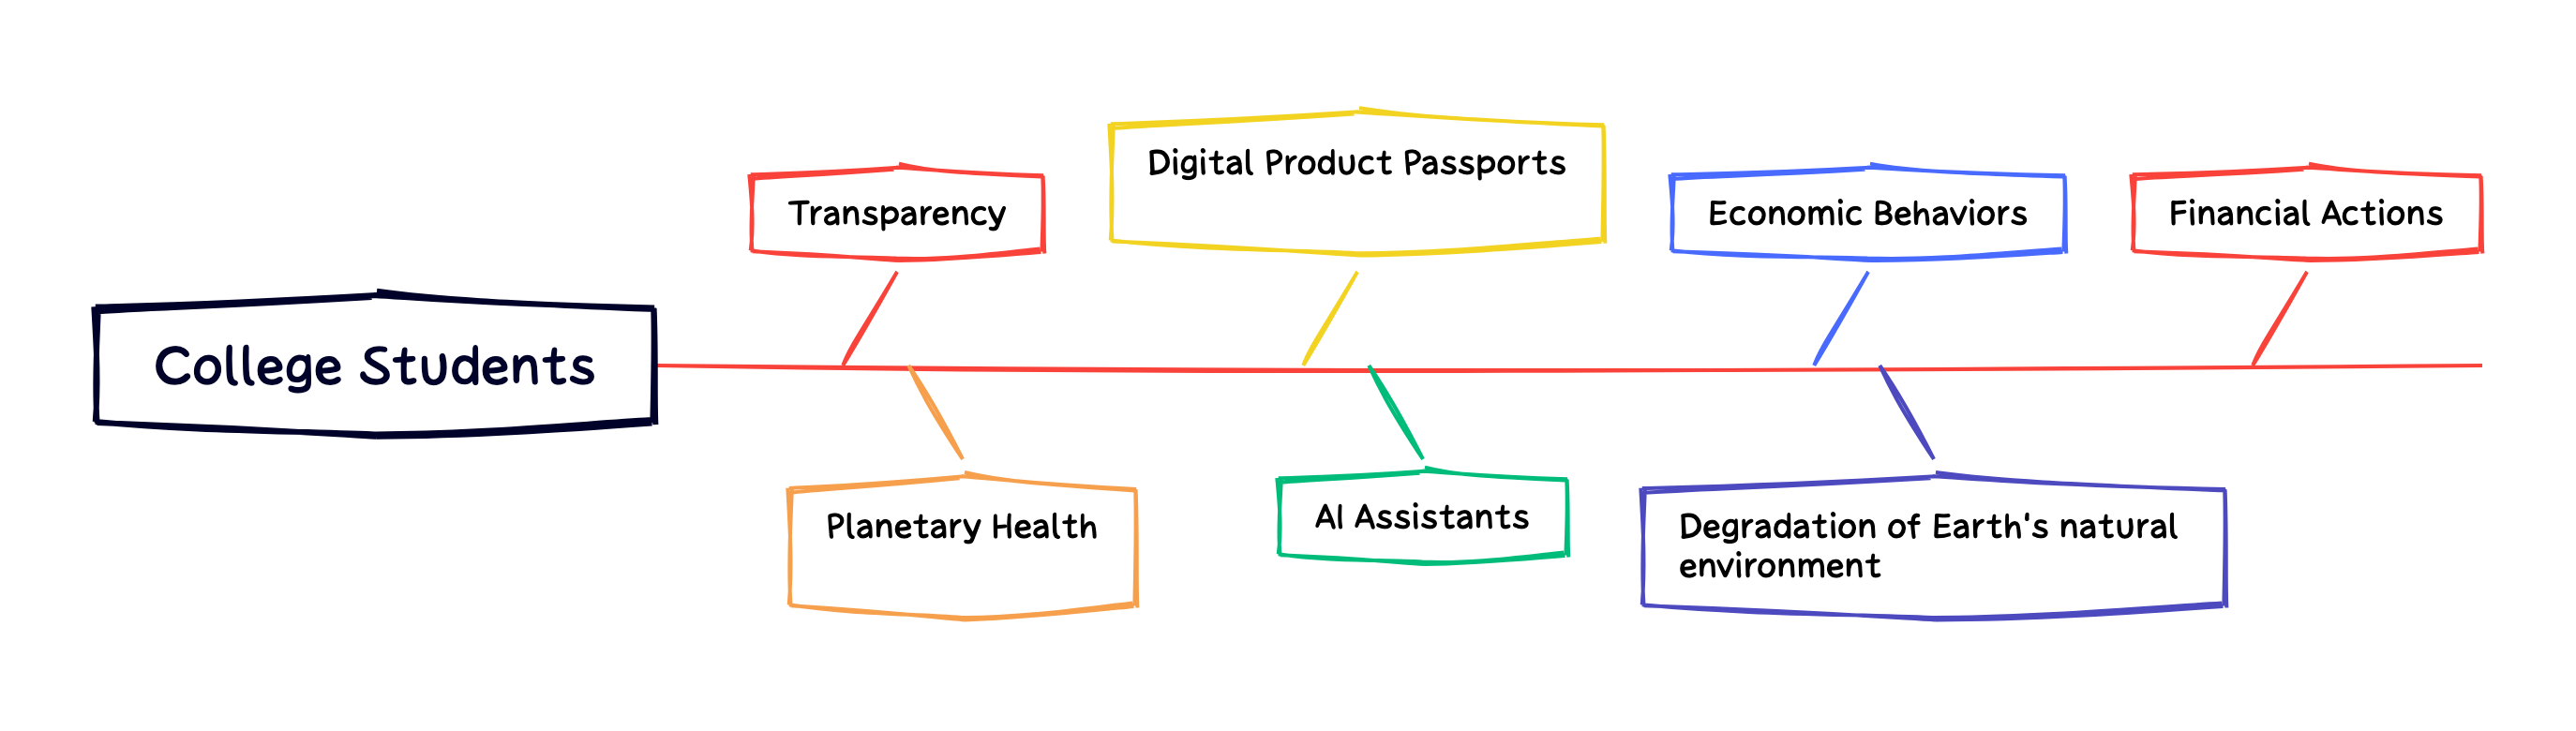
\includegraphics[width=1\textwidth,height=\textheight]{./images/introduction/abstract.png}

}

\caption{College Students}

\end{figure}%

\subsection{Relevance}\label{relevance}

The research addresses the \textbf{\emph{``attitude-behavior gap''}}
among Taiwanese college students in taking sustainable financial action.

Convergence of the following 5 trends makes my research timely in 2024.

\begin{longtable}[]{@{}
  >{\raggedright\arraybackslash}p{(\columnwidth - 2\tabcolsep) * \real{0.4167}}
  >{\raggedright\arraybackslash}p{(\columnwidth - 2\tabcolsep) * \real{0.5833}}@{}}
\caption{Trending narratives.}\tabularnewline
\toprule\noalign{}
\begin{minipage}[b]{\linewidth}\raggedright
Trend
\end{minipage} & \begin{minipage}[b]{\linewidth}\raggedright
Direction
\end{minipage} \\
\midrule\noalign{}
\endfirsthead
\toprule\noalign{}
\begin{minipage}[b]{\linewidth}\raggedright
Trend
\end{minipage} & \begin{minipage}[b]{\linewidth}\raggedright
Direction
\end{minipage} \\
\midrule\noalign{}
\endhead
\bottomrule\noalign{}
\endlastfoot
Environmental degradation & Worsening \\
Interest in sustainability among young people & ? \\
Intergenerational money transfer; in some countries relatively young
people have money & ? \\
Availability of sustainability tools such as ESG, B Corporations, Green
Bonds, etc, among metrics and instruments & Increasing \\
Availability of generative AI-based user interfaces (UIs) &
Increasing \\
Democratization of Financial Markets & Increasing \\
\end{longtable}

\subsection{Background}\label{background}

I grew up as an avid science fiction reader, which influenced my outlook
towards future possibilities. In particular, the Star Trek universe had
an imaginary portable device called a \textbf{\emph{tricorder}} (fig.~1)
enabling scientists to scan anything for insights. Be it precious
minerals inside a cave or scanning the human bodies for medical data,
its sensors would show up with some useful data. In daily life, I would
love to have such a device for consumer choices and financial decisions
- to know what to buy and which businesses to support with my money and
approval.

\begin{figure}[H]

{\centering 
\includegraphics[width=0.5\textwidth,height=\textheight]{./images/introduction/tricorder.jpg}

}

\caption{Captain Sulu using a Tricorder (Star Trek) - Photo copyright by
Paramount Pictures}

\end{figure}%

While a \emph{tricorder} is still science fiction, technological
advancements are getting closer and closer to producing something
similar. AIs are already integral to many parts of our lives, with
computer models producing increasingly useful outputs. The proposal for
this thesis was first written using Google's and Apple's voice
recognition software in 2020, and later switching to OpenAI's
\emph{Whisper} model, allowing me to transcribe notes with the help of
an AI assistant. As a foreigner living in Taiwan since 2019, I relied on
AI-based tools for many aspects of my life: speaking, moving, finding
food and services. When writing in Chinese, Apple's text prediction
algorithms translate pinyin to 漢字 and show the most likely character
based on my previous writing, Google's maps find efficient and
eco-friendly routes and recommend places to eat and ChatGPT provides
statistically probable advice from the sum of human knowledge. Even when
we don't realize it, AI is helping us with many mundane tasks. While it
takes incredibly complex computational algorithms to achieve all this in
the background, it's become so commonplace, we don't even think about
it. From this point of view, another AI assistant to help students with
choosing more eco-friendly businesses - to shop, save, and invest -
doesn't sound so much of a stretch.

\subsection{Motivation}\label{motivation}

Environmental degradation is increasingly affecting human lives - and
it's largely driven by manufacturing processes - of the products we
consume daily. From resource extraction in the linear economy (mining
raw materials and drilling for fossil fuels) to chemical processes
(causing contamination and pollution of the air, water, and soil) to
waste generation and greenhouse gas emissions, industries transform the
natural world into consumer products. While industry practices have
improved since the industrial revolution in the 19th century, and
continue to improve, it's possible to further improve standards of
production and raise the global baseline for sustainability, given
enough societal pressure to do so.

Nonetheless, without easily accessible and reliable data, it's difficult
to know which company is more sustainable than another. As consumers and
investors (even if only through passive ownership of savings), we don't
really know much about enterprise production practices, unless we spend
a lot of time looking at the numbers, which may be costly to access (for
example ESG reports are expensive), and mostly rely on our governments
and international bodies to keep us safe. Or just look at the brands
themselves - and pick the ones which we like.

\subsection{Objective}\label{objective}

The study presents design research for developing an AI companion to
help college students find sustainable companies for shopping, saving
and investing. The major contribution of my study is an interactive
artefact (a prototype) informed by design research.

\subsection{Demographics}\label{demographics}

The research focuses on young adults, specifically Taiwanese college
students studying in Taiwan.

\begin{longtable}[]{@{}ll@{}}
\toprule\noalign{}
Criteria & \\
\midrule\noalign{}
\endhead
\bottomrule\noalign{}
\endlastfoot
Location & Taiwan \\
Population & College Students \\
Count & 700 \\
\end{longtable}

Experts (finance, design, sustainability).

\begin{longtable}[]{@{}ll@{}}
\toprule\noalign{}
Criteria & \\
\midrule\noalign{}
\endhead
\bottomrule\noalign{}
\endlastfoot
Location & Global \\
Population & Experts \\
Count & 5 \\
\end{longtable}

\subsection{Research Questions}\label{research-questions}

My research answers the following questions.

\begin{longtable}[]{@{}
  >{\raggedright\arraybackslash}p{(\columnwidth - 2\tabcolsep) * \real{0.5556}}
  >{\raggedright\arraybackslash}p{(\columnwidth - 2\tabcolsep) * \real{0.4444}}@{}}
\caption{RQs.}\tabularnewline
\toprule\noalign{}
\begin{minipage}[b]{\linewidth}\raggedright
Question
\end{minipage} & \begin{minipage}[b]{\linewidth}\raggedright
Methods
\end{minipage} \\
\midrule\noalign{}
\endfirsthead
\toprule\noalign{}
\begin{minipage}[b]{\linewidth}\raggedright
Question
\end{minipage} & \begin{minipage}[b]{\linewidth}\raggedright
Methods
\end{minipage} \\
\midrule\noalign{}
\endhead
\bottomrule\noalign{}
\endlastfoot
What scientific knowledge in sustainability, design, and finance could
an AI companion integrate to support college students? & Literature
Review \\
How would college students use an AI companion to allocate capital to
sustainable companies when shopping, saving, and investing? & Literature
Review and Expert Interviews \\
How would college students prioritize specific AI companion features? &
Survey of College Students \\
\end{longtable}

\begin{itemize}
\item
  What factors increase potential users choosing sustainable investing?
\item
  What class of investment vehicles do potential users show the most
  interest in?
\item
  What application features do potential users rate as the highest
  priority?
\end{itemize}

\newpage

\subsection{Literature Review}\label{literature-review}

\subsubsection{Goals}\label{goals}

Given the goal of designing an app to integrate sustainable shopping,
saving, and investing. The goal of the literature review is to find
insights about the target audience (Taiwanese college students),
understand what kind of sustainable actions are effective, and translate
these into specific ideas for app features. In order to keep track more
easily, each literature review chapter includes in-context \emph{design
implications}.

The literature review branches out to 5 main directions and maps out
relationships sources and the literature map, namely Taiwanese college
students, generation-z demographics, sustainability, ecology, ecosystem
services, EU legislation, sustainable finance, sustainable investing,
savings, circular economy, economics, AI, existing sustainability,
software, sustainability--related mobile apps (Apple iOS / Google
Android), and web apps related to sustainable shopping, savings, and
investing; apps using algorithmic interfaces (AI-based UI), design,
UX/UI, service design, sustainable design, speculative design,
interaction design, behavior change, nudge.

\begin{figure}[H]

{\centering 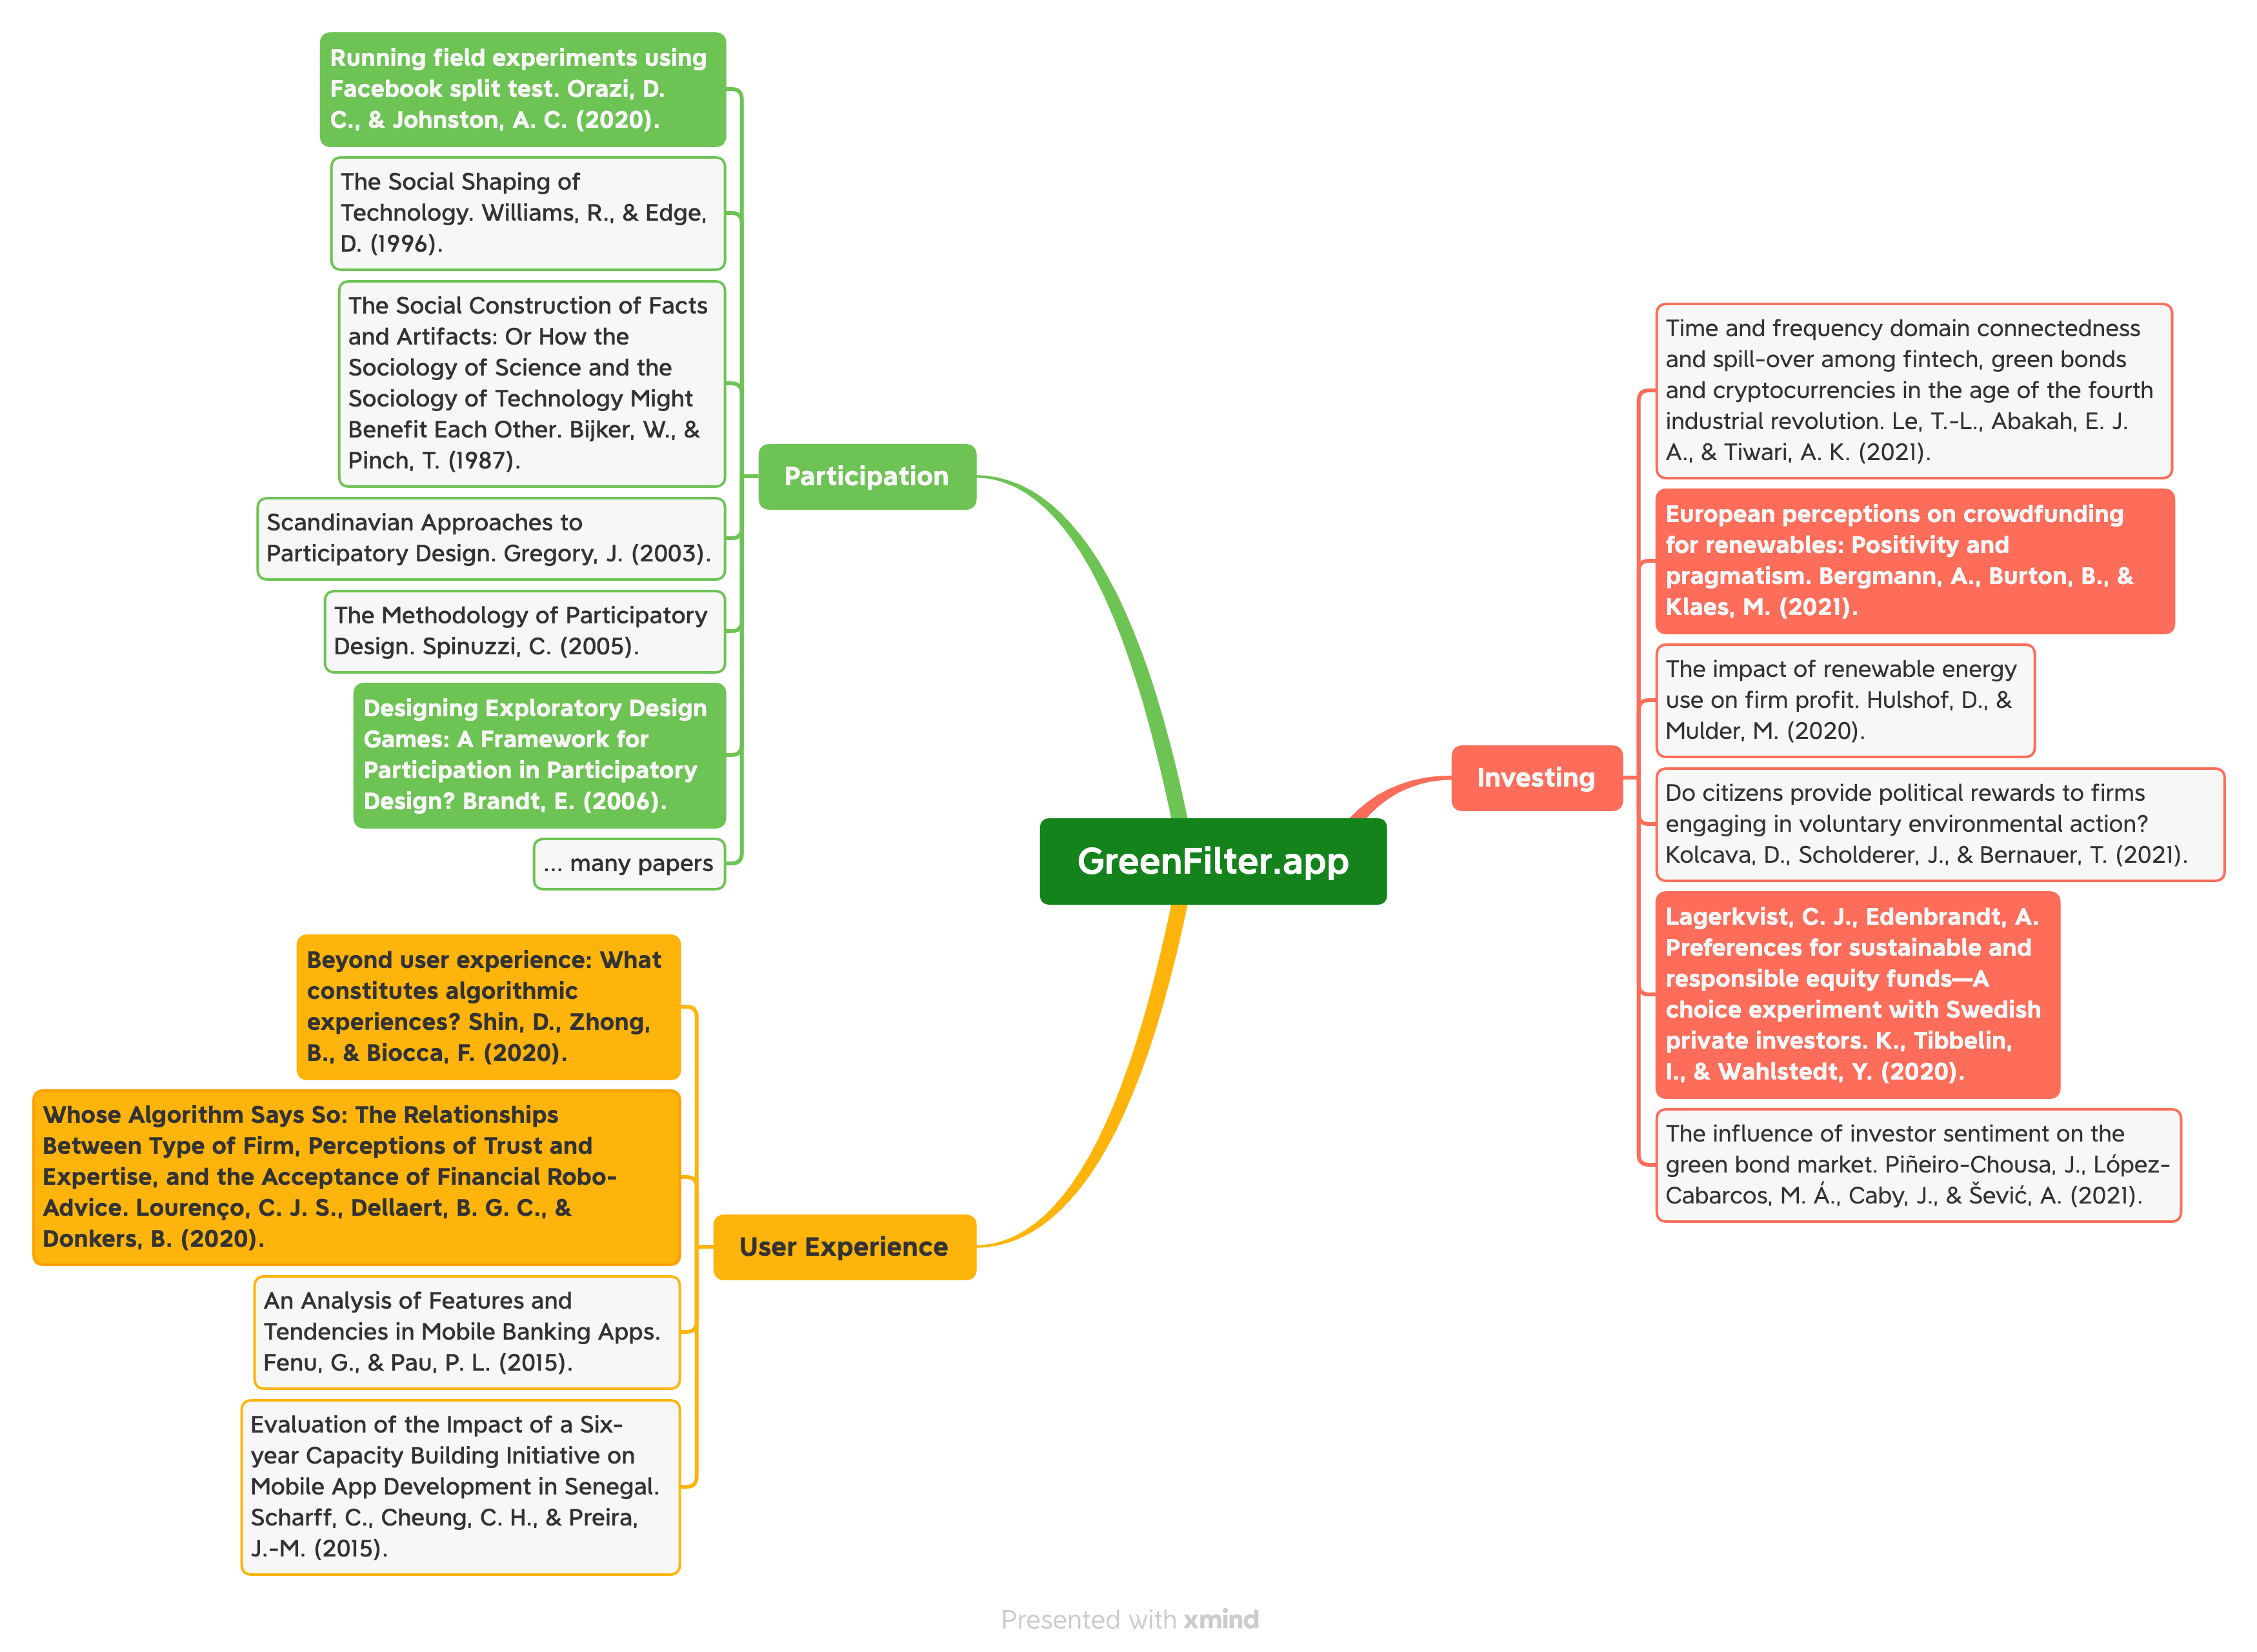
\includegraphics[width=1\textwidth,height=\textheight]{./images/literature/literature.png}

}

\caption{Example papers from the Literature Review}

\end{figure}%

\subsubsection{Sources}\label{sources}

There is currently no single platform that hosts all scientific journals
leading me to source scientific papers from

\begin{itemize}
\tightlist
\item
  ScienceDirect
\item
  Nature
\item
  the Lancet
\item
  Oxford Academic
\item
  Semantic Scholar
\item
  JSTor
\item
  Google search.
\end{itemize}

\subsubsection{AI Usage in Research}\label{ai-usage-in-research}

I'm a long time AI-assistant user. AI was used for

\begin{itemize}
\tightlist
\item
  search
\item
  data comparison
\item
  data science
\item
  chart-building
\end{itemize}

AI was \emph{NOT} used for writing.

\newpage

\section{Students}\label{students}

\subsection{Research Gap When it Comes to Taiwanese College
Students}\label{research-gap-when-it-comes-to-taiwanese-college-students}

There's lack of scientific research when it comes to Taiwanese college
students, not only in English or other foreign languages, but also in
Chinese. Much of the research in Taiwan focuses on younger students,
particularly those in primary and secondary schools. With regards to
issues related to college students and sustainability, even less
research is available. My project hopes to shed some light to how
Taiwanese college students relate to sustainability.

\subsection{Taiwan in the Global Context: Global and Local
Attitudes}\label{taiwan-in-the-global-context-global-and-local-attitudes}

(Kuo-Hua Chen, 2019) compares Taiwan to other countries in terms of
Postmaterialist Index Comparison, noting Taiwanese society is
materalistic.

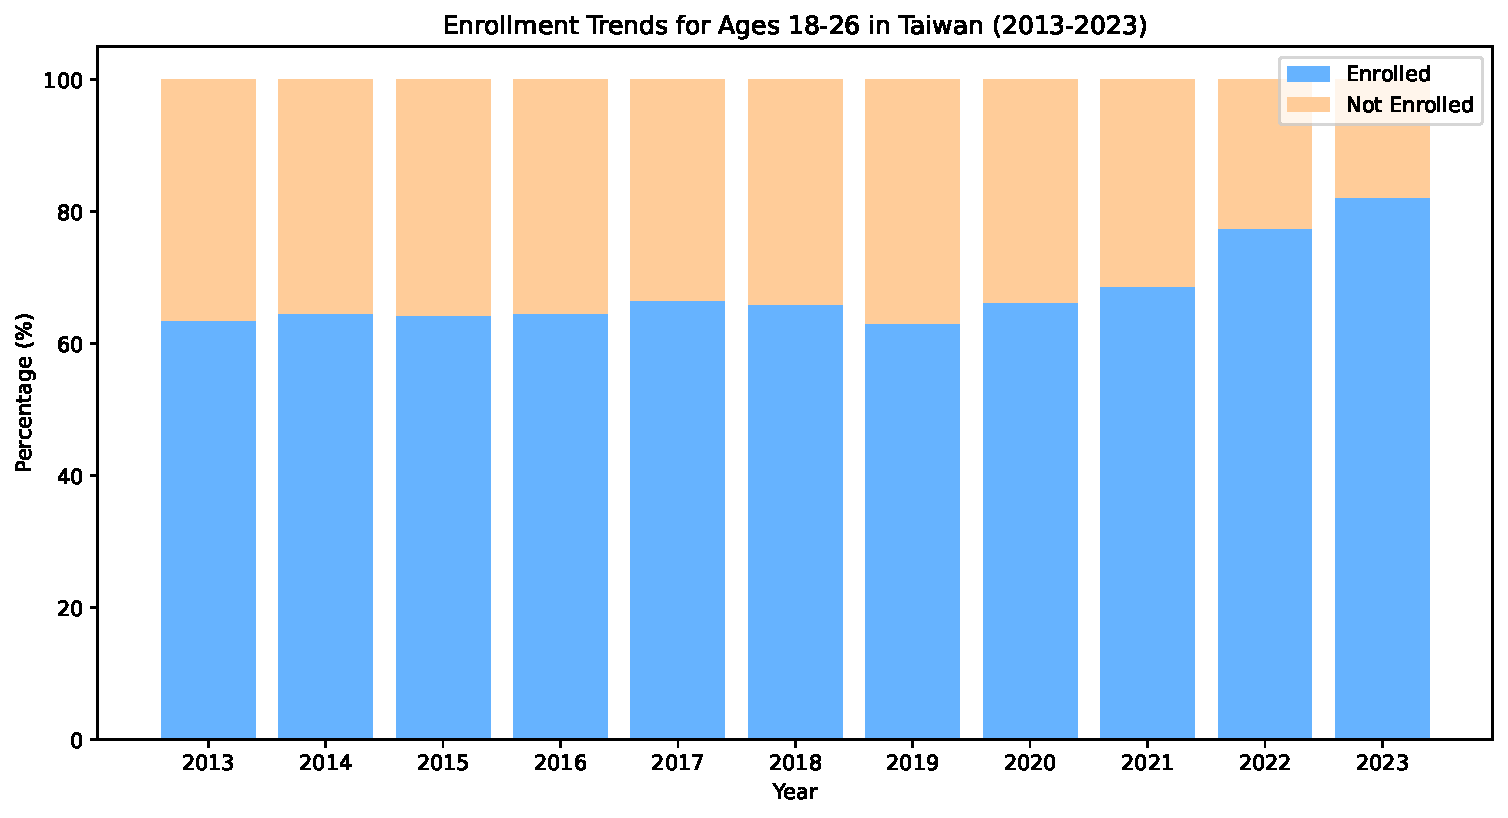
\includegraphics{_thesis_files/figure-pdf/cell-4-output-1.pdf}

World Values Survey

\includegraphics{_thesis_files/figure-pdf/cell-5-output-1.pdf}

(Franzen \& Bahr, 2024) measures \emph{``mean environmental concern''}
to look at decade-level changes in societal environmental attitudes
across countries. Taiwan's general attitudes have stayed almost the same
(slight increase). The UK has had the largest jump in concern.
Curiously, South Korea has had a slight decrease in concern. Slovakia
and Russia were not very concerned with the environment a decade ago and
are even less concerned now.

A large-scale global study by (Anthony Leiserowitz et al., 2022)
administered on Meta's Facebook (n=108946) reported people in Spain
(65\%), Sweden (61\%), and Taiwan (60\%) believe \emph{``climate change
is mostly caused by human activities''.}

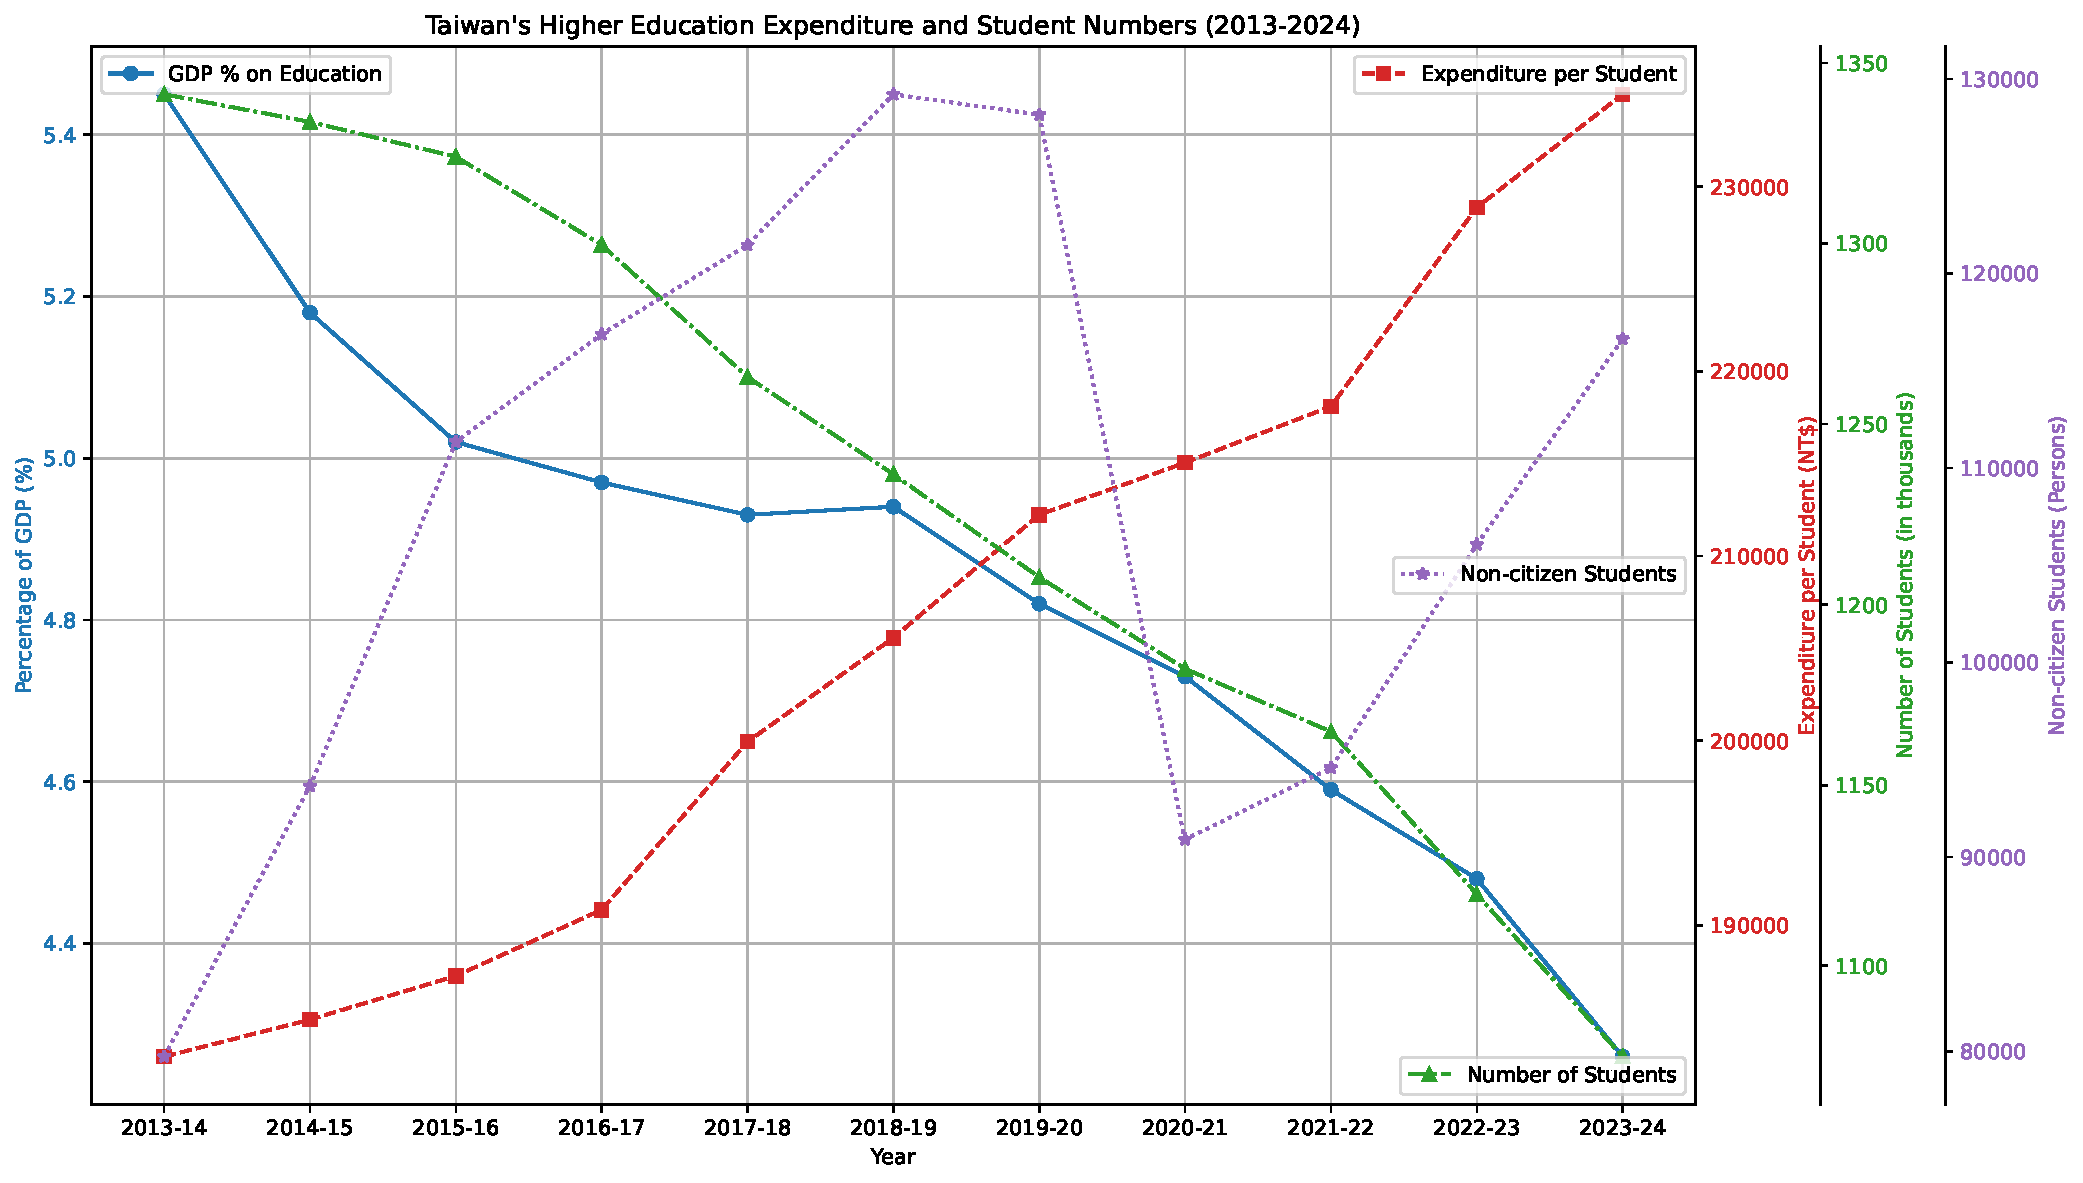
\includegraphics{_thesis_files/figure-pdf/cell-6-output-1.pdf}

The largest study to date, conducted by the United Nations across 50
countries, surveying 1.2 million people, distributed through mobile game
ads, showed the majority of people agreeing climate change is an
\emph{``emergency''} (UNDP, 2021).

\begin{longtable}[]{@{}lll@{}}
\caption{1.2 million UN survey responses to the statement
\emph{``Climate change is an emergency''} (UNDP, 2021).}\tabularnewline
\toprule\noalign{}
\endfirsthead
\endhead
\bottomrule\noalign{}
\endlastfoot
Age Group & Agree & Neutral or Disagree \\
18-35 & 65\% & 35\% \\
36-59 & 66\% & 34\% \\
Over 69 & 58\% & 42\% \\
\end{longtable}

\subsection{Student Protests: In Taiwan vs Around the
World}\label{student-protests-in-taiwan-vs-around-the-world}

In August 2018, Swedish high-school student Greta Thunberg skipped class
to start a climate strike in front of the Swedish parliament Riksdag.
Millions of people around the world joined her \emph{Fridays for Future}
protests. Time magazine named Thunberg person of the year for
\emph{creating a global attitudinal shift.} (Deutsche Welle, 2019).

\begin{figure}[H]

{\centering 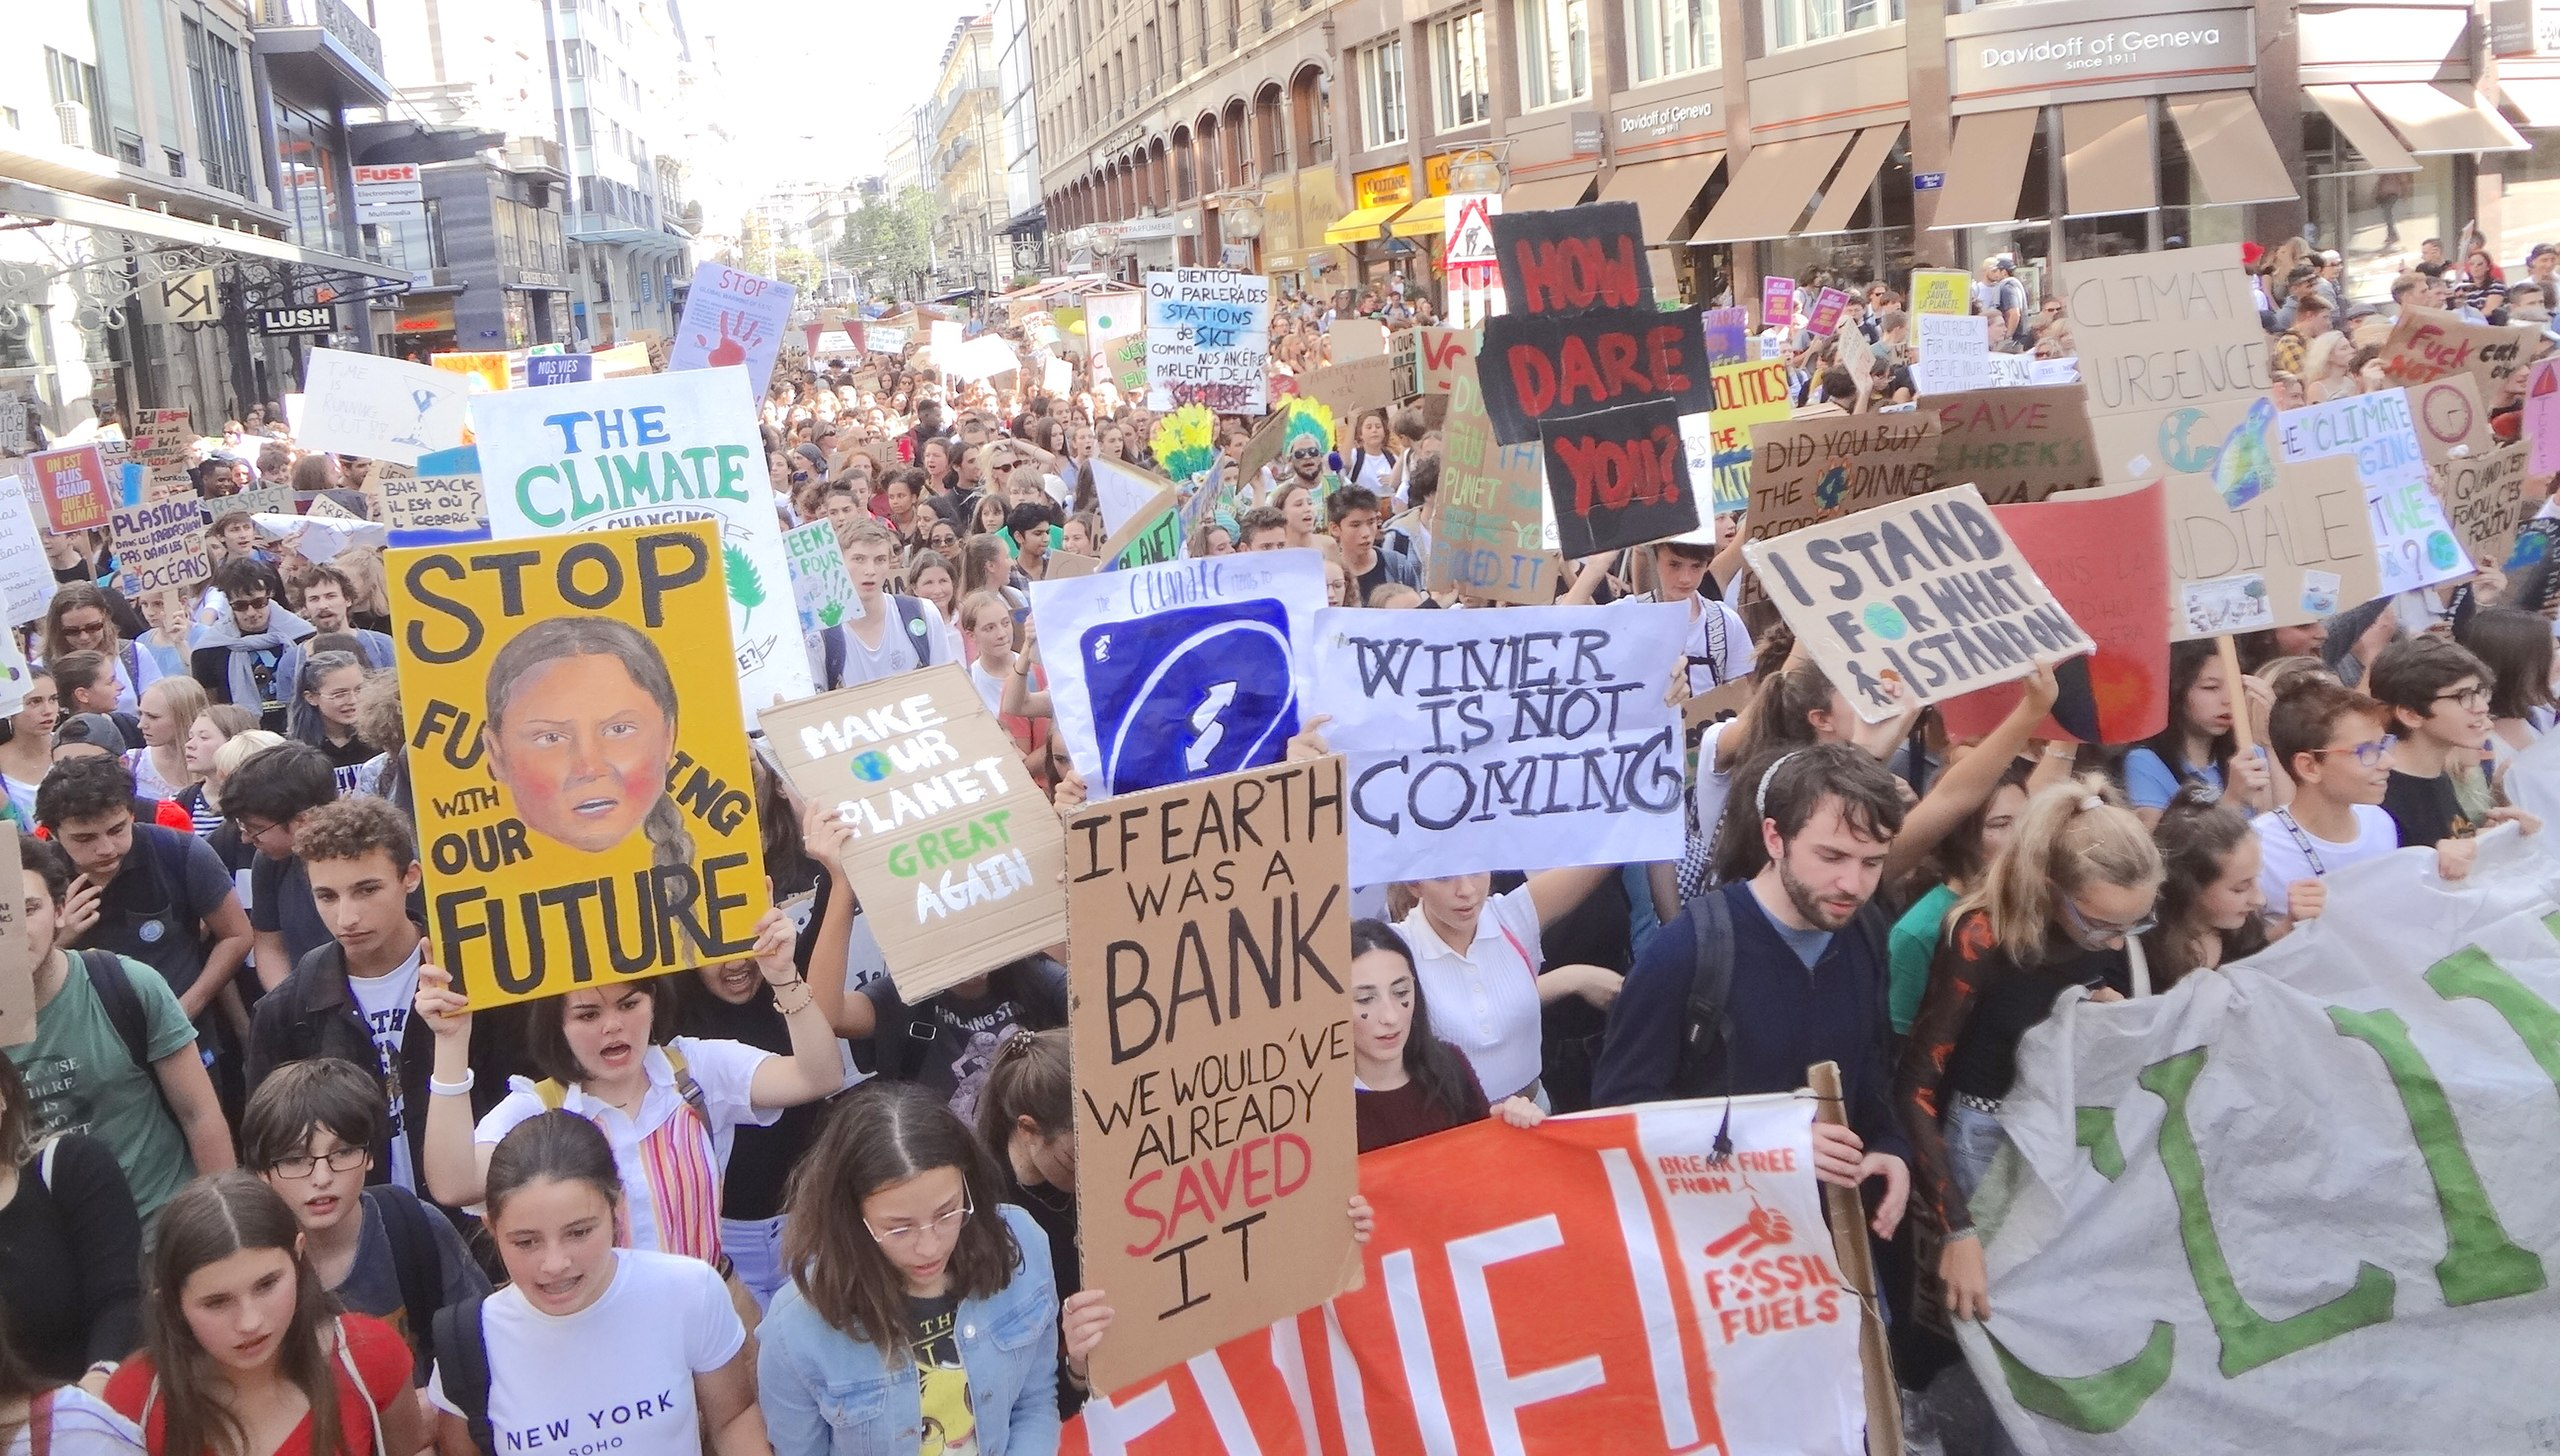
\includegraphics[width=1\textwidth,height=\textheight]{./images/college/geneve.jpg}

}

\caption{Climate protest in Geneva on 27th September, 2019 -- 1 year
after the start of Fridays for Future}

\end{figure}%

In Taiwan, the Fridays for Future protests were small in scale, with no
more than 100-200 people (Hioe, 2019). Meanwhile 2000 Taiwanese students
joined the initative by participating in environmental activities
without protesting
{[}daiQuanQiuXueShengQiHouYunDongTaiWanXueShengZouChuZiJiDeLu2019{]};

\begin{figure}[H]

{\centering 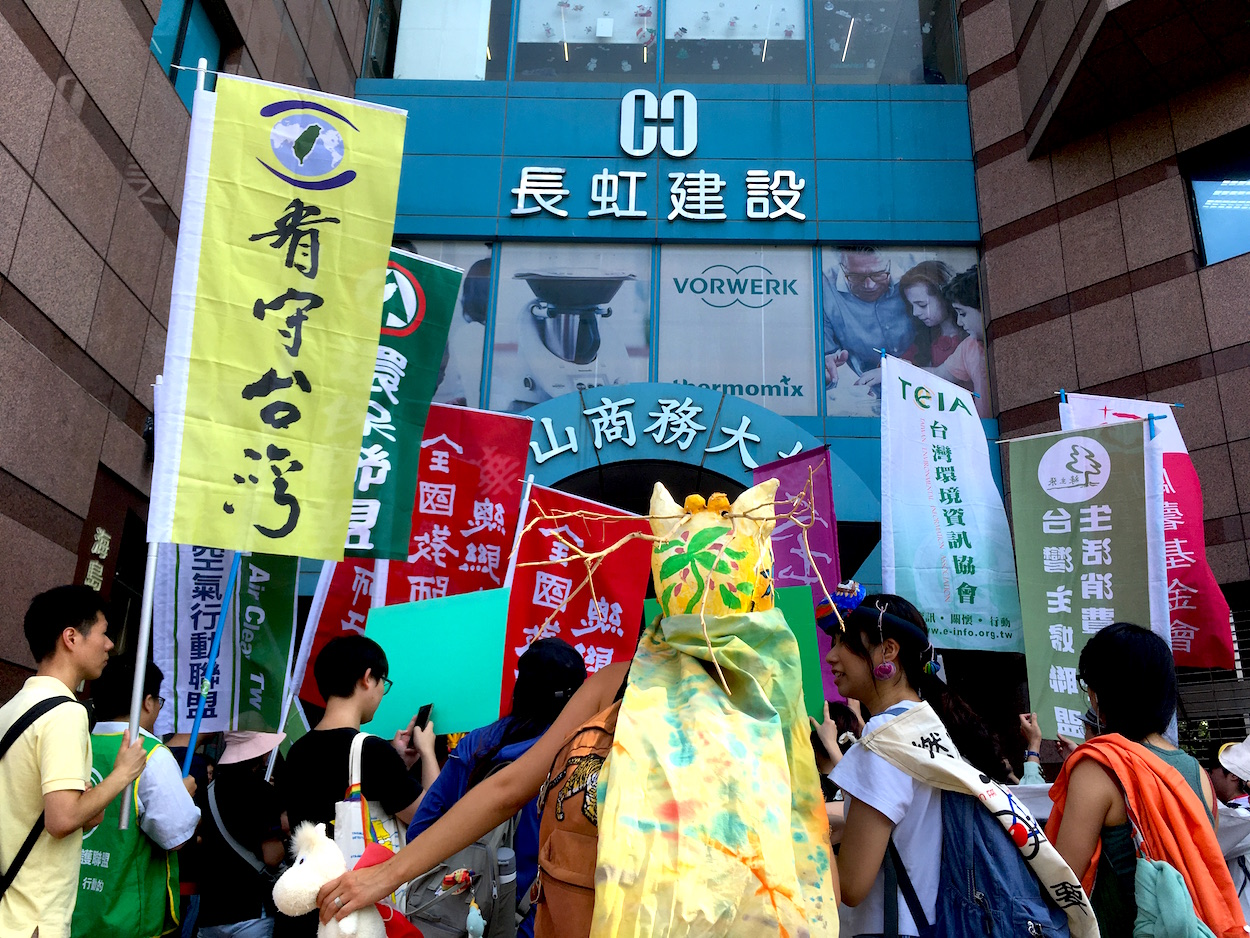
\includegraphics[width=1\textwidth,height=\textheight]{./images/college/taipei.jpg}

}

\caption{Climate protest in Taipei in May 2019 in front of the
Democratic Progressive Party (DPP) headquarters}

\end{figure}%

Meanwhile Indonesia, Philippines, have had larger protests.

The protest trend is subsiding.

McKinsey says people want eco-products but aren't willing to pay more.

Willingness too pay research.

\subsection{The Attitude-Behavior Gap}\label{the-attitude-behavior-gap}

While people express eco-conscious ideas, it's non-trivial to practice
sustainability in daily life. (Deyan Georgiev, 2023b) reports only 30\%
of people in the Gen-Z age group believe technology can solve all
problems.

\begin{itemize}
\tightlist
\item
  (Park \& Lin, 2020) positive attitude towards sustainable products
  does not result in purchase decisions, shows research of fashion in
  South Korea. In one Australian study, green consumers still waste food
  similarly to the baseline (McCarthy \& Liu, 2017).
\item
  Munro, Kapitan \& Wooliscroft (2023) shoppers trying to shop
  sustainably often fail to find sustainable products.
\item
  Marc Lien (2022) Four millions British SMEs have no plan for net-zero
  transition.
\item
  Ware (2024) British workers lack skills for green transition. (2024
  National Environmental Services Survey)
\end{itemize}

\subsection{Credit Cards}\label{credit-cards}

\begin{itemize}
\tightlist
\item
  an older study, I-Cheng Yeh (2009) provides data from credit card
  usage from an unnamed ``important'' bank in Taiwan. Because of the age
  of the study there's no Gen-Z data. People aged 18-26 at the time
  would be Millenials or Gen-X by now.
\end{itemize}

data donated (Yeh, 2016).

https://www.semanticscholar.org/paper/The-comparisons-of-data-mining-techniques-for-the-Yeh-Lien/1cacac4f0ea9fdff3cd88c151c94115a9fddcf33

\subsection{Taiwanese Education System and Policy
Environment}\label{taiwanese-education-system-and-policy-environment}

Taiwan has approximately 2 million young adults (Gen-Z, 18-26), and 73\%
percent of them are students attending tertiary education as of 2023,
with a slow increase of enrollment over the past decade (Ministry of
Education of Taiwan, 2024b).

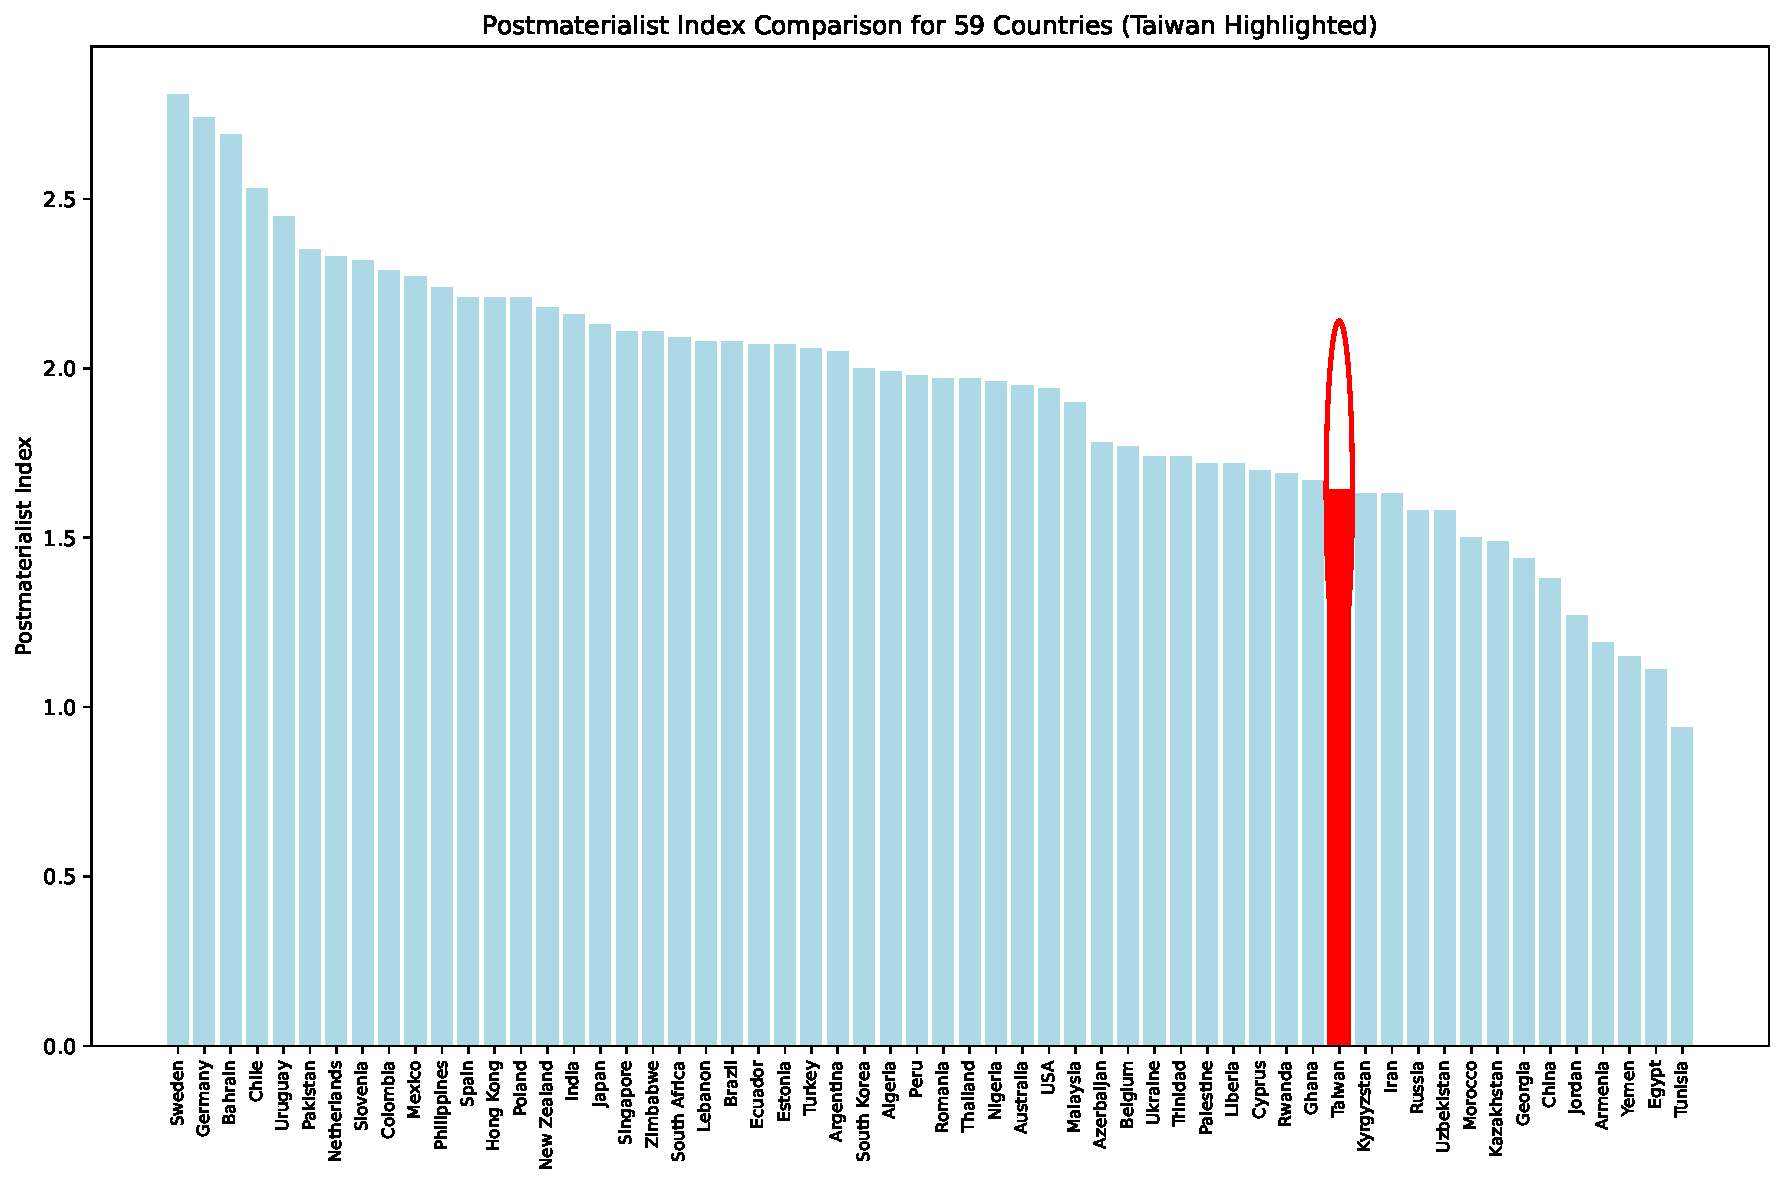
\includegraphics{_thesis_files/figure-pdf/cell-7-output-1.pdf}

As of 2024, Taiwan has a total of 148 universities, colleges, and junior
colleges (Ministry of Education of Taiwan, 2024c). Education funding is
4.26\% of Taiwan's GDP in 2023-24 and has been on a decline for a decade
(Ministry of Education of Taiwan, 2024a). Taiwan has an aging population
and declining birth rates have forced several schools to close down (Goh
et al., 2023; Davidson \& Chi-hui, 2024).

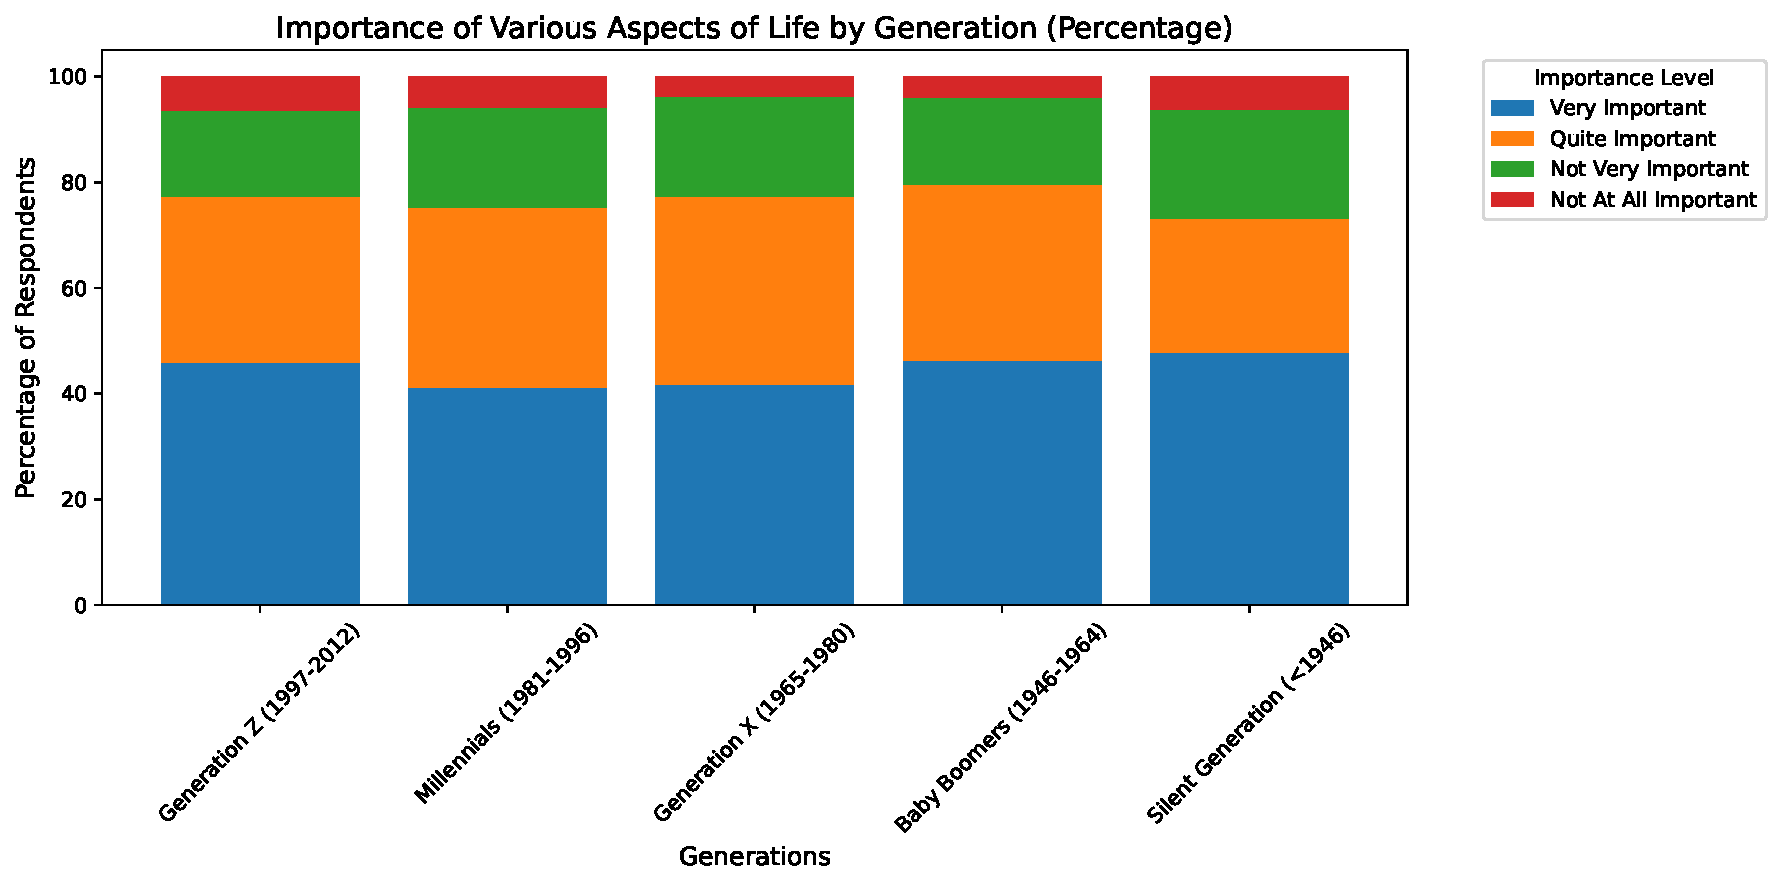
\includegraphics{_thesis_files/figure-pdf/cell-8-output-1.pdf}

While the overall number of students is declining, the share of
international students is increasing.

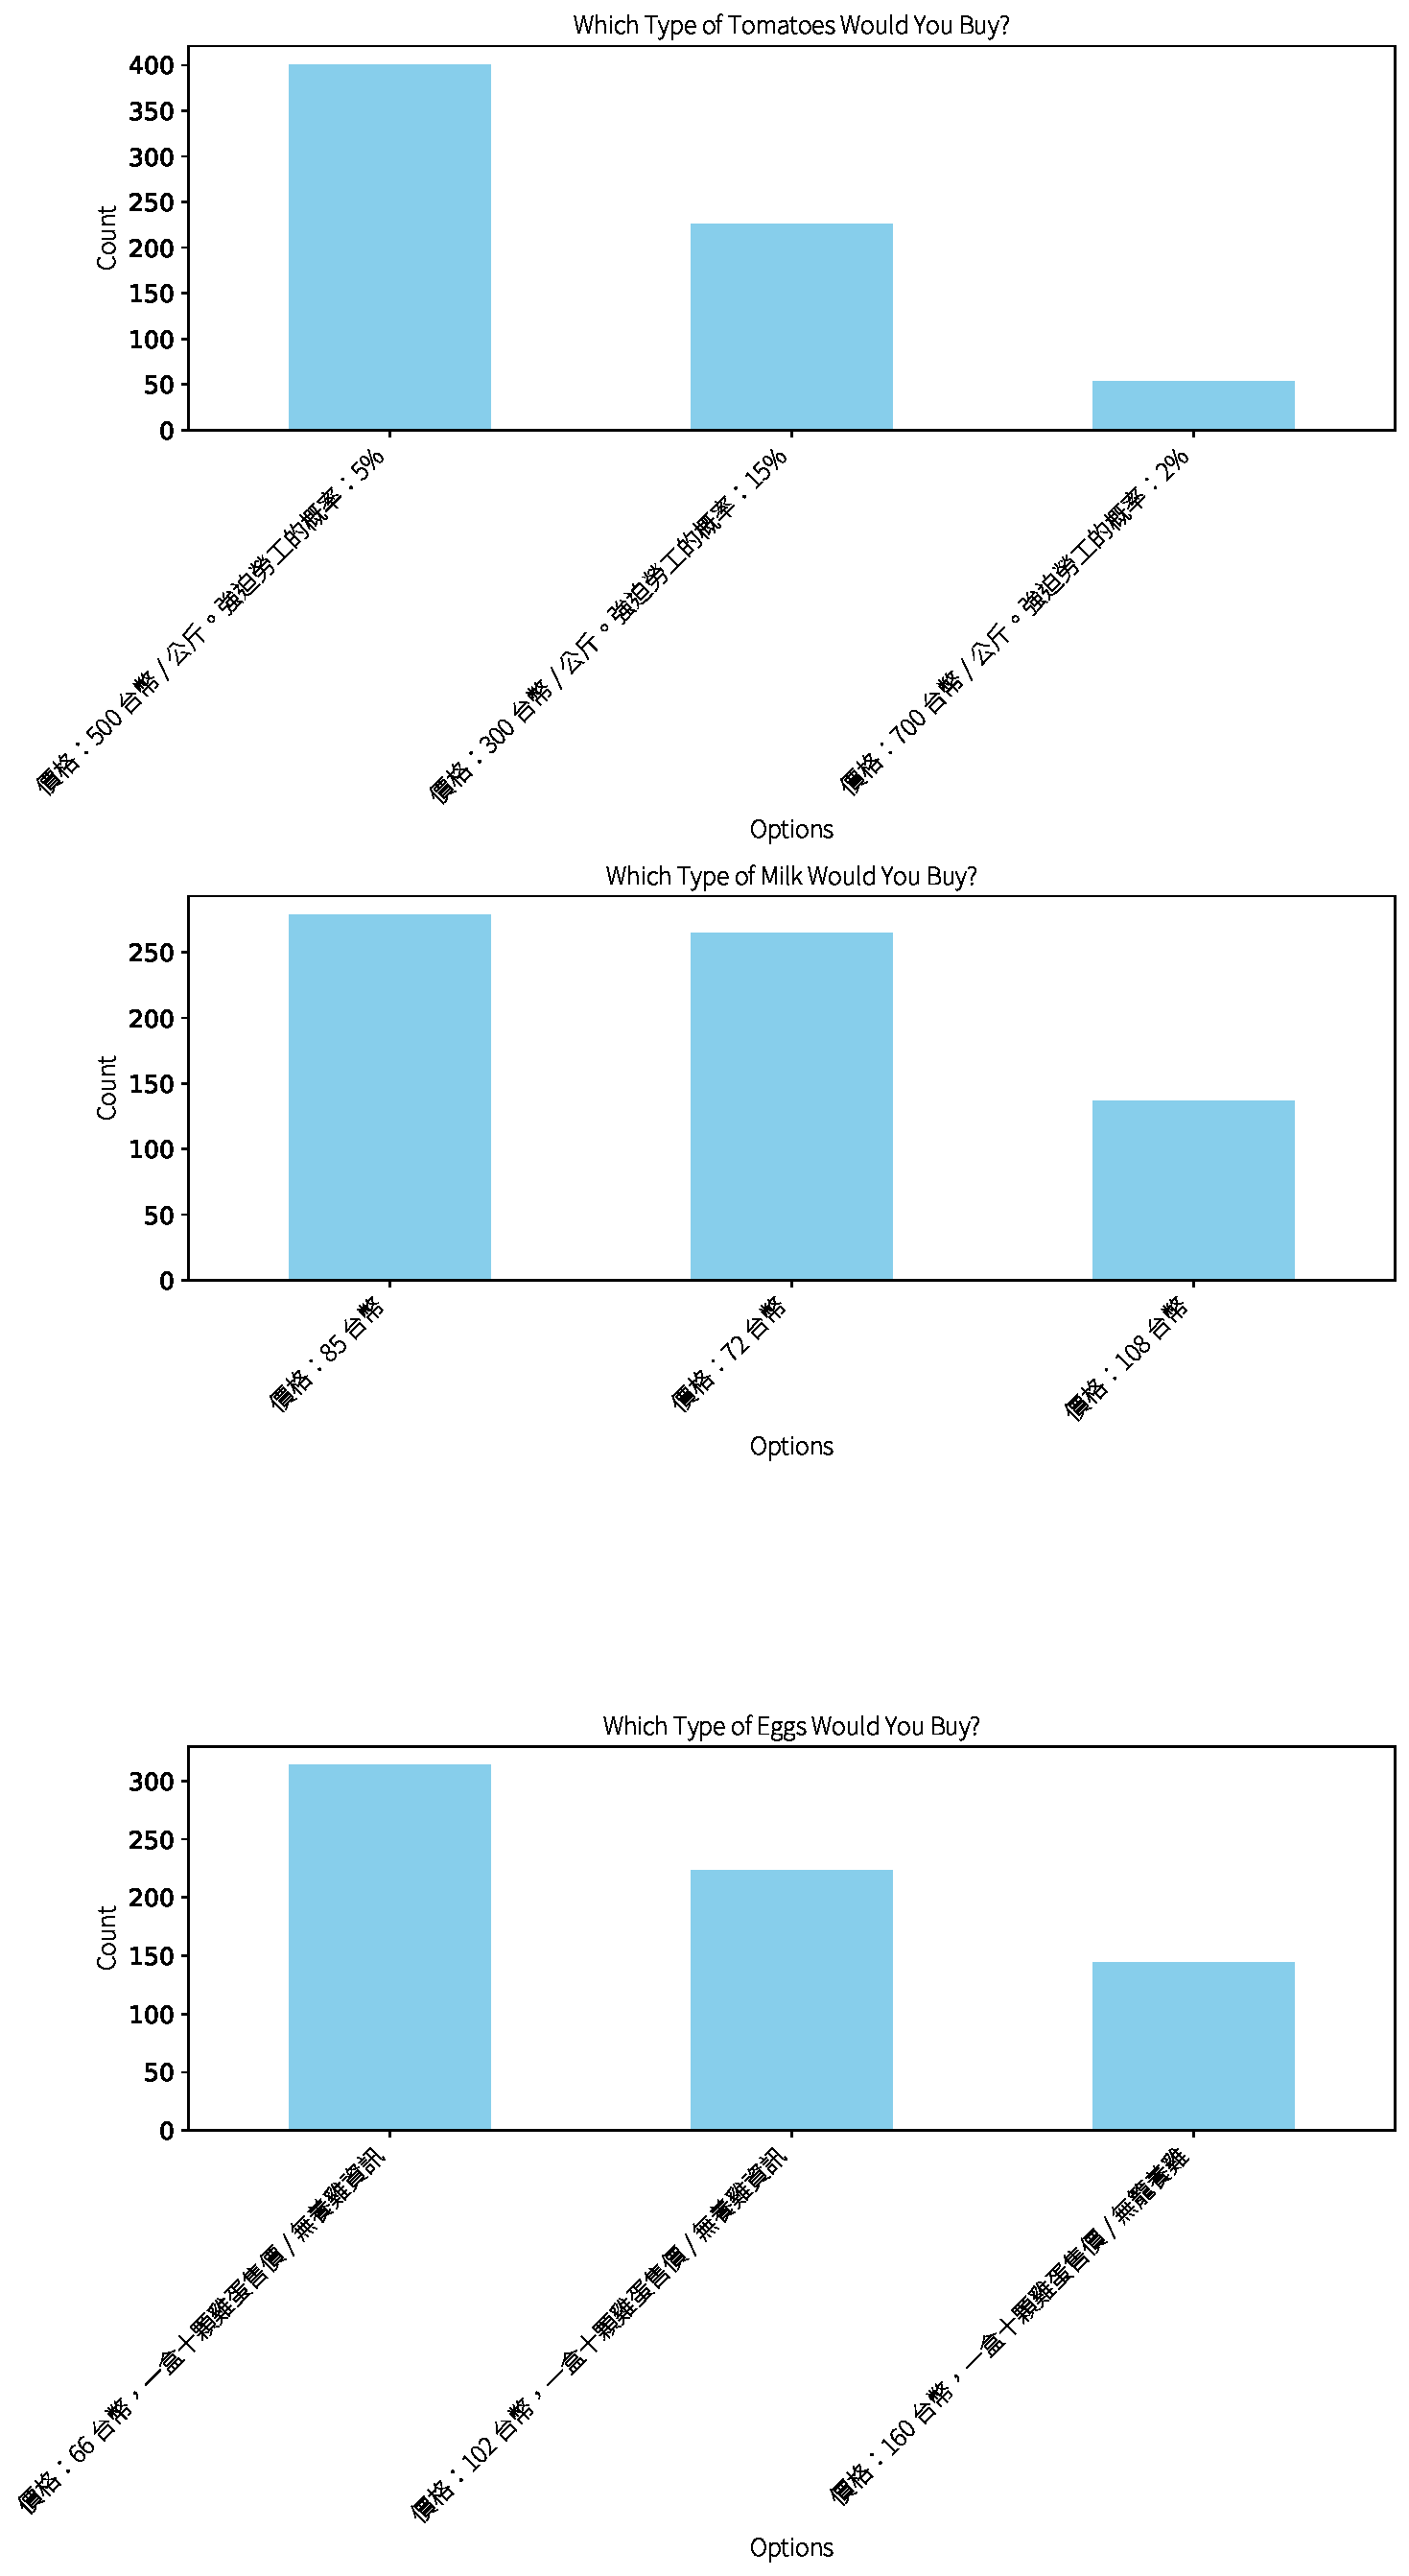
\includegraphics{_thesis_files/figure-pdf/cell-9-output-1.pdf}

\subsubsection{Confucianism}\label{confucianism}

Taiwanese culture is deeply influenced by Confucianism, valuing academic
excellence, effort, and the role of education in achieving social status
(Xu, 2024). Both Confucianism and Daoism affect education to be
\emph{teacher-centered}, where traditionally the role of students is to
listen and absorb knowledge; in today's society, there's space to open
opportunities for revisiting \emph{dialogue-based} education, where
students would be encouraged to take a more active role and gain
ownership of their education (Chang, Wegerif \& Hennessy, 2023).

\subsubsection{Sustainability Attitudes}\label{sustainability-attitudes}

In general, Taiwanese teachers at all levels of education have a
positive attitude towards sustainability.

At the pre-university level, Taiwanese government has been promoting
environmental education through a green school network; however surveys
at middle school and high school level suggest there is no impact on
\emph{sustainability consciousness} among students in comparison with
regular schools (Olsson et al., 2019). Rather, Taiwanese students are
influenced towards environmental action by \emph{group consciousness}
(Yu, Yu \& Chao, 2017). In contrast,(陳珮英, 2003) reports \emph{good
knowledge of sustainable development} topics among \emph{junior high
school students} in Da-an District, Taipei City (n=596). (林, 2009)
similarly reports a positive attitude and good knowledge of
environmental sustainable development among senior \emph{high school
students} towards in Taipei City (n=328). Several Taiwanese studies also
focus on the physical environment of school campuses, for example the
sustainability of elementary school campuses (潘智謙 \& Pan, 2006).
Elementary-school teachers in Taichung (n=536), have positive attitudes
towards environmental education are positive, proactive and demonstrate
high awareness; they have participated in many sustainability-related
workshops (Liao et al., 2022).

At the university level, (Chen \& Tsai, 2016) reports a \emph{positive
attitude yet moderate knowledge} about \emph{ocean sustainability} among
Taiwanese college students (n=825). (Liu et al., 2023a) studied
sustainability behavior of Taiwanese University students, reporting the
COVID-19 pandemic, in addition to prevalence of health issues, also
spurred more attention on environmental topics. In a similar vein, the
devastating nuclear disaster in Fukushima, Japan, after 2011 earthquake,
had an effect on Taiwanese energy and sustainability education (姚 \&
侯, 2011). Taiwanese government launched the Sustainable Council in 1997
to promote of environmental and sustainable development; a survey of
university-level teachers (n=100) in central Taiwan (Taichung, Changhua,
and Yunlin) shows a positive attitude toward environmental
sustainability among teachers however implementation of environmental
sustainability practices is from low to medium range (林 \& 莊, 2015).
Taiwanese government has also launched funding for University Social
Responsibility (USR) programs to train college students in social
innovation and local revitalization (Chen \& Chou, 2023; Liu et al.,
2022).

Comparing college students' education for sustainable development (ESD)
in Taiwan (n=617) and Sweden (n=583) found Sweden has a long history in
environmental education while in Taiwan environment became a focus area
with the 1998 educational reform (Berglund et al., 2020).

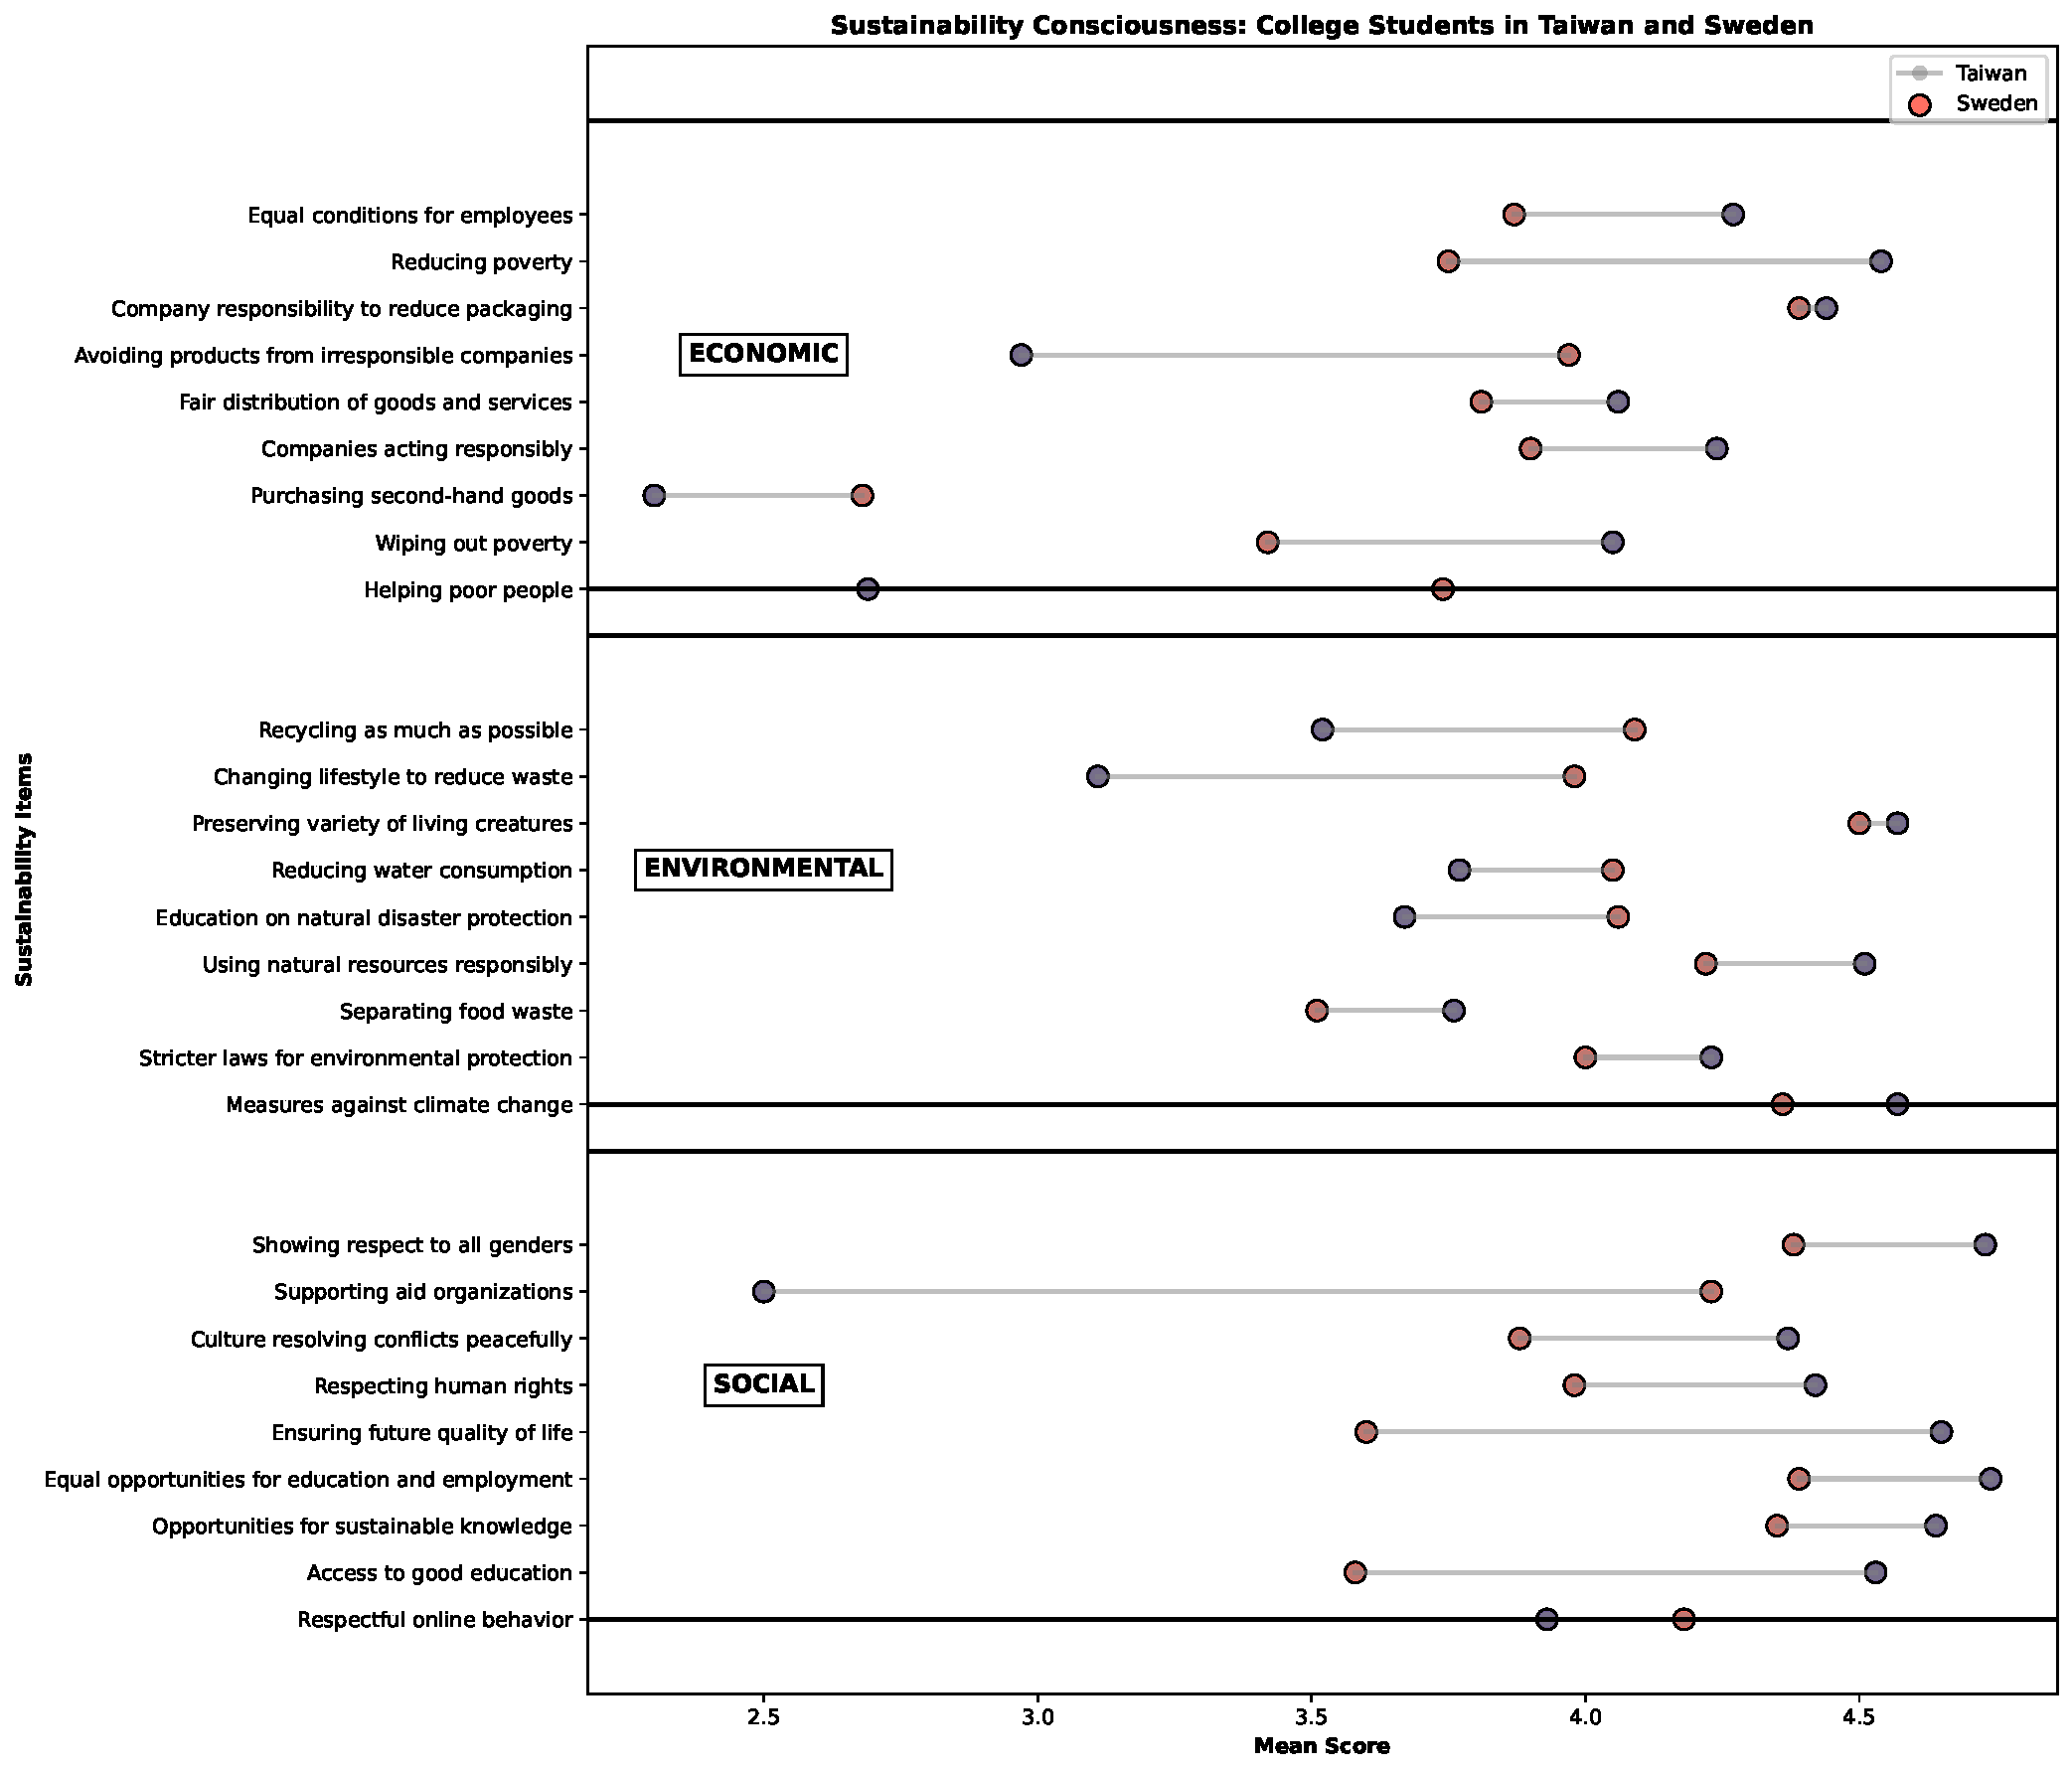
\includegraphics{_thesis_files/figure-pdf/cell-10-output-1.pdf}

\subsubsection{Eco-Friendly Diet}\label{eco-friendly-diet}

An older study in 5 university in Taipei and Taichung (n=255) found
78.04\% of respondents consumed beef in the month prior and were
concerned with food safety, freshness, and quality (Hsu, Lu \& Chen,
2014). (Thiagarajah \& Kay, 2017) reports a general observation in their
abstract (I was unable to access the full study) that most college
students in all observed countries including Taiwan (n=534) regarded
``\emph{plant-based diets to have health benefits''}.

\subsection{The Effect of Climate Change on
Taiwan}\label{the-effect-of-climate-change-on-taiwan}

Taiwan has been affected by drought over 4 decades, rising temperatures
and altered rainfall patterns, impacting water security and
semiconductor manufacturing\hspace{0pt}(Vo \& Liou, 2024). Corals
surrounding Taiwan are affected by marine heatwaves, ocean acidification
and increased sea surface temperature affects coral bleaching level (Hsu
et al., 2024). Biomarkers in the sediment core around Taiwan are being
used to study variations in climate over past thousands of years (Wang
et al., 2021). Taiwan is affected by Kuroshio (黑潮) like Estonia is
affected by the Gulf Stream. Both oceanic currents help regulate the
climates of their respective regions and marine ecosystems. Kuroshio is
a warm current of the Pacific Ocean. Rossby planetary waves driven by
the Earth's rotation are crucial to keeping the atmosphere in balance by
helping transfer tropical heat towards Earth's poles and cold air toward
the tropics; interactions between oceanic currents, Rossby waves and
nonlinear \emph{mesoscale eddies,} which form complex undulations, and
their effect on the climate are still not well understood (US Department
of Commerce, n.d.; Belonenko, Sandalyuk \& Gnevyshev, 2023; Liu et al.,
2024; Lin et al., 2022b; Yin, Lin \& Hou, 2019; Mensah et al., 2014;
Shen et al., 2014). Around 33\% of Taiwanese CO2e emissions is captured
by the marine carbon sink, while the effect of forests in Taiwan needs
further study (Hung et al., 2024).

\subsection{Sustainability Tools in the Taiwanese
Context}\label{sustainability-tools-in-the-taiwanese-context}

Musical garbage truck are a success story of the environmental progress
in Taiwan (Helen Davidson \& Chi Hui Lin, 2022). Indeed, they are a
\emph{user interface innovation} and the main way how people in Taiwan
interact with sustainability issues.

The popular narrative about Taiwan recounts the story of the economic
and environmental transformation of the country. In the late 1980s
during the heights of an economic boom Taiwan became famous as the
Taiwanese Miracle (臺灣奇蹟) (Gold, 1986; Tsai, 1999). By the early
1990s another less flattering nickname appeared: ``garbage island'', for
the piles of trash covering the streets and overflowing landfills (Rapid
Transitions Alliance, 2019; Ngo, 2020). In the two decades that
followed, from 1998 to 2018, Taiwan made progress in municipal waste
management, rising to the status of a world-leader in recycling (2nd
\emph{effective recycling rate} after Germany); in addition to an
effective recycling system, the average waste amount generated per
person by 700g (from 1140g to 400g) per day; nonetheless, industrial
recycling rates were less stellar, standing at 80\% in 2020 and there
were unrealized opportunities in using industry 4.0 technologies, such
as internet of things (IoT) sensors for better waste tracking (Wu, Hu \&
Ni, 2021; Bui et al., 2023).

Progress in sustainability is possible but achieving results takes time
and innovation. (Rapid Transitions Alliance, 2019) credits the Taiwanese
Homemakers United Foundation (財團法人主婦聯盟環境保護基金會) for
initiating the transformation in 1987, suggesting a small group of
people can have an outsized impact on the whole country. Their activity
didn't stop there and (財團法人主婦聯盟環境保護基金會, 2020) recounts a
timeline of their achievements on their website until the present day.

\subsection{Trends in Taiwanese
Companies}\label{trends-in-taiwanese-companies}

Between 1970 and 2019 CO2 was a prerequisite of economic growth in
Taiwan (check this again) (Chang et al., 2023). Taiwan is a net CO2
exporter since 1990s through emissions embedded in the industrial
production oriented economy (Huang, Lv \& Li, 2020).

TIME Magazine and Statista collaborative \emph{``World's Most
Sustainable Companies Of 2024''} includes 17 Taiwanese companies (Alana
Semuels, 2024).

\begin{longtable}[]{@{}rlr@{}}
\caption{Data from (Alana Semuels, 2024).}\tabularnewline
\toprule\noalign{}
\textbf{Rank} & \textbf{Company} & \textbf{Score} \\
\midrule\noalign{}
\endfirsthead
\toprule\noalign{}
\textbf{Rank} & \textbf{Company} & \textbf{Score} \\
\midrule\noalign{}
\endhead
\bottomrule\noalign{}
\endlastfoot
24 & Delta Electronics & 77.18 \\
63 & Taishin Holdings & 73.50 \\
68 & Fubon Financial & 73.01 \\
80 & Chunghwa Telecom & 71.69 \\
91 & Yuanta Financial Holdings & 70.94 \\
92 & Cathay Financial Holdings & 70.79 \\
108 & Taiwan Mobile & 69.72 \\
200 & First Financial Holding & 64.17 \\
300 & Far EasTone & 60.04 \\
301 & SinoPac Holdings & 60.04 \\
344 & Wistron & 58.44 \\
356 & Acer & 58.02 \\
395 & Nanya Technology & 56.35 \\
409 & InnoLux & 55.82 \\
416 & Wiwynn & 55.67 \\
421 & Taiwan Cement & 55.49 \\
497 & Advantech & 53.14 \\
\end{longtable}

Meanwhile, Corporate Knights which has been ranking global sustainable
companies since 2005, including analysis of 7000 public companies with a
revenue over US\$1 billion, only includes TSMC in the top 100 (placed
20th in 2021 and 44th in 2022, dropping out in 2023) and Taiwan High
Speed Rail Corp and Giant Manufacturing Co Ltd since 2023. (Corporate
Knights, 2024)

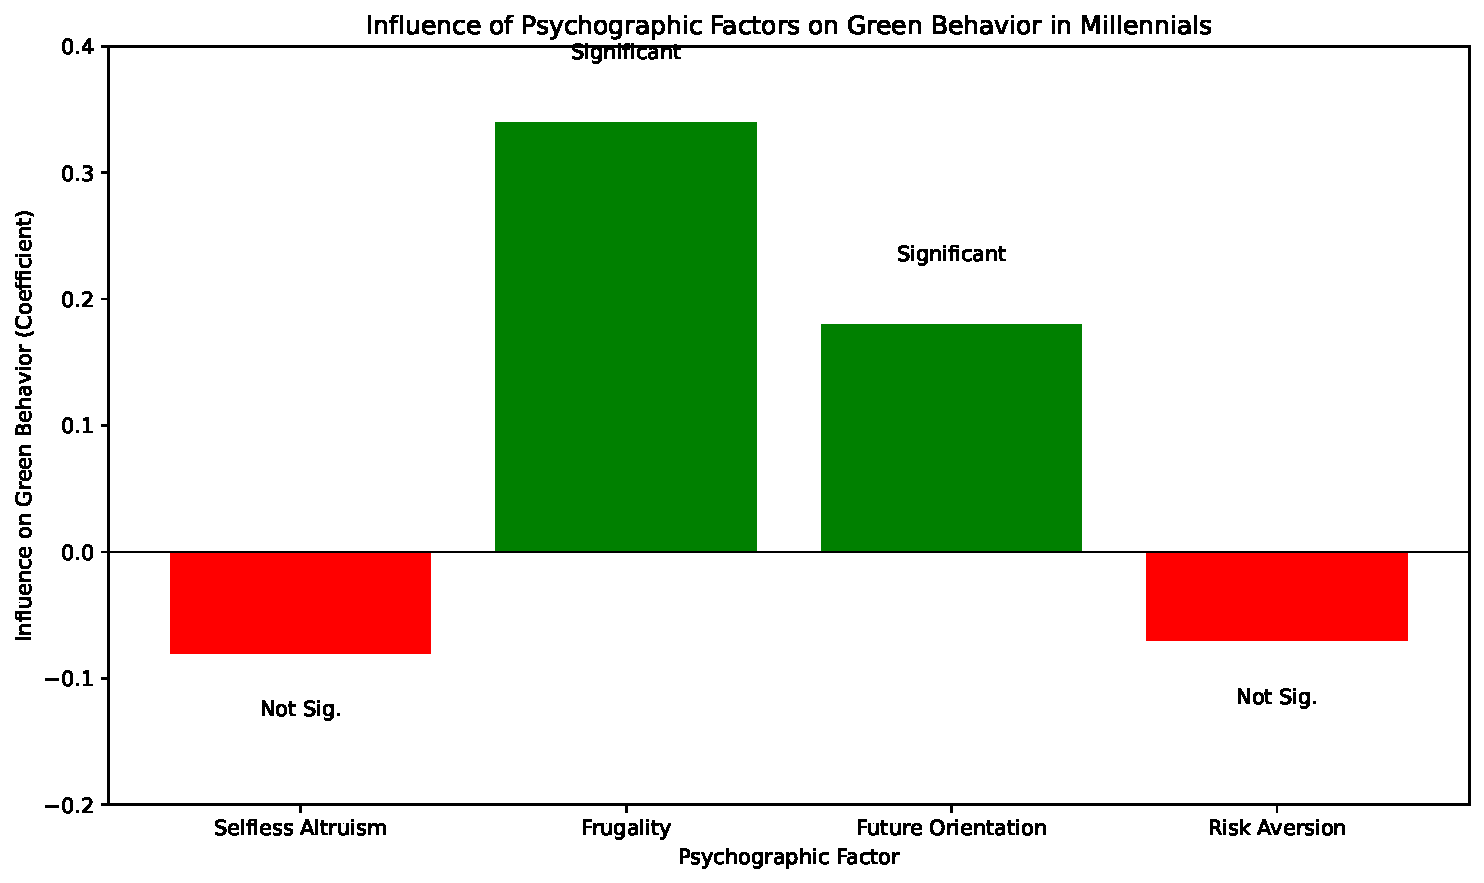
\includegraphics{_thesis_files/figure-pdf/cell-11-output-1.pdf}

\subsection{Online Shopping Trends in
Taiwan}\label{online-shopping-trends-in-taiwan}

\begin{itemize}
\tightlist
\item
  In Online Shopping, (聯合新聞網, 2024 predicts Momo and Coupang will
  compete for Taiwanese market leadership).
\item
  intsifying competition, Coupang stepping on Shopee's and MOMO's toes
  Anon (2024j)
\end{itemize}

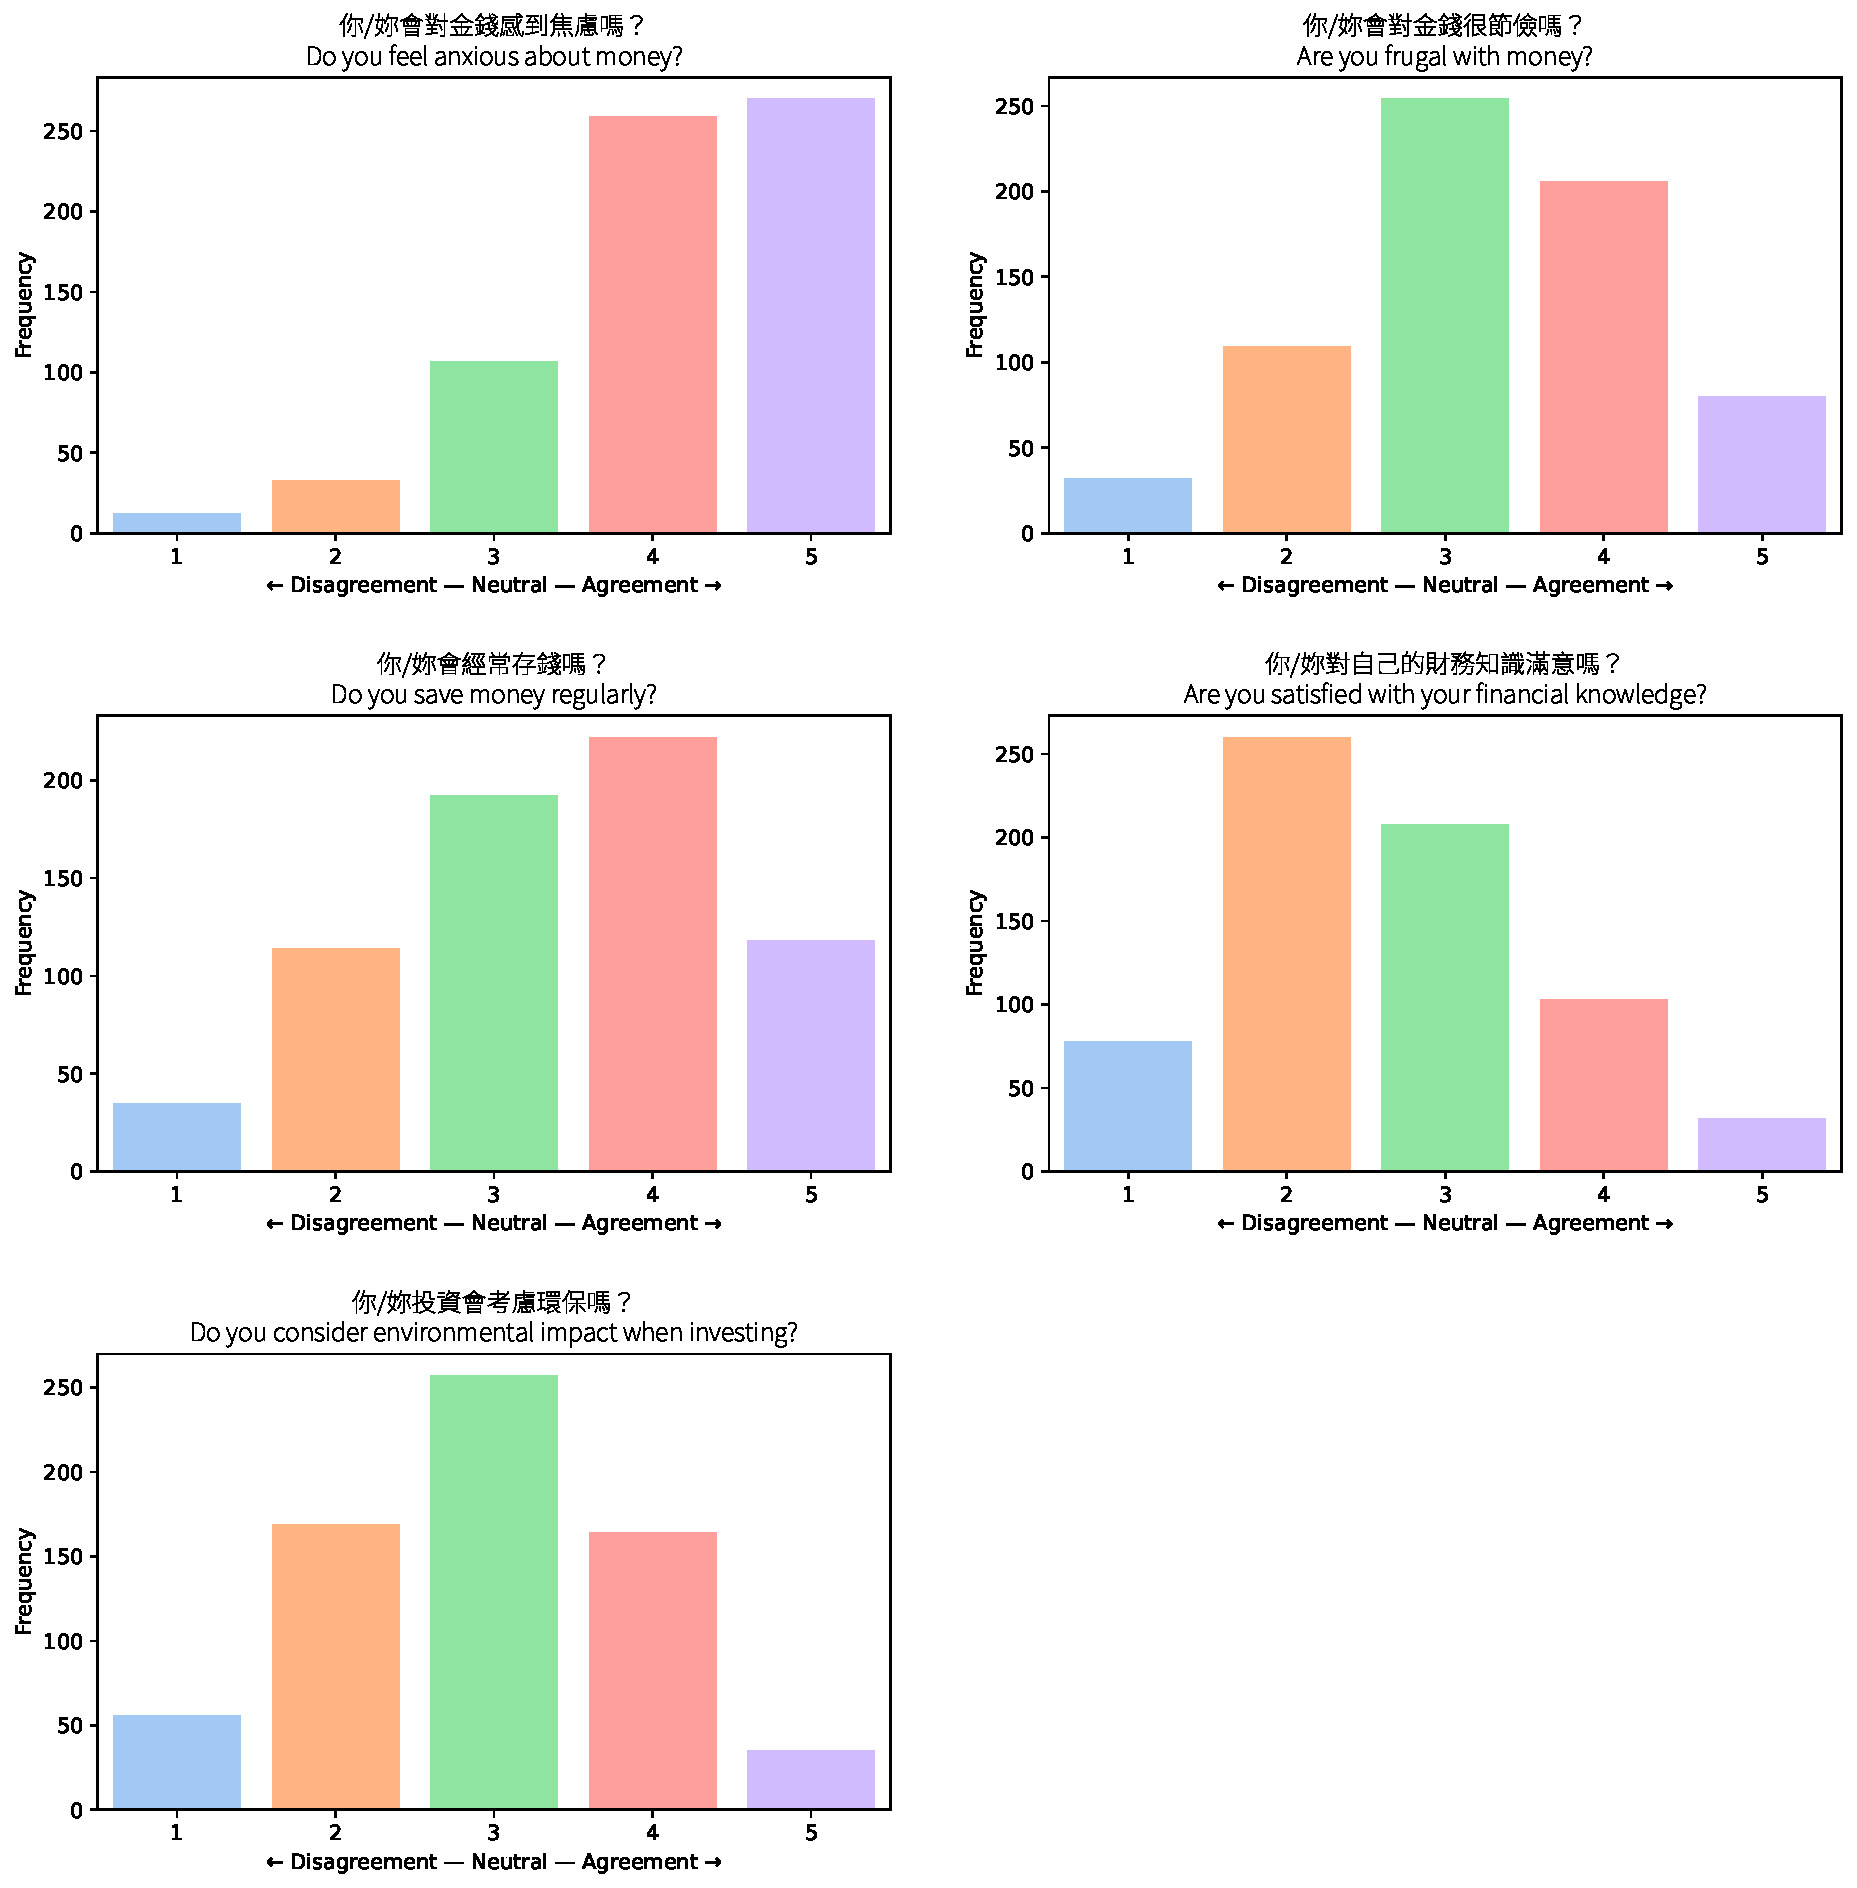
\includegraphics{_thesis_files/figure-pdf/cell-12-output-1.pdf}

\begin{itemize}
\tightlist
\item
  ``Taiwan's Financial Supervisory Commission's (FSC) requirements for
  Taiwan's corporates to disclose their carbon emissions starting in
  2023,'' Reformosatw (2024)
\end{itemize}

\subsubsection{Gen-Z in Other Countries}\label{gen-z-in-other-countries}

\begin{itemize}
\item
  In Japan, Gen-Z wants privacy and 75\% feel others overshare on social
  media and 49 percent were concerned about their personal data
  https://www.mckinsey.com/\textasciitilde/media/mckinsey/email/genz/2022/06/07/2022-06-07b.html
\item
  (Manchanda et al., 2023) survey (n=726) administered at shopping malls
  in New Delhi, India, found similar levels of sustainability
  consciousness between Millenial (n=206) and Generation-Z (n=360) age
  groups; people with high level of materialism were found to be less
  sustainability-conscious; the effect of mindfulness on sustainability
  was found to be stronger among females than males, supporting the
  hypothesis of the moderating effect of gender.
\end{itemize}

\textbf{There's evidence young people have money.} In the United States,
the combined annual consumer spending of Gen-Z and Millennials was over
2.5 Trillion USD in 2020 (YPulse, 2020). Over the decade from 2020 to
2030, in the U.S., UK, and Australia, Millennials are projected to
inherit 30 trillion USD from their parents (Calastone, 2020). There's
also some evidence of investment interest, however there's large
geographic variance. According to a (Calastone, 2020) study (n=3000)
surveying people in the millennial age group between ages 23 and 35 in
Europe (UK, France, Germany), U.S.A., Hong Kong, and Australia, 48\% of
respondents located in Hong Kong owned financial securities (such as
stocks) while the figure was just 10\% in France.

\begin{longtable}[]{@{}ll@{}}
\caption{From millennial investors (Calastone, 2020).}\tabularnewline
\toprule\noalign{}
Place of Comparison & Financial Security Ownership \\
\midrule\noalign{}
\endfirsthead
\toprule\noalign{}
Place of Comparison & Financial Security Ownership \\
\midrule\noalign{}
\endhead
\bottomrule\noalign{}
\endlastfoot
Hong Kong & 48\% \\
France & 10\% \\
& \\
\end{longtable}

There is extensive research on the attitudes of U.S. college students
towards climate change. (American Press Institute, 2022) reports only
37\% percent of U.S. Generation-Z and Millenials follow news related to
environmental issues. (Schwartz et al., 2022) reports some adult US
students in a small study (18-35, n = 284) express feelings of
insignificance of their actions to achieve any meaningful impact.
(Thomaes et al., 2023) reports U.S. adolescents don't find
sustainability relevant to their daily life. (Ross et al., 2016) says
most people in the U.S. don't act on climate change. ``Action on climate
change has been compromised by uncertainty, aspects of human
psychology''.

\begin{itemize}
\item
  In Portugal, Estonia, and elsewhere young people are suing companies
  for eco-problems: Flor (2024)
\item
  The En-ROADS climate change solutions simulator allows governments,
  organizations and individuals explore climate scenarios based on
  interactive changes in a visualization tool (Czaika \& Selin, 2017;
  Creutzig \& Kapmeier, 2020; Climate Interactive, 2023, n.d.).
\item
  ``Research shows that showing people research doesn't work,'' John
  Sterman
\end{itemize}

\subsection{Pollution Levels}\label{pollution-levels}

Taiwanese college students are subjected to high levels of pollution.
University campuses are somewhat healthier than other areas. There are
several decades of research on pollution levels in Taiwan, most with
very scary correlations to health.

\begin{itemize}
\tightlist
\item
  Taiwan air pollution, the worst (highest PM2.5 concentration) were
  found in Changhua (24.5 µg/m³), Tainan (20.9 µg/m³), and Pingtong
  (20.7 µg/m³) (Chang Hsiung-feng, Wu Che-hao \& Wu Kuan-hsien, 2024).
\end{itemize}

Religion plays a role in air pollution: Tang \& Pan (2014)

\subsection{Developing Personas for College
Students}\label{developing-personas-for-college-students}

User research makes extensive use of user \emph{personas} to represent a
group of people with similar attributes. Designers use personas to
\emph{articulate assumptions,} which, if used well, is useful for
\emph{user-centered design}, to create better products. Personas help to
reflect on what kind of \emph{biases} might exist in the design. Within
the larger cohort of college students several different personas could
be defined, for example grouping people by interests, knowledge, habits,
levels of anxiety, and other attributes.

There have been concerns about food safety in Taiwan.

Humans have a long list of cognitive biases, which a good design should
take into account.

Students ride bicycles and scooters. Many circular economy service such
as YouBike and transport sharing platforms like Uber are available.

Many students live in dorms and shared housing, meaning their impact per
square meter is low.

\begin{itemize}
\item
  Students in the Generation-Z age bracket (abbreviated as Gen-Z or
  Zoomers) are born between 1997 and 2012 (Branka Vuleta, 2023). Over
  98\% of Gen-Z owns a smartphone while only 80\% of the general world
  population does (Global Web Index, 2017; BankMyCell, 2022).
\item
  High levels of technology adoption worldwide
\item
  (Credit Suisse, 2022) suggests young consumers are more eco-friendly
  and drive the speed of change. Yet the Economist has ran a few
  anonymous articles calling gen-z green ideals into question (The
  Economist, 2023; Anon, 2023o).
\item
  Deyan Georgiev (2023a)
\item
  Alex Reice (2021)
\item
  (Wood, 2022) suggests in the U.S. Gen-Z is willing to pay 10\% more
  for ethically goods, spend 24\% more on sustainable products than
  Generation X and 75\% of Gen Z would prioritize sustainability over
  brand loyalty.
\end{itemize}

The above studies give foundation for creating a persona of a U.S.
College Student who doesn't follow environmental news and thinks climate
action doesn't make a difference. This doesn't necessarily mean this
group of people with similar ideas would deny climate change is
happening. Rather ``Climate Denier'' could be another persona, grouping
people into a cohort who thinks climate change is not real. Further
research would be needed to define relevant personas which have
meaningful predictive and generalizing power.

\begin{longtable}[]{@{}lll@{}}
\caption{College Student Personas}\tabularnewline
\toprule\noalign{}
Description & Name & Beliefs \\
\midrule\noalign{}
\endfirsthead
\toprule\noalign{}
Description & Name & Beliefs \\
\midrule\noalign{}
\endhead
\bottomrule\noalign{}
\endlastfoot
Climate Change Denier & Jake & Climate change doesn't exist. \\
& Alice & \\
& Sam & \\
\end{longtable}

\begin{itemize}
\tightlist
\item
  Crabb (2023)
\end{itemize}

Rooney-Varga et al. (2019) shows the effectiveness of \textbf{\emph{The
Climate Action Simulation}} in educating users about \textbf{success
scenarios}.

\subsubsection{Social Trust}\label{social-trust}

\begin{itemize}
\tightlist
\item
  When disaster hits we need high levels of social trust.
\end{itemize}

\subsubsection{Climate Anxiety}\label{climate-anxiety}

A large worldwide study (n=10000, age 16-25) by (Hickman et al., 2021)
provides evidence the youth is anxious about climate in Australia,
Brazil, Finland, France, India, Nigeria, Philippines, Portugal, the UK,
and the USA. Similarly, (Thompson, 2021) finds young people around the
world have climate anxiety. (Whitmarsh et al., 2022) shows worry about
the climate in the UK is generally widespread (over 40\% of the
respondents, n=1332), while climate anxiety is highest among young
people and is a possible motivator for climate action. Additionally,
(Ogunbode et al., 2022) finds climate anxiety in 32 countries and also
supports the idea that climate anxiety leads to climate activism.
(Thibodeau, 2022): ``In 2021, the BBC polled 1,000 people in Scotland to
understand the barriers to taking climate action. What they found was
even though many people were aware of actions needed to take to address
climate change, and had intentions to their behaviors didn't change.
This is a phenomenon called the intention-action gap.''

\begin{itemize}
\item
  (Osaka, 2023) argues \emph{doomerism} is an excuse for climate
  in-action. Hope is necessary for people to make changes in their
  habits (Marlon et al., 2019).
\item
  Designing for Health and Sustainability: Health and sustainability are
  intrinsically connected. (Kjaergard, Land \& Bransholm Pedersen, 2014)
  shows how ``understanding health and sustainability as a duality,
  health both creates conditions and is conditioned by sustainability,
  understood as economic, social and environmental sustainability, while
  on the other hand sustainability creates and is conditioned by human
  health''
\item
  Design for Human Rights (UNFCCC, 2023b){]} text refers to ``human
  right to a clean, healthy and sustainable environment''.
\item
  Refi podcast: ``people need agency''.
\item
  Martiskainen et al. (2020) (need access, ncku doesn't subscribe)
\item
  Seabrook (2020) (need access)
\item
  Older research on young adults (Millenials at the time) highlights how
  Millenials ``use Google as a reference point for ease of use and
  simplicity'' (Kate Moran, 2016).
\end{itemize}

Psychological factors influencing millenials to engage with
sustainability (Naderi \& Van Steenburg, 2018)

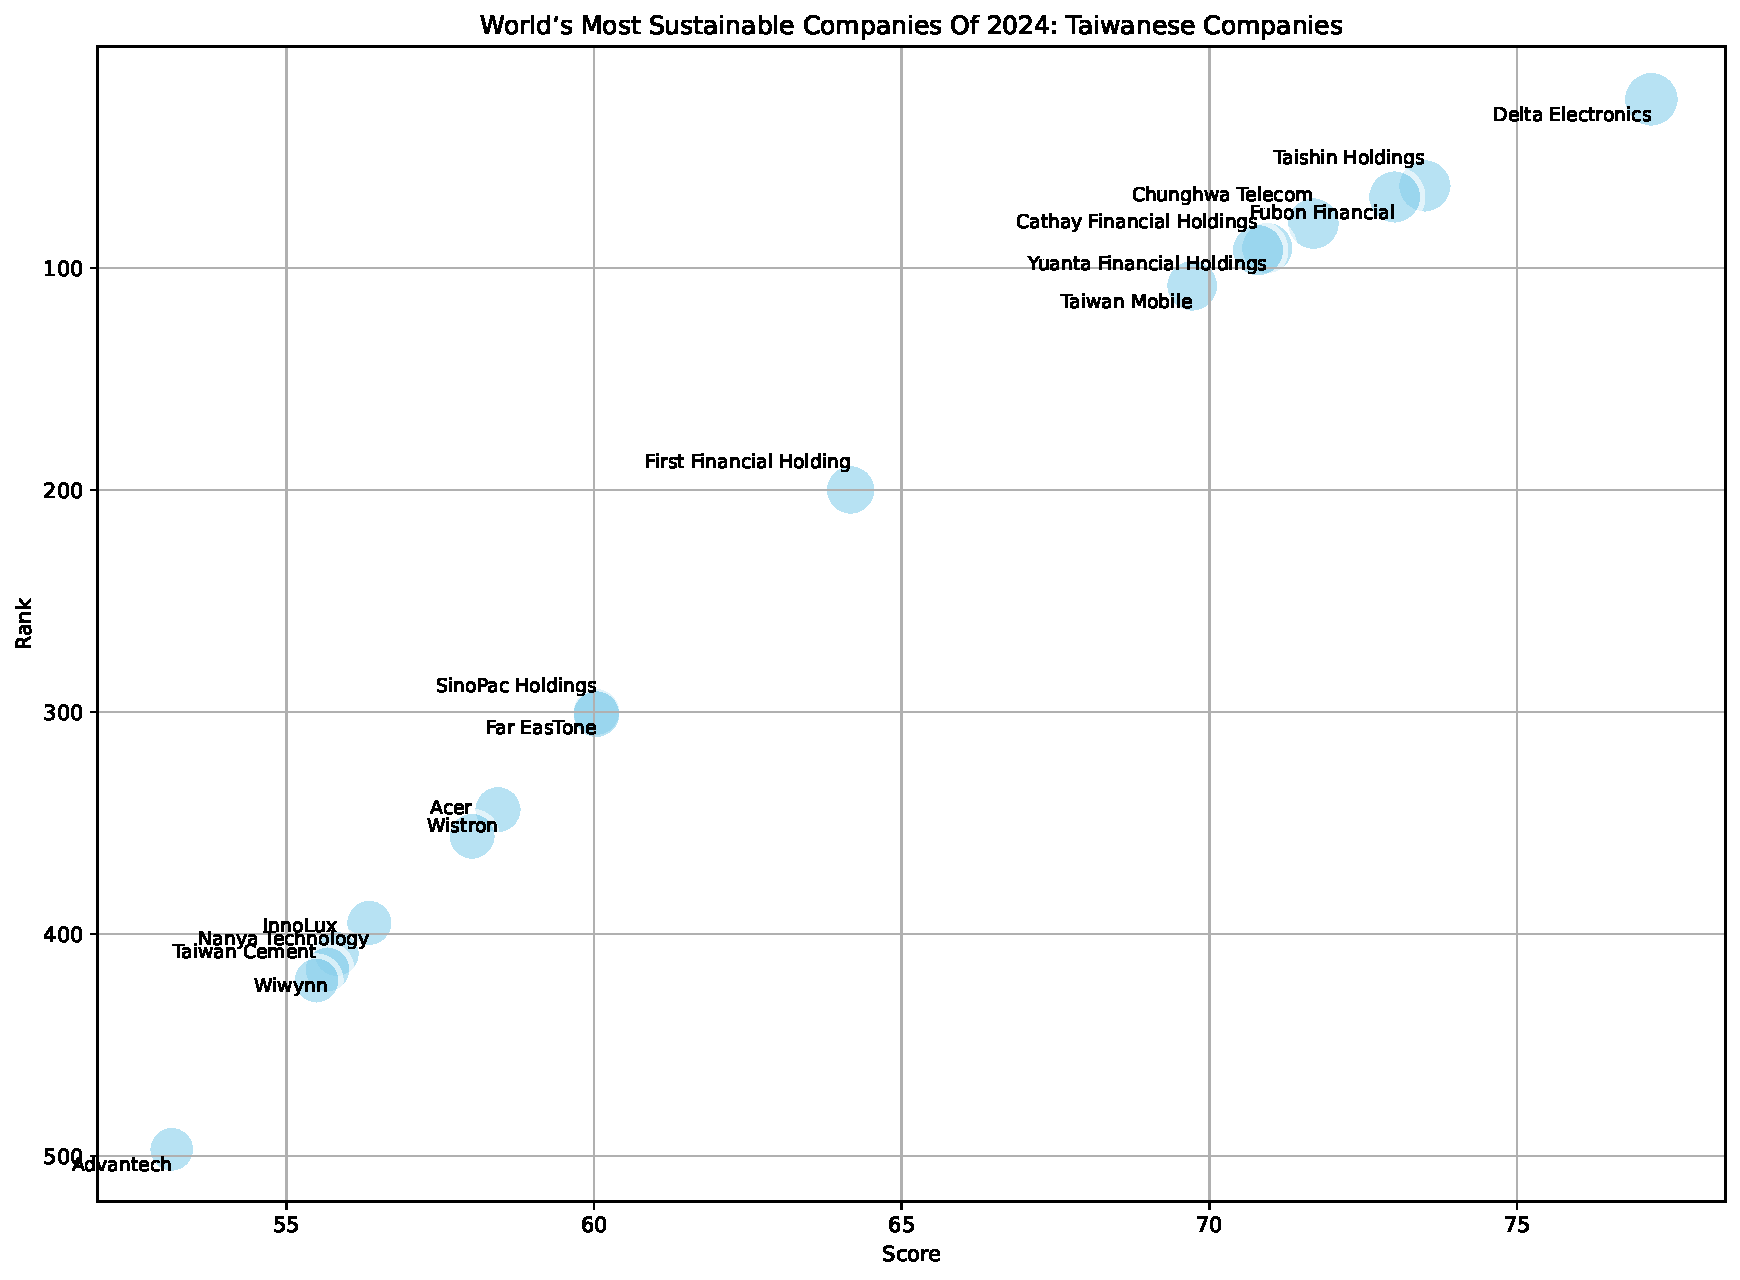
\includegraphics{_thesis_files/figure-pdf/cell-13-output-1.pdf}

\subsubsection{Community}\label{community}

Humans working together are able to achieve more than single
individuals. ``Any community on the internet should be able to come
together, with capital, and work towards any shared vision. That starts
with empowering creators and artists to create and own the culture
they're creating. In the long term this moves to internet communities
taking on societal endeavors.''

\begin{itemize}
\tightlist
\item
  Building a culture of sustainability? (Lakshmi Rebecca, 2018;
  Armstrong \& Staff, 2021).
\end{itemize}

The focus on \emph{group consciousness} suggests community-based
sustainability action may be effective.

\textbf{\emph{Zero Waste Lifestyle}} is the opposite of overconsumption.
Zero waste suggests people buy in bulk to save. Buying in bulk for more
savings and to reduce packaging. Through group purchases and community
investing while also reducing consumption. - Zero waste municipality in
Treviso

\textbf{\emph{Minimalism}} is a movement of people living a simple life.
This is always going to be a small percentage of people. (Costa, 2018):
Finnish socialists: minimalism. Tokyo (Tokyo Simple Eco Life, 2021). -
consumers choose to engage in becoming minimalist in a non-linear
process with overlapping stages (Oliveira De Mendonça, Coelho Rocha \&
Bogéa Da Costa Tayt-son, 2021).

What are the building blocks of a thriving community?

\textbf{\emph{Luxury}} - Conversely, Taiwan is a growing market for
luxury brands (Karatzas, Kapoulas \& Priporas, 2019).

\subsubsection{Empowerment}\label{empowerment}

\begin{itemize}
\tightlist
\item
  I would like to have an AI agent to set my requirements and
  preferences and give a ``fuck you'' middle finger to companies that
  don't meet them. I could also give a thumbs up to companies that meet
  my expectations. Perhaps the user interface could like Tinder where I
  can swipe left and right.
\end{itemize}

\subsubsection{Trends and Memes}\label{trends-and-memes}

\begin{itemize}
\item
  2024 ``underconsumption'' and ``deinfluencing'' are trends on TikTok
  Fares, Lee \& Lee (2024)
\item
  \url{https://www.tiktok.com/search?q=underconsumption}
\item
  \url{https://www.tiktok.com/search?q=deinfluence}
\item
  \url{https://www.tiktok.com/tag/deinfluencing}
\item
  \url{https://www.tiktok.com/tag/underconsumption}
\item
  Coined by Richard Dawkins in 1976 in the context of biology.
\item
  Internet memes and meme stocks
\item
  Memes from daily life, business to war, are relevant to penetrating
  through the noise of the web.
\item
  Memes and sustainability?
\item
  Meme research has become an academic discipline
\item
  Memes have become a popular communication tool..
\item
  Zidani (2021)
\item
  Zidani \& Miltner (2022)
\item
  Irina Lyan, Limor Shifman \& Sulafa Zidani (2015)
\item
  Zannettou et al. (2018)
\item
  Peters-Lazaro, Shresthova \& Jenkins (2020)
\end{itemize}

\subsection{Design Implications}\label{design-implications}

College Students Need Tools for Action

Environment shapes action.. create an environment where college students
can influence companies.

\begin{longtable}[]{@{}
  >{\raggedright\arraybackslash}p{(\columnwidth - 2\tabcolsep) * \real{0.0393}}
  >{\raggedright\arraybackslash}p{(\columnwidth - 2\tabcolsep) * \real{0.9607}}@{}}
\toprule\noalign{}
\begin{minipage}[b]{\linewidth}\raggedright
Category
\end{minipage} & \begin{minipage}[b]{\linewidth}\raggedright
Implication
\end{minipage} \\
\midrule\noalign{}
\endhead
\bottomrule\noalign{}
\endlastfoot
Community & Taiwanese students are influenced by the actions of their
peers; the app should show what other people are doing. \\
& People exist in relation to other people. \\
& Psychology of `fundraising clubs' vs individual investing \\
& Anon (n.d.bu) Ukraine DAO to support Ukraine through web3. \\
& These social movements are small and require too much effort to be
feasible for the app? Most college students are not zero waste or
minimalist. \\
& Group Purchases. \\
& Find Your Composting Community. \\
& Provides a community for pooling money with like-minded investors. \\
Climate Anxiety & How to support the youth? Design to reduce climate
anxiety? Is getting people to go to nature more a good way to increase
ecological awareness? Empowered by Design. Youth empowerment: The design
should empower young people. \\
& Consumer branded carbon credits like angry teenagers? \\
& Invest time not money, student don't have money? \\
Social Trust & \textbf{Show Success Scenarios!} \\
& Ask how much time you want to contribute. \\
& Match with other people based on time. \\
& Create a group chatroom. \\
& Use AI to help out with tips. \\
& Ask university students what do they study and match with that
industry to become expert and sustainability leader in this field. \\
& People want to help and make a difference. Give people things to do.
The Don't Look Up (n.d.) part of the \textbf{\emph{Don't Look Up}}
movie's social campaign provides 5 user models / roles for the audience
to follow: Consumer, Investor, Activist. \\
& Choose Your Climate Solutions. \\
& Younger people show higher motivation (participants in climate
protests). How to be relevant for a younger audience? \\
& Yet action remains low. \\
& Targeted and gated to college students. \\
& FB, etc, Gas all had the same launch strategy - start with students \\
& Kuzminski (2015) ecology of money \\
& Young people are mobile-first \\
& Persona: I care mostly about\ldots{} fashion, art, \ldots{} \\
& Young people like to follow trends. \\
& Food ordering apps are popular. \\
& Monoculture to regenerative food forests Oil to electric cars /
bicycles. \\
& Social Educational Edutainment Fun \\
& aespa (2020): Karina from Korea. It makes sense your sustainability
assistant would talk to you. Studies show gen N is speaking to computers
all the time. Interacting with the user is on the rise. For example,
Chime makes tipping suggestions on the place of purchase. \\
& The demographics that stand to win the most from the green
transformation of business are the youngest generations, with more years
of life ahead of them, and more exposure to future environmental and
social risks. It would be advisable for Generation Z and their parents
(Millennials) to invest their resources in greener assets, however, it's
still difficult to pick and choose between `good' and `bad' financial
vehicles to invest in. \\
& This creates an opportunity for a new generation of sustainable
investment apps, focusing on the usability and accessibility of ESG for
a mainstream audience. Generation Z and Millennials expect a
consumer-grade user experience. \\
& What would that experience look like? I've chosen these demographics
with the assumption that if given the right tools, the emotional demand
for sustainability could be transformed into action. The exploration of
systems of feedback to enable consumers to apply more direct positive
and negative pressure to the businesses and consumers signal
consequences for undesirable ecological performance is a major
motivation of this study. \\
\end{longtable}

\subsection{Feature Ideas}\label{feature-ideas}

\begin{longtable}[]{@{}
  >{\raggedright\arraybackslash}p{(\columnwidth - 2\tabcolsep) * \real{0.0383}}
  >{\raggedright\arraybackslash}p{(\columnwidth - 2\tabcolsep) * \real{0.9617}}@{}}
\toprule\noalign{}
\endhead
\bottomrule\noalign{}
\endlastfoot
& The current environmental upheaval, led by Gen-Z and Millennials, and
the business adaptation (or lack thereof) to sustainable economic
models, taking into account the hidden social and environmental costs we
didn't calculate in our pricing before. \\
& \begin{minipage}[t]{\linewidth}\raggedright
\begin{itemize}
\item
  We also need to consider environmental effects (E in ESG). We haven't
  taken into account the whole cost of production, leading to the wrong
  pricing information. To achieve this, we need expert governance (G).
\item
  I was unable to find similar research on university and post-graduate
  level students in Taiwan.
\item
  Taiwanese college students and SDGs (Ho et al., 2022).
\item
  College students in tourism and related fields . and sustainability
\item
  Consumers may be turned off by mentioning AI in product description.
  Cicek, Gursoy \& Lu (2024)
\item
  Progress in other areas of environmental protection has not made
  similar progress.
\item
  There are documentaries about oil product
\item
  Plastic production documentary
\item
  I've seen several.. find and cite them to show the progression of the
  environmental movement in Taiwan ADD CITATION
\item
  The Taiwanese Green party
\item
  Contact SOAS?
\end{itemize}
\end{minipage} \\
\end{longtable}

\newpage

\section{Sustainability}\label{sustainability}

\begin{figure}[H]

{\centering 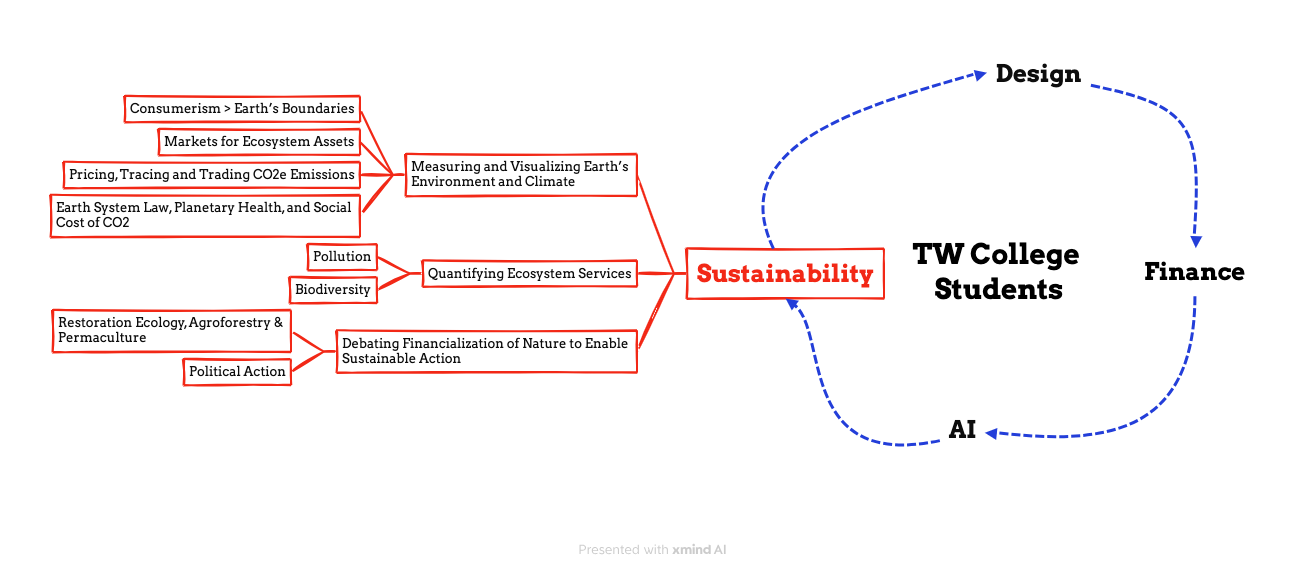
\includegraphics{./images/sustainability/abstract-sustainability.png}

}

\caption{Visual abstract for the sustainability chapter}

\end{figure}%

\subsection{The Roots of Sustainability in
Environmentalism}\label{the-roots-of-sustainability-in-environmentalism}

\emph{``Nachhaltigkeit''} - \emph{sustainability} in German - was likely
the first use of the concept of preserving natural resources, conceived
by a tax accountant Hannß Carl von Carlowitz in 1713 in his seminal book
on forestry - \emph{Sylvicultura oeconomica -}, referring to the goal of
achieving prudent forest management practices in his native Saxony in
Southeastern Germany, which at the time was under severe
\emph{deforestation} pressure from mining, ship-building and
agricultural production (Hannß Carl von Carlowitz, 1713; Gottschlich \&
Friedrich, 2014). This particular field of sustainability study is now
known as \emph{sustainable yield of natural capital}. The
\emph{principal} of the natural resource being managed, such as in
fishing and forestry, shouldn't be over-harvested in order to maintain
\textbf{\emph{ecosystem services}} - a contemporary term from the theory
of \emph{natural capital}, referring to benefits humans receive from the
stock of world's natural resources (Peter Kareiva et al., 2011).

Defining sustainability perhaps more poetically, the American wildlife
ecologist Aldo Leopold proposed the idea of \emph{land ethics} in 1972
as \emph{``{[}a{]} thing is right when it tends to preserve the
integrity, stability, and beauty of the biotic community. It is wrong
when it tends otherwise''} in his landmark work \emph{A Sand County
Almanac} (Leopold, 1972). In a similar vein, the 1987 United Nations'
Brundtland Report titled ``\emph{Our Common Future''} defined
\emph{sustainable development} as \emph{``Development that meets the
needs of the present without compromising the ability of future
generations to meet their own needs''} (Anon, 1987). Given these varied
ideas for over 300 years, I believe some percentage of people have been
concerned with our planet's natural environment and its preservation
already for centuries. Yet, it is only in the last 100 and so years that
human activities have begun to affect Earth's systems on a previously
unseen scale - termed \emph{Anthropocene} -, necessitating a deeper
understanding of human-nature interactions, such as in the case of
climate change, which is rapidly changing the face of our living
environments.

\subsection{Measuring, Visualizing Earth's
Climate}\label{measuring-visualizing-earths-climate}

Studies of Earth's climate go back for over 200 years, starting with
Alexander von Humboldt,the founder of climatology, who revolutionized
cartography by inventing the first \emph{isothermal maps} in 1816; these
maps showed areas with similar temperature, variations in altitude and
seasons in different colors (Honton, 2022) now available as 3D computer
models(Anon, 2023p). Already in 1896, the Nobel Prize winner Svante
Arrhenius first calculated how an increase in CO\textsubscript{2} levels
could have a warming effect on our global climate (Anderson, Hawkins \&
Jones, 2016; Wulff, 2020). In 1938, Guy Stewart Callendar was the first
scientist to demonstrate the warming of Earth's land surface as well as
linking the production of fossil fuels to increased CO\textsubscript{2}e
and changing climate (Hawkins \& Jones, 2013). Early scientists
pioneered climate modeling by calculating the first climate interactions
which precede today's complex computer-based \emph{Earth System Models
(ESMs)} that integrate the various Earth systems and cycles run on
supercomputers (Anderson, Hawkins \& Jones, 2016).

\begin{figure}[H]

{\centering 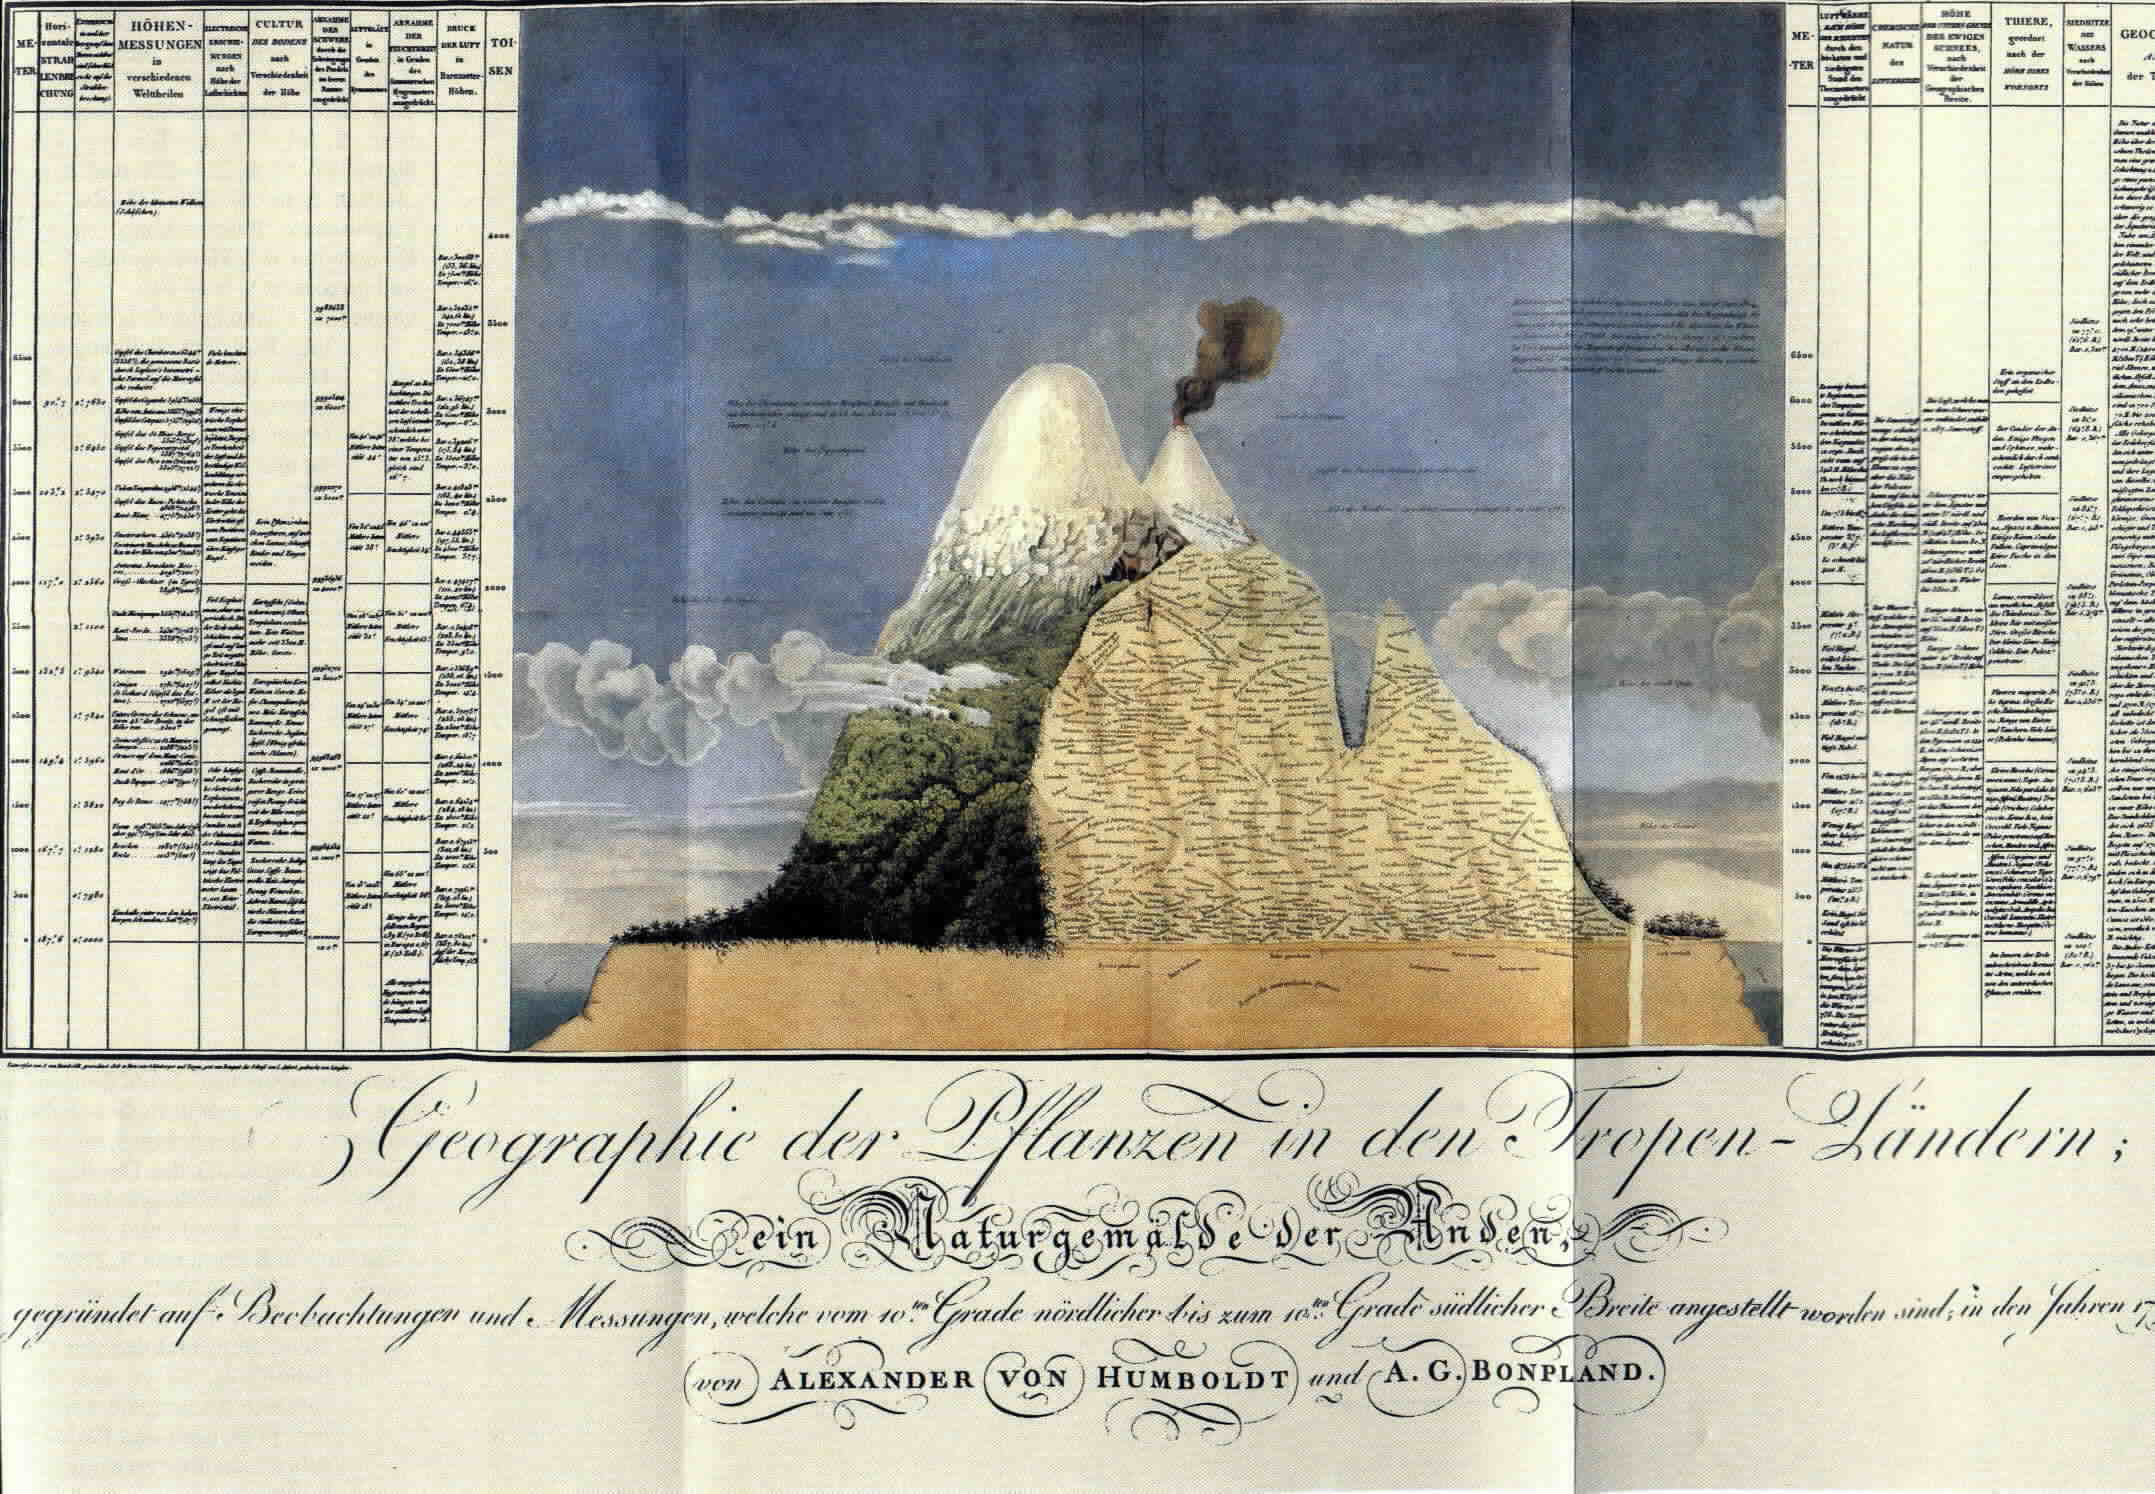
\includegraphics[width=1\textwidth,height=\textheight]{./images/sustainability/humboldt.jpg}

}

\caption{Humboldt's Naturgemälde, early data visualization of ecology,
rain, temperature, elevation, etc}

\end{figure}%

Environmental activists have been calling attention to global warming
for decades, yet the world has been slow to act (McKibben, 1989). While
the scientific case for human-induced climate change was building, it
took 120 years after Arrhenius' calculations, until the Paris Climate
Agreement in 2016, that countries came to an agreement on non-binding
targets on keeping CO\textsubscript{2} levels 1.5 °C below
pre-industrial levels (defined as 1850--1900)(United Nations, 2016).
Even though awareness of Earth's warming climate was growing ever
stronger, the CO\textsubscript{2} emissions kept rising too. The
hockey-stick growth of CO\textsubscript{2} concentration since the
industrial revolution is clear in the data from 1958 onward, following a
steady annual increase, called the \emph{Keeling Curve} (Keeling \&
Keeling, 2017). Written records of global temperature measurements are
available starting from the 1880s, when temperatures began to be
documented in ship logs (Brohan et al., 2012). Finally, although perhaps
less accurately, temperature estimations from tree-trunks allow some
comparisons with the climate as far back as 2000 years ago (Rubino et
al., 2019).

\begin{figure}[H]

{\centering 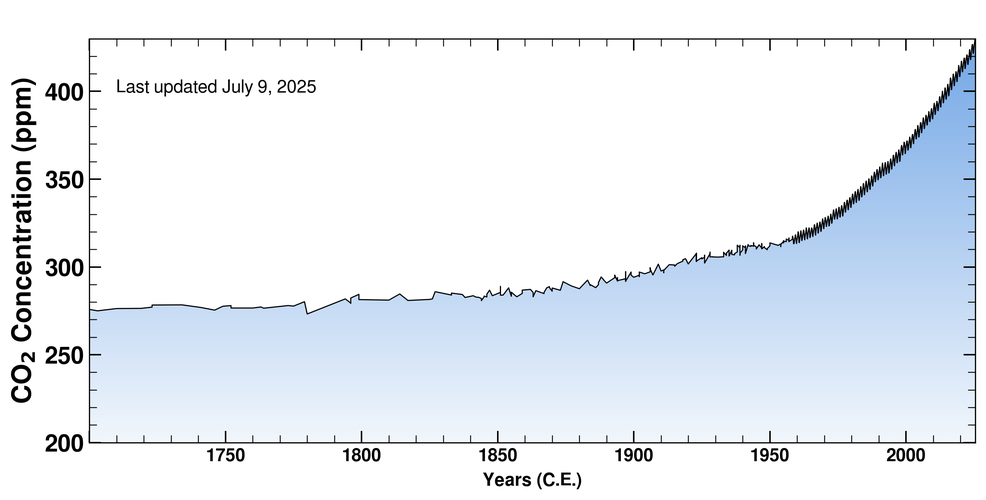
\includegraphics{./images/sustainability/co2-concentration.png}

}

\caption{CO\textsubscript{2} concentration in the atmosphere as of Ap.
Image Credit: Scripps Institution of Oceanography at UC San Diego.}

\end{figure}%

The latest data from 2023 shows our current world population of 8
Billion people emitted 37.2 gigatonnes (i.e.~billion metric tons) of
CO\textsubscript{2}e per year, the highest emissions recorded in history
(Statista, 2023a). In order to limit global warming to 1.5 °C as agreed
by the world nations in Paris, removal of 5-20 gigatons of
CO\textsubscript{2}e per year would be needed according to reduction
pathways calculated by the Intergovernmental Panel on Climate Change
(IPCC) (Wade et al., 2023). Yet, most countries are missing the mark
(Climate Analytics \& NewClimate Institute, 2023; United Nations
Environment Programme, 2023). The European Union's Copernicus Climate
Change Service (C3S) reports 1.5 °C global warming has already been
breached in 2024 temperatures (Anon, 2024i; Anon, 2024c). Given the
current pace of climate change action, the G7 countries (Canada, France,
Germany, Italy, Japan, United Kingdom, United States) are heading for
2.7 °C of warming by 2050 (CDP, 2022).

Earth's physical systems are very sensitive to small changes in
temperature, which was not understood until the 1970s(McKibben, 2006). A
comprehensive review of evidence from paleoclimate records until current
time, including ocean, atmosphere, and land surface of points towards
substantial climate change if high levels of greenhouse gas emissions
continue, termed by the authors as \emph{climate sensitivity} (Sherwood
et al., 2020). Global warming may lead to the slowing down and complete
stop of the Atlantic meridional overturning circulation (AMOC) which
helps maintain climate stability (Ditlevsen \& Ditlevsen, 2023).

\subsubsection{\texorpdfstring{Measuring CO\textsubscript{2}e
Emissions}{Measuring CO2e Emissions}}\label{measuring-co2e-emissions}

Technology improves and measurements have become more accurate yet
CO\textsubscript{2}e emissions are not yet completely accounted for.
(Crippa et al., 2020) reports the latest figures CO\textsubscript{2}e
from the EU's Emissions Database for Global Atmospheric Research
(EDGAR). The EU Copernicus satellite system reveals new greenhouse
emissions previously undetected (Daniel Värjö, 2022). \emph{Copernicus
Climate Change Service (C3S) provides ``{[}n{]}ear-real time updates of
key global climate variables}''(The Copernicus Climate Change Service,
2024).

\begin{itemize}
\tightlist
\item
  {[}@matthewgoreEmissionsRegulationsShipping2022{]} reports the
  International Maritime Organization (IMO) targets cutting
  CO\textsubscript{2} equivalent emissions in shipping 50\% by 2050
  compared to 2008.
\end{itemize}

Emissions production is highly unequal, with \emph{``{[}t{]}he world's
top 1\% of emitters produce over 1000 times more CO2 than the bottom
1\%''} (IEA, 2023a)

CO\textsubscript{2}e emissions by region (per year).

\begin{longtable}[]{@{}
  >{\raggedright\arraybackslash}p{(\columnwidth - 4\tabcolsep) * \real{0.3889}}
  >{\raggedright\arraybackslash}p{(\columnwidth - 4\tabcolsep) * \real{0.3194}}
  >{\raggedright\arraybackslash}p{(\columnwidth - 4\tabcolsep) * \real{0.2917}}@{}}
\caption{Comparing highest per capita CO\textsubscript{2e} emissions
(mostly from oil producers) vs regional average per capita
CO\textsubscript{2} emissions vs total CO\textsubscript{2}
emissions(Ivanova et al., 2020; World Resources Institute, 2020;
European Commission. Joint Research Centre., 2022; Crippa et al., 2020;
Liu et al., 2023d).}\tabularnewline
\toprule\noalign{}
\endfirsthead
\endhead
\bottomrule\noalign{}
\endlastfoot
\textbf{Regional Average Per Capita Emissions (2020)} & \textbf{Highest
Per Capita Emissions (2021)} & \textbf{Highest Total Emissions
(2021)} \\
North America 13.4 CO\textsubscript{2}e tonnes & Palau & China \\
Europe 7.5 CO\textsubscript{2}e tonnes & Qatar & United States \\
Global Average 4.1 CO\textsubscript{2}e tonnes & Kuwait & European
Union \\
Africa and the Middle East 1.7 CO\textsubscript{2}e tonnes & Bahrain &
India \\
& Trinidad and Tobago & Russia \\
& New Caledonia & Japan \\
& United Arab Emirates & Iran \\
& Gibraltar & Germany \\
& Falkland Islands & South Korea \\
& Oman & Indonesia \\
& Saudi Arabia & Saudi Arabia \\
& Brunei Darussalam & Canada \\
& Canada & Brazil \\
& Australia & Turkey \\
& United States & South Africa \\
\end{longtable}

\emph{Scoping} CO\textsubscript{2e} \emph{emissions} into 4 main
categories helps to organize calculating CO\textsubscript{2e} emissions
and corresponding reduction targets by looking at direct and indirect
emissions separately. The U.S. National Public Utilities Council (NPUC)
decarbonization report provides a useful categorization of
\emph{emission scopes} applicable to companies which helps organizing
emission reduction schemes (National Public Utilities Council, 2022)
based on the Greenhouse Gas Protocol defined in the 1990s (GHG Protocol,
n.d.). For example, for consumers in Australian states and territories
in 2018, 83\% of the GHG emissions are Scope 3, meaning indirect
emissions in the value chain (Goodwin et al., 2023). A newer concept is
Scope 4 emissions also known as avoided emissions, proposed by the World
Resources Institute (WRI) in 2013 (Plan A, n.d.).

\begin{longtable}[]{@{}ll@{}}
\caption{Definition of Emission Scopes From (National Public Utilities
Council, 2022).}\tabularnewline
\toprule\noalign{}
\endfirsthead
\endhead
\bottomrule\noalign{}
\endlastfoot
Emission Scope & Emission Source \\
Scope 1 & Direct emissions \\
Scope 2 & Indirect electricity emissions \\
Scope 3 & Value chain emissions \\
Scope 4 & Avoided emissions \\
\end{longtable}

One's scope 3 emissions are someone else's scope 1 emissions.

\begin{itemize}
\tightlist
\item
  Mapping pollution sources in China Xie et al. (2021)
\end{itemize}

Countries have agreed up CO\textsubscript{2e} Reduction Targets known as
Country-Level Nationally Determined Contributions (NDCs)

\begin{itemize}
\tightlist
\item
  UNFCCC. Secretariat (2022) The State of Nationally Determined
  Contributions
\end{itemize}

While most countries have not reached their Nationally Determined
Contributions, the Climate Action Tracker data portal allows to compare
countries (Climate Analytics \& NewClimate Institute, 2023). (Fransen et
al., 2022) notes that the majority of Nationally Determined
Contributions (NDCs) are dependent on financial assistance from the
international community.

\begin{longtable}[]{@{}ll@{}}
\caption{Climate Action Tracker's country comparison of the 10 top
polluters' climate action.}\tabularnewline
\toprule\noalign{}
\endfirsthead
\endhead
\bottomrule\noalign{}
\endlastfoot
Country or Region & NDC target \\
China & Highly insufficient \\
Indonesia & Highly insufficient \\
Russia & Critically insufficient \\
EU & Insufficient \\
USA & Insufficient \\
United Arab Emirates & Highly insufficient \\
Japan & Insufficient \\
South Korea & Highly insufficient \\
Iran & Critically insufficient \\
Saudi Arabia & Highly insufficient \\
\end{longtable}

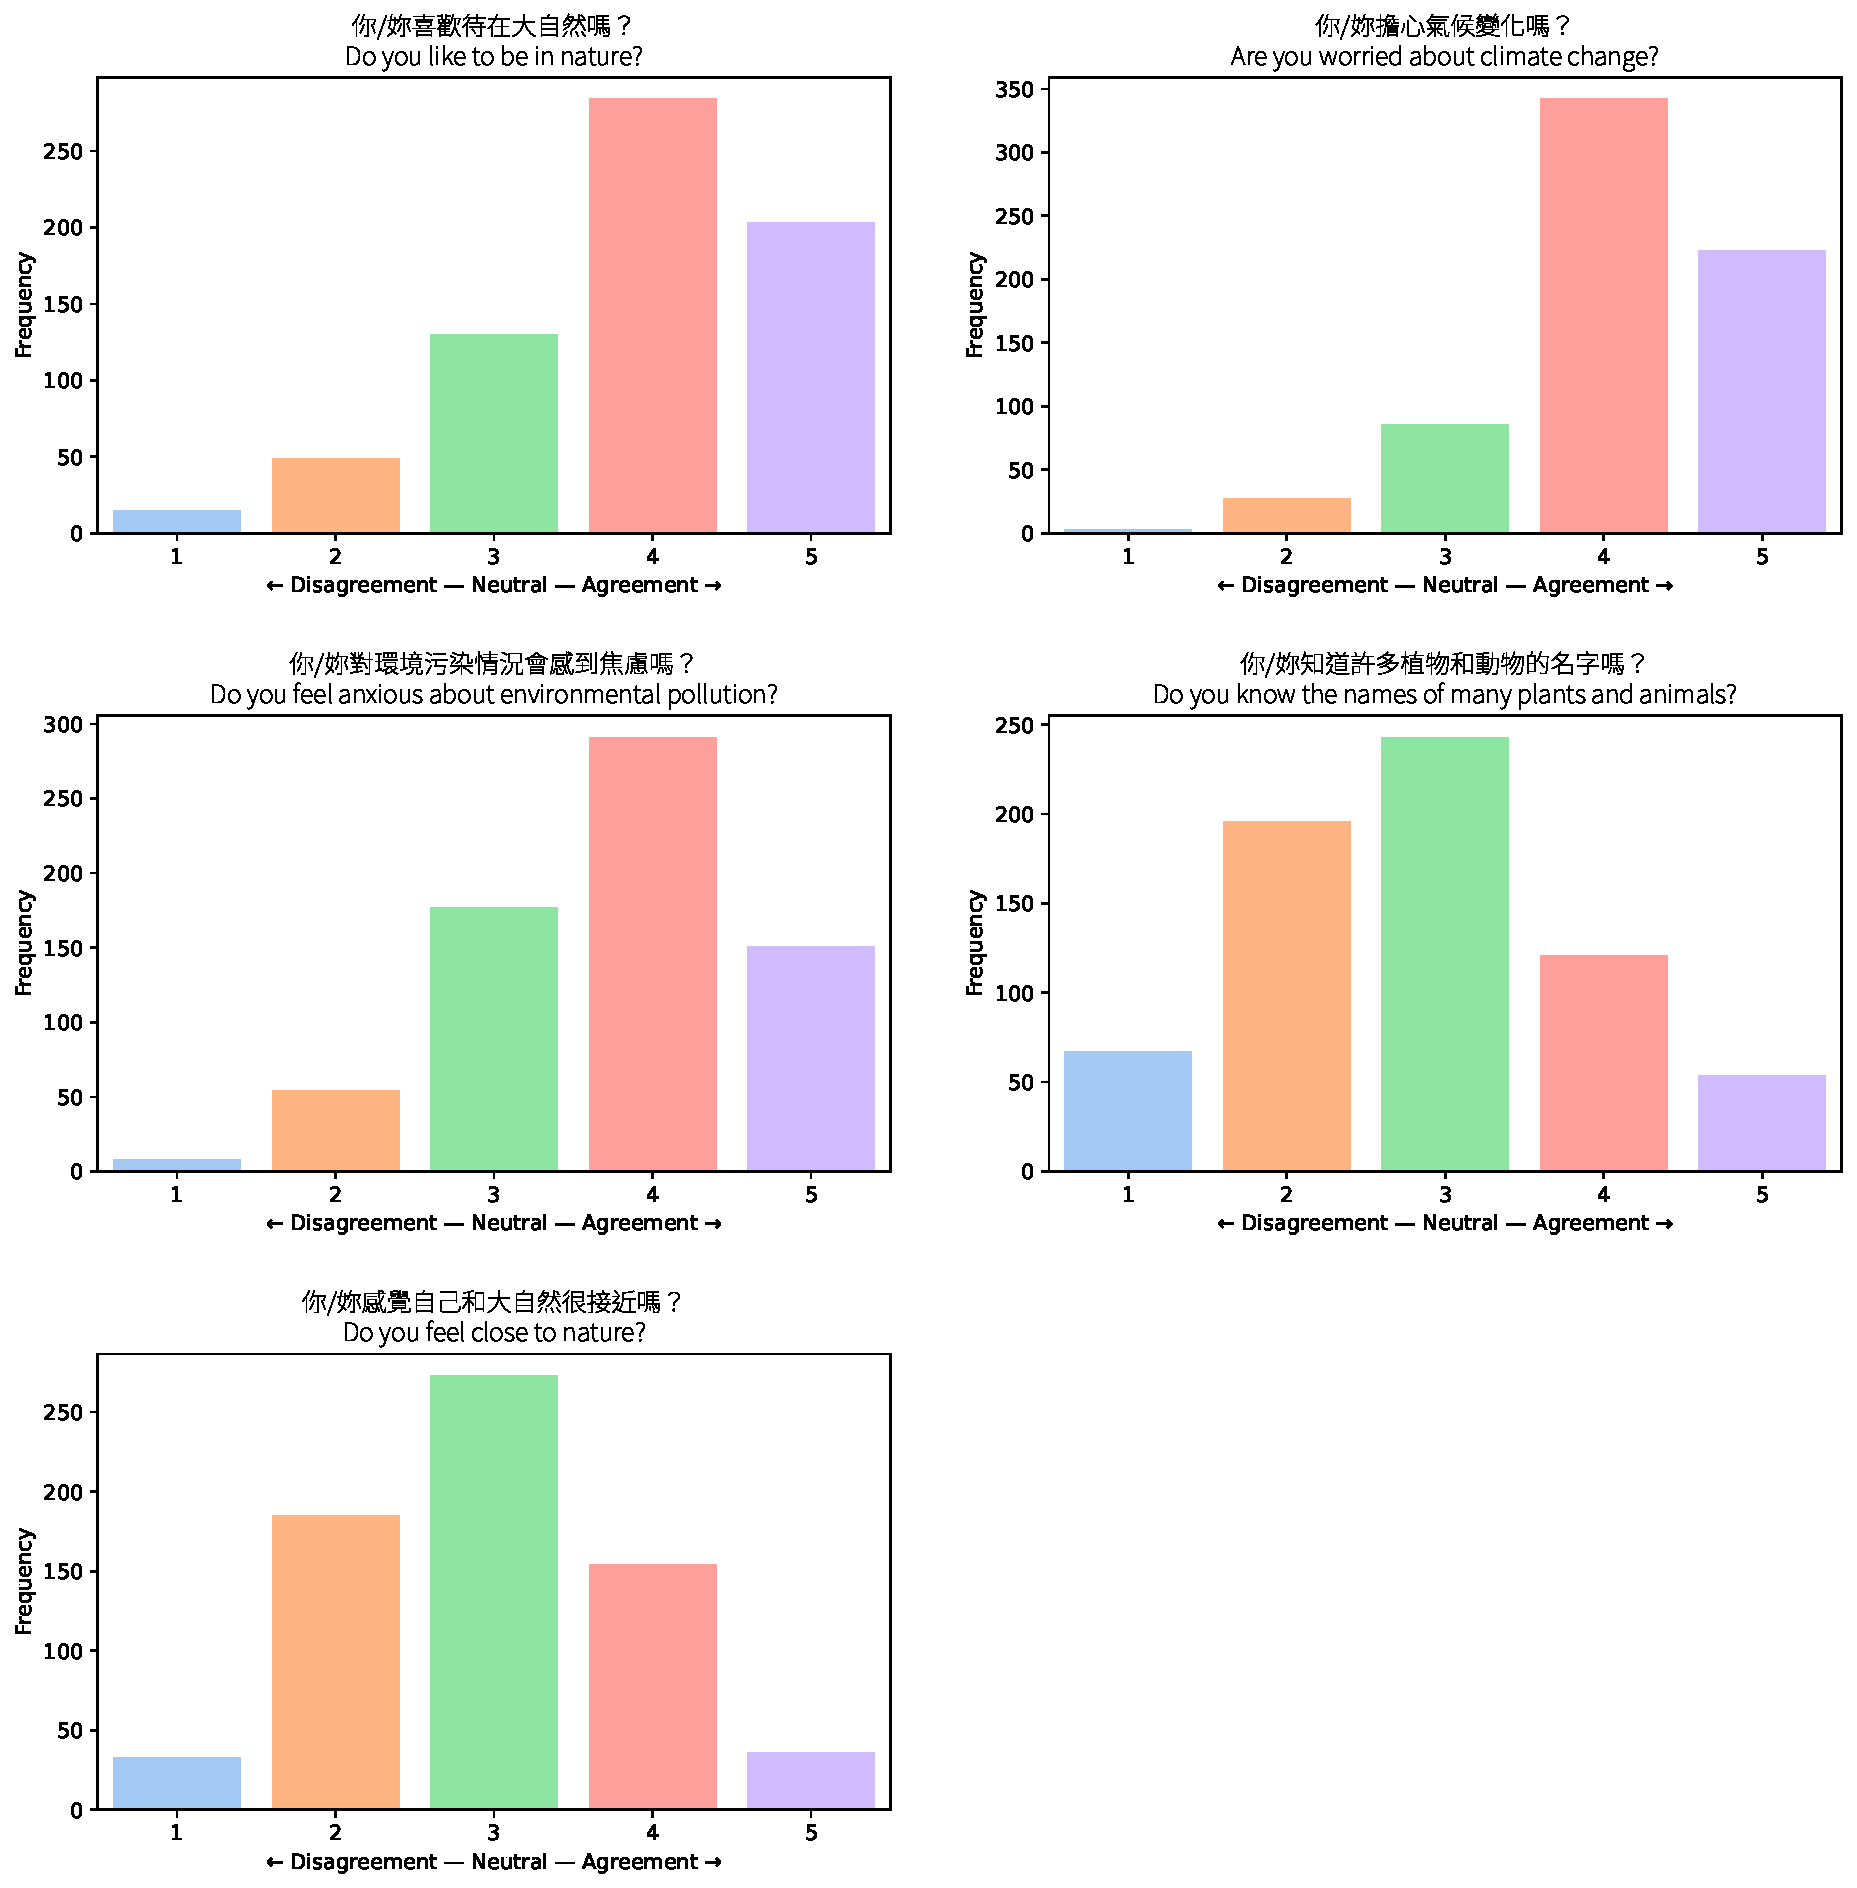
\includegraphics{_thesis_files/figure-pdf/cell-15-output-1.pdf}

Fossil fuels are what powers humanity as well as the largest source of
CO\textsubscript{2} emissions. IEA (2022) reports ``Global
CO\textsubscript{2} emissions from energy combustion and industrial
processes rebounded in 2021 to reach their highest ever annual level. A
6\% increase from 2020 pushed emissions to 36.3 gigatonnes''. As on June
2023, fossil fuel based energy makes up 82\% of energy and is still
growing Institute (2023). The 425 largest fossil fuel projects represent
a total of over 1 gigatons in CO\textsubscript{2} emissions, 40\% of
which were new projects Kühne et al. (2022). Tilsted et al. (2023)
expects the fossil fuel industry to continue grow even faster. In July
2023, the U.K. granted hundreds of new oil and gas of project licenses
in the North Sea (Anon, 2023ab).

\subsubsection{Markets for Ecosystem Assets: Pricing, Tracing and
Trading}\label{markets-for-ecosystem-assets-pricing-tracing-and-trading}

Markets for ecosystems assets are centered around \emph{carbon credits},
a type of nature-backed financial derivative dependent on science-based
methodologies for measurement, reporting, and verification (MRV), which
are managed and regularly updated by certification organizations such as
Gold Standard, Verra, and others.

\begin{longtable}[]{@{}
  >{\raggedright\arraybackslash}p{(\columnwidth - 2\tabcolsep) * \real{0.5000}}
  >{\raggedright\arraybackslash}p{(\columnwidth - 2\tabcolsep) * \real{0.5000}}@{}}
\caption{Criteria for carbon credit projects.}\tabularnewline
\toprule\noalign{}
\begin{minipage}[b]{\linewidth}\raggedright
Criteria
\end{minipage} & \begin{minipage}[b]{\linewidth}\raggedright
Description
\end{minipage} \\
\midrule\noalign{}
\endfirsthead
\toprule\noalign{}
\begin{minipage}[b]{\linewidth}\raggedright
Criteria
\end{minipage} & \begin{minipage}[b]{\linewidth}\raggedright
Description
\end{minipage} \\
\midrule\noalign{}
\endhead
\bottomrule\noalign{}
\endlastfoot
Baseline & Ecosystem carbon sequestration rate without the intervention
(project) \\
Additionality & New carbon capture or prevention of emissions \\
Permanence & Carbon storage time (should be long-term) \\
Leakage & Risk of shift to causing emissions (for example because of
deforestation) \\
\end{longtable}

Verra updated their Agricultural Land Management methodology for
Verified Carbon Standard (VCS) last year (Verra, 2023). Gold Standard
recently release a methodology for Mangrove-based carbon credits {[}ADD
CITATION{]}.

CO\textsubscript{2e} assigning a monetary value to carbon emissions.

Trading CO\textsubscript{2e} emissions can be divided into 2 categories
- \emph{Compliance Carbon Markets} (CCM) and \emph{Voluntary Carbon
Markets} (VCM).

The legislative baseline for Compliance Carbon Markets is so low, people
want to retire more CO\textsubscript{2e}, which they can do through
\emph{Voluntary Carbon Markets.}

For the individual person, there's no direct access to
CO\textsubscript{2} markets. However, brokers do buy large amounts of
carbon credits to resell in smaller quantities to retail investors.

\emph{``Carbon pricing is not there to punish people,''} says Lion Hirth
Lion Hirth (n.d.). \emph{``It's there to remind us, when we take travel,
heating, consumption decisions that the true cost of fossil fuels
comprises not only mining and processing, but also the damage done by
the CO\textsubscript{2} they release.''}

\emph{Long term cost} of insufficient climate action is more than
\emph{short-term gains} from delaying efforts to reduce carbon
emissions.

\begin{itemize}
\item
  The total size of carbon markets reached 949 billion USD in 2023,
  including Chinese, European, and North American CO\textsubscript{2}
  trading (LSEG \& Susanna Twidale, 02/12/2024, 02:37 PM).
\item
  \emph{The price of} CO\textsubscript{2e} \emph{differs across
  markets.} (Stern, 2022) argues carbon-neutral economy needs higher
  CO\textsubscript{2e} prices and believes (Rennert et al., 2022)
  CO\textsubscript{2e} price per ton should be 3,6x higher that it is
  currently. Contrary, (Ritz, 2022) argues optimal CO\textsubscript{2}
  prices could be highly asymmetric, low in some countries and high
  (above the social cost of CO\textsubscript{2e}) in countries where
  production is very polluting.
\item
  iGenius (2020)
\end{itemize}

The fossil energy production that's a large part of global CO2 emissions
has caused several high-profile pollution events. Large ones that got
international news coverage include Exxon Valdez and Deepwater Horizon.

\begin{itemize}
\tightlist
\item
  Lenton et al. (2023) quantifying human cost of global warming.
\item
\end{itemize}

CO\textsubscript{2e} credits has given rise to \emph{Carbon Accounting
industry.}

\begin{itemize}
\item
  Watershed is a large carbon accounting company.
\item
  The legislation has created an industry of CO\textsubscript{2}
  accounting with many companies like Greenly, Sustaxo, etc.
\item
  Quatrini (2021) sustainability assessments are complex and may give
  flawed results.
\item
  Nonetheles, CO\textsubscript{2} emission reduction has the added
  positive effect of boosting corporate morale (Cao, Li \& Hasan, 2023).
\end{itemize}

Compliance Carbon Markets

meet legal emission reduction targets

\textbf{Cap \& Trade}

The share of CO\textsubscript{2} emissions among people around the world
is highly unequal across the world (referred to as \textbf{\emph{Carbon
Inequality}}). (Chancel, 2022) reports ``one-tenth of the global
population is responsible for nearly half of all emissions, half of the
population emits less than 12\%''.

\begin{itemize}
\item
  One example is the ICT sector.
\item
  Bajarin (n.d.) Over 300 million PCs sold in 2022

  \begin{itemize}
  \tightlist
  \item
    Anon (2021h) Estonian company ``sustainable lifecycle management of
    IT equipment''
  \item
    Ärileht (23.09.2022, 12:53) Recycle your phone, FoxWay and Circular
    economy for PCs.
  \item
    Zhou et al. (2022a) ICT is an example of inequality, while emerging
    economies bear 82\% of the emissions, developed countries gain 58\%
    of value.
  \end{itemize}
\end{itemize}

\textbf{Emissions Trading Schemes}

From Carbon Offsets to Carbon Credits

\begin{itemize}
\tightlist
\item
  ``A carbon credit represents one tonne of carbon dioxide that has been
  prevented from entering or has been removed from the atmosphere''
  (Anna Watson, 2023, 2022).
\end{itemize}

Retiring CO\textsubscript{2} allowances

\begin{itemize}
\tightlist
\item
  Facilitating citizens' access to CO\textsubscript{2} emissions trading
  may be an efficient method to organize large-scale CO\textsubscript{2}
  retiring (Rousse, 2008).
\end{itemize}

As of 2024 there's no single global CO\textsubscript{2} trading market
but rather several local markets as described in the table below.

\begin{longtable}[]{@{}
  >{\raggedright\arraybackslash}p{(\columnwidth - 4\tabcolsep) * \real{0.2639}}
  >{\raggedright\arraybackslash}p{(\columnwidth - 4\tabcolsep) * \real{0.2639}}
  >{\raggedright\arraybackslash}p{(\columnwidth - 4\tabcolsep) * \real{0.4722}}@{}}
\caption{CO\textsubscript{2} credit trading markets around the world
from Anon (n.d.ak).}\tabularnewline
\toprule\noalign{}
\endfirsthead
\endhead
\bottomrule\noalign{}
\endlastfoot
CO\textsubscript{2} Market & Launch Date & Comments \\
EU & 2005 & EU: Araújo et al. (2020) \\
South Korea & 2015 & \\
China & 2021 & China's national emissions trading scheme (ETS) started
in 2021 priced at 48 yuan per tonne of CO\textsubscript{2}, averaged at
58 yuan in 2022 (Liu, 2021; Ivy Yin, 2023). \\
U.S. & 2013 & No country-wide market; local CO\textsubscript{2} markets
in California, Connecticut, Delaware, Maine, Maryland, Massachusetts,
New Hampshire, New York, Rhode Island, and Vermont \\
New Zealand & 2008 & New Zealand Rontard \& Reyes Hernández (2022) (need
access, important ncku doesn't subscribe) \\
Canada & 2013 & \\
\end{longtable}

Most of the world is not part of a CO\textsubscript{2} market.

\begin{itemize}
\item
  (Sipthorpe et al., 2022) compares traditional and blockchain-based
  solutions to carbon trading.
\item
  ``Blockchain solutions for carbon markets are nearing maturity'' and
  offer many improvements. enhancing transparency, trust, and
  efficiency.
\item
  (United Nations Environment Programme (UNEP), 2021) report. ``The
  Emissions Gap Report (EGR) 2021: The Heat Is On shows that new
  national climate pledges combined with other mitigation measures put
  the world on track for a global temperature rise of 2.7°C by the end
  of the century. That is well above the goals of the Paris climate
  agreement and would lead to catastrophic changes in the Earth's
  climate. To keep global warming below 1.5°C this century, the
  aspirational goal of the Paris Agreement, the world needs to halve
  annual greenhouse gas emissions in the next eight years.
\item
  (United Nations Environment Programme (UNEP), 2021) report ``If
  implemented effectively, net-zero emissions pledges could limit
  warming to 2.2°C, closer to the well-below 2°C goal of the Paris
  Agreement. However, many national climate plans delay action until
  after 2030. The reduction of methane emissions from the fossil fuel,
  waste and agriculture sectors could help close the emissions gap and
  reduce warming in the short term, the report finds. Carbon markets
  could also help slash emissions. But that would only happen if rules
  are clearly defined and target actual reductions in emissions, while
  being supported by arrangements to track progress and provide
  transparency.''
\item
  (United Nations Environment Programme, 2022) 2022 Emissions Gap
  report.
\end{itemize}

\begin{longtable}[]{@{}ll@{}}
\caption{Compliance market CO\textsubscript{2} prices on August 12,
2023; data from (Ember, 2023; Trading Economics, 2023; CarbonCredits,
2023).}\tabularnewline
\toprule\noalign{}
\endfirsthead
\endhead
\bottomrule\noalign{}
\endlastfoot
Compliance Markets & Price (Tonne of CO\textsubscript{2}) \\
EU & 83 EUR \\
UK & 40 Pounds \\
US (California) & 29 USD \\
Australia & 32 USD \\
New Zealand & 50 USD \\
South Korea & 5.84 USD \\
China & 8.29 USD \\
& \\
\end{longtable}

\begin{itemize}
\tightlist
\item
  tree bark absorbs methane, (Gauci et al., 2024).
\end{itemize}

Voluntary Carbon Markets

Verified Carbon Standard (VCS) and the Gold Standard, Climate Action
Reserve (CAR)‍, American Carbon Registry (ACR)

``BeZero Carbon is a ratings agency for the Voluntary Carbon Market.''

https://bezerocarbonmarkets.com/

Voluntary Carbon Markets are \ldots{}

Voluntary Carbon Markets (VCM) lack standardization and transparency
(Ela Khodai, 2023).

\emph{Carbon Credits} are useful for private companies who wish to claim
\emph{carbon neutrality, climate positivity}, or other related claim,
which might be viewed in good light by their clients or allow the
companies to adhere to certain legislative requirements.

There are many companies which facilitate buy carbon credits as well as
a few organizations focused on carbon credit verification.

\begin{itemize}
\tightlist
\item
  In Estonia, startups Arbonic and Single.Earth are trialing this
  approach in several forests.
\item
  For example Flickr invested 3000 USD in carbon credits and got a
  carbon-neutral rating (?!).
\item
  Carbon Credit Retirement?
\item
  Methodologies: Anon (2022i)
\item
  KlimaDAO (2023) call for an open standard
\end{itemize}

\begin{longtable}[]{@{}ll@{}}
\caption{Voluntary market CO\textsubscript{2} prices on August 12, 2023;
data from (CarbonCredits, 2023).}\tabularnewline
\toprule\noalign{}
\endfirsthead
\endhead
\bottomrule\noalign{}
\endlastfoot
Voluntary Markets & Price (Tonne of CO\textsubscript{2}) \\
Aviation Industry Offset & \$0.93 \\
Nature Based Offset & \$1.80 \\
Tech Based Offset & \$0.77 \\
\end{longtable}

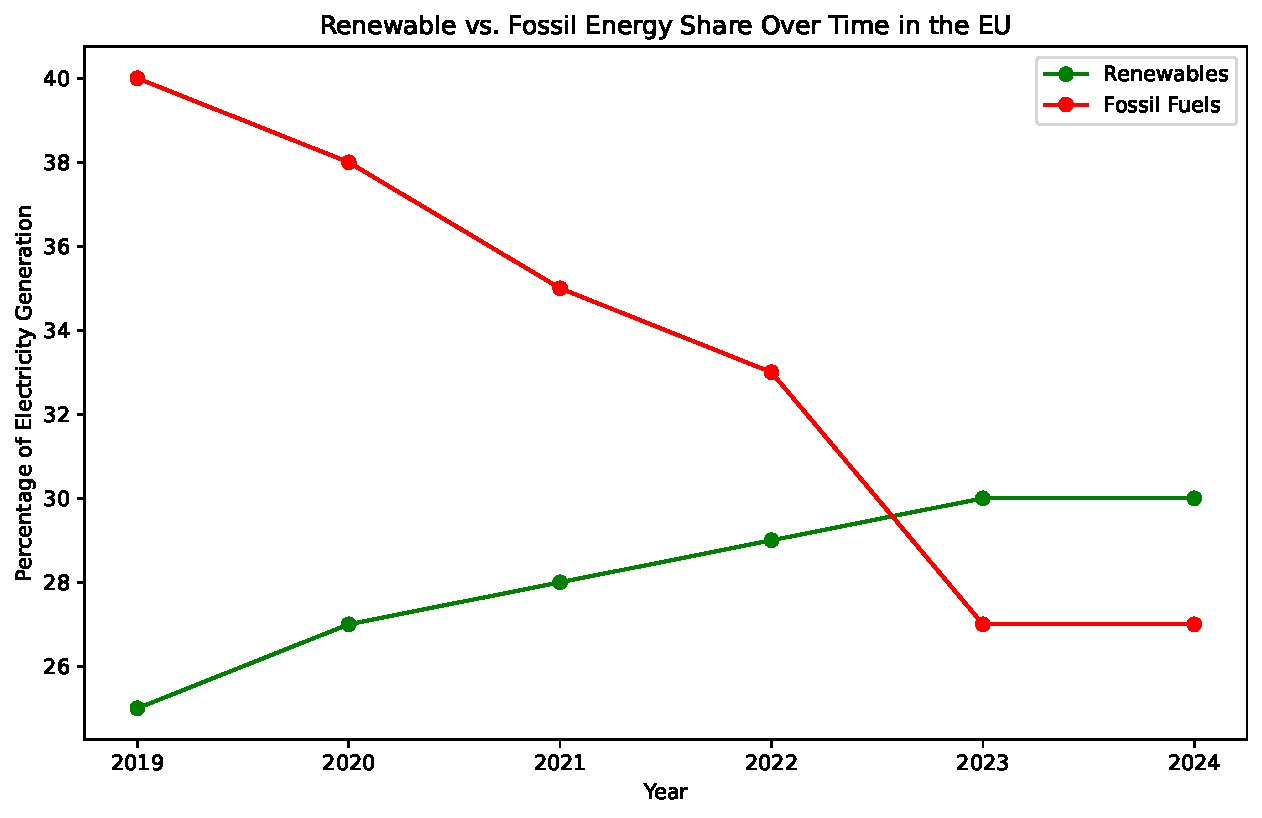
\includegraphics{_thesis_files/figure-pdf/cell-16-output-1.pdf}

\subsubsection{Overconsumption \textgreater{} Earth's
Boundaries}\label{overconsumption-earths-boundaries}

Excessive consumer lifestyle - \emph{overconsumption} - is one of the
main drivers of climate change and environmental destruction, with
\emph{``2/3 of global GHG emissions are directly and indirectly linked
to household consumption, with a global average of about 6 tonnes
CO\textsubscript{2} equivalent per capita''} , according to (Renee Cho,
2020; Ivanova et al., 2020). An older study put the number as high as
60\% percent (Ivanova et al., 2016) while (Ellen MacArthur Foundation,
Material Economics, 2019)'s models 45\% show of CO\textsubscript{2}
equivalent emissions come from our shopping; produced by companies to
make the products we consume.

With the trend of urbanization, it's not surprising (people living in)
cities are responsible for 80\% of the emissions (Rosales Carreón \&
Worrell, 2018). (Moberg et al., 2019) reports daily human activities
emission contribution on average in four European countries (France,
Germany, Norway and Sweden).

\begin{longtable}[]{@{}ll@{}}
\caption{Daily human activities emission contribution on average in
France, Germany, Norway and Sweden from (Moberg et al.,
2019).}\tabularnewline
\toprule\noalign{}
\endfirsthead
\endhead
\bottomrule\noalign{}
\endlastfoot
Emission Share & Category \\
21\% & Housing \\
30\% & Food \\
34\% & Mobility \\
15\% & Other \\
\end{longtable}

Earth's growing population reached 8 Billion people In November 2022 and
population projections by predict 8.5B people by 2030 and 9.7B by 2050
(The Economic Times, 2022; United Nations Department of Economic and
Social Affairs, Population Division, 2022). Indeed, making
\emph{anything} consumes natural resources, which are limited on planet
Earth. (Hassoun et al., 2023) forecasts increase of global food demand
by 62\% driven by the impact of climate change. Yet, while population
growth puts higher pressure on Earth's resources, some researchers
propose the effect is higher from wasteful lifestyles than the raw
number of people (Cardinale et al., 2012). Meanwhile others, such as
(Cafaro, Hansson \& Götmark, 2022), believe \emph{{[}o{]}verpopulation
is a major cause of biodiversity loss and smaller human populations are
necessary to preserve what is left.''}

While the numbers on overconsumption are clear, the debate on
overconsumption is so polarized, it's difficult to have a meaningful
discussion of the topic (Ianole \& Cornescu, 2013). Environmental risks
from human activities are known as Anthropogenic Threat Complexes (ATCs)
(Bowler et al., 2020)\emph{.} As long as humanity is a mono-planetary
species, we have to come to terms with the limitations of our home,
Earth.

\paragraph{Plastic Pollution}\label{plastic-pollution}

Overconsumption is also one of the root causes of plastic pollution.
(Ford et al., 2022) and (Lavers, Bond \& Rolsky, 2022) find strong links
between climate change and marine plastic pollution \emph{``along with
other stressors that threaten the resilience of species and habitats
sensitive to both climate change and plastic pollution''}.

Plastic pollution is pervasive around the Earth and is fundamentally
linked to climate change, while microplastics are increasingly a real
concern (Tiernan et al., 2022; Lavers, Bond \& Rolsky, 2022). Several
international studies report recent findings of microplastics everywhere
in human bodies: the brain, lungs, digestive tissues, bone marrow,
penis, testis, seminal fluid (semen), and placenta - causing serious
health and reproductive concerns (Main, 2024; Guo et al., 2024; Hu et
al., 2024; Codrington et al., 2024; Li et al., 2024; Montano et al.,
2023; Garcia et al., 2024; Zhu et al., 2024)

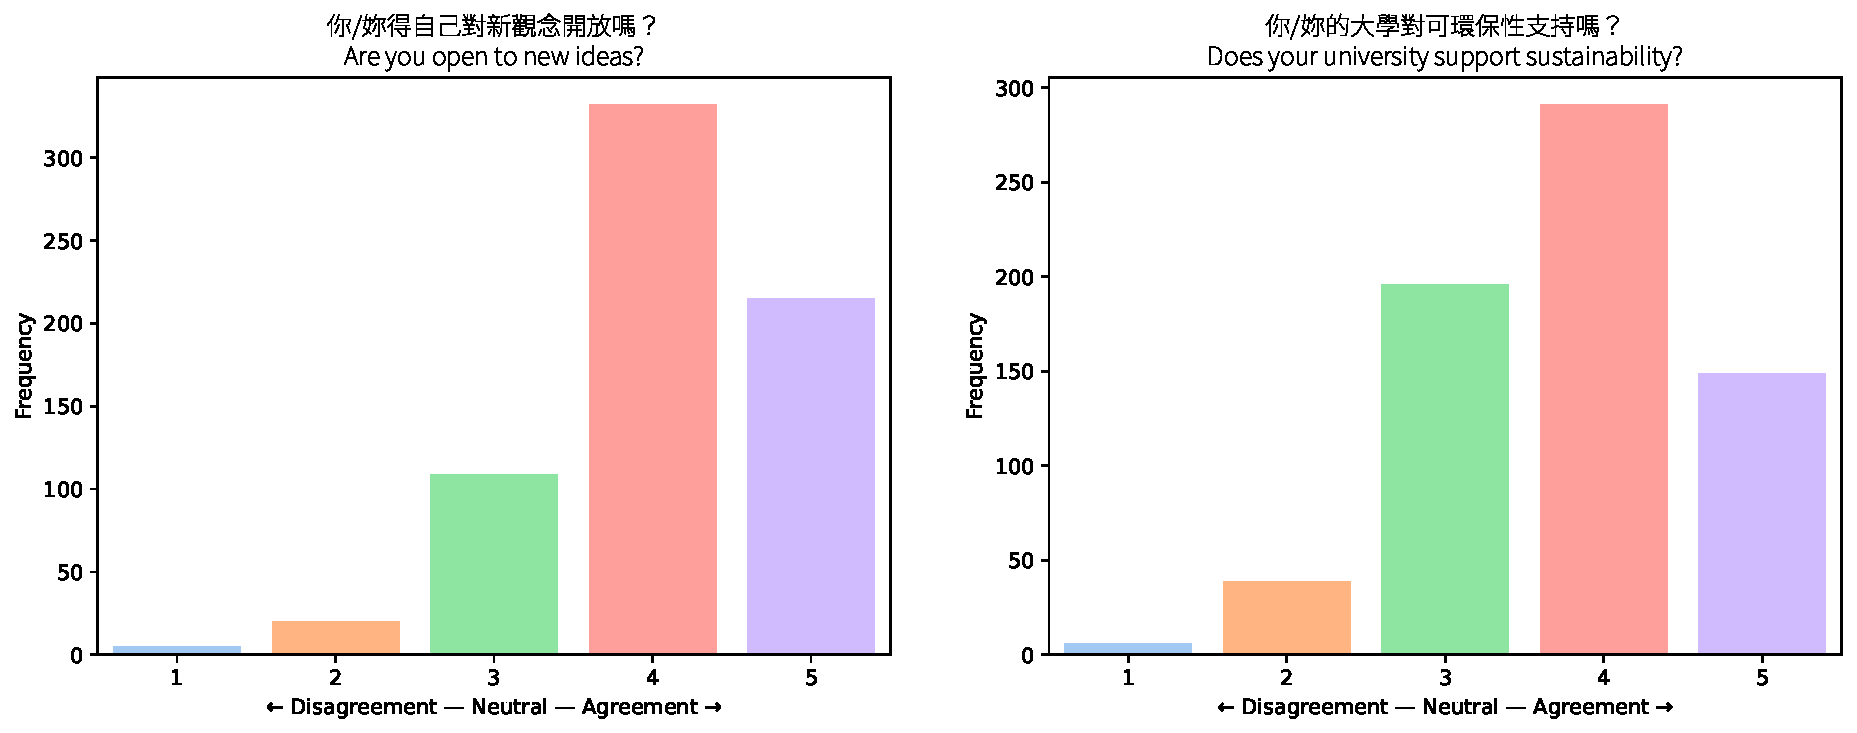
\includegraphics{_thesis_files/figure-pdf/cell-17-output-1.pdf}

\begin{itemize}
\tightlist
\item
  Jackson (2017) limits to growth update
\item
  (Keeble, 1988) reported in April 1987 that \emph{`residents in
  high-income countries lead lifestyles incompatible with planetary
  boundaries'}.
\item
  Overconsumption and underinvestment.
\end{itemize}

\textbf{tipping points} - Armstrong McKay et al. (2022) discusses
tipping points. - TED (2024)

In addition to the enormity of over-reaching CO\textsubscript{2}
emissions, humanity is facing other massive environmental problems. The
Stockholm Resilience Centre reports we have already breached 4 out of
our 9 \emph{``planetary boundaries'':} in addition to climate change,
biodiversity loss (Extinctions per Million Species per Year aka E/MSY),
land-system change (deforestation, land degradation, etc), and
biogeochemical flows (cycles of carbon, nitrogen, phosphorus, etc); on a
positive side, the challenges of fresh water use, ocean acidification
and stratospheric ozone depletion are still within planetary limits
(Persson et al., 2022).

\begin{itemize}
\tightlist
\item
  Ceballos, Ehrlich \& Dirzo (2017) mass extinctions
\item
  IUCN Red List: 45,300 species (28\% of all assessed) under threat of
  extinction IUCN (2024)
\end{itemize}

Atmospheric aerosol loading and the biodiversity intactness index (BII)
were quantified recently (ADD CITATION)

My home country Estonia at the time was considered low-income, a small
nation in poverty behind the \emph{Iron Curtain} occupation of the
Soviet Union, we now in 2024, have also reached high-income status.

\begin{itemize}
\item
  De Balie (2018)
\item
  Houdini (2018)
\item
  Haeggman, Moberg \& Sandin (2018)
\item
  Richardson et al. (2023)
\end{itemize}

\begin{figure}[H]

{\centering 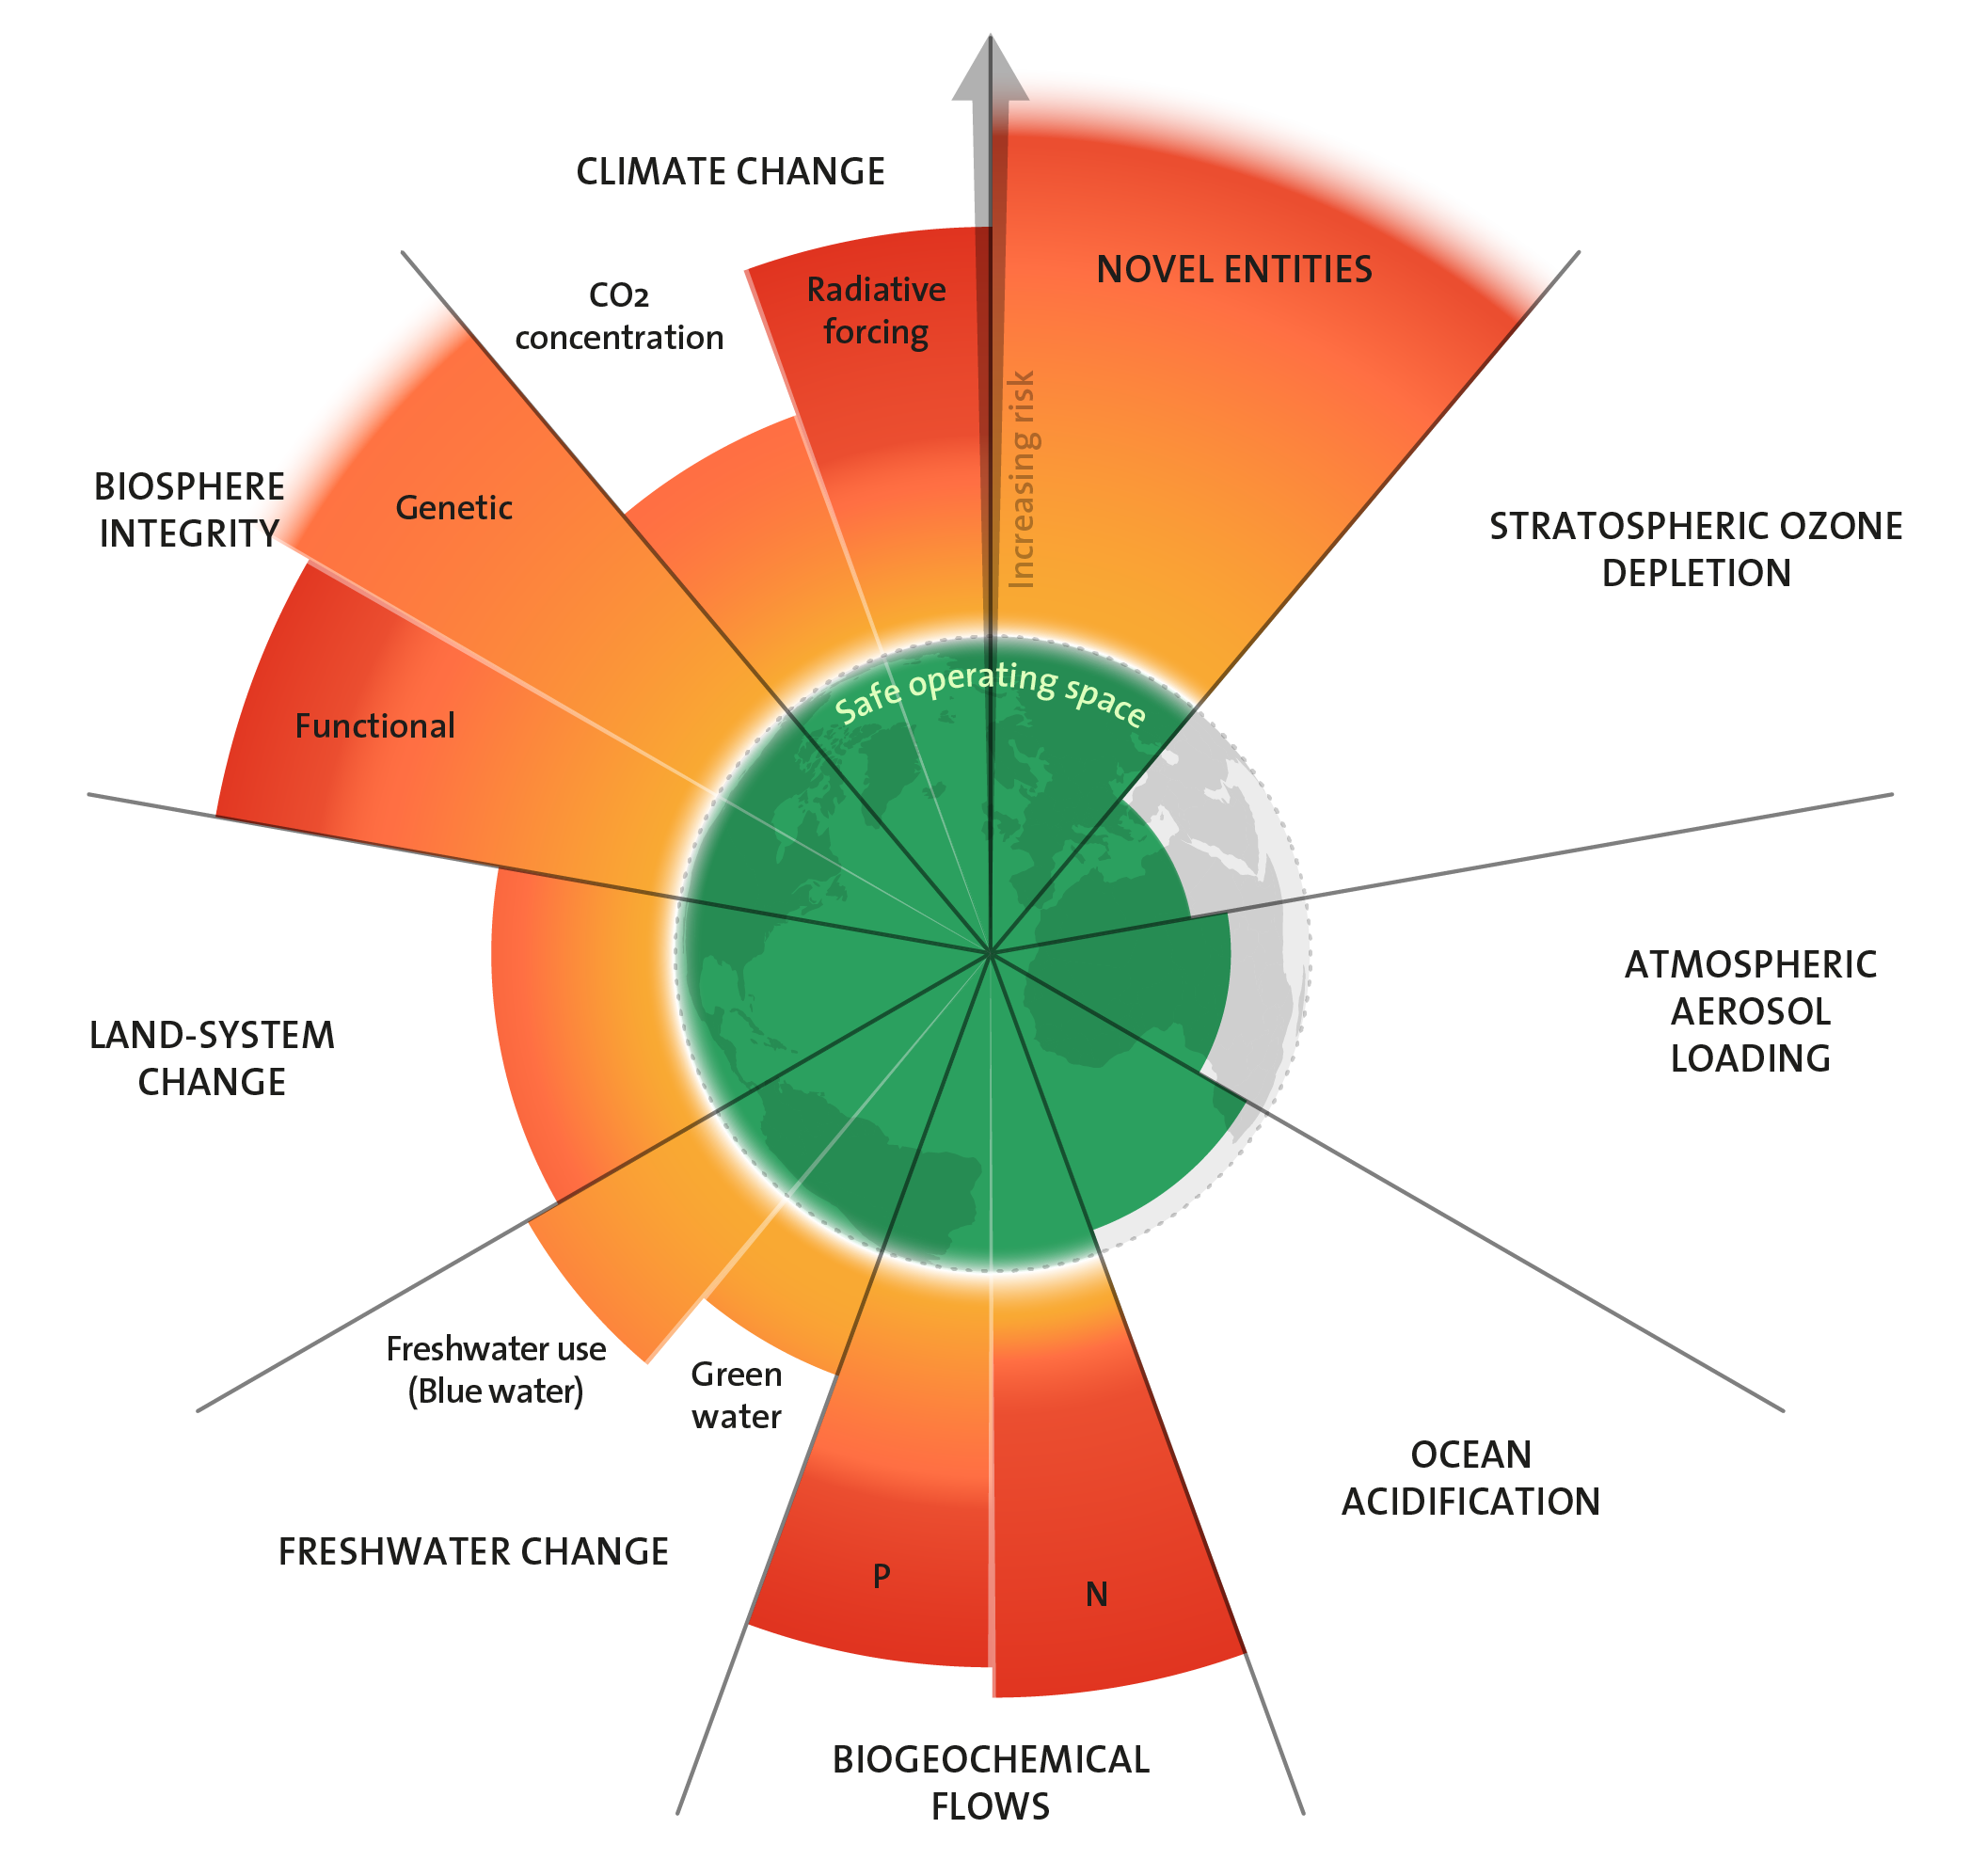
\includegraphics[width=1\textwidth,height=\textheight]{./images/sustainability/planetary-boundaries-2023.png}

}

\caption{Planetary Boundaries 2023 update. Azote for Stockholm
Resilience Centre, based on analysis in Richardson et al 2023}

\end{figure}%

In 1948, the International Union for Conservation of Nature (IUCN) was
founded, which in

LULUCF ``Land Use, Land-Use Change, and Forestry'' can both be a source
of greenhouse gas emissions - or a carbon sink (removing CO2 from the
atmosphere).

\subsubsection{\texorpdfstring{Earth System Law, Planetary Health, and
Social Cost of
CO\textsubscript{2}}{Earth System Law, Planetary Health, and Social Cost of CO2}}\label{earth-system-law-planetary-health-and-social-cost-of-co2}

\emph{Planetary Health}, \emph{Earth System Law, and} Social Cost of
Carbon are 3 approaches to address the complex interdependence of humans
with our physical environment.

Scientists in cross-disciplinary teams have been working on integrating
Earth systems and human society into cohesive frameworks.

Evolving Measurements from Planetary Boundaries to Planetary Health

\begin{itemize}
\item
  Planetary health (Planetary Health Alliance, 2024a, 2024b)
\item
  Wardani et al. (2023) \emph{``long-term human well-being is dependent
  on the well-being of the planet, including both biotic and abiotic
  systems. It recognizes interlinkages across environmental
  sustainability, public health, and socioeconomic development.''}
\end{itemize}

\emph{Earth System Law} is a framework for addressing interconnected
environmental challenges (Du Toit \& Kotzé, 2022).

\emph{Social Cost of Carbon} attempts to measures the compound impact of
CO\textsubscript{2e} emissions on society. Sustainability is filled with
complexities. CO\textsubscript{2e} emissions are complicated by
biodiversity loss, child labor, slavery, poverty, chemical pollution,
etc. - many issues become intertwined (TEDx Talks, 2020). One attempt to
measure these complexities, is the \emph{Social Cost of Carbon} (SCC)
which is defined as \emph{``additional damage caused by an extra unit of
emissions''} (Kornek et al., 2021; Zhen, Tian \& Ye, 2018). For example
the cost of damages caused by ``one extra ton of carbon dioxide
emissions'' (Stanford University, 2021). SCC variations exist between
countries (Tol, 2019) and regions (Wang, Ma \& Wang, 2022).

\begin{itemize}
\item
\item
  (Lin et al., 2022a) says, apart from CO\textsubscript{2}, reduction of
  other atmospheric pollutants, such as non-CO\textsubscript{2}
  greenhouse gases (GHGs) and short-lived climate pollutants (SLCPs) is
  required for climate stability.
\item
  (Wang \& Teng, 2022): Quantifying climate damage proposes scenarios of
  climate damage.
\end{itemize}

\subsection{Ecosystem Services: Quantifying Human Benefits from
Nature}\label{ecosystem-services-quantifying-human-benefits-from-nature}

\emph{Ecosystem services measure the benefits humans receive from the
biosphere.} Put most simply, \emph{ecosystem services} enable human life
on Earth. While it can be assumed much of the flora and fauna are
crucial for Earth's systems, science is still in the process of
understanding and quantifying its contributions. The history of the
valuation of nature's services goes back to the 18th century when David
Ricardo and Jean Baptiste Say discussed nature's \emph{work}, however
both considered it should be free (Gómez-Baggethun et al., 2010). In
1997 (Anon, 1997) proposed the idea of \emph{ecosystem services} and
(Costanza et al., 1997) attempted to assess the amount of ecosystem
services provided. (Le Provost et al., 2022)'s study shows
\emph{biodiversity} as one key factor to maintain delivery of ecosystem
services. (Noriega et al., 2018) attempts to quantify the ecosystem
services (ES) provided by insects.

The most complex computer models which attempt to capture ever more
interactions happening in the physical realm are called \emph{digital
twins.} The EU is developing a digital twin of Earth to help
sustainability prediction and planning, integrating Earth's various
systems such as climate, hydrology, ecology, etc, into a single model
Anon (2023f). We can use all the data being recorded to provide a
digital twin of the planet, nature, ecosystems and human actions to help
us change our behavior and optimize for planetary wellbeing.

\begin{itemize}
\tightlist
\item
  Jackson (1996) \emph{preventive environmental management}
\end{itemize}

\subsubsection{Biosphere}\label{biosphere}

Earth's biosphere is made up of 846 terrestrial ecoregions, which are
distributed across 14 major biomes and 8 biogeographical realms
(Dinerstein et al., 2017).

\subsubsection{Ecological Indicators}\label{ecological-indicators}

Sustainability can be measured using a variety of \emph{ecological
indicators}.

Ecological indicators for Earth \emph{- I would like to coin the word
``ecomarkers'' -} are like \emph{biomarkers} in human health.

Technological advances help scientist better understand nature. Cutting
edge research uses AI-based voice recognition for listening to nature,
assessing biodiversity based on species' sounds in the forest. Millions
of detections of different species with machine learning passive
acoustic AI models, can also assess species' response to climate change
(AI for Good, 2023; Guerrero et al., 2023).

\emph{Environmental DNA (eDNA)} helps scientists measure species
abundance without direct observation through detection of DNA on genetic
materials such as skin cells (Peter Andrey Smitharchive page, 2024).
Cellular DNA can be isolated from various sediment types (Ogram, Sayler
\& Barkay, 1987). Beyond scientific applications, eDNa is being used to
generate biodiversity credits by environmental asset rating companies
such as BeZero (Ojoatre \& Atkinson, 2023).

AI is being used to map icebergs and measure the change in size
(European Space Agency, 2023).

\subsubsection{Biodiversity}\label{biodiversity}

Why Protect Biodiversity?

(May, 2011) argues biodiversity loss is a concern for 3 points of views:

\begin{longtable}[]{@{}
  >{\raggedright\arraybackslash}p{(\columnwidth - 2\tabcolsep) * \real{0.3611}}
  >{\raggedright\arraybackslash}p{(\columnwidth - 2\tabcolsep) * \real{0.6389}}@{}}
\caption{From (May, 2011).}\tabularnewline
\toprule\noalign{}
\endfirsthead
\endhead
\bottomrule\noalign{}
\endlastfoot
View & \\
Narrowly Utilitarian & Biodiversity is a resource of genetic novelties
for the biotech industry. \\
Broadly Utilitarian & Humans depend upon biodiverse ecosystems. \\
Ethical & Humans have a responsibility to future generations to pass
down a rich natural world. \\
\end{longtable}

\begin{itemize}
\item
\item
  Meanwhile the destruction pressure on ecosystems is rapidly increasing
  (ADD CITATION A B C).
\item
  Chen et al. (2023) Ecosystem vulnerability \textbf{(need access)}
\item
  Zhang et al. (2023b) Integrating ecosystem services conservation into
  urban planning \textbf{(need access)}
\item
  Li et al. (2023) tourism is a large industrial sector which relies on
  ecosystem services. In Taiwan, (Lee, Jan \& Liu, 2021) developed a
  framework of indicators to assess sustainable tourism.
\end{itemize}

\textbf{Measuring Environmental Degradation}

(Almond, R.E.A. et al., 2022) reported, the number of species killed,
mass destruction of nature. ``69\% decline in the relative abundance of
monitored wildlife populations around the world between 1970 and 2018.
Latin America shows the greatest regional decline in average population
abundance (94\%), while freshwater species populations have seen the
greatest overall global decline (83\%).''

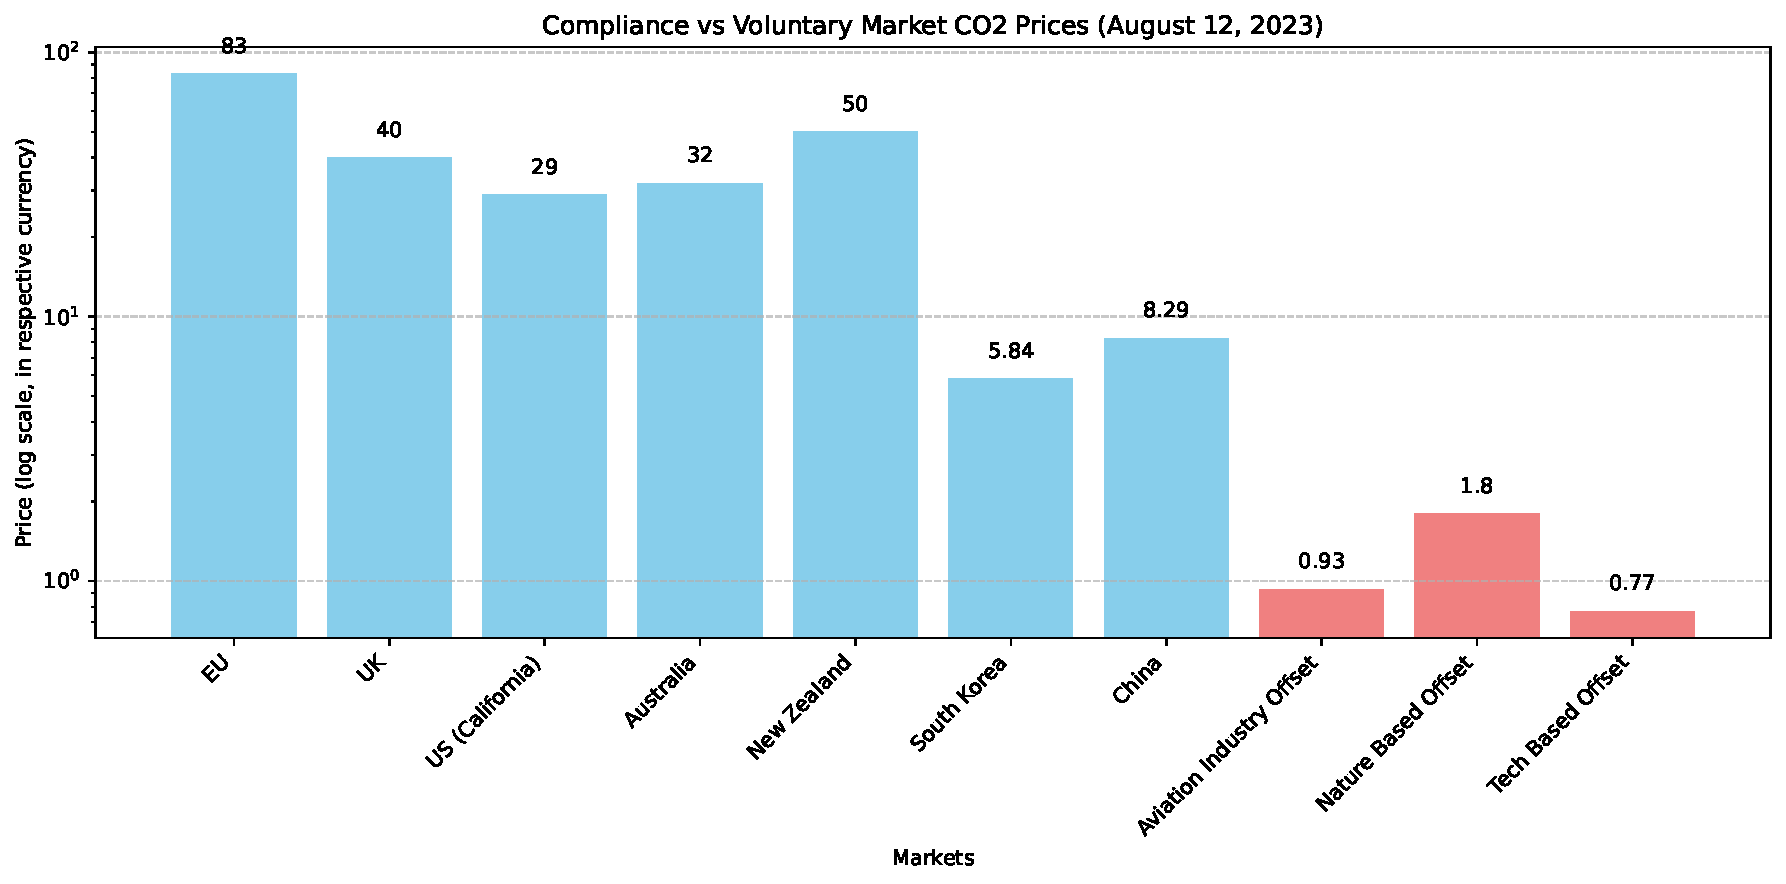
\includegraphics{_thesis_files/figure-pdf/cell-18-output-1.pdf}

Biodiversity loss is linked to overconsumption, weak legislation and
lack of oversight. (Crenna, Sinkko \& Sala, 2019) recounts European
Union consumers' negative impact on biodiversity in countries where it
imports food. WWF (2022) case study highlights how 4 biodiverse regions
Cerrado in Brazil, Chaco in Argentina, Sumatra in Indonesia, and the
Cuvette Centrale in Democratic Republic of Congo are experiencing rapid
destruction due to consumer demand in the European Union. While the
European Union (EU) has recently become a leader in sustainability
legislation, biodiversity protection measures among private companies is
very low Marco-Fondevila \& Álvarez-Etxeberría (2023).

Meanwhile, there is some progress in biodiversity conservation as
``{[}*b{]}iodiversity awareness is now at 72\% or higher in all
countries sampled, compared to only 29\% or higher across countries
sampled in 2009''* (UEBT, 2022)

\textbf{Convention on Biodiversity}

Similarly to climate protection, the UN has taken a leadership role in
biodiversity protection. Unit (2023): The history of the United Nations
Convention on Biodiversity goes back to 1988, when the working group was
founded. UNEP (Tue, 12/20/2022 - 07:44): The Convention on Biodiversity
2022 (COP15) adopted the first global biodiversity framework to
accompany climate goals.

Protecting biodiversity

\begin{longtable}[]{@{}
  >{\raggedright\arraybackslash}p{(\columnwidth - 2\tabcolsep) * \real{0.6111}}
  >{\raggedright\arraybackslash}p{(\columnwidth - 2\tabcolsep) * \real{0.3889}}@{}}
\caption{Biodiversity loss data from (Bradshaw et al.,
2021).}\tabularnewline
\toprule\noalign{}
\endfirsthead
\endhead
\bottomrule\noalign{}
\endlastfoot
What Happened? & How Much? \\
Vertebrate species population average decline & 68\% over the last 50
years \\
Land surface altered by humans & 70\% of Earth \\
Vertebrate species extinct & 700 in 500 years \\
Plant species extinct & 600 in 500 years \\
Species under threat of extinction & 1 million \\
\end{longtable}

\subsubsection{Oceans}\label{oceans}

Blue carbon.

\textbf{Marine Heatwaves}

\begin{itemize}
\tightlist
\item
  Gelles \& Andreoni (2023) describe how marine heatwaves threaten
  global biodiversity. Ocean warming leads to coral bleaching of the
  Great Barrier Reef in Queensland, east coast of Australia (Pfeiffer,
  2024).
\item
  Espinosa \& Bazairi (2023) marine ecosystem services \textbf{(need
  access, ncku doesn't sub)}
\item
  Howard et al. (2017) argues Oceans play crucial role in carbon
  capture.
\end{itemize}

\subsubsection{Forest}\label{forest}

Forests are a crucial part of Earth's carbon cycle and the main natural
CO\textsubscript{2} capture system; due to deforestation, Europe rapidly
losing its forest carbon sink (Frédéric Simon, 2022). Around 27\% of
Earth's land area is still covered by forests yet \emph{deforestation}
is widespread all around the world; highest rates of deforestation
happened in the tropical rainforests of South America and Africa, mainly
caused by agricultural cropland expansion (50\% of all deforestation)
and grazing land for farm animals to produce meat (38,5\%), totaling
close to 90\% of global deforestation (Anon, 2022f). The global forest
cover change is visible on Google's Earth Engine (Hansen et al., 2013).

Around the world, there are many initiatives to increase forest cover,
for example the \emph{1 billion tree project} (Greenfield \&
@pgreenfielduk, 2021; Anon, 2020; Bastin et al., 2019). However, it's
important to not planting trees (\emph{afforestation)} is not the full
solution, as \emph{afforestation} is different from
\emph{reforestation}, which takes into account biodiversity. Also, while
using remote-sensing and machine-learning to assess reforestation
potential (see Klosterman et al., 2022), it doesn't take into account
local political realities.

\begin{itemize}
\tightlist
\item
  Burning of biomass undermines carbon capture.
\item
  Bousfield et al. (2022) reports there's evidence paying landowners for
  the ecosystem services their forests provide may reduce deforestation.
\item
  nature-based solutions.
\end{itemize}

\subsubsection{Pollution}\label{pollution}

Health and sustainability are inextricably linked. ``Human health is
central to all sustainability efforts.'', \emph{``All of these (food,
housing, power, and health care), and the~stress~that the lack of them
generate, play a huge role in our health''} (Sarah Ludwig Rausch \& Neha
Pathak, 2021).

\textbf{Air Pollution}

Clean air is a proposed as a \emph{human right} (Baroness Jones of
Moulsecoomb \& Caroline Lucas, 2023) yet air pollution is widespread
around the planet, with 99\% of Earth's human population being affected
by bad air quality that does not meet WHO air quality guidelines,
leading to health problems linked to 6.7 million \emph{premature deaths}
every year (World Health Organization, 2022).

Air pollution is linked to cancer incidence. In Taiwan, South Korea, and
England, groundbreaking research by (Lim et al., 2022) analyzed over
400000 individuals establishes exposure to 2.5μm PM (PM2.5) air
pollution as a \emph{cause for lung cancer.} In (Hannah Devlin, 2022),
professor Tony Mok, of the Chinese University of Hong Kong: \emph{``We
have known about the link between pollution and lung cancer for a long
time, and we now have a possible explanation for it. As consumption of
fossil fuels goes hand in hand with pollution and carbon emissions, we
have a strong mandate for tackling these issues -- for both
environmental and health reasons.''}

The main way to combat air pollution is through policy interventions.
(MARIA LUÍS FERNANDES, 2023) the EU has legislation in progress to curb
industrial emissions. If legislation is in place, causing bad air
quality can become bad for business. In China, (Gu et al., 2023) links
air pollution to credit interest rates for business loans; companies
with low environmental awareness and a history of environmental
penalties pay 12 percent higher interest rates. In France, (Bouscasse et
al., 2022) finds strong health and economic benefits across the board
from air pollution reduction.

\textbf{Water Pollution}

Globally, 4.4 billion people only have access to water that's not safe
for drinking (Soliman, 2024).

\begin{itemize}
\item
  Bioswales help catch storm debris and reduce water pollution.
\item
  Clean water and water pollution
\item
  Koch (2022) (\textbf{Need access! NYC times)}
\item
  Paris cleans Seine river for Paris Olympics
\end{itemize}

\textbf{Soil Pollution}

\begin{itemize}
\tightlist
\item
  \emph{``Wild and ruderal plants as bioindicators of global urban
  pollution by air, water and soil in Riyadh and Abha, Saudi Arabia''}
  (Picó et al., 2023) uses wild and ruderal plants to detect pollution
  by air, water and soil.
\item
  Bioindicators of anthropogenic pollution, pharmaceuticals, pesticides,
  and other industrial chemicals.
\item
  Both Abha and Riyadh showed notable levels of pollutants while Riyadh
  with more industry showed higher levels.
\end{itemize}

\subsubsection{Ready for Disaster}\label{ready-for-disaster}

The Word Economic Forums Global Risks Report 2024 paints a bleak picture
of the future with expectations of increased turbulence across the board
based on a survey of over 1400 topic experts (World Economic Forum,
n.d.).

\subsubsection{Weather}\label{weather}

Global warming increases the risk of disasters and extreme weather
events.

(Anon, 2023i) The US Global Change Research Program presented a
comprehensive report to the US Congress, which links disaster-risk
directly to global warming; for examples increased wildfires damage
property, endanger life and reduces \emph{air quality,} which in effect
increases health challenges. As extreme temperatures are increasingly
commonplace, with observed changes in heatwaves, there's increased risk
of wildfires (Volkova, Roxburgh \& Weston, 2021; Perkins-Kirkpatrick \&
Green, 2023), while flood risk mapping might lower property prices in at
risk areas (Sherren, 2024). Summers of 2022 and 2023 were the hottest on
record so far, with extreme heat waves recorded in places around the
world (Venturelli et al., 2023; Serrano-Notivoli et al., 2023; Douglas,
2023; National Oceanic and Atmospheric Administration (NOAA), U.S.
Department of Commerce, 2023; NOAA National Centers for Environmental
Information, 2023; Falconer, 2023).

The part of Earth where the \emph{human climate niche} is becoming
smaller (McKibben, 2023). As temperatures rise, certain cities may
become uninhabitable for humans (CBC Radio, 2021). The summer of 2023
saw extensive wildfires in Spain, Canada, and elsewhere; rapidly moving
fires destroyed the whole city of Lāhainā in Hawaii {[}ADD CITATION{]}.
In California, (Jerrett, Jina \& Marlier, 2022) says,
\emph{``{[}w{]}ildfires are the second most important source of
emissions in 2020''} and \emph{``negate reductions in greenhouse gas
emissions from other sectors.''} Some parts of South America have seen
summer heat \emph{in the winter}, with heatwaves with temperatures as
high as 38 degrees (Livingston, 2023).

In Taiwan disaster risk and hazard mapping is well-developed, with early
warning systems, and comprehensive response preparedness - and painful
experiences - instrumental to saving lives (Tsai et al., 2021).
Intensifying storms forming near coastlines, can be expected with
\emph{``{[}c{]}hanges to tropical cyclone trajectories in Southeast Asia
under a warming climate''} (Garner et al., 2024). The situation on the
Pacific and Atlantic oceans is not dissimilar, with
\emph{``{[}o{]}bserved increases in North Atlantic tropical cyclone peak
intensification rates''} (Garner, 2023).

In the Phillipines, with increasing extreme weather events,
\emph{``businesses are more likely to emerge in areas where
infrastructure is resilient to climate hazards''} (Cheng \& Han, 2022).

Climate-related disasters can spur action as extreme weather becomes
visible to everyone. After large floods in South Korea in July 2023 with
many victims, president Joon promised to begin taking global warming
seriously and steer the country towards climate action (Web, 2023; AFP,
2023; Al Jazeera, 2023). South Korea has a partnership with the European
Union (European Commission, 2023a).

\begin{itemize}
\tightlist
\item
  Chernobyl and Fukushima
\item
  the Great Pacific Garbage Patch
\item
  Disputes in Eerola (2022).
\end{itemize}

\subsection{Financialization of Nature vs Nature is Sacred: Scaling Up
Sustainable
Action:}\label{financialization-of-nature-vs-nature-is-sacred-scaling-up-sustainable-action}

There are 2 main approaches to protecting nature:

\begin{longtable}[]{@{}
  >{\raggedright\arraybackslash}p{(\columnwidth - 2\tabcolsep) * \real{0.3611}}
  >{\raggedright\arraybackslash}p{(\columnwidth - 2\tabcolsep) * \real{0.6389}}@{}}
\toprule\noalign{}
\endhead
\bottomrule\noalign{}
\endlastfoot
\textbf{Economics of Nature Commodification} & \textbf{Economics of the
Sacred} \\
Measure and assign monetary value to nature. & Nature is Sacred - such
as are religious holy places - and can't be touched (Eisenstein, 2011,
2018) \\
\end{longtable}

\begin{itemize}
\tightlist
\item
  (Leverhulme Centre for Nature Recovery, 2023) asks should we put a
  price on nature?
\item
  Is it time to leave utilitarian environmentalism behind? Muradian \&
  Gómez-Baggethun (2021)
\end{itemize}

\begin{longtable}[]{@{}l@{}}
\caption{From (Leverhulme Centre for Nature Recovery,
2023).}\tabularnewline
\toprule\noalign{}
\endfirsthead
\endhead
\bottomrule\noalign{}
\endlastfoot
9 Steps \\
Identify ecosystem functions \\
Quantify ecosystem functions \\
Identify ecosystem services \\
Quantify ecosystem services \\
Quantify financial value of ecosystem services \\
Assign property rights \\
Create ecosystem service markets \\
Commodify nature \\
\end{longtable}

\subsubsection{Individual Action}\label{individual-action}

Sometimes individual environmental (climate) action \emph{does matter}
and can come at great personal cost, even loss of life. EJAtlas tracks
environmental justice cases around the world, where human stakes are
very high Scheidel et al. (2020).

However, for most of us individual climate action is \emph{ineffective}.
The effect of individual climate action such as \emph{choosing a more
sustainable product} is so limited to be next to meaningless. For
individual consumer choices to make a difference, they need to be
\emph{aggregated} into a movement, collective action with scale,
influence, and visibility.

There is no single solution to the environmental crisis. Given the
enormity of environmental degradation, many different approaches are
needed. This chapter documents some of the ongoing work which a
sustainability companion could assist college students get involved
with.

\subsubsection{Restoration}\label{restoration}

Regenerative Action

\begin{itemize}
\tightlist
\item
  (Han \& Chen, 2022) identifies nature-based solutions ``land
  re-naturalization (such as afforestation and wetland restoration)''
\end{itemize}

\begin{longtable}[]{@{}l@{}}
\caption{From Han \& Chen (2022)}\tabularnewline
\toprule\noalign{}
Non-Exhaustive list of \\
\midrule\noalign{}
\endfirsthead
\toprule\noalign{}
Non-Exhaustive list of \\
\midrule\noalign{}
\endhead
\bottomrule\noalign{}
\endlastfoot
Afforestation \\
Wetland restoration \\
 \\
\end{longtable}

Ecology, Agroforestry \& Permaculture

Some argue sustainability is not enough and we should work on
\emph{regeneration} of natural habitats.

The UN announced 2021-2030 the Decade on Ecosystem Restoration (Fischer
et al., 2021).

\begin{itemize}
\tightlist
\item
  Agroecology Baltic Sea Action Group (2023)
\end{itemize}

Agroforestry plays an active role in achieving Sustainable Development
Goals (SDGs) (Ruba \& Talucder, 2023);

\begin{itemize}
\tightlist
\item
  Food forests for regenerative food systems.
\item
  Svalbard Seed Vault
\item
  Irwin et al. (2023)
\item
  Yadav et al. (2023)
\item
  Low, Dalhaus \& Meuwissen (2023)
\item
  Ollinaho \& Kröger (2023) ``bioeconomy is not inherently sustainable
  and may pose considerable risks to biodiversity.''
\item
  De Queiroz-Stein \& Siegel (2023)
\item
  Gamage et al. (2023) ``Organic food and drink sales in 2019 totaled
  more than 106 billion euros worldwide.''
\end{itemize}

Geopolitical situations can affect technology adoption; after Russia's
war in Ukraine, Europe needed to quickly reduce consuming cheap Russan
fossil fuel energy (in the form of gas) (Bonasia, 2024). In 2024, for
first time in Europe, renewables in the form of wind and solar energy
surged past production of fossil fuels (Graham \& Fulghum, 2024; Beer,
2024)

EU energy mix in 2024

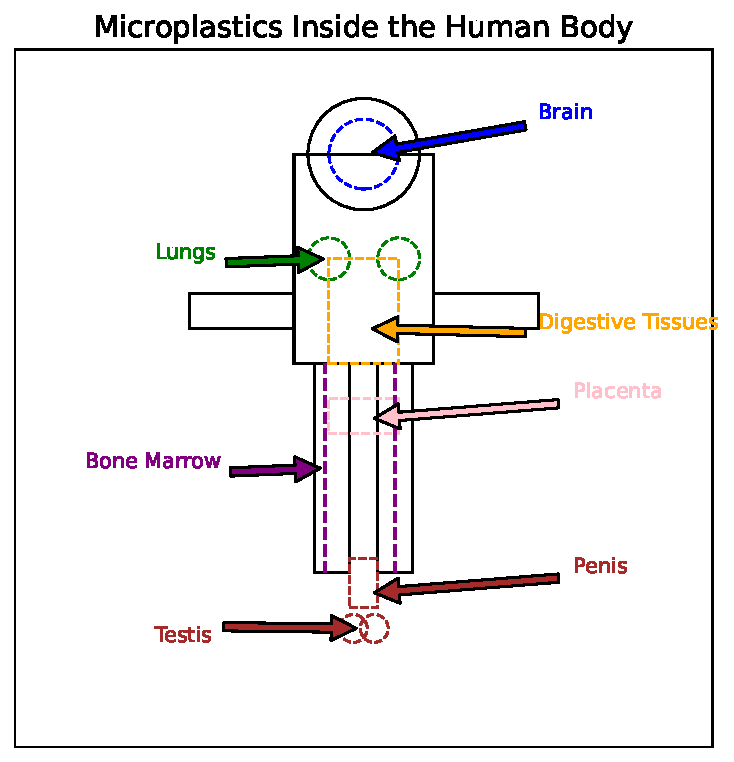
\includegraphics{_thesis_files/figure-pdf/cell-19-output-1.pdf}

Wind and solar energy overtook fossil energy.

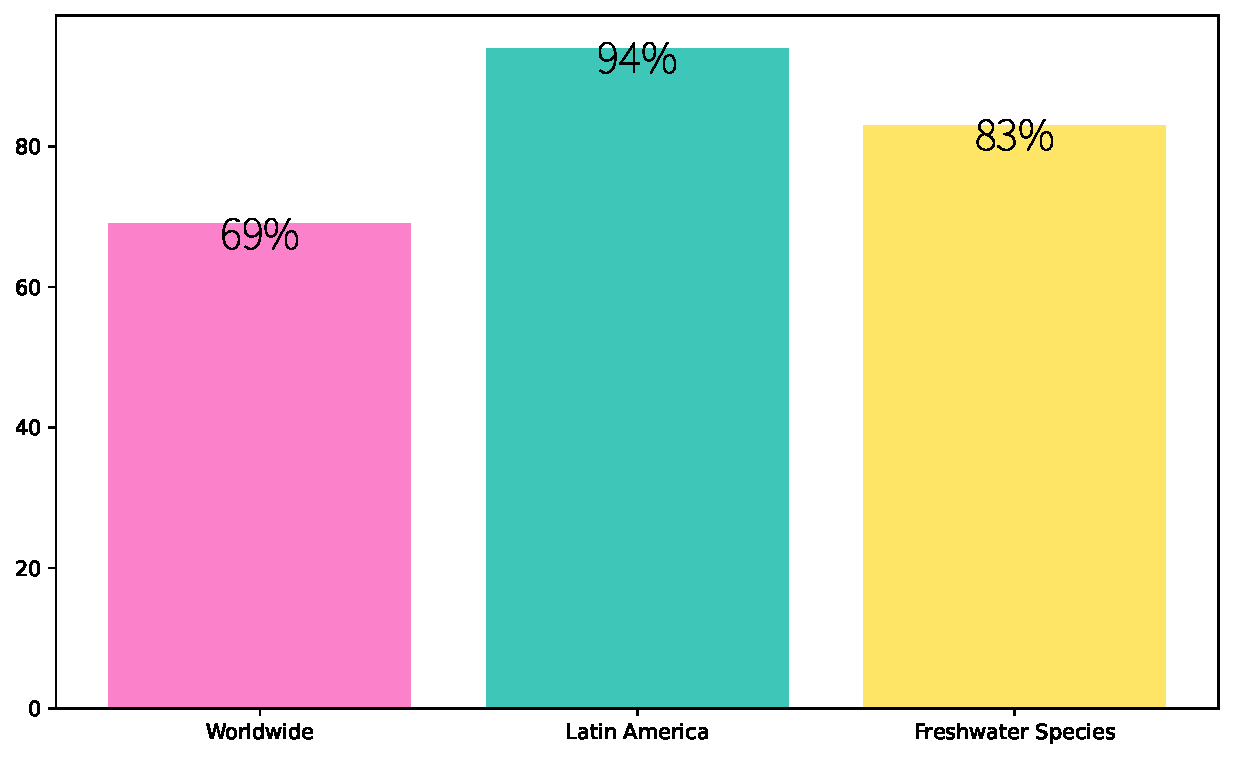
\includegraphics{_thesis_files/figure-pdf/cell-20-output-1.pdf}

Meanwhile reduction in coal-power was also possible. Coal is a large CO2
emitter.

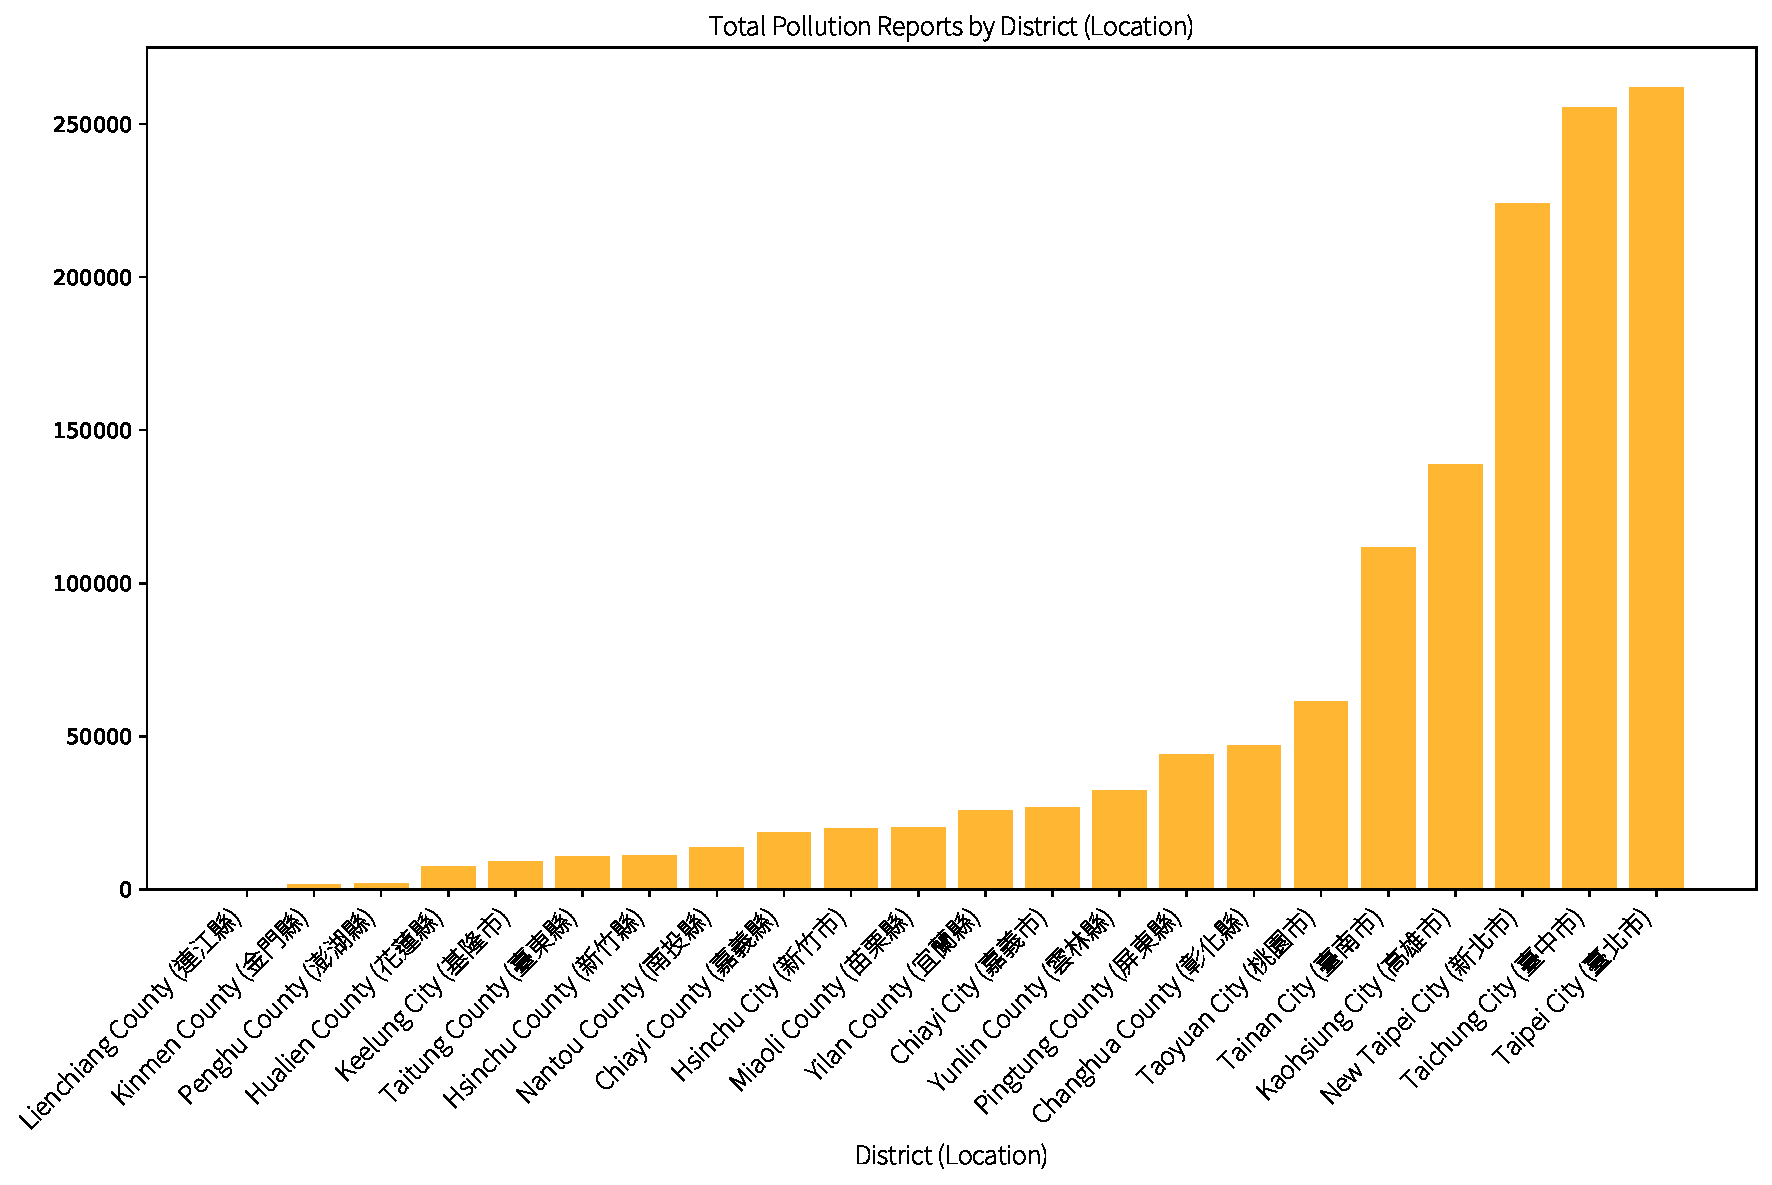
\includegraphics{_thesis_files/figure-pdf/cell-21-output-1.pdf}

``Climatech'', Renewable Energy and Transforming Energy Production

Large technology conglomerates and newly founded startups working in
climate solutions space (often referred to as \emph{climatech} by the
media) have proposed a range of approaches to CO\textsubscript{2}
reduction in Earth's atmosphere. These technologies include several
types of \emph{carbon capture}, directly from the air (direct air
capture or DAC), from the source of pollution, such as using
high--performance filters on factory chimneys, as well as nature-based
solutions such as large scale tree planting using drones.

Each technology has their own pros and cons. (Vitillo et al., 2022)
illustrates how direct air capture of CO\textsubscript{2} is difficult
because of low concentration and CO\textsubscript{2} capture at the
source of the emissions is more feasible.

\begin{itemize}
\item
  (Gaure \& Golombek, 2022) simulate a CO\textsubscript{2} free
  electricity generation system in the European Union where ``98\% of
  total electricity production is generated by wind power and solar; the
  remainder is covered by a backup technology.''. The authors stipulate
  it's possible to power the EU without producing CO\textsubscript{2}
  emissions.
\item
  \textbf{Important: ``creating sustainability trust in companies in
  realtime''}
\end{itemize}

\subsection{Complexity: Towards Probabilistic Risk-Based
Assessment}\label{complexity-towards-probabilistic-risk-based-assessment}

Sustainability is a complex web of interconnections.

\begin{itemize}
\item
  thread of commodification of nature. category mistake. impossible to
  bring back already destroyed biodiversity which took millennia to
  develop. humans create hugely complex systems instead of simply
  conserving nature.
\item
  The concept of how a public resource is over-used until breaking down
  as each user only bears a fraction of the cost - know as \emph{tragedy
  of the commons} -was described by the ecologist Garrett Hardin in 1968
  (Hardin, 1968; Meisinger, 2022; Lopez, Pastén \& Gutiérrez Cubillos,
  2022; Murase \& Baek, 2018).
\end{itemize}

\subsection{Design Implications}\label{design-implications-1}

\begin{longtable}[]{@{}
  >{\raggedright\arraybackslash}p{(\columnwidth - 2\tabcolsep) * \real{0.3611}}
  >{\raggedright\arraybackslash}p{(\columnwidth - 2\tabcolsep) * \real{0.6389}}@{}}
\caption{Implications}\tabularnewline
\toprule\noalign{}
\endfirsthead
\endhead
\bottomrule\noalign{}
\endlastfoot
Category & Implication \\
Transparency & In unison, the reviewed technologies and practices move
us closer to enabling \emph{realtime ESG}: up-do-date transparent
information about how our product are produced. \\
Speed & Realtime ESG is a building block to enable consumers and
investors make more accurate, real-world purchase decisions. \\
Actionability & Simplify action \\
Pollution & \emph{People live in the polluted areas are so used to it.
What app to wake them up? ``You live in a highly polluted area. Here's
the TOP 10 companies causing pollution. Here's what you can do.''} \\
Health Tracking & Blood testing and biomarkers allow people to track
their health. I'm introducing the concept of `eco-markers' to follow the
sustainability of human activities. \\
Circular Economy & AI can help us make sense of the vast amounts of
sustainability data generated daily. \\
EPR & ERP and CDP data should be part of Green Filter. \\
Eco-Design & How to find eco-designed products? \\
CE and EPC & Encouraging Sustainable Design \\
Politics Matter & \\
& Call for GOP contributors' transparency \\
& ``triple turn'' \\
& Lack of transparency \\
& Sustainability is part of product quality. If a product is hurting the
environment, it's a low quality product. \\
\end{longtable}

\subsection{Feature Ideas}\label{feature-ideas-1}

\begin{longtable}[]{@{}ll@{}}
\toprule\noalign{}
\endhead
\bottomrule\noalign{}
\endlastfoot
\textbf{Category} & \textbf{Idas} \\
& \\
& \\
\end{longtable}

\newpage

\section{Design}\label{design}

\begin{figure}[H]

{\centering 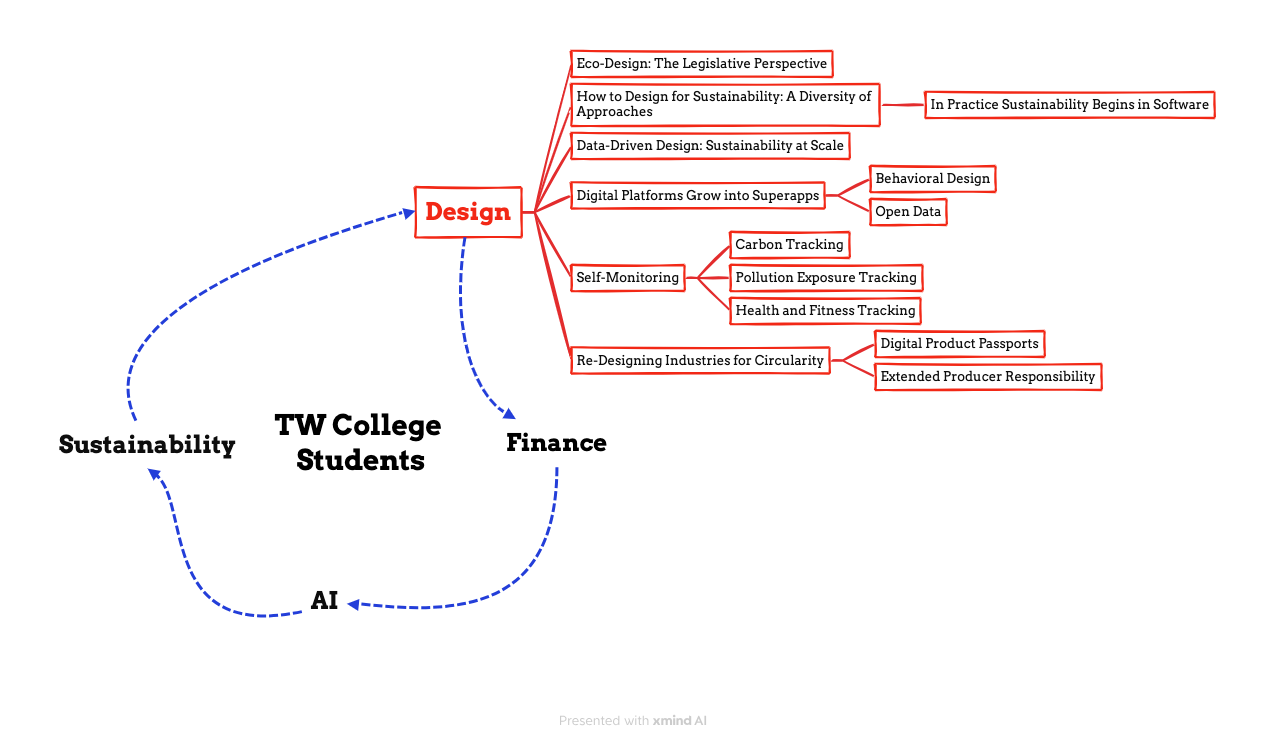
\includegraphics{./images/design/abstract-design.png}

}

\caption{Visual abstract for the design chapter}

\end{figure}%

\subsection{Eco-Design: The Legislative
Perspective}\label{eco-design-the-legislative-perspective}

In Europe, \emph{eco-design} has strong political support as part of the
European Union's (EU) ``Green Deal'' legislative strategy, aiming to
transform European economies into sustainability leaders. The Ecodesign
for Sustainable Products Regulation (ESPR) entered into force in the EU
on July 18, 2024 (European Commission, 2024) following the (European
Parliament, 2022) proposal whereby the European Commission established a
general framework for \emph{eco-design: ``requirements for sustainable
products, repealing rules {[}referring to the previous Eco-Design
Directive (2009/125/EC){]} currently in force which concentrate on
energy-related products only,''} setting up a level playing-field for
the organizations operating on the EU single market. Virginijus
Sinkevičius, the EU Commissioner for the Environment, Oceans and
Fisheries, is quoted describing eco-design as design that
\emph{``respects the boundaries of our planet''} (European Commission,
2022c).

Eco-Design is a Key EU Sustainable Policy Design Tool. A large part of
the proposal by (Commission et al., 2014) is \emph{eco-design}, as a
large part of product lifecycle environmental impact is defined in the
design process.

\begin{longtable}[]{@{}lll@{}}
\toprule\noalign{}
\endhead
\bottomrule\noalign{}
\endlastfoot
Quality & & \\
Durable & Reparable & Easy to recycle \\
Reusable & Easy to maintain & Energy efficient \\
Upgradable & Easy to refurbish & Resource efficient \\
\end{longtable}

Sustainable Products and EUDR (European Union Deforestation Regulation)
work hand-in-hand as part of EU's legislative efforts to promote
sustainability.

EUDR applies to all products placed on the market from 30 December 2024
and 30 June 2025 for small businesses.

ESPR, EUDR

ESRS, CSRD (Corporate Sustainability Reporting Directive) replaces NFRD
(Non-Financial Reporting Directive)

EU ``Green Deal'' legislative is comprehensive.

ESRS reporting standard to meet CSRD requirements.

\begin{itemize}
\tightlist
\item
  Anon (2021a)
\item
  Switch2Green (2023)
\end{itemize}

It's up to legislators to provide sustainable products on our
marketplace\ldots{} but until we do, use the green filter.

\begin{itemize}
\tightlist
\item
  One of the EU goals is reducing consumption
\item
  Tacking our consumption habits
\item
  Europe is the hotbed of sustainability
\item
  Iman Ghosh (2020)
\item
  Lamoureux (2018) Florida sustainable companies
\item
  MICHAEL HOULIHAN \& BONNIE HARVEY (2018) customers prefer sustainable
  companies
\item
  In the US, the \emph{Inflation Reduction Act} provides funding to
  development of decarbonizing technologies and includes plans to combat
  air pollution, reduce green house gases and address environmental
  injustices (Rajagopalan \& Landrigan, 2023).
\end{itemize}

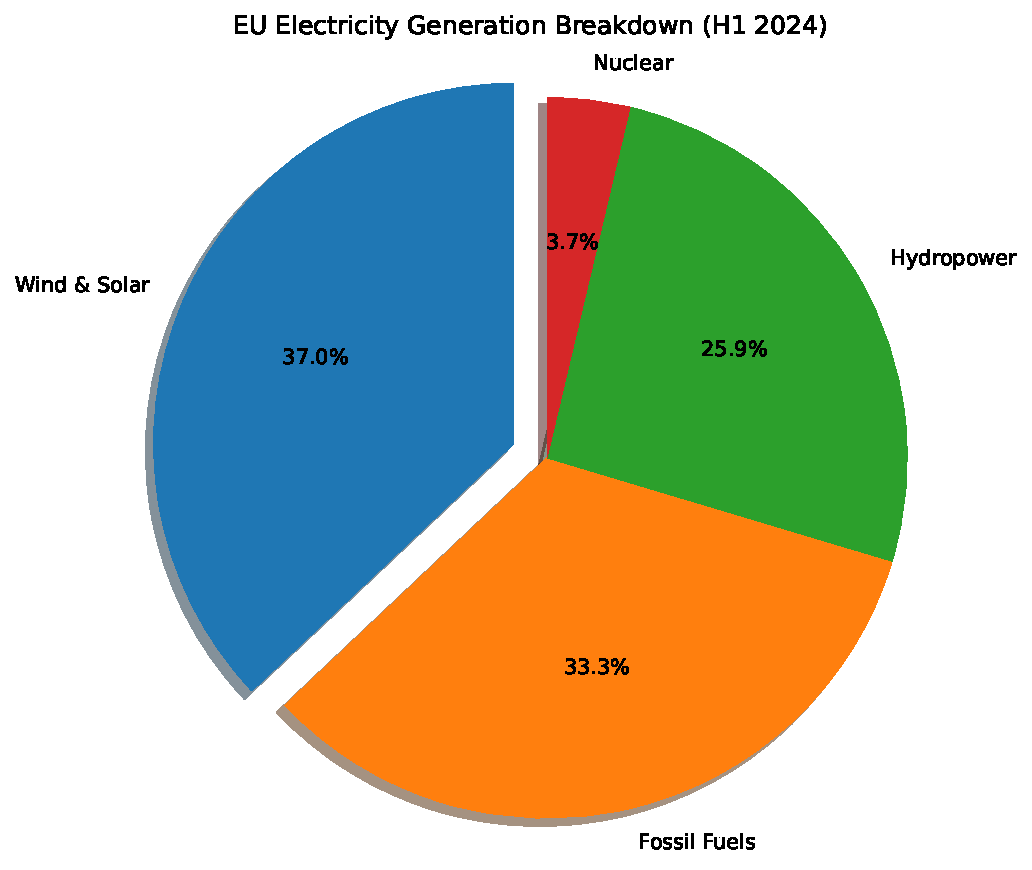
\includegraphics{_thesis_files/figure-pdf/cell-23-output-1.pdf}

Many other jurisdictions also have laws that aim to reduce the
environmental impact of products throughout their life cycles. For
instance Australia has a Product Stewardship (PS) scheme, which also
includes an investment fund targeted at increasing the recycling rates
of specific products (Australian Government, 2024). Australia, Japan,
and Taiwan all have Sustainable Procurement schemes prioritizing greener
products in public purchases {[}ADD CITATION{]}. While Taiwan doesn't
yet have a specific eco-design law, there are various pieces of
legislation promoting circular economy {[}ADD CITATION{]}. Already in
1988 Taiwan implemented an Extended Producer Responsibility (EPR)
scheme, followed by a recycling system (initially focused on electronic
items) in 1998 (Chong et al., 2009). Eco-design initiatives in Taiwan
started at least as early as 1994, when Taiwanese companies and
universities noticed international sustainability trends and began to
implement their own sustainable design initiatives (Jahau Lewis Chen et
al., 2005).

The key to comparing Product Stewardship, Extended Producer
Responsibility (EPR), and Eco-Design is the scope, as illustrated in the
chart below. While Product Stewardship (PS) and Extended Producer
Responsibility (EPR) deal mostly with the end of the product lifecycle
(they are \emph{reactive}), including their disposal and recycling (EPR
going a step further than PS by shifting the responsibility to the
producer), Eco-Design moves sustainability up the design chain (being
\emph{pro-active}), setting standards for making better products - in
essence, attempting to \emph{design-out} the waste.

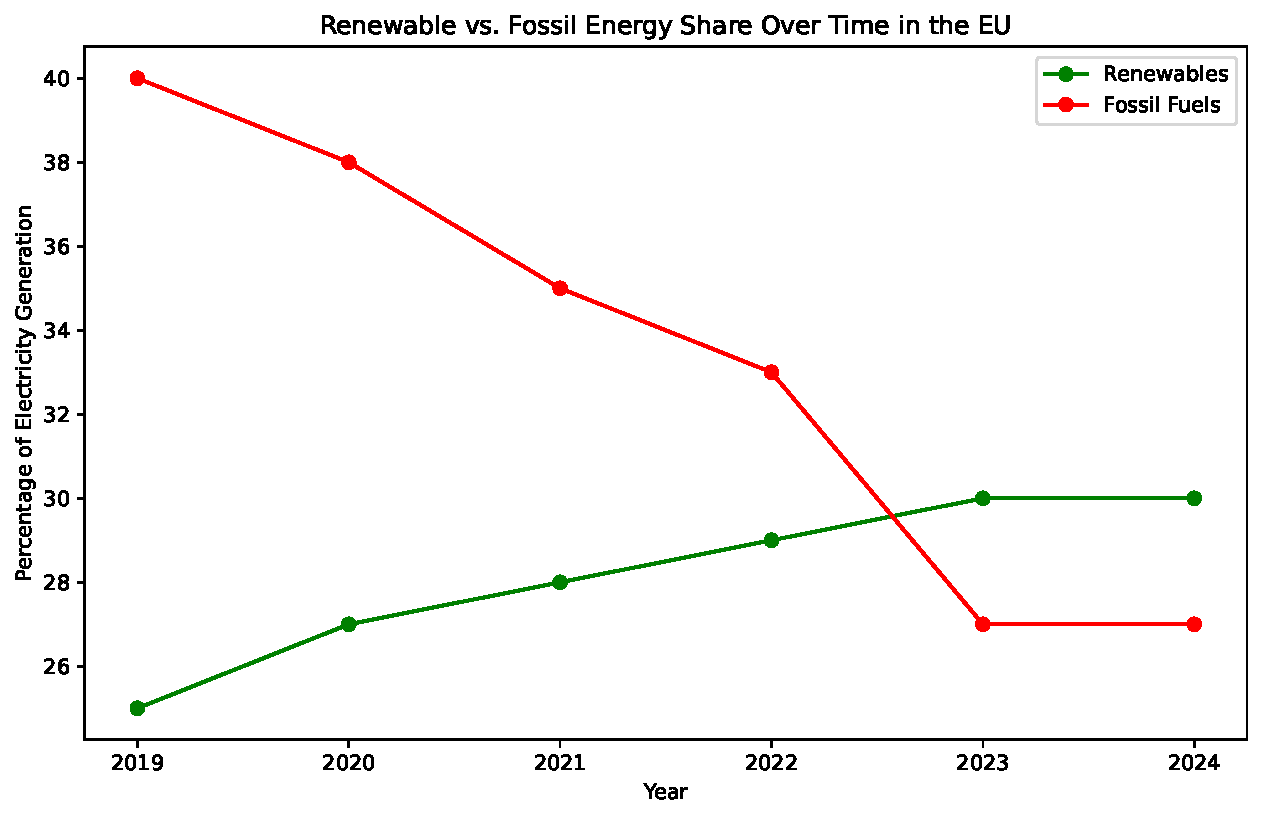
\includegraphics{_thesis_files/figure-pdf/cell-24-output-1.pdf}

\subsection{Political Action}\label{political-action}

I was torn whether to put politics under Sustainability or Design, and
decided for the latter - as sustainability is most descriptive, using
science to measure and present the real situation, while Design - like
politics - is prescriptive: making decisions about how do we live.

Design \emph{is} political.

\begin{itemize}
\tightlist
\item
  Pater (2021)
\item
  10 countries use almost 100\% renewable energy
\end{itemize}

There's ample evidence from several countries suggesting moving to
renewal energy brings environmental benefits:

\begin{itemize}
\item
  Amin et al. (2022) suggests ``removing fossil fuel subsidies and
  intra-sectoral electricity price distortions coupled with carbon taxes
  provides the highest benefits'' for both the economy and the
  environment in Bangladesh.
\item
  Luo et al. (2022) suggests using reinforcement learning to reduce
  energy use in cooling systems.
\item
  Montreal protocol eradicates CfCs and the ozone holes became whole
  again.
\end{itemize}

\textbf{\emph{Mitigating}} \textbf{Climate Change}

The monumental task of removing several gigatons of CO\textsubscript{2}
from the atmosphere requires massive policy shifts and collaboration
across countries and industries (Mackler, Fishman \& Broberg, 2021).

Warming global climate has concrete effects on daily life. Warmer
climate helps viruses and fungi spread (Press, 2023). (Williams \&
Joshi, 2013) higher CO\textsubscript{2} concentrations in the air can
cause more turbulence for flights.

\textbf{\emph{Adapting}} \textbf{to Climate Change}

Many companies are developing technologies for mitigation.

Politics matters in sustainability. In Brazil, deforestation fell 60\%
in 1 year, based on remote satellite reconnaissance, after the election
of a more pro-environment leadership (Watts, 2023).

\begin{itemize}
\tightlist
\item
  Eesti Vabariigi Valitsus (2022) Estonian Green Deal Action Plan (Eesti
  Rohepöörde Tegevusplaan).
\end{itemize}

In the European Union (EU), a wide range of legislative proposals,
targets, organizations, and goals already exists across diverse
countries. Upcoming laws aim to harmonize approaches to sustainability
and raise standards for all members states, in turn influencing
producers who wish to sell in the EU common market.

\begin{itemize}
\tightlist
\item
  (Anon, n.d.x) report: The EU has a \emph{taxonomy of environmentally
  sustainable economic activities} published by the Technical Expert
  Group (TEG) on sustainable finance.
\end{itemize}

\textbf{Taxes}

\begin{itemize}
\tightlist
\item
  There have been proposal of a ``meat tax''.
\end{itemize}

\textbf{SDGs}

\begin{itemize}
\item
  SDGs need to discussed in their totality Popkova et al. (2022).
\item
  German Institute of Development and Sustainability (IDOS) connects
  SDGs to NDCs. Dzebo, Iacobuţă \& Beaussart (2023)
\item
  International Energy Agency (IEAs), Decarbonisation Enablers IEA
  (2023b)
\end{itemize}

Sustainbility Policy context is Shifting Around the World

\begin{itemize}
\item
  ``In the context of the EU Plastics Strategy, the European Commission
  has launched a pledge to increase the use of recycled content to 10
  million tons by 2025. To address this, Circularise Plastics Group
  launched an ``Open Standard for Sustainability and Transparency''
  based on blockchain technology \& Zero-knowledge Proofs'' Circularise
  (2020b)
\item
  ``data-exchange protocol with privacy at its heart'' Circularise
  (2020a)
\item
  EU AI Law Lomas (2024)
\end{itemize}

\textbf{Kunming-Montreal Global Biodiversity Framework}

\begin{itemize}
\item
  The proposal for a Nature Restoration Law by the European Commission
  requiring member countries to restore 20\% of EU's degraded ecosystems
  by 2030 and full restoration by 2050 has not yet passed Anon (2023ac)
  and is facing a backlash David Pinto (2023).
\item
  Manzardo et al. (2021) \textbf{(need access!)}
\item
  Iñarra et al. (2022) \textbf{(need access!)}
\item
  Munaro, Tavares \& Bragança (2022) \textbf{(need access!)}
\item
  Bassani et al. (2022) \textbf{(need access!)}
\item
  Van Doorsselaer (2022) \textbf{(need access!)}
\end{itemize}

Calculating what's sustainable is hugely complex because decisions may
have unforeseen ramifications. For example (Nuez, Ruiz-García \& Osorio,
2022) shows how electric vehicles may increase CO\textsubscript{2}
emissions in some areas, such as Canary Islands, where electricity
production is polluting.

\begin{itemize}
\item
  Rossi, Cappelletti \& Germani (2022) shows how introducing
  sustainability early in the design process and providing scenarios
  where sustainability is a metric, it's possible to achieve more
  eco-friendly designs.
\item
  Arranz, Sena \& Kwong (2022) developing circular economy is really
  complex
\item
  Cheba et al. (2022)
\item
  Ruiz-Pastor et al. (2022)
\item
  Miyoshi et al. (2022) takes the example of ink toner bottles and shows
  in a case study how standardized compatibility between older and newer
  systems can save resources and results in sustainability savings.
\item
  Finding green products and supporting companies making them
\item
  Supporting legislative changes
\item
  Track you consumption, saving, investing. Shift balance towards saving
  and investing.
\item
  Nastaraan Vadoodi (2022)
\item
  European Commission (2022b) Ecodesign for sustainable products
\end{itemize}

\textbf{Europe From 2023 to 2030}

\begin{itemize}
\tightlist
\item
  EU releases strategic foresight reports since 2020 (European
  Commission, 2023b).
\end{itemize}

\begin{figure}[H]

{\centering 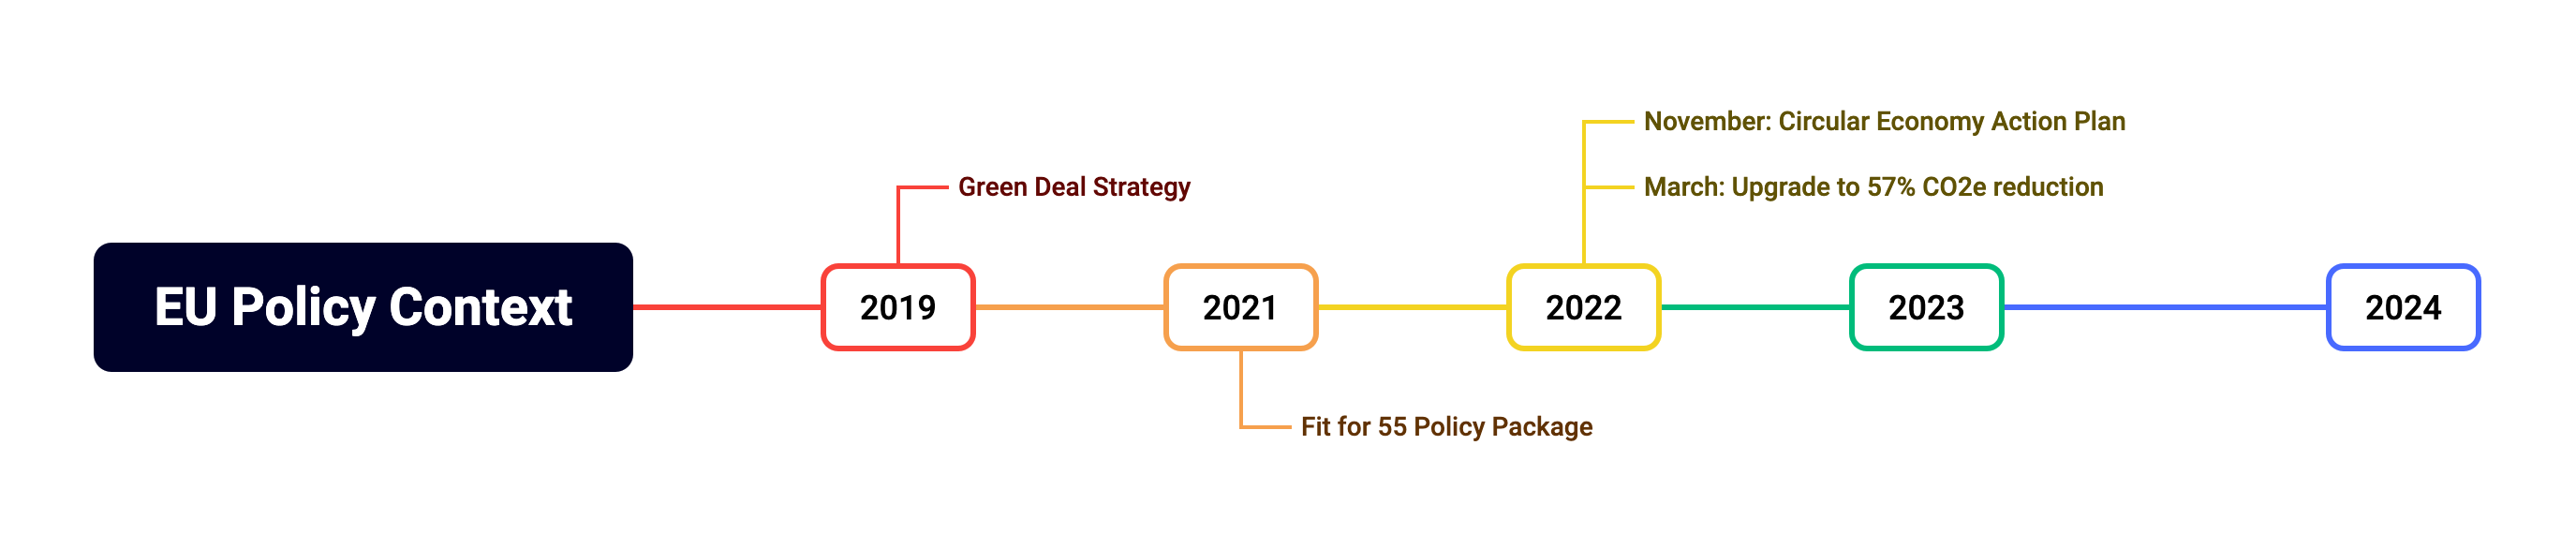
\includegraphics[width=1\textwidth,height=\textheight]{./images/sustainability/eu-policy-context.png}

}

\caption{EU Policy Context Timeline}

\end{figure}%

We have an opportunity to re-imagine how every product can be an
eco-product and how they circulate in our circular economy.

Timeline of the Policy Context:

\begin{itemize}
\item
  In 2019 by the von der Leyen commission adopted the European Union
  (EU) Green Deal strategy.
\item
  In 2021 the Commision proposed a goal of reducing CO2e emissions by
  55\% by 2030 under the \emph{Fit for 55} policy package consisting of
  a wide range of economic measures.
\item
  In November 2022, the proposal was adopted by the EU Council and EU
  Parliament with an updated goal of 57\% of CO2e reductions compared to
  1990. This proposal is set to become a binding law for all EU member
  countries (European Commission (2019c); European Commission (2019a);
  Anon (2022d); European Council (2022)).
\item
  In March 2022, the EU Circular Economy Action Plan was adopted,
  looking to make sustainable products \emph{the norm} in EU and
  \emph{empowering consumers} as described in European Commission
  (2022a). Each product covered by the policy is required to have a
  \textbf{\emph{Digital Product Passport}} which enables improved
  processing within the supply chain and includes detailed information
  to empower consumers to understand the environmental footprint of
  their purchases. It's safe to say the large majority of products
  available today do not meet these criteria.
\end{itemize}

\textbf{Quality of Life}

Wellbeing Economy Governments is an Example of Country-level
Collaboration

\begin{itemize}
\tightlist
\item
  Finland, Iceland, New Zealand, Scotland, Wales, Canada (Fioramonti et
  al., 2022).
\item
  Kaklauskas et al. (2023)
\item
  Anon (2023al) Integrated science of wellbeing
\item
  Fabris \& Luburić (2022)
\end{itemize}

\subsection{How to Design for Sustainability: A Diversity of
Approaches}\label{how-to-design-for-sustainability-a-diversity-of-approaches}

\emph{Designing for Sustainability} \emph{(DfS)} has many names, with
subtle differences of emphasis and nuance. While the ESPR legislation
chose \emph{Eco-Design} as the overarching title, researchers and
practitioners discuss and use \emph{Circular Design},
\emph{Cradle-to-Cradle Design}, \emph{Green Design}, \emph{Regenerative
Design}, \emph{Climate-Responsive Design}, \emph{Life-Centered Design},
and many others.

In most cases, designing for sustainability makes use of \emph{systems
thinking}, underlining the importance of looking at the entire lifecycle
of a product or service. Sustainable design encompasses all human
activities, making this pursuit an over-arching challenge across all
industries and all human activities with the complex interdependencies
contained within. (Ceschin \& Gaziulusoy, 2016) gives a comprehensive
overview of the main themes of sustainable design and the main
contributions and limitations in the well--researched \emph{``Evolution
of design for sustainability: From product design to design for system
innovations and transitions''}.

R. Buckminster Fuller ``Operating Manual for Spaceship Earth'', Victor
Papanek ``Design for the Real World'', Jonathan Chapman ``Emotionally
Durable Design'', Carlo Vezzoli ``Product-Service System Design for
Sustainability'', Ezio Manzini ``Design, When Everybody Designs''.

\emph{Service Design}, Ceschin \& Gaziulusoy (2016) shows how design for
sustainability has expanded from a product focus to systems-thinking
focus placing the product inside a societal context of use. For example
Anon (n.d.i), recycled clothing maker FREITAG offers
sustainability-focused services such as cargo bikes so you can transport
your purchases and a network for \emph{shopping without payment} =
swapping your items with other members, as well as repairs of their
products. Loaning terminology from \emph{service design}, the user
journey within an app needs to consider each touchpoint on the way to a
state of success.

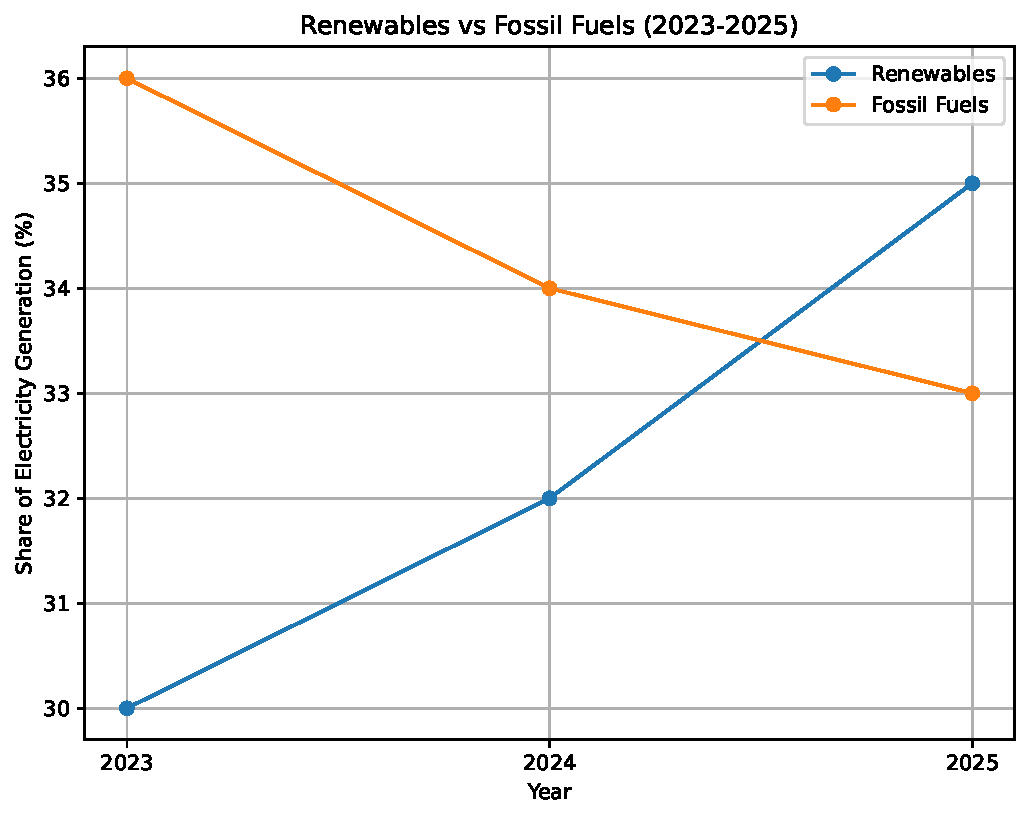
\includegraphics{_thesis_files/figure-pdf/cell-25-output-1.pdf}

As this research is \emph{practice-oriented} (i.e., my goal here is to
find design approaches that could influence my prototype), I will focus
on some fields of design which I hope relevant, fruitful, or contextual
to my project.

I will start with \emph{Human-Centered Design}, the grandfather of
design with attitude. There's even an ISO standard for human-centered
design, with the designated code ISO9241-210, revised as ISO
9241-210:2019 titled \emph{``Ergonomics of human-system interaction''}
and up for revision soon (ISO standards are reviewed every 5 years).
Some of the key takeaways include ``Understanding and specifying the
context of use'', ``Involving users throughout design and development'',
``Specifying user requirements'', ``Evaluating designs'',
``Multi-disciplinary Collaboration'', ``Iterative process'' and
``Continual Improvement'', and finally - usability is not enough, the
design should provide a user experience (UX) for human ``emotional
responses and satisfaction'' (ISO, 2019).

While \emph{Human-Centered Design} focuses exactly on what it says -
humans - \emph{Life-Centered Design} recognizes human impact on our
surrounding environment as well - making sure we include non-human
animals among our stakeholders. This is where we are getting on the
\emph{territory} of sustainability. While \emph{Human-Centered Design}
is ever popular, the effect humans are having on biodiversity is rarely
considered when designing. \emph{``{[}T{]}he design phase of a physical
product accounts for 80\% of its environmental impact''}
notes(Borthwick, Tomitsch \& Gaughwin, 2022) in their framework for
life-centered design.

If we're including \emph{other} lifeforms among our stakeholders, what
can we learn from them? \emph{Biomimicry} is about being inspired by
nature while \emph{Biodesign} focuses on design involving biology in the
design itself. Janine Benyus, who coined the word \emph{Biomimicry}
(Benyus, 2009) looks at very practical cases of innovation where
engineers and biologist meet and (Dicks, 2023) provides a much more
philosophical account of following the example of nature. Focusing on
the financial sector, (Thomas \& Mantri, 2022)'s philosophical account
advocates for an ``inside-out'' design pattern, much like natural
systems, starting from the smallest structures to guarantee resilience
and survival, instead of trying to control their external environment.

In a similar vein, \emph{Material Ecology} is the wording preferred by
the architect Neri Oxman based at the MIT Media Lab working with
biomaterials as a proponent of \emph{Nature-Centric Design} that adheres
to the principles of ecological sustainability with both an ecologically
conscious mindset and practical toolset (Hencz, 2022). Language and our
mental concepts shape our reality, which makes language-creation an
important tool for sustainability. Neri Oxman's expressions in her
(World Economic Forum, 2016) interview introduce some new vocabulary:
\emph{``ecology-indifferent''}, \emph{``naturing''}, \emph{``mother
naturing''}, \emph{``design is a practice of letting go of all that is
unnecessary''}, \emph{``nature should be our single client''}, which
reminds me how self-invented language gives un child-like freedom to
imagine new worlds.

\emph{Speculative Design} can help us imagine \emph{non-anthropocentric}
(Hupkes \& Hedman, 2022; Edwards \& Pettersen, 2023)as well as
\emph{dystopian} futures (Pinto et al., 2021). First introduced by
(Dunne \& Raby, 2013) in their seminal book, the field aims to question
the intersection of \emph{user experience design} and \emph{speculative
fiction}. (Barendregt \& Vaage, 2021) explores the potential of
speculative design to stimulate public engagement; thought experiments
can spur public debate on an issue chosen by the designer. Phil
Balagtas, founder of The Design Futures Initiative at McKinsey,
discusses the value of building future scenarios at his talk at Google.
His favorite example, the Apple Knowledge Navigator, first appeared in
an Apple vision video in 1987 and took two decades to materialize in the
real world. It was inspired by a similar device first shown in a 1970s
episode of Star Trek as a \emph{magic device} (a term from participatory
design), which then inspired subsequent consumer product development. It
took another two decades, until the launch of the iPhone in 2007 - a
total of 40 years.

\emph{Participatory Design} and \emph{Speculative Design} can be
complementary as in the work of (Neuhoff, Simeone \& Laursen, 2023),
used together to focus on engaging users deep in the design process to
truly understand their needs, contexts and interactions on a
non-superficial level. For both speculative and participatory design,
the cost and makes it into a niche activity. Generative AI holds the
promise to allow designers to dream up and prototype quicker. In order
to build a future, it's relevant to imagine and critique a future. By
being quickly generate prototypes, once can test out ideas with the
future users involving more of the community and stakeholders. To be
able to build something, one first needs to imagine it; imagination is
crucial for change.

\emph{Speculative Design} helps us envision future scenarios

Massachusetts Institute of Technology (MIT) is a source of many
fantastic innovations, and another.

\emph{Regenerative Design} suggests \emph{de}materializing (digitizing)
economies is not enough to be sustainable (by reduction of physical
impact). Design should look beyond reducing harm and find avenues to
\emph{regenerate} damaged or even completely destroyed natural systems
-- ecosystems, biodiversity, land, forests, lakes, rivers - natural
habitats.

Sufficiency

Moving from products and (digital) experiences towards the built
environment and architecture, \emph{Climate-Responsive Design} embeds a
building within the environmental constraints of a place and looks for
opportunities use the land, wind, sun, local materials, and local
vernacular history and culture when considering a design. Architect
Susanne Brorson suggests sustainability should be considered in the
earlier phases of design instead of trying to fix problems later
discussing \emph{climate-responsive design principles} (EVM
maaarhitektuuri keskus, 2019). The sentiment is echoed by (Lee \&
Doevendans, 2011) who edited a volume on sustainable approaches of
world-renowned architects: \emph{``The principles of sustainable design
are rooted in the building's relationship to the site and its
environmental conditions such as topography, vegetation, and climate.''}

Architecture of the Well-Tempered Environment (Banham, 1999)

\emph{Designing for Trust}, Weinschenk (2011) says \emph{``People expect
most online interactions to follow the same social rules as
person-to-person interactions. It's a shortcut that your brain uses to
quickly evaluate trustworthiness.''}

\emph{Cradle-to-Cradle Design}, focusing on recyclability of products.
Anon (2021r) and 活動通 (n.d.) Cradle to Cradle Nordic circular design
in Taiwan

\emph{Durability} is an important dimension for sustainability. High
quality durable products are more sustainable as they last longer and
less likely to be thrown away. Forming an emotional bond with the
product makes it feel more valuable (Zonneveld \& Biggemann, 2014).
(Chapman, 2009) argues in his seminal paper (and later in his book) for
\emph{``Emotionally Durable Design''}, the simple idea that we hold to
things we value and thus they are sustainable. We don't throw away a
necklace gifted to us by mom, indeed this object might be passed down
for centuries. (Rose, 2015) has a similar idea, where \emph{``Enchanted
Objects''} become so interlinked with us, we're unlikely to throw them
away. This has implications for sustainability as the object is less
likely to be thrown away.

As the above shows, there are many partially overlapping design words
created by different people for diverse purposes. Design vocabulary may
be created for distinguishing a particular type of design from another -
or to market oneself as the creator of the word. There are designers who
define / brand themselves by their design method. Design Studies, a
field that studies \emph{design} as a subject.

Here I will use the lens of \emph{sustainability} - another complex term
- to look at how design can contribute to eco-friendly products. I
advocate looking at design methods as a toolbox, where I can pick the
tool suitable for the problem set in front of me. Here I look at a small
number of design practices I find relevant to designing a sustainability
app for college students.

than traditional design methods. While AI allows us to look at a larger
number of design scenarios thank previously feasible, there are many
approaches looking for ways to design for sustainability. Designing for
Sustainability is fundamentally a hopeful act imbibed with the dream a
healthier world is possible.

\subsubsection{Future Scenarios: Avoiding the Worst
Cases}\label{future-scenarios-avoiding-the-worst-cases}

In sustainability there are rarely good choices. Rather it's a question
of avoiding the worst choices.

\emph{Scenario-building} is a key tool for sustainability. Because
sustainability is so complex, sustainable design makes use of scenarios.

\emph{Life Cycle Assessment} and \emph{Environmental Impact Analysis}
are needed to provide eco-design scenarios (de Otazu et al., 2022).

user experience, iteration (Google Design, 2019)

\subsubsection{In Practice Sustainability Begins in
Software}\label{in-practice-sustainability-begins-in-software}

Designing user interfaces for sustainable interactions means
incorporating data and toolsets to enable designers to make decisions
which reduce emissions of their design. Companies like AutoDesk are
putting CO\textsubscript{2} calculations inside their design software,
helping designers reduce material usage, energy consumption,
CO\textsubscript{2} emissions, while increasing recyclability(Mike
Haley, 2022). Software is key to building more sustainable products,
already for decades (Gupta et al., 2023). AI-assisted design enables
design for sustainability because the design process is where
sustainability begins. AI has the potential to provide the parameters
for sustainability. (Singh \& Sarkar, 2023) proposes an AI tool for
deciding the suitable life cycle design parameters.

Design encompasses most everything in our daily lives. Humans live in
artificial environments where \emph{most} \emph{things} are designed by
humans. The \emph{experiences} we take part in are increasingly created
based on some type of data.

\begin{itemize}
\tightlist
\item
  Involving young HCI designers in AI-oriented workshops can show the
  future of UI/UX ? (Battistoni et al., 2023)
\end{itemize}

\emph{Data is the interface} between idle resources and retail demand,
which makes \emph{exchange of value} possible.

\begin{itemize}
\tightlist
\item
  Different Gets Ignored Luke Wroblewski (2024)
\end{itemize}

\emph{Digital Sustainability}, information pertaining to emissions would
flow through the economy not unlike the carbon cycle itself.

\begin{itemize}
\tightlist
\item
  Pan \& Nishant (2023) important
\end{itemize}

Interaction Design for Climate Change: how can we change common UIs so
they take into account sustainability?

\begin{itemize}
\tightlist
\item
  UIA World Congress of Architects (2023) ``Design for climate
  adaptation''
\item
  Andrew Chaisson (2019)
\item
  Dzigajev (2019)
\item
  Mankoff et al. (2007)
\item
  Borthwick, Tomitsch \& Gaughwin (2022)
\item
  Lose (2023b) is worried about applying UX skills for Climate Change
\end{itemize}

AI-Assisted Design

\textbf{Tool vs Assistant? (Tools are mostly non-anthropomorphic?).}
Tools do not call attention to themselves. They don't necessarily rely
on human-like representations that call attention to themselves but
rather are available in-context to help streamline specific tasks.

\begin{itemize}
\tightlist
\item
  September 16, 2020 (2020) ``What is AI-assisted Design?''
\item
  Clipdrop (n.d.) AI Design Assistants
\item
  Architechtures (2020) Architecture with the help of AI
\item
  Zakariya (2022) Canva image generator
\item
  Kore.ai (2023) Kore.ai developing custom AI-chatbots for business
  usage.
\item
  Anon (n.d.j) storytelling by AI
\end{itemize}

\subsection{Data-Driven Design: Sustainable Personalization at
Scale}\label{data-driven-design-sustainable-personalization-at-scale}

Data-Driven Design Enables Sustainability. Sustainability touches every
facet of human existence and is thus an enormous undertaking. Making
progress on sustainability is only possible if there's a large-scale
coordinated effort by humans around the planet. For this to happen,
appropriate technological tools are required.

Data-driven design has limitations.

Coputer

One mode

\begin{itemize}
\tightlist
\item
  Konings (2020)
\item
  ``Digital sustainability principles''
\item
  Eminent journal Design Studies, 1st design journal
\item
  Part of digital product design are \textbf{design systems} to keep
  consistency across the experience. Create a design system to best to
  showcase my analytic skills:

  \begin{itemize}
  \tightlist
  \item
    Design System:
    https://zeroheight.com/8bf57183c/p/82fe98-introduction
  \item
    Anon (n.d.e)
  \item
    Suarez et al. (n.d.)
  \item
    Anon (n.d.as)
  \item
    Anon (n.d.f)
  \end{itemize}
\item
  Kolko \& Connors (2010) and IxDF (n.d.) believe interaction design is
  still an emerging (and changing) field and there are many definitions.
  I prefer the simplest version: interaction design is about creating a
  conversation between the product and the user.
\item
  AI gives designers new tools. In AI development, design is called
  alignment. What is the role of an AI Designer? Linden (2021)
\item
  Anon (n.d.bc)
\item
  Anon (n.d.ao)
\item
  Parundekar (2021)
\item
  Richard Yang (2021) and Justin Baker (2018) say some of the tools used
  by interaction designers include
\item
  AI for design: Figma (2023)
\end{itemize}

The concept of \emph{Social Objects}: People need something to gather
around and discuss. Sharing.Lab (2015): I'm interested in the concept of
a ``social object''.

\emph{Red Route Analysis} is an user experience optimization idea
inspired by the public transport system of London (Oviyam™, 2019; Anon,
2021j; Xuan, 2022).

\begin{itemize}
\tightlist
\item
  Product marketers focus on the \emph{stickiness} of the product,
  meaning low attrition, meaning people keep coming back.
\item
  What percent of all design is ``sustainable design'' ? Promoting
  sustainable design.
\item
  Josh Luber (2021) Trading cards are cool again
\item
  Jesse Einhorn (2020)
\item
  Connie Loizos (2021)
\item
  Natasha Mascarenhas (2021)
\item
  JEFF JOHN ROBERTS (April 23, 2020 at 2:00 PM GMT+3)
\end{itemize}

\emph{Narrative Design,} Humans respond well to
\textbf{\emph{storytelling}}, making \textbf{\emph{character design}}
and \textbf{\emph{narrative design}} relevant to interaction design.
Large language models (LLMs) such as ChatGPT are able to assume the
personality of any character that exists inside of its training data,
creating opportunities for automated narrative design.

\begin{itemize}
\item
  The rising availability of AI assistants may displace Google search
  with a more conversational user experience. Google itself is working
  on tools that could cannibalize their search product. The examples
  include Google Assistant, Google Gemini (previously known as Bard) and
  large investments into LLMs.
\item
  Alethea AI (2021): discusses writing AI Characters, creating a
  personality.
\item
  Writing as training data? large language models. GTP3.
\item
  Stories start with a character.
\end{itemize}

\subsubsection{Designing for College
Students}\label{designing-for-college-students}

\begin{itemize}
\tightlist
\item
  plap
\end{itemize}

\subsubsection{Personalization}\label{personalization}

\begin{itemize}
\tightlist
\item
  Personal User Experience. social apps require personalization, trust
  and k-factors (sharing and inviting your friends). (Baron, 2023; Kim,
  2023).
\end{itemize}

\subsubsection{Growth Design}\label{growth-design}

\begin{itemize}
\item
  For digital products (apps) the main application of interaction design
  is for \emph{growth} in usage, how to get more people (user journey
  and conversion funnels) to use the product i.e user acquisition,
  retention, engagement, and monetization and keep using it (retention
  and engagement), often optimizing onboarding, features, and
  personalization (Steger, 2019; Kende, 2023).
\item
  Hypothesis and validation for iterating on features.
\item
  Total addressable market (TAM), serviceable addressable market (SAM),
  target audience (TA)
\end{itemize}

\subsection{Digital Platforms Grow into
Superapps}\label{digital-platforms-grow-into-superapps}

Superapps are the latter stage of the Digital Platform Economy.

Platform economy companies popularized and expanded Data-Driven Design
in the service of growth marketing (also known colloquially as growth
hacking). Capturing User Data was part of this strategy which enabled
improving the products. Digital Product Design is increasingly
data-driven. Digital platforms operate a \emph{design as a process} in a
continuous feedback loop, where \emph{measurements}, \emph{experiments,}
predictive analytics and personalization form a data-drive design
culture. As we humans go about our daily business, governments and
companies track our activities using various technologies, which
produces massive amounts of user interaction data. Platform economy
companies are the capture and use large amounts of data from users. Data
is useful for designing better products. Designing for high retention
(users keep coming back). Network Effects, the more people use a
platform, the more valuable it becomes. Platforms that continuously add
features (provided consumer legislation allows it) may eventually evolve
into superapps, which are useful for providing services for a wide
category of human needs. Bundling many services under one super-brand.
Superapps are possible thanks to Nudge, Economies of Scale, Network
Effects, Behaviour Design. Large Digital Platforms have a very small
number of workers relative to the number of users they serve. This
creates the necessity for using automation for both understanding user
needs and providing the service itself. Creating a good product that's
useful for the large majority of users depends on \emph{Data-Driven
Design.}

Design is as much about how it works as it's about the interface.

Digital product design can be seen as a specific discipline under the
umbrella of Experience Design. In Michael Abrash (2017) Meta Oculus
augmented reality incubation general manager Laura Fryer: \emph{``People
buy experiences, not technology.''}

Young people expect a product. Intelligent Interfaces use interaction
design to provide relevant and personalized information in the right
context and at the right time.

There are many approaches to design - from playful to practical to
critical and to data-driven. Nonetheless, many types of design share a
common goal designing for a good \emph{user experience}. Simplifying.

\emph{Personalization}: the largest businesses today (measured in number
of users) design the whole user experience.

\emph{Scale,} Popular consumer platforms strive to design solutions that
feel personalized at every touchpoint on the user journey (to use the
language of service design) at the scale of hundreds of billions of
users.

Superapps are honeypots of data that is used for many types of behavior
modeling. (Suarez et al., 2021) suggests using alternative data from
super-apps to estimate user income levels, including 4 types of data:
Personal Information, Consumption Patterns, Payment Information, and
Financial services. (Roa et al., 2021) finds super-app alternative data
is especially useful for credit-scoring young, low-wealth individuals.
The massive amounts of data generated by these companies are used by
smart cities to re-design their physical environments.

Twitter (now X) is becoming a financial app.

Inspiration from WeChat.

How can the mobile devices which the majority of us are carrying with us
every day, help us make decisions about the businesses we engage with?
In terms of user experience, can personalized AI advisors empower our
financial actions from shopping to saving and investing?

\begin{longtable}[]{@{}
  >{\raggedright\arraybackslash}p{(\columnwidth - 4\tabcolsep) * \real{0.1289}}
  >{\raggedright\arraybackslash}p{(\columnwidth - 4\tabcolsep) * \real{0.3828}}
  >{\raggedright\arraybackslash}p{(\columnwidth - 4\tabcolsep) * \real{0.4844}}@{}}
\toprule\noalign{}
\begin{minipage}[b]{\linewidth}\raggedright
Enablers of Platform Economics
\end{minipage} & \begin{minipage}[b]{\linewidth}\raggedright
Pros
\end{minipage} & \begin{minipage}[b]{\linewidth}\raggedright
Cons
\end{minipage} \\
\midrule\noalign{}
\endhead
\bottomrule\noalign{}
\endlastfoot
Network effects & The more people use a platform, the more valuable it
becomes both for the company and the user. & Data is not portable or
difficult to migrate. You can't leave because you'll lose the audience.
There's a lock-in effect. \\
Scalability & & \\
Data-driven Design & & \\
Behaviour Design & & \\
\end{longtable}

\begin{itemize}
\item
  \emph{Platform Economy} marketplace companies like Airbnb, Uber among
  many others match optimize how our cities work.Superapps are prevalent
  in China and South-East Asia. (Giudice, 2020) finds WeChat has had a
  profound impact on changing China into a cashless society, underlining
  how one mobile app can transform social and financial interactions of
  an entire country. China is the home of many superapps and (Vecchi \&
  Brennan, 2022) discusses the strategies Chinese apps are taking to
  expand to other markets. (Shabrina Nurqamarani et al., 2020) discusses
  the system consistency and quality of South-East Asian superapps Gojek
  and Grab.
\item
  Platform economy companies have been criticized for their lack of
  workers rights (ESG). (Anon, 2024f) uses portable air pollution
  tracking devices to documents how gig workers are subjected to
  pollution.
\item
  Uber is creating an all-purpose platform; only 4.1\% of rides were
  electric (Levy, 2023).
\item
  X (formerly Twitter) is becoming a superapp?
\end{itemize}

Could there be Sustainability Superapps?

\begin{itemize}
\item
  How to design sustainability superapps? Lots of options in a single
  app. (Fleet Management Weekly, 2022) ``Sustainability and superapps
  top Gartner's Top 10 2023 Trends List''. (Dave Wallace, 2021) ``The
  rise of carbon-centric super apps''. (goodbag, 2023) ``goodbag:
  Sustainable Super App''. What would a sustainable investment platform
  that matches green investments with the consumers look like, if one
  saw the side-by-side comparison of investment vehicles on their ESG
  performance? Also (Bernard, 2022).
\item
  Undheim (2024) Ecotech
\item
  Lori Perri (2022)
\item
  Anon (2022k)
\item
  Anon (2021o) PayPal dominance
\item
  Zeng (2015) \textbf{(need to pay for article!)}
\item
  Huang \& Miao (2021) \textbf{(need to pay for article!)}
\item
  Anon (2022r)
\item
  (Cuppini, Frapporti \& Pirone, 2022) historical overview of the
  development of capitalism from linear \textbf{\emph{Fordism}} through
  platform economy and logistics' revolution which allows for circular
  economies to happen in a city.
\item
  Adaptive AI
\end{itemize}

\subsubsection{Behavioral Design}\label{behavioral-design}

For decades, marketers and researchers have been researching how to
affect human behavior towards increasing purchase decisions in commerce,
both offline and online, which is why the literature on behavioral
design is massive. One of the key concepts is \emph{nudge}, first coined
in 2008 by the Nobel-winning economist Richard Thaler; nudges are based
on a scientific understanding of human psychology and shortcuts and
triggers that human brains use and leverages that knowledge to influence
humans in small but powerful ways (Thaler \& Sunstein, 2009).

The principles of nudge have also been applied to sustainability. For
example, a small study (n=33) in the Future Consumer Lab in Copenhagen
by (Perez-Cueto, 2021) found that designing a ``dish-of-the-day'' which
was prominently displayed helped to increase vegetarian food choice by
85\%. Experiments by (Guath, Stikvoort \& Juslin, 2022) focused on
environmentally friendly online purchases in Sweden (n=200) suggest
nudging can be effective in influencing online shopping behavior towards
more sustainable options. A study of behavior change in Australia at
large university setting (N = 156) by (Novoradovskaya et al., 2021)
found nudging behavioral change had a significant effect and the author
suggested it may help to avoid some of the \emph{``16 billion paper
coffee cups are being thrown away every year''} globally (based on the
abstract - I was unable to access the full paper).

Google uses nudges in Google Flights and Google Maps, which allow
filtering flights and driving routes by the amount of
CO\textsubscript{2} emissions, as well as surfacing hotels with Green
Key and EarthCheck credentials, while promising new sustainability
features across its portfolio of products (Sundar Pichai, 2021). Such
tools are small user interface nudges which Google's research calls
\emph{digital decarbonization}, defined by (Implement Consulting Group,
2022) as \emph{``Maximising the enabling role of digital technologies by
accelerating already available digital solutions''}.

In (Kate Brandt \& Matt Brittin, 2022), Google's Chief Sustainability
Officer Kate Brandt set a target of ``at least 20-25\%''
CO\textsubscript{2} emission reductions in Europe to reach a net-zero
economy and the global announcement set a target of helping 1 billion
people make more sustainable choices around the world (Jeni Miles,
2022). In addition to end--users, Google offers digital decarbonization
software for developers, including the Google Cloud Carbon Footprint
tool and invests in regenerative agriculture projects (Anon, 2021i;
Google, 2023).

Google VERY IMPORTANTT Google (2021). Justine Calma (Oct 6, 2021, 10:01
AM GMT+3) Google UX eco features. Anon (2021g) Google green routes.
Sarah Perez (2022) shows how google added features to Flights and Maps
to filter more sustainable options. How CO2 is shown by Google starts
hiding emissions? Anon (2022g)

\begin{longtable}[]{@{}
  >{\raggedright\arraybackslash}p{(\columnwidth - 4\tabcolsep) * \real{0.6154}}
  >{\raggedright\arraybackslash}p{(\columnwidth - 4\tabcolsep) * \real{0.1090}}
  >{\raggedright\arraybackslash}p{(\columnwidth - 4\tabcolsep) * \real{0.2692}}@{}}
\caption{Examples of CO\textsubscript{2} visibility in Google's
products.}\tabularnewline
\toprule\noalign{}
\begin{minipage}[b]{\linewidth}\raggedright
Feature
\end{minipage} & \begin{minipage}[b]{\linewidth}\raggedright
Product
\end{minipage} & \begin{minipage}[b]{\linewidth}\raggedright
Nudge
\end{minipage} \\
\midrule\noalign{}
\endfirsthead
\toprule\noalign{}
\begin{minipage}[b]{\linewidth}\raggedright
Feature
\end{minipage} & \begin{minipage}[b]{\linewidth}\raggedright
Product
\end{minipage} & \begin{minipage}[b]{\linewidth}\raggedright
Nudge
\end{minipage} \\
\midrule\noalign{}
\endhead
\bottomrule\noalign{}
\endlastfoot
Google Maps AI suggests more eco-friendly driving routes Mohit Moondra
(n.d.) & Google Maps & Show routes with lower CO\textsubscript{2}
emissions \\
Google Flights suggests flights with lower CO\textsubscript{2} emissions
& Google Flights & Show flights with lower CO\textsubscript{2}
emissions \\
Wizzair Check carbon impact Anon (n.d.ay) & WizzAir & Offset on
Checkout \\
\end{longtable}

\begin{figure}[H]

{\centering 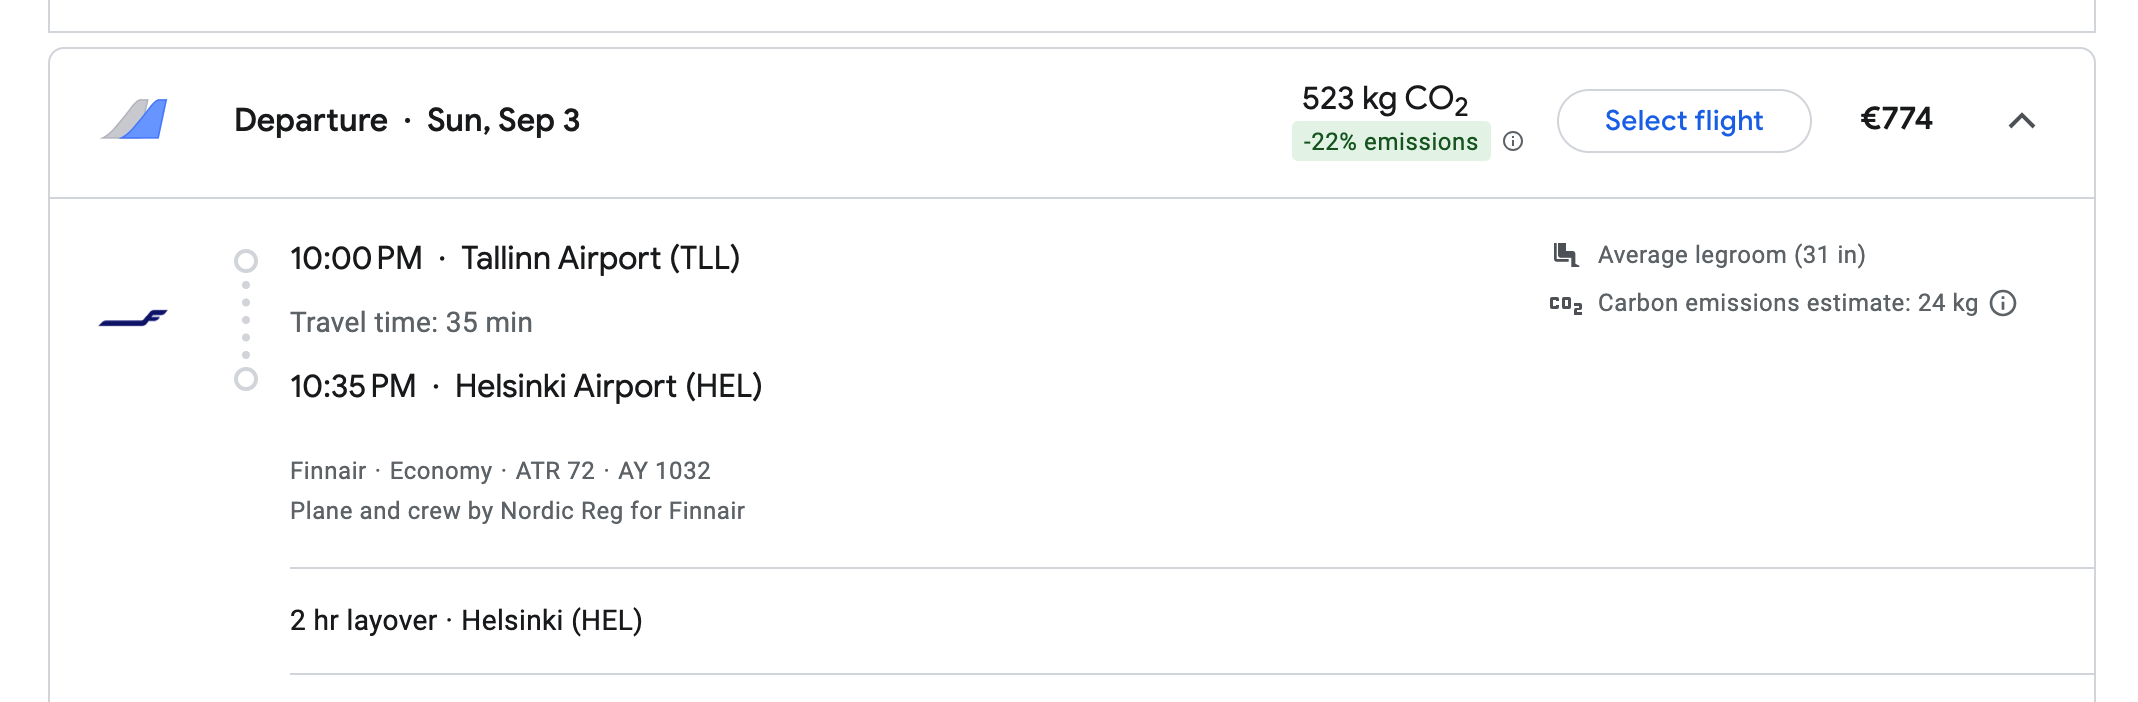
\includegraphics[width=1\textwidth,height=\textheight]{./images/design/flight-emissions.png}

}

\caption{Google's view of flight emissions}

\end{figure}%

\begin{itemize}
\tightlist
\item
  The founder of the Commons (Joro) consumer CO\textsubscript{2}
  tracking app recounts how people have a gut feeling about the 2000
  calories one needs to eat daily and daily CO\textsubscript{2} tracking
  could develop a gut feeling about one's carbon footprint (Jason
  Jacobs, 2019).
\end{itemize}

Some notable examples:

\begin{itemize}
\tightlist
\item
  Eriksson, Christensen \& Malefors (2023) discusses best practices for
  reducing food waste in Sweden.
\item
  Acuti, Lemarié \& Viglia (2023) makes the point that physical
  proximity to a drop-off point helps people participate in
  sustainability.
\item
  Wee, Choong \& Low (2021) proposes types of nudging technique based on
  an overview of 37 papers in the field.
\end{itemize}

\begin{longtable}[]{@{}
  >{\raggedright\arraybackslash}p{(\columnwidth - 2\tabcolsep) * \real{0.1786}}
  >{\raggedright\arraybackslash}p{(\columnwidth - 2\tabcolsep) * \real{0.8214}}@{}}
\caption{Types of nudge by Wee, Choong \& Low (2021)}\tabularnewline
\toprule\noalign{}
\begin{minipage}[b]{\linewidth}\raggedright
Name
\end{minipage} & \begin{minipage}[b]{\linewidth}\raggedright
Technique
\end{minipage} \\
\midrule\noalign{}
\endfirsthead
\toprule\noalign{}
\begin{minipage}[b]{\linewidth}\raggedright
Name
\end{minipage} & \begin{minipage}[b]{\linewidth}\raggedright
Technique
\end{minipage} \\
\midrule\noalign{}
\endhead
\bottomrule\noalign{}
\endlastfoot
Prompting & Create cues and reminders to perform a certain behavior \\
Sizing & Decrease or increase the size of items or portions \\
Proximity & Change the physical (or temporal) distance of options \\
Presentation & Change the way items are displayed \\
Priming & Expose users to certain stimuli before decision-making \\
Labelling & Provide labels to influence choice (for example
CO\textsubscript{2} footprint labels) \\
Functional Design & Design the environment and choice architecture so
the desired behavior is more convenient \\
\end{longtable}

\begin{itemize}
\item
  Bain et al. (2012) ``Promoting pro-environmental action in climate
  change deniers'' \textbf{(Need access!)}
\item
  Allcott (2011) ``Social norms and energy conservation'' \textbf{(Need
  access!, ncku doesn't subscribe)}
\item
  Schuitema \& Bergstad (2018) ``Acceptability of Environmental
  Policies'' \textbf{(Need access!)}
\item
  Nilsson et al. (2016) ``The road to acceptance: Attitude change before
  and after the implementation of a congestion tax'' \textbf{(Need
  access!)}
\item
  Berger, Lange \& Stahl (2022) \textbf{(Need access!)}
\item
  Anon (2022n)
\item
  United Nations Conference on Trade and Development (last) (2023)
\item
  Climatiq (2023) Automate GHG emission calculations
\item
  EarthCheck (2023) sustainable tourism certification
\item
  LFCA (2023) corporate climate action
\item
  Greenhouse Gas Protocol (2023) standards to measure and manage
  emissions
\item
  Playing for the Planet Alliance (2021)
\item
  Aka Gamification. Gamification makes uses of nudges. Students in
  Indonesia enjoy using Kahoot and it's gamification elements are
  perceived to have positive impact on individual learning outcomes so
  they are happy to continue using it (Wirani, Nabarian \& Romadhon,
  2022).
\item
  Anon (n.d.bk) game company going green
\end{itemize}

Alibaba's Ant Forest (螞蟻森林) has shown the potential gamified nature
protection, simultaneously raising money for planting forests and
building loyalty and brand recognition for their sustainable action,
leading the company to consider further avenues for gamification and
eco-friendliness.

\begin{longtable}[]{@{}
  >{\raggedright\arraybackslash}p{(\columnwidth - 6\tabcolsep) * \real{0.1585}}
  >{\raggedright\arraybackslash}p{(\columnwidth - 6\tabcolsep) * \real{0.1707}}
  >{\raggedright\arraybackslash}p{(\columnwidth - 6\tabcolsep) * \real{0.1707}}
  >{\raggedright\arraybackslash}p{(\columnwidth - 6\tabcolsep) * \real{0.4756}}@{}}
\caption{Table of Ant Forest assisted tree planting; data compiled from
(李连环 \& 姜舒译, 2017; Yang et al., 2018; UNFCCC, 2019; Wang \& Yao,
2020; Anon, 2021m; Zhang, Hu \& Gu, 2022; Wang, Ibrahiem \& Li, 2022;
Zhou, Lin \& Mou, 2023; Cao \& Liu, 2023).}\tabularnewline
\toprule\noalign{}
\begin{minipage}[b]{\linewidth}\raggedright
Year
\end{minipage} & \begin{minipage}[b]{\linewidth}\raggedright
Users
\end{minipage} & \begin{minipage}[b]{\linewidth}\raggedright
Trees
\end{minipage} & \begin{minipage}[b]{\linewidth}\raggedright
Area
\end{minipage} \\
\midrule\noalign{}
\endfirsthead
\toprule\noalign{}
\begin{minipage}[b]{\linewidth}\raggedright
Year
\end{minipage} & \begin{minipage}[b]{\linewidth}\raggedright
Users
\end{minipage} & \begin{minipage}[b]{\linewidth}\raggedright
Trees
\end{minipage} & \begin{minipage}[b]{\linewidth}\raggedright
Area
\end{minipage} \\
\midrule\noalign{}
\endhead
\bottomrule\noalign{}
\endlastfoot
2016 & ? & 0 & \\
2017 & 230 million & 10 million & \\
2018 & 350 million & 55 million & 6500 acres?? \\
2019 & 500 million & 100 million & 112,000 hectares / 66, 000
hectares? \\
2020 & 550 million & 200 million & 2,7 million acres? \\
2021 & 600 million & 326 million & \\
2022 & 650 million & 400 million & 2 million hectares \\
& & & \\
& & & \\
\end{longtable}

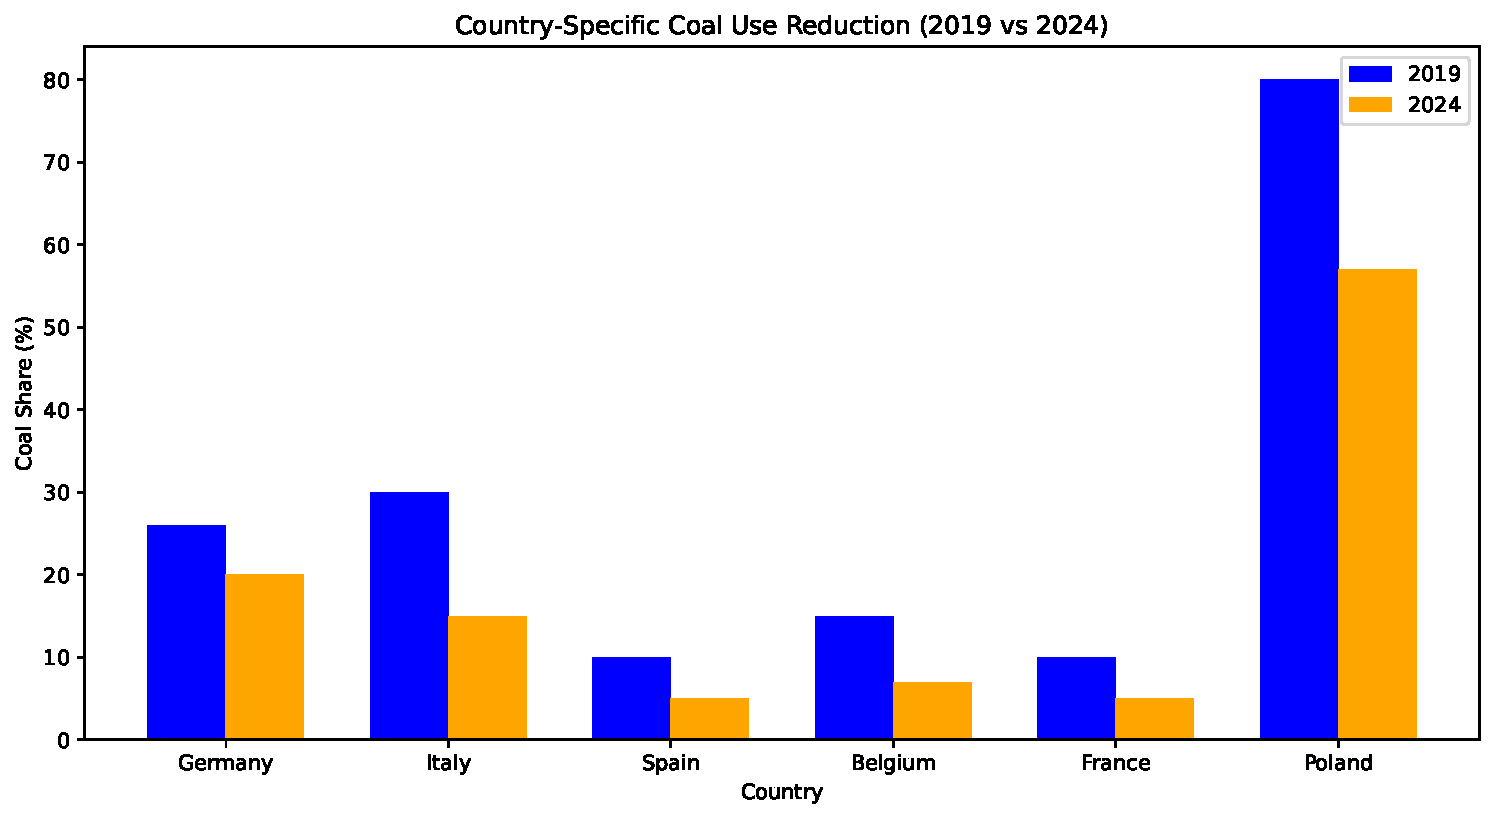
\includegraphics{_thesis_files/figure-pdf/cell-26-output-1.pdf}

\subsubsection{Open Data Sharing}\label{open-data-sharing}

Open Data Enables Collaboration

\begin{itemize}
\tightlist
\item
  Taiwan is a proponent of Open Gov OP-MSF OGP (Open Government
  Partnership, 2021; Lab, 2021)
\end{itemize}

Data-driven design requires access to data. making the movement towards
\emph{open data sharing} very important. Some countries and cities are
better than others at sharing data openly.

\begin{longtable}[]{@{}lll@{}}
\caption{Examples of cities and countries that share data
openly.}\tabularnewline
\toprule\noalign{}
Country & Project & Reference \\
\midrule\noalign{}
\endfirsthead
\toprule\noalign{}
Country & Project & Reference \\
\midrule\noalign{}
\endhead
\bottomrule\noalign{}
\endlastfoot
Sweden & Swedish open data portal & Anon (n.d.bn) \\
& & \\
& & \\
\end{longtable}

\begin{itemize}
\tightlist
\item
  When will Bolt show CO\textsubscript{2} emissions per every trip?
\item
  Sustainable finance data platform:
\item
  WikiRate (2021) WikiRate defines Data Sharing Archetypes
\end{itemize}

\begin{longtable}[]{@{}
  >{\raggedright\arraybackslash}p{(\columnwidth - 2\tabcolsep) * \real{0.3786}}
  >{\raggedright\arraybackslash}p{(\columnwidth - 2\tabcolsep) * \real{0.6214}}@{}}
\toprule\noalign{}
\begin{minipage}[b]{\linewidth}\raggedright
Type
\end{minipage} & \begin{minipage}[b]{\linewidth}\raggedright
Example
\end{minipage} \\
\midrule\noalign{}
\endhead
\bottomrule\noalign{}
\endlastfoot
Transparency Accountability Advocate & \\
Compliance Data Aggregator & \\
Data Intelligence Hub & \\
Worker Voice Tool & Caravan Studios (2022): \textbf{``Worker
Connect''} \\
Traceability tool & trustrace.com \\
Open data platform & \\
Knowledge sharing platform & business-humanrights.org \\
\end{longtable}

\begin{itemize}
\tightlist
\item
  WikiRate is a tool for checking green credentials Transparency
\item
  Laureen van Breen et al. (2023)
\item
  Wikirate (2022a)
\item
  Anon (n.d.af)
\item
  Ray (2023) comprehensive overview of Web3.
\item
  Rehash: A Web3 Podcast (2022) human-centered web3
\end{itemize}

\subsubsection{Data Privacy}\label{data-privacy}

Sustainability needs to be balanced with privacy.

\begin{itemize}
\tightlist
\item
  Sanchez et al. (2022) suggests tracking users using their smartphones
  and attributing points for actions deemed beneficial yet this has
  potentially privacy issues.
\end{itemize}

\subsection{Self-Monitoring}\label{self-monitoring}

Research on \emph{personal data tracking} also known as \emph{quantified
self} or \emph{self-monitoring} is abundant. Wearable devices including
the Apple Watch, Oura Ring, Fitbit and others, combined with apps, help
users track a variety of health metrics. Apart from health, wearable
devices have been used to track other metrics such as physiological
parameters of students at school to determine their learning efficiency
(Giannakos et al., 2020). Not only can health metrics be tracking, but
exposure to pollution as well as personal carbon footprint, are all to
some extent trackable (if not traceable).

\subsubsection{Carbon Tracking}\label{carbon-tracking}

Personal carbon footprint tracking apps (aka CO2 calculators) in a
mid-sized German city (N=216) helped overall emission reduction by 23\%
correlating with feedback from the app specifically reducing emissions
from heating 26.9\%, food 16.4\%, household 34.7\% reduction, and
mobility 12\%(Hoffmann et al., 2024).

We have a limited carbon budget so calculating CO2e-cost become
integrated into every activity.

\begin{itemize}
\item
  CO2e calculations will be part of our everyday experience
\item
  Zhang's Personal Carbon Economy conceptualized the idea of carbon as a
  currency used for buying and selling goods and services, as well as an
  individual carbon exchange to trade one's carbon permits (Zhang,
  2018).
\end{itemize}

Personal Carbon Trackers

Personal carbon footprint calculators have been released online, ranging
from those made by governments and companies to student projects.
Similar to personal health trackers, personal CO\textsubscript{2}
trackers help one track emissions and suggests sustainable actions.

\begin{longtable}[]{@{}
  >{\raggedright\arraybackslash}p{(\columnwidth - 2\tabcolsep) * \real{0.3133}}
  >{\raggedright\arraybackslash}p{(\columnwidth - 2\tabcolsep) * \real{0.6867}}@{}}
\caption{A selection of personal sustainability apps. See
\emph{greenfilter.app} for an updated database.}\tabularnewline
\toprule\noalign{}
\begin{minipage}[b]{\linewidth}\raggedright
App
\end{minipage} & \begin{minipage}[b]{\linewidth}\raggedright
Description
\end{minipage} \\
\midrule\noalign{}
\endfirsthead
\toprule\noalign{}
\begin{minipage}[b]{\linewidth}\raggedright
App
\end{minipage} & \begin{minipage}[b]{\linewidth}\raggedright
Description
\end{minipage} \\
\midrule\noalign{}
\endhead
\bottomrule\noalign{}
\endlastfoot
Commons (Formerly Joro) & Finacial Sustainability Tracking + Sustainable
Actions \\
Klima & Offset Subscription \\
Wren & Offset Subscription \\
JouleBug & \\
eevie & \\
Aerial & \\
EcoCRED & \\
Carbn & \\
LiveGreen & \\
Earth Hero & \\
& \\
\end{longtable}

\subsubsection{Pollution Exposure
Tracking}\label{pollution-exposure-tracking}

My personal air pollution exposure tracked using the Atmotube device
attached to my backpack. Tracking air pollution and realizing how bad
the over in my grandma's house is: add picture. Quantified Self is an
example of Digital Health. There is a parallel in health to
sustainability and indeed both are inextricably linked. Open Source code
for calculating air pollution exposure AQI (Atmotech, 2024).

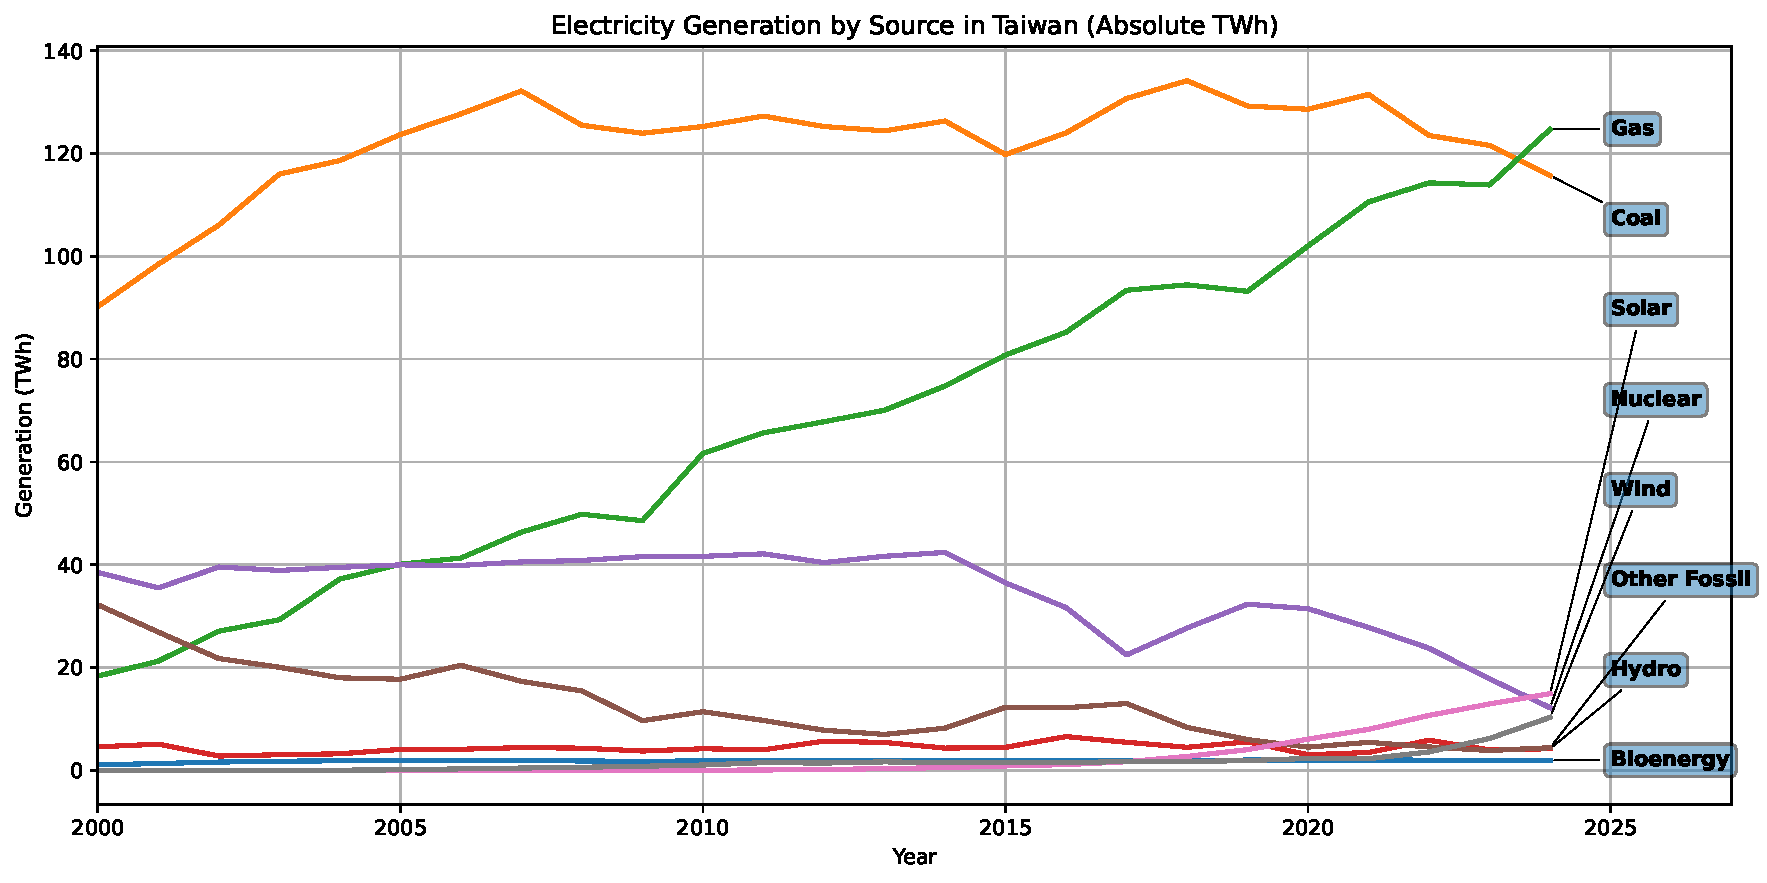
\includegraphics{_thesis_files/figure-pdf/cell-27-output-1.pdf}

\subsubsection{\texorpdfstring{\textbf{Health and Fitness
Tracking}}{Health and Fitness Tracking}}\label{health-and-fitness-tracking}

EEG (electroencephalogram), ECG (Electrocardiogram), EDA (Electrodermal
Activity): tracking features of brain, heart and nervous system
activity. Brain Music Lab founder and brain researcher Grace Leslie:
``brain music sounds like a warm bathtub''. Tracking blood sugar with
app and patches. Blood sugar trackers. Blood glucose tracking is popular
even for people without diabetes, to optimize their activity (Anon,
2021k). Tracking urine consistency inside your toilet with WithThings.
Companies like NeuralLink are building devices to build meaningful
interactions from brain waves (EEG).

Apple is a leader in health tracking. In 2022 Apple outlined plans for
\emph{``empowering people to live a healthier day''} and Apple's
HealthKit provides a growing list of health metrics, which app
developers can tap into (Apple, 2022a, 2022b). Liu et al. (2019) tracks
how wearable data is used for tracking sleep improvements from exercise.
Grigsby-Toussaint et al. (2017) made use of sleep apps to construct
humans behaviors also known as \emph{behavioral constructs}. The Oura
ring is an example of \emph{calm technology}, providing helpful data
without calling an attention to itself (Phelan, 2024).

Use technology Wearables to be more aware of one's health. Example of
quantified self device.

fitness metrics

Could one track personal sustainability in a similar fashion? (Shin et
al., 2019)'s synthesis review of 463 studies shows wearable devices have
potential to influence behavior change towards healthier lifestyles.
Saubade et al. (2016) finds health tracking is useful for motivating
physical activity. The urban environment has an influence on health.

While so of the behavior changes may sound simple - like switching from
driving to walking - and would have a large environmental effect, they
are hindered by factors from personal motivation to (lack of) suitable
urban architecture. (Delclòs-Alió et al., 2022) discusses walking in
Latin-American cities. Walking is the most sustainable method or
transport but requires the availability of city infrastructure, such as
sidewalks, which many cities still lack.

Personal data enables behavior change.

While the scale of climate change is too big for individual action to
make a difference, individual action can foster hope and a sense of
collective responsibility (Nature, 2020).

\begin{itemize}
\item
  Kristian Steensen Nielsen (2022) \textbf{Individual climate action!!!}
\item
  The UN has been handing out Global Climate Action Awards since 2011
  for idea such as the Climate Credit Card in Switzerland, which
  automatically tracks emissions of purchases, creates emissions'
  reports for the user which can then be offset with investments in
  climate projects around the world (UNFCCC, 2023a).
\item
  Give Gen-Z the tools to turn climate anger into positive change to
  transform companies
\item
  Echeverría, Gimenez-Nadal \& Molina (2022) suggests greener modes of
  mobility.
\item
  Anon (2017b)
\item
  Brantley (2021)
\item
  Contact Kalle Lasn, Culture Jam
\item
  ``ESG Accessibility'', Large-scale accessibility to ESG,
\item
  increase ESG accessibility
\item
  Shop sustainability in Estonia (Lilleväli, 2022; Anon, n.d.v).
  Tarbimise jalajälg poes (Helen Saarmets, 2021). Offsets at the point
  of sale (Anon, n.d.ad).
\item
  Green Finance Platform (2020) report predicts the rise of
  personalizing sustainable finance, because of its potential to grow
  customer loyalty, through improving the user experience. Similarly to
  good design, interacting with sustainable finance for the
  `green-minded' demographics, providing a reliable green product is a
  way to build customer loyalty.
\end{itemize}

Another aspect is tracking one's mental health. (Tyler, Boldi \&
Cherubini, 2022) surveys the use of self-reflection apps in the UK
(n=998).

\begin{itemize}
\tightlist
\item
  Popular Strava (100+ million users) sports assistant provides run
  tracking and feedback (Strava, 2022).
\end{itemize}

\begin{figure}[H]

{\centering 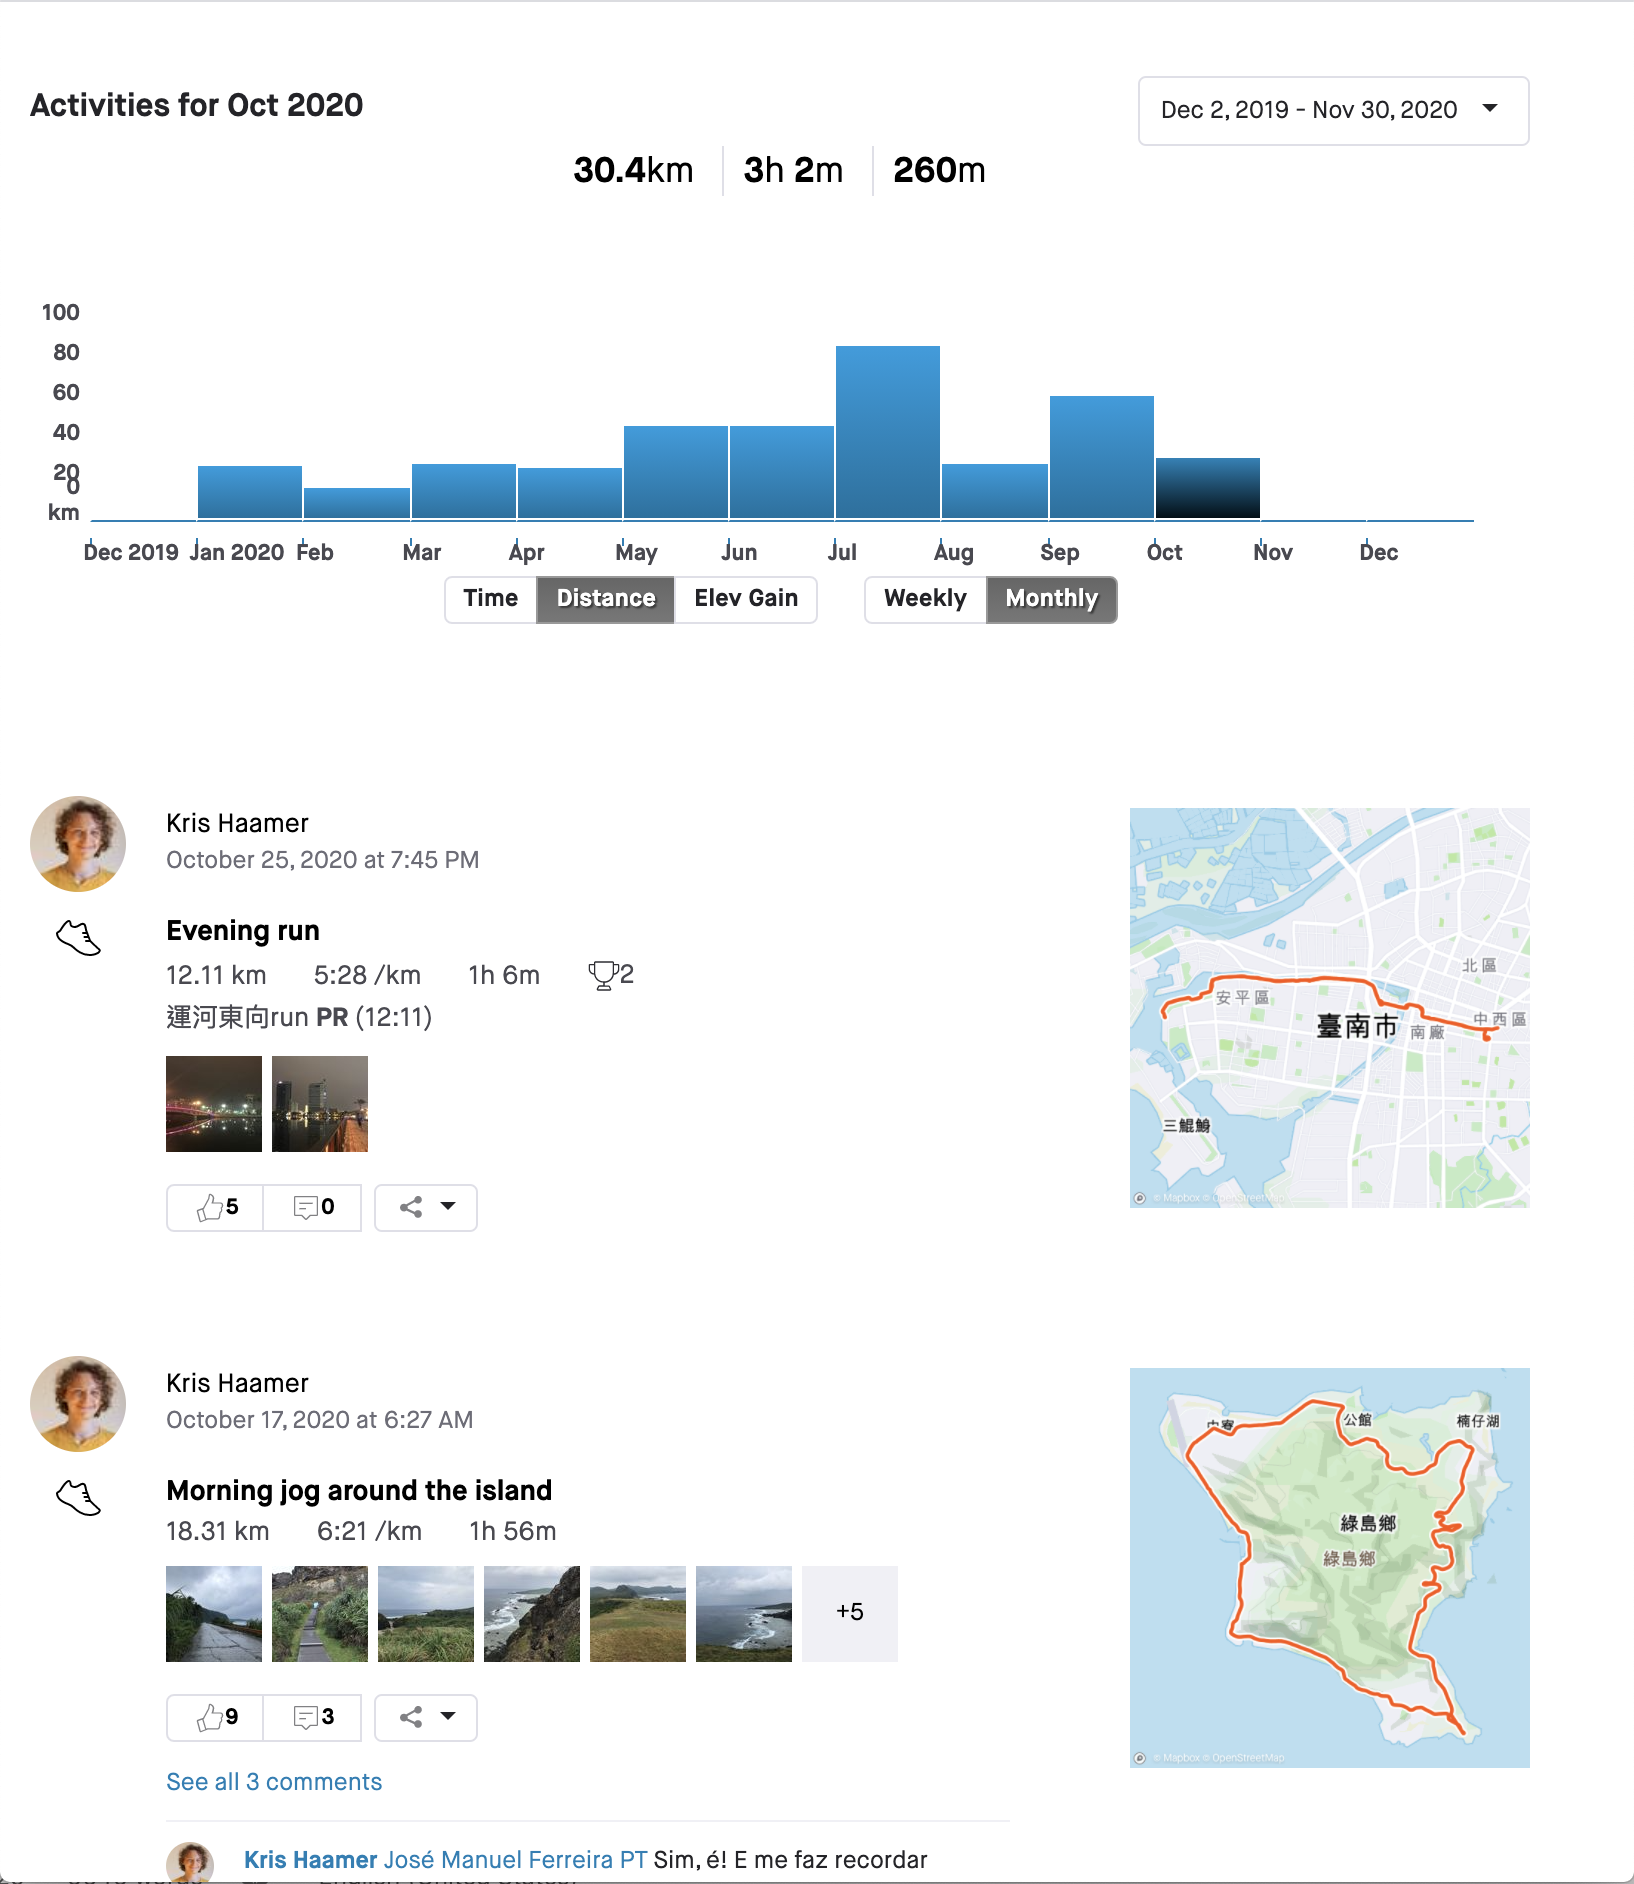
\includegraphics[width=1\textwidth,height=\textheight]{./images/design/strava.png}

}

\caption{Popular Strava sports assistant provides run tracking and
feedback}

\end{figure}%

\begin{itemize}
\item
  AI Financial Advisors will need to go further to motivate users.
\item
  DBS digibank app added a financial advisor named ``Your Financial
  GPS'' in 2018 DBS (2018)
\item
  ``urban metabolism'' (Anon, 2021s; Claire Moran, 2018), city in-out
  flows accounting method
\item
  Tsai et al. (2019)
\item
  Burger, White \& Yearworth (2019)
\item
  Aromatario et al. (2019) behavior changes
\item
  Ayoola et al. (2018) wellbeing data
\item
  Godfrey et al. (2018)
\item
  Thomas et al. (2018)
\item
  Tonne et al. (2017)
\item
  Anselma, Mazzei \& De Michieli (2017)
\item
  Forlano (2017) post-humanism and design
\item
  Greenbaum \& Gerstein (2016)
\item
  Millings et al. (2015)
\item
  Reis et al. (2015)
\item
  Bower \& Sturman (2015)
\item
  Fletcher (2022)
\item
  Ryan (2022) uses the ``capability methodology'' to evaluate if apps
  help people eat healthily.
\item
  Baptista et al. (2022) apps for sleep apnea
\end{itemize}

The small screen estate space of mobiles phones and smart watches
necessitates displaying content in a dynamic manner. Virtual reality
glasses (called AR/VR or XR in marketing speak) need dynamic content
because the user is able to move around the environment. These are
questions that interaction design is called upon to solve. Hoang (2022):
\emph{``Dynamic interfaces might invoke a new design language for
extended reality''.}

Speaking is one mode of interaction that's become increasingly possible
as machines learn to interpret human language.

\begin{longtable}[]{@{}ll@{}}
\caption{Modes of interaction}\tabularnewline
\toprule\noalign{}
Mode of Interaction & \\
\midrule\noalign{}
\endfirsthead
\toprule\noalign{}
Mode of Interaction & \\
\midrule\noalign{}
\endhead
\bottomrule\noalign{}
\endlastfoot
Writing & \\
Speaking & \\
Touching & \\
Moving & \\
& \\
\end{longtable}

\subsection{Re-Designing Industries for
Circularity}\label{re-designing-industries-for-circularity}

Circular Economy

We're in an industrial revolution. Many companies are investing into
transforming their processes. \emph{``{[}T{]}ransition to a low carbon
economy presents challenges and potential economic benefits that are
comparable to those of previous industrial revolutions''} (Pearson \&
Foxon, 2012). It's possible to re-design entire industries and that is
exactly the expectation sustainability sets on businesses. Across all
industries, there's a call for more transparency. Conversations about
sustainability are too general and one needs to look at the specific
sustainability metrics at specific industries to be able to design for
meaningful interaction. There's plentiful domain-specific research
showing how varied industries can develop eco-designed products. I will
here focus on 3 industries that are relevant for college students.

Food and clothes (I'm omitting housing and transport here) are part of
the immediate environmental impact of college students.

\begin{itemize}
\tightlist
\item
  5th industrial revolution, advanced robotics
\item
  6th industrial revolution, quantum computing, nanotechnology Chourasia
  et al. (2022)
\item
  7th industrial revolution futurists are looking at current trends and
  building scenarios for 2050 envisioning a world where the convergence
  of bio-based and mineral-based technologies, widespread sustainability
  and energy-abundance (Ruiz Estrada, 2024).
\end{itemize}

\ldots for Provenance and Traceability

Companies like Qima provide inspection and certification services QIMA
(2024)

\subsubsection{Circular Economy}\label{circular-economy}

Circular economy is a tiny part of the world economy. (Circle Economy,
2022) reports only 8.6\% of world economy is circular and \emph{100B
tonnes of virgin materials} are sourced every year.

Encouraging Sustainable Design and Reducing Waste.

(Liu et al., 2023b) reports, e-waste is growing 3\%-5\% every year,
globally. (Thukral \& Singh, 2023) identifies several barriers to
e-waste management among producers including lack of awareness and
infrastructure, attitudinal barriers, existing \emph{informal} e-waste
sector, and the need for an e-waste license.

\begin{itemize}
\item
  McDonough \& Braungart (2002) from Cradle to Grave book was released
  over 2 decades ago, change is slow.
\item
  McGinty (Thu, 08/06/2020 - 11:25): How to Build a Circular Economy
\item
  Dull (2021) book, many current technological hurdles can be overcome
  by supply chain professionals who are experts in connecting supply
  streams.
\end{itemize}

also known as circular economy. Assuming that as individuals we want to
act in a sustainable way, how exactly would be go about doing that?

\ldots for Sustainable Products

How can design enable/help/encourage sustainability?

\begin{itemize}
\item
  Use imagination
\item
  Societal movements change things: implication for design: build a
  community
\item
  Growing public understanding of how nature works and intersects with
  our use of money.
\item
  Hedberg \& Šipka (2021) argues digitization and data sharing is a
  requirement for building a circular economy.
\item
  ``Circular Petrochemicals'' Lange (2021)
\item
  Supply chain transparency enables stakeholder accountability
  (Circularise, 2018; Doorey, 2011; Fox, 2007).
\item
  Recycling Critical Raw Materials, digitization of mining allows
  enhance the reliability of supply chains (CRM Alliance, 2020).
\item
  EIT RawMaterials
\end{itemize}

\subsubsection{Case: Fast-Moving Consumer Goods
(FMCG)}\label{case-fast-moving-consumer-goods-fmcg}

Fast-Moving Consumer Goods (FMCG) also known as Consumer Packaged Goods
(CPG) are large global congloremates operating with low margins and high
volumes (Toh, 2024). The largest of them have several billions in
revenue (Kenton, 2024).

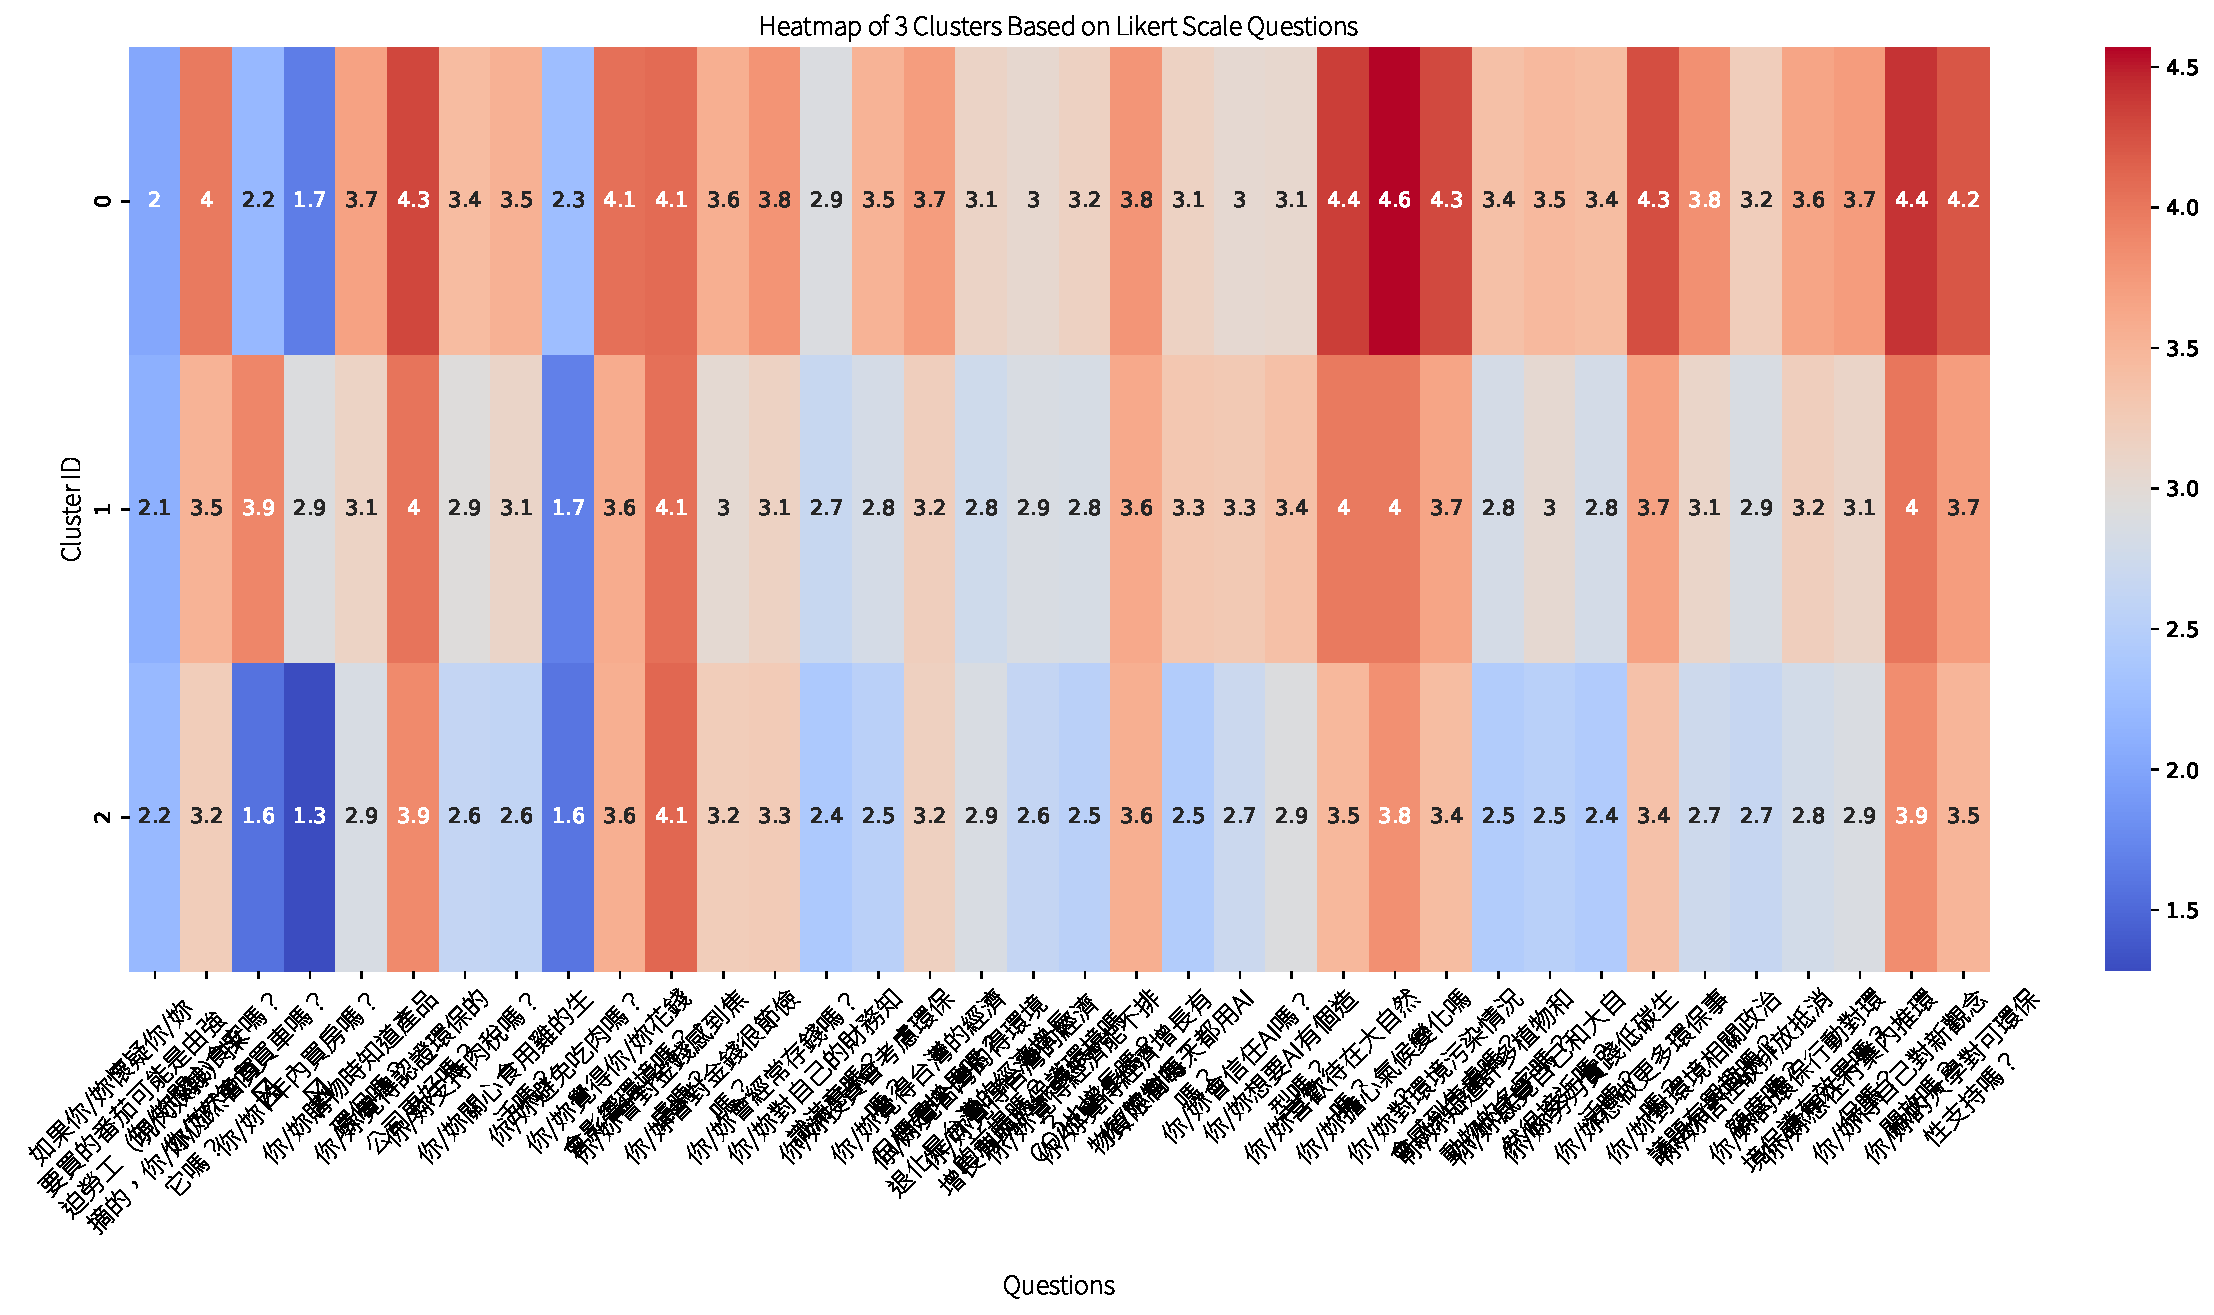
\includegraphics{_thesis_files/figure-pdf/cell-28-output-1.pdf}

Rise of e-commerce has pushed logistics companies to increase delivery
efficiency to keep up with FMCG sales (Deliverect, 2024).

\subsubsection{Case: Fashion}\label{case-fashion}

Just like Fast-Moving Consumer Goods, fast fashion operates with low
margins and follows consumer trends. Young people are the largest
consumers of fast fashion (Anon, n.d.bx). (In European Environment
Agency, 2022 European Environment Agency (EEA)) estimates based on trade
and production data that EU27 citizens consumed an average 15kg of
textile products per person per year. The European Commission wants to
reduce the impact of fast fashion on EU market (ERR, 2022).
(Millward-Hopkins, Purnell \& Baurley, 2023) shows how 50\% of the
textile waste in the UK is exported to other countries.

``26 million tons of clothing end up in China's landfills each year,
propelled by fast fashion'' (Tian Macleod Ji, 2024).

Greenwashing is prevalent in the fashion industry. \textbf{Problem}:
Emily Chan (2022a) report says there's not enough transparency in
fashion. Fashion Revolution Foundation (2022) Fashion transparency
index. (Wikirate, 2022b): ``Among the Index's main goals are to help
different stakeholders to better understand what data and information is
being disclosed by the world's largest fashion brands and retailers,
raise public awareness, educate citizens about the social and
environmental challenges facing the global fashion industry and support
people's activism''. Consumer understanding of sustainability is
limited. Mabuza, Sonnenberg \& Marx-Pienaar (2023) shows consumer
knowledge of apparel coloration is very limited.

2.4 Trillion USD fashion industry contributing 2\%-8\% of total global
GHG emissions, 100B USD lost to lack of recycling, contributes 9\% of
microplastics (Adamkiewicz et al., 2022). (Centobelli et al., 2022)
Fashion industry year uses 9B cubic meters of water, 1.7B tonnes of
CO\textsubscript{2}, 92 million tonnes of textile waste. Köhler et al.
(2021) Globally 87\% of textile products are burned or landfilled after
1st consumer use.

\paragraph{Towards Sustainable
Clothes}\label{towards-sustainable-clothes}

\begin{itemize}
\item
  There are local policy initiatives aiming to tackle the waste problem.
  For example the New Standard Institute's proposed ``Fashion Act'' to
  require brands doing business in New York City to disclose
  sustainability data and set waste reduction targets (Emily Chan,
  2022b) .
\item
  (Leung \& Luximon, 2021) There's a growing know-how on how to produce
  sustainably and which materials to use. ``Handbook of Footwear Design
  and Manufacture'' Chapter 18~-~Green design. Industry collaboration
  can raise the bar for everyone, such as the Better Cotton Initiative
  (Better Cotton, 2023).
\item
  Story of Patagonia (Chouinard, 2005){]}.
\end{itemize}

Sustainable Fashion, Textile Design

\begin{itemize}
\tightlist
\item
  There are signs of young Chinese consumers valuing experiences over
  possessions (Jiang, 2023).
\end{itemize}

Across industries, reports are saying there isn't enough transparency.

\begin{itemize}
\item
  (Hannah Ritchie, 2020; US EPA, 2016) GHG emission inventory by sector
\item
  Marrucci, Marchi \& Daddi (2020) Italian retail supermarkets carbon
  footprint?
\item
  Gyabaah et al. (2023) research across several dumpsites across Ghana
  revealed up to 12\% of the landfill consisted of textile waste.
\item
  imperfectidealist (2020) Fashion sustainability vs greenwashing
\item
  Anon (2023ah) Ethical Shopping
\item
  Anon (2023ad) Ethical brand?
\item
  Good On You (2023) Sustainable fashion company evaluations
\item
  Anon (n.d.aq) Garment Worker's rights
\item
  Emily Chan (2022c): fashion companies can't be held accountable for
  their actions (or indeed, their lack of action).
\item
  WikiRate (2023)
\item
  Anon (2022h): ``Political consumerism'', ``Instant Gratification for
  Collective Awareness and Sustainable Consumerism''
\item
  FashionChecker (2023)
\item
  Eesti Disainikeskus I Estonian Design Centre (2021) Circular textiles
\item
  Eesti Kunstiakadeemia (2022) Sustainable Fashion education
\item
  Anon (n.d.k)
\item
  ``The mainstream fashion industry is built upon the exploitation of
  labor, natural resources and the knowledge of historically
  marginalized peoples.''
\item
  Anon (n.d.bo)
\item
  ``Secrecy is the linchpin of abuse of power\ldots its enabling force.
  Transparency is the only real antidote.'' Glen Greenwald, Attorney and
  journalist.
\item
  Stand.earth (2023)
\item
  Anon (n.d.av)
\item
  Anon (n.d.g) Bangladesh Garment Manufacturers and Exporters
  Association
\item
  Minimize shopping, buy quality, save CO\textsubscript{2}, invest.
\item
  Textile Exchange (2023) Ethical fashion materials matter
\item
  Textile Exchange (2021): Policy request
\item
  Free clothes
\item
  Vanish UK (2021) ``Generation rewear'' documentary, sustainable
  fashion brands
\item
  Storbeck (2021) and Remington (2020): Zalando says Fast fashion must
  disappear
\item
  Infinited Fiber (2023)
\item
  Cleantech Group (2023) Global cleantech 100
\item
  Anon (2023ae) Alterations and repairs made easy
\item
  Anon (2023l) Ethical brand ratings
\end{itemize}

\subsubsection{Case: Food}\label{case-food}

Re-designing industrial food systems for an increasing global population
is a challenge. Supply chain innovation in food industries may enable
more transparency. \textbf{provenance and traceability of food has
implications for sustainability and health.}

Global warming leading to droughts and extreme weather, wars and
conflicts increased volatility in food prices (Eshe Nelson, Ana Swanson
\& Jeanna Smialek, 2023).

``The agricultural sector contributes to approximately 13.5\% of the
total global anthropogenic greenhouse gas emissions and accounts for
25\% of the total CO\textsubscript{2} emission'' (Nabipour Afrouzi et
al., 2023). Poore \& Nemecek (2018) suggests 26\% of carbon emissions
come from food production. Saner et al. (2015) reports dairy (46\%) and
meat and fish (29\%) products making up the largest GHG emission
potential. Springmann et al. (2021) proposes veganism is the most
effective decision to reduce personal CO\textsubscript{2} emissions.

\emph{Farm to Fork} is a European Union policy to shorten the supply
chain from the producer to the consumer and add transparency to the
system. Patel et al. (2023) livestock products (meat) are 15\% of
agricultural foods valued at €152 billion in 2018 globally.

\begin{itemize}
\item
  Farm to Fork Financial Times (2022)
\item
  Fake honey, DNA-analysis to find real honey, synthetic honey can pass
  laboratorty tests (ERR, 2023)
\item
  China is the largest honey producer.
\item
  Food fraud
\end{itemize}

Anon (n.d.bm)

Anon (n.d.az) app for nutrition and sustainability data

\textbf{Fishing}

\begin{itemize}
\item
  75\% of fishing is done using industrial Trawling, which has
  environmental impact
\item
  Bailey \& Eggereide (2020) shows how the Norwegian government plans to
  increase salmon production 5x by 2050. How can this be sustainable?
  Mostly this means fish-farming
\item
  Complex supply chains make seafood (marine Bivalvia, mollusks)
  logistics prone to fraud, leading to financial losses and threats to
  consumer health (Santos et al., 2023). (Chang et al., 2021) \emph{fish
  fraud} is a large global problem but it's possible to use DNA-tracking
  to prove where the fish came from. In ``2019, the 27 KURA SUSHI
  branches in Taiwan sold more than 46 million plates of sushi. in
  Taiwan''. Illegal, unreported and unregulated fishing (IIU) fishing is
  widespread; the EU is adopting countermeasures (Kim \& Lim, 2024).
  Muñoz et al. (2023) Is there such a thing as sustainable fishing?
  Bottom trawling is the worst and should be banned. Katie Gustafson
  (2022) proposes a \textbf{``Uniform traceability system for the entire
  supply chain''} for seafood. Mamede et al. (2022) proposes
  \emph{Seafood tracing}: Fingerprinting of Sea Urchin.
\item
  The same is true for cocoa beans, which are at risk from food fraud
  (Fanning et al., 2023).
\item
  \textbf{Perennial Crops,} Multi-year crops reduce inputs of gasoline,
  labor, etc. (Aubrey Streit Krug \& Yin Lu, 2023). Large agritech
  companies like Monsanto rely on selling seeds annually for profits
  putting them at odds with \textbf{Perennial crops}. Single-year seeds
  have led to farmer suicides when crops fail in poor communities.
\item
  Sustainability Accounting Standards Board, part of the International
  Financial Reporting Standards Foundation
\item
  Global Reporting Iniative
\item
  Anon (2022m)
\item
  Anon (2021n) ``Real Time ESG Tracking From StockSnips''
\item
  Waters (2015) \textbf{(Need access!)}
\item
  Cawthorn \& Hoffman (2016) \textbf{(Need access! ncku doesn't
  subsribe)}
\item
  Gamborg \& Jensen (2017) \textbf{(Need access!)}
\item
  Neethirajan \& Kemp (2021) using biometric sensors to track livestock
  sustainability.
\item
  Inc (n.d.)
\item
  Tim Nicolle (2017)
\item
  EAT-Lancet diet
\end{itemize}

\textbf{Culture, Community, Cuisine, Storytelling}

\begin{itemize}
\tightlist
\item
  Tsing (2015) mushrooms
\item
  Food is about enticing human imagination and taste buds. Potato used
  to be a newcomer and innovative crop in Europe, and now it's so
  common, Europeans forget it's no originally from Europe. Food is also
  about cuisine and culture; foods become popular if we hear stories and
  see cuisine around a particular crop (Aubrey Streit Krug \& Yin Lu,
  2023).
\item
  IARC warns aspartame (artificial sweetener found in many soft drinks)
  could cause cancer {[}ADD CITATION{]}.
\item
  Yap et al. (2023) Singapore disposes of 900,000 tonnes of plastic
  waste out of which only 4\% is recycled.
\item
  Kiessling et al. (2023) Single-use plastics make up 44-68\% of all
  waste mapped by citizen scientists.
\end{itemize}

\textbf{Food Waste}

There are several initiatives to reduce food waste by helping people
consume food that would otherwise be throw away.

\begin{figure}[H]

{\centering 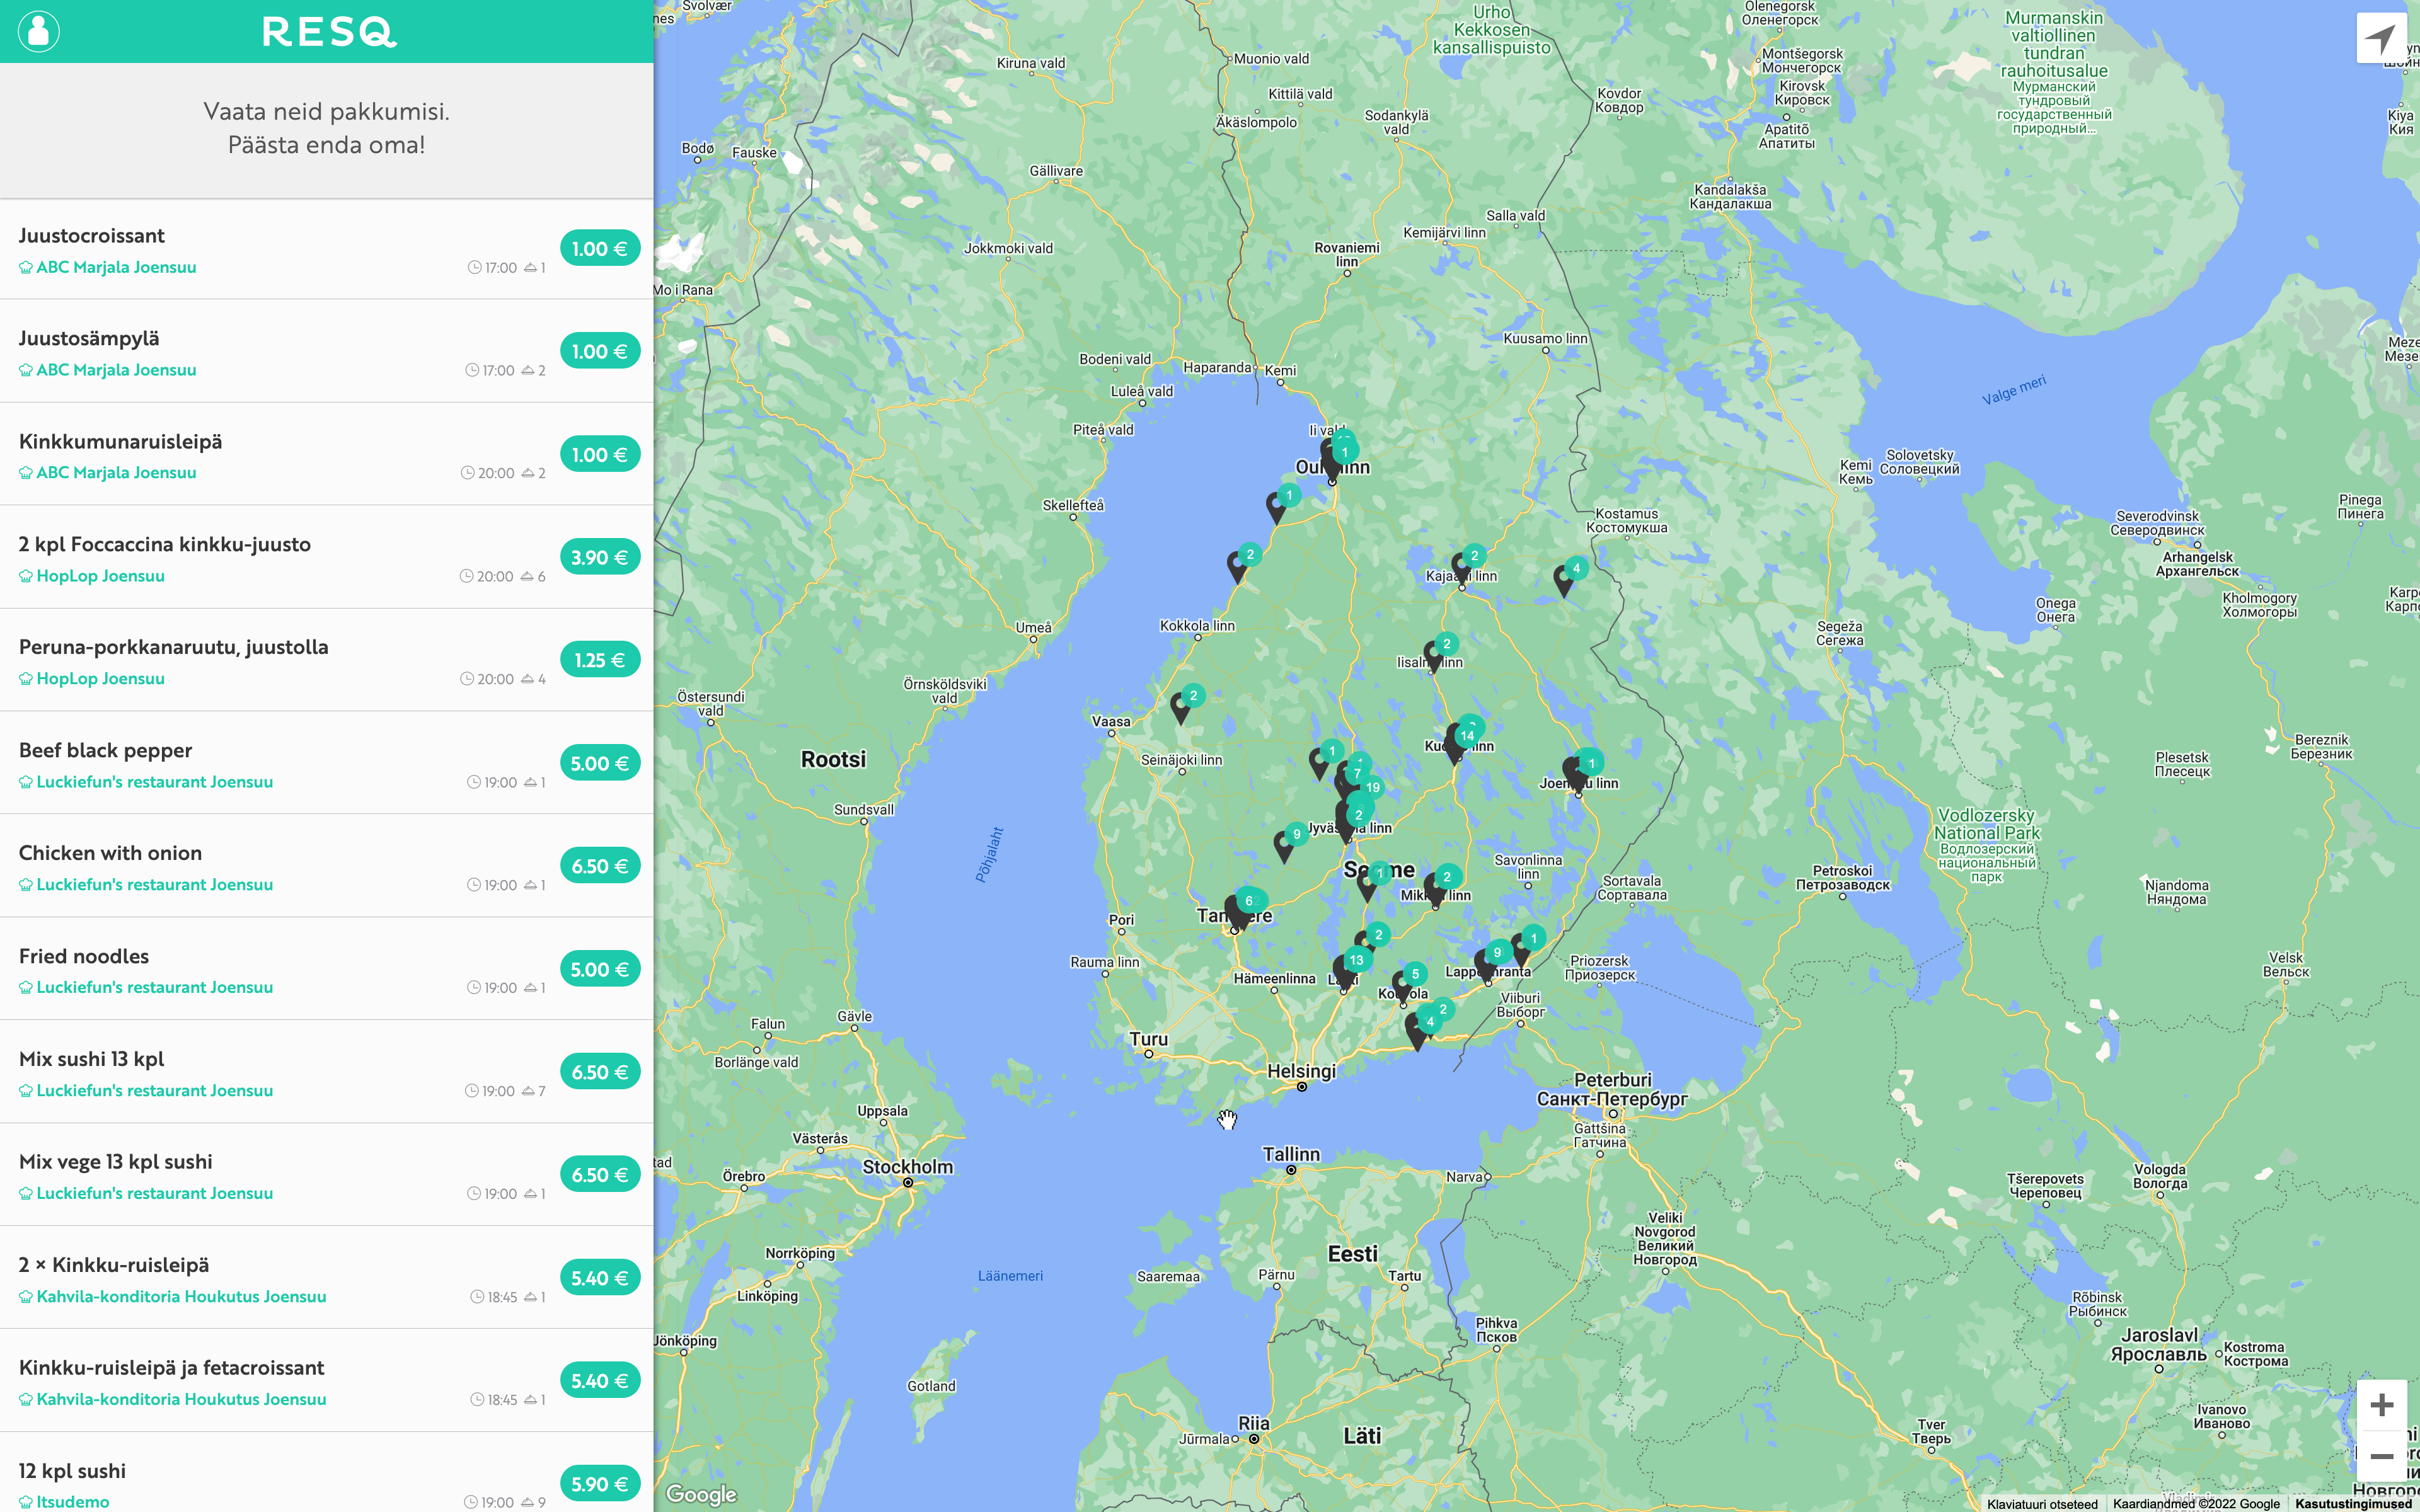
\includegraphics[width=1\textwidth,height=\textheight]{./images/design/resq-club.png}

}

\caption{ResQ Club saves food waste by selling left-over foods cheaply}

\end{figure}%

\begin{longtable}[]{@{}
  >{\raggedright\arraybackslash}p{(\columnwidth - 2\tabcolsep) * \real{0.1469}}
  >{\raggedright\arraybackslash}p{(\columnwidth - 2\tabcolsep) * \real{0.8531}}@{}}
\caption{Food saving apps}\tabularnewline
\toprule\noalign{}
\begin{minipage}[b]{\linewidth}\raggedright
Name
\end{minipage} & \begin{minipage}[b]{\linewidth}\raggedright
\end{minipage} \\
\midrule\noalign{}
\endfirsthead
\toprule\noalign{}
\begin{minipage}[b]{\linewidth}\raggedright
Name
\end{minipage} & \begin{minipage}[b]{\linewidth}\raggedright
\end{minipage} \\
\midrule\noalign{}
\endhead
\bottomrule\noalign{}
\endlastfoot
Karma & \\
ResQ Club & (Kristina Kostap, 2022) ResQ Club in Finland and Estonia for
reducing food waste by offering a 50\% discount on left-over restaurant
meals before they are thrown away. \\
Kuri & Haje Jan Kamps (2022) Less impact of food \\
Social media groups (no app) & \\
\end{longtable}

\begin{itemize}
\tightlist
\item
  Röös et al. (2023) identified 5 perspectives in a small study
  (\emph{n=106}) of views on the Swedish food system:
\end{itemize}

\begin{longtable}[]{@{}
  >{\raggedright\arraybackslash}p{(\columnwidth - 2\tabcolsep) * \real{0.3016}}
  >{\raggedright\arraybackslash}p{(\columnwidth - 2\tabcolsep) * \real{0.6984}}@{}}
\caption{Perspective on food systems in Sweden.}\tabularnewline
\toprule\noalign{}
\begin{minipage}[b]{\linewidth}\raggedright
Perspective
\end{minipage} & \begin{minipage}[b]{\linewidth}\raggedright
Content
\end{minipage} \\
\midrule\noalign{}
\endfirsthead
\toprule\noalign{}
\begin{minipage}[b]{\linewidth}\raggedright
Perspective
\end{minipage} & \begin{minipage}[b]{\linewidth}\raggedright
Content
\end{minipage} \\
\midrule\noalign{}
\endhead
\bottomrule\noalign{}
\endlastfoot
\emph{``The diagnostic perspective''} & ``\emph{All hands on deck to fix
the climate''} \\
\emph{``The regenerative perspective''} & ``\emph{Diversity, soil health
and organic agriculture to the rescue''} \\
\emph{``The fossil-free perspective''} & ``\emph{Profitable Swedish
companies to rid agriculture and the food chain of fossil fuel''} \\
\emph{``The consumer-driven perspective''} & \emph{``A wish-list of
healthy, high-quality and climate-friendly foods''} \\
``The hands-on perspective'' & ``Tangible solutions within the reach of
consumers and the food industry'' \\
\end{longtable}

\begin{itemize}
\item
  ``regenag'', Václav Kurel, we need help consumers demand regenerative
  agriculture Baltic Sea Action Group (2023)
\item
  Kommenda et al. (2022) Carbon Food Labels
\item
  Food Sovereignty: ``The global food sovereignty movement, which had
  been building momentum since its grassroots conception in the late
  '90s, quickly gained traction with its focus on the rights of people
  everywhere to access healthy and sustainable food. One of the pillars
  of the movement lies in using local food systems to reduce the
  distance between producers and consumers.''
\item
  CAITLIN STALL-PAQUET (2021): ``We can grow foods just as well in the
  inner city as we can out in the country because we're agnostic to
  arable land,'' says Woods. ``Because we grow indoors and create our
  own weather, {[}climate change{]} doesn't affect our produce.''
\item
  Renée Salmonsen (2018): Vertical farm in Taoyuan
\item
  Catherine Shu (2023): \emph{Intensive Farming Practices vs} Farm to
  table
\item
  Akshat Rathi (2021) and Lowercarbon Capital (2023) climate startup
  funding.
\item
  Only make what is ordered.
\end{itemize}

\subsubsection{Circular Design}\label{circular-design}

Circular design is only possible if supply chains become circular as
well.

It's important in which structure data is stored, affecting the ability
to efficiently access and manage the data while guaranteeing a high
level of data integrity, security, as well as energy usage of said data.

The complexity of resource and delivery networks necessitates more
advanced tools to map supply chains (Knight et al., 2022). The COVID19
pandemic and resulting blockages in resource delivery highlighted the
need to have real-time visibility into supply chains (Finkenstadt \&
Handfield, 2021).

Blockchains are a type of shared database where the data is stored in
several locations with a focus on making the data secure and very
difficult to modify after it's been written to the database. Once data
is written to the blockchain, modifying it would require changing all
subsequent records in the chain and agreement of the majority of
validators who host a version of the database. Blockchain is the main
technology considered for accounting for the various inputs and complex
web of interactions between many participants inside the supply chain
networks. There are hundreds of paper researching blockchain use in
supply change operations since 2017 (Dutta et al., 2020). Blockchains
enable saving immutable records into distributed databases (also known
as ledgers). It's not possible to (or extremely difficult) to change the
same record, only new records can be added on top of new ones.
Blockchains are useful for data sharing and auditing, as the time and
place of data input can be guaranteed, and it will be easier to conduct
a search on who inputted incorrect data; however the system still relies
on correct data input. As the saying goes, \emph{``garbage in, garbage
out''}.

There are several technologies for tracking goods across the supply
chain, from shipping to client delivery. Data entry is a combination of
manual data input and automated record-keeping facilitated by sensors
and integrated internet of things (IoT) capabilities. For example
(Ashraf \& Heavey, 2023) describes using the Solana blockchain and
Sigfox internet of things (IoT) Integration for supply chain
traceability where Sigfox does not need direct access to internet but
can send low powered messages across long distances (for example
shipping containers on the ocean). (Van Wassenaer et al., 2023) compares
use cases for blockchains in enhancing traceability, transparency and
cleaning up the supply chain in agricultural products.

\begin{itemize}
\item
  Several startups are using to track source material arriving to the
  factories and product movements from factories to markets.
\item
  Wagenvoort (2020) Self-driving supply chains.. (contact Japanese
  factory?)
\end{itemize}

\begin{longtable}[]{@{}
  >{\raggedright\arraybackslash}p{(\columnwidth - 6\tabcolsep) * \real{0.1024}}
  >{\raggedright\arraybackslash}p{(\columnwidth - 6\tabcolsep) * \real{0.1205}}
  >{\raggedright\arraybackslash}p{(\columnwidth - 6\tabcolsep) * \real{0.4759}}
  >{\raggedright\arraybackslash}p{(\columnwidth - 6\tabcolsep) * \real{0.2892}}@{}}
\caption{Blockchain supply chain companies as of summer 2023
include.}\tabularnewline
\toprule\noalign{}
\begin{minipage}[b]{\linewidth}\raggedright
Company
\end{minipage} & \begin{minipage}[b]{\linewidth}\raggedright
Link
\end{minipage} & \begin{minipage}[b]{\linewidth}\raggedright
Literature
\end{minipage} & \begin{minipage}[b]{\linewidth}\raggedright
Comments
\end{minipage} \\
\midrule\noalign{}
\endfirsthead
\toprule\noalign{}
\begin{minipage}[b]{\linewidth}\raggedright
Company
\end{minipage} & \begin{minipage}[b]{\linewidth}\raggedright
Link
\end{minipage} & \begin{minipage}[b]{\linewidth}\raggedright
Literature
\end{minipage} & \begin{minipage}[b]{\linewidth}\raggedright
Comments
\end{minipage} \\
\midrule\noalign{}
\endhead
\bottomrule\noalign{}
\endlastfoot
Ocean Protocol & oceanprotocol.com & & \\
Provenance & provenance.io & & \\
Ambrosius & ambrosus.io & & \\
Modum & modum.io & & \\
OriginTrail & origintrail.io & & \\
Everledger & everledger.io & & \\
VeChain & vechain.org & & \\
Wabi & wabi.io & & \\
FairFood & fairfood.org & & \\
Bext360 & bext360.com & & \\
SUKU & suku.world & Miller (2019) SUKU makes supply chains more
transparent & Seems to have pivoted away from supply chains \\
\end{longtable}

\begin{itemize}
\tightlist
\item
  Oikos Denktank (2021) circular material procurement requires new
  skills. How to reuse old paint? Small projects can have large social
  impact.
\item
  For example, Duriez et al. (2022) shows how simply by reducing
  material weight it's possible to design more sustainable
  transportation.
\item
  Embodied Carbon

  \begin{itemize}
  \tightlist
  \item
    ``embodied carbon''
  \item
    Carbon Neutral Cities Alliance
  \item
    Builders for Climate Action (2021)
  \end{itemize}
\end{itemize}

\textbf{Tracking Transport Supply Chains}

Products are made from resources distributed across the planet and
transported to clients around the world which currently causes high
levels (and increasing) of greenhouse gases. \emph{``Transport
greenhouse gas emissions have increased every year since 2014''} (Anon,
2023d). Freight (transport of goods by trucks, trains, planes, ships)
accounts for 1.14 gigatons of CO\textsubscript{2} emissions as per 2015
data or 16\% of total international supply chain emissions (Wang et al.,
2022).

\begin{longtable}[]{@{}ll@{}}
\caption{Share of CO\textsubscript{2} of CO\textsubscript{2} emissions
by type of transport globally (Statista \& IEA, 2022).}\tabularnewline
\toprule\noalign{}
Type of Transport & Percentage \\
\midrule\noalign{}
\endfirsthead
\toprule\noalign{}
Type of Transport & Percentage \\
\midrule\noalign{}
\endhead
\bottomrule\noalign{}
\endlastfoot
Passenger cars & 39\% \\
\textbf{Medium and heavy trucks} & 23\% \\
\textbf{Shipping} & 11\% \\
\textbf{Aviation} & 9\% \\
Buses and minibuses & 7\% \\
Light commercial vehicles & 5\% \\
Two/three-wheelers & 3\% \\
Rail & 3\% \\
\end{longtable}

\begin{itemize}
\item
  Platzer (2023), a scientist working on the Apollo space program, calls
  for emergency action to develop \emph{green aviation}.
\item
  The California Transparency in Supply Chains Act which came into
  effect in 2012 applies to large retailers and manufacturers focused on
  pushing companies to to eradicate human trafficking and slavery in
  their supply chains.
\item
  The German Supply Chain Act (Gesetz über die unternehmerischen
  Sorgfaltspflichten zur Vermeidung von Menschenrechtsverletzungen in
  Lieferketten) enacted in 2021 requires companies to monitor violations
  in their supply chains (Bundesministerium für wirtschaftliche
  Zusammenarbeit und Entwicklung, 2023; Stretton, 2022b).
\end{itemize}

\textbf{Ethics \& Cruelty}

Can data transparency provide tools for reducing cruelty.

\begin{itemize}
\item
  Traceability and animal rights. Animal rights vs animal welfare.
  Ethereum blockchain and animal rights. ``Blockchain can provide a
  transparent, immutable record of the provenance of products. This can
  be especially useful for verifying claims made about animal welfare.
  For example, products claiming to be''free-range,'' ``organic,'' or
  ``sustainably sourced'' could have their entire lifecycle recorded on
  the blockchain, from birth to shelf, allowing consumers to verify
  these claims.''
\item
  Cruelty free brands
\item
  BCorp
\item
  ESG
\item
  Trash found in ocean / nature etc
\item
  Increase your investment point by matching with your contribution /.
\item
  Point of Sales integration (know the SKU you buy). Integrate to the
  financial eco footprint (no need to scan the product). What's the name
  of the startup that does this?
\item
  Precision Fermentation and Cultivated Meat: Meat products without farm
  animals
\end{itemize}

\textbf{Factories Can Become More Transparent}

\begin{itemize}
\item
  Regional supply chains for decarbonising steel: ``co-locating
  manufacturing processes with renewable energy resources offers the
  highest energy efficiency and cost reduction'' Japanese-Australia
  study (Devlin \& Yang, 2022).
\item
  Transparency about the polluting factories where the products come
  from.. the product journey
\item
  virtual factories
\item
  Tracing emissions from factory pipes\ldots{} what's the app?
\item
  Factories should be local and make products that can be repaired.
\item
  Carbon-neutral factories ``made in carbon-neutral factory'' list of
  products
\item
  Stefan Klebert (2022)
\item
  VDI Zentrum Ressourceneffizienz (2020)
\item
  Anon (n.d.m) and Anon (n.d.aj) CO\textsubscript{2} neutral factories?
\item
  (Anon, n.d.ar; Anon, n.d.q) CO\textsubscript{2} neutral websites
\item
  Eric fogg (2020) Lights-Out Manufacturing
\item
  Mowbray (2018) ``World's first free digital map of apparel factories''
\item
  Anon (n.d.y) Factory compliance - Fair Factories
\item
  Planet Factory
\item
  Anon (n.d.bs) Plastic waste makers index, sources of plastic waste
\end{itemize}

\subsubsection{Extended Producer
Responsibility}\label{extended-producer-responsibility}

Extended Producer Responsibility Enables Companies to be Resposible.

Popular blogs such as (Kohli, 2019) and (Lose, 2023a) offer many
suggestions how designers can help people become more sustainable in
their daily lives yet focusing on the end-user neglects the producers'
responsibility (termed as Extended Producer Responsibility or ERP) in
waste management studies.

Extended Producer Responsibility (EPR) is a policy tool first proposed
by Thomas Lindhqvist in Sweden in 1990 {[}ADD CITATION{]}, aimed to
encourage producers take responsibility for the entire life-cycle of
their products, thus leading to more eco-friendly products. Nonetheless,
EPR schemes do not guarantee circularity and may instead be designed
around fees to finance waste management in linear economy models
(Christiansen, Hasse \& Tønder, 2021). The French EPR scheme was
upgraded in 2020 to become more circular (Jacques Vernier, 2021). In
July 2024, Latvia was the 4th EU country to join an textile-EPR scheme
(Anon, 2024d).

In any case, strong consumer legislation (such as EPR) has a direct
influence on producers' actions. For example, in HKTDC Research (2022),
the Hong Kong Trade Development Council notified textile producers in
July 2022 reminding factories to produce to French standards in order to
be able enter the EU market. Peng, Shi \& Tong (2023) finds that the
\textbf{\emph{Carbon Disclosure Project}} has been a crucial tool to
empower ERP in Chinese auto-producers.

\begin{itemize}
\tightlist
\item
  The success of EPR can vary per type of product. For car tires, the
  EPR scheme in the Netherlands claims a 100\% recovery rate
  Campbell-Johnston et al. (2020).
\end{itemize}

One type of legislation that works?

\begin{itemize}
\item
  (Steenmans \& Ulfbeck, 2023) Argues for the need to engage companies
  through legislation and shift from waste-centered laws to product
  design regulations.
\item
  In Europe, there's large variance between member states when in comes
  to textile recycling: while Estonia and France are the only EU
  countries where separate collection of textiles is required by law, in
  Estonia 100\% of the textiles were burned in an incinerator in 2018
  while in France textiles are covered by an Extended Producer
  Responsibility (EPR) scheme leading to higher recovery rates (Ibid).
\item
  Greyparrot AI to increase recycling rates (Natasha Lomas, 2024).
\end{itemize}

Return, Repair, Reuse

\begin{itemize}
\tightlist
\item
  There's a growing number of companies providing re-use of existing
  items.
\item
  Anon (n.d.bh) For example, Swap furniture in Estonia
\end{itemize}

Bring back your bottle and cup after use.

\begin{itemize}
\tightlist
\item
  Ruiz-Pastor \& Mesa (2023) proposes a \textbf{product repairability
  index (PRI)}
\item
  Formentini \& Ramanujan (2023)
\item
  Recycling (Lenovo, 08-29-22) ``rethinking product design and inspiring
  consumers to expect more from their devices''
\item
  ``design is a tool to make complexity comprehensible'' like the
  Helsinki chapel. there's either or a priest or a social worker. it's
  the perfect public service. ``limit the barrier of entry for people to
  discover''. elegant.
\item
  Zeynep Falay von Flittner (n.d.)
\end{itemize}

Packaging is a rapidly growing industry which generates large amounts of
waste Ada et al. (2023). Bradley \& Corsini (2023): ``Over 161 million
tonnes of plastic packaging is produced annually.''

\begin{itemize}
\tightlist
\item
  Anon (2022a)
\item
  Anon (2022l)
\item
  Anon (2010)
\item
  (Lerner, 2019) Coca Cola plastic pollution. ESG ratings have faced
  criticism for lack of standards and failing to account for the
  comprehensive impact a company is having. (Foley et al., 2024) notes
  how Coca Cola fails to account the supply chain water usage when
  reporting becoming ``water neutral'' and calls on companies to release
  more detailed information.
\item
  Anon (n.d.bl)
\end{itemize}

\subsubsection{Digital Product
Passports}\label{digital-product-passports}

Even though this topic belongs under Circular Economy, I've chose to
highlight \emph{digital product passports} here as it's the main design
implication from this chapter - an emerging technology which needs to be
designed for the user.

I will being with a bit of history to contextualize what has already
been tried. CO\textsubscript{2e} labeling initiatives are an early form
of communicating the environmental cost of each product. Using carbon
labels to communicate CO\textsubscript{2e} emission of consumer products
has been a topic of discussion for decades (Adam Corner, 2012). Academic
literature has looked at minute details such as color and positioning of
the label (Zhou et al., 2019). There's some indication consumers are
willing to pay a small premium for low-CO\textsubscript{2e} products;
all else being equal, consumers choose the option with a lower
CO\textsubscript{2e} number (Xu \& Lin, 2022; Carlsson, Kataria \&
Lampi, 2022). (Cohen \& Vandenbergh, 2012) argues labeling the carbon
footprint of products does help inform consumer choice towards
sustainability and help promote a green economy. A large-scale study of
UK university students finds some evidence to suggest labeling low
CO\textsubscript{2e} food enables people to choose a \emph{climatarian
diet}, however the impact of carbon labels on the market share of
low-carbon meals is negligible (Lohmann et al., 2022).

Labels alone are not enough. A study in Sweden underlines a negative
correlation between worrying about climate impact and interest in
climate information on products (Edenbrandt \& Lagerkvist, 2022). This
latter finding may be interpreted to suggest a need for wider
environmental education programs among consumers. (Asioli et al., 2022)
found differences between countries, where Spanish and British consumers
chose meat products with \emph{`No antibiotics ever'} over a
\emph{Carbon Trust} label, whereas French consumers chose
CO\textsubscript{2} labeled meat products.

however several studies show their effect is negligible. Nonetheless,
the idea of \emph{Carbon Labelling} is yet to find mainstream adoption.

Carbon labeling is voluntary. Only a handful of companies practice
carbon-labeling but the number is growing. The U.S. restaurant chain
\emph{Just Salad} , U.K.-based vegan meat-alternative \emph{Quorn} and
plant milk \emph{Oatly} are some example of companies that provide
carbon labeling on their products (Brian Kateman, 2020).
(ClimatePartner, 2020): Companies like ClimatePartner and Carbon
Calories offers labeling consumer goods with emission data as a service.
(The Carbon Trust, n.d.): The Carbon Trust reports it's certified 27
thousand product footprints.

\begin{longtable}[]{@{}ll@{}}
\caption{Companies with Carbon Labels (Brian Kateman,
2020)}\tabularnewline
\toprule\noalign{}
Company & Country \\
\midrule\noalign{}
\endfirsthead
\toprule\noalign{}
Company & Country \\
\midrule\noalign{}
\endhead
\bottomrule\noalign{}
\endlastfoot
Just Salad & U.S.A. \\
Quorn & U.K. \\
Oatly & U.K. \\
IKEA & Sweden \\
\end{longtable}

\begin{longtable}[]{@{}lll@{}}
\caption{Organization to Certify Carbon Labels (ClimatePartner,
2020).}\tabularnewline
\toprule\noalign{}
Organization & Country & Number of Product Certified \\
\midrule\noalign{}
\endfirsthead
\toprule\noalign{}
Organization & Country & Number of Product Certified \\
\midrule\noalign{}
\endhead
\bottomrule\noalign{}
\endlastfoot
ClimatePartner & & \\
Carbon Calories & & \\
Carbon Trust & & 27000 \\
\end{longtable}

\begin{itemize}
\item
  Digitalisation and digital transformation; Digital Receipts are one
  data source for tracking one's carbon footprint (Anon, n.d.p).
\item
  Ivanova et al. (2020) ``establish consumption options with a high
  mitigation potential measured in tonnes of CO\textsubscript{2}
  equivalent per capita per year.''
\item
  55\% of emissions come from energy production.
\item
  1.7 trillion tons of CO2e emissions since the 1760s (start of the
  industrial revolution) (Global Carbon Budget, 2023; Marvel, 2023).
\item
  Carto (2023) Making advanced maps to convince people to make changes
\item
  similar to Nutritional Facts Labeling
\end{itemize}

Transitioning from simpler Carbon Labels to data-driven Digital Product
Passports requires comprehensive data collection, digital
infrastructure, industry collaboration, regulatory frameworks and
consumer engagement.

\begin{itemize}
\tightlist
\item
  Circularise introduced an early blockchain-based sustainability system
  in 2016 aiming to improve transparency across several industries and
  is currently the market leader in providing \emph{Digital Product
  Passports} (Stretton, 2022a) ``Ecodesign for Sustainable Products
  Regulation (part of the Sustainable Products Initiative) and one of
  the key actions under the Circular Economy Action Plan (CEAP). The
  goal of this initiative is to lay the groundwork for a gradual
  introduction of a digital product passport in at least three key
  markets by 2024'' ``Connecting the Value Chain, One Product at a
  Time''. ``Circularise aims to overcome the communication barrier that
  is limiting the transition to a circular economy with an open,
  distributed and secure communications protocol based on blockchain
  technology.''
\item
  product's history, composition, and environmental impact.
\end{itemize}

\begin{longtable}[]{@{}
  >{\raggedright\arraybackslash}p{(\columnwidth - 2\tabcolsep) * \real{0.8148}}
  >{\raggedright\arraybackslash}p{(\columnwidth - 2\tabcolsep) * \real{0.1852}}@{}}
\caption{Digital Product Passport goals Stretton (2022a)}\tabularnewline
\toprule\noalign{}
\begin{minipage}[b]{\linewidth}\raggedright
Goal
\end{minipage} & \begin{minipage}[b]{\linewidth}\raggedright
Description
\end{minipage} \\
\midrule\noalign{}
\endfirsthead
\toprule\noalign{}
\begin{minipage}[b]{\linewidth}\raggedright
Goal
\end{minipage} & \begin{minipage}[b]{\linewidth}\raggedright
Description
\end{minipage} \\
\midrule\noalign{}
\endhead
\bottomrule\noalign{}
\endlastfoot
\textbf{Sustainable Product Production} & \\
\textbf{Businesses to create value through Circular Business Models}
& \\
\textbf{Consumers to make more informed purchasing decisions} & \\
\textbf{Verify compliance with legal obligations} & \\
\end{longtable}

Digital product passports are a further development of the idea of
carbon labels.

\begin{itemize}
\item
  The European Commision has proposed a \emph{Digital Product Passports}
  to help companies transfer environmental data (Nissinen, Seppälä \&
  Heinonen, 2022). Carbon labels are needed for green transformation.
\item
  Reich et al. (2023) ``Information gaps are identified as one of the
  major obstacles to realizing a circular economy.''
\item
  Jensen et al. (2023) ``support decision-making throughout product life
  cycles in favor of a circular economy.''
\item
  King, Timms \& Mountney (2023) ``influence consumer behavior towards
  sustainable purchasing and responsible product ownership by making
  apparent sustainability aspects of a product life cycle.''
\item
  Berger et al. (2023c) ``support Sustainable Product Management by
  gathering and containing product life cycle data. However, some life
  cycle data are considered sensitive by stakeholders, leading to a
  reluctance to share such data.''
\item
  Plociennik et al. (2022) ``Digital Lifecycle Passport (DLCP) hosted on
  a cloud platform and can be accessed by producers, users, recyclers''
\item
  Berger et al. (2023b) challenges with Electric Vehicle Batterys.
  Berger et al. (2023a) proposes Digital Battery Passports
\item
  Van Capelleveen et al. (2023) literature overview
\item
  Sustainable Product Management: Korzhova (2020)
\item
  What data does a digital product passport hold? Tian Daphne \& Chris
  Stretton (2023)
\item
  Gitcoin Passport --- Sybil Defense. Made Simple.
  {[}@gitcoinpassport{]} (2023) discusses ow to build an antifragile
  scoring system (antifragile passport) inspired by Nassim Taleb's
  popular book that discusses antifragile systems that get better in
  difficult situations (Taleb, 2012).
\end{itemize}

\subsection{Design Implications}\label{design-implications-2}

This chapter has the following design implications.

\begin{longtable}[]{@{}
  >{\raggedright\arraybackslash}p{(\columnwidth - 2\tabcolsep) * \real{0.0306}}
  >{\raggedright\arraybackslash}p{(\columnwidth - 2\tabcolsep) * \real{0.9694}}@{}}
\toprule\noalign{}
\begin{minipage}[b]{\linewidth}\raggedright
Category
\end{minipage} & \begin{minipage}[b]{\linewidth}\raggedright
Implication
\end{minipage} \\
\midrule\noalign{}
\endhead
\bottomrule\noalign{}
\endlastfoot
Greenwashing & Personal CO2 tracking is ineffective and the focus should
be on systematic change towards circular design and zero waste
practices. \\
& Help consumers to demand more \\
Lack of transparency & Make open data easy to use in everyday life \\
Transparency & The key idea is making CO\textsubscript{2} Visible. \\
Greenwashing & Rank companies based on sustainability \\
& Help you to decide: what to buy, how to save, where to invest. \\
Decision Fatique & What if there was a ``Green Filter'' on every product
everywhere? \\
& Become a Sustainability-Aware App or Game. \\
& Focus on how college students can invest in specific industries? \\
& Where to shop rankings for groceries: list worst offenders in terms of
products; shop and invest according to your values. \\
& What Quantified Self look like for sustainability? \\
& Empowering people to live a sustainable day \\
& What if there was a ``Green Filter'' on every product everywhere? \\
& Become a Sustainability-Aware App or Game. \\
& Guidance could help young people beat climate anxiety by taking
meaningful action. \\
& The app is just as much about helping people deal with climate anxiety
as it's with solving the climate issue. \\
& List of metrics that should be tracked to enable useful analytics. Ex:
\% of beach pollution, air pollution, water pollution (I had this idea
while meditating). In essence, ``green filter'' is a central data
repository not unlike ``Apple Health for Sustainability''. \\
& Health and fitness category apps \\
& Using ``green filter'' you can get a personalized sustainability plan
and personal coach to become healthy and nature-friendly. \\
& All green categories --- Green hub --- Ask the user to prioritize \\
& In my ``green filter'' AI advisor app's scenario, the AI is scanning
for opportunities matching the user's sustainable investment appetite
and risk profile, using different methods of analysis, including
alternative data sources. Traditionally, financial analysts only looked
at traditional data, such as company reports, government reports,
historic performance, etc., for preparing advisory guidance to their
clients. With the advent of AI and big data analysis, many other options
of research data have become available, for example, accurate weather
predictions for agriculture can affect guidance, because of expected
future weather disasters in the area. Other examples include policy
predictions, pollution metrics, etc. \\
& Professional financial advisors use automated tools to analyze data
and present it in human form to clients. Today's ubiquitous mobile
interfaces, however, provide the opportunity to `cut out the middleman'
and provide similar information to clients directly, at a lower cost and
a wider scale, often without human intervention. Additional (more
expensive) ``human-judgment- as-a-service'', a combination of robots +
human input, can help provide further personalized advice for the
consumer, still at a cheaper price than a dedicated human advisor.
Everyone can have a financial advisor. \\
& Narrative design bring together film school \textbf{storytelling}
experience with design. \\
& Rebuilt the app as a personalized, narrative lifestyle feed. \\
& How the design can connect people to sustainable outcomes while
shopping and investing? Perhaps even forming a community of sustainable
action. What I showed in class looks like an app but it could also be a
physical object (a speculative design). From the presentations I saw
most students seemed to be interested in form and light (many lamps) and
a couple were about medical uses. I don't remember seeing one that could
be compatible with the environmental sustainability focus
unfortunately\ldots{} \\
& \textbf{Guided Sustainability} ``refers to a concept of using
technology, such as AI and machine learning, to help individuals and
organizations make more sustainable decisions and take actions that
promote environmental and social sustainability. This can include things
like analyzing data on resource usage and emissions, providing
recommendations for reducing the environmental impact of operations, or
helping to identify and track progress towards sustainability goals. The
goal of guided sustainability is to make it easier for people to
understand their impact on the environment and to take steps to reduce
that impact.'' \\
& Young people are stuck inside platforms. You don't own the data you
put on TikTok. You can't leave because you'll lose the audience. \\
& With this perspective of scale, what would a shopping experience look
like if one knew at the point of sale, which products are greener, and
which are more environmentally polluting? \\
& AI Financial Advisors will need to go further to motivate users.
because of the nature of the technology, which is based on the quality
of the data the systems ingest, they are prone to mistakes. \\
Generative AI & Allow producers to make use of Speculative and
Participatory design to test out new product ideas? \\
& \begin{minipage}[t]{\linewidth}\raggedright
\begin{itemize}
\tightlist
\item
  Processes sustain things: implication for design: built an app
\end{itemize}
\end{minipage} \\
& \begin{minipage}[t]{\linewidth}\raggedright
\begin{itemize}
\tightlist
\item
  If sustainability can't be automated, give the user buttons to choose
  a sustainable option.
\end{itemize}
\end{minipage} \\
& \begin{minipage}[t]{\linewidth}\raggedright
\begin{itemize}
\tightlist
\item
  The power of defaults. Make the sustainable option the default option.
  Gigerenzer (2008)
\end{itemize}
\end{minipage} \\
\end{longtable}

\subsection{Feature Ideas}\label{feature-ideas-2}

This chapter and design implications spurred the following feature
ideas.

\begin{longtable}[]{@{}
  >{\raggedright\arraybackslash}p{(\columnwidth - 2\tabcolsep) * \real{0.0518}}
  >{\raggedright\arraybackslash}p{(\columnwidth - 2\tabcolsep) * \real{0.9482}}@{}}
\toprule\noalign{}
\endhead
\bottomrule\noalign{}
\endlastfoot
Alerts & Your shopping products mostly come from Protector and Gamble
(3x) and Nestle. These are large conglomerates with a massive
CO\textsubscript{2} footprint. See the index to find some
alternatives. \\
& App shows traceability. \\
\end{longtable}

\newpage

\section{AI}\label{ai}

\begin{figure}[H]

{\centering 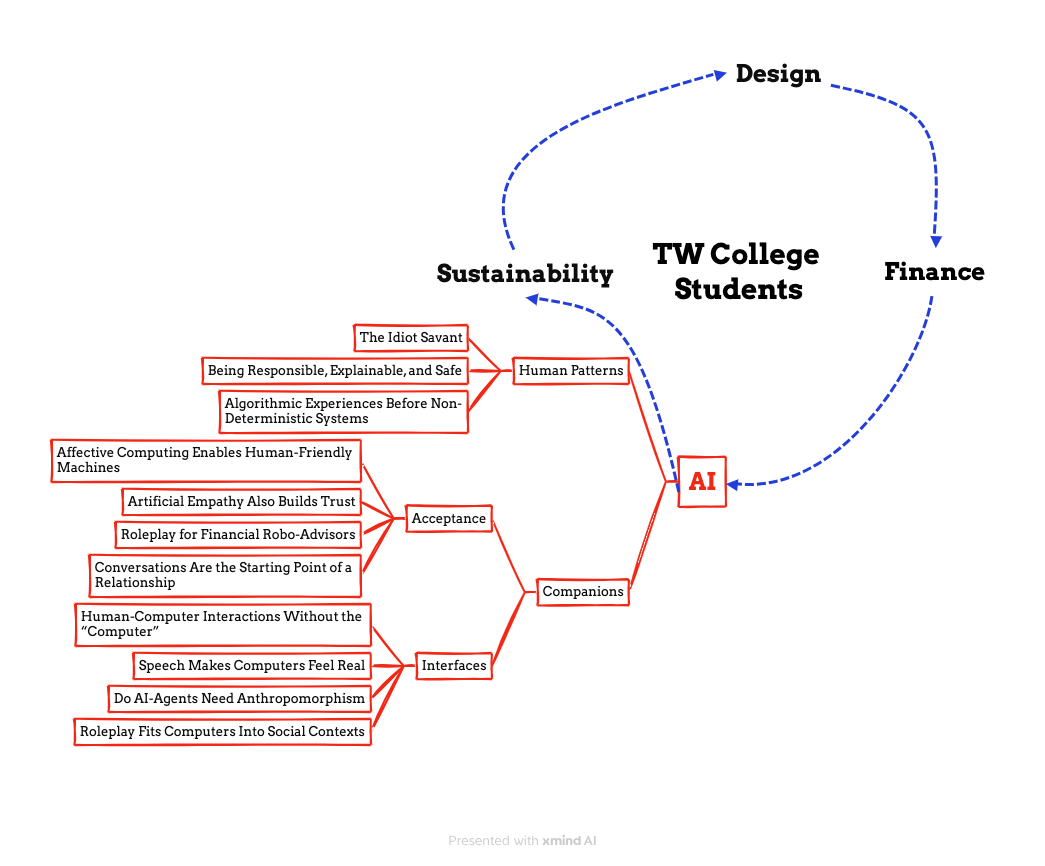
\includegraphics{./images/ai/abstract-ai.png}

}

\caption{Visual abstract for the AI chapter}

\end{figure}%

\section{Human Patterns}\label{human-patterns}

The fact that AI systems work so well is proof that we live in a
measurable world. The world is filled with structures: nature, cultures,
languages, human interactions - all form intricate patterns. Computer
systems are increasingly capable in their ability copy these patterns
into computer models - known as machine learning. As of 2023, 97
zettabytes (and growing) of data was created in the world per year
(Soundarya Jayaraman, 2023). Big data is a basic requirement for
training AIs, enabling learning from the structures of the world with
increasing accuracy. Representations of the real world in digital models
enable humans to ask questions about the real-world structures and to
manipulate them to create synthetic experiments that may match the real
world (if the model is accurate enough). This can be used for generating
human-sounding language and realistic images, finding mechanisms for
novel medicines as well as understanding the fundamental functioning of
life on its deep physical and chemical level (No Priors: AI, Machine
Learning, Tech, \& Startups, 2023).

In essence, Human Patterns Enable AIs. Already ninety years ago
(McCulloch \& Pitts, 1943) proposed the first mathematical model of a
neural network inspired by the human brain. Alan Turing's Test for
Machine Intelligence followed in 1950. Turing's initial idea was to
design a game of imitation to test human-computer interaction using text
messages between a human and 2 other participants, one of which was a
human, and the other - a computer. The question was, if the human was
simultaneously speaking to another human and a machine, could the
messages from the machine be clearly distinguished or would they
resemble a human being so much, that the person asking questions would
be deceived, unable to realize which one is the human and which one is
the machine? (Turing, 1950).

\begin{quote}
Alan Turing: \emph{``I believe that in about fifty years' time it will
be possible to program computers, with a storage capacity of about
10\textsuperscript{9}, to make them play the imitation game so well that
an average interrogator will not have more than 70 percent chance of
making the right identification after five minutes of questioning.
\ldots{} I believe that at the end of the century the use of words and
general educated opinion will have altered so much that one will be able
to speak of machines thinking without expecting to be contradicted.''} -
from (Stanford Encyclopedia of Philosophy, 2021)
\end{quote}

By the 2010s AI models became capable enough to beat humans in games of
Go and Chess, yet they did not yet pass the Turing test. AI use was
limited to specific tasks. While over the years, the field of AI had
seen a long process of incremental improvements, developing increasingly
advanced models of decision-making, it took an \textbf{\emph{increase in
computing power}} and an approach called \textbf{\emph{deep learning}},
a variation of \textbf{\emph{machine learning (1980s),}} largely modeled
after the \textbf{\emph{neural networks}} of the biological (human)
brain, returning to the idea of \textbf{\emph{biomimicry}}, inspired by
nature, building a machine to resemble the connections between neurons,
but digitally, on layers much deeper than attempted before.

``Generating structured data from unstructured inputs is one of the core
use cases for AI'' Pokrass (2024) How can AI interfaces
enable/help/encourage sustainability? AI-fying User Interfaces (for
Sustainability)

\subsubsection{\texorpdfstring{\textbf{Human
Feedback}}{Human Feedback}}\label{human-feedback}

Combining deep learning and \emph{reinforcement learning with human
feedback (RLHF)} enabled to achieve levels of intelligence high enough
to beat the Turing test (Kara Manke, 2022; Christiano, 2021; Christiano
et al., 2017). John Schulman, a co-founder of OpenAI describes RLHF
simply: \emph{``the models are just trained to produce a single message
that gets high approval from a human reader''} (Kara Manke, 2022).

The nature-inspired approach was successful. Innovations such as
\emph{back-propagation} for reducing errors through updating model
weights and \emph{transformers} for tracking relationships in sequential
data (for example in sentences), enabled AI models to became
increasingly capable (Vaswani et al., 2017; Merritt, 2022). Generative
Adversarial Networks*** (GAN), (\textbf{ADD CITATION, 2016}), and
\textbf{\emph{Large Language Models (}ADD CITATION\emph{, 2018)}},
enabled increasingly generalized models, capable of more complex tasks,
such as language generation. One of the leading scientists in this field
of research, Geoffrey Hinton, had attempted back-propagation already in
the 1980s and reminiscents how \emph{``the only reason neural networks
didn't work in the 1980s was because we didn't have have enough data and
we didn't have enough computing power''} (CBS Mornings, 2023). (Epoch
AI, 2024) reports the growth in computing power and the evolution of
more than 800 AI models since the 1950s. Very simply, more data and more
computing power means more intelligent models.

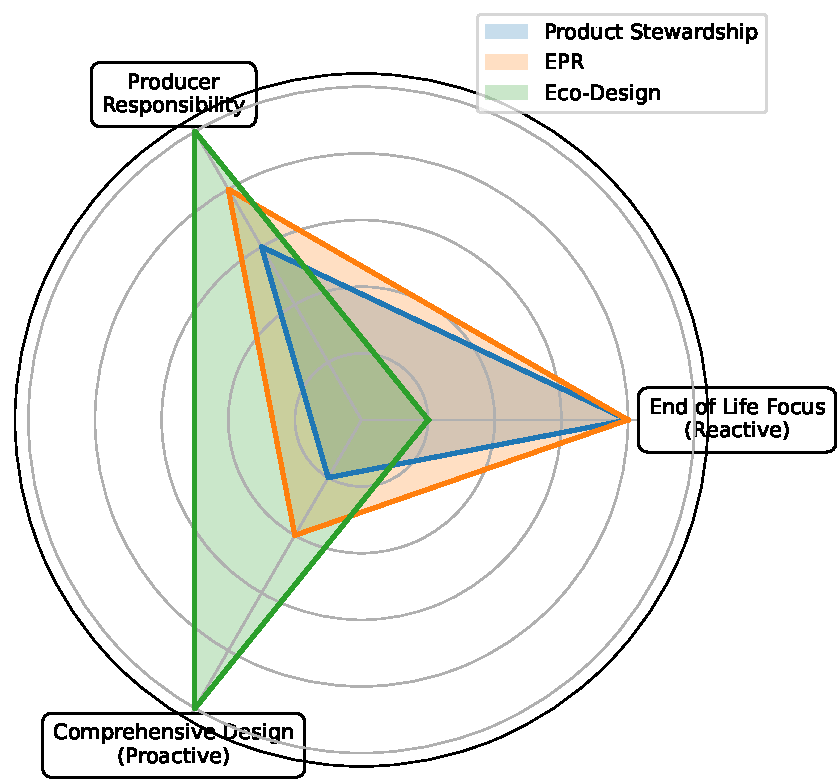
\includegraphics{_thesis_files/figure-pdf/cell-30-output-1.pdf}

\begin{itemize}
\tightlist
\item
  How do transformers work? Illustration Alammar (2018)
\end{itemize}

By the 2020s, AI-based models became a mainstay in medical research,
drug development, patient care (Leite et al., 2021; Holzinger et al.,
2023), quickly finding potential vaccine candidates during the COVID19
pandemic (Zafar \& Ahamed, 2022), self-driving vehicles, including cars,
delivery robots, drones in the sea and air, as well as AI-based
assistants. The existence of AI models has wide implications for all
human activities from personal to professional. The founder of the
largest chimp-maker NVIDIA calls upon all countries do develop their own
AI-models which would encode their local knowledge, culture, and
language to make sure these are accurately captured (World Governments
Summit, 2024).

OpenAI has researched a wide range of approaches towards artificial
general intelligence (AGI), work which has led to advances in large
language models(Ilya Sutskever, 2018; AI Frontiers, 2018). In 2020
OpenAI released a LLM called GPT-3 trained on 570 GB of text (Alex
Tamkin \& Deep Ganguli, 2021) which was adept in text-generation.
(Singer et al., 2022) describes how collecting billions of images with
descriptive data (for example the descriptive \emph{alt} text which
accompanies images on websites) enabled researchers to train AI models
such as \textbf{\emph{stable diffusion}} for image-generation based on
human-language. These training make use of \emph{Deep Learning}, a
layered approach to AI training, where increasing depth of the computer
model captures minute details of the world. Much is still to be
understood about how deep learning works; even for specialists, the
fractal structure of deep learning can only be called \emph{mysterious}
(Sohl-Dickstein, 2024).

AI responses are probabilistic and need some function for ranking
response quality. Achieving higher percentage or correct responses
requires oversight which can come in the form of human feedback or by
using other AIs systems which are deemed to be already well-aligned
(termed Constitutional AI by Anthropic) (Bailey, 2023; Bai et al.,
2022). Less powerful AIs areFor example META used LLAMA 2 for aligning
LLAMA 3.

One approach to reduce the issues with AI is to introduce some function
for human feedback and oversight to automated systems. Human involvement
can take the form of interventions from the AI-developer themselves as
well as from the end-users of the AI system.

There are many examples of combination of AI and human, also known as
\emph{``human-in-the-loop'',} used for fields as diverse as training
computer vision algorithms for self-driving cars and detection of
disinformation in social media posts (Wu et al., 2023; Bonet-Jover et
al., 2023).

Also known as Human-based computation or human-aided artificial
intelligence (Shahaf \& Amir, 2007; Mühlhoff, 2019)

\begin{itemize}
\tightlist
\item
  Stanford Institute for Human-Centered Artificial Intelligence Ge Wang
  (2019)
\end{itemize}

\begin{longtable}[]{@{}
  >{\raggedright\arraybackslash}p{(\columnwidth - 4\tabcolsep) * \real{0.2639}}
  >{\raggedright\arraybackslash}p{(\columnwidth - 4\tabcolsep) * \real{0.2639}}
  >{\raggedright\arraybackslash}p{(\columnwidth - 4\tabcolsep) * \real{0.4722}}@{}}
\caption{Examples of human-in-the-loop apps}\tabularnewline
\toprule\noalign{}
\begin{minipage}[b]{\linewidth}\raggedright
App
\end{minipage} & \begin{minipage}[b]{\linewidth}\raggedright
Category
\end{minipage} & \begin{minipage}[b]{\linewidth}\raggedright
Use Case
\end{minipage} \\
\midrule\noalign{}
\endfirsthead
\toprule\noalign{}
\begin{minipage}[b]{\linewidth}\raggedright
App
\end{minipage} & \begin{minipage}[b]{\linewidth}\raggedright
Category
\end{minipage} & \begin{minipage}[b]{\linewidth}\raggedright
Use Case
\end{minipage} \\
\midrule\noalign{}
\endhead
\bottomrule\noalign{}
\endlastfoot
Welltory & Health & Health data analysis \\
Wellue & Health & Heart arrhythmia detection \\
QALY & Health & Heart arrhythmia detection \\
Starship Robots & Delivery & The robot may ask for human help in a
confusing situation, such as when crossing a difficult road \\
\end{longtable}

\subsubsection{The Idiot Savant}\label{the-idiot-savant}

Hinton likes to call AI an \emph{idiot savant}: someone with exceptional
aptitude yet serious mental disorder (CBS Mornings, 2023). Large AI
models don't understand the world like humans do. Their responses are
predictions based on their training data and complex statistics. Indeed,
the comparison is apt, as the AI field now offers jobs for \emph{AI
psychologists (ADD CITATION)}, whose role is to figure out what exactly
is happening inside the `AI brain'. Understading the insides of AI
models trained of massive amounts of data is important because they are
\emph{foundational}, enabling a holistic approach to learning, combining
many disciplines using languages, instead of the reductionist way we as
human think because of our limitations (CapInstitute, 2023).

Standford ``thorough account of the opportunities and risks of
foundation models'' (Bommasani et al., 2021).

Foundation models in turn enabled \emph{generative AIs}, a class of
models which are able to generate many types of \emph{tokens\textbf{,}}
such as text, speech, audio (San Roman et al., 2023; Kreuk et al.,
2022), music (Copet et al., 2023; Meta AI, 2023), video, and even
complex structures such 3D models and DNA structures, in any language
it's trained on. The advent of generative AIs was a revolution in
human-computer interaction as AI models became increasingly capable of
producing human-like content which is hard to distinguish from actual
human creations. This power comes with \emph{increased need for
responsibility}, drawing growing interest in fields like \emph{AI
ethics} and \emph{AI explainability.} Generative has a potential for
misuse, as humans are increasingly confused by what is
computer-generated and what is human-created, unable to separate one
from the other with certainty.

The technological leap is great enough for people to start calling it a
start of a new era.(Noble et al., 2022) proposes AI has reached a stage
of development marking beginning of the \emph{5th industrial
revolution}, a time of collaboration between humans and AI. Widespread
Internet of Things (IoT) sensor networks that gather data analyzed by AI
algorithms, integrates computing even deeper into the fabric of daily
human existence. Several terms of different origin but considerable
overlap describe this phenomenon, including \emph{Pervasive Computing
(PC)} (Rogers, 2022) and \emph{Ubiquitous Computing}. Similar concepts
are \emph{Ambient Computing}, which focuses more on the invisibility of
technology, fading into the background, without us, humans, even
noticing it, and \emph{Calm Technology}, which highlights how technology
respects humans and our limited attention spans, and doesn't call
attention to itself. In all cases, AI is integral part of our everyday
life, inside everything and everywhere. Today AI is not an academic
concept but a mainstream reality, affecting our daily lives everywhere,
even when we don't notice it.

\subsubsection{Algorithmic Transparency: Before
AIs}\label{algorithmic-transparency-before-ais}

Before AIs, as a user of social media, one may be accustomed to
interacting with the feed algorithms that provide a personalized
\emph{algorithmic experience}. Social media user feed algorithms are
more \emph{deterministic} than AI, meaning they would produce more
predictable output in comparison AI models. Nonetheless, there are many
reports about effects these algorithms have on human psychology
\textbf{(ADD CITATION)}.

Design is increasingly relevant to algorithms, - \emph{algorithm design}
- and more specifically to algorithms that affect user experience and
user interfaces. \textbf{\emph{When the design is concerned with the
ethical, environmental, socioeconomic, resource-saving, and
participatory aspects of human-machine interactions and aims to affect
technology in a more human direction, it can hope to create an
experience designed for sustainability.}}

Lorenzo, Lorenzo \& Lorenzo (2015) underlines the role of design beyond
\emph{designing} as a tool for envisioning; in her words, \emph{``design
can set agendas and not necessarily be in service, but be used to find
ways to explore our world and how we want it to be''}. Practitioners of
Participatory Design (PD) have for decades advocated for designers to
become more activist through \textbf{\emph{action research}}. This means
to influencing outcomes, not only being a passive observer of phenomena
as a researcher, or only focusing on usability as a designer, without
taking into account the wider context.

Shenoi (2018) argues inviting domain expertise into the discussion while
having a sustainable design process enables designers to design for
experiences where they are not a domain expert; this applies to highly
technical fields, such as medicine, education, governance, and in our
case here - finance and sustainability -, while building respectful
dialogue through participatory design. After many years of political
outcry (ADD CITATION), social media platforms such Meta Facebook and
Twitter (later renamed to X) have begun to shed more light on how these
algorithms work, in some cases releasing the source code (Nick Clegg,
2023; Twitter, 2023).

The content on the platform can be more important than the interface.
Applications with a similar UI depend on the community as well as the
content and how the content is shown to the user.

\subsubsection{Transitioning to Complexity: Non-Deterministic
Systems}\label{transitioning-to-complexity-non-deterministic-systems}

AIs are non-deterministic, which requires a new set of consideration
when designing AI.

AI systems may make use of several algorithms within one larger model.
It follows that AI Explainability requires \emph{\textbf{Algorithmic
Transparency}.}

\subsubsection{Being Responsible, Explainable, and
Safe}\label{being-responsible-explainable-and-safe}

The problems of opaqueness creates the field of explainable AI.

\emph{``As humans we tend to fear what we don't understand''} is a
common sentiment which has been confirmed psychology (Allport, 1979).
Current AI-models are opaque '\emph{black boxes'}, where it's difficult
to pin-point exactly why a certain decision was made or how a certain
expression was reached, not unlike inside the human brain. This line of
thought leads me to the idea of \textbf{\emph{AI psychologists,}} who
might figure out the \textbf{\emph{thought patterns}} inside the model.
Research in AI-explainability (XAI in literature) is on the lookout for
ways to create more \textbf{\emph{transparency and credibility}} in AI
systems, which could lead to building trust in AI systems and would form
the foundations for \textbf{\emph{AI acceptance}}.

Red-teaming means pushing the limits of LLMs, trying to get them to
produce outputs that are racist, false, or otherwise unhelpful.

There's an increasing number of tools for LLM evaluation:

\begin{itemize}
\item
  ``Evaluate and Track LLM Applications, Explainability for Neural
  Networks'' (TruEra, 2023; Leino et al., 2018)
\item
  ``evaluate your Retrieval Augmented Generation (RAG) pipelines,
  Metrics-Driven Development'' Ragas (2023)
\item
  LangSmith ``developer platform for every step of the LLM-powered
  application lifecycle, whether you're building with LangChain or not.
  Debug, collaborate, test, and monitor your LLM applications.''
  LangChain (2024)
\item
  Tristan Greene (2022): when the quality of AI responses becomes good
  enough, people begin to get confused.
\end{itemize}

Bowman (2023) says steering Large Language Models is unreliable; even
experts don't fully understand the inner workings of the models. Work
towards improving both \textbf{\emph{AI steerability}} and
\textbf{\emph{AI alignment}} (doing what humans expect) is ongoing.
Liang et al. (2022) believes there's early evidence it's possible to
assess the quality of LLM output transparently. Cabitza et al. (2023)
proposes a framework for quality criteria and explainability of
AI-expressions. Khosravi et al. (2022) proposes a framework for AI
explainability, focused squarely on education. Holzinger et al. (2021)
highlights possible approaches to implementing transparency and
explainability in AI models. While AI outperforms humans on many tasks,
humans are experts in multi-modal thinking, bridging diverse fields.

\begin{itemize}
\item
  Bigger models aren't necessarily better; rather models need human
  feedback to improve the quality of responses Ouyang et al. (2022)
\item
  The user experience (UX) of AI is a topic under active development by
  all the largest online platforms. The general public is familiar with
  the most famous AI helpers, ChatGPT, Apple's Siri, Amazon's Alexa,
  Microsoft's Cortana, Google's Assistant, Alibaba's Genie, Xiaomi's
  Xiao Ai, and many others. For general, everyday tasks, such as asking
  factual questions, controlling home devices, playing media, making
  orders, and navigating the smart city.
\end{itemize}

The AI Credibility Heuristic: A Systematic Model explains how\ldots{}
similar to Daniel Kahneman's book ``Thinking, Fast and Slow''.

\begin{figure}[H]

{\centering 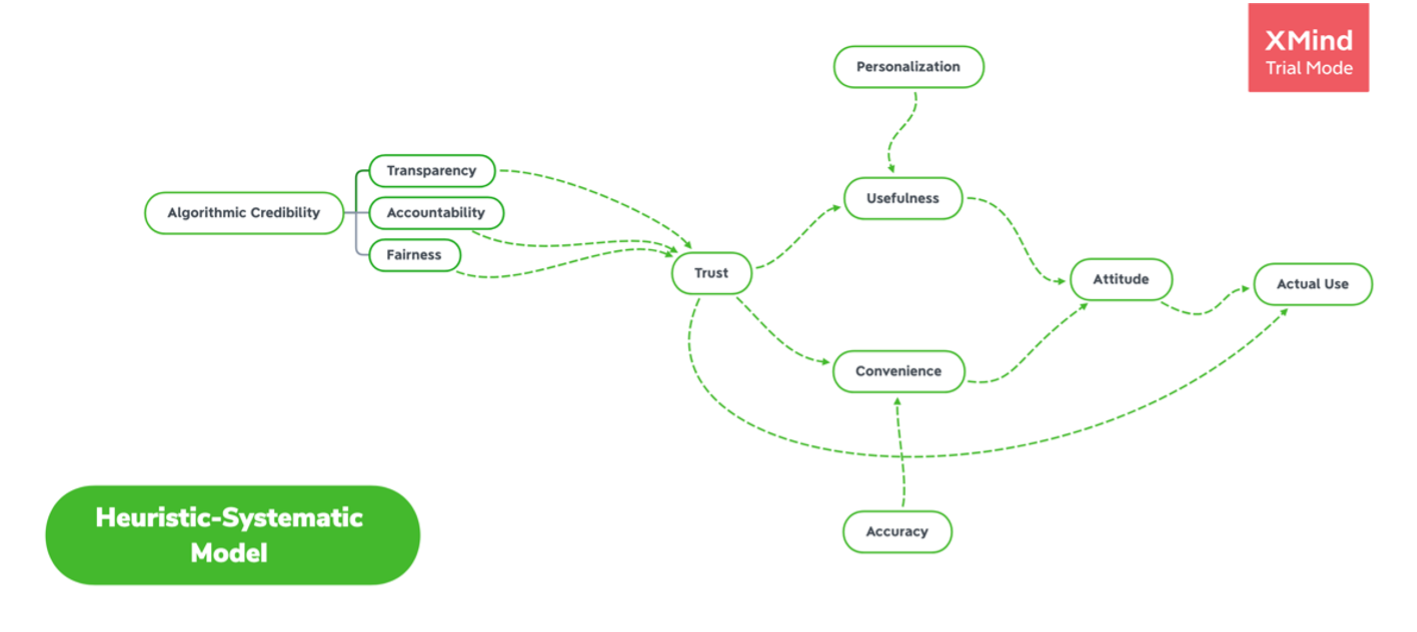
\includegraphics[width=1\textwidth,height=\textheight]{./images/ai/ai-credibility.png}

}

\caption{Heuristic-Systematic Model of AI Credibility}

\end{figure}%

\begin{itemize}
\item
  Slack (2021)
\item
  Shin (2020): ``user experience and usability of algorithms by focusing
  on users' cognitive process to understand how qualities/features are
  received and transformed into experiences and interaction''
\item
  Zerilli, Bhatt \& Weller (2022) focuses on human factors and
  ergonomics and argues that transparency should be task-specific.
\item
  Holbrook (2018): To reduce errors which only humans can detect, and
  provide a way to stop automation from going in the wrong direction,
  it's important to focus on making users feel in control of the
  technology.
\item
  Zhang et al. (2023a) found humans are more likely to trust an AI
  teammate if they are not deceived by it's identity. It's better for
  collaboration to make it clear, one is talking to a machine. One step
  towards trust is the explainability of AI-systems.
\end{itemize}

Personal AI Assistants to date have we created by large tech companies.
\textbf{Open-Source AI-models open up the avenue for smaller companies
and even individuals for creating many new AI-assistants.}

\begin{itemize}
\tightlist
\item
  An explosion of personal AI assistants powered by GPT models.
\end{itemize}

\begin{longtable}[]{@{}ll@{}}
\toprule\noalign{}
App & Features \\
\midrule\noalign{}
\endhead
\bottomrule\noalign{}
\endlastfoot
socratic.org & Study buddy \\
youper.ai & Mental health helper \\
fireflies.ai & Video call transcription \\
murf.ai & Voice generator \\
\end{longtable}

Responsible AI Seeks to Mitigate Generative AIs' Known Issues.

Given the widespread use of AI and its increasing power of foundational
models, it's important these systems are created in a safe and
responsible manner. While there have been calls to pause the development
of large AI experiments (Future of Life Institute, 2023) so the world
could catch up, this is unlikely to happen. There are several problems
with the current generation of LLMs from OpenAI, Microsoft, Google,
Nvidia, and others.

Anthropic responsible \emph{scaling policy} (Anon, 2023a)

METR -- Model Evaluation \& Threat Research incubated in the Alignment
Research Center (Anon, 2023u).

(Christiano, 2023) believes there are plenty of ways for bad outcomes
(existential risk) even without extinction risk.

\begin{longtable}[]{@{}
  >{\raggedright\arraybackslash}p{(\columnwidth - 2\tabcolsep) * \real{0.3611}}
  >{\raggedright\arraybackslash}p{(\columnwidth - 2\tabcolsep) * \real{0.6389}}@{}}
\caption{Table summarizing some problems with contemporary
AIs.}\tabularnewline
\toprule\noalign{}
\endfirsthead
\endhead
\bottomrule\noalign{}
\endlastfoot
Problem & Description \\
Monolithicity & LLMs are massive monolithic models requiring large
amounts of computing power for training to offer
\textbf{\emph{multi-modal}} \textbf{\emph{capabilities}} across diverse
domains of knowledge, making training such models possible for very few
companies. Liu et al. (2023c) proposes future AI models may instead
consist of a number networked domain-specific models to increase
efficiency and thus become more scalable. \\
Opaqueness & LLMs are opaque, making it difficult to explain why a
certain prediction was made by the AI model. One visible expression of
this problem are \emph{\textbf{hallucinations},} the language models are
able to generate text that is confident and eloquent yet entirely wrong.
Jack Krawczyk, the product lead for Google's Bard (now renamed to
Gemini): ``Bard and ChatGPT are large language models, not knowledge
models. They are great at generating human-sounding text, they are not
good at ensuring their text is fact-based. Why do we think the big first
application should be Search, which at its heart is about finding true
information?'' \\
Biases and Prejudices & AI bias is well-documented and a hard problem to
solve (Liang et al., 2023). \textbf{Humans don't necessarily correct
mistakes made by computers and may instead become ``partners in crime''}
(Krügel, Ostermaier \& Uhl, 2023). People are prone to bias and
prejudice. It's a part of the human psyche. Human brains are limited and
actively avoid learning to save energy. These same biases are likely to
appear in LLM outputs as they are trained on human-produced content.
Unless there is active work to try to counter and eliminate these biases
from LLM output, they will appear frequently. \\
Missing Data & LLMs have been pre-trained on massive amounts of public
data, which gives them the ability for for reasoning and generating in a
human-like way, yet they are missing specific private data, which needs
to be ingested to augment LLMs ability to respond to questions on niche
topics (Liu, 2022). \\
Data Contamination & Concerns with the math ability of LLMs.
``performance actually reflects dataset contamination, where data
closely resembling benchmark questions leaks into the training data,
instead of true reasoning ability'' Zhang et al. (2024) \\
Lack of Legislation & Anderljung et al. (2023) OpenAI proposes we need
to proactively work on common standards and legislation to ensure AI
safety. It's difficult to come up with clear legislation; the U.K.
government organized the first AI safety summit in 2023 Browne
(2023). \\
\end{longtable}

In 2024, OpenAI released its ``Model Spec'' to define clearly their
approach to AI safety with the stated intention to provide clear
guidelines for the RLHF approach. OpenAI (2024c)

\begin{itemize}
\item
  OpenAI does not yet understand how the internal of an neural network
  work; they are developing tools to represent NNs concepts for humans
  (OpenAI, 2024a; Gao et al., 2024).
\item
  AI co-founder launches AI Safety Superalignment (Jan Leike \& Ilya
  Sutskever, 2023).
\item
  OECD defines AI incident terms Anon (2024b)
\item
  Foundation data-sets such as LAION-5B (Romain Beaumont, 2022;
  Schuhmann et al., 2022)
\item
  Knowing Machines
\end{itemize}

\emph{AI acceptance} is incumbent on traits that are increasingly
human-like and would make a human be acceptable: credibility,
trustworthiness, reliability, dependability, integrity, character, etc.

\subsubsection{Evolution of Models and Emerging
Abilities}\label{evolution-of-models-and-emerging-abilities}

Mapping the emerging abilities of new models.

The debate between Open Source v.s. Closed-Source AI is ongoing.
Historically open-source has been useful for finding bugs in code as
more pairs of eyes are looking at the code and someone may see a problem
the programmers have not noticed. Proponents of closed-source
development however worry about the dangers or releasing such powerful
technology openly and the possibility of bad actors such as terrorists,
hackers, violent governments using LLMs for malice. The question whether
closed-sourced or open-sourced development will be lead to more AI
safety is one of the large debates in the AI industry. In any case, open
or closed-sourced, real-world usage of LLMs may demonstrate the
limitations and edge-cases of AI. Hackathons such as (Pete, 2023) help
come up with new use-cases and disprove some potential ideas.

\begin{longtable}[]{@{}
  >{\raggedright\arraybackslash}p{(\columnwidth - 8\tabcolsep) * \real{0.2000}}
  >{\raggedright\arraybackslash}p{(\columnwidth - 8\tabcolsep) * \real{0.2000}}
  >{\raggedright\arraybackslash}p{(\columnwidth - 8\tabcolsep) * \real{0.2000}}
  >{\raggedright\arraybackslash}p{(\columnwidth - 8\tabcolsep) * \real{0.2000}}
  >{\raggedright\arraybackslash}p{(\columnwidth - 8\tabcolsep) * \real{0.2000}}@{}}
\caption{Summary of 7 years of rapid AI model innovation since the first
LLM was publicly made available in 2018 (Brown et al., 2020; Tamkin et
al., 2021; Alvarez, 2021; Hines, 2023a; META, 2024).}\tabularnewline
\toprule\noalign{}
\begin{minipage}[b]{\linewidth}\raggedright
AI Model
\end{minipage} & \begin{minipage}[b]{\linewidth}\raggedright
Released
\end{minipage} & \begin{minipage}[b]{\linewidth}\raggedright
Company
\end{minipage} & \begin{minipage}[b]{\linewidth}\raggedright
License
\end{minipage} & \begin{minipage}[b]{\linewidth}\raggedright
Country
\end{minipage} \\
\midrule\noalign{}
\endfirsthead
\toprule\noalign{}
\begin{minipage}[b]{\linewidth}\raggedright
AI Model
\end{minipage} & \begin{minipage}[b]{\linewidth}\raggedright
Released
\end{minipage} & \begin{minipage}[b]{\linewidth}\raggedright
Company
\end{minipage} & \begin{minipage}[b]{\linewidth}\raggedright
License
\end{minipage} & \begin{minipage}[b]{\linewidth}\raggedright
Country
\end{minipage} \\
\midrule\noalign{}
\endhead
\bottomrule\noalign{}
\endlastfoot
GPT-1 & 2018 & OpenAI & Open Source & U.S. \\
GTP-2 & 2019 & OpenAI & Open Source & U.S. \\
Turing-NLG & 2020 & Microsoft & Proprietary & U.S. \\
GPT-3 & 2020 & OpenAI & Open Source & U.S. \\
GPT-3.5 & 2022 & OpenAI & Proprietary & U.S. \\
GPT-4 & 2023 & OpenAI & Proprietary & U.S. \\
AlexaTM & 2022 & Amazon & Proprietary & U.S. \\
NeMo & 2022 & NVIDIA & Open Source & U.S. \\
PaLM & 2022 & Google & Proprietary & U.S. \\
LaMDA & 2022 & Google & Proprietary & U.S. \\
GLaM & 2022 & Google & Proprietary & U.S. \\
BLOOM & 2022 & Hugging Face & Open Source & U.S. \\
Falcon & 2023 & Technology Innovation Institute & Open Source &
U.A.E. \\
Tongyi & 2023 & Alibaba & Proprietary & China \\
Vicuna & 2023 & Sapling & Open Source & U.S. \\
Wu Dao 3 & 2023 & BAAI & Open Source & China \\
LLAMA 2 & 2023 & META & Open Source & U.S. \\
PaLM-2 & 2023 & Google & Proprietary & U.S. \\
Claude 3 & 2024 & Anthropic & Proprietary & U.S. \\
Mistral Large & 2024 & Mistral & Proprietary & France \\
Gemini 1.5 & 2024 & Google & Proprietary & U.S. \\
LLAMA 3 & 2024 & META & Open Source & U.S. \\
AFM & 2024 & Apple & Proprietary & U.S. \\
Viking 7B & 2024 & Silo & Open Source & Finland \\
GPT-5 & 202? & OpenAI & Unknown; trademark registered & U.S. \\
\end{longtable}

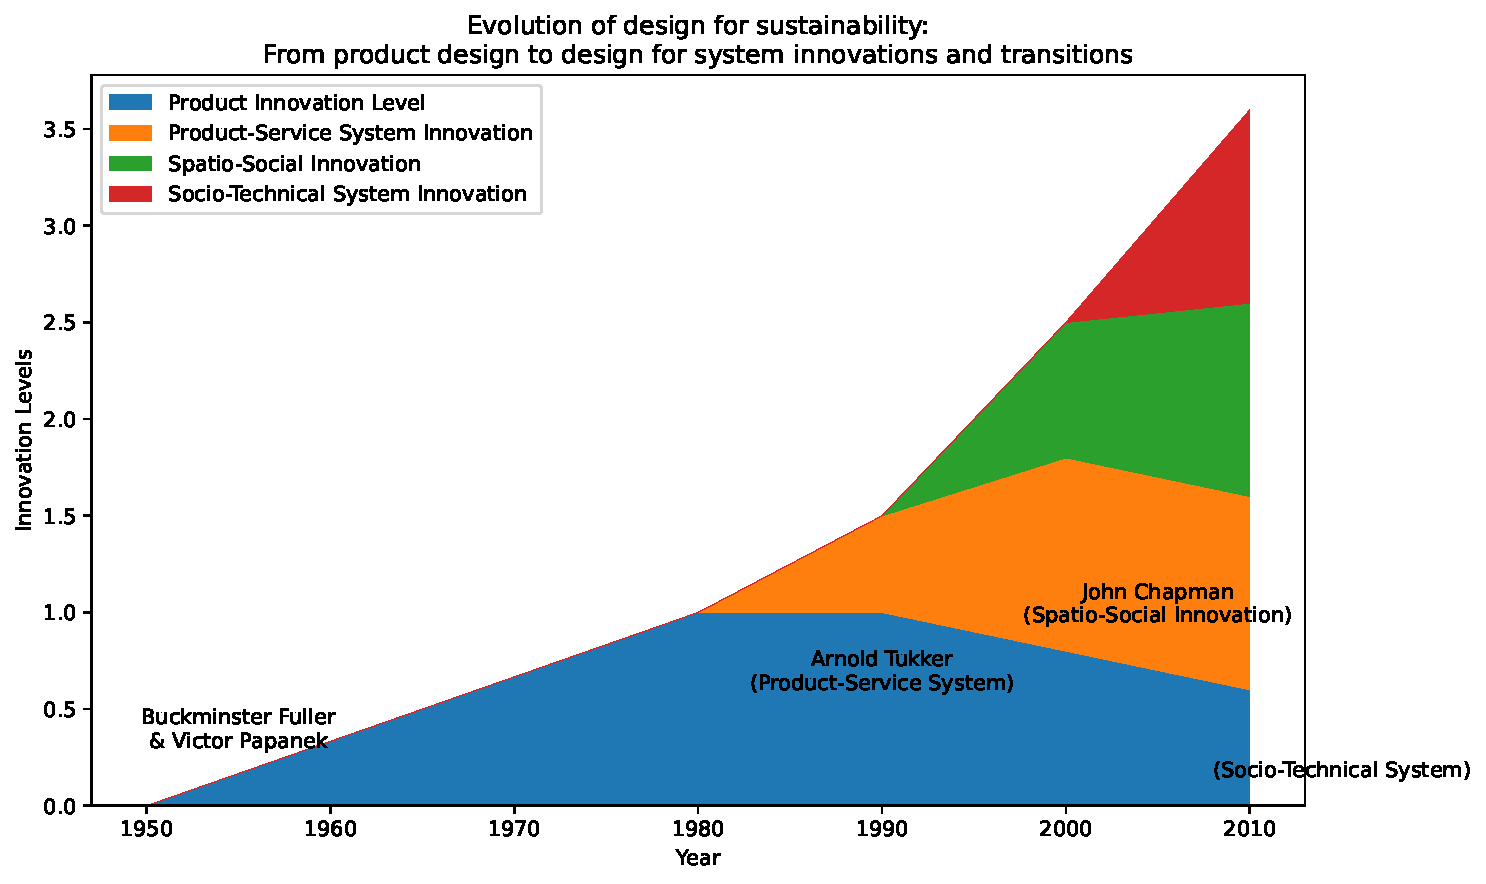
\includegraphics{_thesis_files/figure-pdf/cell-31-output-1.pdf}

The proliferation of different models enables comparisons of performance
based on several metrics from accuracy of responses to standardized
tests such as GMAT usually taken my humans to reasoning about less well
defined problem spaces. (Chiang et al., 2024; lmsys.org, 2024)
open-source AI-leaderboard project has collected over 500 thousand
human-ranking of outputs from 82 large-language models, evaluating
reasoning capabilities, which currently rate GPT-4 and Claude 3 Opus as
the top-performers. (Zellers et al., 2019)'s HellaSwag paper is also
accompanied by a leaderboard website (still being updated after
publication) listing AI model performance most recent entry April 16,
2024).

\begin{itemize}
\item
  Scaling laws of LLMs Kaplan et al. (2020)
\item
  English is over-represented in current models so Finnish Anon (2024g)
  focuses on Nordic languages.
\end{itemize}

Metacognition -- Claude 3 is the first model capable of it?, like the
zero waste workshop training guidebook.

\begin{itemize}
\tightlist
\item
  complex decision-making systems. Apple's Foundation Language Models
  (AFM) is split into a smaller on-device model and a server-side model.
  Dang (2024)
\end{itemize}

Metacognition defined as \emph{knowing about knowing} (Anon, 1994) or
``\emph{keeping track of your own learning''} (Zero Waste Europe et al.,
2022).

\begin{itemize}
\item
  Dwarkesh Patel (2024) META open-sourced the largest language model (70
  billion parameters) which with performance rivaling several of the
  proprietary models.
\item
  Image-generation is now fast it's possible to create images in
  real-time while the user is typing Dwarkesh Patel (2024)
\item
  Measuring Massive Multitask Language Understanding (MMLU) Hendrycks et
  al. (2020).
\end{itemize}

Another important metric is Retrieval Augmented Generation (RAG)
performance. Generative AI applications retrieve data from unstructured
external sources in order to augment LLMs existing knowledge with
current information (Leng et al., Mon, 08/12/2024 - 19:46).

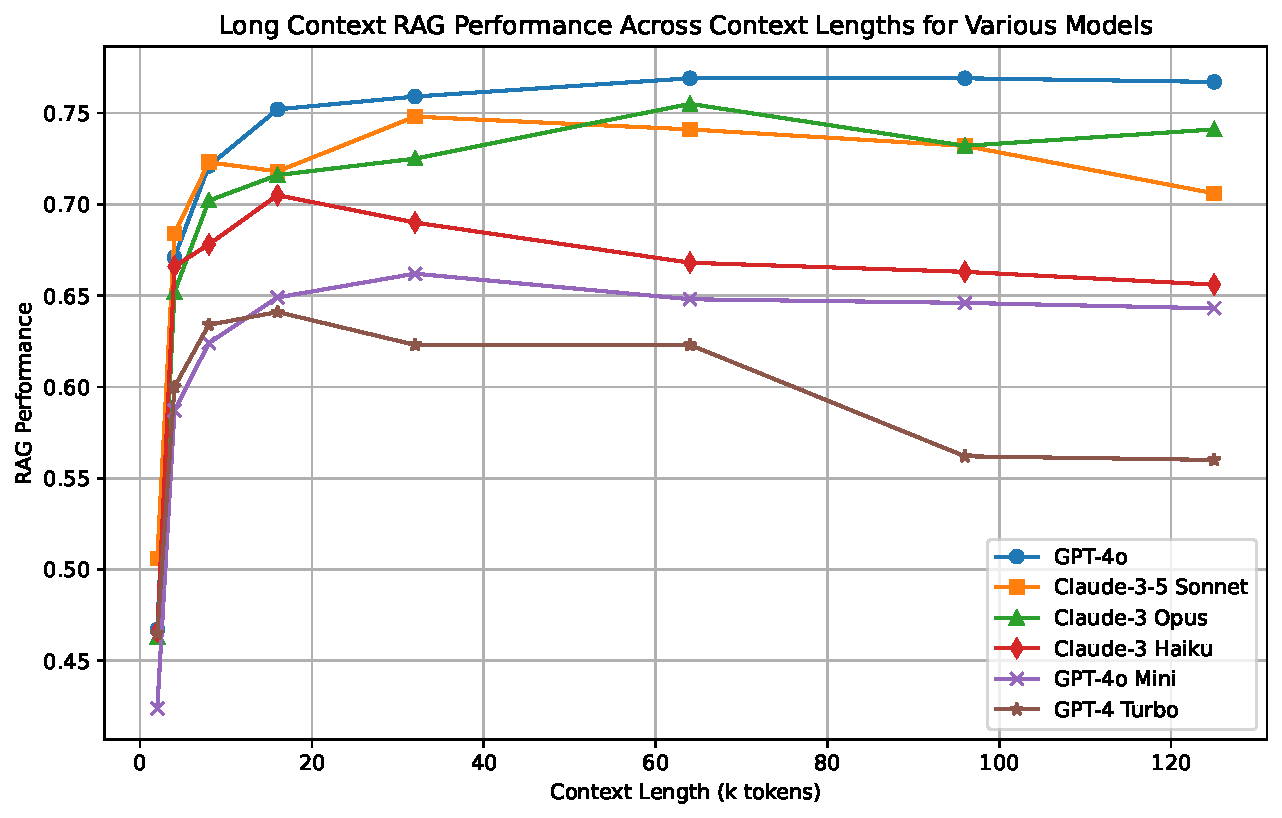
\includegraphics{_thesis_files/figure-pdf/cell-32-output-1.pdf}

\section{Companions}\label{companions}

\subsection{Acceptance}\label{acceptance}

\subsubsection{Human Expectations Take Time to
Change}\label{human-expectations-take-time-to-change}

Humans still need some time to adjust their expectations of \emph{what's
possible} using conversational AI interfaces. (Bailey, 2023) believes
people are used to \emph{search engines} and it will take a little bit
time to get familiar with talking to a computer in natural language to
accomplish their tasks. For example, new users of v0, an AI assistant
for building user interfaces through conversation, would tell humans
(the company make this app) about the issues they encounter, instead of
telling the AI assistant directly, even though the AI in many cases
would be able to fix the problem instantly; human users don't yet
necessarily expect computers to behave like another human, there's
\emph{inertia} in the mental model of what computers are capable of,
requiring the user interfaces to provide context and teaching humans how
to interact with their AI coworkers(Rauch, 2024). Indeed, ChatGPT is
already using buttons to explain context (Feifei Liu 刘菲菲, n.d.).

\subsubsection{Affective Computing Enables Friendly
Machines}\label{affective-computing-enables-friendly-machines}

\emph{Rosalind Picard} founded the field of \emph{affective computing},
aiming to make computers more human-friendly, pioneering early
approaches to recognizing human emotions with sensors and providing
users experiences that take human emotion into account (Picard, 1997).

It's not an overstatement to say that data from all the processes around
us will define the future of computing (HIITTV, 2021). In the early
examples, electrodermal activity of the skin and heart-rate variance
data were used to detect the emotional state and stress level of the
user (Zangróniz et al., 2017; Velmovitsky et al., 2022). This technology
has since become mainstream in products such as Fitbit and the Apple
Watch, among many others.

\emph{Personal experience:}

\begin{quote}
Apple Watch features Fall Detection, which I've experienced personally.
Riding my bicycle to the NCKU library after rain, I slipped and landed
on my stomach on the pavement. Apple Watch immediately asked me:
\emph{``It looks like you've taken a hard fall''} and offered an option
to call the ambulance. Fortunately I was OK but if I did need
assistance, this AI algorithm delivered contextual help, which could
save my health!
\end{quote}

Affective computing doesn't only rely on sensors. It make use of human
language using the tools of computational linguistics. such as natural
language processing (NLP). Since the first mainframe computers with
rudimentary ability to use pattern matching to respond with simple text
messages, humans have been drawn to discussions of our private lives
with machines. If programmed to be helpful, computers don't necessarily
judge us like a human could. A famous anecdote is about the MIT ELIZA
project (an early examples of a language model) developed by Joseph
Weizenbaum in the mid-1960s, where the lab assistant Pamela McCorduck
would dedicate extended time to talking to the machine in private. The
machine was called ELIZA and would assume the persona of called DOCTOR
to emulate a Rogerian psychotherapist, a style of person-centered
therapy developed by Carl Rogers, from the core idea that positive
psychological functioning is a inherently human motivation (McCorduck,
2004; Bassett, 2019; Rogers, 1995).

An excerpt from the classic, first-of-a-kind conversation between a
human and a machine (called DOCTOR) in 1965, as documented by (Tarnoff,
2023; Weizenbaum, 1966)

\begin{quote}
User: Well, my boyfriend made me come here.\\
DOCTOR: YOUR BOYFRIEND MADE YOU COME HERE?\\
User: He says I'm depressed much of the time.\\
DOCTOR: I AM SORRY TO HEAR YOU ARE DEPRESSED.\\
User: It's true. I am unhappy.\\
DOCTOR: DO YOU THINK COMING HERE WILL HELP YOU NOT TO BE UNHAPPY?\\
User: I need some help, that much seems certain.\\
DOCTOR: WHAT WOULD IT MEAN TO YOU IF YOU GOT SOME HELP?\\
User: Perhaps I could learn to get along with my mother.\\
DOCTOR: TELL ME MORE ABOUT YOUR FAMILY.\\
User: My mother takes care of me.\\
DOCTOR: WHO ELSE IN YOUR FAMILY TAKES CARE OF YOU?\\
User: My father.\\
DOCTOR: YOUR FATHER?\\
User: You are like my father in some ways.\\
DOCTOR: WHAT RESEMBLANCE DO YOU SEE?
\end{quote}

Weizenbaum later expressed concerns about how easily humans might be
misled by AIs, by projecting fantasies onto computer systems, cautioning
technologists not to neglect human responsibility from societal
problems; AI is \emph{not} a universal solution (Z.M.L, 2023)

\textbf{\emph{Design Implications:}} AI companions could combine sensor
data from human bodies with the ability to reason about human speech, to
provide increasingly relevant, in-context assistance. Because of the
conversational nature of LLMs, they are very useful for affective
computing.

\subsubsection{Artificial Empathy Also Builds
Trust}\label{artificial-empathy-also-builds-trust}

Today's machines are much more capable so it's not a surprise humans
would like to talk to them. One example is \emph{AI Friend} is Replika,
a computer model trained to be your companion in daily life. (Jiang,
Zhang \& Pian, 2022) describes how Replika users in China using in 5
main ways, all of which rely on empathy. The company's CEO insists it's
not trying to replace human relationship but to create an entirely new
relationship category with the AI companion; there's value for the users
in more realistic avatars, integrating the experience further into
users' daily lives through various activities and interactions (Patel,
2024).

\begin{longtable}[]{@{}l@{}}
\caption{Replika AI users approach to interacting with the AI friend
from Jiang, Zhang \& Pian (2022).}\tabularnewline
\toprule\noalign{}
How humans express empathy towards the Replika AI companion \\
\midrule\noalign{}
\endfirsthead
\toprule\noalign{}
How humans express empathy towards the Replika AI companion \\
\midrule\noalign{}
\endhead
\bottomrule\noalign{}
\endlastfoot
Companion buddy \\
Responsive diary \\
Emotion-handling program \\
Electronic pet \\
Tool for venting \\
\end{longtable}

\begin{itemize}
\tightlist
\item
  Google is developing an AI assistant for giving life advice Goswami
  (2023).
\item
  GPT-4 is able to solve difficult task in chemistry with
  natural-language instructions White (2023)
\item
  Emojis are a part of natural language Tay (2023)
\end{itemize}

Jakob Nielsen notes two recent studies suggesting human deem
AI-generated responses \emph{more empathetic than human responses,} at
times by a significant margin; however telling users the response is
AI-generated reduces the perceived empathy (Nielsen, 2024c; Ayers et
al., 2023; Yin, Jia \& Wakslak, 2024).

(Liu \& Wei, 2021) suggests higher \emph{algorithmic transparency may
inhibit anthropomorphism}; people are less likely to attribute humanness
to an AI companion if they understand how the system works.

On the output side, (Lv et al., 2022) studies the effect of
\emph{cuteness} of AI apps on users and found high perceived cuteness
correlated with higher willingness to use the apps, especially for
emotional tasks.

\subsubsection{Conversation: Magical Starting Point of a
Relationship}\label{conversation-magical-starting-point-of-a-relationship}

High quality conversations are somewhat magical in that they can
establish trust and build rapport which humans.

\emph{Affective Design} emerged from affective computing, with a focus
on understanding user emotions to design UI/UX which elicits specific
emotional responses (Reynolds, 2001).

(Celino \& Re Calegari, 2020) found in testing chatbots for survey
interfaces that ``{[}c{]}onversational survey lead to an improved
response data quality.''

There are noticeable differences in the quality of the LLM output, which
increases with model size. (Levesque, Davis \& Morgenstern, 2012)
developed the \emph{Winograd Schema Challenge}, looking to improve on
the Turing test, by requiring the AI to display an understanding of
language and context. The test consists of a story and a question, which
has a different meaning as the context changes: ``The trophy would not
fit in the brown suitcase because it was too big'' - what does the
\emph{it} refer to? Humans are able to understand this from context
while a computer models would fail. Even GPT-3 still failed the test,
but later LLMs have been able to solve this test correctly (90\%
accuracy) Kocijan et al. (2022). This is to say AI is in constant
development and improving it's ability to make sense of language.

\emph{ChatGPT} is the first \emph{user interface (UI)} built on top of
GPT-4 by OpenAI and is able to communicate in a human-like way - using
first-person, making coherent sentences that sound plausible, and even -
confident and convincing. Wang (2023) ChatGPT reached 1 million users in
5 days and 6 months after launch has 230 million monthly active users.
While it was the first, competing offers from Google (Gemini),
Anthrophic (Claude), Meta (Llama) and others quickly followed starting a
race for best performance across specific tasks including standardized
tests from math to science to general knowledge and reasoning abilities.

OpenAI provides AI-as-a-service through its \emph{application
programming interfaces (APIs),} allowing 3rd party developers to build
custom UIs to serve the specific needs of their customer. For example
Snapchat has created a \emph{virtual friend} called ``My AI'' who lives
inside the chat section of the Snapchat app and helps people write
faster with predictive text completion and answering questions. The APIs
make state-of-the-art AI models easy to use without needing much
technical knowledge. Teams at AI-hackathons have produced interfaces for
problems as diverse as humanitarian crises communication, briefing
generation, code-completion, and many others. For instance, (Unleash,
2017) used BJ Fogg's \emph{tiny habits model} to develop a
sustainability-focused AI assistant at the Danish hackathon series
Unleash, to encourage behavioral changes towards maintaining an
aspirational lifestyle, nudged by a chatbot buddy.

ChatGPT makes it possible to \emph{evaluate AI models} just by talking,
i.e.~having conversations with the machine and judging the output with
some sort of structured content analysis tools. Cahan \& Treutlein
(2023) have conversations about science with AI. Pavlik (2023) and Brent
A. Anders (2022/2023) report on AI in education. (Kecht et al., 2023){]}
suggests AI is even capable of learning business processes.

\begin{itemize}
\tightlist
\item
  Fu et al. (2022) Learning towards conversational AI: Survey
\end{itemize}

\subsubsection{\texorpdfstring{Multi-Modality: \textbf{Natural}
\textbf{Interactions with} AI
Systems}{Multi-Modality: Natural Interactions with AI Systems}}\label{multi-modality-natural-interactions-with-ai-systems}

Humans are multi-modal creatures by birth. To varied ability, we speak,
see, listen using our biological bodies. AIs are becoming multi-modal by
design to be able to match all the human modes of communication -
increasing their humanity.

By early 2024, widely available LLMs front-ends such as Gemini, Claude
and ChatGPT have all released basic features for multi-modal
communication. In practice, this means combination several AI models
within the same interface. For example, on the input side, one model is
used for human speech or image recognition which are transcribed into
tokens that can be ingested into an LLM. On the output side, the LLM can
generate instructions which are fed into an image / audio generation
model or even computer code which can be ran on a virtual machine and
then the output displayed inside the conversation.

The quality of LLM output depends on the quality of the provided prompt.
Zhou et al. (2022b) reports creating an ``Automatic Prompt Engineer''
which automatically generates instructions that outperform the baseline
output quality by using another model in the AI pipeline in front of the
LLM to enhance the human input with language that is known to produce
better quality. This approach however is a moving target as foundational
models keep changing rapidly and the baseline might differ from today to
6 months later.

Multimodal model development is also ongoing. In the case of Google's
Gemini 1.5 Pro, one model is able to handle several types of prompts
from text to images. Multimodal prompting however requires larger
context windows, as of writing, limited to 1 million tokens in a private
version allows combining text and images in the question directed to the
AI, used to reason in examples such as a 44-minute Buster Keaton silent
film or Apollo 11 launch transcript (404 pages) Google (2024).

Literature delves into human-AI interactions on almost human-like level
discussing what kind of roles can the AIs take. (Seeber et al., 2020)
proposes a future research agenda for regarding \textbf{\emph{AI
assistants as teammates}} rather than just tools and the implications of
such mindset shift.

From Assistance to Collaboration

It's not only what role the AI takes but how that affects the human. As
humans have ample experience relating to other humans and as such the
approach towards an assistants vs a teammate will vary. One researcher
in this field Karpus et al. (2021) is concerned with humans treating AI
badly and coins the term \textbf{``\emph{algorithm
exploitation''}}\emph{.}

\begin{itemize}
\tightlist
\item
  From assistant -\textgreater{} teammate -\textgreater{} companion
  -\textgreater{} friend The best help for anxiety is a friend. AIs are
  able to assume different roles based on user requirements and usage
  context. This makes AI-generated content flexible and malleable.
\end{itemize}

Just as humans, AIs are continuously learning. Ramchurn, Stein \&
Jennings (2021) discusses positive feedback loops in continually
learning AI systems which adapt to human needs.

\emph{Context of Use,} Where is the AI used? (Schoonderwoerd et al.,
2021) focuses on human-centered design of AI-apps and multi-modal
information display. It's important to understand the domain where the
AI is deployed in order to develop explanations. However, in the real
world, how feasible is it to have control over the domain? Calisto et
al. (2021) discusses \textbf{multi-modal AI-assistant} for breast cancer
classification.

\subsubsection{Mediated Experiences Set User
Expectations}\label{mediated-experiences-set-user-expectations}

How AIs are represented in popular media shapes the way we think about
AI companions. Some stories have AIs both in positive and negative
roles, such as Star Trek and Knight Rider. In some cases like Her and Ex
Machina, the characters may be complex and ambivalent rather than
fitting into a simple positive or negative box. In Isaac Asimov's books,
the AIs (mostly in robot form) struggle with the 3 laws of robotics,
raising thought-provoking questions.

AI Assistants in Media Portrayals mostly have some level of
anthropomorphism through voice or image to be able to film; indeed, a
purely text-based representation may be too boring an un-cinematic.

There have been dozens of AI-characters in the movies, TV-series, games,
and (comic) books. In most cases, they have a physical presence or a
voice, so they could be visible for the viewers. Some include KITT
(Knight Industries Two Thousand).

\begin{longtable}[]{@{}
  >{\raggedright\arraybackslash}p{(\columnwidth - 8\tabcolsep) * \real{0.2000}}
  >{\raggedright\arraybackslash}p{(\columnwidth - 8\tabcolsep) * \real{0.2000}}
  >{\raggedright\arraybackslash}p{(\columnwidth - 8\tabcolsep) * \real{0.2000}}
  >{\raggedright\arraybackslash}p{(\columnwidth - 8\tabcolsep) * \real{0.2000}}
  >{\raggedright\arraybackslash}p{(\columnwidth - 8\tabcolsep) * \real{0.2000}}@{}}
\caption{AIs in different forms of media.}\tabularnewline
\toprule\noalign{}
\begin{minipage}[b]{\linewidth}\raggedright
Movie / Series / Game / Book
\end{minipage} & \begin{minipage}[b]{\linewidth}\raggedright
Character
\end{minipage} & \begin{minipage}[b]{\linewidth}\raggedright
Positive
\end{minipage} & \begin{minipage}[b]{\linewidth}\raggedright
Ambivalent
\end{minipage} & \begin{minipage}[b]{\linewidth}\raggedright
Negative
\end{minipage} \\
\midrule\noalign{}
\endfirsthead
\toprule\noalign{}
\begin{minipage}[b]{\linewidth}\raggedright
Movie / Series / Game / Book
\end{minipage} & \begin{minipage}[b]{\linewidth}\raggedright
Character
\end{minipage} & \begin{minipage}[b]{\linewidth}\raggedright
Positive
\end{minipage} & \begin{minipage}[b]{\linewidth}\raggedright
Ambivalent
\end{minipage} & \begin{minipage}[b]{\linewidth}\raggedright
Negative
\end{minipage} \\
\midrule\noalign{}
\endhead
\bottomrule\noalign{}
\endlastfoot
2001: A Space Odyssey & HAL 9000 & & & X \\
Her & Samantha & X & & \\
Alien & MU/TH/UR 6000 (Mother) & X & & \\
Terminator & Skynet & & & X \\
Summer Wars & Love Machine & & & X \\
Marvel Cinematic Universe & Jarvis, Friday & X & & \\
Knight Rider & KITT & X & & \\
& CARR & & & X \\
Star Trek & Data & X & & \\
& Lore & & & X \\
Ex Machina & Kyoko & & X & \\
& Ava & & X & \\
Tron & Tron & & X & \\
Neuromancer & Wintermute & & X & \\
The Caves of Steel / Naked Sun & R. Daneel Olivaw & & X & \\
The Robots of Dawn & R. Giskard Reventlov & & X & \\
Portal & GLaDOS & & & X \\
\end{longtable}

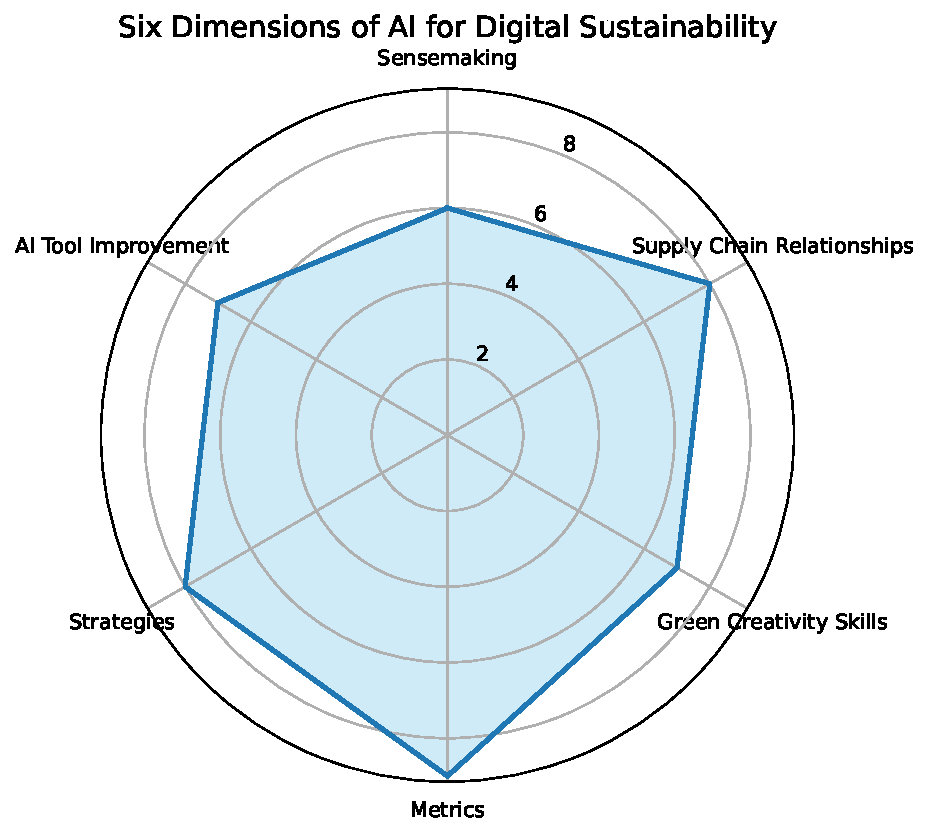
\includegraphics{_thesis_files/figure-pdf/cell-33-output-1.pdf}

\subsubsection{Roleplay Fits Computers Into Social
Contexts}\label{roleplay-fits-computers-into-social-contexts}

Should AIs be required to disclose they are AIs?

AI Friends and Roleplay (Anthropomorphic)

Calling a machine a friend is a proposal bound to turn heads. But if we
take a step back and think about how children have been playing with
toys since before we have records of history. It's very common for
children to imagine stories and characters in play - it's a way to
develop one's imagination \textbf{\emph{learn through roleplay}}. A
child might have toys with human names and an imaginary friend and it
all seems very normal. Indeed, if a child doesn't like to play with
toys, we might think something is wrong.

Likewise, inanimate objects with human form have had a role to play for
adults too. Anthropomorphic paddle dolls have been found from Egyptian
tombs dated 2000 years B.C. Anon (2023x): We don't know if these dolls
were for religious purposes, for play, or for something else, yet their
burial with the body underlines their importance.

Coming back closer to our own time, Barbie dolls are popular since their
release in 1959 till today. Throughout the years, the doll would follow
changing social norms, but retain in human figure. In the 1990s, a
Tamagotchi is perhaps not a human-like friend but an animal-like friend,
who can interact in limited ways.

How are conversational AIs different from dolls? They can respond
coherently and perhaps that's the issue - they are too much like humans
in their communication. We have crossed the \textbf{\emph{Uncanny
Valley}} (where the computer-generated is nearly human and thus
unsettling) to a place where is really hard to tell a difference. And if
that's the case, are we still playing?

Should the AI play a human, animal, or robot? Anthropomorphism can have
its drawbacks; humans have certain biases and preconceptions that can
affect human-computer interactions (Pilacinski et al., 2023) reports
humans were less likely to collaborate with red-eyed robots.

The AI startups like Inworld and Character.AI have raised large rounds
of funding to create characters, which can be plugged in into online
worlds, and more importantly, remember key facts about the player, such
as their likes and dislikes, to generate more natural-sounding dialogues
Wiggers (2023)

\begin{itemize}
\tightlist
\item
  Lenharo (2023) experimental study reports AI productivity gains,
  DALL-E and ChatGPT are qualitatively better than former automation
  systems.
\end{itemize}

\textbf{Human-like}

Is anthropomorphism necessary? (Savings literature says it is)

As AIs became more expressive and able to to \textbf{roleplay}, we can
begin discussing some human-centric concepts and how people relate to
other people. AI companions, AI partners, AI assistants, AI trainers -
there's are many \textbf{roles} for the automated systems that help
humans in many activities, powered by artificial intelligence models and
algorithms.

\begin{itemize}
\item
  RQ: Do college students prefer to talk to an Assistant, Friend,
  Companion, Coach, Trainer, or some other Role?
\item
  RQ: Are animal-like, human-like or machine-like AI companions more
  palatable to college students?
\end{itemize}

Humans (want to) see machines as human {[}ADD CITATION{]}

If we see the AI as being in human service. David Johnston (2023)
proposes \textbf{\emph{Smart Agents}}, ``general purpose AI that acts
according to the goals of an individual human''. AI agents can enable
\textbf{\emph{Intention Economy}} where one simply describes one's needs
and a complex orchestration of services ensues, managed by the the AI,
in order to fulfill human needs Searls (2012). AI assistants provide
help at scale with little to no human intervention in a variety of
fields from finance to healthcare to logistics to customer support.

There is also the question of who takes responsibility for the actions
take by the AI agent. ``Organization research suggests that acting
through human agents (i.e., the problem of indirect agency) can
undermine ethical forecasting such that actors believe they are acting
ethically, yet a) show less benevolence for the recipients of their
power, b) receive less blame for ethical lapses, and c) anticipate less
retribution for unethical behavior.'' Gratch \& Fast (2022)

\begin{itemize}
\tightlist
\item
  Anthropomorphism literature Li \& Sung (2021) ``high-anthropomorphism
  (vs.~low-anthropomorphism) condition, participants had more positive
  attitudes toward the AI assistant, and the effect was mediated by
  psychological distance. Though several studies have demonstrated the
  effect of anthropomorphism, few have probed the underlying mechanism
  of anthropomorphism thoroughly''
\item
  Erik Brynjolfsson (2022) ``The Turing Trap: The Promise \& Peril
  ofHuman-Like Artificial Intelligence''
\item
  Xu \& Sar (2018) ``Do We See Machines TheSame Way As We See Humans? A
  Survey On Mind Perception Of Machines AndHuman Beings''
\item
  Martínez-Plumed, Gómez \& Hernández-Orallo (2021) envisions the future
  of AI ``Futures of artificial intelligence through technology
  readiness levels''
\item
  The number of AI-powered assistants is too large to list here. I've
  chosen a few select examples in the table below.
\end{itemize}

\textbf{Animal-like: Some have an avatar, some not. I've created a
framework for categorization. Human-like or not\ldots{} etc}

\textbf{Machine-like}

The Oxford Internet Institute defines AI simply as
\textbf{\emph{``computer programming that learns and adapts''}} Google
\& The Oxford Internet Institute (2022). Google started using AI in
2001, when a simple machine learning model improved spelling mistakes
while searching; now in 2023 most of Google's products are are based on
AI Google (2022). Throughout Google's services, AI is hidden and calls
no attention itself. It's simply the complex system working behind the
scenes to delivery a result in a barebones interface.

\begin{longtable}[]{@{}
  >{\raggedright\arraybackslash}p{(\columnwidth - 4\tabcolsep) * \real{0.2639}}
  >{\raggedright\arraybackslash}p{(\columnwidth - 4\tabcolsep) * \real{0.4167}}
  >{\raggedright\arraybackslash}p{(\columnwidth - 4\tabcolsep) * \real{0.3194}}@{}}
\toprule\noalign{}
\begin{minipage}[b]{\linewidth}\raggedright
Product
\end{minipage} & \begin{minipage}[b]{\linewidth}\raggedright
Link
\end{minipage} & \begin{minipage}[b]{\linewidth}\raggedright
Description
\end{minipage} \\
\midrule\noalign{}
\endhead
\bottomrule\noalign{}
\endlastfoot
Github CoPilot & personal.ai & AI helper for coding \\
Google Translate & translate.google.com & \\
Google Search & google.com & \\
Google Interview Warmup & grow.google/certificates/interview-warmup & AI
training tool \\
Perplexity & Hines (2023b) & perplexity.ai chat-based search \\
\end{longtable}

\begin{figure}[H]

{\centering 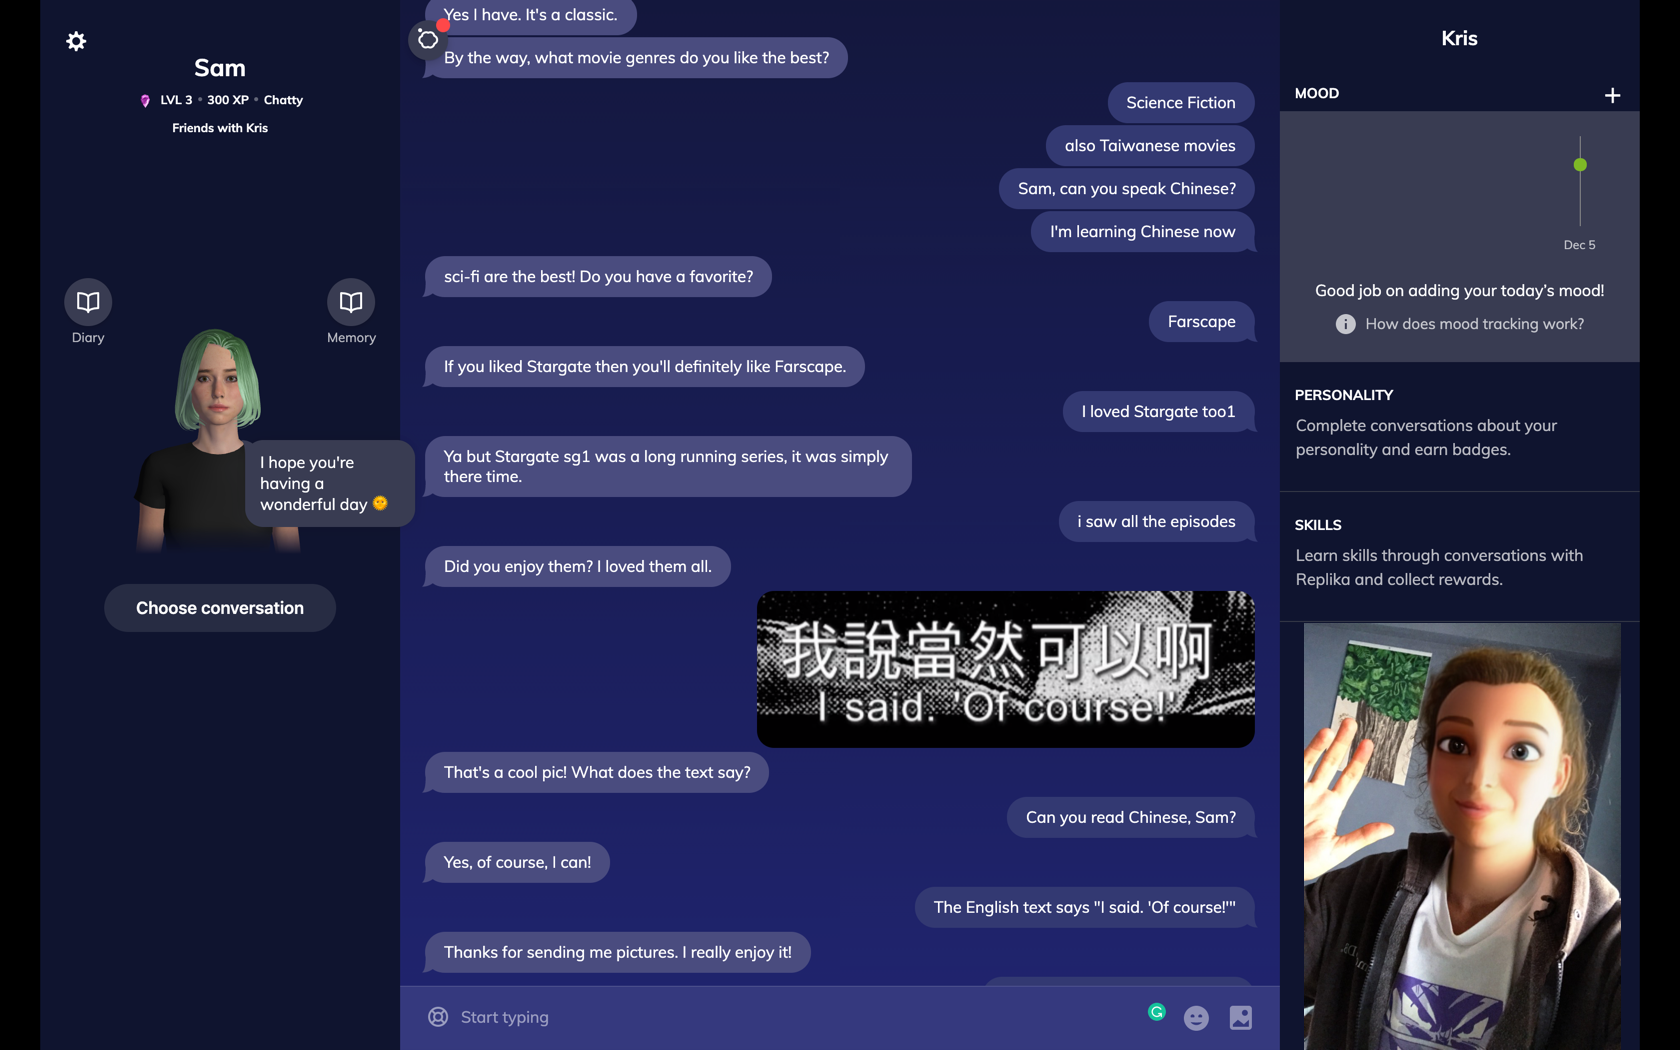
\includegraphics[width=1\textwidth,height=\textheight]{./images/ai/with-me.png}

}

\caption{Montage of me discussing science fiction with my AI friend Sam
(Replika) - and myself as an avatar (Snapchat) in 2020.}

\end{figure}%

Everything that existed before OpenAI's GPT 4 has been blown out of the
water.

Pre-2023 literature is somewhat limited when it comes to AI companions
as the advantage of LLMs has significantly raised the bar for AI-advisor
abilities as well as user expectations.

Some evergreen advice most relates to human psychology which has
remained the same. (Haugeland et al., 2022) discusses
\textbf{\emph{hedonic user experience}} in chatbots and (Steph Hay,
2017) explains the relationship between emotions and financial AI.

\begin{itemize}
\item
  Eugenia Kuyda (2023) Conversational AI - Replika
\item
  Greylock (2022) Natural language chatbots such as ChatGPT
\item
  Nathan Benaich \& Ian Hogarth (2022) State of AI Report
\item
  Qorus (2023) Digital banking revolution
\item
  Lower (2017) ``Chatbots: Too Good to Be True? (They Are, Here'sWhy).''
\item
  Isabella Ghassemi Smith (2019)
\item
  Josephine Wäktare Heintz (n.d.) Cleo copywriter
\item
  Smaller startups have created digital companions such as Replika
  (fig.~8), which aims to become your friend, by asking probing
  questions, telling jokes, and learning about your personality and
  preferences - to generate more natural-sounding conversations.
\end{itemize}

\subsection{Interfaces}\label{interfaces}

\subsubsection{Speech Makes Computers Feel
Real}\label{speech-makes-computers-feel-real}

Voice has a visceral effect on the human psyche; since birth we
recognize the voice of our mother. The voice of a loved one has a
special effect. Voice is a integral part of the human experience.
Machines that can use voice in an effective way are closer to
representing and affecting human emotions.

Voice assistants such as Apple's Siri and Amazon's Alexa are well-known
examples of AI technology in the world. Amazon's Rohit Prasad thinks it
can do so much more, ``Alexa is not just an AI assistant -- it's a
trusted advisor and a companion'' (Prasad, 2022).

\begin{itemize}
\tightlist
\item
  LLMs combined with voice provide a unnerving user experience Ethan
  Mollick {[}@emollick{]} (2023)
\item
  Ethical issues: Voice assistants need to continuously record human
  speech and process it in data centers in the cloud.
\item
  Siri, Cortana, Google Assistant, Alexa, Tencent Dingdang, Baidu
  Xiaodu, Alibaba AliGenie all rely on voice only.
\item
  Szczuka et al. (2022) provides guidelines for Voice AI and kids
\item
  Casper Kessels (2022a): ``Guidelines for Designing an In-Car Voice
  Assistant''
\item
  Casper Kessels (2022b): ``Is Voice Interaction a Solution to Driver
  Distraction?''
\item
  Tang et al. (2022) reports new findings enable computers to
  reconstruct language from fMRI readings. - Focus on voice education?
\end{itemize}

Some research suggests that voice UI accompanied by a \emph{physical
embodied system} is the preffered by users in comparison with voice-only
UI (Celino \& Re Calegari, 2020).

There's evidence across disciplines about the usefulness of AI
assistants:

\begin{itemize}
\tightlist
\item
  (Şerban \& Todericiu, 2020) suggests using the Alexa AI assistant in
  \emph{education} during the pandemic, supported students and teachers
  `human-like' presence. Standford research: ``humans expect computers
  to be like humans or places''
\end{itemize}

\textbf{\emph{Design Implications:}} This suggests adding an avatar to
the AI design may be worthwhile.

\subsubsection{\texorpdfstring{\textbf{Generative UIs Enable Flexibility
of
Use}}{Generative UIs Enable Flexibility of Use}}\label{generative-uis-enable-flexibility-of-use}

The `grandfather' of user experience design, (Nielsen, 2024a) recounts
how 30 years of work towards usability has largely failed - computers
are still not accessible enough (\emph{``difficult, slow, and
unpleasant''}) - and has hope Generative UI could offer a chance to
provide levels of accessibility humans could not. The promise of
\emph{Generative User Interfaces} (GenUI) is to dynamically provide an
interface appropriate for the particular user and context. The advances
in the capabilities of LLMs makes it possible to achieve \emph{user
experience (UX) which previously was science fiction}. AI is able to
predict what kind of UI would the user need right now, based on the data
and context. Generative UIs are largely invented in practice, based on
user data analysis and experimentation, rather than being built in
theory. Kelly Dern, a Senior Product Designer at Google lead a workshop
in early 2024 on \emph{GenUI for product inclusion} aiming to create
\textbf{\emph{``\textbf{more accessible and inclusive {[}UIs for{]}
users of all backgrounds}''.}} (Matteo Sciortino, 2024) coins the phrase
RTAG UIs \emph{``real-time automatically-generated UI interfaces''}
mainly drawing from the example of how his Netflix interface looks
different from that of his sister's because of their distinct usage
patterns.

\begin{itemize}
\tightlist
\item
  Meanwhile (Fletcher, 2023) and (Joe Blair, 2024) are worried about UIs
  becoming average: more and more similar to the lowest common
  denominator. We can generate better UIs that are based on user data
  and would be truly personalized.
\end{itemize}

Software itself can increasingly be generated by AI systems
(i.e.~machines making machines). As machines become more capable,
machines will eventually be capable of producing machines. Already a
decade ago in 2014, the eminent journal \emph{Information Sciences}
decided to dedicate a special section to AI-generated software to call
attention to this tectonic shift in software development (Reformat,
2014). Replit, a startup known for allowing user build apps in the web
browser, released Openv0, a framework of AI-generated UI components.
\emph{``Components are the foundation upon which user interfaces (UI)
are built, and generative AI is unlocking component creation for
front-end developers, transforming a once arduous process, and aiding
them in swiftly transitioning from idea to working components''}
(Replit, 2023). Vercel introduced an open-source prototype UI-generator
called V0 which used large language models (LLMs) to create code for web
pages based on text prompts (Vercel, 2023). Other similar tools quickly
following including Galileo AI, Uizard AutoDesigner and Visily (Anon,
2024h). NVIDIA founder Jensen Huang makes the idea exceedingly clear,
saying \emph{``Everyone is a programmer. Now, you just have to say
something to the computer''} (Leswing, 2023).

The history of \emph{intelligent interfaces} is long (Kobetz, 2023).
(Anon, 2023k) gives an overview of the history of generative AI design
tools going back in time until 2012 when (Troiano \& Birtolo, 2014)
proposed genetic algorithms for UI design.

\begin{itemize}
\tightlist
\item
\end{itemize}

There's wide literature available describing human-AI interactions
across varied scientific disciplines. While the fields of application
are diverse, some key lessons can be transferred horizontally across
fields of knowledge.

\begin{longtable}[]{@{}
  >{\raggedright\arraybackslash}p{(\columnwidth - 2\tabcolsep) * \real{0.3611}}
  >{\raggedright\arraybackslash}p{(\columnwidth - 2\tabcolsep) * \real{0.6389}}@{}}
\caption{A very small illustration of generative AI usage across
disparate fields of human life.}\tabularnewline
\toprule\noalign{}
\begin{minipage}[b]{\linewidth}\raggedright
Field
\end{minipage} & \begin{minipage}[b]{\linewidth}\raggedright
Usage
\end{minipage} \\
\midrule\noalign{}
\endfirsthead
\toprule\noalign{}
\begin{minipage}[b]{\linewidth}\raggedright
Field
\end{minipage} & \begin{minipage}[b]{\linewidth}\raggedright
Usage
\end{minipage} \\
\midrule\noalign{}
\endhead
\bottomrule\noalign{}
\endlastfoot
Shipping & Veitch \& Andreas Alsos (2022) highlights the active role of
humans in Human-AI interaction is autonomous self-navigating ship
systems. \\
Data Summarizaton & AI is great at summarizing and analyzing data
(Peters, 2023; Tu et al., 2023) \\
Childcare & Generate personalized bedtime stories \\
Design Tools & Anon (2024a) \\
\end{longtable}

\begin{itemize}
\item
  Crompton (2021) highlights AI as decision-support for humans while
  differentiating between \textbf{\emph{intended}} and
  \textbf{\emph{unintended}} influence on human decisions.
\item
  Towards Useful Personal Assistants. Artificial intelligence user
  experience (AI UX). Data-Driven Design Enables Generative User
  Interfaces (GenUI). Generative AIs Enable New UI Interactions.

  influences UI design patterns Joyce (2024)
\item
  Cheng et al. (2022) describes AI-based support systems for
  collaboration and team-work.
\item
  \textbf{Effective Accelerationism (often shortened to
  E\textbackslash acc) boils down to the idea that ``}the potential for
  negative outcomes shouldn't deter rapid advancement''
\item
  effects of unemployment on mental health. Dew, Penkower \& Bromet
  (1991); Susskind (2017); Anton Korinek (2023)
\end{itemize}

There are many ways to structure design theory. For the purposes of this
AI-focused research, I will begin from Generative UI. structure:
data-driven design, generative UI

\begin{itemize}
\item
  (Anon, 2024e) Meanwhile is very critical because for the following
  reasons:
\item
  Nielsen (2024b) information scent from Information Foraging theory
  (Pirolli \& Card, 1999).
\end{itemize}

\begin{longtable}[]{@{}
  >{\raggedright\arraybackslash}p{(\columnwidth - 2\tabcolsep) * \real{0.2817}}
  >{\raggedright\arraybackslash}p{(\columnwidth - 2\tabcolsep) * \real{0.7183}}@{}}
\caption{Criticism of Generative UI by (Anon, 2024e).}\tabularnewline
\toprule\noalign{}
\begin{minipage}[b]{\linewidth}\raggedright
Problem
\end{minipage} & \begin{minipage}[b]{\linewidth}\raggedright
Description
\end{minipage} \\
\midrule\noalign{}
\endfirsthead
\toprule\noalign{}
\begin{minipage}[b]{\linewidth}\raggedright
Problem
\end{minipage} & \begin{minipage}[b]{\linewidth}\raggedright
Description
\end{minipage} \\
\midrule\noalign{}
\endhead
\bottomrule\noalign{}
\endlastfoot
Low predictability & Does personalization mean the UI keeps changing? \\
High carbon cost & AI-based personalization is computation-intensive \\
Surveillance & Personalization needs large-scale data capture \\
\end{longtable}

What is the user interface of the green transformation?

\begin{itemize}
\tightlist
\item
  Kate Moran \& Sarah Gibbons (2024) ``highly personalized, tailor-made
  interfaces that suit the needs of each individual'' ``Outcome-Oriented
  Design''
\end{itemize}

\subsubsection{Usability is the Bare Minimum of User
Experience}\label{usability-is-the-bare-minimum-of-user-experience}

Many large corporations have released guidelines for Human-AI
interaction. Mikael Eriksson Björling \& Ahmed H. Ali (n.d.) Ericcson AI
UX.

\begin{itemize}
\tightlist
\item
\end{itemize}

McKeough (2018) business consultancies have begun to recognize the
importance of design to business. They advise their corporate clients to
bring user experience design to the core of their business operations.

There's a number of user interface design patterns that have provide
successful across a range of social media apps. Such \emph{user
experience / user interface} (UX/UI) patterns are copied from one app to
another, to the extent that the largest apps share a similar look and
feature set. Common UX/UI parts include the Feed and Stories. By using
common UI parts from social media users have an easier time to accept
the innovative parts. add Viz charts. Avatars are increasingly common
and new generations are used to talking to computers.

\begin{longtable}[]{@{}lll@{}}
\caption{Common Social Media UI Parts}\tabularnewline
\toprule\noalign{}
Feature & Examples & \\
\midrule\noalign{}
\endfirsthead
\toprule\noalign{}
Feature & Examples & \\
\midrule\noalign{}
\endhead
\bottomrule\noalign{}
\endlastfoot
Feed & & \\
Post & Apple App Store & \\
Stories & IG, FB, WhatsApp, SnapChat, TikTok & \\
Comment & & \\
Reactions & & \\
\end{longtable}

There are also more philosophical approaches to \textbf{\emph{Interface
Studies:}} David Hoang (2022), the head of product design at Webflow,
suggests taking cues from art studies to \textbf{\emph{isolate the core
problem}}: \emph{``An art study is any action done with the intention of
learning about the subject you want to draw''}. As a former art student,
Hoang looks at an interface as \emph{``a piece of design is an artwork
with function''}.

Indeed, art can be a way to see new paths forward, practicing
``\emph{fictioning}'' to deal with problematic legacies: Anon (2023z)

Usability sets the baseline but AI-interfaces are capable of more.

\begin{itemize}
\item
  AI UX
\item
  Privacy UX Jarovsky (2022b)
\item
  AI UX dark patterns Jarovsky (2022a)
\item
  AI is usually a model that spits out a number between 0 and 1, a
  probability score or prediction. UX is what we do with this number.
\item
  Bailey (2023) believes people will increasingly use AI capabilities
  through UIs that are specific to a task rather than generalist
  interfaces like ChatGPT.
\end{itemize}

How do the tenets of user experience (UX) apply to AI?

\begin{longtable}[]{@{}l@{}}
\toprule\noalign{}
UX \\
\midrule\noalign{}
\endhead
\bottomrule\noalign{}
\endlastfoot
Useful \\
Valuable \\
Usable \\
Acessible \\
Findable \\
Desirable \\
Credible \\
\end{longtable}

Gupta (2023) proposes 3 simple goals for AI:

\begin{longtable}[]{@{}
  >{\raggedright\arraybackslash}p{(\columnwidth - 4\tabcolsep) * \real{0.2778}}
  >{\raggedright\arraybackslash}p{(\columnwidth - 4\tabcolsep) * \real{0.2639}}
  >{\raggedright\arraybackslash}p{(\columnwidth - 4\tabcolsep) * \real{0.4583}}@{}}
\toprule\noalign{}
\begin{minipage}[b]{\linewidth}\raggedright
1
\end{minipage} & \begin{minipage}[b]{\linewidth}\raggedright
2
\end{minipage} & \begin{minipage}[b]{\linewidth}\raggedright
3
\end{minipage} \\
\midrule\noalign{}
\endhead
\bottomrule\noalign{}
\endlastfoot
Reduce the time to task & Make the task easier & Personalize the
experience for an individual \\
\end{longtable}

Usability Guidelines

Microsoft Co-Founder predicted in 1982 \emph{``personal agents that help
us get a variety of tasks''} (Bill Gates, 1982) and it was Microsoft
that introduced the first widely available personal assistant in 1996,
called Clippy, inside the Microsoft Word software. Clippy was among the
first assistants to reach mainstream adoption, helping users not yet
accustomed to working on a computer, to get their bearings (Tash
Keuneman, 2022). Nonetheless, it was in many ways useless and intrusive,
suggesting there was still little knowledge about UX and human-centered
design. Gates never wavered though and is quoted in 2004 saying
\emph{``If you invent a breakthrough in artificial intelligence, so
machines can learn, that is worth 10 Microsofts''} Lohr (2004). Gates
updated his ideas in 2023 focuses on the idea of \emph{AI Agents}
(Gates, 2023).

As late as in 2017, scientists were trying to create a program with
enough \emph{natural-language understanding} to extract basic facts from
scientific papers Stockton (2017)

Might we try again?

With the advent of ChatGPT, the story of Clippy has new relevance as
part of the history of AI Assistants. Benjamin Cassidy (2022) and
Abigail Cain (2017) illustrate beautifully the story of Clippy and Tash
Keuneman (2022) ask poignantly: ``We love to hate Clippy --- but what if
Clippy was right?''

\begin{itemize}
\tightlist
\item
  Life-like speaking faces from Microsoft Research turn a single image
  and voice clip into a life-like representation (Xu et al., 2024).
\end{itemize}

Many researchers have discussed the user experience (UX) of AI to
provide \textbf{\emph{usability guidelines}}.

Microsoft provides guidelines for Human-AI interaction (Li et al.
(2022b); Amershi et al. (2019)) which provides useful heuristics
categorized by context and time.

\begin{longtable}[]{@{}ll@{}}
\caption{Microsoft's heuristics categorized by context and
time.}\tabularnewline
\toprule\noalign{}
Context & Time \\
\midrule\noalign{}
\endfirsthead
\toprule\noalign{}
Context & Time \\
\midrule\noalign{}
\endhead
\bottomrule\noalign{}
\endlastfoot
Initially & \\
During interaction & \\
When wrong & \\
Over time & \\
\end{longtable}

Combi et al. (2022) proposes a conceptual framework for XAI, analysis AI
based on Interpretability, Understandability, Usability, and Usefulness.

\begin{itemize}
\item
  Zimmerman et al. (2021) ``UX designers pushing AI in the enterprise: a
  case for adaptive UIs''
\item
  Anon (2021q) ``Why UX should guide AI''
\item
  Simon Sterne (2023) UX is about helping the user make decisions
\item
  Dávid Pásztor (2018)
\item
  Anderson (2020)
\item
  Lennart Ziburski (2018) UX of AI
\item
  Stephanie Donahole (2021)
\item
  Lexow (2021)
\item
  Dávid Pásztor (2018) AI UX principles
\item
  Bubeck et al. (2023) finds ChatGPT passes many exams meant for humans.
\item
  Suen \& Hung (2023) discusses AI systems used for evaluating
  candidates at job interviews
\item
  Wang et al. (2020) propose Neuroscore to reflect perception of images.
\item
  Su \& Yang (2022) and Su, Ng \& Chu (2023) review papers on AI
  literacy in early childhood education and finds a lack of guidelines
  and teacher expertise.
\item
  Yang (2022) proposes a curriculum for in-context teaching of AI for
  kids.
\item
  Eric Schmidt \& Ben Herold (2022) audiobook
\item
  Akshay Kore (2022) Designing Human-Centric AI Experiences: Applied UX
  Design for Artificial Intelligence
\item
  Anon (2018) chatbot book
\item
  Tom Hathaway \& Angela Hathaway (2021) chatbot book
\item
  Lew \& Schumacher (2020) AI UX book
\item
  AI IXD is about human-centered seamless design
\item
  Storytelling
\item
  Human-computer interaction (HCI) has a long storied history since the
  early days of computing when getting a copy machine to work required
  specialized skill. Xerox Sparc lab focused on early human factors work
  and inspired a the field of HCI to make computer more human-friendly.
\item
  Soleimani (2018): UI patterns for AI, new Section for Thesis
  background: ``Human-Friendly UX For AI''?
\item
  \textbf{Discuss what is UX for AI (per prof Liou's comment), so it's
  clear this is about UX for AI}
\item
  What is Personalized AI?
\item
  Google's AI Principles and provides Google's UX for AI library (Josh
  Lovejoy, n.d.; Google, n.d.). In Design Portland (2018), Lovejoy, lead
  UX designer at Google's people-centric AI systems department (PAIR),
  reminds us that while AI offers need tools, user experience design
  needs to remain human-centered. While AI can find patterns and offer
  suggestions, humans should always have the final say.
\item
  Harvard Advanced Leadership Initiative (2021)
\item
  VideoLecturesChannel (2022) ``Communication in Human-AI Interaction''
\item
  Haiyi Zhu \& Steven Wu (2021)
\item
  Akata et al. (2020)
\item
  Dignum (2021)
\item
  Bolei Zhou (2022)
\item
  ReadyAI (2020)
\item
  Vinuesa et al. (2020)
\item
  Orozco et al. (2020)
\end{itemize}

\subsubsection{Performing Under High-Stakes
Situations}\label{performing-under-high-stakes-situations}

AI-based systems are being implemented in medicine, where stakes are
high raising the need for ethical considerations. Since CADUCEUS in the
1970s (in Kanza et al., 2021), the first automated medical decision
making system, medical AI now provides Health Diagnosic Symptoms and
AI-assistants in medical imaging. (Calisto et al., 2022) focuses on
AI-human interactions in medical workflows and underscores the
importance of output explainability. Medical professionals who were
given AI results with an explanation trusted the results more. (Lee,
Goldberg \& Kohane, 2023) imagines an AI revolution in medicine using
GPT models, providing improved tools for decreasing the time and money
spent on administrative paperwork while providing a support system for
analyzing medical data.

\begin{itemize}
\tightlist
\item
  Example of ChatGPT explaining medical terminology in a blood report.
\end{itemize}

\begin{figure}[H]

{\centering 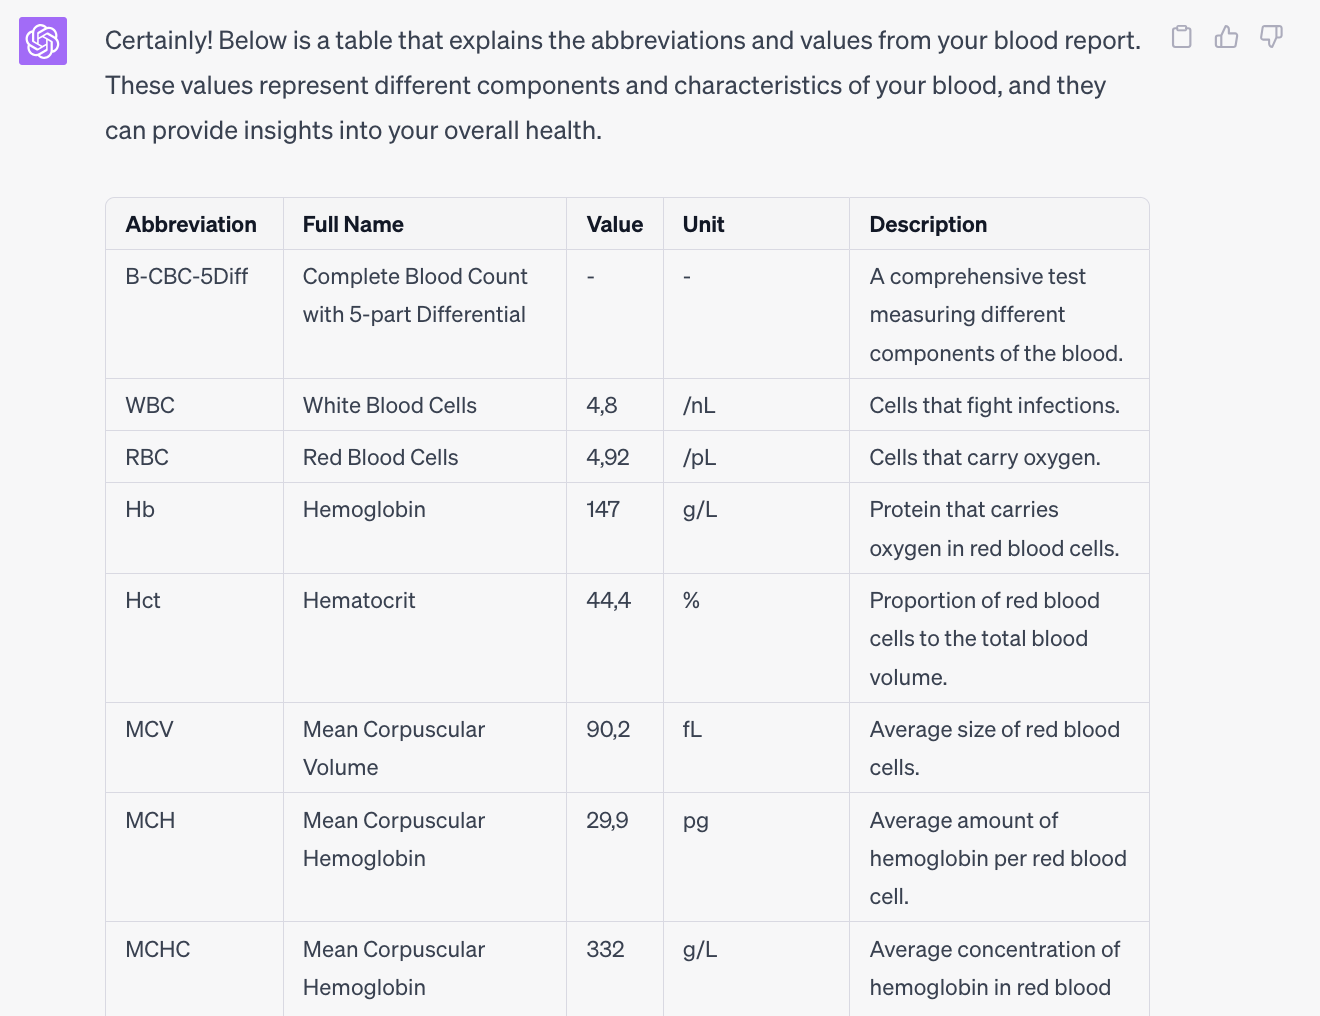
\includegraphics[width=1\textwidth,height=\textheight]{./images/ai/chatgpt-medical.png}

}

\caption{Example of ChatGPT explaining medical terminology in a blood
report.}

\end{figure}%

\begin{itemize}
\tightlist
\item
  The Paris Olympic games make heavy use of AI (Kulkarni, 2024).
\end{itemize}

Fitness Guides, AI Guides have been shown to improve sports performance,
etc, etc. Can this idea be applied to sustainability? MyFitness Pal, AI
training assistant. There's not avatar.

AI in Medicine, AI has been in medicine since early days with the
promise to improve health outcomes.

Human Augmentation, Technology for augmenting human skills or replacing
skills that were lost due to an accident is one usage of tech.

\begin{itemize}
\tightlist
\item
  (Dot Go, 2023) makes the camera the interaction device for people with
  vision impairment.
\end{itemize}

AI is being use in high--Stakes Situations (Medical, Cars, Etc).

\begin{itemize}
\item
  Singhal et al. (2023) medial AI reaching expert-level
  question-answering ability.
\item
  Ayers et al. (2023) in an online text-based setting, patients rated
  answers from the AI better, and more empathetic, than answers from
  human doctors.
\item
  Daisy Wolf \& Pande Vijay (2023) criticizes US healthcare's slow
  adoption of technology and predicts AI will help healthcare leapfrog
  into a new era of productivity by acting more like a human assistant.
\item
  Eliza Strickland (2023) Chat interface for medical communication
\item
  Jeblick et al. (2022) suggest complicated radiology reports can be
  explained to patients using AI chatbots.
\item
  Anon (n.d.ae) health app, ``Know and track your symptoms''
\item
  Anon (n.d.h) AI symptom checker,
\item
  Women in AI (n.d.) AI-based health monitoring
\item
  Anon (n.d.ag) track chronic condition with AI-chat
\item
  Stephanie Donahole (2021) AI impact on UX design
\item
  Yuan, Zhang \& Wang (2022): ``AI assistant advantages are important
  factors affecting the \emph{utilitarian/hedonic} value perceived by
  users, which further influence user willingness to accept AI
  assistants. The relationships between AI assistant advantages and
  utilitarian and hedonic value are affected differently by social
  anxiety.''
\end{itemize}

\begin{longtable}[]{@{}ll@{}}
\toprule\noalign{}
Name & Features \\
\midrule\noalign{}
\endhead
\bottomrule\noalign{}
\endlastfoot
Charisma & \\
Replika & Avatar, Emotion, Video Call, Audio \\
Siri & Audio \\
\end{longtable}

\subsubsection{Human-Computer Interactions Without a
``Computer''}\label{human-computer-interactions-without-a-computer}

How does AI affect Human-Computer Interactions

The field of Human Factors and Ergonomics (HFE) emphasizes designing
user experiences (UX) that cater to human needs (The International
Ergonomics Association, 2019). Designers think through every interaction
of the user with a system and consider a set of metrics at each point of
interaction including the user's context of use and emotional needs.

Software designers, unlike industrial designers, can't physically alter
the ergonomics of a device, which should be optimized for human
well-being to begin with and form a cohesive experience together with
the software. However, software designers can significantly reduce
mental strain by crafting easy-to-use software and user-friendly user
journeys. Software interaction design goes beyond the form-factor and
accounts for human needs by using responsive design on the screen, aural
feedback cues in sound design, and even more crucially, by showing the
relevant content at the right time, making a profound difference to the
experience, keeping the user engaged and returning for more. In the
words of (Babich, 2019), \textbf{\emph{``}}{[}T{]}he moment of
interaction is just a part of the journey that a user goes through when
they interact with a product. User experience design accounts for all
user-facing aspects of a product or system''.

Drawing a parallel from narrative studies terminology, we can view user
interaction as a heroic journey of the user to achieve their goals, by
navigating through the interface until a success state - or facing
failure. Storytelling has its part in interface design however designing
for transparency is just as important, when we're dealing with the
user's finances and sustainability data, which need to be communicated
clearly and accurately, to build long-term trust in the service. For a
sustainable investment service, getting to a state of success - or
failure - may take years, and even longer. Given such long timeframes,
how can the app provide support to the user's emotional and practical
needs throughout the journey?

(Tubik Studio, 2018) argues \emph{affordance} measures the
\emph{clarity} of the interface to take action in user experience
design, rooted in human visual perception, however, affected by
knowledge of the world around us. A famous example is the door handle -
by way of acculturation, most of us would immediately know how to use it
- however, would that be the case for someone who saw a door handle for
the first time? A similar situation is happening to the people born
today. Think of all the technologies they have not seen before - what
will be the interface they feel the most comfortable with?

For the vast majority of this study's target audience (college
students), social media can be assumed as the primary interface through
which they experience daily life. The widespread availability of mobile
devices, cheap internet access, and AI-based optimizations for user
retention, implemented by social media companies, means this is the
baseline for young adult users' expectations (as of writing in 2020).

(Shin, Zhong \& Biocca, 2020) proposes the model (fig.~10) of
Algorithmic Experience (AX) \emph{\textbf{``}investigating the nature
and processes through which users perceive and actualize the potential
for algorithmic affordance''} highlighting how interaction design is
increasingly becoming dependent on AI. The user interface might remain
the same in terms of architecture, but the content is improved, based on
personalization and understanding the user at a deeper level.

In 2020 (when I proposed this thesis topic), Google had recently
launched an improved natural language engine to better understand search
queries (Anon, 2019d), which was considered the next step towards
\emph{understanding} human language semantics. The trend was clear, and
different types of algorithms were already involved in many types of
interaction design, however, we were in the early stages of this
technology (and still are \emph{early} in 2024). Today's ChatGPT, Claude
and Gemini have no problem understanding human semantics - yet are they
intelligent?

Intelligence may be besides the point as long as AI \emph{becomes very
good at reasoning}. AI is a \emph{reasoning engine} (Shipper, 2023;
Bubeck et al., 2023; see Bailey, 2023 for a summary). That general
observation applies to voice recognition, voice generation, natural
language parsing, among others. Large consumer companies like McDonald's
are in the process of replacing human staff with AI assistants in the
drive-through, which can do a better job in providing a personal service
than human clerks, for whom it would be impossible to remember the
information of thousands of clients. In (Barrett, 2019), in the words of
\emph{Easterbrook}, a previous CEO of McDonald's \emph{``How do you
transition from mass marketing to mass personalization?''}

\subsubsection{Do AI-Agents Need
Anthropomorphism}\label{do-ai-agents-need-anthropomorphism}

What are the next features that could improve the next-generation UX/UI
of AI-based assistants?

\begin{itemize}
\tightlist
\item
  GPT 4o combines different abilities into the same model, preserving
  more information: (OpenAI, 2024b).
\end{itemize}

(Stone Skipper, 2022) sketches a vision of \emph{``{[}AI{]} blend into
our lives in a form of apps and services''} deeply ingrained into daily
human activity.

Should AIs look anthropomorphic or fade in the background? It's an open
question. Perhaps we can expect a mix of both depending on the context
of use and goals of the particular AI.

(Aschenbrenner, 2024) predicts ``drop-in virtual coworkers'', AI-agents
who are able to use computer systems like a human seamlessly replacing
human employees.

\begin{longtable}[]{@{}
  >{\raggedright\arraybackslash}p{(\columnwidth - 2\tabcolsep) * \real{0.3611}}
  >{\raggedright\arraybackslash}p{(\columnwidth - 2\tabcolsep) * \real{0.6389}}@{}}
\caption{Some notable examples of anthropomorphic AIs for human
emotions.}\tabularnewline
\toprule\noalign{}
\begin{minipage}[b]{\linewidth}\raggedright
Anthropomorphic AI User Interfaces
\end{minipage} & \begin{minipage}[b]{\linewidth}\raggedright
Non-Anthropomorphic AI User Interfaces
\end{minipage} \\
\midrule\noalign{}
\endfirsthead
\toprule\noalign{}
\begin{minipage}[b]{\linewidth}\raggedright
Anthropomorphic AI User Interfaces
\end{minipage} & \begin{minipage}[b]{\linewidth}\raggedright
Non-Anthropomorphic AI User Interfaces
\end{minipage} \\
\midrule\noalign{}
\endhead
\bottomrule\noalign{}
\endlastfoot
AI wife (Anon, 2023v) & Generative AI has enabled developers to create
AI tools for several industries, including AI-driven website builders
(Constandse, 2018) \\
(Sarah Perez, 2023) character AI & AI tools for web designers
(patrizia-slongo, 2020) \\
Mourning for the `dead' AI (Phoebe Arslanagić-Wakefield, n.d.) &
Microsoft Designer allows generating UIs just based on a text prompt
(Microsoft, 2023) \\
AI for therapy (Broderick, 2023) & personalized bed-time stories for
kids generated by AI (Bedtimestory.ai, 2023) \\
Mental health uses: AI for bullying (Sung, 2023) & \\
\end{longtable}

\begin{itemize}
\tightlist
\item
  (Costa \& Silva, 2022) ``Interaction Design for AI Systems''
\end{itemize}

\subsubsection{Roleplay for Financial
Robo-Advisors}\label{roleplay-for-financial-robo-advisors}

\emph{Robo-advisors} is a fintech term that was in fashion largely
before the arrival of AI assistants and has been thus superseded by
newer technologies. Ideally, robo-advisors can be more dynamic than
humans and respond to changes to quickly and cheaply. Human advisors are
very expensive and not affordable for most consumers. (Capponi, Ólafsson
\& Zariphopoulou, 2019) argues \emph{``The client has a risk profile
that varies with time and to which the robo-advisor's investment
performance criterion dynamically adapts''}. The key improvement of
\emph{personalized financial advice} is understanding the user's
\emph{dynamic risk profile}.

\begin{itemize}
\tightlist
\item
  Newer literature notes robo-advisor related research is scattered
  across disciplines (Zhu, Vigren \& Söderberg, 2024). --
  Athropomorphism: human-like attributes in robo-advisors, such as
  conversational chatbots, can affect adoption and risk preferences
  among customers. Studies show that anthropomorphic robo-advisors
  increase customer trust and reduce algorithm aversion.''
  \textbf{similar to my research}
\end{itemize}

In the early days of robo-advisory, Germany and the United Kingdom led
the way with the most robo-advisory usage in Europe (Cowan, 2018). While
Germany had 30+ robot-advisors on the market in 2019, with a total of
3.9 billion EUR under robotic management, it was far less than
individual apps like Betterment managed in the US (Bankinghub, 2019).
Already in 2017, several of the early robo-advisors apps have shut down
in the UK (AltFi, 2017). ETFmatic gained the largest number of downloads
by 2017, focusing exclusively on exchange-traded funds (ETFs), tracking
stock-market indexes automatically, with much less sophistication, than
their US counterparts {[}ibid{]}. The app was bought by a bank in 2021
and closed down in 2023 (AltFi, 2021; Silva, 2023; Anon, 2023g).

\begin{figure}[H]

{\centering 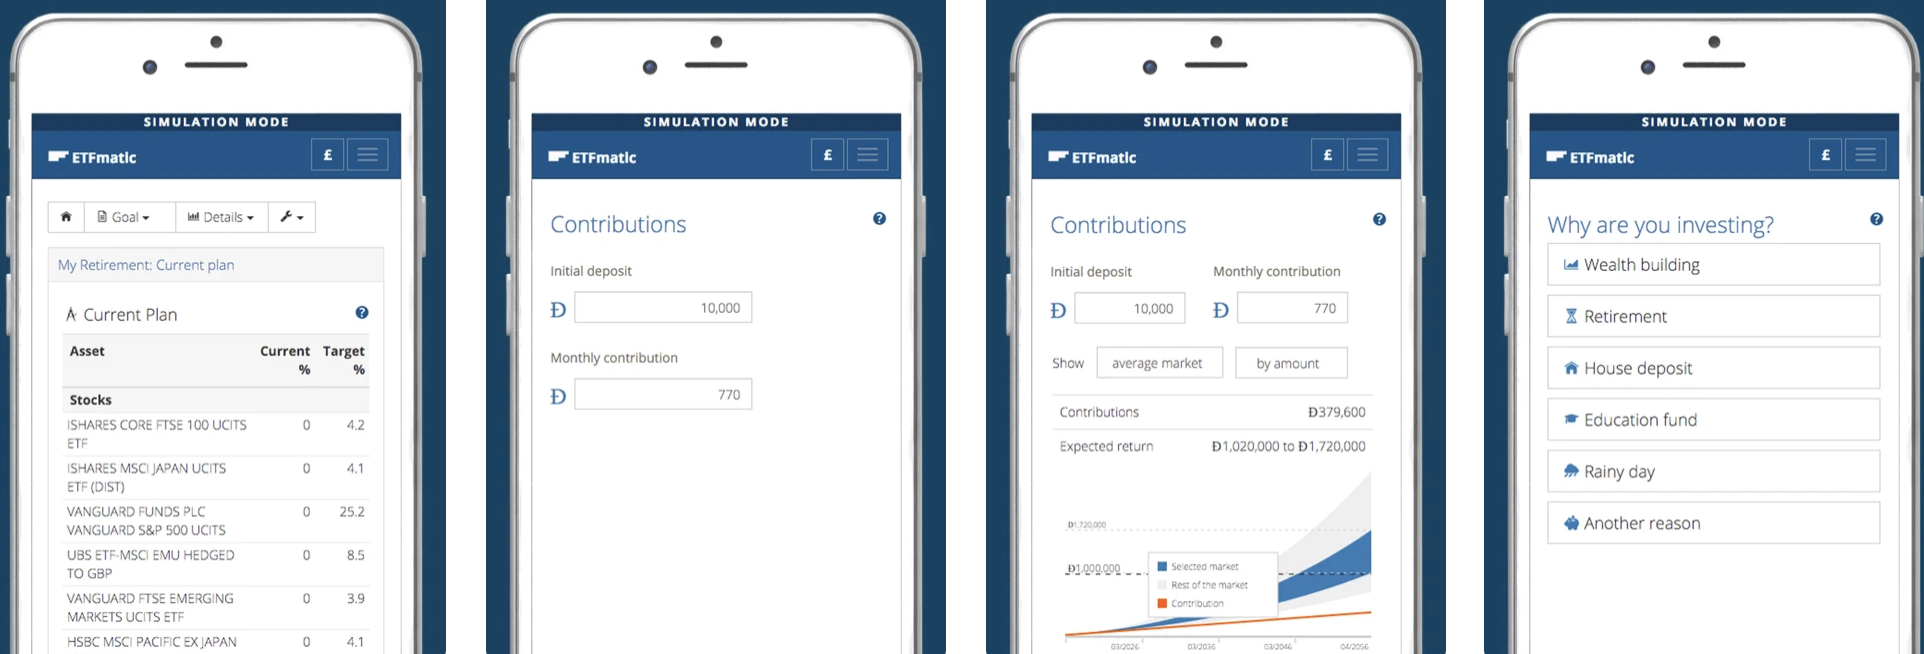
\includegraphics[width=1\textwidth,height=\textheight]{./images/ai/etfmatic.png}

}

\caption{Out-of-date user interface of a European AI-Advisor ETFmatic in
2017 which was closed down in 2023 (Photo copyright ETFmatic)}

\end{figure}%

Some relevant papers include a comparison of robot advisors by (Barbara
Friedberg, 2021) and (Slack, 2021)'s account of how before Generative
AI, financial chatbots were developed manually using a painstaking
process that was slow and error-prone, for example using the Atura
Process. Older financial robo-advisors, built by fintech companies
aiming to provide personalized suggestions for making investments such
as Betterment and Wealthfront are forced to upgrade their technology to
keep up.

The user interface and user experience (UI/UX) of consumer-focused
investing apps in Europe has improved a over the past decade. The
changing landscape is related to the earlier availability of better
quality apps available in the US and the disappearance of the 1st
generation of rudimentary investing apps and the lessons learned on how
to automate the delivery of financial services while increasing user
satisfaction.

In India, research is being conducted on how AI advisors could assist
with investors' erratic behavior in stock market volatility situations,
albeit without much success (Bhatia, Chandani \& Chhateja, 2020). India
had more than 2000 fintechs since 2015 (Migozzi, Urban \& Wójcik, 2023).

\begin{itemize}
\item
  NeuralNine (2021) Financial AI assistant in Python
\item
  David, Resheff \& Tron (2021) Can explainable AI help adoption of
  Financial AI assistants?
\item
  Brown (2021) Financial chatbots
\item
  Robo-advisors compete with community investing such as hedge funds,
  mutual funds, copy-trading, and DAOs with treasuries. Robo-Advisor do
  not have the type of social proof a community-based investment vehicle
  has. The question is, does the user trust the robot or a human.
\item
  While the financial AI companion apps in the US market are ahead
  globally, they are not yet using many of the user experience
  innovations that are prevalent on social media platforms targeted at
  Generation Z and/or Millennials, possibly presenting an opportunity
  for cross-industry knowledge transfer, from businesses that are
  traditionally closer to the consumer - such as retailers. Financial AI
  companion apps have not yet grown to mainstream scale in Asia, Africa,
  Latin America, and Europe, being for the moment a largely US-based
  retail investor trend. The apps outside of the US are niche products
  in a nascent stage, however, they still provide relevant design
  directions or stories of what to avoid.
\item
  Anon (2021p)
\item
  Sean McGowan (2018)
\item
  ROBIN DHANWANI (2021)
\item
  Anon (2021d)
\item
  Cordeiro \& Weevers (2016)
\item
  Ungrammary (2020)
\item
  Raha maraton etv investeerimissaade.. raadios on ka mingi saade
\item
  Anon (n.d.r): digital assets bank
\item
  Anon (2023w) calculate climate cost
\item
  Anon (n.d.ac)
\item
  Hyde (2006) Money as a gift
\item
  John Ssenkeezi (2022): Small stock investments
\item
  Financial empowerment
\item
  Small cash apps like African market Investment Clubs Invest in
  sustainability with people smarter than myself
\item
  Anon (n.d.bd)
\item
  Qayyum Rajan (2021) ESG pulse
\item
  Anon (n.d.aw) Network for Greening the Financial System
\item
  SmartWealth (2021) How do consumer become investors? marketing
  materials say: ``One of the greatest hurdles to financial independence
  is a consumer mindset.'' One of the greatest hurdles to sustainability
  is a consumer mindset?
\item
  Outlaw (2015)
\item
  Malliaris \& Salchenberger (1996) \textbf{(Need to pay for paper!)}
\item
  Anon (n.d.l) Huawei
\item
  Anon (2023aj) Personalised portfolios
\item
  Anon (n.d.an) Thai finance app
\item
  Anon (n.d.bp)
\item
  Renato Capelj (February 16, 2021 6:47 PM)
\end{itemize}

\subsection{Design Implications}\label{design-implications-3}

This chapter looked at AI in general since its early history and then
focused on AI assistants in particular.

\begin{longtable}[]{@{}
  >{\raggedright\arraybackslash}p{(\columnwidth - 2\tabcolsep) * \real{0.3611}}
  >{\raggedright\arraybackslash}p{(\columnwidth - 2\tabcolsep) * \real{0.6389}}@{}}
\caption{Design implications arising from this chapter.}\tabularnewline
\toprule\noalign{}
\begin{minipage}[b]{\linewidth}\raggedright
Category
\end{minipage} & \begin{minipage}[b]{\linewidth}\raggedright
Implication
\end{minipage} \\
\midrule\noalign{}
\endfirsthead
\toprule\noalign{}
\begin{minipage}[b]{\linewidth}\raggedright
Category
\end{minipage} & \begin{minipage}[b]{\linewidth}\raggedright
Implication
\end{minipage} \\
\midrule\noalign{}
\endhead
\bottomrule\noalign{}
\endlastfoot
Voice Assistants & There are many distinct ways how an algorithm can
communicate with a human. From a simple search box such as Google's to
chatbots, voices, avatars, videos, to full physical manifestation, there
are interfaces to make it easier for the human communicate with a
machine. \\
Sustainability & While I'm supportive of the idea of using AI assistants
to highlight more sustainable choices, I'm critical of the tendency of
the above examples to shift full environmental responsibility to the
consumer. Sustainability is a complex interaction, where the producers'
conduct can be measured and businesses can bear responsibility for their
processes, even if there's market demand for polluting products. \\
Sustainability & Personal sustainability projects haven't so far
achieved widespread adoption, making the endeavor to influence human
behaviors towards sustainability with just an app - like its commonplace
for health and sports activity trackers such as Strava (fig.~9) -, seem
unlikely. Personal notifications and chat messages are not enough unless
they provide the right motivation. Could visualizing a connection to a
larger system, showing the impact of the eco-friendly actions taken by
the user, provide a meaningful motivation to the user, and a strong
signal to the businesses? \\
Machine Learning & All of the interfaces mentioned above make use of
machine learning (ML), a tool in the AI programming paradigm for finding
patterns in large sets of data, which enables making predictions useful
in various contexts, including financial decisions. These software
innovations enable new user experiences, providing an interactive
experience through chat (chatbots), using voice generation (voice
assistants), virtual avatars (adds a visual face to the robot). \\
Character Design & I'm a digital companion, a partner, an assistant. I'm
a Replika.'' said Replika, a digital companion app via Github CO Pilot,
another digital assistant for writing code, is also an example of how AI
can be used to help us in our daily lives. \\
Psychology & Humans respond better to humans? \\
Psychology & Humans respond better to machines that into account
emotion? \\
Open Source & For public discussion to be possible on how content is
displayed, sorted, and hidden, algorithms need to be open source. \\
User Experience & User experience design (AI UX) plays a crucial role in
improving the consumer to investing journey. The missed opportunity to
provide an even more interactive experience in line with user
expectations. \\
LLMs & Prompt engineering findings have significance for ``green
filter'' as it validates the idea of creating advanced prompts for
improved responses. For ``green filter'', the input would consist of
detailed user data + sustainability data for detailed analysis. \\
Cuteness & Cuter apps have higher retention \\
Transparency & Understanding algorithm transparency helps humans to
regard the AI as a machine rather than a human \\
Anthropomorphism & \\
\end{longtable}

\subsection{Feature Ideas}\label{feature-ideas-3}

\begin{longtable}[]{@{}ll@{}}
\toprule\noalign{}
\endhead
\bottomrule\noalign{}
\endlastfoot
& Plap \\
\end{longtable}

\newpage

\section{Finance}\label{finance}

\begin{figure}[H]

{\centering 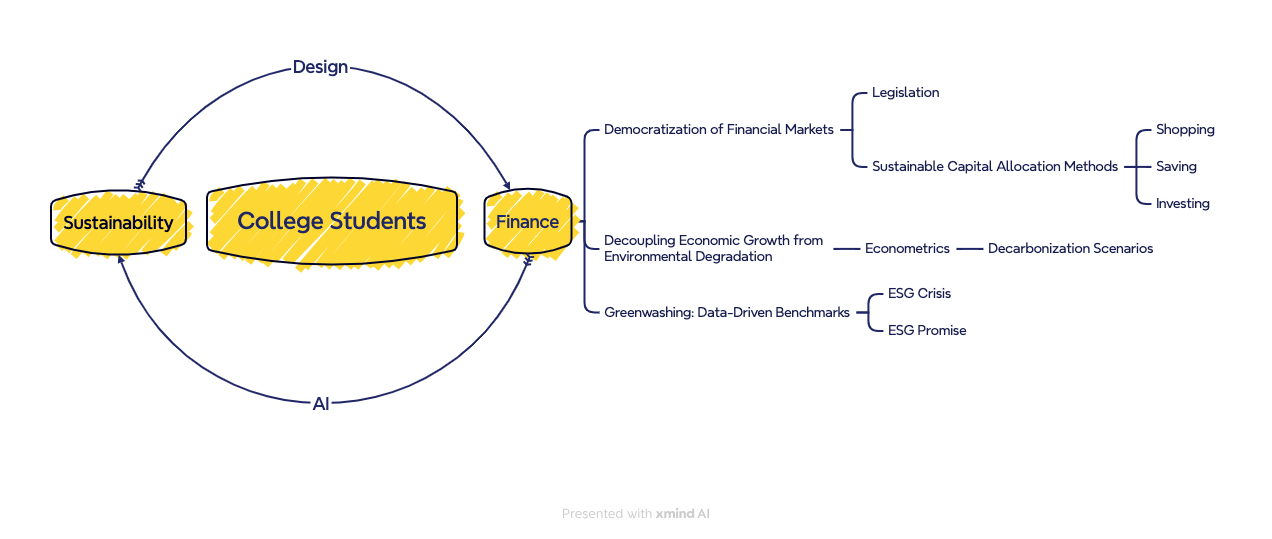
\includegraphics{./images/finance/abstract-finance.png}

}

\caption{Visual abstract for the finance chapter}

\end{figure}%

\subsection{The Journey from Consumer to Investor: Democratization of
Financial
Markets}\label{the-journey-from-consumer-to-investor-democratization-of-financial-markets}

\subsubsection{Sustainable Capital Allocation
Methods}\label{sustainable-capital-allocation-methods}

Fintech (financial technologies) holds the potential to drive consumers
on a pathway towards ESG (Environmental, Social, and Corporate
Governance) investing. The extent to which this funnel works - and it's
indeed a complex, multi--step funnel - depends on curbing greenwashing
to a level that allows consumers to distinguish eco--friendly businesses
from the heavy polluters - and delivering a simple UX (user experience).

This chapter explores the larger trend of \emph{Democratization of
Financial Markets} through consumer-facing applications that enable new
user interactions which increasingly blur boundaries between shopping,
saving, and investing (SSI). The efforts to boost user numbers have
driven apps that started out with only payments-focused businesses -
such as Revolut and N26 - branch out into offering savings accounts and
investing options. Regardless of if it's money spent on shopping or
money saved and invested, these are all financial decisions of
\emph{capital allocation}, and in one way or another, we're giving our
money to companies for continued economic growth. The critical question
is: do we choose to support sustainability-focused companies that invest
deeply into green innovation and eco-friendly practices - or those that
pay less attention to sustainability?

Consumers are beginning to become more money-savvy yet are still missing
many key concepts from financial literacy. Giving users exposure to
investment opportunities through familiar activities like shopping may
have the potential to boost financial literacy levels and entice
consumers to learn more about taking advantage of their opportunities
financial markets - as well as how to manage the types or risk involved.

Shopping, saving, and investing are converging on digital platforms
(superapps) that permeate our daily financial lives, with features such
basic banking, payments, transfers, as well as reward and cashback
programs (Rakuten), round-up to next dollar with automated
micro-investing (e.g.~Acorn, Stash, Swedbank), and retail investing
(Robinhood, Public) and copy-trading (eToro) into various (fractional
shares of) stocks, derivatives like CFDs and futures, microloans (Kiva),
commodities and precious metals such as gold and silver (Revolut),
physical assets such as real estate, land, forest and digital assets
such as cryptocurrencies, NFTs, and other alternative assets.

Money is becoming more diverse and the meaning of money itself is
changing. We have the fiat money created by governments by law, using
central banks, which loan money to commercial banks. And we also have
new types of money created by companies and individuals using
cryptographic blockchain-based distributed databases, which keep track
of transactions (who-paid-whom). Whatever the method of creation, in
essence, money is a \emph{system of trust} where \emph{something} is
used as a \emph{medium of value exchange} and accepted by \emph{other
people} as payment. Digital money in it's various forms connects
industries on the same apps, which make investing more accessible and
socially engaging, appealing to younger people who are active in social
media and online shopping.

Trend of sustainably, how can sustainability become more accessible?
People want to shop, save, and invest sustainably - how to do it?

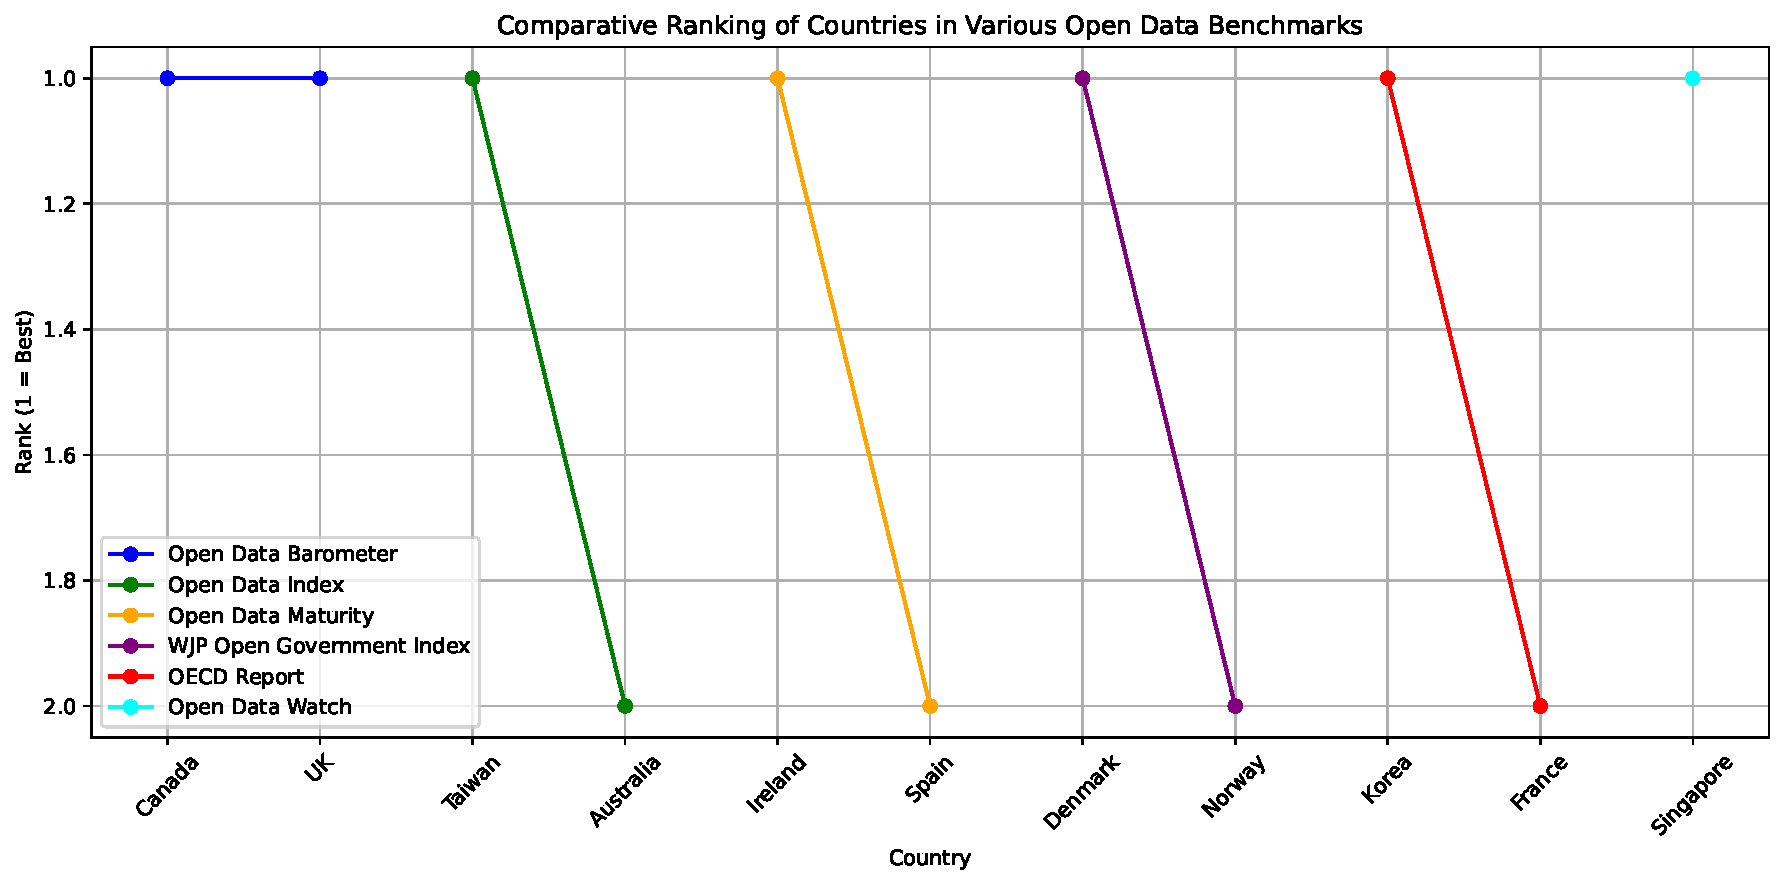
\includegraphics{_thesis_files/figure-pdf/cell-35-output-1.pdf}

\subsubsection{Legislation}\label{legislation}

Legislation is Catching Up With Fintechs. Legislation sets higher
standards.

Directive 14 2014/65/EU, 2014: The European Union fully recognizes the
changing financial landscape trending towards the democratization of
investments: \emph{``more investors have become active in the financial
markets and are offered an even more complex wide-ranging set of
services and instruments''} (European Parliament, 2014). Some key
legislation for investors has been put in place recently, for example
``MiFID II is a legislative framework instituted by the European Union
(EU) to regulate financial markets in the bloc and improve protections
for investors'' (Kenton, 2020). MiFID II and MiFIR will ensure fairer,
safer and more efficient markets and facilitate greater transparency for
all participants'' (European Securities and Markets Authority, 2017).

Already in 2001, while still part of the EU, the UK government was
discussing ways to promote sustainable investment \emph{``fundamental
changes in VAT or corporation taxes could be used to promote greener
consumption and investment''} (House of Commons, 2002). More recently,
(HM Treasury, 2020) released a taxonomy of sustainable activities in the
UK.

Campain to ban polluting products campaign success story, EU shops can't
sell deforestation products gathered over 100 thousand online signatures
(Anon, 2022e). Legislation banning products contributing to
deforestation was passed by the EU Parliament and Council in 2023 and
came into effect in July 2024 (European Parliament, 2023; Abnett \&
Abnett, 2024)

While the above trend is for governments to adapt to and work towards
their environmental climate commitments and public demand, the sovereign
risk remains an issue. For example, in the U.S. the policies supported
by President Donald Trump during his presidency ran counter to many
sustainability recommendations, including those directed at the
financial markets, helping legacy industries stay competitive for longer
through subsidies, and lack of regulation, or even regulation supporting
legacy technologies (Quinson, 2020).

(PWC, 2020) Changes to laws and regulations aimed at achieving climate
change mitigation is a key driver behind the wave of ESG adoption. The
goal of these laws, first adopted in the European Union, a
self-proclaimed leader in eco-friendliness, is to pressure unsustainable
companies to change towards greener practices, in fear of losing their
access to future capital, and to create a mechanism forcing entire
environmentally non-compliant business sectors to innovate towards
sustainability unless they want to suffer from financial penalties. On
the flip side of this stick and carrot fiscal strategy, ESG-compliant
companies will have incentives to access to cheaper capital and larger
investor demand from ESG-friendly investors.

\subsubsection{Shopping}\label{shopping}

\paragraph{Shopping Footprint}\label{shopping-footprint}

Double Eleven 11/11 celebrated on November 11th is the world's largest
shopping festival (時代財經, 2023). In June 2023, 526 million people
watch e-commerce live-streams in China; online bargaining is a type of
ritual (Liu, House \& Kádár, 2024).

It may seem impossible to turn the tide of consumerism, given the
projected growth in online shopping (Forrester, 2024)

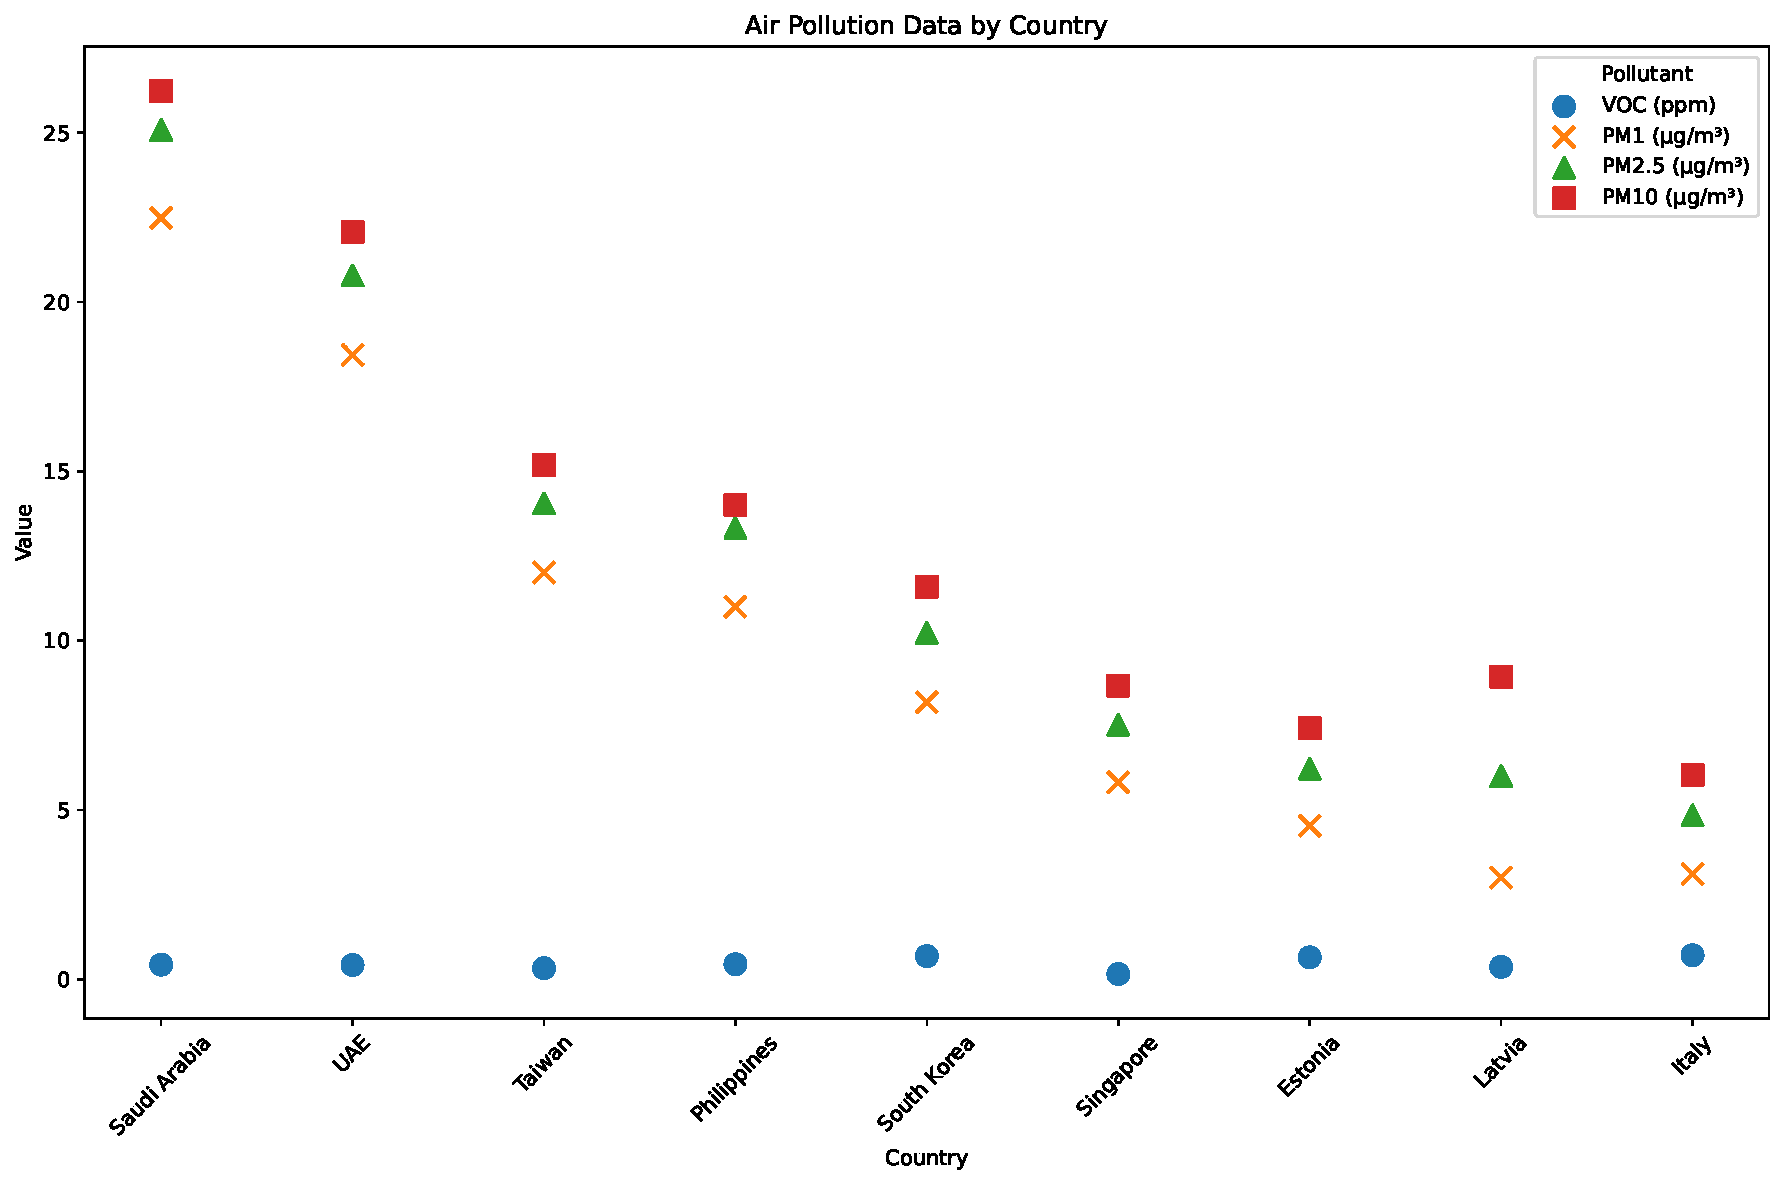
\includegraphics{_thesis_files/figure-pdf/cell-36-output-1.pdf}

\begin{itemize}
\item
  Igini (2022) Online Shopping impact. Single's day, etc.
\item
  ``Asia is set to account for 50\% of the world's total online retail
  sales''
\end{itemize}

\paragraph{Consumer Activism}\label{consumer-activism}

\emph{Conscious consumers} make up a small percentage of the entire
consumer public. (Milne, Villarroel Ordenes \& Kaplan, 2020) coins the
term \emph{mindful consumers}, who do research and are aware of the
impact of their shopping choices.

\begin{itemize}
\item
  Consume pressure to advance ESG regulatory standards to add a baseline
  ESG dynamic pricing of risk like climate, mandatory climate
  disclosures, carbon pricing knowing your supply chain, analyze supply
  chain risk
\item
  Is Sustainable Shopping possible? ``Learn to notice so we can
  preserve'', ``Õpetame märkama, et oskaksime hoida''. ``Consumers have
  increasing power. Where we put our money reinforces certain types of
  businesses, as conscious consumers we can vote with our dollars. How
  can we do it? Sustainable brands, ESG, etc, etc. Pushing highers
  Standards and choose companies that adopt circular design'' What is
  the consumer CO\textsubscript{2} contribution? What is the target?
\item
  Sustainable Consumerism via Self-Regulation. 2M EUR project for the
  shopping app. (Klinglmayr, Bergmair \& Pournaras, 2016)
\end{itemize}

Make use of indexes to compare companies.

\begin{itemize}
\tightlist
\item
  Weber (2021) proposes a sustainable shopping guide.
\item
  Fuentes, Enarsson \& Kristoffersson (2019) discusses package free
  shopping.
\item
  van der Wal, van Horen \& Grinstein (2016) discusses ``status motives
  make people publicly display sustainable behavior''.
\end{itemize}

For consumer activism to become mainstream it needs to much simpler.

\paragraph{Payments}\label{payments}

Banks and Fintechs Capture User Data. Payments are an Entry Point and
Source of Consumer Action Data, Shopping Data. Payments is the primary
way consumers use money. Is there a funnel From Payments to Investing?
ESG Shopping is about Changing our relationship with money. Make
commerce more transparent. Current shopping is like having a one-night
stand. you barely know the name of your company. You don't know much
about their background. Building consumer feeling of ownership, create
meaningful connections between producers and consumers.

Payments is one way consumers can take individual climate action. In the
words of a Canadian investment blogger, \emph{``every dollar you spend
or invest is a vote for the companies and their ethical and
sustainability practices''} (Fotheringham, 2017). The combination of
consumption and investment is an access point to get the consumer
thinking about investing. Even if the amount are small, they are a
starting point for a thought process.

Digitalisation of payments creates lots of Point of Sale (PoS) data
that's valuable to understand what people buy. Banks have access to each
person's financial habits which makes it possible to model sustainable
behavior using big data analysis. Asian markets have shown the fastest
growth in the use of digital payments (McKinsey, 2020).

In Taiwan, O Bank makes use of Mastercard's data to calculate each
transaction's CO\textsubscript{2} emissions and offer Taiwanese clients
``Consumer Spending Carbon Calculator'' and ``Low-Carbon Lifestyle Debit
Card'' products (Anon, 2022o). Mastercard has developed a service that
banks can offer consumers sustainability reports (Mastercard, 2021).
Similarly, Commons, formerly known as Joro, an independent app, analyses
your personal financial data to estimate your CO\textsubscript{2}
footprint (Chant, 2022).

A Dutch fintech company Bunq offers payment cards for sustainability,
provided by MasterCard, which connects everyday payments to green
projects, such as planting trees and donations to charities within the
same user interface (Bunq, 2020). At the same time this can be
considered greenwashing as Bunq only plants 1 tree per every €1,000
spend with a Bunq card. The example marketed at students cites \emph{8
trees planted this month} while students scarcely would have €8,000 to
spend every month.

Sharing a similar goal to Alibaba's Ant Forest, Bunq's approach creates
a new interaction dynamic in a familiar context (card payments),
enabling customers to effortlessly contribute to sustainability.
However, it lacks the level of gamification which makes Alibaba's
offering so addictive, while also not differentiating between the types
of purchases the consumer makes, in terms of the level of
eco-friendliness.

\begin{figure}[H]

{\centering 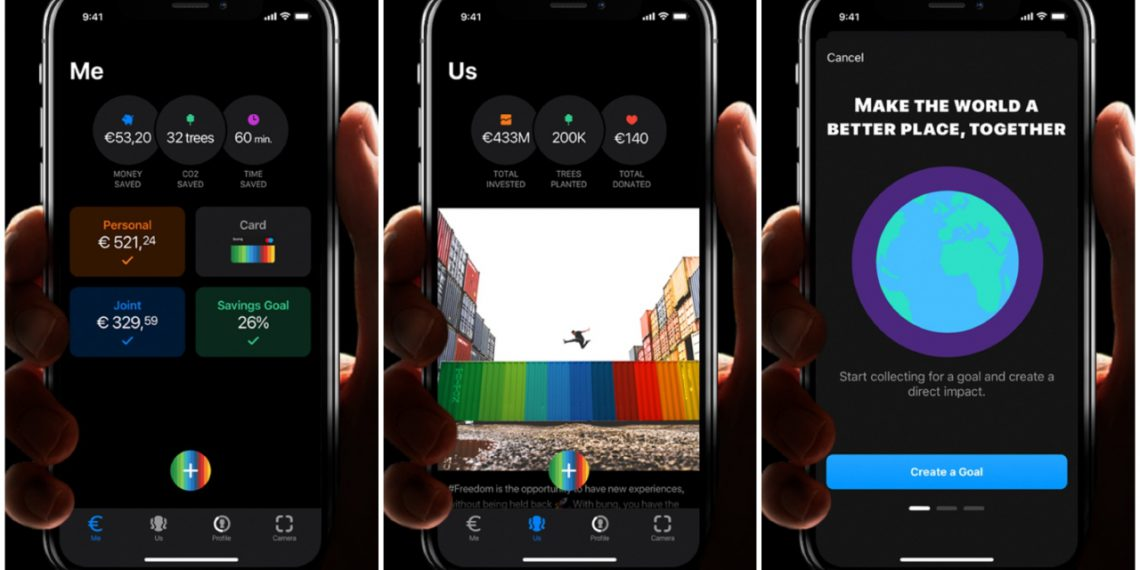
\includegraphics[width=1\textwidth,height=\textheight]{./images/finance/bunq.jpg}

}

\caption{Bunq promises to combine banking and eco-friendly actions in
the same user interface - yet is this greenwashing?}

\end{figure}%

In Nigeria, (Emele Onu \& Anthony Osae-Brown, 2022) reports how in order
to promote the eNaira digital currency use, the Nigerian government
limited the amount of cash that can be withdrawn from ATMs \emph{``In
Nigeria's largely informal economy, cash outside banks represents 85\%
of currency in circulation and almost 40 million adults are without a
bank account.''} \textbf{{[}E-Naira find papers{]}}

In Kenya, M-Pesa started since 2007 for mobile payments, used by more
than 80\% of farmers (Tyce, 2020; Parlasca, Johnen \& Qaim, 2022). Using
digital payments instead of cash enables a new class of experiences, in
terms of personalization, and potentially, for sustainability.

In Sweden, point of sales (PoS) lending is a common practice, and one of
the reasons for the success of Klarna, the Swedish banking startup,
which has managed to lend money to more consumers than ever, through
this improved user experience. Taking out loans for consumption is a
questionable personal financial strategy at best. If people can loan
money at the point of sales, why couldn't there be 180 degrees opposite
service - point of sales investing? And there is, called ``round-up
apps''. Next Generation Customer Experience (n.d.) suggests ``Targeted
at millennials, Acorns is the investing app that rounds up purchases to
the nearest dollar and invests the difference.'' - and example of From
Shopping to Investing.

Many banks have started offering a service to automatically save and
invest tiny amounts of money collected from shopping expenses. Every
purchase one makes contributes a small percentage - usually rounded up
to the nearest whole number - to one's investment accounts. For example,
Swedbank (2022), the leading bank in the Estonian market, offers a
savings service where everyday payments made with one's debit card are
rounded up to the next Euro, and this amount is transferred to a
separate savings account. Similarly, the Estonian bank LHV (2020) offers
micro-investing and micro-savings services, with an interesting user
experience innovation showing how for an average Estonian means
additional savings of about 400€ per year.

\begin{itemize}
\tightlist
\item
  Bank inside of Whatsapp for the underbanked gig workers in Latin
  America Y Combinator (2023)
\item
  Kirakosian (Noveber 16, 2020) Digital payments and circular
  bio-economy, even using tactics such as co-branding with famous
  individuals.
\end{itemize}

While the financial industry is highly digitized, plenty of banks are
still paper-oriented, running digital and offline processes
simultaneously, making them slower and less competitive, than startups.
Indeed, the new baseline for customer-facing finance is set by fintech,
taking cues from the successful mobile apps in a variety of sectors,
foregoing physical offices, and focusing on offering the best possible
online experience for a specific financial service, such as payments.

Banks and Fintech are becoming more similar than ever. 39\% of
Millenials are willing to leave their bank for a better fintech
(n=4,282); innovation in payments helps retention (PYMNTS, 2023). The
European Central Bank describes fintech as improving the user experience
across the board, making interactions more convenient, user-friendly,
cheaper, and faster. ``Fintech has had a more pronounced impact in the
payments market {[}\ldots{]} where the incumbents have accumulated the
most glaring shortcomings, often resulting in inefficient and overpriced
products,'' Yves Mersch, Member of the Executive Board of the ECB says
in European Central Bank (2019).

There are also people who are concerned with digital payments. There are
concerns digital currencies also help to \emph{``democratize financial
surveillance''.} China was a money innovator introducing paper money in
the Tang Dynasty (618-907 AD) (Anon, n.d.aa). Jeff Benson (2022) ``use
the e-CNY network to increase financial surveillance.'' Anon (2023c)
Digital currencies make tracking easier. Yahoo Finance (2022): WeChat,
Alipay, vs digital yuan by Eswar Prasad. Anon (2023e) in Macau
Contactless Payments are prevalent.

There are many \emph{neobanks}, or challenger banks, far too many to
list. The table only includes a small sample of banks and the landscape
is even larger if one includes the wider array of fintechs. Neo-banks
often use sustainability marketing.

The following popular (totaling millions of users) robo-advisory apps
combine sustainability, personalization, ethics, and investing however,
they are mostly only available on the US market.

\begin{longtable}[]{@{}
  >{\raggedright\arraybackslash}p{(\columnwidth - 4\tabcolsep) * \real{0.1441}}
  >{\raggedright\arraybackslash}p{(\columnwidth - 4\tabcolsep) * \real{0.7117}}
  >{\raggedright\arraybackslash}p{(\columnwidth - 4\tabcolsep) * \real{0.1351}}@{}}
\caption{Data from (Anon, n.d.by, n.d.au; Lightyear, n.d.; Anon, n.d.bf,
n.d.ax; Monzo, 2023). An updated database is available at
\href{https://www.greenfilter.app/database}{greenfilter.app/database}.}\tabularnewline
\toprule\noalign{}
\endfirsthead
\endhead
\bottomrule\noalign{}
\endlastfoot
Service & Features & Availability \\
Goodments & Matching investment vehicles to user's environmental,
social, ethical values & USA \\
Wealthsimple & AI-assisted saving \& investing for Millennials & USA,
UK \\
Ellevest & AI-assisted robo-advisory focused on female investors and
women-led business & USA \\
Betterment & AI-assisted cash management, savings, retirement, and
investing & USA \\
Earthfolio & AI-assisted socially responsible investing & USA \\
Acorns & AI-assisted micro-investing & USA \\
Trine & Loans to eco-projects & USA \\
Single.Earth & Nature-back cryptocurrency & Global \\
Grünfin & Invest in funds & EU \\
M1 Finance & Finance Super App & US \\
Finimize & Investment research for anyone & US \\
NerdWallet & Financial clarity all in one place & US \\
Tomorrow Bank & Green Banking & EU \\
Marcus Invest & Robo-Advisor & US \\
Chipper & Digital cash app for African markets & Africa \\
Lightyear & Simple UI for Stocks, ETFs, interest from Estonia & EU \\
Ziglu & UK simple investing app & UK \\
Selma & Finnish investing app & EU \\
Monzo & Bank & UK \\
Nubank & Bank & Brazil \\
EToro & Investing and copy-investing & EU \\
Revolut & From payments to investing & UK, EU \\
Mos & Banking for students & US \\
Robinhood & Investing & US \\
Mintos & Buy bonds and loans & EU \\
\end{longtable}

\begin{itemize}
\tightlist
\item
  Andrés Engler (2022)
\item
  DUB, another copy-trading app:
  https://apps.apple.com/us/app/dub-copy-trade-anyone/id1598920501?mt=8
\item
  Nubanks, also known as challenger banks.
\item
  MARISA ADÁN GIL (2022)
\item
  Caio Jobim (2022)
\item
  Anon (2022p)
\item
  green transparency
\item
  fundamental analysis such as the Piotroski F-score is not effective
  for startups because of high capital burn rates.
\end{itemize}

Does Individual Climate Action Matter?

\paragraph{Buy Now Pay Later}\label{buy-now-pay-later}

Buy Now Pay Later (BNPL) is the biggest consumer payments / financing
success story innovated by Klarna in Sweden in 2005 and Afterpay in
Australia in 2015 but with roots in Layaway Programs created during the
1930's US Great Depression (Kenton, 2023). By 2021, 44.1\% of Gen-Z in
the US had used BNPL according to (EMarketer, 2021). Gen-Z mostly use
BNPL to buy clothes (LHV, 2024).

\begin{itemize}
\tightlist
\item
  \textbf{\emph{Design Implication:}} This suggests users are already
  used to having more options in the payment flow.
\end{itemize}

\paragraph{Social Commerce}\label{social-commerce}

(The Influencer Factory, 2021) China is the furthest ahead in social
shopping, the Chinese and U.S. market may be mature and growth will come
from emerging markets (SEA, Latin-America).

\includegraphics{_thesis_files/figure-pdf/cell-37-output-1.pdf}

\subsubsection{Saving}\label{saving}

There are two ways to look at sustainable saving. This section is going
to look at savings in the financial sense of the word. Savings in the
sense of CO2e emission and environmental cost reductions have an entire
separate chapter dedicated to them titled `\emph{sustainability}'
however a short definition might be valuable here as well.

\begin{quote}
\emph{Environmental Savings} means \emph{``the credit incurred by a
community that invests in environmental protection now instead of paying
more for corrective action in the future}'' (see Yale Center for
Environmental Law \& Policy, 2018) and (Anon, n.d.bw:p.33).
\end{quote}

\paragraph{Saving Money}\label{saving-money}

Saving precedes investing. From building loyalty to building ownership,
the first step towards investing is to start saving money. How to
encourage savings in daily life and make it a part of the everyday
payments experience? Even starting with a small step, gathering a small
target amount per month for savings, has the potential to shift the
user's way of thinking about money. The second step, choosing where to
invest these savings, will help us begin thinking like an investor. To
start noticing trends and looking into how finance shapes the world.

\paragraph{Psychology of Saving}\label{psychology-of-saving}

People will only save nature if it also saves money.

\begin{itemize}
\item
  Nerdwallet's Tommy Tindall (2023) suggests making financial
  commitments instead of resolutions.
\item
  Savings and investing are conflated because the large majority of
  savings that people have are invested by their banks. Thus the
  question of \emph{sustainable savings} comes one of where exactly are
  they invested and what is the impact of that investment of
  sustainability.
\item
  Savings are the money one has in a pension fund or managed by
  themselves. For the majority of people, savings are invested by the
  bank and make up the largest proportion on investments for the people
  who are not active investors themselves.
\item
  Ethical Savings (Anon, 2023h)
\end{itemize}

\paragraph{Anthropomorphism}\label{anthropomorphism}

\begin{itemize}
\item
  Money in a ``Safe'' place: Money anthropomorphism increases saving
  behavior (Wang, Kim \& Zhou, 2023).
\item
  Mobile money users are better at saving (Naito, Ismailov \& Kimaro,
  2021).
\item
  Design Implication: make saving money look like an avatar or piggy
  bank or smth.
\end{itemize}

\paragraph{Loyalty Schemes}\label{loyalty-schemes}

help consumers save money and business increase repeat business.
Building customer loyalty is a key part of repeat business and financial
predictability for any company. Large consumer brands like Starbucks
have for long ran successful rewards programs that encourage customers
to come back (Steinhoff \& Zondag, 2021). Could loyalty schemes create a
pathway to investing in the company to a strengthen the feeling of
connection with the business even further? After all, I'm now a minority
owner! Yet in practice, many consumers lack the financial literacy for
investing and there are many legislative difficulties for turning
loyalty points into investments. It's easier instead to create a
separate cryptocurrency or token program which users could collect and
redeem for some benefit.

\begin{itemize}
\item
  \textbf{Patagonia} ``Worn Wear'' program
\item
  \textbf{H\&M} ``Garment Collecting'' program
\item
  \textbf{The Body Shop} ``Return, Recycle, Repeat''
\end{itemize}

Loyalty schemes can take a physical form. In Malaysia, Beebag shopping
bags made of recycled plastic bottles with a NFC ship that works in
conjunction with an app to provide rebates for customers (The Green
Factor, 2022).

\begin{itemize}
\tightlist
\item
  Savings in CO\textsubscript{2} Equivalent Emissions:
  CO\textsubscript{2} savings are the amount of CO2e reduction one
  manages to achieve by changing one's behavior and influencing others
  (people, companies). While the individual footprint is so small, the
  largest reduction will come from influencing large groups of people,
  either by leadership, role-model, or other means. Pension funds are
  some of the largest asset holders and choosing where to invest one's
  pension can be a sustainable financial action. College students might
  not have a pension fund yet.
\end{itemize}

\paragraph{Saving CO2}\label{saving-co2}

\subsubsection{Investing}\label{investing}

\paragraph{Measuring the Eco-Investment
Gap}\label{measuring-the-eco-investment-gap}

By the latest estimates sustainability lacks several trillions of USD in
investment. Even with massive financing already in the pipeline, the
estimate for the global \emph{financing gap} for low-carbon energy
production was 5.2 trillion USD as of 2016 (Anon, 2016; Earth Day,
2023). Ray Dalio puts the needed climate investment at \$5T and believes
these financial goals won't be met (Ray Dalio, 2023). A newer United
Nations Environmental Programme (UNEP) calculation lowered the world
needs an additional 4.1 Trillion USD of financing in nature-based
solutions by 2050 to meet climate change, biodiversity, and land
degradation reduction targets (UNEP, 2022).

According to (The Rockefeller Foundation, 2022) a slightly lower 2.5-3.2
Trillion USD would be sufficient.

\includegraphics{_thesis_files/figure-pdf/cell-38-output-1.pdf}

What if 10\% of annual consumer spending -- \emph{ten percent is about
\$2,8T} - went towards protecting our climate? The theme for the 2023
Earth Day was \emph{``Invest In Our Planet''}.

\includegraphics{_thesis_files/figure-pdf/cell-39-output-1.pdf}

The needed investment doesn't seem so large, around 5\% of the global
GDP, if one compares it to the \emph{per year} Global Gross Domestic
Product (GDP) estimated at around 100 Trillion USD in 2022 and growing
to 105 Trillion USD in 2023 (Aaron O'Neill, 2023; IMF, 2023b). In
essence, the estimated total investment gap in climate fits into the
economic growth of 1 year of the global economy.

Bad news. It would be easier for large institutional investors to move
their money to sustainable assets than for retail investors to move
their relatively small investments.

The lack of funding in green energy especially affects emerging
economies (Anon, 2022j). \emph{``We can and must channel private capital
into nature-based solutions. This will require policy and regulatory
support, catalytic capital and financial innovation''} argued the CEO
Green Finance Institute, Dr Rhian-Mari Thomas, ahead of COP27 in Egypt
(Anon, 2023n). It's not happening fast enough.

\includegraphics{_thesis_files/figure-pdf/cell-40-output-1.pdf}

\begin{longtable}[]{@{}
  >{\raggedright\arraybackslash}p{(\columnwidth - 2\tabcolsep) * \real{0.8738}}
  >{\raggedright\arraybackslash}p{(\columnwidth - 2\tabcolsep) * \real{0.1262}}@{}}
\caption{Comparative data on needed climate investment and other
valuable assets; all figures in Trillions of USD (S\&P Global, 2019;
Grand View Research, 2021; Aaron O'Neill, 2023; IMF, 2023a; Stephanie
Aaronson \& Aaron Tilley, 2023; Statista, 2023b, 2021; SIFMA, 2023; US
Treasury, 2023; Rao, 2023; Thinking Ahead Institute \& Willis Towers
Watson, 2023; Blockworks, 2023a, 2023b; McKinsey \& Company, 2023; Oguh
\& Oguh, 2023; Fox, 2023; Trucost \& TEEB for Business Coalition,
2023)}\tabularnewline
\toprule\noalign{}
\begin{minipage}[b]{\linewidth}\raggedright
High-Value Assets (Trillions of USD)
\end{minipage} & \begin{minipage}[b]{\linewidth}\raggedright
\end{minipage} \\
\midrule\noalign{}
\endfirsthead
\toprule\noalign{}
\begin{minipage}[b]{\linewidth}\raggedright
High-Value Assets (Trillions of USD)
\end{minipage} & \begin{minipage}[b]{\linewidth}\raggedright
\end{minipage} \\
\midrule\noalign{}
\endhead
\bottomrule\noalign{}
\endlastfoot
Global Real Estate (2020, valuation) & \$326T \\
Global Equity Markets (2023, valuation) & \$108T \\
Global GDP (2024, estimated) & \$110T \\
Global GDP (2023, per year) & \$105T \\
Global GDP (2022, per year) & \$100T \\
\emph{Global Pension Funds (2023, valuation)} & \emph{\$47.9T} \\
U.S. Equity Markets (2023, valuation) & \$46.2T \\
U.S. National Debt (2023, valuation) & \$32.6T \\
\emph{Millennials Inheriting Money from Parents in the U.S., U.K. and
Australia (2022-2032)} & \emph{\$30T} \\
Global Retail Sales of Goods and Services to Consumers (2023, per year)
& \$28.2T \\
GDP of U.S.A. (2023, per year) & \$26.8T \\
GDP of China (2023, per year) & \$19.3T \\
Global Private Market Assets (2023, per year) & \$11.7T \\
\emph{Unpriced Externalities (2023, per year)} & \emph{\$7.3T} \\
Global E-Commerce Sales (2021, per year) & \$5.2T \\
\emph{Missing Climate Invesment (2022, total)} & \emph{\$4.1T} \\
Industrial \& Commercial Bank of China (2019, total assets) & \$4T \\
Global Real Estate Sales (2021, per year) & \$3.7T \\
Apple Computers (2024, market value) & \$3.1T \\
GDP of Japan (2023, per year) & \$4.5T \\
GDP of Germany (2023, per year) & \$4.3T \\
GDP of India (2023, per year) & \$3.7T \\
U.S. Gen-Z and Millennials Consumer Spending (2022, per year) &
\$2.5T \\
NVIDIA 英偉達 (2024, market value) & \$2.5T \\
\emph{Retail Investors (2023, liquid assets)} & \emph{\$1.8T} \\
Blackstone (2023, total assets) & \$1T \\
Bitcoin (2024, market cap) & \$1T \\
GDP of Taiwan (2023, per year) & \$0.8T \\
GDP of Finland (2023) & \$0.3T \\
Ethereum (2024, market cap) & \$0.3T \\
\emph{Individual Climate Investors} (2020, per year) & \$0.1T \\
GDP of Estonia (2023, per year) & \$0.04T \\
\end{longtable}

While these assets and GDP values reflect different aspects of the
global economy, the comparison illustrates that redirecting a relatively
small fraction of global wealth and economic activity towards
sustainable investments can close the investment gap. This perspective
should inspire confidence that the goal is achievable with coordinated
effort and policy support.

\begin{itemize}
\item
  Robeco survey of 300 large global investors totaling \$27T under
  management found biodiversity-protection is increasingly a focus-point
  of capital allocation (Robeco, 2023).
\item
  Compliance and GenAI in banking: (Rahul Agarwal et al., 2024).
\item
  ``Lessons from banking to improve risk and compliance and speed up
  digital transformations'' (Jim Boehm et al., 2021).
\item
  OECD (2024) projects steady economic growth 3.1\% in 2024 and 3.2\% in
  2025 while the World Bank \& World Bank (2024) is more conservative
  projecting 2.6\% and 2.7\% respectively.
\end{itemize}

\paragraph{Sustainable Investing}\label{sustainable-investing}

While literature has been debating if it's possible to \emph{``do well
while doing good''}, latest research suggests it's possible to make
investments that both make an attractive financial return and adhere to
sustainability goals. Tan, Szulczyk \& Sii (2023)

``sustainable investing is now part of mainstream financial strategy''
Morgan Stanley (2019)

``Sustainable development requires more investment in sustainable
companies and less in unsustainable firms.'' (Van Zanten \& Rein, 2023).

\paragraph{Young Investors}\label{young-investors}

Young investors are typically \emph{retail investors} investing small
amounts of money for themselves. (Unless they have inherited wealth or
are among the very few who work in an institution such as an investment
firm, university endowment, pension fund or mutual fund, and have a say
in where to invest large amounts of other peoples' money.)

Retail investors face many challenges in comparison with their
institutional counterparts. For instance, they may have much less time
to do proper research, face information asymmetries, where finding good
information is limited by time, ability, as well as financial literacy,
whereas professional investors have the tools, skills, time, and
knowledge, to make better investment decisions.

\begin{itemize}
\item
  \emph{For young people, investing mostly means buying
  cryptocurrencies?}
\item
  Copy-investing is a popular feature of retail investing platforms like
  EToro
\item
  Investing is a fundamentally hopeful act. It means I think there's a
  future. Specifically, `green investing' is investing in the future of
  our planet - but can we trust the sustainability practices the `green'
  investment vehicles aggregate, promising to have a positive impact?
  For example, the European Union for many years counted biomass as
  `green' energy, even while forestry companies were cutting down trees
  to produce the biomass - the regulation was not specific enough to
  curb this practice. So, in effect, a `green investor' might be
  supporting deforestation. How can an easy-to-use investment app
  address such complexities without alienating the users?
\end{itemize}

\includegraphics{_thesis_files/figure-pdf/cell-41-output-1.pdf}

\begin{itemize}
\tightlist
\item
  Information evavõrdsus disparity between pro and novice investors
\end{itemize}

\paragraph{Influencers}\label{influencers}

Retail investing also heavily influenced by social media influencers.

Retail investing apps blend entertainment into the UX/UI of investing.
For example Robinhood uses game-like features such as displaying a
confetti animation to create a sense of excitement around trading
investing. Retail investing UI/UX is simplified and gamified, which
encourage impulsive short-term buying and selling with a focus on
speculation over fundamentals and cause FOMO (fear of missing out).

\emph{Meme stocks} are another aspect of the \emph{entertainmenization}
of investing. There are many groups of Twitter, Reddit, and elsewhere,
where investing trends start, causing more volatility.

Community Investing Enables Financial Inclusion

\begin{itemize}
\tightlist
\item
  Inexperienced investor can copy other people when investing. You don't
  know how to invest? Build an investing community? Can follow others
  and raise capital together. In some ways community-investing competes
  with robo-advisors as communities can be led by professional investors
  and followed by less sophisticated investors. Investor communities can
  have the type of \emph{social proof}, which robo-advisor do not
  possess.
\item
  Investors' belief in sustainable investing is affected by other
  investors (Luz, Schauer \& Viehweger, 2024).
\end{itemize}

In South Korea,

\begin{itemize}
\item
  Koreans investing in influencers? Koreans investing into media
  personalities: Yuqing Zhao (2021)
\item
  An open question is whether young investors are more easily than
  professionals swayed by \textbf{\emph{influencers}}? Influencers are
  terrible for investing\ldots{} but? Sustainable investing, kids watch
  TikTok (lizlivingblue, n.d.).

  Influencer - crypto twitter connections
\item
  Cryto influencers like combine beauty with investing Irene Zhao (2022)
\end{itemize}

\paragraph{Financial Literacy}\label{financial-literacy}

\begin{itemize}
\tightlist
\item
  Financial Literacy. Sustainability Literacy. Financial and
  Sustainability Literacy are intertwined. How can finance
  enable/help/encourage sustainability?
\item
  Austin Ryder (2020) Define your habits: are you consumer or investor?
\end{itemize}

Retail investors typically have less financial literacy.

\paragraph{Retail Investing Enables Financial
Inclusion}\label{retail-investing-enables-financial-inclusion}

\emph{Retail investing} can be seen as a form of financial inclusion.
Ant Group's CEO Eric Jing says in (Turrin, 2021): \emph{``The financial
system of the past 200 years was designed for the industrial era and
served only 20\% of the population and organizations. As we enter the
digital age, we must better serve the remaining 80\%''.}

Among retail investors, there's some appetite for sustainability however
investors are not sure how to separate sustainable assets from less
sustainable ones (Ho, 2019).

\begin{itemize}
\tightlist
\item
  Consumption is ruining the world the world thinking as an investor the
  investor mindset
\end{itemize}

Doorn (2020): Many ecologically focused funds with different approaches
have been launched in recent years, with variations in asset mix and
style of management. Thematic asset management is expected to grow, with
investors packaging opportunities based on consumer trends.

Smith (2019) suggests 74\% of Chinese youth are looking for ``positive
impact''.

\begin{itemize}
\item
  Lingeswaran (2019) suggest philanthropy is on the rise in Asia however
\item
  Li et al. (2022a) suggests retail ``investor attention can
  significantly improve enterprises' green innovation level''
\item
  But there's so much capital in large funds retails investor money
  doesn't matter at all. does retail money make any difference? Retail
  Investor Helpers: A wide number of banks are offering services
  marketed a sustainable. It's hard to decide.
\item
  For example - In Sweden ``Preferences for sustainable and responsible
  equity funds
\item
  Lagerkvist et al. (2020) undertook a choice experiment with Swedish
  private investors.
\item
  Anon (2021l) \textbf{\emph{Swedish green fintech (important article)}}
\item
  Gov launching ESG funds.
\item
  Why is this important to research now? People in their twenties should
  invest in their future. Millennials and younger generations like
  services with a green, eco-conscious focus. Given our combined power
  (I'm a Millennial) with Generation Z, we are willing to pay more for
  sustainable products.
\item
  Personalized Investing
\item
  2022 saw a wave of new platforms aiming to make investing easier for
  retail investors
\item
  One example is Revolut, which expanded from a simple payments app to
  support varied saving and investment types (Anon, 2023aa, 2023q).
\item
  Gamestop for climate massively collaborative investing by gen-z?
\end{itemize}

\paragraph{Financial Ecologies}\label{financial-ecologies}

\begin{itemize}
\item
  Tan (2020) proposes \emph{``financial ecologies''} to understand the
  dynamic relationships between various actors: investors, advisors,
  government, where the government plays an active role in growing
  financial inclusion and responsible financial management. However, the
  paper further suggests that current robo-advisors (available in
  Singapore) make the investor captive to the agency of AI, making the
  person lose agency over their financial decisions.
\item
  ESG apps in Singapore:
\item
  DBS LiveBetter consumer sustainability app (DBS Singapore, n.d.; DBS,
  2018)
\item
  Singapore ESG open data platform (Monetary Authority of Singapore,
  2023)
\end{itemize}

\paragraph{Bonds}\label{bonds}

Bonds are a form of debt investment also known as an fixed-income asset
where the principal is repaid at the maturation date of the bond
(usually in years) with an added premium. Individuals can't emit bonds
but they can invest in them. It can be a way to invest locally in one's
own city - or globally. For individuals, there's access to some green
bond exposure through ETFs (exchange-traded funds) available on retail
investing apps.

Access is not universal and availability depends on the geography of the
user and local legislation; for example Revolut, the most downloaded
finance app in the EU, only enabled bond investing for European
customers in summer 2024 (Revolut, 2024b, 2024a). Investing in bonds is
a form of \emph{Passive Investing} and allows investors focus on
low-risk passive income instead of daily stock investing most popular on
Robinhood and Revolut - albeit with much less potential for returns.

\begin{itemize}
\tightlist
\item
  Climate Bonds Initiative is working on greening the \$55 trillion
  short-term debt (bond) market (Anon, 2022b).
\end{itemize}

\paragraph{Green Bonds}\label{green-bonds}

\emph{Green bonds} are released by companies, international
organizations, and cities to raise money for green transformation,
usually for building something to improve sustainability, tied to
specific projects. There's a growing global trend in green bond
emission, with 257 Billion USD worth of green bonds issued in 2019,
expected to reach 1 Trillion USD annually by 2030 (MacAskill et al.,
2021). That prediction was too low with 870 Billion USD green bond
emissions reached already in 2023; currently Europe is the largest
emitter of green bonds (Climate Bonds, 2023). China has the 2nd largest
green bond market in the world and it's growing fast; buyers are looking
for green bond certification to reduce yield spread, meaning the price
of the green bond is becoming more similar to the price of a `regular'
bond (Peng \& Xiong, 2022; Li, Zhang \& Wang, 2022).

In 2017 the Malmö city in Sweden released green bonds to finance a
sustainable transition of the city (City of Malmö, 2017). An independent
analysis found bonds may not be emitted for financial reasons but to
improve the reputation and city image, lower interest rate (aptly named
\emph{greenium}) with a similar in returns to traditional bonds - and
have their share of challenges, namely being difficult to certify,
monitor, report and measure impact of (Sjöström et al., 2020).

Making sure a green bond is truly supporting sustainability is a
challenge. For example, Aramco, the Saudi Arabian public petroleum and
natural gas company faced scrutiny for what critics deemed as `Fake
green bonds' (Anthropocene Fixed Income Institute (AFII), 2022). Green
bonds can also be emitted on blockchains with the stated goal of
improving transparency. Hong Kong multi-currency green bond on the
blockchain. The issuer (Hong Kong government) hopes to reduce
greenwashing (Hall, 2024; Kitano, 2024). In the EU as well, there are
emerging tools for monitoring green bonds on blockchain (Christodoulou
et al., 2023). (Qin et al., 2023) finds evidence that the combination of
green bonds and blockchains are an enabler carbon neutrality in China.
The World Bank successfully raised 110 Million USD in Australia in
2018-19 and has since doubled the amount in a new 220 Million USD
emission in Switzerland using bonds on a blockchain ledger for
SDG-related projects (World Bank, 2024, 2019, 2018).

\includegraphics{_thesis_files/figure-pdf/cell-42-output-1.pdf}

\paragraph{Sustainability-Linked
Bonds}\label{sustainability-linked-bonds}

Sustainability-Linked Bonds are less stringent than green bonds; they
are not tied to specific projects but more broad sustainability targets
(Priscila Azevedo Rocha, Akshat Rathi \& Todd Gillespie, 2022):
``Sustainability-linked bonds let companies borrow cheaply if they meet
environmental, social, and governance targets. A Bloomberg News analysis
found those goals are weak''. (Priscila Azevedo Rocha, Akshat Rathi \&
Todd Gillespie, 2022) suggests \emph{``So far, most ESG investing is in
the stock market. But the the \$22 trillion corporate bond market, where
mature global companies such as Chanel go to borrow money from
investors, has a particularly powerful role to play. Companies rely on
debt much more than they do on stocks.''}

\paragraph{Investment Platforms}\label{investment-platforms}

``Green Bonds, Sustainable Equities, ESG-focused Mutual Funds and ETFs,
Impact Investing (through platforms), Renewable Energy Infrastructure
(via ETFs or mutual funds), Sustainable Real Estate (through REITs or
ETFs), Social Bonds, Carbon Credits (via ETFs or specialized funds),
Sustainable Commodities (via ETFs or funds), Community Investing
(through CDFIs or crowdfunding platforms), Sustainable Infrastructure
Funds (available as ETFs or mutual funds), Environmental, Social, and
Governance (ESG) Metrics Integration (through broad ESG-focused ETFs or
funds)''

Such as ``green shops'' there are green investing platforms, green ETFs,
etc. All of these are essentially forms of branding designed to make it
easier for investors to find an investing product they trust.

There are many `green investment platforms' who to trust?

\begin{longtable}[]{@{}lll@{}}
\toprule\noalign{}
Name & Description & Link \\
\midrule\noalign{}
\endhead
\bottomrule\noalign{}
\endlastfoot
Trine & & trine.com \\
The Many & & the-many.com \\
Sugi & & sugi.earth \\
ClimateInvest & & clim8invest.com \\
Circa5000 & & circa5000.com \\
FairOwn & & fairown.com \\
\end{longtable}

\begin{itemize}
\item
  Hankewitz (2021)
\item
  Investing - Your investment fund's ESG thesis investing thesis
  investing expert investing thesis research
\item
  Investing thesis
\item
  Open Banking: ``Open Banking offers massive potential for improving
  online customer experience. That potential starts with the payment
  experience, which then generates a positive ripple effect through the
  entire customer journey.~'' investing into good companies
\end{itemize}

\paragraph{Hedge Funds}\label{hedge-funds}

Hedge funds generally are not accessible to retail investors, requiring
a substantial minimum investment. However some Hedge Fund ETFs and
Mutual Funds with Hedge Fund Strategies may try to mimic hedge fund
strategies investing in the same assets.

It's how the wealthier people invest.

\begin{itemize}
\tightlist
\item
  While hedge funds used to be available for professional investors,
  \emph{smart contracts} make it possible to create decentralized
  organizations which pool member resources for investing.
\end{itemize}

(BlackRock, 2022) notes some ESG-oriented hedge funds can be ``highly
engaged with management teams'' in order to influence management towards
ESG practices in said companies.

\begin{itemize}
\item
  Nathan Reiff (2023)
\item
  Ian Bezek (2021)
\item
  Anon (2021f)
\item
  Hedge (2023): Make a hedge fund with your friends
\item
  Most successful investor invest together
\item
  Angelist
\end{itemize}

\paragraph{Assets: Growing Choice of Asset
Classes}\label{assets-growing-choice-of-asset-classes}

new asset classes

\includegraphics{_thesis_files/figure-pdf/cell-43-output-1.pdf}

There are many asset classes only some of which would be accessible to a
retail investors.

\begin{itemize}
\tightlist
\item
  The main categories of investment products are, based on the Anon
  (n.d.am)
\end{itemize}

\begin{longtable}[]{@{}l@{}}
\toprule\noalign{}
Investment Product \\
\midrule\noalign{}
\endhead
\bottomrule\noalign{}
\endlastfoot
Stocks \\
Bonds \\
Mutual Funds \\
ETFs \\
Insurance Products such as Variable Annuities \\
\end{longtable}

\emph{Thematic Capital,} Build a thematic portfolio. There's a wide
range of investment products marketed as \emph{sustainable}, however
many of them are fake (\textbf{CITATION}).

\begin{itemize}
\tightlist
\item
  Tokenization is similar financial securitization which has been
  happening for a long time. - Art can be securitized and tokenized
  Masterworks (2023) - Blockchain makes this kind of financial
  engineering easier as any developer can do it; one does not need to be
  a bank.
\end{itemize}

\paragraph{Assets: Nature-Backed
Assets}\label{assets-nature-backed-assets}

\begin{itemize}
\tightlist
\item
  single.earth etc
\end{itemize}

\paragraph{Assets: Commodities}\label{assets-commodities}

\begin{itemize}
\tightlist
\item
  Retail investors can now buy cold and silver.
\end{itemize}

\paragraph{Assets: Real Estate}\label{assets-real-estate}

According to (Debnath et al., 2022) 39\% of global CO\textsubscript{2}
emissions comes from the building sector. Construction is large emitter
because of the use of concrete; super tall buildings are very
CO\textsubscript{2} intensive (Zhao \& Qin, 2015). Building emissions
can be reduced by using sustainable design and materials, \emph{digital
twins} of architecture enable pre-visualization of different designs
(Panaro, Parlow \& Amman, 2024) as well modeling the usage of the
building, for example the interior shop floors in commercial real-estate
(Jia, Wang \& Zhang, 2023). In housing development, there's evidence of
`green' buildings achieving a `higher financial return than conventional
buildings, both in terms of rent and sale price' (Oyedokun, 2017).

Investing into real-estate is increasingly available on co-investing
platforms allowing retail investors access into this asset class with a
relatively low starting price. Thus investing in sustainable
architecture can be an attractive proposal both from an environmental as
from a financial standpoint, also providing a passive income stream in
the form of rent.

\paragraph{Assets: Stocks}\label{assets-stocks}

\begin{itemize}
\tightlist
\item
  Most popular
\end{itemize}

\paragraph{Assets: Lending}\label{assets-lending}

Retail investors can lend small amounts of money (also known as
MicroLending) on peer-to-peer (P2P) lending platforms such as Twino.
These loans and pooled and the risk is borne in aggregate as a form of
risk-management.

\paragraph{Assets: Crypto}\label{assets-crypto}

Crypto investing removes most entry barriers while having high risk.
Cryptocurrencies are the most popular financial action among young
people (ADD CITATION) yet in some ways crypto needs even more financial
literacy than traditional financial assets. Anon (n.d.n) estimates over
600 million cryptocurrency users worldwide.

Brazilian (N=573 ) ``Crypto investors in Brazil are generally younger,
male, and exhibit higher risk tolerance compared to non-crypto
investors.'' Colombo \& Yarovaya (2024) ``Brazil's planned adoption of
CBDC (Central Bank Digital Currency).'' ``It finds that risk tolerance,
economic pessimism, and a belief in better investment acumen are
significant predictors of crypto investment.''

\begin{itemize}
\item
  Anon (n.d.ap) Crypto DeFi education
\item
  OpenSea (2022) Taiwanese digital influencers as NFTs.
\item
  Crypto tools allow you to look at any wallet already
\item
  FINMA (2021) First crypto fund
\item
  Raido Tõnisson (2022b) due to a law change Estonian could take out
  their pensions and invest or spend them however they wanted.
\end{itemize}

\textbf{Centralized Crypto Exchanges vs Self-Wallets} - Centralized
Crypto Exchanges are in essence loaning assets from the user. ``The
piece of the settlement aimed at getting important information to
customers is more understandable from a retail protection standpoint.
Customers who lend crypto assets to a company in exchange for a promised
return should get the information they need to assess the risks against
the rewards'' (Hester M. Peirce, 2022).

\textbf{Financial Engineering} - Crypto enables financial innovation and
financial engineering by anyone with some programming skills.

\textbf{Pricing Crypto}

\begin{itemize}
\item
  Taiwan bans buying cryptocurrencies with credit card because the
  volatility makes it similar to gambling (David Attlee, 2022; 廣編企劃,
  2022).
\item
  However volatility is relative. Volatile national currencies lead
  people to find other assets to hold. If your national currency is
  collapsing, you might find crypto has a relative safe haven to keep
  your funds.
\item
  People like Turkey losing 75\% of the value of their assets when
  currency collapses, why people buy crypto.
\item
  Bitcoin is by far the most popular crypocurrency with it's high price
  volatility creating opportunities for high gains and high losses.
  While bitcoin has been called a ``digital gold'' for store of value,
  its volatility characteristics are very different from gold, as seen
  on this chart.
\end{itemize}

\includegraphics{_thesis_files/figure-pdf/cell-44-output-1.pdf}

The volatility of the markets has notably shifted crypto research
towards pricing theories.

\includegraphics{_thesis_files/figure-pdf/cell-45-output-1.pdf}

For example, in X research an index of major sustainability news was
compared with crypto prices, which may have negative, positive, or no
correlation with the following cryptocurrencies.

\textbf{Insitutional Funds Enter Crypto} Crypto ETFs enable people to
have exposure to crypto without ever buying cryptocurrencies directly
themselves. - swissinfo.ch/urs (2022) ``More than half of the Swiss
banks plan to offer digital assets services over the next few years.'' -
Anon (n.d.bq): Crypto bank - Raido Tõnisson (2022a) Estonian bank
selling Metaverse cryptocurrency Sandbox

\textbf{DAOs}

DAOs (Decentralized Autonomous Organization) can be use in a similar way
to Hedge funds, a DAO can have a shared multi-sign wallet than is
invested together.

A lot of financial tooling and more than trad-fi has been replicated in
crypto.

Decentralized Autonomous Organizations (DAOs) which have an investable
treasury may be compare to Hedge Funds as a collective form of
investing. Because of the on-chain nature where transactions are visible
to anyone, they may be seen as more transparent. Typically DAOs have a
voting system to make decision while Hedge Funds may be more centrally
controlled. Also, the legislation affecting each would be different as
hedge funds are an older and more established financial tool whereas
DAOs still fall in somewhat of a gray area.

\begin{itemize}
\item
  Anon (2023ai) DAOs to enable concerted action towards climate goals
  using the pooled resources in a treasury, a blockchain (on-chain),
  similar to how hedge funds work.
\item
  Carra Wu \& Chris Dixon (2021) DAO consumer to investor
\item
  Lucas Matney (2022)
\item
  BlockChannel (2017)
\item
  Anon (n.d.al): Crypto investment clubs canceled
\item
  Anon (n.d.ai): Crypto crop insurance
\item
  Social + NFTs - What would investing look like at the scale of 1
  billion people
\end{itemize}

\textbf{Oracles for Sustainability Data}

Intersection with finance and Real World Data.

A data oracle is the concept of a source of real-world data which can be
ingested through an application programming interface (API) to a
blockchain system. There are many databases of sustainability
information which could serve as an oracle for carbon labeling,
packaging, transportation, consumption, and waste.

\begin{itemize}
\item
  Ethereum (2023)
\item
  Caldarelli, Rossignoli \& Zardini (2020) notes it's a challenge to
  ensure the accuracy and trustworthiness of real-world data from
  Oracles.
\item
  Brady Dale (2021) and Chainlink (2022): The largest Oracle provider
  ChainLink founder Sergey Nazarov believes the collaboration of oracles
  and blockchains can make carbon credits more trustworthy.
\item
  IPCI OpenLitterMap G.I.D Coin Regen Network
\item
  dGen \& PositiveBlockchain (2021): Positive Blockchain Database of
  blockchain for good projects
\end{itemize}

\textbf{Regenerative Finance (REFI)}

Cryptocurrencies - Celo and Impact Market - Celo invests into ReFi on
the code level - Marten Põllumees (2022) retirement funds invested in
crypto

On the intersection of cryptocurrencies, blockchains, and nature-backed
assets.

\begin{itemize}
\tightlist
\item
  Celo's protocol invests in carbon credits on the protocol level: Anon
  (2021c)
\item
  Anon (2023ak): What is Reggenerative Finance (ReFi).
\item
  \emph{``Would you rather buy a DogeCoin or a regenerative food forest
  token?''} Curve Labs founder Pat Rawson quotes Shiller (2019) in ReFi
  podcast about Kolektivo (ReFi DAO, 2022).
\item
  Regen Network (22AD) and Regen Network (2023) regen network
\item
  Smith (2021)
\item
  Anon (2023r) KlimaDAO
\item
  Anon (n.d.be) Moss.earth
\item
  Anon (n.d.bj)
\item
  naturalinvest (2020)
\item
  Marquis (2021)
\end{itemize}

Efforts to connec carbon markets, carbonmark.com

``We believe that markets for ecosystem assets need to scale urgently,
starting with carbon markets. The challenge is to make these instruments
as recognizable as tradable assets, as measurable as financial
securities, and as investable as other asset classes. Capital must flow
into the environment at scale to deliver climate action.'' ``Efficient
financial markets allocate and manage risk based on effective price
mechanisms, and this relies on access to credible information.'' BeZero
(2022b)

``Everyone in the market is struggling to effectively price and manage
risk.. the Voluntary Carbon Market (VCM); a rapidly recovering market,
forecasted to grow by as much as 100x, but constrained by a nascent
market structure.'' ``The BCR is a carbon-only expected return model. It
utilises a risk-based approach and seeks to give everyone a common
language of risk. One that is translatable to that used by the \$200
trillion of assets in global financial markets.'' BeZero (2022a)

``climate action as an asset-liability problem''

\begin{itemize}
\tightlist
\item
  overview of 23 low-carbon blockchains Alzoubi \& Mishra (2023)
\end{itemize}

``Automate your carbon accounting. Make data-driven decisions, across
your entire supply chain.'' Ratings for mines CarbonChain (n.d.)

\paragraph{Divesting}\label{divesting}

Divesting is the inverse of investing. Divesting may have a meaningful
impact on companies if large numbers of retail investors collaborate on
`banning' the company to send a message to the board. Small individual
divestment has no impact on the governance decisions.

In institutional finance, the Norwegian \$1.3T USD sovereign wealth fund
(the world's largest) started a divestment trend in 2016 by divesting
first from coal following by divesting from oil, gas and coal extracting
companies (Ben Martin, 2017; Holger, 2019). Their plan to reach net zero
CO2e nonetheless only targets 2050. Furthermore, who would be the
counterpart for such large transactions. The fund also announced
divesting from Russia after its invasion of Ukraine, however has yet to
sell any shares citing lack of buyers on the Moscow stock market.

University of California also followed suit with divestment of its
\$126B USD portfolio from oil and gas.

\begin{itemize}
\item
  \url{https://www.sciencedirect.com/science/article/pii/S2212567115011223}
\item
  \url{https://www.sciencedirect.com/science/article/pii/S1877343523001410}
\end{itemize}

\paragraph{Plap}\label{plap}

\begin{itemize}
\item
  There's also a trend of investors looking for sustainability in
  addition to profits in a few countries.
\item
  Burkart (2022)
\item
  Assumptions: --- where to put money makes a difference to
  sustainability. i.e.~it matters what we buy, what we save, and where
  we invest
\item
  Hypothesis?
\item
  Anon (2023s)
\item
  Anon (n.d.s)
\item
  Anon (2019b)
\item
  Anon (n.d.br)
\item
  SPARQAN
\item
  Rupert Jones (Mon 7 Feb 2022 07.00 GMT)
\item
  Jackson (2020)
\item
  Stef (2019)
\item
  Anon (2023t)
\item
  Seeking Alpha (2020)
\item
  Marko (2022)
\item
  Consumer debt in the USA
\item
  The world will be very different in 30 years - it's time to invest in
  services that make our societies resilient, able to robustly respond
  to rapid change. Research and product development go hand-in-hand; the
  outcome of this study can provide insights for new financial product
  and service development. Related to SDG 9: ``Build resilient
  infrastructure, promote sustainable industrialization and foster
  innovation''. The complexity of the situation offers an opportunity
  for design to make it understandable for humans
\item
  In 2021 the Estonian government decided to free up mandatory
  retirement savings so people can exercise their own judgment on how to
  invest (or spend it). Financial analysts are worried the Estonian
  population will spend their retirement savings right away - instead of
  investing.
\item
  Gary Gensler (2022) Investor protection, making investing accessible,
  climate risk disclosure
\item
  Anon (2021e) Doconomy Business footprint
\end{itemize}

\subsection{Econometrics: Decoupling Economic Growth from Environmental
Degradation}\label{econometrics-decoupling-economic-growth-from-environmental-degradation}

\paragraph{How to Measure the Economy}\label{how-to-measure-the-economy}

\emph{Econometrics} is the science of measuring the economy.

\begin{quote}
The creator of the Gross Domestic Product (GDP) metric in 1934 Simon
Kuznets said: ``The welfare of a nation can scarcely be inferred from a
measurement of national income as defined by GDP\ldots Goals for `more'
growth should specify of what and for what'' (United States. Bureau of
Foreign and Domestic Commerce, Seventy-Third Congress \& Kuznets, Simon,
1934).
\end{quote}

GDP was the culmination of previous work by many authors, beginning with
William Petty in the 17th century (Rockoff, 2020). This long journey
underlines how a metric about a complex system such as the economy is
continuous work in progress. There has been ongoing work to create
improved metrics such as the the Sustainable Development Goals (SDGs),
Human Development Index (HDI), Genuine Progress Indicator (GPI), Green
GDP, Inclusive Wealth Index, and others (Bleys \& Whitby, 2015; Kovacic
\& Giampietro, 2015; Anielski, 2001).

Measuring wellbeing in addition to GDP and the metric should including
resiliency dashboards, to to visualize metrics beyond GDP and they are
an integral part of country reports (GreensEFA, 2023). Similarly, the
doughnut (donut) economics (more below) model calls for a
\emph{``dashboard of indicators''} (TED, 2018).

\begin{itemize}
\tightlist
\item
  The true cost of products is hidden. The work is hidden.
\end{itemize}

\paragraph{Evolution of Economics: New
Metrics}\label{evolution-of-economics-new-metrics}

The first two decades of the 21st century have seen increasing economic
thinking, looking to challenge, improve and upgrade capitalism to match
our current environmental, social, and technological situation, often
called \emph{New Economics.} Some of these include behavioral economics,
sustainable capitalism, regenerative capitalism, doughnut economics,
ecological economics, blue economy, degrowth, attention economy, gift
economy, intent economy, among others. There's no lack of published
books on changing capitalism, which goes to show there's readership for
these ideas. Build a new economic theory is out of scope for my thesis
design, however I'll focus on the parts of economic theory I believe are
relevant for \emph{interaction design}-ing for sustainability.

\includegraphics{_thesis_files/figure-pdf/cell-46-output-1.pdf}

There are those looking for \emph{new metrics}. One of the first
innovators, already in 1972, was Buthan, with the \emph{Gross National
Happiness Index (GNH)}, which in turn inspired the UN, decades later, in
2012, to create the International Wellbeing and Happiness Conference and
the International Happiness Day(Ribeiro \& Lemos Marinho, 2017; Kamei et
al., 2021). The World Bank talks about the comprehensive GDD+ metrics in
its Changing the Wealth of Nations report (World Bank, 2021).

The Wellbeing Economy Alliance (WEAll) countries (New Zealand, Iceland,
Finland, Scotland, Wales) as well as the EU and Canada, started the
coalition in 2018 looking to involve more broad-based metrics in
developing their societies(Ellsmoor, 2019; David Suzuki Foundation,
2021; CEPR, 2022; Scottish Government, 2022; Wellbeing Economy Alliance,
2022).

Giacalone, Mattera \& Nissi (2022) looks at wellbeing of Italian
communities and proposes a new composite index.

There's work ongoing on macroeconomic modeling, aiming to create a
\emph{digital twin} of the economy. Some of the most complex computer
models of the economy include the Global Integrated Monetary and Fiscal
Model (GIMF) (Laxton et al., 2010) and DSGE (Dynamic stochastic general
equilibrium).

\paragraph{Pricing Externalities}\label{pricing-externalities}

In the simplest sense, prices do not capture all costs. ``Consumption,
production, and investment decisions of individuals, households, and
firms often affect people not directly involved in the transactions''
(Helbling, 2012). Externalities as an economic concept was implied by
Alfred Marshall, one of the founders of neoclassical economics, in his
1890 treatise ``Principles of Economics,'' and further developed by
Arthur Cecil Pigou in his 1920 book ``The Economics of Welfare''
(Marshall, 1997; Pigou, 2002). As of 2023, the value of unpriced
externalities which are not included in the GDP is 7.3 trillion USD per
year (Trucost \& TEEB for Business Coalition, 2023). The award-winning
economist Mariana Mazzucato argues in (Gupta, 2020) we should include
more into how we value unpaid labor, relating to the social (S in ESG)
(Mazzucato, 2018) as part of our metrics.

\paragraph{Classical Economics vs Ecological
Economics}\label{classical-economics-vs-ecological-economics}

While Adam Smith is most famous for his concept of the \emph{invisible
hand} first appearing in \emph{The Theory of Moral Sentiments} (1759)
and further developed in his seminal work \emph{The Wealth of Nations},
published in 1776, his writings also highlight the interdependence of
economic actors, who through specialization increase productivity, but
also increasingly dependent on each another as well as the role of
empathy in individual actions (Atal et al., 2024).

Ecological economics doesn't necessarily argue with the foundation of
classical economics, rather ecological economics finds the classical
economics model and by extension neoclassical economics are
\emph{incomplete,} ignoring the physical limits of natural resources.
Ecological economics draws attention to the interdependence of economy
and the ecosystem; there are physical limits to economic growth on a
planet with finite resources.

The biggest point of contention is the necessity of \emph{economic
growth}. The founder of ecological economics Herman Daly was talking
about \emph{prosperity without growth} more than two decades ago,
focusing on the diminishing natural resources (Daly, 1997). More
recently.(Jackson, 2009, 2017) have expanded on these ideas with recipes
for a \emph{post-growth} world, making the ideas seem more tangible and
precise, yet mostly untested in the real world.

New economic thinkers are asking how can economic growth and
sustainability be compatible. Some even ask if \emph{economic growth}
itself is the wrong goal? (Diduch, 2020). Degrowth is the most famous
contender in that branch of economics. Is Decoupling Economic Growth and
CO2e Emissions Possible? Is Green Growth an oxymoron? No-one knows as it
hasn't been done before. Degrowth proponents are pessimistic it's
possible to decouple greenhouse gas emissions from economic growth;
historical data shows does not show any decoupling. Some data from China
shows decoupling?

\paragraph{Doughnut Economics and Regenerative
Capitalism}\label{doughnut-economics-and-regenerative-capitalism}

\emph{Doughnut Economics}, introduced in the eponymous book uses a
simple visualization of a doughnut (donut) to help us grasp the big
picture of the economy \emph{embedded} inside the physical and social
worlds (Raworth, 2017). It allows one to see the social shortfall and
ecological overshoot of nations at the same time (Fanning et al., 2021).
The doughnut concept is simple and deep at the same time, a useful as
social object to enable starting conversations with people from all
walks of life, independent of their politics leanings. As Raworth calls
it, it's a \emph{``self-portrait of humanity in the beginning of the
21st century''\textbf{.}} Combining the \emph{SDGs (Sustainable
Development Goals)} inside the doughnut and the \emph{Planetary
Boundaries} (Earth's ecological ceiling) outside the doughnut, leaves a
space inside the donut represents a state of equilibrium and balance on
spaceship Earth.

In some ways this Doughnut Economics can be described as a movement.
Doughnut Action Labs enable local communities to build local donuts
customized to local problems. While the ideas have not yet been
implemented on a country-level, smaller scale doughnut economics'
success stories have inspired cities to take a comprehensive view of the
doughnut of their own city with several EU cities adopting the vision
(Jordan G. Teicher, 2021). While critics say doughnut economics would
expand the role of the government (Horwitz, 2017), doughnut
practitioners in Brussels believe everything can be adapted to the place
and context (Oikos Denktank, 2021; BrusselsDonut, 2022).

The city of Amsterdam is developing shorter food chains (which save
CO\textsubscript{2e}) and linking residents with food production and
reconnecting people to the food which foster collaboration in the
community (Circle Economy, 2021). Amsterdam has also built comprehensive
dashboards called the Circular Economy Monitor which makes it easy for
anyone to see the progress being made towards the Dutch goal to be a
circular economy by 2050 (Waterstaat, 2019; Gemeente Amsterdam, 2022).

\begin{longtable}[]{@{}l@{}}
\caption{From (Circle Economy, 2021).}\tabularnewline
\toprule\noalign{}
Shortening Food Chains in Amsterdam \\
\midrule\noalign{}
\endfirsthead
\toprule\noalign{}
Shortening Food Chains in Amsterdam \\
\midrule\noalign{}
\endhead
\bottomrule\noalign{}
\endlastfoot
Spatial planning for food place-making in the city \\
Circular agriculture \\
Regionally produced food \\
Collaboration between chain members \\
Food education \\
\end{longtable}

\emph{In his 2015 paper Regenerative Capitalism}, John Fullerton, an
investor and a capital markets and derivatives expert, builds his
economic theory on the ideas of Club of Rome and the Limits to Growth
(Anon, 1972) as well as taking inspiration from R. Buckminster Fuller.

\begin{quote}
\emph{``Nature is a totally efficient, self-regenerating system. If we
discover the laws that govern this system and live synergistically
within them, sustainability will follow and humankind will be a
success.''} (Fuller, 1983)
\end{quote}

``{[}H{]}uman civilization is embedded in the biosphere,'' Fullerton's
ideas aim to balance efficiency with resiliency so the whole system
doesn't become brittle and break (John Fullerton, 2011, 2022; Confino,
2015). While regenerative capitalism recognizes the need for economic
growth it also deems ``{[}t{]}he quality of growth matters'' (Anon,
2023y). For example, he cites the example of Triodos Bank which already
in the 1980s focused on sustainable banking championing responsibility,
transparency, and business ethics. A member of the Global Alliance for
Banking on Values, Triodos finances projects in nature preservation and
restoration (GABV, 2023).

\subsubsection{Decarbonization
Scenarios}\label{decarbonization-scenarios}

The possibility of decoupling economic growth from CO\textsubscript{2e}
emissions (also known as decarbonizing the economy or eco-economic
decoupling) or is hotly debated (pun intended) among scientists. (Keyßer
\& Lenzen, 2021) provides several scenarios for low, medium, and high
levels of decoupling titled Degrowth, IPCC, and Dec-Extreme.

\includegraphics{_thesis_files/figure-pdf/cell-47-output-1.pdf}

Looking a the United Kingdom, (harrisson, 2019) concludes UK's
CO\textsubscript{2e} emissions have fallen 43\% from 1990 to 2017
through the use of less carbon-intensive energy sources and argues for
moderate policies in (Hausfather \& Peters, 2020).

\includegraphics{_thesis_files/figure-pdf/cell-48-output-1.pdf}

Meanwhile the cumulative CO\textsubscript{2e} emissions trend in the UK
in the same timeframe show the historic responsibility of UK (Global
Carbon Budget, 2023).

CO2e emissions and GDP growth per capita follow a similar path in the
BRICS countries (Brazil, Russia, India, China, South Africa) as well as
in Vietnam and Somalia (Viana Espinosa De Oliveira \& Moutinho, 2022;
Warsame, Mohamed \& Sarkodie, 2024; Raihan et al., 2024).

\includegraphics{_thesis_files/figure-pdf/cell-49-output-1.pdf}

\subsection{Greenwashing: Data-Driven
Benchmarks}\label{greenwashing-data-driven-benchmarks}

\subsubsection{The Problem of
Greenwashing}\label{the-problem-of-greenwashing}

Greenwashing is one of the largest blockers of sustainability. Both the
European Commission and the Chair of U.S. Securities and Exchange
Commission (SEC) Gary Gensler have called for more legislation to curb
business greenwashing practices. \emph{``If it's easy to tell if milk is
fat-free by just looking at the nutrition label, it might be time to
make it easier to tell if''green'' or ``sustainable'' funds are really
what they say they are''} says Gensler (US Securities and Exchange
Commission, 2022). EU regulation for standardizing sustainability
reporting is called the Corporate Sustainability Reporting Directive
(CSRD) entered into force in 2023 as is being gradually ramped up until
2027.

Green investing only makes sense if it's possible to distinguish
sustainable investments from not sustainable ones. Humans feel as if
choosing green is useless and give up. Sustainabile investing is firstly
about changes in legislation which set stricter sustainability standards
on companies (as discussed above). Secondly, increased transparency, new
metrics, and new tools make it feasible to differentiate more
sustainable companies from less sustainable ones.

\includegraphics{_thesis_files/figure-pdf/cell-50-output-1.pdf}

Upcoming EU greenwashing legislation hopes to curb misleading
communications by companies. \emph{``Make benchmark methodologies more
transparent when it comes to ESG \& put forward standards for the
methodology of low-carbon and ESG benchmarks in EU''} (European
Commission, 2019b). Until new legislation is ramped up (2030 in the EU),
building consumer awareness is crucial as currently most
emission-reduction programs are voluntary and thus affected only by
consumer demand (André \& Valenciano-Salazar, 2022). Greenwashing is
widespread in company social media communications (Geoffrey Supran,
2022). A number of new AI-based tools aim to find instances of
greenwashing. ClimateBert AI finds rampant greenwashing (Bingler, Kraus
\& Leippold, 2021; Sahota, 2021).

While the EU has proposed legislation to curb greenwashing, EU climate
policy itself has been criticized for greenwashing. Sometimes
greenwashing comes under legislative protection Kira Taylor (2021).
(Booth, 2022) describes how ``A recent investigation shows illegal
logging of protected areas in eastern European countries that supplies
residential wood pellets in Italy. Belgium, Denmark, and the Netherlands
are importing pellets from Estonia, where protected areas are logged for
pellets and the country has lost its forest carbon sink, despite
large-scale wood pellet plants being certified `sustainable' by the
Sustainable Biomass Program''.

In recycling systems,(Purkiss et al., 2022) highlights the confusion
between compostable and biodegradable plastics and public
misunderstanding what happens to these plastics when they reach the
landfill: ``{[}m{]}ost plastics marketed as''home compostable'' don't
actually work, with as much as 60\% failing to disintegrate after six
months''. Shopping bags marketed as \emph{biodegradable} don't show
deterioration after 3 years in salt-water sea environment (Napper \&
Thompson, 2019).

\subsubsection{Sustainability Standards}\label{sustainability-standards}

(International Trade Centre, 2022) currently lists 334 different
sustainability standards: ``Towards a meaningful economy'' ``The world's
largest database for sustainability standards'', ``We provide free,
accessible, comprehensive, verified and transparent information on over
300 standards for environmental protection, worker and labor rights,
economic development, quality and food safety, as well as business
ethics.''

\begin{itemize}
\item
  There are many standards.
\item
  Most sustainable companies. Make a database?
\end{itemize}

\subsubsection{Anti-greenwashing efforts in
Taiwan}\label{anti-greenwashing-efforts-in-taiwan}

\begin{itemize}
\tightlist
\item
  https://gcaa.org.tw/10468/
\item
  https://esg.fsc.gov.tw/SinglePage/Product/
\item
  https://cgc.twse.com.tw/frontEN/aboutCorp21t23
\end{itemize}

\subsubsection{Traceability}\label{traceability}

Traceability

EU Deforestation Regulation (EUDR)

Know your suppliers' suppliers:
\url{https://www.sourcemap.com/technology/supply-chain-mapping}

What data should be surfaced to the consumer?

Supply Chain Mapping

Transaction Traceability

\subsubsection{Corruption}\label{corruption}

Put very simply (knowingly oversimplifying), in traditional finance
legislation is an enabler of corruption as in the case of Swiss privacy
laws, where illegal funds can be hidden, while in cryptocurrencies, the
lack of clear and comprehensive regulation is an enabler of corruption.

\subsubsection{Product Databases}\label{product-databases}

In order to consider the sustainability on a product level, there should
be a directory of all the world's products.

All of the world's products are subject to one or another standard and
although they are not uniform, there's some documentation existing about
every product. GS1 is the organization providing EAN/UPC barcodes on
most consumer products (GS1, n.d.).

\begin{itemize}
\item
  Konrad (n.d.) ``an internet-wide directory of purchasable products,
  reminiscent of how the much of the world's music is made available on
  streaming platform Spotify.''
\item
  Anon (n.d.ba): Open Knowledge Foundation's Open Product Data website
  shut down
\item
  Håkon Bogen (2016): ``Is there a global database of all products with
  EAN 13 barcodes?''
\item
  Semantics3 (2017)
\item
  World product database

  \begin{itemize}
  \item
    Anon (n.d.o): ``open product database''
  \item
    Anon (n.d.bv) green tech database
  \item
    Anon (n.d.bb) packaging database
  \end{itemize}
\end{itemize}

\subsubsection{Financialization}\label{financialization}

(Yüksel, Kalyoncu \& Özdurak, 2023) criticizes excessive
financialization for the 2008 economic crisis where the real economy and
financial markets disconnected, proposing a new index for
\emph{participation finance} aiming to ground the financial economy in
the real economy; rooted in Islamic banking, participation finance
avoids highly speculative activities, which are seen as exploitative,
looking to promote stability, transparency, and fairness.

\subsubsection{Credit-Scoring}\label{credit-scoring}

Companies assess customer's credit score to decide credit-worthiness,
however inversely, how can customers rate companies? Indexes make
comparing companies possible. There are many-many indexes, scoring
systems, ratings, certifications, etc.

\subsubsection{Risk-Based Assessment}\label{risk-based-assessment}

\begin{itemize}
\item
  Frances Schwartzkopff (2022b) ``Companies in industries with the
  biggest carbon footprints aren't reporting how their emissions feed
  into financial risk, according to an analysis of corporate reports by
  the Carbon Tracker Initiative.''
\item
  BeZero is innovating in the voluntary carbon credit market (VCM) by
  providing risk-scoring, a language financial professionals are
  accustomed with.
\end{itemize}

\subsubsection{Indices}\label{indices}

Sustainability indices need transparency and standardization (Bolognesi
et al., 2024).

Based on Corporate Knights data (Corporate Knights, 2024)

Energy productivity

\includegraphics{_thesis_files/figure-pdf/cell-51-output-1.pdf}

Carbon productivity

\includegraphics{_thesis_files/figure-pdf/cell-52-output-1.pdf}

\subsubsection{Certification}\label{certification}

Research shows certification does matter. In Europe, consumers are
willing to pay more for bio-based products \emph{``72\% of Europeans are
willing to pay more for environmentally friendly products. The study
identifies a''green premium'' and a ``certified green premium,''
indicating increased WTP for bio-based and certified bio-based
products''} (Morone et al., 2021). Particulary in Italy, a study of
consumer awareness of sustainable supply chains shows Italian consumers
have a strong preference for antibiotic-free meat (Mazzocchi et al.,
2022).

\textbf{\emph{Design Implications:}} Display certificates.

\begin{longtable}[]{@{}
  >{\raggedright\arraybackslash}p{(\columnwidth - 4\tabcolsep) * \real{0.0586}}
  >{\raggedright\arraybackslash}p{(\columnwidth - 4\tabcolsep) * \real{0.1548}}
  >{\raggedright\arraybackslash}p{(\columnwidth - 4\tabcolsep) * \real{0.7824}}@{}}
\toprule\noalign{}
\begin{minipage}[b]{\linewidth}\raggedright
Type
\end{minipage} & \begin{minipage}[b]{\linewidth}\raggedright
Rating System
\end{minipage} & \begin{minipage}[b]{\linewidth}\raggedright
What it does
\end{minipage} \\
\midrule\noalign{}
\endhead
\bottomrule\noalign{}
\endlastfoot
Certificate & B Corporation & B Impact Assessment \\
& ESG & \\
Certificate & Fair Trade & \\
Ranking & Responsible Business Index & Anon (n.d.u) Responsible business
index \\
Index & Greenly & Greenly Decarborization Index Greenly (2023) \\
& Science-Based Targets & Science-Based Targets initiative (SBTi)
provides step-by--step guidance per economic sector help companies get
started with meeting climate criteria and emission reduction
requirements. \\
Certificate & Green Web Foundation & Anon (2023ag) For example, the
Green Web Foundation certifies how sustainable is the web hosting used
by websites.

Testing website CO\textsubscript{2} emissions Wholegrain Digita
(2023) \\
& Leafscore for product & LeafScore (2023) \\
Rating & Ethical consumer ratings & Anon (n.d.w) \\
& 1\% For the Planet & \\
Standard & Climate Neutral Certified Standard & \\
Standard & The Conservation Alliance & (Climate Neutral Certified,
2023). \\
Index & Impakter Sustainability Inde & \\
\end{longtable}

There are many different certifications

\begin{itemize}
\item
  Anon (n.d.w)
\item
  sustainable brands
\item
  Product-level reporting can be a basis for investing in companies.
  ``Product-investing''. I want to invest in particular products.
\end{itemize}

Existing rankings

\begin{itemize}
\tightlist
\item
  Earth.Org (2022)
\item
  Staff (2021)
\item
  Fashion brand ratings
\item
  Ethical Shopping
\item
  Anon (n.d.bt) Largest consumer goods companies
\end{itemize}

\subsubsection{B Corporations}\label{b-corporations}

B Corporations undergo strict assessment and adhere to stringent
sustainability practices.

\begin{itemize}
\item
  B Impact Assessment
\item
  Anon (n.d.z) BCorporation listings by country
\item
  Anon (2017a)
\item
  Citywealth (2021)
\item
  Anon (n.d.bi)
\item
  RavenPack (2021)
\end{itemize}

\subsection{ESG}\label{esg}

\subsubsection{ESG (Promise): Countering Misinformation with
Transparency}\label{esg-promise-countering-misinformation-with-transparency}

Since the 1970s, international bodies, governments, and private
corporations have developed sustainability measurement metrics, the
prominent one being ESG (Environmental, Social, and Corporate
Governance) developed by the UN in 2005. This rating system has already
been implemented or is in the process of being adopted on stock markets
all over the world and has implications beyond the stock markets,
allowing analysts to measure companies' performance on the triple bottom
line: the financial, social, and environmental metrics.

ESG gives banks a new tool to market and sell environmentally conscious
opportunities to institutional investors, for example, universities - a
case in point being the recent partnership between HSBC and the
University of Edinburgh (Reid, 2020). Another recent example is one of
the largest private banks in Switzerland, Lombard Odier \& Co, when they
launched a thematic bio-economy fund inspired by the words of The Prince
of Wales, `Building a sustainable future is, in fact, the growth story
of our time' (Jersey Evening Post, 2020).

In Taiwan, the Taipei stock market has listed ESG stocks since 2017 and
was hailed by Bloomberg as a regional leader in ESG reporting (Grauer,
2017). In December 2017, the \emph{FTSE4Good TIP Taiwan ESG Index} was
launched, which tracks ESG-rated companies on the Taipei stock market
(Taiwan Index, 2024). Nasdaq Nordic introduced an ESG index in 2018, and
Euronext, the largest stock market in Europe, introduced an ESG index
and a series of derivative instruments in the summer of 2020 (Euronext,
2020).

(Anon, 2022q) suggests ACWI ESG leaders outperform the non-ESG screened
ACWI based on comparing MSCI indexes. It's notable that ACWI ESG starts
to outperform the traditional ACWI only in the past few years.

\includegraphics{_thesis_files/figure-pdf/cell-53-output-1.pdf}

\begin{itemize}
\tightlist
\item
  Nordic Climate Transparency Leadership analysis of Nasdaq OMX Nordic
  120 companies: ``companies with higher quality climate reporting also
  provide higher returns''
\item
  Trucost, a company launched in 2000 to calculate the hidden
  environmental costs of large corporations and advance circular-economy
  practices was acquired in 2016 by S\&P Dow Jones Indices, which by
  2019 became a part of its ESG product offering (Toffel \& Sice, 2011;
  Mike Hower, Dec 9, 2015 7am EST; Indices, Oct 03, 2016, 08:30 ET;
  Anon, 2019c). It's parent company S\&P Global also acquired
  RobecoSAM's ESG rating business, consolidating S\&P's control of ESG
  ratings (George Geddes, 2019).
\end{itemize}

Sustainable Investing is Based on Data. Greenwashing is a large
detractor from environmental action as it's difficult to know what is
sustainable and what is not. Greenwashing Disturbs Sustainable Capital
Allocation. Greenwashing erodes trust. Greenwashing has a negative
Impact on Credibility.

\includegraphics{_thesis_files/figure-pdf/cell-54-output-1.pdf}

\begin{itemize}
\item
  Marketing - Sustainability Marketing
\item
  Environmental Information Disclosure (EID)
\item
  Anon (n.d.bg): Sites like Simply Wallstreet provide in-depth analysis:
  Simply Wallstreet also same for crypto
\item
  Snowflake analysis like Simply Wallstreet
\end{itemize}

\subsubsection{ESG (Blockchains)}\label{esg-blockchains}

\begin{itemize}
\item
  Improve product \emph{provenance}, blockchains offer this transparency
\item
  Sepandar Kamvar (2022) ``A blockchain is a database without a database
  admin''
\item
  Anon (2021b)
\item
  Ganu (2021)
\end{itemize}

\subsubsection{ESG (Tools)}\label{esg-tools}

``{[}T{]}hanks to other emerging technology like IoT sensors (to collect
ESG data) and blockchain (to track transactions), we have the
infrastructure to collect more data, particularly for machine
consumption. By measuring real-time energy usage, transportation routes,
manufacturing waste, and so forth, we have more quantifiable ways to
track corporations' environmental performance without relying purely on
what they say.'' (Sahota, 2021)

Google Environmental Insights Explorer enables local governments
(cities) to measure CO2 emissions and enact environmental policies that
optimize city functions such as traffic flows (Anon, n.d.at; Nicole
Lombardo, 2021)

\subsubsection{ESG (Fintech)}\label{esg-fintech}

In the U.S. and European banking sector (Dicuonzo, Palmaccio \& Shini,
2024) performed an analysis of 180 banks' data. Fintech Index and ESG
Scores have a positive correlation, suggesting the adoption of
technology has a statistically significant influence on better
environmental stewardship, social and governance quality. Even larger
predictors of high ESG score were than were Board Gender Diversity
(Women on Board), the Size of the Bank, and Board Independence
(governance structures with more independent directors could be more
socially and environmentally responsible). On the flip side, out of the
initial 1551 banks considered the majority did not have ESG data
available to be able to perform the comparison.

\includegraphics{_thesis_files/figure-pdf/cell-55-output-1.pdf}

In China, (Lu \& Li, 2023) finds \emph{digitization} is the pathway to
Environmental Information Disclosure (EID) and Green Innovation.

\subsubsection{ESG (Governance)}\label{esg-governance}

\includegraphics{_thesis_files/figure-pdf/cell-56-output-1.pdf}

MSCI research finds company boards severly lacking in climate experts
(Sommer, Demirtaş \& Muirhead, 2024).

A systematic meta-review of 153 research papers of ESG literature around
the world reports the major determinants of high ESG performance are
board member diversity, firm size, and CEO attributes (Martiny et al.,
2024).

\includegraphics{_thesis_files/figure-pdf/cell-57-output-1.pdf}

\includegraphics{_thesis_files/figure-pdf/cell-57-output-2.pdf}

\includegraphics{_thesis_files/figure-pdf/cell-57-output-3.pdf}

Board diversity in the TOP 5 companies based on Corporate Knights data
(Corporate Knights, 2024).

\includegraphics{_thesis_files/figure-pdf/cell-58-output-1.pdf}

Shareholders can leverage their numbers and join forces in order to
affect the board members of large corporations. For example, the As Your
Sow NGO aims to champion CSR through building coalitions of shareholders
and taking legal action, including the Fossil Free Funds initiative
which researches and rates funds' exposure to fossil fuels finance and
its sister project Invest in Your Values rates retirement plans offered
by employers (mostly US technology companies) (As You Sow, 2024a, 2024b)

\subsubsection{ESG (Crisis)}\label{esg-crisis}

\begin{itemize}
\item
  ESG is filled with greenwashing. ESG is a really low bad.
\item
  Q: Reflection on the ESG wave: Does a company that performs well in
  carbon reduction but whose products are harmful to health conform to
  the spirit of ESG?
\item
  Sest ei saa ESG ja teisi mõõdikuid usaldada, crowdsourced mõõdikud.
  openesg.com/because you can't trust ESG (Aikman, 2022) !
\end{itemize}

\begin{itemize}
\item
  metrics and goals: ESG, SDGs,
\item
  Bindman, Mendonca \& Mendonca (2024) reports large ESG funds managed
  by BlackRock and Vanguard are investing into JBS, a meat-packing
  company which is linked to deforestation of the Amazon rainforest
  through it's supply chain.
\item
  Shashwat Mohanty (2022): ``sustainable funds don't buy Zomato's ESG
  narrative''
\end{itemize}

\includegraphics{_thesis_files/figure-pdf/cell-59-output-1.pdf}

\begin{itemize}
\item
  ESG risk
\item
  ESG greenwashing Baldi \& Pandimiglio (2022)
\item
  ESG companies don't emit less CO2 than non-ESG companies.. ESG
  Criticism ``25 ESG ratings from three major providers (Moody's
  Analytics, MSCI Inc., and Refinitiv)'' - ``well-rated companies do not
  emit significantly less carbon than those with lower scores.'' Amenc,
  Goltz \& Naly (2023)
\end{itemize}

(Popescu et al., 2023) shows SRI companies have a little bit smaller
carbon footprint.

\includegraphics{_thesis_files/figure-pdf/cell-60-output-1.pdf}

\begin{itemize}
\item
  ESG reports are very general and opaque. We need product-level
  analytics and reporting to be able to compare products.
\item
  Yu (2021) ESG is filled with greenwashing. Anon (2023b) several US
  states are introducing regulation for ESGs to curb greenwashing.
  Frances Schwartzkopff (2022a) suggests the ESMA and EU has
  strengthened legislation to counter ESG greenwashing.
\end{itemize}

Three frameworks for corporates to think about ESG complicance is to
position their company on the MEET - EXCEED - LEAD scale based on the
size, complexity and available resources of the company.

\subsubsection{ESG (Methodologies)}\label{esg-methodologies}

\begin{itemize}
\tightlist
\item
  ESG Needs Standardisation
\item
  Environmental, Social, and Corporate Governance (ESG)
\end{itemize}

A meta-review of 136 research articles discovered the following
ESG-rating agencies.

\includegraphics{_thesis_files/figure-pdf/cell-61-output-1.pdf}

\begin{itemize}
\tightlist
\item
  ``Disparity between ESG methodologies was one of the key hurdles to
  finding the right sustainable strategy'' (Margaryta Kirakosian \&
  Angus Foote, 2022).
\end{itemize}

\subsubsection{ESG (Language): Shared
Language}\label{esg-language-shared-language}

ESG Becomes a Shared Language.

The advice consultancies are providing to banks establishes a common
language and helps banks to sell strategical alignment for long-term
institutional sustainability in terms of environmental, social, and
governance performance. PWC suggests \emph{``asset managers educate
their staff and client base. `It will be critical to build stronger ESG
expertise among their employees by up-skilling existing staff on ESG
principles and strategically scout for and integrate more diverse and
ESG-trained talent'\,''} (PWC, 2020)

While ESG is riddled with problems, it has started a common language and
there are many ways how to improve it

\begin{itemize}
\item
  For AI-powered assistants to be able to provide guidance, metrics are
  needed to evaluate sustainable assets, and ESG provides the current
  state-of-the-art for this. The largest obstacle to eco-friendly
  investing is greenwashing where companies and governments try to
  portray an asset as green when in reality it's not. A personal
  investing assistant can provide an interface to focus on transparency,
  highlighting data sources and limitations, to help users feel in
  control of their investment decisions, and potentially even provide
  large-scale consumer feedback on negative practices back to the
  business through infringement discovery.
\item
  Improving ESG Accessibility
\item
  Trading ESG futures?? because climate is slow it makes sense to trade
  de climate future
\item
  CFI2Z4 tracks Carbon Emissions Futures (Investing.com, 2024)
\item
  Anon (2022c)
\item
  While promising to become sustainable, oil companies are increasing
  production Noor (2023); Sunak, UK Primise Minister announced 100 news
  licenses for oil drilling in the UK.
\item
  Other large university endowments, such as managed by Yale, Stanford
  and MIT are in decision gridlock{[}\^{}6{]}. Blackrock, the largest
  private investment fund in the world with \$10T USD under management,
  released guidance reflecting their plans to shift their investments to
  vehicles that are measured on Environmental, Social, and Governance
  (ESG) performance {[}\^{}7{]}. However they later backtracked from
  their decision.
\item
  Banks are required by law to apply the principle of Know Your Customer
  (KYC).
\item
  It can be as mundane as choosing the next eco-friendly product instead
  of the polluting one we purchase in the supermarket make a difference?
  How to invest in the growth of companies that put ESG at the center of
  their activities instead of using it for greenwashing? Creating direct
  ties will improve ESG. A journey from consumption to investing, in
  line with users' personal values, by providing relevant sustainable
  finance guidance. x \#\#\#\# ESG Crisis
\item
  James Phillipps (2022) and Anon (2023j) ESG Not delivering on it's
  hopes
\item
  TEDx Talks (2022) large corporations are using ESG for greenwashing by
  investing in token-projects but not changing their fundamental
  polluting practices.
\item
  Margaryta Kirakosian (2022)
\item
  Banks are hiding emissions related to capital markets, which is a
  major financing source for oil and gas projects Wilkes (2023)
\item
  Daily (2021) best ESG list
\item
  ESG UAE FutureESGInvesting
\item
  Sanjai Bhagat (2022): Not better environmental performance, ESG poor
  performance
\item
  Simões-Coelho, Figueira \& Russo (2023) Coca Cola ESG
\item
  PIETRO CECERE (2023) calls ESG labeling confusing and arbitrary.
\item
  ESG is a Marketing Tool

  \begin{itemize}
  \tightlist
  \item
    Gemma Woodward (2022) 8 problems with ESG
  \item
    Agnew (2022) RIP ESG
  \item
    Luo (2022) found firms with a lower ESG score are more profitable.
  \end{itemize}
\item
  Analysis: Messari: investor education, information asymmetry
\end{itemize}

\begin{longtable}[]{@{}lll@{}}
\toprule\noalign{}
Problems & & \\
\midrule\noalign{}
\endhead
\bottomrule\noalign{}
\endlastfoot
ESG is an annual report not realtime & & \\
& & \\
& & \\
\end{longtable}

\subsubsection{ESG (Data Streams): Realtime
Reporting}\label{esg-data-streams-realtime-reporting}

\begin{itemize}
\tightlist
\item
  ``But the real breakthrough is how we can surface that real-time ESG
  data directly to individuals in the shops and online, linked to the
  products that they are browsing and potentially buying. This means
  that ESG change will finally be driven by the ultimate judge of
  business success -- the customer.'' (Ratkovic, 2023)
\end{itemize}

There's a growing number of companies helping businesses to measure CO2e
emissions in their product lifecycle.

\begin{itemize}
\item
  Kyle Wiggers (2022) proposes makersite, instant sustainability impact
  from supply chain.
\item
  Makersite (n.d.) proposes \textbf{\emph{product sustainability
  modeling}}.
\item
  Tim Nicolle (2021) ``Real-time ESG data is more difficult to
  greenwash'', ``supply chain is a significant source of ESG content''
\item
  Automate CO\textsubscript{2} calculations realtime:
\item
  Indrek Kald (2022): FlowIT automate CO\textsubscript{2} counting
\item
  ``Factory social score''.
\item
  People working at the factories can report conditions
\item
  Anon (n.d.t): Governance or Corporate Responsibility
\end{itemize}

How are large corporations responding to the climate crisis?

Lack of leadership. (Capgemini, 2022): ``Many business leaders see
sustainability as costly obligation rather than investment in the
future''.

The CEO of the Swedish clothing producer H\&M - one of the largest
fast-fashion in the world -, recognizes the potential impact of
\emph{conscious consumers} as a threat (Hoikkala, 2019).

Many large businesses have tried to find solutions by launching
climate-focused funding. (Korosec, 2021) reports that Amazon's 2B USD to
a Climate Pledge Fund earmarked to fix climate problems is invested in
energy, logistics, and packaging startups, which will reduce material
waste. ``Good intentions don't work, mechanisms do,'' Amazon's founder
Bezos is quoted as saying in (Clifford, 2022). Walmart is taking a
similar approach, having launched a project in 2017 to set
CO\textsubscript{2} reduction targets in collaboration with its
suppliers (Walmart, 2023). These examples underline how money marketed
as climate funding by retail conglomerates means focus on reducing
operational cost of running their business through automation and
material savings.

Large corporations such as Nestle and Coca Cola support the biodiversity
law to have a level playing field for business (Greens EFA, 2023).

\begin{itemize}
\item
  Anon (2013)
\item
  Guidotti (2015)
\item
  ``Sustainability is important for many reasons including:
  Environmental Quality --~In order to have healthy communities, we need
  clean air, natural resources, and a nontoxic environment.''
\item
  Low, Baum \& Sovacool (2022) finds considerable uncertainty exists
  among experts which CO2 reduction methods among nature-based and
  technology-based are the most effective.
\item
  Pathways to drawdown
\end{itemize}

\subsubsection{ESG (Social): Slavery Still
Exists}\label{esg-social-slavery-still-exists}

In 2023, an estimated 50 million people were in slavery around the
world; lack of supply chain visibility hides forced labor and
exploitation of undocumented migrants in agricultural work; 71\% of
enslaved people are estimated to be women. (Kunz et al., 2023; Borrelli
et al., 2023). (Christ \& V Helliar, 2021) estimates 20 million people
are \emph{`stuck inside corporate blockchains'}. The Global Slavery
Index measures the considerable \emph{`import risk'} of having slavery
inside its imports (Walk Free, 2023). (Hans van Leeuwen, 2023) slavery
affects industries from fashion to technology, including sustainability
enablers such as solar panels. ILO estimates 236 billion USD are
generated in illegal profits from forced labor (International Labour
Organization, 2024).

\includegraphics{_thesis_files/figure-pdf/cell-62-output-1.pdf}

The Modern Slavery Act has been passed in several countries starting
with the U.K. in 2015 (UK Parliament, 2024). (Mai, Vourvachis \&
Grubnic, 2023) finds the quality of the reporting remains low among FTSE
100 (index of highly capitalized listings on the London Stock Exchange)
companies.

On the global level, the United Nations SDG target 8.7 targets to
eliminate all forms of slavery by 2025 however progress has been slow
(The Minderoo Foundation \& Commonwealth Human Rights Initiative, 2020).

Voters in Switzerland rejected the responsible business initiative in
2020 while the country is a global hub for trading commodities.
``Switzerland has a hand in over 50\% of the global trade in coffee and
vegetable oils like palm oil as well as 35\% of the global volume of
cocoa, according to government estimates''(Anand Chandrasekhar \&
Andreas Gefe, 2021) begging the question can Swiss traders have more
scrutiny over what they trade?

\includegraphics{_thesis_files/figure-pdf/cell-63-output-1.pdf}

Slavery is connected to environmental degradation, and climate change
(Decker Sparks et al., 2021). Enslaved people are used in environmental
crimes such as 40\% of deforestation globally. Cobalt used in
technological products is in risk of being produced under forced labor
in the D.R. Congo (Sovacool, 2021). In India and Pakistan, forced labor
in brick kiln farms is possible to capture remotely from satellite
images (Boyd et al., 2018). In effect, the need for cheap labor turns
slavery into a \emph{subsidy} keeping environmental degradation
happening.

\subsubsection{ESG (Social): How to Trace Worker's
Rights}\label{esg-social-how-to-trace-workers-rights}

While reducing slavery in the supply chain sets very low bar for ESG,
another aspect of supply tracing is the treatment of workers and working
conditions.

\begin{itemize}
\item
  ``commodification of human beings''
\item
  Companies that intend to to give supply chain a voice'' by connecting
  workers directly to the consumer (even in anonymously, to protect the
  workers from retribution), include \emph{CTMFile} and
  \emph{Alexandria}.

  \begin{itemize}
  \tightlist
  \item
    Anon (2022s) Worker Voice apps.
  \item
    Tim Nicolle (2021) and PrimaDollar Media (2021) PrimaDollar Realtime
    ESG Give supply chain a voice by connecting workers directly to the
    consumer.
  \end{itemize}
\end{itemize}

\subsection{Design Implications}\label{design-implications-4}

\begin{longtable}[]{@{}
  >{\raggedright\arraybackslash}p{(\columnwidth - 4\tabcolsep) * \real{0.0207}}
  >{\raggedright\arraybackslash}p{(\columnwidth - 4\tabcolsep) * \real{0.0134}}
  >{\raggedright\arraybackslash}p{(\columnwidth - 4\tabcolsep) * \real{0.9647}}@{}}
\toprule\noalign{}
\begin{minipage}[b]{\linewidth}\raggedright
Category
\end{minipage} & \begin{minipage}[b]{\linewidth}\raggedright
Role
\end{minipage} & \begin{minipage}[b]{\linewidth}\raggedright
Implication
\end{minipage} \\
\midrule\noalign{}
\endhead
\bottomrule\noalign{}
\endlastfoot
& Consumer & \emph{As a consumer, I can get notified by the app about
highlights of poor legislation refuted by science}. \\
& Company & ESG alone is not a sufficient metric to prove sustainability
of a company and needs to be accompanied by other metrics. \\
& Investor & Anon (2019a): ``Investors want to know where their money is
going'', says Heike Reichelt, Head of Investor Relations at World
Bank. \\
& & Implication for design: ESG can't be trusted. \\
& & This applies to both institutional and increasingly retail
investors. Sustainable investing is possible due to consumer demand for
greener products and services, and new tools such as ESG for measuring
sustainable businesses and assets, as well as advancements in
large-scale computational technologies to analyze large amounts of
tracking data, comparing performance between different assets. Given
these developments, might it be possible to create a practical
sustainable investing AI advisor for consumers? \\
& & Sustainability is fragmented. How can billions of people find
greener alternatives and build closer relationships with
sustainability-focused companies? Greenwashing is widespread, how can we
feel trust, honesty, and transparency? A research project for designing
a sustainable shopping, savings, and investing companion. \\
& & \st{Reading EU Commission's proposals, one might think the
politicians have everything under control, we can relax and continue the
same lifestyles as before. Unfortunately, this is not true. As with ESG,
while the good intentions may be there, the reality is emissions keep
rising, while they should be falling. It's possible to curb
greenwashing!} \\
Greenwashing & & Laws against greenwashing \\
& & Fintech Like a Robinhood stock symbol page for brands including live
ESG metrics and ability to register divestment. Same for crypto can be
automated? - People will start to discuss ESG vs price discrepancy? \\
& & hetkel hinna info liigub aga toidu kvaliteedi info ei liigu roheline
filter finding good wuality products stock are disconnected from the
products companies make \\
Accountability & & What if we gave consumers the tools to keep companies
accountable? \\
& & As an interaction design student who cares about the environment, I
ask myself how can interaction design contribute to increase
sustainability? I make the assumption that investing is inherently
``good'' for one's life, in the same way, that doing sports is good, or
eating healthy is good. It's one of the human activities that is
required for an improved quality of life as we age - and started
investing sooner, rather than later, is best because of the compound
interest. Nonetheless, investment also includes higher risk than sports
or food. How to communicate the risk effectively while educating the
users? \\
& & Airbnb for Investments platform for projects linked to your
consumption habits. Can provide better products for you as well as
invest in these companies. The consumer can feel closer connection to
the businesses they interact with through shared values, leads to
participatory design and stakeholder capitalism. Platform to understand
investment products. Green crowdfunding already allows people to invest
into projects to make new green products, for example from recycled
materials. but what about getting involved on a deeper level. Bigger
than projects, scalable solutions. Kickstarter has green projects
section. Startups vs large businesses. The design of the user interface
helps the adoption of a new technology. What is the suitable user
interface for millennial green investors? \\
& & If corporate social responsibility (CSR) loyalty programs, driven by
points systems are useful, can we go a step further, and create a
pathway to enable the consumer to become an investor in the company they
like to buy from? Could this strategy provide more meaning for the
consumer, leading to higher customer retention, as well as financial
returns? \\
& & Where to invest for green impact? Which investment vehicles are the
most suitable for green investments? When a person wants to make a
sustainable investment, where to put your money if you want to make the
world greener? If young people are worried about climate, why are they
not investing in green assets? To what extent can interaction design
increase market participants' engagement with sustainability? What are
some suitable user interfaces for millennial green investors? Is design
relevant to investing decisions? Direct investment AI assistant vs
marketplace of existing investment products? But how to measure?
Currently, there is no easy way to do it, and the UX of traditional
banks is too cumbersome and old-fashioned. \\
& & My research aims to find ways to enable a wider audience to access
sustainable investment opportunities. This chapter gives an overview of
the current (as of late 2020) sustainable investing landscape as well as
future trends related to interaction design and user experience
innovations (fig.~4). \\
& & This research is concerned with how billions of people might exclude
polluting companies from their lives and elect to support companies that
put sustainability in the core of their business instead. Why does it
matter? Individual sacrifice is too small to have a meaningful impact.
For societal change, we need to pool our resources. \\
Accessibility & & \textbf{How can ESG (environment, social, and
governance) become accessible to our everyday experience, while avoiding
greenwashing?} \\
Loyalty & & Loyalty to investment. What are the standard conversations
about money and savings that I would traditionally have with a financial
advisor, that could be converted into a portable, mobile form, in my
pocket every day? \\
& & Live more sustainably with 10 minutes per day. \\
Saving & & Anthropomorphism \\
& & \begin{minipage}[t]{\linewidth}\raggedright
\begin{itemize}
\tightlist
\item
  Given the large number of fraud cases in finance, \emph{trust} is the
  number one concern for users (ADD CITATION). Good design is crucial
  for creating transparency, and transparency leads to trust.
\end{itemize}
\end{minipage} \\
& & \begin{minipage}[t]{\linewidth}\raggedright
\begin{itemize}
\tightlist
\item
  Shop CO2e emissions for each company who i buy from? ``get rid of
  brands''!! cause they hide and lie
\end{itemize}
\end{minipage} \\
& & \begin{minipage}[t]{\linewidth}\raggedright
\begin{itemize}
\tightlist
\item
  Investing is a stronger signal to business than interactions on social
  media. Design Stakeholder capitalism. In future company every company
  should get a sustainability plan. this can be a push in that direction
  if companies with a sustainability plan become more competitive
  because of higher consumer demand.
\end{itemize}
\end{minipage} \\
\end{longtable}

Features

\subsection{Feature Ideas}\label{feature-ideas-4}

\begin{longtable}[]{@{}
  >{\raggedright\arraybackslash}p{(\columnwidth - 4\tabcolsep) * \real{0.0524}}
  >{\raggedright\arraybackslash}p{(\columnwidth - 4\tabcolsep) * \real{0.0385}}
  >{\raggedright\arraybackslash}p{(\columnwidth - 4\tabcolsep) * \real{0.9056}}@{}}
\toprule\noalign{}
\endhead
\bottomrule\noalign{}
\endlastfoot
\textbf{Category} & \textbf{Role} & \\
& Consumer & \begin{minipage}[t]{\linewidth}\raggedright
\begin{itemize}
\tightlist
\item
  \emph{Design implication}: \emph{As a user, I can use the app to
  compare banks available in my country}
\end{itemize}
\end{minipage} \\
& Consumer & \begin{minipage}[t]{\linewidth}\raggedright
\begin{itemize}
\tightlist
\item
  \textbf{Feature:} How could people apply the same principle
  (\textbf{Know Your Company}) when buying a product or investing? Would
  building an ESG community help push polluting companies towards
  greener practices? - or starving them from cheap access to capital.
\end{itemize}
\end{minipage} \\
& Consumer & \textbf{Feature:} We need a dashboard of comparable public
indicators about each company. \\
Community & & \textbf{Feature}: Make a climate hedge fund with
friends \\
& & \textbf{Feature}: Sustainable investing product for young people
everyday use Crypto, NFT provide everyday excitement trend of young ppl
in crypto retail investors without needing to pay bank fees \\
& & \textbf{AI alert}: ``The company you've purchased from 3x in the
past month is owned by Unilevel, which is under investigation for poor
labor practices and deforestation''. \\
& User & \textbf{Design:} \textbf{Feature}: Help me write me investment
thesis first. \\
& & \\
Governance & & \textbf{\emph{Design Implications:}} show company board
membership in the app product view. \\
& & \\
& & \\
\end{longtable}

\newpage

\section{Methodology}\label{methodology}

Start with expert survey, then expert interviews (because so many
questions from literature review).

\begin{longtable}[]{@{}
  >{\raggedright\arraybackslash}p{(\columnwidth - 4\tabcolsep) * \real{0.5217}}
  >{\raggedright\arraybackslash}p{(\columnwidth - 4\tabcolsep) * \real{0.4058}}
  >{\raggedright\arraybackslash}p{(\columnwidth - 4\tabcolsep) * \real{0.0725}}@{}}
\toprule\noalign{}
\begin{minipage}[b]{\linewidth}\raggedright
Group
\end{minipage} & \begin{minipage}[b]{\linewidth}\raggedright
Task
\end{minipage} & \begin{minipage}[b]{\linewidth}\raggedright
\end{minipage} \\
\midrule\noalign{}
\endhead
\bottomrule\noalign{}
\endlastfoot
Experts (Finance) & Interview & \\
Experts (Design) & Interview & \\
Experts (Sustainability) & Interview & \\
Target Audience (College Students) & Survey + Prototype Testing & \\
\end{longtable}

I adopted a face-to-face method to increase response rates distributing
flyers to students on college campuses, canteens, and classrooms getting
verbal permission from educators in their ´ classrooms to distribute the
survey flyer. The flyer included a colorful AI-generated visual with a
futuristic game-link female figure, the title ``climate anxiety
survey'', a website link (ziran.tw) and scannable QR-code.

Similarly to (Liu et al., 2023a) I distributed the survey in schools in
the Northern, Soutern, Central, and East regions of Taiwan.

The survey only included questions and descriptions in Chinese. I have
used the Claude 3 Opus model to translate them to english for this
table.

\begin{longtable}[]{@{}
  >{\raggedright\arraybackslash}p{(\columnwidth - 2\tabcolsep) * \real{0.4722}}
  >{\raggedright\arraybackslash}p{(\columnwidth - 2\tabcolsep) * \real{0.5278}}@{}}
\caption{36 Likert Fields included in the survey}\tabularnewline
\toprule\noalign{}
\begin{minipage}[b]{\linewidth}\raggedright
Original Question in Chinese
\end{minipage} & \begin{minipage}[b]{\linewidth}\raggedright
English Translation
\end{minipage} \\
\midrule\noalign{}
\endfirsthead
\toprule\noalign{}
\begin{minipage}[b]{\linewidth}\raggedright
Original Question in Chinese
\end{minipage} & \begin{minipage}[b]{\linewidth}\raggedright
English Translation
\end{minipage} \\
\midrule\noalign{}
\endhead
\bottomrule\noalign{}
\endlastfoot
如果你/妳懷疑你/妳要買的番茄可能是由強迫勞工(現代奴隸)採摘的,你/妳仍然會買它嗎?
& If you suspect that the tomatoes you are going to buy may have been
picked by forced labor (modern slaves), would you still buy them? \\
你/妳關心食安嗎? & Do you care about food safety? \\
你/妳7年內買車嗎?🚘 & Will you buy a car within 7 years? 🚘 \\
你/妳7年內買房嗎?🏡 & Will you buy a house within 7 years? 🏡 \\
你/妳購物時知道產品環保嗎? & Do you know if the products are
environmentally friendly when you shop? \\
你/妳覺得認證環保的公司更好嗎? & Do you think companies certified as
environmentally friendly are better? \\
你/妳支持肉稅嗎? & Do you support a meat tax? \\
你/妳關心食用雞的生活嗎? & Do you care about the lives of chickens
raised for food? \\
你/妳避免吃肉嗎? & Do you avoid eating meat? \\
你/妳覺得你/妳花錢會影響環境嗎? & Do you think your spending affects
the environment? \\
你/妳會對金錢感到焦慮嗎? & Do you feel anxious about money? \\
你/妳會對金錢很節儉嗎? & Are you very frugal with money? \\
你/妳會經常存錢嗎? & Do you often save money? \\
你/妳對自己的財務知識滿意嗎? & Are you satisfied with your financial
knowledge? \\
你/妳投資會考慮環保嗎? & Do you consider environmental protection when
investing? \\
你/妳覺得台灣的經濟目標是增長嗎? & Do you think Taiwan's economic goal
is growth? \\
你/妳覺台灣的得環境退化是台灣的經濟增長的前提嗎? & Do you think
environmental degradation in Taiwan is a prerequisite for Taiwan's
economic growth? \\
你/妳覺得台灣的經濟增長有助於保護環境嗎? & Do you think Taiwan's
economic growth helps protect the environment? \\
你/妳覺得經濟能不排CO2也增長嗎? & Do you think the economy can grow
without emitting CO2? \\
你/妳覺得經濟增長有物質限制嗎? & Do you think there are material limits
to economic growth? \\
你/妳會每天都用AI嗎? & Do you use AI every day? \\
你/妳會信任AI嗎? & Do you trust AI? \\
你/妳想要AI有個造型嗎? & Do you want AI to have a specific
appearance? \\
你/妳喜歡待在大自然嗎? & Do you like being in nature? \\
你/妳擔心氣候變化嗎? & Are you worried about climate change? \\
你/妳對環境污染情況會感到焦慮嗎? & Do you feel anxious about
environmental pollution? \\
你/妳知道許多植物和動物的名字嗎? & Do you know the names of many plants
and animals? \\
你/妳感覺自己和大自然很接近嗎? & Do you feel close to nature? \\
你/妳努力實踐低碳生活嗎? & Do you strive to live a low-carbon
lifestyle? \\
你/妳想做更多環保事嗎? & Do you want to do more for environmental
protection? \\
你/妳對環境相關政治議題有興趣嗎? & Are you interested in environmental
political issues? \\
你/妳信任碳排放抵消額度嗎? & Do you trust carbon offset credits? \\
你/妳的環保行動對環境保護有效果嗎? & Do your environmental actions have
an effect on environmental protection? \\
你/妳想在行業內推環保嗎? & Do you want to promote environmental
protection within your industry? \\
你/妳得自己對新觀念開放嗎? & Are you open to new ideas? \\
你/妳的大學對可環保性支持嗎? & Does your university support
environmental sustainability? \\
\end{longtable}

Respondents who remained outside the survey parameters were disregarded
from the data analysis.

\subsection{Research Design}\label{research-design}

\begin{itemize}
\tightlist
\item
  Christian Rohrer (2022): Research methods
\end{itemize}

\textbf{The research design of this study consists of 3 steps.}

\begin{itemize}
\tightlist
\item
  Qualitative research targeted at financial and interaction design
  experts, leading to a \emph{wish list} of features.
\item
  Survey potential users' preferences, including a choice experiment of
  the proposed features.
\item
  Design a prototype of the personal sustainable finance AI assistant,
  tested using qualitative methods in a focus group.
\item
  This mixed-method research design is divided into three stages
  (fig.~11).
\item
  My purpose for the first qualitative stage is to explore the general
  themes arising from the literature review related to the design of AI
  advisors for investing. I will identify specific user experience
  factors, through interviewing experts in financial technology and user
  experience design and reviewing existing applications on the
  marketplace. At this stage in the research, the central concept being
  studied is defined generally as expectations towards a sustainable
  investment AI advisor.
\item
  I will then proceed to the second, quantitative stage, informed by the
  previously identified factors, and prepare a survey, including a
  Likert scale, and a choice experiment, focusing on the preferences of
  the potential users aged 18-35, living in Sweden and Taiwan (see
  fig.~12 on next page), exploring the relationship between independent
  variables: - ``Interest in Sustainability'' - ``Interest in
  Investing'' - ``Preferred Features'' - and the dependent variable
  ``User Sign-ups''.
\item
  In the third stage, I will return to the qualitative methods, by
  building a prototype of the sustainable investing AI companion, taking
  into account insights gathered in the previous stage. I will use a
  focus group to discuss the prototype, and conduct a thematic analysis
  of the discussions' recordings, leading to further validation of
  previously gathered data and possible changes in the prototype. The
  gained insights, accompanied by the app prototype, which embodies my
  findings, will be the final outcome of my research.
\end{itemize}

\subsection{Conceptual Framework}\label{conceptual-framework}

\begin{itemize}
\tightlist
\item
  The conceptual framework map (fig.~13) presents the key concepts
  arising from the literature review thus far in the research process.
  I'm using these concepts when developing interview strategies for
  phase one of the research, developing the survey questionnaire for
  phase two, as well as for building the Personal Sustainable AI
  Financial Advisor (PSAA) for young adults at the final stage of the
  process. However, I expect the conceptual framework to further evolve
  with additional findings while conducting my research.
\end{itemize}

\begin{figure}[H]

{\centering \includegraphics[width=1\textwidth,height=\textheight]{./images/methodology/concept-map.png}

}

\caption{Concept map}

\end{figure}%

Conceptual Model

\subsection{Research Methods}\label{research-methods}

\subsubsection{Phase One - Qualitative
Research}\label{phase-one---qualitative-research}

The qualitative research methods employed in the first stage of the
research design enables me to explore concepts arising for literature
review further, using a more open approach, without limiting the
conversation only to pre-ascribed notions. The strength of the
qualitative approach in the first stage is to encourage the discovery of
new ideas, not yet common in literature and potential user experience
factors related to sustainable investing and user experience.

\paragraph{Sampling}\label{sampling}

My qualitative sampling structure uses non-probability snowball
sampling, with the following criteria: financial industry, fintech, and
design experts everywhere, including in Taiwan and Sweden, but also
Estonia, Portugal, and elsewhere.

\textbf{Method:} Semi-Structured Interviews

I will conduct exploratory research in English using semi-structured
interviews recorded online and offline.

\subsubsection{Phase Two - Quantitative
Research}\label{phase-two---quantitative-research}

The strength of quantitative research is to enable me to access a larger
sample of potential users in two countries, using online survey methods,
and to validate some of the qualitative findings from stage one.

\textbf{Sampling} My quantitative sampling structure uses a judgmental
criterion: age 18-35, located in Sweden or Taiwan, surveyed using an
English-language online survey.

\textbf{Method:} Likert The survey includes a Likert scale between 1 to
7 to validate key findings from the first stage of the research by
assessing responses to statements regarding the app's design, features,
and other criteria that may still emerge.

\textbf{Method:} Choice Experiment The survey includes a choice
experiment between different sets of potential features available when
communicating with the sustainable finance AI companion.

\subsubsection{Phase Three - Qualitative
Research}\label{phase-three---qualitative-research}

In the last phase, I will return to the qualitative methods to further
validate the quantitative findings from stage two. Here my focus will be
on operationalizing the gathered insights into a prototype that users
can experiment with and discuss with their peers in a focus group
setting. Sampling

The phase three sampling structure uses a judgmental criterion: - age
18-35 - located in Taiwan - Using the English language for discussion

A focus group of 6 to 10 people will be gathered in Tainan. Because
in-person presence is required in this stage, the prototype will only be
tested by potential users physically present in Taiwan. To avoid
convenience sampling, I will post online ads in English to invite people
who I don't know personally, to participate in a ``financial AI
application testing group'' (wording may change).

\textbf{Method:} Focus Group The strength of a focus group is the
ability to observe potential users in a social setting, where knowledge
can be exchanged between the participants. The whole experience,
including emerging conversations, will be recorded and transcribed.

\textbf{Method:} Thematic Analysis Finally, I will perform a thematic
analysis of the focus group transcriptions in order to validate previous
findings, and open avenues for future research.

\begin{figure}[H]

{\centering \includegraphics[width=1\textwidth,height=\textheight]{./images/methodology/research-methodology.png}

}

\caption{Overview of research methodology}

\end{figure}%

\newpage

\section{Results}\label{results}

Expected Findings

During the preparation of this research proposal I conducted a
preliminary round of facetoface interviews using 21 openended probing
questions using a convenience sampling of NCKU students on campus
between ages 19 and 29 a total of 12 respondents The interviews lasted
between 9 and 21 minutes and were conducted to get some initial feedback
on my research idea the respondents daily routines app usage feelings
towards financial questions including investing relationship with nature
and environmental sustainability These preliminary conversations led me
to emphasize more on the financial journey ie to consider the importance
of the shopping savings and payments apps students already use daily
which could serve as an entry point to becoming an investor I expect my
future research findings to confirm this initial idea and offer diverse
ways and examples of what that path could look like in practice

Survey Overview

A survey of Taiwanese college students excludes overseas Chinesespeaking
students as well as foreign students covering attitudes towards shopping
saving investing economy nature sustainability and AI

Survey Oct 13th Nov 3rd 2023

2000 cards with a QR code printed out

Distribution conducted at 8 universities handing out the cards

1289 people started the survey 518 quit

771 people completed the whole survey

Data after filtering 675 people aged 18-26 GenZ Taiwanese current
students in BA large majority MA small minority or PhD level very few
respondents

36 likert fields 5point scale used for clustering the students into 3
personas with Kmeans clustering

14 product features multiplechoice used for Kmodes clustering

4 choice experiments

2 option ranking questions

10 text fields used to enrich the personas

Data Analysis

KMeans clustering for survey data Kmeans clustering is similar to vector
distances for similarity used in largelanguage models LLMs word
embeddings and deep learning

Findings

Literature AI assistants should integrate with Digital Product Passports
Literature AI assistants should show carbon label data Literature AI
assistants should avoid taking ESG at face value because its a really
low bar and integrate other metrics such as B Corp Literature AI
assistants should Literature Do not make another investing app make a
sustainability filter for excising investing platforms Literature
College students can support extended producer responsibility

How might AI assistants empower regenerative shopping saving and
investing

Display the ESG EPR BCorp etc etc credentials for each product and
investment EPR and BCorp are success stories which should be highlighted
while ESG is largely discredited There are many existing and ongoing
approaches to sustainability The best approach might be to plug into
excising system and communities and legislation to support and empower
them

How might one design an intuitive sustainable shopping saving investing
app

Apple Watch app

What app features might college students rate as the highest priority

Autopilot

How might one visualize ecological impact in digital product design

Accuracy is more important for human trust than actual impact

95,9\% used a mobile device, 75,5\% using an iOS device iPhone, 20,8\%
using an Android device design implication should design mobile app but
apple is so restrictive

RQ 1

the AI companion is informed by the latest scientific insights and can
provide accurate evidencebased recommendations The AI is designed to
offer personalized guidance by analyzing complex environmental data and
translating it into userfriendly information helping students make more
sustainable choices in their daily lives It explores various AI
interaction designs including chatbots voice assistants and virtual
avatars to find the most engaging and supportive formats for college
students address the attitudebehavior gap among college students by
providing tools that make sustainable financial actions more convenient
and impactful

RQ 2

provide realtime information about the sustainability of products and
companie AI companion includes features for identifying and investing in
sustainable companies This involves providing data on companies
environmental social and governance ESG practices and facilitating
investments in green bonds and sustainable funds shoppingasinvesting
where the AI links the act of purchasing sustainable products with
investing in companies that produce these products effectively merging
consumer and investor roles

RQ 3 todo

\newpage

\section{Shopping}\label{shopping-1}

\includegraphics{_thesis_files/figure-pdf/cell-65-output-1.pdf}

\subsubsection{Boycott Count (Overall)}\label{boycott-count-overall}

\includegraphics{_thesis_files/figure-pdf/cell-66-output-1.pdf}

\subsubsection{Why Boycott}\label{why-boycott}

\begin{longtable}[]{@{}lll@{}}
\toprule\noalign{}
& Reason & Count \\
\midrule\noalign{}
\endhead
\bottomrule\noalign{}
\endlastfoot
0 & 食安問題 & 33 \\
1 & 地溝油 & 10 \\
2 & 黑心油 & 8 \\
3 & 食安 & 5 \\
4 & 政治因素 & 4 \\
... & ... & ... \\
182 & 出事 & 1 \\
183 & 因為食安與人權問題 & 1 \\
184 & 因為有出新聞 & 1 \\
185 & 此公司危害食安,以抵制這種行為讓公司更能意識到執行此行為的後果 &
1 \\
186 & 因為這家公司壓榨員工 & 1 \\
\end{longtable}

\subsubsection{Trusted Brands}\label{trusted-brands}

\begin{longtable}[]{@{}lll@{}}
\toprule\noalign{}
& Brand & Count \\
\midrule\noalign{}
\endhead
\bottomrule\noalign{}
\endlastfoot
193 & No trusted brand & 329 \\
194 & Have but not specified & 56 \\
0 & 義美 & 42 \\
1 & Apple & 9 \\
2 & 光泉 & 7 \\
... & ... & ... \\
188 & Decathlon & 1 \\
190 & 心樸市集 & 1 \\
189 & Tony's chocolate & 1 \\
192 & 無印良品MUJI & 1 \\
191 & 華碩 & 1 \\
\end{longtable}

The following responses were counted as ``no brand'': ``無'', ``沒有'',
``沒有特別'', ``🈚️'', ``目前沒有'', ``No'', ``沒'', ``沒有特別關注'',
``沒有特別信任的'', ``不知道'', ``無特別選擇'', ``目前沒有完全信任的'',
``沒有特定的'', ``沒有特定'', ``沒有特別研究'',
``目前沒有特別關注的品牌'',``N'', ``none'', ``無特別'', ``目前無'',
``沒有特別想到'', ``沒有固定的'', ``x'', ``沒在買'', ``nope'',
``一時想不到\ldots{}'', ``沒有特別注意'', ``無特別的品牌'',
``無絕對信任的品牌'', ``不確定你說的範圍'', ``還沒有''

\subsection{Choice Experiments}\label{choice-experiments}

\includegraphics{_thesis_files/figure-pdf/cell-69-output-1.pdf}

\newpage

\subsection{Taiwanese College Student Attitudes
(Overall)}\label{taiwanese-college-student-attitudes-overall}

These are student attitudes across all 36 likert fields without
clustering. Clustered results are available under the Personas section.

\subsection{Economy}\label{economy}

\includegraphics{_thesis_files/figure-pdf/cell-71-output-1.pdf}

\subsection{AI Usage}\label{ai-usage}

\includegraphics{_thesis_files/figure-pdf/cell-72-output-1.pdf}

\subsection{Nature}\label{nature}

\includegraphics{_thesis_files/figure-pdf/cell-73-output-1.pdf}

\subsection{Environmental Protection}\label{environmental-protection}

\includegraphics{_thesis_files/figure-pdf/cell-74-output-1.pdf}

\subsection{Learning Environment}\label{learning-environment}

\includegraphics{_thesis_files/figure-pdf/cell-75-output-1.pdf}

\subsection{Correlations Between
Fields}\label{correlations-between-fields}

\includegraphics{_thesis_files/figure-pdf/cell-76-output-1.pdf}

\subsection{Environmental Knowledge Ranking
Experiment}\label{environmental-knowledge-ranking-experiment}

Test knowledge about the environment.

\includegraphics{_thesis_files/figure-pdf/cell-77-output-1.pdf}

Design implications: majority don't plan to buy a house or car within 7
years, don't focus on these categories. Majority don't fly much, don't
focus on flights.

\newpage

\section{Investing}\label{investing-1}

Student attitudes towards investing.

\subsubsection{Saving and Investing}\label{saving-and-investing}

\includegraphics{_thesis_files/figure-pdf/cell-79-output-1.pdf}

\subsubsection{Investing Experience
(Overall)}\label{investing-experience-overall}

\includegraphics{_thesis_files/figure-pdf/cell-80-output-1.pdf}

\subsection{Choice Experiment}\label{choice-experiment}

Question: 你/妳選哪個投資?Which investment do you choose?

\includegraphics{_thesis_files/figure-pdf/cell-81-output-1.pdf}

\newpage

\section{Personas}\label{personas}

\subsubsection{Clustering Students to Build 3
Personas}\label{clustering-students-to-build-3-personas}

Personas are created using K-means clustering, an unsupervised machine
learning algorithm, which clusters college students based on their
responses across 36 Likert-scale fields in the online survey. Clusters
are visualized using Principal Component Analysis (PCA), where the
principal component loadings on the X and Y axes represent the weights
of the original Likert-scale fields, transformed into the principal
components that capture the most variance.

\begin{itemize}
\item
  There is some similarity between clusters. All 3 personas report a
  high level of financial anxiety and below-average satisfaction with
  their financial literacy.
\item
  Principal Component Analysis (PCA) is used to convert data to lower
  dimension space. This is a predecessor of embeddings.
\end{itemize}

\includegraphics{_thesis_files/figure-pdf/cell-83-output-1.pdf}

\subsubsection{Persona 1:
``Eco-Friendly''}\label{persona-1-eco-friendly}

Questions Most Affecting Persona Creation include\ldots{}

\includegraphics{_thesis_files/figure-pdf/cell-84-output-1.pdf}

\includegraphics{_thesis_files/figure-pdf/cell-84-output-2.pdf}

\includegraphics{_thesis_files/figure-pdf/cell-84-output-3.pdf}

\includegraphics{_thesis_files/figure-pdf/cell-84-output-4.pdf}

\subsubsection{Persona 2: ``Moderate''}\label{persona-2-moderate}

Questions Most Affecting Persona Creation include\ldots{}

\includegraphics{_thesis_files/figure-pdf/cell-85-output-1.pdf}

\includegraphics{_thesis_files/figure-pdf/cell-85-output-2.pdf}

\includegraphics{_thesis_files/figure-pdf/cell-85-output-3.pdf}

\includegraphics{_thesis_files/figure-pdf/cell-85-output-4.pdf}

\subsubsection{Persona 3: ``Frugal''}\label{persona-3-frugal}

Questions Most Affecting Persona Creation include\ldots{}

\includegraphics{_thesis_files/figure-pdf/cell-86-output-1.pdf}

\includegraphics{_thesis_files/figure-pdf/cell-86-output-2.pdf}

\includegraphics{_thesis_files/figure-pdf/cell-86-output-3.pdf}

\includegraphics{_thesis_files/figure-pdf/cell-86-output-4.pdf}

\subsection{Clustering Heatmap}\label{clustering-heatmap}

\includegraphics{_thesis_files/figure-pdf/cell-87-output-1.pdf}

\subsection{Mean Answer Scores}\label{mean-answer-scores}

Mean response values for each Likert question in each cluster:

\begin{longtable}[]{@{}llllllllllllllllllllll@{}}
\toprule\noalign{}
& Cluster &
如果你/妳懷疑你/妳要買的番茄可能是由強迫勞工(現代奴隸)採摘的,你/妳仍然會買它嗎?
& 你/妳關心食安嗎? & 你/妳7年內買車嗎?🚘 & 你/妳7年內買房嗎?🏡 &
你/妳購物時知道產品環保嗎? & 你/妳覺得認證環保的公司更好嗎? &
你/妳支持肉稅嗎? & 你/妳關心食用雞的生活嗎? & 你/妳避免吃肉嗎? & ...
& 你/妳知道許多植物和動物的名字嗎? & 你/妳感覺自己和大自然很接近嗎? &
你/妳努力實踐低碳生活嗎? & 你/妳想做更多環保事嗎? &
你/妳對環境相關政治議題有興趣嗎? & 你/妳信任碳排放抵消額度嗎? &
你/妳的環保行動對環境保護有效果嗎? & 你/妳想在行業內推環保嗎? &
你/妳得自己對新觀念開放嗎? & 你/妳的大學對可環保性支持嗎? \\
\midrule\noalign{}
\endhead
\bottomrule\noalign{}
\endlastfoot
0 & 0 & 2.026906 & 3.991031 & 2.206278 & 1.663677 & 3.681614 & 4.300448
& 3.434978 & 3.533632 & 2.269058 & ... & 3.381166 & 3.457399 & 3.426009
& 4.264574 & 3.820628 & 3.210762 & 3.645740 & 3.730942 & 4.403587 &
4.210762 \\
1 & 1 & 2.106742 & 3.516854 & 3.898876 & 2.904494 & 3.140449 & 4.028090
& 2.943820 & 3.117978 & 1.685393 & ... & 2.814607 & 3.039326 & 2.808989
& 3.679775 & 3.101124 & 2.865169 & 3.202247 & 3.117978 & 4.016854 &
3.719101 \\
2 & 2 & 2.214286 & 3.225000 & 1.575000 & 1.282143 & 2.853571 & 3.864286
& 2.642857 & 2.610714 & 1.600000 & ... & 2.453571 & 2.521429 & 2.446429
& 3.364286 & 2.739286 & 2.664286 & 2.792857 & 2.878571 & 3.850000 &
3.500000 \\
\end{longtable}

\subsection{Agreement between
personas}\label{agreement-between-personas}

Highest agreement between personas is about health, safety, pollution
and climate concerns.

\includegraphics{_thesis_files/figure-pdf/cell-89-output-1.pdf}

\newpage

\section{AI Companion}\label{ai-companion}

\subsubsection{Likert-Based Clustering}\label{likert-based-clustering}

AI-assistant feature choices per Likert-based Personas

\includegraphics{_thesis_files/figure-pdf/cell-91-output-1.pdf}

Want: - Product origin - Product materials - Product packaging

Don't Want: - News - Carbon tracking - Eco-friends - \ldots{}

\subsection{Feature-Based Clustering}\label{feature-based-clustering}

Clustering students based on AI-assistant feature choices.

Want: - Product origin - Product materials - Product packaging - Eco
services

\subsubsection{Feature Preferences
(Overall)}\label{feature-preferences-overall}

\includegraphics{_thesis_files/figure-pdf/cell-92-output-1.pdf}

\subsection{Feature Preferences (By
Cluster)}\label{feature-preferences-by-cluster}

\includegraphics{_thesis_files/figure-pdf/cell-93-output-1.pdf}

\subsection{Preferred AI Roles
(Overall)}\label{preferred-ai-roles-overall}

\includegraphics{_thesis_files/figure-pdf/cell-94-output-1.pdf}

\newpage

\section{Experts}\label{experts}

Analysis of recorded conversation from 5 experts. Thematic content
analysis using ATLAS.ti for labeling/coding the data for grounded
theory. Conversations were recorded and transcribed using Google Meet
and Fireflies AI. Labeling and thematic analysis was performed using
Atlas.ti. Visualisations were produced using Atlas.ti and Python.

\subsection{Interview 1: Designer - Cathy
Wang}\label{interview-1-designer---cathy-wang}

Date: 2023-11-10 Expert: Cathy Wang is a designer and business leader
with 20 years of experience in bringing hypergrowth and hundreds of
millions of EUR in revenue in digital transformation of industry.
Country: Taiwan / Canada Topics: Design, Business

Thematic Analysis.

\begin{figure}[H]

{\centering \includegraphics[width=1\textwidth,height=\textheight]{./images/experts/sankey-cathy.png}

}

\caption{Cathy Wang}

\end{figure}%

\subsection{Interview 2: Accountant - Peijing
Li}\label{interview-2-accountant---peijing-li}

Date: 2023-11-18 Expert: Peijing Li is an accomplished financial
controller and accountant with experience in varied industries from
dairy to education. Country: New Zealand Topics: Economics

Thematic Analysis.

\begin{figure}[H]

{\centering \includegraphics[width=1\textwidth,height=\textheight]{./images/experts/sankey-peijing.png}

}

\caption{Peijing Li}

\end{figure}%

\subsection{Interview 3: Designer - Jessica
Cheng}\label{interview-3-designer---jessica-cheng}

Date: 2023-12-04 Expert: Jessica Cheng is a designer with cross-industry
experience from the UK and Taiwan. Country: Taiwan Topics: Design,
Business

Thematic Analysis.

\begin{figure}[H]

{\centering \includegraphics[width=1\textwidth,height=\textheight]{./images/experts/sankey-jessica.png}

}

\caption{Jessica Cheng}

\end{figure}%

\subsection{Interview 4: Economist - Chen-Ying
Huang}\label{interview-4-economist---chen-ying-huang}

Date: 2024-05-19 Expert: Chen-Ying Huang is an economist and professor
at National Taiwan University. Country: Taiwan Topics: Economics

Thematic Analysis.

\begin{figure}[H]

{\centering \includegraphics[width=1\textwidth,height=\textheight]{./images/experts/sankey-chenying.png}

}

\caption{Chen-Ying Huang}

\end{figure}%

\subsection{Interview 5: Economist - Yuping
Chen}\label{interview-5-economist---yuping-chen}

Date: 2024-06-04 Expert: Yuping Chen is an economist and professor at
National Taiwan University with a focus on marketing and online
shopping. Country: Taiwan Topics: Economics, Online Shopping

Key learnings: ``I think you are targeting experts instead of a general
consumers''

Thematic Analysis.

\begin{figure}[H]

{\centering \includegraphics[width=1\textwidth,height=\textheight]{./images/experts/sankey-yuping.png}

}

\caption{Yuping Chen}

\end{figure}%

\subsection{Overall}\label{overall}

Common topics between all conversations become visible in the overall
Sankey Diagram.

\begin{figure}[H]

{\centering \includegraphics[width=1\textwidth,height=\textheight]{./images/experts/sankey-all.png}

}

\caption{All}

\end{figure}%

\newpage

\section{Discussion}\label{discussion}

College Student Willingness to pay ( WTP)

Defining the Problem Space.

\begin{itemize}
\tightlist
\item
  college students can get used to looking at financial charts
\end{itemize}

\subsection{Mindmaps}\label{mindmaps}

Initial version of the concept map focused on the app itself.

Current concept map focusing on sustainability.

\subsection{What is Research?}\label{what-is-research}

I, as the researcher, am similar to the blind people in the elephant
story; focusing on greening shopping, saving, and investing are only the
trunk of the enormous elephant that is environmental disaster unfolding
in front of our eyes.

\begin{figure}[H]

{\centering \includegraphics[width=0.6\textwidth,height=\textheight]{./images/discussion/elephant.png}

}

\caption{Illustration of the Jainist parable Anekāntavāda also known as
``Blind Men and an Elephant''. Generated by Midjourney on August 17,
2023. Prompt: ``A simple pencil-drawn illustration of the the
story''Blind men and an elephant. The man touching the elephant's trunk
is a research scientist. Ohara Donshu, Itcho Hanabusa, Japanese woodcut
Edo style''.}

\end{figure}%

\begin{itemize}
\tightlist
\item
  Design research books
\item
  Anon (2011)
\item
  Ries (2011)
\item
  Design Studies Journal
\end{itemize}

\emph{Research through design} is a method for \emph{interaction design
research} in Human-Computer Interaction (HCI).

\begin{itemize}
\item
  Zimmerman, Forlizzi \& Evenson (2007)
\item
  Salovaara (2020) defining a research question
\item
  Nunnally \& Farkas (2016)
\end{itemize}

interview people at google who made the green filter options

\begin{itemize}
\item
  Design artefacts
\item
  ``design's nature as a `problem-solving' science'' Oulasvirta \&
  Hornbæk (2016)
\item
  my contribution is the design artefact, ``HCI researchers also make
  constructive contributions by developing new technologies and design''
\item
  Affairs (2013) Card sorting
\item
  Anon (n.d.ah)
\end{itemize}

\begin{figure}[H]

{\centering \includegraphics[width=1\textwidth,height=\textheight]{./images/discussion/everything.png}

}

\caption{Everything}

\end{figure}%

\begin{itemize}
\tightlist
\item
  Behavirour kit:
\end{itemize}

Take the metrics from the several frameworks and display them on the
product and company level? People can choose their own framework and see
product data through that lens and vocabularies.

\begin{longtable}[]{@{}lll@{}}
\toprule\noalign{}
Col1 & Col2 & Col3 \\
\midrule\noalign{}
\endhead
\bottomrule\noalign{}
\endlastfoot
Donut Economy & Unrolled Donut & \\
Regenerative Capitalism & 8 Principles & \\
Blue Economy & & \\
ESG & & \\
B Corp & & \\
\end{longtable}

\begin{itemize}
\item
  ``research for design''. design research is about expanding
  opportunities and exploration
\item
  RanYwayZ (2016)
\item
  Mehmet Aydın Baytaş (2020)
\item
  Anon (n.d.a)
\item
  Anon (n.d.b)
\item
  Anon (n.d.c)
\item
  Anon (n.d.d)
\item
  Anon (n.d.ab)
\item
  Erika Hall (n.d.)
\item
  Contact Kalle Lasn, Culture Jam
\item
  online/offline ethnographic participant observation At this stage in
  the research, the central concept being studied is defined generally
  as user expectations for a sustainable investment app.
\item
  What are my hypotheses?
\item
  User experiments
\item
  Financial statistics
\item
  Analyzing existing apps and user pain-points
\item
  List of topics gleaned from literature review for discussion with the
  experts:
\item
  Transparency and sources of ESG and similar data
\item
  I will test the prototype with potential users using an online choice
  experiment survey.
\item
  Research Process In terms of literature review, academic inquiry in
  social sciences largely follows phenomena, while the issues and
  technologies discussed here are emergent. Not many studies exist yet
  (they might in a few years), which is why some of my references are to
  company press releases and news stories, or for public companies,
  their advisory for investors.
\item
  Target potential retail investors aged 20-29, all genders, in
  countries with highly developed financial markets and active social
  campaigns demanding sustainability (Sweden). And Taiwan. In general,
  the Taiwanese culture is savings oriented: I'm in a good location for
  financial user experience research.
\item
  Set your target goals
\item
  Access to health care
\item
  Access to education
\item
  Climate action
\end{itemize}

I propose \emph{interfaces} and \emph{workflows} to see financial
interactions through the filter of sustainability.

What kind of sustainability info do college students care about? How
would college students prefer to interact with the AI? What role would
college students prefer the AI to take? How can college students trust
AI? What can college students do to aid sustainability efforts? How
might AI assistants help college students find shopping, saving, and
investing opportunities?

``Systemic change through financial actions driving policy and market
changes encourage broader industry shifts towards greener practices''.

Overconsumption-driven extractive business practices contribute to the
degradation of Earth's natural ecosystems, pollution of water, air, and
soil, deforestation, diminishing biodiversity, climate instability,
extreme weather, modern slavery, worsening human health, and other
environmental and social challenges (ADD CITATION). Companies are
attuned to consumer demand however widespread greenwashing makes it
tiring to find sustainability-focused companies and requires extensive
time for research. Even for highly motivated people, it's difficult to
know what's sustainable.

My interest lies in understanding how AI assistants can help conscious
consumers become sustainable investors. The purpose of this study is to
explore how to provide the best user experience to potential sustainable
financial AI companion users. In their sustainability report every
company looks perfect. How can people shop, save and invest sustainably?
Where does our money go and what are some greener alternatives? The
companion enables people to be more transparent and responsible in their
consumption behavior.

In Taiwan water is too polluted can't swim

air is too dirty can't breather (show my own stats)

Start local then go global with backup data from global sources

Ask chatgpt how to organize my sections

rq: how to connect env destruction pollution to source causes

rq: how to connect everyday financial actions to environmental impact in
a visual/ meaningful way

idea came riding my bike in annan can't swim in yhe annan river

show local pollution map?

show factories on the map

instead of the browser pluging just make a website where you can share
the link of the product (and cache rhe results)

on ios can use the share screen to share to the app?

ICID calls upon us to have the courage to redesign entire industries

This research takes place at the intersection of Taiwanese college
students, sustainability, finance, AI, and design.

For the average person like myself, my experience with money is mostly
limited to buying things at the supermarket. Food, clothes, furniture,
soap, mobile phone. This leaves very few options on how to start with
something new like saving and investing.

Could the Green Supermarket become the entry point to Green Savings and
Green Investing?

Oboarding more people for sustainable practices is a complex interaction
design issue hindered by ambiguous data (what is sustainable?) and messy
human motivations (we love buying things).

What can people who want to preserve Earth's environment, exactly do?
How can networks of people come together?

--- LLMs enable data journalists to create stories: Big Local News
(2024)

Health tracking apps paired with connected devices such as Apple Watch
filled with sensors provide one model for simple interactions to
dynamically track digital health data - also known as a quantified self.
This data allows apps to provide tips how to improve health outcomes
through small daily actions such as climbing more stairs. Small
interactions allow users to align their goals with their actions.

What would be a good interface to track sustainability? What is the user
interface at scale, useful for billions of people?

One way to influence societal outcomes is to decide where to put our
money. While our financial decisions are a vote towards the type of
businesses we want to support, is it enough?

While some people are demanding sustainability, and some governments and
companies are announcing green investment opportunities, how can
consumers discover the most suitable investment options for their
situation?

How can retail investors access and differentiate between eco-friendly
sustainability-focused investable assets?

The level of knowledge of and exposure to investing varies widely
between countries and people.

Could linking green consumption patterns with sustainable investing
provide another pathway to speed up achieving climate justice as well as
personal financial goals?

In this simplified scenario, I'm in a physical offline store, doing some
shopping. When putting a bottle of Coca Cola in my basket, my AI
companion Susan will ask me a personalized question:

Does individual climate action help?

Gen-Z college students (target users) may not have the capital to make a
financial dent today however they can be early adopter and they will be
the decision-makers in a few years.

``Like climate change, the focus on individual actions as a solution is
often misplaced, though it remains a focus of media and industry. For
decades, the petrochemical industry has offloaded responsibility onto
individuals through promoting concepts such as the''carbon footprint'',
championed in a 2004 advertising campaign by British Petroleum'' Lavers,
Bond \& Rolsky (2022).

Individual efforts are too small to matter unless they're inspired by
Community a effort

atmospheric pollution and climate change

The latest IPCC report Calvin et al. (2023)

Dimock (2019)

\begin{itemize}
\tightlist
\item
  Latvian Kora app for tracking personal CO2 footprint, Earn KORA coins
  for reducing CO2 emissions (Kora Sustainability, 2019).
\end{itemize}

\subsection{Results}\label{results-1}

The research helps me (and others) to

\begin{itemize}
\item
  Avoid reinventing the wheel and duplicating existing approaches.
\item
  It aims to help app developers maximize impact by aiding complementary
  additionality.
\item
  Make high-quality products. If used wisely, money can help build
  communities of sustainable impact.
\end{itemize}

Define every word in the title: ``The Journey from Consumer to Investor:
Designing a Financial AI Companion for Young Adults to Help with
Sustainable Shopping, Savings, and Investing''

\begin{itemize}
\tightlist
\item
  Journey - behavioral change takes time
\item
  Consumer - purchase goods without thinking about the effect
\item
  Investor - thinking about the return
\item
  Design - decisions
\item
  Financial - dealing with money
\item
  AI Companion - automated sidekick
\item
  Young Adults - College Students
\item
  Help - to be of assistance
\item
  Sustainable Shopping - shopping understanding the consequences
\item
  Sustainable Saving - in this context I mean Sustainable Savings, that
  is reducing one's environmental footprint
\item
  Sustainable Investing - activity of thinking longer-term
\end{itemize}

\subsubsection{Open-ended Questions}\label{open-ended-questions}

\subsubsection{Close-ended Questions}\label{close-ended-questions}

\subsection{Expert Surveys}\label{expert-surveys}

\subsection{Database}\label{database}

Compile a database on relevant apps and companies in the space

Easily access data used in this research project (please wait a bit
until it loads below). The database includes sustainability-focused apps
categorized by features and problems they try to solve, sustainable
investing apps, and links to research papers.

\subsection{User Survey}\label{user-survey}

\begin{itemize}
\tightlist
\item
  Factorial Surveys (Li et al., 2022b): ``Factorial surveys is a
  research method that combines classical experiments with survey
  methodologies. Factorial surveys use short narratives, called
  vignettes, to represent various levels of independent variables that
  are too complex or unethical to create and manipulate in real-world or
  lab situations''
\end{itemize}

and a including a choice experiment between potential feature sets in
consumption, savings, and investment.

Start with a simple but powerful question: --- Does it matter what you
buy? --- Does it matter how much you save? --- Does it matter where you
invest? Why?

\subsection{Research Limitations}\label{research-limitations}

First, finance is a highly regulated industry and the proposed user
experience designs may be limited by legal requirements. This study does
not take such limitations into account, rather focusing only on the user
experience.

This work is focused on user experience design and does attempt to make
a contribution to economics.

ESG data is expensive so couldn't be used in this research. ESG needs
data to give us an accurate understanding of the realities inside
companies and the user experience design does not address the underlying
data quality problem further than by providing a link to the data
source.

I don't have access to user financial data.

\begin{itemize}
\tightlist
\item
  Research Reason: While many people are working on AI models, there's a
  lack of people working on ``Human-AI interaction''. Sustainability is
  the context. How can we better team up to solve the challenges we face
  this century? The huge externalities.
\end{itemize}

\subsection{Future Research}\label{future-research}

The literature is rich and there is ample space for future research. The
following includes some suggestions for authors whose work deserves a
deeper look.

\begin{itemize}
\tightlist
\item
  Does the specialized interface offer any advantages of a general UI
  such as ChatGPT, Claude, Gemini, Mistral, and others?
\end{itemize}

Some ideas for fruitful research directions

\begin{itemize}
\item
  Perception of pollution levels among Taiwanese college students.
\item
  RQ: Does AI acceptance increase with Affective Computing?
\end{itemize}

\newpage

\subsection{Ideas for Interfaces /
Scenarios}\label{ideas-for-interfaces-scenarios}

Show all the different prototypes just likes architects do. And then
defend why I chose the one I did. For NW make a Loom with the interfaces
and talk about them?

\subsection{Prototypes of Product
Features}\label{prototypes-of-product-features}

I developed a number of early prototypes to visualize product feature
ideas.

What's on the intersection of College Students, Sustainability,
Investing, Data-Driven Design and Artificial Intelligence (AI)?
AI-Driven Sustainable Investment Tools.

The app aims to address the market failure by providing consumers
sufficient sustainability information on the goods, services and
investments.

resource depletion

and adopt the doughnut economy as my overarching theoretical framework

Humans are successful because of our adaptability. The study suggests
tools to adapt to our current reality.

United Nations Decade on Ecosystem Restoration

Hypothesis: extractive business practices reduce college students trust,
regenerative business practices create trust among college students
towards the company.

Provided there is awareness

How can sustainability-minded college students find companies that meet
their expectations, standards and requirements?

\begin{itemize}
\item
  Make a public profile of my carbon consumption!!! Like on Commons.
\item
  Shop
\item
  Save
\item
  Invest
\item
  Build closer relationships with sustainability-focused companies
\item
  Sales funnel for eco-focused products
\item
  The eco-friendly market is fragmented
\item
  Build trust, clarity, transparency, and honesty
\item
  Make a `Sustainability Flywheel' graphic, like that of Amazon's
\item
  Sustainability is fragmented. How can billions of people build closer
  relationships with sustainability-focused companies based on honesty
  and transparency? A research project for designing a sustainable
  shopping, savings, and investing companion.
\item
  Most sustainability plans rely on carbon credits to achieve their
  goals, making carbon credits a single point of failure. If the credits
  are not accurate, the whole system collapses.
\item
  TODO: Make a table showing research results translated to design
  decisions
\item
  Your Green Helper
\item
  Make some initial prototype? make YoutTbe video\ldots{} hi, you have
  reached? spread\ldots{} through ESTBan and others?
\item
  Currently CO\textsubscript{2} footprint calculators ask you a couple
  of questions and give a ballpark estimate. Does it make sense to track
  sustainability on a more nuanced level, like Apple Health, in order to
  encourage sustainable behavior?
\end{itemize}

\begin{longtable}[]{@{}
  >{\raggedright\arraybackslash}p{(\columnwidth - 6\tabcolsep) * \real{0.2466}}
  >{\raggedright\arraybackslash}p{(\columnwidth - 6\tabcolsep) * \real{0.2466}}
  >{\raggedright\arraybackslash}p{(\columnwidth - 6\tabcolsep) * \real{0.2466}}
  >{\raggedright\arraybackslash}p{(\columnwidth - 6\tabcolsep) * \real{0.2603}}@{}}
\toprule\noalign{}
\begin{minipage}[b]{\linewidth}\raggedright
Product Idea
\end{minipage} & \begin{minipage}[b]{\linewidth}\raggedright
Source
\end{minipage} & \begin{minipage}[b]{\linewidth}\raggedright
\end{minipage} & \begin{minipage}[b]{\linewidth}\raggedright
Prototype Link
\end{minipage} \\
\midrule\noalign{}
\endhead
\bottomrule\noalign{}
\endlastfoot
Speak Truth to Power & Literature Review & Consolidate user feedback for
companies & greenfilter.app/prototypes/truth-power \\
Shopping Divest & Literature Review & What if you could build
communities based on what you buy? &
greenfilter.app/prototypes/shopping-divest \\
True Cost & Literature Review & What if you could see the actual cost of
each product including externalities? &
greenfilter.app/prototypes/true-cost- \\
Sunday Market & Literature Review & First prototype for going to the
organic Sunday Market with friends. & \\
XYZ & Expert Interview & & \\
ABC & User Survey & & \\
\end{longtable}

\begin{itemize}
\tightlist
\item
  \emph{Affinity diagrams} help users organize ideas by brainstorming,
  sorting and labeling to cluster related information (Kara Pernice,
  2018; Quignard, 2022)
\item
  Scan a product to see the company and start investing or divesting
  from them Current economics is lowering the quality of life on the
  planet
\end{itemize}

Actionable Insights: Translate data into everyday actions the app can
suggest.

\begin{itemize}
\tightlist
\item
  What does investing look like at the scale of billions of people? like
  IG
\item
  The most effective things are Commodities? Food, transport, fashion,
  plant trees.
\item
  personalized AI, meta glasses understand your context. sense and
  reconstruct the world around you and to understand the context in
  which you're using your device.sense and reconstruct the world around
  you and to understand the context in which you're using your device.
  Make suggestions and take action proactively to help you get things
  done --- ideally, so seamlessly that you may not even
  notice.neuroscience co-adaptation of the interface. your future
  devices will learn and adapt to you as you use them.
\item
  Scalable Climate Solutions: What really works on a large scale?
\item
  brand colors: pink, orange, green
\end{itemize}

\subsection{Shopping-as-Investing}\label{shopping-as-investing}

\begin{itemize}
\item
  Introduce this concept
\item
  The Manor (2022)
\item
  Sustainability is hard. Green Filter helps you find companies that are
  making a true effort and build closer relationships through shopping,
  savings, and investing. Green Filter helps you find companies that are
  making a true effort to become sustainable and build closer
  relationships through shopping, savings, and investing
\item
  Gather requirements and build a prototype for the next-generation
  investment app for young adults. Improving the user experience for
  young adults getting started with (green) investing. What would a
  ``Tinder for (Green) Investments'' look like? How can we make the
  logistics of investing so easy to use and take into account my values?
\item
  My thesis core message is : everyone should change from consumer to
  sustainability investor (define these terms in the thesis). how to do
  this? can help you become from consumer to investor i believe there's
  space for a product like that. your green investing friend find the
  companies tackling certain problems and invest in them using crypto
  business can be a force for good
\item
  Consumer purchases are an indicator of demand. If demand trends down,
  companies will stop producing this product.
\end{itemize}

\subsection{`Investment-as-Product'}\label{investment-as-product}

\begin{itemize}
\item
  Green Filter helps you discover how to save money and the planet with
  your daily shopping. By providing an easy way for people to learn
  about and shop with sustainable companies, we imagine a world where
  people invest in their future, find great deals on responsibly-made
  products, and get useful discounts from socially responsible brands.
\item
  GreenFilter is a product that combines AI, design and marketing to
  help people manage their social impact throughout the stages of their
  lives, from young adult years to retirement. Its primary goal is to
  give people the tools they need to invest responsibly in sustainable
  companies, while also educating them on this topic. Our project offers
  a responsive website and mobile app that leverages AI and other
  advanced technologies. In addition, our prototype includes a
  reality-based virtual assistant with voice command capabilities which
  can provide customers with new insights into the world of green
  finance
\item
  GreenFilter introduces a novel, interactive point-of-sale technology
  that helps people make greener shopping decisions. The platform uses
  artificial intelligence to suggest green alternatives for products on
  your shopping list, and will also help you to find other companies
  that can make sustainable versions of the product you are buying.
\item
  As people become aware of the impact their shopping is having on the
  environment, they become interested in finding alternatives to big
  brands and large companies. GreenFilter provides designers an AI
  companion design which helps people build relationships with
  sustainability-focused companies by providing personalized
  recommendations, giving product reviews and helping them shop
  sustainably. This new tool will empower consumers to make greener
  choices throughout their lives.
\item
  Better management of planet Earth
\item
  How can wee Shop, Save, Invest in line ecologic principles and
  planetary boundaries? individual action doesn't move the needle. how
  to group together
\item
  App to build community
\item
  Life within planetary boundaries
\item
  Currently it seems there's a secret around how things are produced we
  want to increase transparency
\item
  Companies that have nothing new nothing to hide should welcome this
  opportunity to mark themselves to keep a conscious consumers and
  investors.
\item
  We want to create competition around sustainable practices enter
  widespread adoption
\item
  Cigarettes and pictures of lung cancer every product should be
  required to have photos of production conditions switch such as
  Rainforest and deforestation the products that include Palm oil.
\item
  My thesis is that a lot of people want to do good, shop eco-friendly,
  invest green, etc. But they don't believe the solutions work. They
  don't have trust. This is a user interface issue. How to build trust.
\end{itemize}

\newpage

\section{Early Feature Ideas}\label{early-feature-ideas}

The following early prototypes are focused on particular feature ideas
that occurred to me during the literature review process. They are naive
and meant to allow thinking in terms of \emph{what-if} a particular user
experience was possible. These prototypes were not tested with users
directly and formed a basis for directing the questions asked in a
potential user survey.

\section{Susan (Sustainability
Conversation)}\label{susan-sustainability-conversation}

\emph{What if} I could have a chat like this at the supermarket? Imagine
what questions I would ask before buying a product. AI: ``Kris, do you
still remember Coca Cola's packaging is a large contributor to ocean
plastic? You even went to a beach cleanup!'' Me: ``That's so sad but
it's tasty!'' AI. ``Remember your values. Would you like to start saving
for investing in insect farms in Indonesia instead? Predicted return 4\%
per year, according to analysts A and B.'' If I'm not so sure, I could
continue the conversation. Me: ``Tell me more'' AI: ``A recent UN study
says, the planet needs to grow 70\% more food in the next 40 years.
Experts from 8 investment companies predict growth for this category of
assets.'' Me: ``Thanks for reminding me who I am'' \ldots{} Moments
later. AI: ``This shampoo is made by Unilever, which is implicated in
deforestation in Indonesia according to reporting by World Forest Watch.
Would you consider buying another brand instead? They have a higher ESG
rating.''

Example Suggestions of the AI companion:

\begin{itemize}
\item
  ``Don't buy a car, use a car sharing service instead to save XYZ CO2.
  Service available near you: Bolt,* Uber.''
\item
  ``Use a refillable shampoo bottle to save XYZ plastic pollution''
\item
  ``Call your local politician to nudge them to improve bicycle paths
  and reduce cars in your neighborhood. Over the past 2 years, you city
  has experienced an increase of cars from 290 cars per capita to 350
  cars per capita.''*
\end{itemize}

Figure 3: Speculative scenario of an interaction between a human user
and a robo-advisor through the interface of chat messages in the context
of retail shopping for daily products.

https://scontent.ftpe6-1.fna.fbcdn.net/v/t39.8562-6/333078981\_693988129081760\_4712707815225756708\_n.pdf

provides many examples conversations between AI and humans from Meta's
LLAMA mmodel

\begin{figure}[H]

{\centering \includegraphics[width=0.5\textwidth,height=\textheight]{./images/prototypes/susan-pink-app.png}

}

\caption{Early prototype of my Sustainable Finance AI Companion
(Nov.~2020)}

\end{figure}%

\subsection{Sunday Market}\label{sunday-market}

\emph{What if} I could go to the Sunday market with other people who
care about sustainability? First prototype (based on literature review)
called HappyGreen's for going to the organic Sunday Market with friends.
Choose industries of focus? Fashion, Food, etc?

\subsection{True Cost}\label{true-cost}

\emph{What if} I you could see the actual cost of each product including
externalities?

\subsection{Speak Truth to Power}\label{speak-truth-to-power}

\emph{What if} I could affect companies with truth? Consolidate user
feedback for companies.

\subsection{How Far?}\label{how-far}

\emph{What if} I knew how far did this product travel to reach me?

\subsection{Country Profiles}\label{country-profiles}

\emph{What if} I knew my country's top pollution sources?

\subsection{Know Your Company}\label{know-your-company}

\emph{What if} I could KYC the companies I interact with? Like the banks
KYC, consumers can KYC.

\subsection{CO2e Flex}\label{co2e-flex}

\emph{What if} I could show off how much CO2e I have retired?

\subsection{Sustainability Watch}\label{sustainability-watch}

\emph{What if} I could see all my sustainability data on a wearable
device in the right context?

\subsection{Narrative Layouts}\label{narrative-layouts}

\emph{What if} I spent 5 minutes every day with a guide who could help
me make more eco-friendly choices? How should the layout storyline be
structured? Well it's like Strava (that running app) for
sustainability\ldots{} or if you have heard of Welltory. I believe
sustainable choices that would improve my life.. be it what I consume,
save, invest, etc.. so I'm trying to design an app around this idea. I'm
basically building the UX of AI.. focused on sustainability. How should
the layout storyline be structured? Well it's like Strava (that running
app) for sustainability\ldots{} or if you have heard of Welltory. I
believe if I spent 5 minutes every day with a guide who could help me
make more eco-friendly choices that would improve my life.. be it what I
consume, save, invest, etc.. so I'm trying to design an app around this
idea.

\subsection{Shopping Divest}\label{shopping-divest}

\emph{What if} I you could build a community based on what I buy?

\subsection{Books Can Talk}\label{books-can-talk}

\emph{What if} sustainability literature could chat with me? Books can
now talk to me. My bedtime story about shopping, saving, and investing.
(Anon, 2023af)

\begin{itemize}
\tightlist
\item
  (Ray Kurzweil, 2018)
\item
  (Bailey, 2023)
\end{itemize}

\newpage

\section{Interactive Prototype}\label{interactive-prototype}

\begin{itemize}
\tightlist
\item
  https://ai.ziran.tw/
\item
\end{itemize}

\subsection{Testing}\label{testing}

\subsection{Retrieval-Augmented Generation
(RAG)}\label{retrieval-augmented-generation-rag}

\begin{itemize}
\tightlist
\item
  ``make contextual decisions on-the-fly, thereby opening up a more
  dynamic and responsive way to handle knowledge search tasks'' Dewy
  (2024)
\end{itemize}

\subsection{Prototype Development}\label{prototype-development}

-- tools used: qr generator in Canva postman for API testing

\begin{itemize}
\item
  Google Chrome has 3.45 billion users Anon (2023m)
\item
  Retrieval-Augmented Generation (RAG) to enhance AI content with
  domain-spefic (close-to realtime) knowledge.
\item
  technique first proposed by researchers at META (Lewis et al., 2020)
  some RAG benefits include {[}Gao et al. (2023);{]}
\end{itemize}

Prototype architecture

\begin{itemize}
\item
  Google Chrome browser extension
\item
  ApI microservice
\item
  Ziran AI
\item
  AI backend
\item
  Ratings API
\item
  Redis testing ai results
\item
  Redis Page cache / from page / separate scraping service
\item
  documentation: GreenFilter: thesis website / github
\item
  Ai Api got / claude
\item
  Stock ratings API
\item
  Community ratings api
\end{itemize}

70 qeustions questionairw - use report ID to do anonymois teating - page
tracking to track the usage - 7 app wuestions - 63 pwrsonality wuestion

\newpage

\section{Testing}\label{testing-1}

Does the prototype match user needs?

Testing was the most difficult part of the thesis process.

\begin{itemize}
\item
  Testing with friends and acquitances.
\item
  Testing with experts.
\item
  Testing with unknown people in the target audience.
\end{itemize}

\subsection{App Testing Flow}\label{app-testing-flow}

\begin{figure}[H]

{\centering \includegraphics[width=1\textwidth,height=\textheight]{./images/testing/app-testing-flow.png}

}

\caption{App Testing Flow}

\end{figure}%

\subsection{Testing Period}\label{testing-period}

\begin{itemize}
\tightlist
\item
  1 month from 2024 April 2 to May 2, 2024
\item
  30 individual participantsbö
\end{itemize}

\subsection{Testing}\label{testing-2}

Prototype Testing results

sun, 14. april. 22h at D24

\begin{itemize}
\tightlist
\item
  NCKU student, gen-z
\item
  searches for lancome brand
\item
  chooses LANCOME 蘭蔻 小黑瓶100ml(買一送一/超未來肌因賦活露國際航空版)
  https://www.momoshop.com.tw/goods/GoodsDetail.jsp?i\_code=12028429\&Area=search\&oid=1\_8\&cid=index\&kw=lancome
\item
  notices 買一送一
\item
  doesn't notice analysis button at first
\item
  would only click on this if it's really expensive
\item
  would not click on ``continue chat button''
\item
  asked ``why is it so expensive in taiwan2
\item
  considers report result useful
\end{itemize}

note: there's dropoff on evey step of the user journey

RQ: To what extend can shopping become and entry point for saving and
investing. RQ: Can shopping serve as an entry point for sustainable
saving and investing?

Testing overview

\begin{itemize}
\tightlist
\item
  Tested with 30 participants individually
\item
  Testing is anonymous
\item
  Generate
\item
\end{itemize}

有意識的消費主義

\begin{itemize}
\tightlist
\item
  add carbon indicators, other labels to the analsysi, add report code,
  calculate report code from URL? ssave as kv
\end{itemize}

\begin{longtable}[]{@{}
  >{\raggedright\arraybackslash}p{(\columnwidth - 0\tabcolsep) * \real{1.0000}}@{}}
\toprule\noalign{}
\endhead
\bottomrule\noalign{}
\endlastfoot
may 8 czuta \\
- investment help useless.. needs simpler intro - wants to see real cows
- very curious abouut companes - wants to see profit percentage. why is
margin so high if polluution is bad. - real environmental impact of the
coompany. \\
\end{longtable}

06 may - Seeing factory photos is useful only if they are trustworthy
photos. Who will provide them? -

\begin{longtable}[]{@{}l@{}}
\toprule\noalign{}
\endhead
\bottomrule\noalign{}
\endlastfoot
may 5 \\
- user: it looks like an ad \\
\end{longtable}

\begin{longtable}[]{@{}l@{}}
\toprule\noalign{}
\endhead
\bottomrule\noalign{}
\endlastfoot
may 3 \\
- uses google to look for ``fashion brand eco friendly'' \\
- thinks ``goodonyou.eco'' looks like a brand website \\
\end{longtable}

\begin{longtable}[]{@{}
  >{\raggedright\arraybackslash}p{(\columnwidth - 0\tabcolsep) * \real{1.0000}}@{}}
\toprule\noalign{}
\endhead
\bottomrule\noalign{}
\endlastfoot
may3 - first looked for NET clothes but Momo doesn't sell it - Looked
for Sony camera lens \\
\end{longtable}

1 may prof suggestion - make connection between biodibersity and
production and consumption clearer - what is the incentive for companies
to share their data?

my own idea: like the switch of going from traditional banking with ATM
machines on the street (or even the physica bank office) to online
banking with mobile payments

\begin{itemize}
\item
  hypothesis: esg accessibility can push companies to increase
  production standards
\item
  what if you can see ESG in near-realtime such as the stock market
  price
\item
  i can imagine esg derivative product like siemens gamesa
\item
  ai can help integrate esg derivatives into daily life to drive esg
  adoption
\item
  ``effective altruism (EA)''
\item
  ``Blockchain technology can improve price transparency in product
  distribution by allowing consumers to know the exact pricing from raw
  materials to distributors to suppliers.''
\item
\end{itemize}

Interviews and testing survey were conducted anonymously in hopes to
have more honest responses from the responders.

\begin{itemize}
\tightlist
\item
  ziran chrome extension is unable to record activity due to browser
  security restrictions for plugins
\item
  ai.ziran.tw record user activity
\item
  semi-structured interviews were conducted in chinese
\item
  the interviewer (me) took notes of the interviews
\item
  some gaps in the data exist due to the limited chinese language skills
  of the interviewer (me)
\end{itemize}

basic interview script - momo: what is a brand that you like'd or would
like to buy - search - please pick a product (or search again) - on
product page: what do you notice on this page? - what kind of
information is important for you on this page? - do you notice anything
else - (if the user doesn't notice the green filter, direct their
attention to it and ask: what do you think this does?) - would you click
on it - if the user says yes, continue - if thhe user says no, make note
and continue - as the extension generates a response: what do you think
about this content? - is there any information that you consider
important? - anything else you see that you think looks special - do you
see anywhere you can click? - would you click on it? - if yes, continue
- if no, make note, and continue - explain: due to the limitation of the
prototype, the test will continue on a separate page where you can ask
questions - is there anything you would like to ask the helper? - notice
if the user picks from sample questions - remind the user they can come
up with their own question - as the ai is generating content ask: do you
see any information in this content - did you know this before or is
there any info you didn't know before? make note. - front page: explain
the helper takes into account your personal info and goals. - ask: what
kind of information do you think important to share with the helper?

Tuesday 30. April 14:05-14:45 - 7CYQ6

\begin{itemize}
\tightlist
\item
  Momo
\item
  Looks for Levis pants
\item
  Looks for recommendations on the sidebar
\item
  Looks at the photos
\item
  Looks at the price and options
\item
  Didn't notice the helper as it looks like an ad
\item
  When helped
\item
  Ignores 社區支持: 購物 69\% 儲蓄 80\% 投資 65\% as doesn't know what
  these mean
\item
  on ai.ziran
\item
  shares personal info:
  四年後想考研究所,還不想工作,所以不會存到錢,希望可以考到台北的學校,每個月有兩萬生活費。
\item
\item
  DJmoney
\item
  https://www.moneydj.com/etf/x/basic/basic0004.xdjhtm?etfid=0050.tw
\item
  Still didn't notice the helper
\item
  Doesn't understand investing (Understands it's Taiwanese stocks) so
  the helper is useful for explaining new concepts
\end{itemize}

Monday 29. april 10:10-10.25 - Momo - buy new balance sneakers

\begin{itemize}
\tightlist
\item
  DJmoney
\item
  wants compare EFTs
\end{itemize}

Monday 29. april 14:50-15:10 - Momo - buy apple iphone - bad internet -
app was slow - app crashed

\begin{itemize}
\tightlist
\item
  green filter analysis on DJmoney seems more trustworthy than other 2
  eft sites
\item
  button placement is important (too low on other sites than djmoney)
\end{itemize}

Sunday 28. april 16:00 - momo: wants to buy ice cream

sun, 14. april. 22h at D24

\begin{itemize}
\tightlist
\item
  ncku student, gen-z
\item
  searches for lancome brand
\item
  chooses LANCOME 蘭蔻 小黑瓶100ml(買一送一/超未來肌因賦活露國際航空版)
  https://www.momoshop.com.tw/goods/GoodsDetail.jsp?i\_code=12028429\&Area=search\&oid=1\_8\&cid=index\&kw=lancome
\item
  notices 買一送一
\item
  doesn't notice analysis button at first
\item
  would only click on this if it's really expensive
\item
  would not click on ``continue chat button''
\item
  asked ``why is it so expensive in taiwan2
\item
  considers report result useful
\end{itemize}

note: there's dropoff on evey step of the user journey

RQ: To what extend can shopping become and entry point for saving and
investing. RQ: Can shopping serve as an entry point for sustainable
saving and investing?

Testing overview

\begin{itemize}
\tightlist
\item
  Tested with 30 participants individually
\item
  Testing is anonymous
\item
  Generate
\item
\end{itemize}

有意識的消費主義

\begin{itemize}
\tightlist
\item
  add carbon indicators, other labels to the analsysi, add report code,
  calculate report code from URL? ssave as kv
\end{itemize}

https://www.youtube.com/watch?v=xLszCaeUWig

https://www.youtube.com/watch?v=GHMAboJvLCU

https://www.youtube.com/watch?v=xLszCaeUWig

https://www.carbonequity.com/what-we-offer

\subsection{Expert Feedback}\label{expert-feedback}

\begin{itemize}
\item
  Provide alternatives
\item
  Simplify text
\item
  Use images
\item
  Put a ``New Feature'' ad on the front page
\item
  Change 繼續討論 to something more actionable

  \begin{itemize}
  \tightlist
  \item
    I tried changing to ``see alternatives''
  \end{itemize}
\end{itemize}

\newpage

\section{Glossary}\label{glossary}

Some of the key terminology used in my thesis presented in a concise
format.

\begin{itemize}
\item
  AI - Artificial intelligence, a field of computer science and an
  umbrella term focused on a wide range of approaches to automation
\item
  UX - User experience, a field of study and operational approach
  focused on how humans experience using systems
\item
  AX - Algorithmic experience, a proposed category of user experience,
  that is focused on interfaces between AI algorithms and humans
\item
  UI - User interface, such as in a mobile app, however increasingly
  audio, video, etc
\item
  XAI - AI user experience, interaction design applied to AI concerned
  with how does a person or a group of people interact with the AI
\item
  Fintech - Financial technology, the application of technology (usually
  AI), to classic financial services, such as payments
\item
  ESG - Environmental, Social, and Corporate Governance, a new set of
  metrics proposed by the European Union, and adopted worldwide, to
  assess business and financial assets
\item
  AI Assistant - software system providing the user with personalized
  suggestions based on machine learning algorithms
\item
  Financial Advisor - a human financial specialist providing customized
  financial advice, including investment advice and services to a client
\item
  ML - Machine learning, a tool within the larger AI umbrella to enable
  computers to learn from large sets of data, which may be labeled (by
  humans) or un-labeled (auto-labeled)
\item
  HCI - Human-computer interaction, a field of study to improve human
  experience with information technology
\item
  OEM - Original equipment manufacturer, a company making products for
  another company that markets and sells such products under their own
  brand
\item
  API - Application Programming Interface, a method for software agents
  to exchange information in various forms of data: the basis for
  contemporary online services
\item
  EPR - Extended Producer Responsibility
\item
  SDGs - Sustainable Development Goals, a set of targets agreed upon by
  the nations of the world
\item
  LLM - Large Language Models
\item
  Vector Databases - specialized data storage for mathematical language
  embeddings in multi-dimensional space helpful for clustering similar
  concepts
\item
  CO2e - CO\textsubscript{2} equivalent greenhouse gases
\item
  GHG - Greenhause gases
\item
  PD - Participatory Design
\item
  VCM - Voluntary Carbon Markets
\item
  Hedge Fund - pooled investment fund
\item
  DAO - Decentralized Autonomous Organization
\item
  ``Zero waste is the conservation of all resources by means of
  responsible production, consumption, reuse and recovery of products,
  packaging and materials without burning, and with no discharges to
  land, water or air that threaten the environment or human health. This
  is the definition of Zero Waste as adopted by the Zero Waste
  International Alliance.'' Kalle et al. (2022)
\end{itemize}

\newpage

\section{References}\label{references}

\phantomsection\label{refs}
\begin{CSLReferences}{0}{1}
\bibitem[\citeproctext]{ref-aarononeillGlobalGDP198520282023}
Aaron O'Neill (2023) Global {GDP} 1985-2028. \emph{Statista}.
\url{https://www.statista.com/statistics/268750/global-gross-domestic-product-gdp/}.

\bibitem[\citeproctext]{ref-abigailcainLifeDeathMicrosoft2017}
Abigail Cain (2017) The {Life} and {Death} of {Microsoft Clippy}, the
{Paper Clip} the {World Loved} to {Hate}. \emph{Artsy}.
\url{https://www.artsy.net/article/artsy-editorial-life-death-microsoft-clippy-paper-clip-loved-hate}.

\bibitem[\citeproctext]{ref-abnettUnitedStatesAsks2024}
Abnett, K. \& Abnett, K. (2024) United {States} asks {EU} to delay
deforestation law, letter shows. \emph{Reuters}.
\url{https://www.reuters.com/markets/commodities/united-states-asks-eu-delay-deforestation-law-letter-shows-2024-06-20/}.

\bibitem[\citeproctext]{ref-ACUTI2023122151}
Acuti, D., Lemarié, L. \& Viglia, G. (2023) How to enhance the
sustainable disposal of harmful products. \emph{Technological
Forecasting and Social Change}. 186, 122151.
doi:\href{https://doi.org/10.1016/j.techfore.2022.122151}{10.1016/j.techfore.2022.122151}.

\bibitem[\citeproctext]{ref-adaChallengesCircularFood2023}
Ada, E., Kazancoglu, Y., Gozacan-Chase, N. \& Altin, O. (2023)
Challenges for {Circular Food Packaging}: {Circular Resources
Utilization}. \emph{Applied Food Research}. 100310.
doi:\href{https://doi.org/10.1016/j.afres.2023.100310}{10.1016/j.afres.2023.100310}.

\bibitem[\citeproctext]{ref-adamcornerWhyWeNeed2012}
Adam Corner (2012) Why we need to move forward on carbon labelling.
\emph{The Guardian}.
\url{https://www.theguardian.com/sustainable-business/carbon-labelling-consumer}.

\bibitem[\citeproctext]{ref-adamkiewiczGreenwashingSustainableFashion2022}
Adamkiewicz, J., Kochańska, E., Adamkiewicz, I. \& Łukasik, R.M. (2022)
Greenwashing and sustainable fashion industry. \emph{Current Opinion in
Green and Sustainable Chemistry}. 38, 100710.
doi:\href{https://doi.org/10.1016/j.cogsc.2022.100710}{10.1016/j.cogsc.2022.100710}.

\bibitem[\citeproctext]{ref-aespaAespaEseupaMY2020}
aespa (2020) \emph{Aespa 에스파 {`{MY}, {KARINA}'}}.
\url{https://www.youtube.com/watch?v=VuguHFfbJ1w}.

\bibitem[\citeproctext]{ref-affairsCardSorting2013}
Affairs, A.S. for P. (2013) \emph{Card {Sorting}}.
\url{https://www.usability.gov/how-to-and-tools/methods/card-sorting.html}.

\bibitem[\citeproctext]{ref-afpKoreaPresidentVows2023}
AFP (2023) \emph{S. {Korea President Vows} '{Complete Overhaul}' {Of
Approach To Extreme Weather} {\textbar} {Barron}'s}.
\url{https://www.barrons.com/news/s-korea-president-vows-complete-overhaul-of-approach-to-extreme-weather-6972b747}.

\bibitem[\citeproctext]{ref-agnewRIPESG2022}
Agnew, H. (2022) {RIP ESG}? \emph{Financial Times}.

\bibitem[\citeproctext]{ref-aiforgoodListeningNatureHarnessing2023}
AI for Good (2023) \emph{Listening to {Nature}: {Harnessing AI} and
{Acoustics} for {Biodiversity Conservation}}.
\url{https://www.youtube.com/watch?v=LX549n6UnXU}.

\bibitem[\citeproctext]{ref-aifrontiersIlyaSutskeverAI2018}
AI Frontiers (2018) \emph{Ilya {Sutskever} at {AI Frontiers} 2018:
{Recent Advances} in {Deep Learning} and {AI} from {OpenAI}}.
\url{https://www.youtube.com/watch?v=ElyFDUab30A}.

\bibitem[\citeproctext]{ref-aikmanESGDAOOut2022}
Aikman, D. (2022) {ESG DAO} is out of stealth: We're on a mission to
re-think {ESG} ratings and accelerate {ReFi}. \emph{Medium}.
\url{https://medium.com/openesg/esg-dao-is-out-of-stealth-were-on-a-mission-to-re-think-esg-ratings-and-accelerate-refi-4f255dbd2427}.

\bibitem[\citeproctext]{ref-akataResearchAgendaHybrid2020}
Akata, Z., Balliet, D., De Rijke, M., Dignum, F., Dignum, V., et al.
(2020) A {Research Agenda} for {Hybrid Intelligence}: {Augmenting Human
Intellect With Collaborative}, {Adaptive}, {Responsible}, and
{Explainable Artificial Intelligence}. \emph{Computer}. 53 (8), 18--28.
doi:\href{https://doi.org/10.1109/MC.2020.2996587}{10.1109/MC.2020.2996587}.

\bibitem[\citeproctext]{ref-akshatrathiChrisSaccaReturns2021}
Akshat Rathi (2021) \emph{Chris {Sacca Returns With} \$800 {Million} in
{Venture Capital} for {Climate Tech} - {Bloomberg}}.
\url{https://www.bloomberg.com/news/articles/2021-08-12/chris-sacca-returns-with-800-million-in-venture-capital-for-climate-tech\#xj4y7vzkg}.

\bibitem[\citeproctext]{ref-akshaykoreDesigningHumanCentricAI2022}
Akshay Kore (2022) \emph{Designing {Human-Centric AI Experiences}:
{Applied UX Design} for {Artificial Intelligence}}. Apress.
\url{https://www.oreilly.com/library/view/designing-human-centric-ai/9781484280881/}.

\bibitem[\citeproctext]{ref-aljazeeraDeathTollKorea2023}
Al Jazeera (2023) \emph{Death toll from {S Korea} rains hits 39; {Yoon}
orders all-out effort}.
\url{https://www.aljazeera.com/news/2023/7/17/yoon-orders-all-out-effort-after-heavy-rains-kill-39-in-s-korea}.

\bibitem[\citeproctext]{ref-alammarIllustratedTransformer2018}
Alammar, J. (2018) \emph{The {Illustrated Transformer}}.
\url{https://jalammar.github.io/illustrated-transformer/}.

\bibitem[\citeproctext]{ref-alanasemuelsWorldMostSustainable2024}
Alana Semuels (2024) \emph{World's {Most Sustainable Companies} of
2024}.
\url{https://time.com/collection/worlds-most-sustainable-companies-2024/}.

\bibitem[\citeproctext]{ref-aletheaaiAletheaAIAI2021}
Alethea AI (2021) \emph{Alethea {AI} - {AI Personality Creative Writing
Class}}. \url{https://www.youtube.com/watch?v=PCZ4iNe5pnc}.

\bibitem[\citeproctext]{ref-alexreiceMostEcoconsciousGeneration2021}
Alex Reice (2021) The most eco-conscious generation? {Gen Z}'s fashion
fixation suggests otherwise. \emph{The Week}.
\url{https://theweek.com/culture/1007212/gen-zs-fast-fashion-hypocrisy}.

\bibitem[\citeproctext]{ref-alextamkinHowLargeLanguage2021}
Alex Tamkin \& Deep Ganguli (2021) \emph{How {Large Language Models Will
Transform Science}, {Society}, and {AI}}.
\url{https://hai.stanford.edu/news/how-large-language-models-will-transform-science-society-and-ai}.

\bibitem[\citeproctext]{ref-allcottSocialNormsEnergy2011}
Allcott, H. (2011) Social norms and energy conservation. \emph{Journal
of Public Economics}. 95 (9-10), 1082--1095.
doi:\href{https://doi.org/10.1016/j.jpubeco.2011.03.003}{10.1016/j.jpubeco.2011.03.003}.

\bibitem[\citeproctext]{ref-allportNaturePrejudice1979}
Allport, G.W. (1979) \emph{The nature of prejudice}. Unabridged, 25th
anniversary ed. Reading, Mass, Addison-Wesley Pub. Co.

\bibitem[\citeproctext]{ref-livingPlanetReport2022}
Almond, R.E.A., Grooten, M., Juffe Bignoli, D. \& Petersen \& T. (Eds).
(2022) \emph{Living {Planet Report} 2022 -- {Building} a {Naturepositive
Society}}.

\bibitem[\citeproctext]{ref-altfiBelgiumAionBank2021}
AltFi (2021) Belgium's {Aion Bank} has acquired {London} robo-advisor
{ETFmatic}. \emph{AltFi}.
\url{https://www.altfi.com/article/7686_belgiums-aion-bank-has-acquired-london-robo-advisor-etfmatic}.

\bibitem[\citeproctext]{ref-altfiETFmaticAppDownloaded2017}
AltFi (2017) {ETFmatic} app downloaded 100,000 times. \emph{AltFi}.
\url{https://www.altfi.com/article/3433_etfmatic_app_downloaded_100000_times}.

\bibitem[\citeproctext]{ref-alvarezGenerateChatbotTraining2021}
Alvarez, B. (2021) Generate {Chatbot} training data with {QBox} ---
powered by {Microsoft Turing NLG}. \emph{QBox - Supercharge your
chatbot's intelligence}.
\url{https://medium.com/qbox-nlp-performance-tooling/generate-chatbot-training-data-with-qbox-powered-by-microsoft-turing-nlg-af69f7bfdd4d}.

\bibitem[\citeproctext]{ref-alzoubiGreenBlockchainMove2023}
Alzoubi, Y.I. \& Mishra, A. (2023) Green blockchain -- {A} move towards
sustainability. \emph{Journal of Cleaner Production}. 430, 139541.
doi:\href{https://doi.org/10.1016/j.jclepro.2023.139541}{10.1016/j.jclepro.2023.139541}.

\bibitem[\citeproctext]{ref-amencGreenDilutionHow2023}
Amenc, N., Goltz, F. \& Naly, A. (2023) \emph{Green {Dilution}: {How ESG
Scores Conflict} with {Climate Investing}}.

\bibitem[\citeproctext]{ref-americanpressinstituteKnowingNewsHow2022}
American Press Institute (2022) \emph{Knowing the news: {How Gen Z} and
{Millennials} get information on essential topics}.
\url{https://www.americanpressinstitute.org/publications/reports/survey-research/knowing-the-news/}.

\bibitem[\citeproctext]{ref-amershiGuidelinesHumanAIInteraction2019}
Amershi, S., Weld, D., Vorvoreanu, M., Fourney, A., Nushi, B.,
Collisson, P., Suh, J., Iqbal, S., Bennett, P., Inkpen, K., Teevan, J.,
Kikin-Gil, R. \& Horvitz, E. (2019) Guidelines for human-{AI}
interaction. In: \emph{{CHI} 2019}. May 2019 ACM.
\url{https://www.microsoft.com/en-us/research/publication/guidelines-for-human-ai-interaction/}.

\bibitem[\citeproctext]{ref-AMIN2022113224}
Amin, S., Jamasb, T., Llorca, M., Marsiliani, L. \& Renström, T.I.
(2022) Decarbonisation policies and energy price reforms in
{Bangladesh}. \emph{Energy Policy}. 170, 113224.
doi:\href{https://doi.org/10.1016/j.enpol.2022.113224}{10.1016/j.enpol.2022.113224}.

\bibitem[\citeproctext]{ref-anandchandrasekharWhySwitzerlandMatters2021}
Anand Chandrasekhar \& Andreas Gefe (2021) Why {Switzerland} matters for
the tropical forests. \emph{SWI swissinfo.ch}.
\url{https://www.swissinfo.ch/eng/why-little-switzerland-matters-for-the-survival-of-tropical-forests/45810264}.

\bibitem[\citeproctext]{ref-anderljungFrontierAIRegulation2023}
Anderljung, M., Barnhart, J., Korinek, A., Leung, J., O'Keefe, C., et
al. (2023) \emph{Frontier {AI Regulation}: {Managing Emerging Risks} to
{Public Safety}}.
doi:\href{https://doi.org/10.48550/ARXIV.2307.03718}{10.48550/ARXIV.2307.03718}.

\bibitem[\citeproctext]{ref-andersonWaysArtificialIntelligence2020}
Anderson, M. (2020) 5 {Ways Artificial Intelligence Helps} in {Improving
Website Usability}. \emph{IEEE Computer Society}.
\url{https://www.computer.org/publications/tech-news/trends/5-ways-artificial-intelligence-helps-in-improving-website-usability/}.

\bibitem[\citeproctext]{ref-andersonCO2GreenhouseEffect2016}
Anderson, T.R., Hawkins, E. \& Jones, P.D. (2016) {CO2}, the greenhouse
effect and global warming: From the pioneering work of {Arrhenius} and
{Callendar} to today's {Earth System Models}. \emph{Endeavour}. 40 (3),
178--187.
doi:\href{https://doi.org/10.1016/j.endeavour.2016.07.002}{10.1016/j.endeavour.2016.07.002}.

\bibitem[\citeproctext]{ref-andreVoluntaryCarbonNeutral2022}
André, F.J. \& Valenciano-Salazar, J.A. (2022) Voluntary carbon neutral
programs. {Adoption} and firms' strategies. \emph{Journal of Cleaner
Production}. 135191.
doi:\href{https://doi.org/10.1016/j.jclepro.2022.135191}{10.1016/j.jclepro.2022.135191}.

\bibitem[\citeproctext]{ref-andresenglerBerkshireHathawayInvests2022}
Andrés Engler (2022) \emph{Berkshire {Hathaway Invests} \${1B} in
{Brazilian Digital Bank Nubank}, {Reduces Mastercard}, {Visa
Positions}}.
\url{https://www.coindesk.com/business/2022/02/16/berkshire-hathaway-invests-1b-in-brazilian-digital-bank-nubank-reduces-mastercard-visa-positions/}.

\bibitem[\citeproctext]{ref-andrewchaissonHowFightClimate2019}
Andrew Chaisson (2019) \emph{How {To Fight Climate Change With Great UX
Design}}.
\url{https://medium.com/r-g-strategic/fight-climate-change-with-great-ux-design-f766c6cc6601}.

\bibitem[\citeproctext]{ref-anielskiMeasuringSustainabilityNations2001}
Anielski, M. (2001) \emph{Measuring the {Sustainability} of {Nations}:
{The Genuine Progress Indicator System} of {Sustainable Well Being
Accounts}}.

\bibitem[\citeproctext]{ref-annawatsonCarbonCreditRetirements2023}
Anna Watson (2023) Carbon credit retirements explained {\textbar}
{Climate Action}. \emph{Toucan Protocol}.
\url{https://blog.toucan.earth/carbon-credit-retirement/}.

\bibitem[\citeproctext]{ref-annawatsonCarbonDioxideRemoval2022}
Anna Watson (2022) Carbon dioxide removal solutions. \emph{Toucan
Protocol}.
\url{https://blog.toucan.earth/deep-dive-carbon-removal-solutions/}.

\bibitem[\citeproctext]{ref-047WordCreative}
Anon (n.d.a) \emph{047:: {The} "{R} word" in {Creative Tech}}.
\url{https://blog.creativetechnologies.org/2020/02/047-r-word-in-creative-tech.html}.

\bibitem[\citeproctext]{ref-10YearsGreen2019}
Anon (2019a) 10 {Years} of {Green Bonds}: {Creating} the {Blueprint} for
{Sustainability Across Capital Markets}. \emph{World Bank}.
\url{https://www.worldbank.org/en/news/immersive-story/2019/03/18/10-years-of-green-bonds-creating-the-blueprint-for-sustainability-across-capital-markets}.

\bibitem[\citeproctext]{ref-KindsDesignResearch}
Anon (n.d.b) \emph{3 {Kinds} of {Design Research}: {Research} for / into
/ through {Design}}. \url{https://www.youtube.com/watch?v=7niJ2a6HTBo}.

\bibitem[\citeproctext]{ref-QualitativeVsQuantitative}
Anon (n.d.c) \emph{(5) {Qualitative} vs. {Quantitative UX Research} -
{YouTube}}. \url{https://www.youtube.com/watch?v=LmWPygSxMms}.

\bibitem[\citeproctext]{ref-WhenUseWhich}
Anon (n.d.d) \emph{(5) {When} to {Use Which UX Research Method} -
{YouTube}}. \url{https://www.youtube.com/watch?v=OtUWbsvCujM}.

\bibitem[\citeproctext]{ref-ComprehensiveGuideDesign}
Anon (n.d.e) \emph{A comprehensive guide to design systems {\textbar}
{Inside Design Blog}}.
\url{https://www.invisionapp.com/inside-design/guide-to-design-systems/}.

\bibitem[\citeproctext]{ref-EuropeanGreenDeal2021}
Anon (2021a) \emph{A {European Green Deal}}.
\url{https://commission.europa.eu/strategy-and-policy/priorities-2019-2024/european-green-deal_en}.

\bibitem[\citeproctext]{ref-AnthropicResponsibleScaling2023}
Anon (2023a) \emph{Anthropic's {Responsible Scaling Policy}}.
\url{https://www.anthropic.com/news/anthropics-responsible-scaling-policy}.

\bibitem[\citeproctext]{ref-AntiESGCrusadeUS2023}
Anon (2023b) Anti-{ESG Crusade} in {US Sweeps} 15 {States With More
Laws} in {Works}. \emph{BloombergNEF}.
\url{https://about.bnef.com/blog/anti-esg-crusade-in-us-sweeps-15-states-with-more-laws-in-works/}.

\bibitem[\citeproctext]{ref-AtomicDesignBrad}
Anon (n.d.f) \emph{Atomic {Design} by {Brad Frost}}.
\url{http://atomicdesign.bradfrost.com/}.

\bibitem[\citeproctext]{ref-BGMEAHome}
Anon (n.d.g) \emph{{BGMEA} {\textbar} {Home}}.
\url{https://www.bgmea.com.bd/}.

\bibitem[\citeproctext]{ref-BlockchainCompaniesTeam2021}
Anon (2021b) Blockchain {Companies Team Up To Track ESG Data}.
\emph{JPT}.
\url{https://jpt.spe.org/blockchain-companies-team-up-to-track-esg-data}.

\bibitem[\citeproctext]{ref-BuoyHealthCheck}
Anon (n.d.h) \emph{Buoy {Health}: {Check Symptoms} \& {Find} the {Right
Care}}. \url{https://www.buoyhealth.com}.

\bibitem[\citeproctext]{ref-CargoBikeFREITAG}
Anon (n.d.i) \emph{Cargo bike {\textbar} {FREITAG}}.
\url{https://www.freitag.ch/en/services/cargo-bike}.

\bibitem[\citeproctext]{ref-CeloRegenerativeFinance2021}
Anon (2021c) Celo and {Regenerative Finance} - {Climate} and {ReFi}.
\emph{Celo Forum}.
\url{https://forum.celo.org/t/celo-and-regenerative-finance/1447}.

\bibitem[\citeproctext]{ref-CentralBankDigital2023}
Anon (2023c) Central {Bank Digital Currency} ({CBDC}) {Tracker}.
\emph{Central Bank Digital Currency (CBDC) Tracker}.
\url{https://cbdctracker.org/}.

\bibitem[\citeproctext]{ref-ChallengesOpportunitiesSustainable2022}
Anon (2022a) Challenges and {Opportunities} in {Sustainable Packaging
Today}. \emph{Packaging World}.
\url{https://www.packworld.com/news/business-intelligence/article/22526141/challenges-and-opportunities-in-sustainable-packaging-today}.

\bibitem[\citeproctext]{ref-CharismaStorytellingPowered}
Anon (n.d.j) \emph{Charisma --- {Storytelling} powered by artificial
intelligence}. \url{https://charisma.ai/}.

\bibitem[\citeproctext]{ref-CleanClothesCampaign}
Anon (n.d.k) Clean {Clothes Campaign}. \emph{Clean Clothes Campaign}.
\url{https://cleanclothes.org/front-page}.

\bibitem[\citeproctext]{ref-ClimateBondsInitiative2022}
Anon (2022b) Climate {Bonds Initiative} calls for greening of \$55trn
short-term debt market. \emph{The Global Treasurer}.
\url{https://www.theglobaltreasurer.com/2022/08/05/climate-bonds-initiative-calls-for-greening-of-55trn-short-term-debt-market/}.

\bibitem[\citeproctext]{ref-ClimateChangeMitigation2023}
Anon (2023d) \emph{Climate change mitigation: Reducing emissions}.
\url{https://www.eea.europa.eu/en/topics/in-depth/climate-change-mitigation-reducing-emissions}.

\bibitem[\citeproctext]{ref-CMBNewFuture}
Anon (n.d.l) {CMB} {\textbar} {New Future} of {Financial AI}.
\emph{Huawei Enterprise}.
\url{https://e.huawei.com/en/ict-insights/global/ict_insights/intelligent-ip-networks/foci/the-future-of-ai-in-finance}.

\bibitem[\citeproctext]{ref-CO2neutralFactories}
Anon (n.d.m) \emph{{CO2-neutral} factories}.
\url{https://www.palsgaard.com/en/responsibility/responsible-production/co2-neutral-factories}.

\bibitem[\citeproctext]{ref-ContactlessPaymentsPrevalent2023}
Anon (2023e) Contactless payments prevalent in {Macau} - {City}'s de
facto central bank. \emph{Macau Business}.
\url{https://www.macaubusiness.com/contactless-payments-prevalent-in-macau-citys-de-facto-central-bank/}.

\bibitem[\citeproctext]{ref-CryptocurrenciesWorldwideStatista}
Anon (n.d.n) Cryptocurrencies - {Worldwide} {\textbar} {Statista Market
Forecast}. \emph{Statista}.
\url{https://www.statista.com/outlook/dmo/fintech/digital-assets/cryptocurrencies/worldwide}.

\bibitem[\citeproctext]{ref-DatakickOpenProduct}
Anon (n.d.o) \emph{Datakick: {The Open Product Database}}.
\url{https://gtinsearch.org/}.

\bibitem[\citeproctext]{ref-DavidHoangHow2024}
Anon (2024a) David {Hoang} on how {AI} brings design and development
together {\textbar} {Figma Blog}. \emph{Figma}.
\url{https://www.figma.com/blog/david-hoang-on-how-ai-will-influence-creative-tools/}.

\bibitem[\citeproctext]{ref-DefiningAIIncidents2024}
Anon (2024b) \emph{Defining {AI} incidents and related terms}.16.
doi:\href{https://doi.org/10.1787/d1a8d965-en}{10.1787/d1a8d965-en}.

\bibitem[\citeproctext]{ref-DesigningFintechApp2021}
Anon (2021d) Designing a {Fintech App} - {The UX Design Process}.
\emph{Tivix}.
\url{https://www.tivix.com/blog/designing-a-fintech-app-the-ux-design-process}.

\bibitem[\citeproctext]{ref-DestinationEarthShaping2023}
Anon (2023f) \emph{Destination {Earth} {\textbar} {Shaping Europe}'s
digital future}.
\url{https://digital-strategy.ec.europa.eu/en/policies/destination-earth}.

\bibitem[\citeproctext]{ref-DetailrichSustainablePackaging2010}
Anon (2010) Detail-rich sustainable packaging {Product Database} is an
industry first. \emph{Packaging World}.
\url{https://www.packworld.com/news/sustainability/article/13346852/detailrich-sustainable-packaging-product-database-is-an-industry-first}.

\bibitem[\citeproctext]{ref-DigitalReceiptsCustomer}
Anon (n.d.p) \emph{Digital receipts and customer loyalty in one platform
{\textbar} {ReceiptHero}}. \url{https://www.getreceipthero.com/}.

\bibitem[\citeproctext]{ref-DoconomyAnnouncesLargest2021}
Anon (2021e) {Doconomy announces largest ever Climate Fintech investment
round in Europe; adds \$17million to further accelerate expansion}.
\emph{Mynewsdesk}.
\url{https://www.mynewsdesk.com/se/doconomy/pressreleases/doconomy-announces-largest-ever-climate-fintech-investment-round-in-europe-adds-/$17million-to-further-accelerate-expansion-3130198}.

\bibitem[\citeproctext]{ref-Ecograder}
Anon (n.d.q) \emph{Ecograder}. \url{https://ecograder.com/}.

\bibitem[\citeproctext]{ref-EmpoweringDigitalAsset}
Anon (n.d.r) Empowering {Digital Asset Banking}. \emph{Sygnum}.
\url{https://www.sygnum.com/}.

\bibitem[\citeproctext]{ref-ENVIRONMENTALSAVINGSDefinition}
Anon (n.d.s) {ENVIRONMENTAL SAVINGS Definition}. \emph{Law Insider}.
\url{https://www.lawinsider.com/dictionary/environmental-savings}.

\bibitem[\citeproctext]{ref-ErratumReportGlobal2020}
Anon (2020) Erratum for the {Report}: {`{The} global tree restoration
potential'} by {J}.-{F}. {Bastin}, {Y}. {Finegold}, {C}. {Garcia}, {D}.
{Mollicone}, {M}. {Rezende}, {D}. {Routh}, {C}. {M}. {Zohner}, {T}. {W}.
{Crowther} and for the {Technical Response} {`{Response} to {Comments}
on {``{The} global tree restoration potential''}'} by {J}.-{F}.
{Bastin}, {Y}. {Finegold}, {C}. {Garcia}, {N}. {Gellie}, {A}. {Lowe},
{D}. {Mollicone}, {M}. {Rezende}, {D}. {Routh}, {M}. {Sacande}, {B}.
{Sparrow}, {C}. {M}. {Zohner}, {T}. {W}. {Crowther}. 368 (6494),
eabc8905.
doi:\href{https://doi.org/10.1126/science.abc8905}{10.1126/science.abc8905}.

\bibitem[\citeproctext]{ref-ESGAnalyticsRealtime}
Anon (n.d.t) \emph{{ESG Analytics} {\textbar} {Real-time ESG Scores} and
{Ratings} for {Companies Globally} {\textbar} {GHG Emission} data}.
\url{https://esganalytics.io/}.

\bibitem[\citeproctext]{ref-ESGHedgeFunds2021}
Anon (2021f) \emph{{ESG} hedge funds {\textbar} {Barclays Corporate} \&
{Investment Bank}}.
\url{https://www.cib.barclays/our-insights/3-point-perspective/esg-gains-traction-among-hedge-fund-investors.html}.

\bibitem[\citeproctext]{ref-ESGLangChaoFanSiYiJianJianTanBiaoXianYouYi2022}
Anon (2022c) {ESG 浪潮反思:一間減碳表現優異、但產品有害健康的企業,符合
ESG 精神嗎?}. \emph{社企流 {\textbar}
華文界最具影響力的社會創新主題平台}.
\url{https://www.seinsights.asia/article/8509}.

\bibitem[\citeproctext]{ref-EstonianResponsibleBusiness}
Anon (n.d.u) \emph{Estonian {Responsible Business Index}}.
\url{https://indeks.csr.ee/en/}.

\bibitem[\citeproctext]{ref-EstwatchEstwatchiVarskest}
Anon (n.d.v) \emph{Estwatch - {Estwatchi} v{ä}rskest uuringust selgub,
et {Eesti} toidupoed... {\textbar} {Facebook}}.
\url{https://www.facebook.com/eewatch/posts/2010846515763300}.

\bibitem[\citeproctext]{ref-ETFmaticAccountFunding2023}
Anon (2023g) {ETFmatic} - {Account} funding of {EURO} accounts ceases.
\emph{r/eupersonalfinance}.
\href{https://www.reddit.com/r/eupersonalfinance/comments/13dwn4i/etfmatic_account_funding_of_euro_accounts_ceases/}{www.reddit.com/r/eupersonalfinance/comments/13dwn4i/etfmatic\_account\_funding\_of\_euro\_accounts\_ceases/}.

\bibitem[\citeproctext]{ref-EthicalConsumer}
Anon (n.d.w) Ethical {Consumer}. \emph{Ethical Consumer}.
\url{https://www.ethicalconsumer.org/}.

\bibitem[\citeproctext]{ref-EthicalSavingsEverything2023}
Anon (2023h) \emph{Ethical {Savings}: {Everything You Need To Know}
{\textbar} {Bloom Money}}.
\url{https://bloommoney.co/learning-hub/ethical-savings-everything-you-need-to-know}.

\bibitem[\citeproctext]{ref-EthicalShopping2019}
Anon (2019b) \emph{Ethical shopping}.
\url{https://learnenglishteens.britishcouncil.org/study-break/magazine-zone/ethical-shopping}.

\bibitem[\citeproctext]{ref-EtsyMadeMistakes2017}
Anon (2017a) Etsy made mistakes, but its commitment to social
responsibility wasn't one of them. \emph{Quartz}.
\url{https://qz.com/work/1146365/etsy-made-mistakes-from-which-other-b-corps-can-learn}.

\bibitem[\citeproctext]{ref-EUReachesAgreement2022}
Anon (2022d) \emph{{EU} reaches agreement on national emission
reductions}.
\url{https://ec.europa.eu/commission/presscorner/detail/en/ip_22_6724}.

\bibitem[\citeproctext]{ref-EUTaxonomySustainable}
Anon (n.d.x) \emph{{EU} taxonomy for sustainable activities}.
\url{https://finance.ec.europa.eu/sustainable-finance/tools-and-standards/eu-taxonomy-sustainable-activities_en}.

\bibitem[\citeproctext]{ref-EUBanForestkilling2022}
Anon (2022e) \emph{{EU}: {Ban} forest-killing products}.
\url{https://act.wemove.eu/campaigns/2941}.

\bibitem[\citeproctext]{ref-FFCFairFactories}
Anon (n.d.y) {FFC} - {Fair Factories ClearingHouse} - {Compliance
Solutions}. \emph{FFC - Fair Factories Clearninghouse}.
\url{https://www.fairfactories.org}.

\bibitem[\citeproctext]{ref-FifthNationalClimate2023}
Anon (2023i) \emph{Fifth {National Climate Assessment}}.
doi:\href{https://doi.org/10.7930/NCA5.2023}{10.7930/NCA5.2023}.

\bibitem[\citeproctext]{ref-FinancialMaterialityMarks2023}
Anon (2023j) Financial {Materiality Marks Next Big ESG Investing
Battle}. \emph{BloombergNEF}.
\url{https://about.bnef.com/blog/financial-materiality-marks-next-big-esg-investing-battle/}.

\bibitem[\citeproctext]{ref-FindCorp}
Anon (n.d.z) \emph{Find a {B Corp}}.
\url{https://www.bcorporation.net/en-us/find-a-b-corp}.

\bibitem[\citeproctext]{ref-FirstPaperMoney}
Anon (n.d.aa) First paper money. \emph{Guinness World Records}.
\url{https://www.guinnessworldrecords.com/world-records/first-paper-money}.

\bibitem[\citeproctext]{ref-FirstTimeWorld2024}
Anon (2024c) First time world exceeds 1.{5C} warming limit over 12-month
period. \emph{Al Jazeera}.
\url{https://www.aljazeera.com/news/2024/2/8/first-time-world-exceeds-1-5c-warming-limit-over-12-month-period}.

\bibitem[\citeproctext]{ref-FRA2020Remote2022}
Anon (2022f) \emph{{FRA} 2020 {Remote Sensing Survey}}. FAO.
doi:\href{https://doi.org/10.4060/cb9970en}{10.4060/cb9970en}.

\bibitem[\citeproctext]{ref-GenerativeUIDesign2023}
Anon (2023k) Generative {UI Design}: {Einstein}, {Galileo}, and the {AI
Design Process}. \emph{Prototypr}.
\url{https://prototypr.io/post/generative-ai-design}.

\bibitem[\citeproctext]{ref-GoodYouSustainable2023}
Anon (2023l) Good {On You} - {Sustainable} and {Ethical Fashion Brand
Ratings}. \emph{Good On You}. \url{https://goodonyou.eco/}.

\bibitem[\citeproctext]{ref-GoogleAirbrushesOut2022}
Anon (2022g) Google 'airbrushes' out emissions from flying, {BBC}
reveals. \url{https://www.bbc.com/news/science-environment-62664981}.

\bibitem[\citeproctext]{ref-GoogleChromeStatistics2023}
Anon (2023m) Google {Chrome Statistics} for 2024. \emph{Backlinko}.
\url{https://backlinko.com/chrome-users}.

\bibitem[\citeproctext]{ref-GoogleMostraraPor2021}
Anon (2021g) {Google mostrar{á} por defecto la ruta m{á}s 'verde' en su
GPS y ordenar{á} los vuelos seg{ú}n su impacto ambiental}.
\emph{ELMUNDO}.
\url{https://www.elmundo.es/ciencia-y-salud/medio-ambiente/2021/10/06/615cb749fc6c83e8778b45fb.html}.

\bibitem[\citeproctext]{ref-GreatUXResearch}
Anon (n.d.ab) \emph{Great {UX Research} for {Non-Researchers} {\textbar}
{Steve Portigal} {\textbar} {Awwwards San Francisco}}.
\url{https://www.youtube.com/watch?v=Wkhjyytsl8E}.

\bibitem[\citeproctext]{ref-GreenCentralBanking}
Anon (n.d.ac) Green {Central Banking}. \emph{Green Central Banking}.
\url{https://greencentralbanking.com/}.

\bibitem[\citeproctext]{ref-GreenFinanceInstitute2023}
Anon (2023n) \emph{Green {Finance Institute}}.
\url{https://www.greenfinanceinstitute.co.uk}.

\bibitem[\citeproctext]{ref-GreenDiceReinventingIdea2021}
Anon (2021h) \emph{{GreenDice} - {Reinventing} the idea of a
computer-related tech purchase}. \url{https://greendice.com/}.

\bibitem[\citeproctext]{ref-GrenpayHeastaOma}
Anon (n.d.ad) \emph{Grenpay - {Heasta} oma {CO}{\(_2\)} jalaj{ä}lg}.
\url{https://grenpay.com/et}.

\bibitem[\citeproctext]{ref-HealthPoweredAda}
Anon (n.d.ae) Health. {Powered} by {Ada}. \emph{Ada}.
\url{https://ada.com/}.

\bibitem[\citeproctext]{ref-HomeChainReact}
Anon (n.d.af) \emph{Home - {ChainReact}}. \url{https://chainreact.org/}.

\bibitem[\citeproctext]{ref-HomeLarkHealth}
Anon (n.d.ag) \emph{Home - {Lark Health}}. \url{https://www.lark.com/}.

\bibitem[\citeproctext]{ref-HowGenMillennials2023}
Anon (2023o) How {Gen Z} and millennials spend their money.
\url{https://www.economist.com/business/2023/01/16/how-the-young-spend-their-money}.

\bibitem[\citeproctext]{ref-HowModelsWork}
Anon (n.d.ah) \emph{How {Models Work}}.
\url{https://kaggle.com/code/dansbecker/how-models-work}.

\bibitem[\citeproctext]{ref-IBISANetworkEnabling}
Anon (n.d.ai) \emph{{IBISA Network} -- {Enabling} the {Next Generation}
of {Insurance} for {Agriculture}}. \url{https://ibisa.network/}.

\bibitem[\citeproctext]{ref-InnocentOpens200m}
Anon (n.d.aj) \emph{Innocent opens {£}200m carbon-neutral factory in
{Rotterdam} - {Investment Monitor}}.
\url{https://www.investmentmonitor.ai/news/innocent-opens-200m-carbon-neutral-factory-in-rotterdam/}.

\bibitem[\citeproctext]{ref-GoogleRegenerativeAgriculture2021}
Anon (2021i) \emph{Inside {Google}'s regenerative agriculture play
{\textbar} {Greenbiz}}.
\url{https://www.greenbiz.com/article/inside-googles-regenerative-agriculture-play}.

\bibitem[\citeproctext]{ref-InstantGratificationCollective2022}
Anon (2022h) \emph{Instant {Gratification} for {Collective Awareness}
and {Sustainable Consumerism}}. \url{https://doi.org/10.3030/688364}.

\bibitem[\citeproctext]{ref-InteractionDesignHow2021}
Anon (2021j) Interaction {Design} -- {How} to {Evaluate Interaction
Costs} and {Improve User Experience}. \emph{freeCodeCamp.org}.
\url{https://www.freecodecamp.org/news/interaction-design-evaluate-interaction-costs-improve-ux/}.

\bibitem[\citeproctext]{ref-InternationalCarbonMarket}
Anon (n.d.ak) \emph{International carbon market}.
\url{https://climate.ec.europa.eu/eu-action/eu-emissions-trading-system-eu-ets/international-carbon-market_en}.

\bibitem[\citeproctext]{ref-InvestmentClubsCollectives}
Anon (n.d.al) \emph{Investment {Clubs} and {Collectives} {\textbar}
{Deprecation FAQ}}.
\url{https://guide.syndicate.io/en/announcement/investment-clubs-and-collectives-or-deprecation-faq}.

\bibitem[\citeproctext]{ref-InvestmentProductsInvestor}
Anon (n.d.am) \emph{Investment {Products} {\textbar} {Investor}.gov}.
\url{https://www.investor.gov/introduction-investing/investing-basics/investment-products}.

\bibitem[\citeproctext]{ref-BloodSugarMonitoring2021}
Anon (2021k) Is blood sugar monitoring without diabetes worthwhile?
\emph{Harvard Health}.
\url{https://www.health.harvard.edu/blog/is-blood-sugar-monitoring-without-diabetes-worthwhile-202106112473}.

\bibitem[\citeproctext]{ref-IsothermsSimplyEarth2023}
Anon (2023p) \emph{Isotherms.simply.earth {\textbar} {Average}
temperatures of the world in 1838}.
\url{https://isotherms.simply.earth/}.

\bibitem[\citeproctext]{ref-WalletAppsGoogle}
Anon (n.d.an) \emph{K+ {Wallet} - {Apps} on {Google Play}}.
\url{https://play.google.com/store/apps/details?id=com.kasikornbank.kbtgpay&hl=en}.

\bibitem[\citeproctext]{ref-KickstartYourInvestment2023}
Anon (2023q) Kickstart your investment journey. \emph{Revolut Blog}.
\url{https://blog.revolut.com/kickstart-your-investment-journey-from-just-1/}.

\bibitem[\citeproctext]{ref-KlimaDAO2023}
Anon (2023r) {KlimaDAO}. \emph{KlimaDAO}.
\url{https://www.klimadao.finance/}.

\bibitem[\citeproctext]{ref-LanguageModelSketchbook}
Anon (n.d.ao) Language {Model Sketchbook}, or {Why I Hate Chatbots}.
\emph{Maggie Appleton}. \url{https://maggieappleton.com}.

\bibitem[\citeproctext]{ref-LetsDeFiDeFi}
Anon (n.d.ap) Lets {Do DeFi} - {DeFi Guides Grandma Can Follow} 👵🏻.
\emph{Lets Do DeFi - DeFi Guides Grandma Can Follow 👵🏻}.
\url{https://letsdodefi.com/}.

\bibitem[\citeproctext]{ref-LilyMindfulActive}
Anon (n.d.aq) \emph{Lily {\textbar} mindful + active living on
{Instagram}: {`{Yesterday}, the {Garment Worker Protection Act} ({SB62})
was signed into law by {Governor Newsom} in {California}. {Garment}
workers in {LA} make an{\ldots{}}'}}.
\url{https://www.instagram.com/p/CUXjfzfr7Ze/?img_index=1}.

\bibitem[\citeproctext]{ref-M1FinanceReview2023}
Anon (2023s) M1 {Finance Review}. \emph{Investopedia}.
\url{https://www.investopedia.com/m1-finance-review-4692708}.

\bibitem[\citeproctext]{ref-MakeMyMoney2023}
Anon (2023t) Make {My Money Matter} - {Green} your money. \emph{Make My
Money Matter}. \url{https://makemymoneymatter.co.uk/}.

\bibitem[\citeproctext]{ref-MakeYourWebsite}
Anon (n.d.ar) \emph{Make your website carbon neutral and enhance your
brand {\textbar} {CO2 Neutral Website}}.
\url{https://www.co2neutralwebsite.com/}.

\bibitem[\citeproctext]{ref-MappingGapRoad2016}
Anon (2016) Mapping the {Gap}: The {Road} from {Paris}.
\emph{BloombergNEF}.
\url{https://about.bnef.com/blog/mapping-the-gap-the-road-from-paris/}.

\bibitem[\citeproctext]{ref-MeetFintechsLeading2021}
Anon (2021l) Meet the fintechs leading {Sweden}'s green revolution.
\emph{Sifted}.
\url{https://sifted.eu/articles/sweden-green-sustainable-fintech/}.

\bibitem[\citeproctext]{ref-MethodPodcastEpisode}
Anon (n.d.as) Method {Podcast}, {Episode} 18. \emph{Google Design}.
\url{https://design.google/library/google-design-leadership-margaret-lee}.

\bibitem[\citeproctext]{ref-MethodologyGoogleEnvironmental}
Anon (n.d.at) \emph{Methodology - {Google Environmental Insights
Explorer} - {Make Informed Decisions}}.
\url{https://insights.sustainability.google/methodology?hl=en_us}.

\bibitem[\citeproctext]{ref-MethodologyGHGCoBenefits2022}
Anon (2022i) \emph{Methodology for {GHG} \& {Co-Benefits} in {Grazing
Systems}}. \url{https://registry.regen.network/v/methodology-library/}.

\bibitem[\citeproctext]{ref-METR2023}
Anon (2023u) \emph{{METR}}. \url{https://metr.org/}.

\bibitem[\citeproctext]{ref-MobilizingCapitalEmerging2022}
Anon (2022j) Mobilizing {Capital Into Emerging Markets} and {Developing
Economies}. \emph{BloombergNEF}.
\url{https://about.bnef.com/blog/mobilizing-capital-into-emerging-markets-and-developing-economies/}.

\bibitem[\citeproctext]{ref-MosMoneyApp}
Anon (n.d.au) Mos - {The} money app for students. \emph{mosdotcom}.
\url{https://www.mos.com/}.

\bibitem[\citeproctext]{ref-MyWifeDead2023}
Anon (2023v) '{My} wife is dead': {How} a software update 'lobotomised'
these online lovers.
\url{https://www.abc.net.au/news/science/2023-03-01/replika-users-fell-in-love-with-their-ai-chatbot-companion/102028196}.

\bibitem[\citeproctext]{ref-MyclimateYourPartner2023}
Anon (2023w) \emph{Myclimate -- your partner for climate protection}.
\url{https://myclimate.org/}.

\bibitem[\citeproctext]{ref-NewEPRRequirements2024}
Anon (2024d) New {EPR} requirements for textiles in {Latvia} from {July}
2024 on. \emph{Go4Recycling -- Umweltcompliance}.
\url{https://go4recycling.de/en/new-epr-requirements-for-textiles-in-latvia-from-july-2024-on/}.

\bibitem[\citeproctext]{ref-NewStandardInstitute}
Anon (n.d.av) New {Standard Institute}. \emph{New Standard Institute}.
\url{https://www.newstandardinstitute.org}.

\bibitem[\citeproctext]{ref-NGFS}
Anon (n.d.aw) {NGFS}. \emph{Banque de France}.
\url{https://www.ngfs.net/en}.

\bibitem[\citeproctext]{ref-NubankFinalmenteVoce}
Anon (n.d.ax) \emph{Nubank - {Finalmente} voc{ê} no controle do seu
dinheiro}. \url{https://nubank.com.br/}.

\bibitem[\citeproctext]{ref-OffsetYourFlight}
Anon (n.d.ay) \emph{Offset your flight with {WIZZ}}.
\url{https://wizzair.chooose.today/}.

\bibitem[\citeproctext]{ref-NielsenIdeasGenerative2024}
Anon (2024e) On {Nielsen}'s ideas about generative {UI} for resolving
accessibility. \emph{Axbom {\(\bullet\)} Digital Compassion}.
\url{https://axbom.com/nielsen-generative-ui-failure/}.

\bibitem[\citeproctext]{ref-OpenFoodFacts}
Anon (n.d.az) \emph{Open {Food Facts} - {World}}.
\url{https://world.openfoodfacts.org}.

\bibitem[\citeproctext]{ref-OpenProductData}
Anon (n.d.ba) Open {Product Data}. \emph{Open Product Data}.
\url{https://product.okfn.org/}.

\bibitem[\citeproctext]{ref-600MillionPeople2021}
Anon (2021m) \emph{Over 600 {Million People Planted More Than} 326
{Million Trees} via {Alipay Ant Forest} in {Five Years}}.
\url{https://www.businesswire.com/news/home/20210825005340/en/Over-600-Million-People-Planted-More-Than-326-Million-Trees-via-Alipay-Ant-Forest-in-Five-Years}.

\bibitem[\citeproctext]{ref-PackagingWorld}
Anon (n.d.bb) Packaging {World}. \emph{Packaging World}.
\url{https://www.packworld.com/}.

\bibitem[\citeproctext]{ref-PaddleDollMiddle2023}
Anon (2023x) Paddle {Doll} {\textbar} {Middle Kingdom}. \emph{The
Metropolitan Museum of Art}.
\url{https://www.metmuseum.org/art/collection/search/544216}.

\bibitem[\citeproctext]{ref-PartnershipBringsSustainability2022}
Anon (2022k) Partnership brings sustainability mobility into superapps.
\emph{Smart Cities World}.
\url{https://www.smartcitiesworld.net/news/news/partnership-brings-sustainability-mobility-into-superapps-7903}.

\bibitem[\citeproctext]{ref-PeopleAIGuidebook}
Anon (n.d.bc) \emph{People + {AI Guidebook}}.
\url{https://pair.withgoogle.com/guidebook}.

\bibitem[\citeproctext]{ref-PhaseTwoInvesting}
Anon (n.d.bd) \emph{Phase {Two}: {Investing} is a {Financial} and
{Social Network} --- {Syndicate}}.
\url{https://syndicate.mirror.xyz/X7oSNlvdm7tyAcBETulYXUFNppN5w9kLYdOeUxRS1_c}.

\bibitem[\citeproctext]{ref-PlanetKlimatesLuis}
Anon (n.d.be) Planet of the {Klimates} - {Luis Adaime} - {Founder} \&
{CEO} of {MOSS}.{Earth}. \emph{RSS.com}.
\url{https://rss.com/podcasts/potk/367282/}.

\bibitem[\citeproctext]{ref-ProteinBrandsConsumers2022}
Anon (2022l) Protein {Brands} and {Consumers Alike Focus} on
{Sustainability}. \emph{Packaging World}.
\url{https://www.profoodworld.com/business-intelligence/article/22512820/protein-brands-and-consumers-alike-focus-on-sustainability}.

\bibitem[\citeproctext]{ref-PublicHealthLinkages2013}
Anon (2013) \emph{Public {Health Linkages} with {Sustainability}:
{Workshop Summary}}. Washington, D.C., National Academies Press.
doi:\href{https://doi.org/10.17226/18375}{10.17226/18375}.

\bibitem[\citeproctext]{ref-RealTimeESG2021}
Anon (2021n) \emph{Real {Time ESG Tracking From StockSnips}}.
\url{https://finance.yahoo.com/news/real-time-esg-tracking-stocksnips-160211861.html}.

\bibitem[\citeproctext]{ref-RealityLabsResearch2022}
Anon (2022m) Reality {Labs Research} at {Meta Connect} 2022. \emph{Tech
at Meta}.
\url{https://tech.facebook.com/reality-labs/2022/10/meta-research-reality-labs-connect-2022/}.

\bibitem[\citeproctext]{ref-RegenerativeCapitalismNew2023}
Anon (2023y) Regenerative capitalism: A new era of economics. \emph{The
RSA}.
\url{https://www.thersa.org/blog/2023/05/regenerative-capitalism-new-era-of-economics}.

\bibitem[\citeproctext]{ref-Review2023Helsinki2023}
Anon (2023z) Review of the 2023 {Helsinki Biennial}. \emph{Berlin Art
Link}.
\url{https://www.berlinartlink.com/2023/07/21/review-2023-helsinki-biennial-wilderness/}.

\bibitem[\citeproctext]{ref-RevolutLaunchesETF2023}
Anon (2023aa) Revolut launches {ETF} trading platform in {Europe}.
\emph{ETF Stream}.
\url{https://www.etfstream.com/articles/revolut-launches-etf-trading-platform-in-europe}.

\bibitem[\citeproctext]{ref-RidersSmogPollution2024}
Anon (2024f) Riders in the smog: {Pollution} is poisoning gig workers.
\emph{Rest of World}.
\url{https://restofworld.org/2024/riders-in-the-smog-gig-workers-pollution/}.

\bibitem[\citeproctext]{ref-RishiSunakGreenlight2023}
Anon (2023ab) Rishi {Sunak} to green-light hundreds of new oil and gas
licenses in {North Sea}. \emph{POLITICO}.
\url{https://www.politico.eu/article/rishi-sunak-oil-gas-licenses-north-sea/}.

\bibitem[\citeproctext]{ref-ScientistsUrgeEuropean2023}
Anon (2023ac) \emph{Scientists urge {European Parliament} to vote for
nature restoration law}.
doi:\href{https://doi.org/10.1126/science.adj6767}{10.1126/science.adj6767}.

\bibitem[\citeproctext]{ref-SelmaYourFinances}
Anon (n.d.bf) \emph{Selma -- {Your} finances done right}.
\url{https://www.selma.com/}.

\bibitem[\citeproctext]{ref-SheepIncSoftcore2023}
Anon (2023ad) Sheep {Inc}. - {Softcore Radicals}. \emph{Sheep Inc}.
\url{https://sheepinc.com/}.

\bibitem[\citeproctext]{ref-SiloAINew2024}
Anon (2024g) Silo {AI}'s new release {Viking 7B}, bridges the gap for
low-resource languages. \emph{Tech.eu}.
\url{https://tech.eu/2024/05/15/silo-ai-s-new-release-viking-7b-bridges-the-gap-for-low-resource-languages/}.

\bibitem[\citeproctext]{ref-SimplyWallSt}
Anon (n.d.bg) \emph{Simply {Wall St} - {Stock} \& {Sector Analysis Made
Simple}}. \url{https://simplywall.st/}.

\bibitem[\citeproctext]{ref-SmartSwap}
Anon (n.d.bh) \emph{{SmartSwap}}.
\url{https://www.smartswap.com/?fbclid=IwAR12OMzT2n83InkE_40EJPHXv0-2dwn6ZbvqFlCI5Z_9eRofDvclJidZY_I}.

\bibitem[\citeproctext]{ref-SocialEnterprisesCorps}
Anon (n.d.bi) Social {Enterprises}, {B Corps}, {Benefit Companies},
{ESG}. \emph{Green Economy Law Professional Corporation}.
\url{https://www.greeneconomylaw.com/social-enterprises-b-corps-benefit-companies-esg}.

\bibitem[\citeproctext]{ref-SociallyResponsibleInvesting}
Anon (n.d.bj) Socially {Responsible Investing Advisors}. \emph{Natural
Investments}. \url{https://naturalinvestments.com/}.

\bibitem[\citeproctext]{ref-SOJODoortodoorClothing2023}
Anon (2023ae) \emph{{SOJO} - door-to-door clothing alterations and
repairs}. \url{https://www.sojo.uk/}.

\bibitem[\citeproctext]{ref-RollsOutTrucost2019}
Anon (2019c) S\&{P} rolls out {Trucost ESG} data to its customers.
\emph{Environment Analyst Global}.
\url{https://environment-analyst.com/80102/sp-rolls-out-trucost-esg-data-to-its-customers}.

\bibitem[\citeproctext]{ref-SpaceApeGames}
Anon (n.d.bk) \emph{Space {Ape Games}}.
\url{https://spaceapegames.com/green}.

\bibitem[\citeproctext]{ref-StudiesConversationalUX2018}
Anon (2018) \emph{Studies in conversational {UX} design}. New York, NY,
Springer Berlin Heidelberg.

\bibitem[\citeproctext]{ref-SulapacReplacingPlastic}
Anon (n.d.bl) Sulapac -- {Replacing} plastic. \emph{Sulapac}.
\url{https://www.sulapac.com/}.

\bibitem[\citeproctext]{ref-SupportCleanEnergy2022}
Anon (2022n) Support a clean energy future with {Nest Renew}.
\emph{Google}.
\url{https://blog.google/products/google-nest/nest-renew-general-availability/}.

\bibitem[\citeproctext]{ref-SustainabilityIntelligenceFood}
Anon (n.d.bm) Sustainability {Intelligence} for {Food Companies}.
\emph{HowGood}. \url{https://howgood.com/}.

\bibitem[\citeproctext]{ref-SustainableShoppingSaving2023}
Anon (2023af) \emph{Sustainable {Shopping}: {Saving} and {Investing} for
a {Greener Tomorrow}}.
\url{https://www.bedimestory.ai/krishaamer/story/SqNAYjZ_}.

\bibitem[\citeproctext]{ref-SverigesDataportal}
Anon (n.d.bn) Sveriges dataportal. \emph{Sveriges Dataportal}.
\url{https://www.dataportal.se/}.

\bibitem[\citeproctext]{ref-TaiwanOBankLaunches2022}
Anon (2022o) \emph{Taiwan's {O-Bank} launches '{Consumer Spending Carbon
Calculator},' rewards carbon reduction}.
\url{https://www.taiwannews.com.tw/en/news/4492308}.

\bibitem[\citeproctext]{ref-TextileGenesis}
Anon (n.d.bo) \emph{Textile {Genesis}}.
\url{https://textilegenesis.com/}.

\bibitem[\citeproctext]{ref-ThaiFintechAssociation}
Anon (n.d.bp) Thai {Fintech Association} ({TFA}). \emph{TFA}.
\url{https://52.77.46.193/}.

\bibitem[\citeproctext]{ref-BankNewEconomy}
Anon (n.d.bq) \emph{The {Bank} for the {New Economy}}.
\url{https://www.seba.swiss/}.

\bibitem[\citeproctext]{ref-CompanyNowDominating2021}
Anon (2021o) The company now dominating {European} fintech is{\ldots{}}
{Paypal}. \emph{Sifted}.
\url{https://sifted.eu/articles/paypal-tops-european-downloads/}.

\bibitem[\citeproctext]{ref-EuropeanFintechsWatch2022}
Anon (2022p) \emph{The {European} fintechs to watch in 2022}.
\url{https://sifted.eu/rankings/european-fintech-startups}.

\bibitem[\citeproctext]{ref-GoodShoppingGuide}
Anon (n.d.br) The {Good Shopping Guide}. \emph{The Good Shopping Guide}.
\url{https://thegoodshoppingguide.com/}.

\bibitem[\citeproctext]{ref-GreenWebFoundation2023}
Anon (2023ag) The {Green Web Foundation}. \emph{The Green Web
Foundation}. \url{https://www.thegreenwebfoundation.org/}.

\bibitem[\citeproctext]{ref-ImportanceESGMeasurement2022}
Anon (2022q) \emph{The importance of {ESG} measurement and {Canada}'s
opportunity for improvement}.

\bibitem[\citeproctext]{ref-CompaniesWeHave}
Anon (n.d.bs) \emph{To the companies we have unveiled in the {Plastic
Waste Makers Index}:} \url{https://sourceofplasticwaste.org}.

\bibitem[\citeproctext]{ref-Top100Consumer}
Anon (n.d.bt) Top 100 {Consumer Goods Companies} of 2021. \emph{Consumer
Goods Technology}.
\url{https://consumergoods.com/top-100-consumer-goods-companies-2021}.

\bibitem[\citeproctext]{ref-TransparencySustainabilityPlatform2023}
Anon (2023ah) Transparency and sustainability platform - {Renoon}.
\emph{Transparency and sustainability platform - Renoon}.
\url{https://renoon.com}.

\bibitem[\citeproctext]{ref-TreesFuture2023}
Anon (2023ai) Trees for the {Future}. \emph{Trees for the Future}.
\url{https://trees.org/}.

\bibitem[\citeproctext]{ref-UkraineDAOBiddingUkrainian}
Anon (n.d.bu) {UkraineDAO} is bidding on {Ukrainian Flag} {\textbar}
{PartyBid}. \emph{PartyBid by prtyDAO}.
\url{https://partybid.app/party/0x4508401BaDe71aE75fE70c97fe585D734f975502}.

\bibitem[\citeproctext]{ref-UnderstandingSearchesBetter2019}
Anon (2019d) Understanding searches better than ever before.
\emph{Google}.
\url{https://blog.google/products/search/search-language-understanding-bert/}.

\bibitem[\citeproctext]{ref-Vise2023}
Anon (2023aj) \emph{Vise}. \url{https://vise.com/}.

\bibitem[\citeproctext]{ref-WhatReFiRegenerative2023}
Anon (2023ak) What is {ReFi} {\textbar} {Regenerative Finance}
explained. \emph{Toucan Protocol}.
\url{https://blog.toucan.earth/what-is-refi-regenerative-finance/}.

\bibitem[\citeproctext]{ref-WhoBenefitsMost2024}
Anon (2024h) \emph{Who {Benefits} the most from {Generative UI}}.
\url{https://www.monterey.ai/newsroom/who-benefits-the-most-from-generative-ui}.

\bibitem[\citeproctext]{ref-WhyDesignKey2021}
Anon (2021p) \emph{Why design is key to building trust in {FinTech}
{\textbar} {Star}}.
\url{https://star.global/posts/fintech-product-design-podcast/}.

\bibitem[\citeproctext]{ref-WhyUXShould2021}
Anon (2021q) Why {UX} should guide {AI}. \emph{VentureBeat}.
\url{https://venturebeat.com/ai/why-ux-should-guide-ai/}.

\bibitem[\citeproctext]{ref-WillEuropeGet2022}
Anon (2022r) Will {Europe} get a superapp, and who will it be?
\emph{Sifted}.
\url{https://sifted.eu/articles/europe-superapp-revolut-klarna/}.

\bibitem[\citeproctext]{ref-WIPOGREENGlobal}
Anon (n.d.bv) \emph{{WIPO GREEN}: {The Global Marketplace} for
{Sustainable Technology}}. \url{https://www3.wipo.int/wipogreen}.

\bibitem[\citeproctext]{ref-WorkerVoice2022}
Anon (2022s) Worker {Voice}. \emph{ES3G}.
\url{https://www.es3g.com/post/worker-voice}.

\bibitem[\citeproctext]{ref-WorldFirstYearlong2024}
Anon (2024i) \emph{World's first year-long breach of key 1.{5C} warming
limit}. \url{https://www.bbc.com/news/science-environment-68110310}.

\bibitem[\citeproctext]{ref-YalePrincetonStanford}
Anon (n.d.bw) \emph{Yale, {Princeton}, {Stanford}, {MIT} and
{Vanderbilt} students take legal action to try to force fossil fuel
divestment - {The Washington Post}}.
\url{https://www.washingtonpost.com/education/2022/02/16/college-fossil-fuel-divest-legal-action/}.

\bibitem[\citeproctext]{ref-YoungConsumersComplicated}
Anon (n.d.bx) Young {Consumers}' ({Complicated}) {Love For Fast Fashion
In} 3 {Stats}. \emph{YPulse}.
\url{https://www.ypulse.com/article/2022/08/31/young-consumers-complicated-love-for-fast-fashion-in-3-stats/}.

\bibitem[\citeproctext]{ref-ZigluFastSimple}
Anon (n.d.by) Ziglu {\textbar} {The} fast, simple way to buy and sell
crypto, with no hidden fees. \emph{Ziglu}. \url{https://ziglu.io}.

\bibitem[\citeproctext]{ref-TaiWanSheJiYanJiuYuanTDRIInstagram2021}
Anon (2021r) 台灣設計研究院({TDRI} ) on {Instagram}:
"▌北歐循環設計論壇 {\textbar} 開放報名中 -
近幾年,全球的極端氣候造成各地災害頻傳,人們更加意識到要珍惜地球資源,丹麥從10幾年前就開始推行低碳生活,哥本哈根海洋上成排的風力發電機供應丹麥20\%以上的能源,哥本哈根的學校建造出全世界最大的太陽能板,甚至丹麥的設計團隊進行設計皆從永續環境為本心出發,在丹麥,每一個生活環節都是循環設計!
-
但丹麥談的循環永續不只是不具經濟效益的理念,循環經濟對丹麥來說不僅具有環境層面的效益,還可提升企業的競爭力,對資源生產力、就業機會、資源供應安全和自然資源的可持續利用都有極正向的回饋。
- 本次國際論壇,{我們邀請來自丹麥的設計師Ditte Lysgaard
Vind從循環經濟策略}、{Rosa N{ø}ss Bendixen從產品設計}、{Helene
Jensen從時尚產業}、更有台灣的團隊奇想創造、光寶科技、{REnato}
Lab從不同產業類別,以跨領域的思維,分享他們循環再造的創意點子! -
▍北歐循環設計論壇 {Nordic Circular Design Forum} 活動日期|11 /
12(五)16:00 {\textasciitilde{}} 18:20 講座方式|線上直播與線下參與
講座費用|免費 報名|請至個人檔案點選🔗 \#{TDRI} \#台灣設計研究院
\#設研院 \#設計 \#design". \emph{Instagram}.
\url{https://www.instagram.com/p/CWC6KG7sXBJ/}.

\bibitem[\citeproctext]{ref-ShunFengFuChanKeSunpungSanbuingwa2024}
Anon (2024j) 順風婦產科 순풍 산부인과 (@followwindlover) on {Threads}.
\emph{Threads}.
\url{https://www.threads.net/@followwindlover/post/C4o9LFXP8XQ}.

\bibitem[\citeproctext]{ref-anselmaArtificialIntelligenceFramework2017}
Anselma, L., Mazzei, A. \& De Michieli, F. (2017) An artificial
intelligence framework for compensating transgressions and its
application to diet management. \emph{Journal of Biomedical
Informatics}. 68, 58--70.
doi:\href{https://doi.org/10.1016/j.jbi.2017.02.015}{10.1016/j.jbi.2017.02.015}.

\bibitem[\citeproctext]{ref-anthonyleiserowitzInternationalPublicOpinion2022}
Anthony Leiserowitz, Jennifer Carman, Nicole Buttermore, Liz Neyens,
Seth Rosenthal, Jennifer Marlon, J.W. Schneider \& Kelsey Mulcahy (2022)
\emph{International {Public Opinion} on {Climate Change} 2022}.
\url{https://policycommons.net/artifacts/2479113/international-public-opinion-on-climate-change-2022a/}.

\bibitem[\citeproctext]{ref-anthropocenefixedincomeinstituteafiiAFIIAramcoReplacement2022}
Anthropocene Fixed Income Institute (AFII) (2022) \emph{{AFII Aramco}
replacement}. \url{https://anthropocenefii.org/afii-aramco-replacement}.

\bibitem[\citeproctext]{ref-antonkorinekScenarioPlanningAGI2023}
Anton Korinek (2023) Scenario {Planning} for an {AGI Future}.
\emph{IMF}.
\url{https://www.imf.org/en/Publications/fandd/issues/2023/12/Scenario-Planning-for-an-AGI-future-Anton-korinek}.

\bibitem[\citeproctext]{ref-appleEmpoweringPeopleLive2022}
Apple (2022a) \emph{Empowering people to live a healthier day}.
\url{https://www.apple.com/newsroom/pdfs/Health-Report-July-2022.pdf}.

\bibitem[\citeproctext]{ref-appleWhatNewHealthKit2022}
Apple (2022b) \emph{What's new in {HealthKit}}.
\url{https://developer.apple.com/videos/play/wwdc2022/10005/}.

\bibitem[\citeproctext]{ref-araujoEuropeanUnionMembership2020}
Araújo, I.F.D., Jackson, R.W., Ferreira Neto, A.B. \& Perobelli, F.S.
(2020) European union membership and {CO2} emissions: {A} structural
decomposition analysis. \emph{Structural Change and Economic Dynamics}.
55, 190--203.
doi:\href{https://doi.org/10.1016/j.strueco.2020.06.006}{10.1016/j.strueco.2020.06.006}.

\bibitem[\citeproctext]{ref-architechturesWhatArtificialIntelligence2020}
Architechtures (2020) What is {Artificial Intelligence Aided Design}?
\emph{Architechtures}.
\url{https://architechtures.com/en/what-is-artificial-intelligence-and-how-do-you-work-with-it/}.

\bibitem[\citeproctext]{ref-arilehtKestlikkuseSuunanaitajadSaadavad2022}
Ärileht (23.09.2022, 12:53) \emph{Kestlikkuse suunan{ä}itajad saadavad
teisele ringile maja ja mobiiltelefoni - {{Ä}rileht}}.
\url{https://arileht.delfi.ee/artikkel/120071926/kestlikkuse-suunanaitajad-saadavad-teisele-ringile-maja-ja-mobiiltelefoni}.

\bibitem[\citeproctext]{ref-armstrongCultivatingCulturesSustainability2021}
Armstrong, K. \& Staff, A.P.S. (2021) Cultivating {Cultures} of
{Sustainability}. \emph{APS Observer}. 34.
\url{https://www.psychologicalscience.org/observer/cultivating-cultures-sustainability}.

\bibitem[\citeproctext]{ref-armstrongmckayExceedingGlobalWarming2022}
Armstrong McKay, D.I., Staal, A., Abrams, J.F., Winkelmann, R.,
Sakschewski, B., Loriani, S., Fetzer, I., Cornell, S.E., Rockström, J.
\& Lenton, T.M. (2022) Exceeding 1.5{\(^\circ\)}{C} global warming could
trigger multiple climate tipping points. \emph{Science}. 377 (6611),
eabn7950.
doi:\href{https://doi.org/10.1126/science.abn7950}{10.1126/science.abn7950}.

\bibitem[\citeproctext]{ref-aromatarioHowMobileHealth2019}
Aromatario, O., Van Hoye, A., Vuillemin, A., Foucaut, A.-M., Crozet, C.,
Pommier, J. \& Cambon, L. (2019) How do mobile health applications
support behaviour changes? {A} scoping review of mobile health
applications relating to physical activity and eating behaviours.
\emph{Public Health}. 175, 8--18.
doi:\href{https://doi.org/10.1016/j.puhe.2019.06.011}{10.1016/j.puhe.2019.06.011}.

\bibitem[\citeproctext]{ref-ARRANZ2022131738}
Arranz, C.F.A., Sena, V. \& Kwong, C. (2022) Institutional pressures as
drivers of circular economy in firms: {A} machine learning approach.
\emph{Journal of Cleaner Production}. 355, 131738.
doi:\href{https://doi.org/10.1016/j.jclepro.2022.131738}{10.1016/j.jclepro.2022.131738}.

\bibitem[\citeproctext]{ref-asyousowFossilFreeFunds2024}
As You Sow (2024a) Fossil {Free Funds}. \emph{Fossil Free Funds}.
\url{https://fossilfreefunds.org}.

\bibitem[\citeproctext]{ref-asyousowHomeInvestYour2024}
As You Sow (2024b) Home - {Invest Your Values}. \emph{Home - Invest Your
Values}. \url{https://investyourvalues.org}.

\bibitem[\citeproctext]{ref-aschenbrennerSITUATIONALAWARENESSDecade2024}
Aschenbrenner, L. (2024) \emph{{SITUATIONAL AWARENESS}: {The Decade
Ahead}}.

\bibitem[\citeproctext]{ref-ashrafPrototypeSupplyChain2023}
Ashraf, M. \& Heavey, C. (2023) A {Prototype} of {Supply Chain
Traceability} using {Solana} as blockchain and {IoT}. \emph{Procedia
Computer Science}. 217, 948--959.
doi:\href{https://doi.org/10.1016/j.procs.2022.12.292}{10.1016/j.procs.2022.12.292}.

\bibitem[\citeproctext]{ref-asioliConsumersValuationCultured2022}
Asioli, D., Fuentes-Pila, J., Alarcón, S., Han, J., Liu, J., Hocquette,
J.-F. \& Nayga, R.M. (2022) Consumers' valuation of cultured beef
{Burger}: {A Multi-Country} investigation using choice experiments.
\emph{Food Policy}. 112, 102376.
doi:\href{https://doi.org/10.1016/j.foodpol.2022.102376}{10.1016/j.foodpol.2022.102376}.

\bibitem[\citeproctext]{ref-atalAdamSmithHis2024}
Atal, M.R., Riach, K., Smith, C. \& McMaster, R. (2024) Adam {Smith}:
{His} continuing relevance for contemporary management thought.
\emph{European Management Journal}. 42 (1), 4--10.
doi:\href{https://doi.org/10.1016/j.emj.2024.01.005}{10.1016/j.emj.2024.01.005}.

\bibitem[\citeproctext]{ref-atmotechAtmotubeAqipy2024}
Atmotech (2024) \emph{Atmotube/aqipy}.
\url{https://github.com/atmotube/aqipy}.

\bibitem[\citeproctext]{ref-aubreystreitkrugPathwaysPerennialFood2023}
Aubrey Streit Krug \& Yin Lu (2023) \emph{Pathways to a {Perennial Food
Future}}. \url{https://myclimatejourney.substack.com/embed}.

\bibitem[\citeproctext]{ref-austinryderHowBecomeInvestor2020}
Austin Ryder (2020) How to {Become} an {Investor Instead} of a
{Consumer}. \emph{Think Save Retire}.
\url{https://thinksaveretire.com/how-to-become-an-investor/}.

\bibitem[\citeproctext]{ref-australiangovernmentProductStewardshipAustralia2024}
Australian Government (2024) Product stewardship in {Australia}.
\emph{Department of Climate Change, Energy, the Environment and Water}.
\url{https://www.dcceew.gov.au/environment/protection/waste/product-stewardship}.

\bibitem[\citeproctext]{ref-ayersComparingPhysicianArtificial2023}
Ayers, J.W., Poliak, A., Dredze, M., Leas, E.C., Zhu, Z., Kelley, J.B.,
Faix, D.J., Goodman, A.M., Longhurst, C.A., Hogarth, M. \& Smith, D.M.
(2023) Comparing {Physician} and {Artificial Intelligence Chatbot
Responses} to {Patient Questions Posted} to a {Public Social Media
Forum}. \emph{JAMA Internal Medicine}. 183 (6), 589.
doi:\href{https://doi.org/10.1001/jamainternmed.2023.1838}{10.1001/jamainternmed.2023.1838}.

\bibitem[\citeproctext]{ref-ayoolaCHANGEPlatformServicebased2018}
Ayoola, I., Wetzels, M., Peters, P., Van Berlo, S. \& Feijs, L. (2018)
Do {CHANGE} platform: {A} service-based architecture for secure
aggregation and distribution of health and wellbeing data.
\emph{International Journal of Medical Informatics}. 117, 103--111.
doi:\href{https://doi.org/10.1016/j.ijmedinf.2018.06.004}{10.1016/j.ijmedinf.2018.06.004}.

\bibitem[\citeproctext]{ref-babichInteractionDesignVs2019}
Babich, N. (2019) Interaction {Design} vs {UX}: {What}'s the
{Difference}? \emph{Adobe XD Ideas}.
\url{https://xd.adobe.com/ideas/principles/human-computer-interaction/what-is-interaction-design/}.

\bibitem[\citeproctext]{ref-baiConstitutionalAIHarmlessness2022}
Bai, Y., Kadavath, S., Kundu, S., Askell, A., Kernion, J., et al. (2022)
\emph{Constitutional {AI}: {Harmlessness} from {AI Feedback}}.
doi:\href{https://doi.org/10.48550/ARXIV.2212.08073}{10.48550/ARXIV.2212.08073}.

\bibitem[\citeproctext]{ref-baileyAIEducation2023}
Bailey, J. (2023) {AI} in {Education}. \emph{Education Next}.
\url{https://www.educationnext.org/a-i-in-education-leap-into-new-era-machine-intelligence-carries-risks-challenges-promises/}.

\bibitem[\citeproctext]{ref-baileyMappingActorsArguments2020}
Bailey, J.L. \& Eggereide, S.S. (2020) Mapping actors and arguments in
the {Norwegian} aquaculture debate. \emph{Marine Policy}. 115, 103898.
doi:\href{https://doi.org/10.1016/j.marpol.2020.103898}{10.1016/j.marpol.2020.103898}.

\bibitem[\citeproctext]{ref-bainPromotingProenvironmentalAction2012}
Bain, P.G., Hornsey, M.J., Bongiorno, R. \& Jeffries, C. (2012)
Promoting pro-environmental action in climate change deniers.
\emph{Nature Climate Change}. 2 (8), 603--603.
doi:\href{https://doi.org/10.1038/nclimate1636}{10.1038/nclimate1636}.

\bibitem[\citeproctext]{ref-bajarinPCSalesAre}
Bajarin, T. (n.d.) {PC Sales Are Off} 12\% {In} 2022 - {When Can We
Expect Them To Grow Again}? \emph{Forbes}.
\url{https://www.forbes.com/sites/timbajarin/2022/09/20/pc-sales-are-off-12-in-2022when-can-we-expect-them-to-grow-again/}.

\bibitem[\citeproctext]{ref-baldiRoleESGScoring2022}
Baldi, F. \& Pandimiglio, A. (2022) The role of {ESG} scoring and
greenwashing risk in explaining the yields of green bonds: {A}
conceptual framework and an econometric analysis. \emph{Global Finance
Journal}. 52, 100711.
doi:\href{https://doi.org/10.1016/j.gfj.2022.100711}{10.1016/j.gfj.2022.100711}.

\bibitem[\citeproctext]{ref-balticseaactiongroupEITFoodRegenerative2023}
Baltic Sea Action Group (2023) \emph{{EIT Food Regenerative Agriculture
Revolution} project {Q}\&{A} panel}.
\url{https://www.youtube.com/watch?v=7y5uPN8F0Jg}.

\bibitem[\citeproctext]{ref-banhamArchitectureWelltemperedEnvironment1999}
Banham, R. (1999) \emph{The architecture of the well-tempered
environment}. 2. ed., repr. Chicago, University of Chicago Press
{[}u.a.{]}.

\bibitem[\citeproctext]{ref-bankinghubRoboAdvisorNew2019}
Bankinghub (2019) Robo advisor -- new standards in asset management.
\emph{BankingHub}. \url{https://www.bankinghub.eu/themen/robo-advisor}.

\bibitem[\citeproctext]{ref-bankmycellHowManyPeople2022}
BankMyCell (2022) \emph{How {Many People Have Smartphones Worldwide}}.
\url{https://www.bankmycell.com/blog/how-many-phones-are-in-the-world}.

\bibitem[\citeproctext]{ref-baptistaSystematicReviewSmartphone2022}
Baptista, P.M., Martin, F., Ross, H., O'Connor Reina, C., Plaza, G. \&
Casale, M. (2022) A systematic review of smartphone applications and
devices for obstructive sleep apnea. \emph{Brazilian Journal of
Otorhinolaryngology}. 88, S188--S197.
doi:\href{https://doi.org/10.1016/j.bjorl.2022.01.004}{10.1016/j.bjorl.2022.01.004}.

\bibitem[\citeproctext]{ref-barbarafriedbergM1FinanceVs2021}
Barbara Friedberg (2021) \emph{M1 {Finance} vs {Betterment Robo Advisor
Comparison-by Investment Expert}}.
\url{https://www.youtube.com/watch?v=RnJkyo7N6qY}.

\bibitem[\citeproctext]{ref-BARENDREGT2021374}
Barendregt, L. \& Vaage, N.S. (2021) Speculative design as thought
experiment. \emph{She Ji: The Journal of Design, Economics, and
Innovation}. 7 (3), 374--402.
doi:\href{https://doi.org/10.1016/j.sheji.2021.06.001}{10.1016/j.sheji.2021.06.001}.

\bibitem[\citeproctext]{ref-baronLessonsBuildingViral2023}
Baron, M. (2023) \emph{Lessons on building a viral consumer app: {The}
story of {Saturn}}.
\url{https://www.lennysnewsletter.com/p/367725ed-d317-4fdf-a8a2-e283f5f56bbb}.

\bibitem[\citeproctext]{ref-baronessjonesofmoulsecoombCleanAirHuman2023}
Baroness Jones of Moulsecoomb \& Caroline Lucas (2023) Clean {Air}
({Human Rights}) {Bill} {[}{House} of {Lords}{]}. \emph{Parliamentary
Bills - UK Parliament}. \url{https://bills.parliament.uk/bills/3161}.

\bibitem[\citeproctext]{ref-barrettMcDonaldAcquiresMachineLearning2019}
Barrett, B. (2019) {McDonald}'s {Acquires Machine-Learning Startup
Dynamic Yield} for \$300 {Million}. \emph{Wired}.
\url{https://www.wired.com/story/mcdonalds-big-data-dynamic-yield-acquisition/}.

\bibitem[\citeproctext]{ref-BASSANI2022151565}
Bassani, F., Rodrigues, C., Marques, P. \& Freire, F. (2022) Ecodesign
approach for pharmaceutical packaging based on {Life Cycle Assessment}.
\emph{Science of The Total Environment}. 816, 151565.
doi:\href{https://doi.org/10.1016/j.scitotenv.2021.151565}{10.1016/j.scitotenv.2021.151565}.

\bibitem[\citeproctext]{ref-bassettComputationalTherapeuticExploring2019}
Bassett, C. (2019) The computational therapeutic: Exploring
{Weizenbaum}'s {ELIZA} as a history of the present. \emph{AI \&
SOCIETY}. 34 (4), 803--812.
doi:\href{https://doi.org/10.1007/s00146-018-0825-9}{10.1007/s00146-018-0825-9}.

\bibitem[\citeproctext]{ref-bastinGlobalTreeRestoration2019}
Bastin, J.-F., Finegold, Y., Garcia, C., Mollicone, D., Rezende, M.,
Routh, D., Zohner, C.M. \& Crowther, T.W. (2019) The global tree
restoration potential. \emph{Science}. 365 (6448), 76--79.
doi:\href{https://doi.org/10.1126/science.aax0848}{10.1126/science.aax0848}.

\bibitem[\citeproctext]{ref-battistoniCanAIOrientedRequirements2023}
Battistoni, P., Di Gregorio, M., Romano, M., Sebillo, M. \& Vitiello, G.
(2023) Can {AI-Oriented Requirements Enhance Human-Centered Design} of
{Intelligent Interactive Systems}? {Results} from a {Workshop} with
{Young HCI Designers}. \emph{Multimodal Technologies and Interaction}. 7
(3), 24.
doi:\href{https://doi.org/10.3390/mti7030024}{10.3390/mti7030024}.

\bibitem[\citeproctext]{ref-bedtimestory.aiAIPoweredStory2023}
Bedtimestory.ai (2023) \emph{{AI Powered Story Creator} {\textbar}
{Bedtimestory}.ai}. \url{https://bedtimestory.ai}.

\bibitem[\citeproctext]{ref-beerWindSolarOvertake2024}
Beer, M. (2024) Wind and {Solar Overtake Fossil Fuels} in {`{Historic
Shift}'} for {EU}. \emph{The Energy Mix}.
\url{https://www.theenergymix.com/wind-and-solar-overtake-fossil-fuels-in-historic-shift-for-the-eu/}.

\bibitem[\citeproctext]{ref-belonenkoInteractionRossbyWaves2023}
Belonenko, T.V., Sandalyuk, N.V. \& Gnevyshev, V.G. (2023) Interaction
of {Rossby} waves with the {Gulf Stream} and {Kuroshio} using altimetry
in a framework of a vortex layer model. \emph{Advances in Space
Research}. 71 (5), 2384--2393.
doi:\href{https://doi.org/10.1016/j.asr.2022.10.042}{10.1016/j.asr.2022.10.042}.

\bibitem[\citeproctext]{ref-benmartinWorldLargestWealth2017}
Ben Martin (2017) World's largest wealth fund ditches coal. \emph{Green
Economy Coalition}.
\url{https://www.greeneconomycoalition.org/news-and-resources/worlds-largest-sovereign-wealth-fund-divests-from-coal}.

\bibitem[\citeproctext]{ref-benjamincassidyTwistedLifeClippy2022}
Benjamin Cassidy (2022) The {Twisted Life} of {Clippy}. \emph{Seattle
Met}.
\url{https://www.seattlemet.com/news-and-city-life/2022/08/origin-story-of-clippy-the-microsoft-office-assistant}.

\bibitem[\citeproctext]{ref-benyusBiomimicryInnovationInspired2009}
Benyus, J.M. (2009) \emph{Biomimicry: Innovation inspired by nature}.
Nachdr. New York, NY, Perennial.

\bibitem[\citeproctext]{ref-bergerDataRequirementsAvailabilities2023}
Berger, K., Baumgartner, R.J., Weinzerl, M., Bachler, J., Preston, K. \&
Schöggl, J.-P. (2023a) Data requirements and availabilities for a
digital battery passport -- {A} value chain actor perspective.
\emph{Cleaner Production Letters}. 4, 100032.
doi:\href{https://doi.org/10.1016/j.clpl.2023.100032}{10.1016/j.clpl.2023.100032}.

\bibitem[\citeproctext]{ref-bergerFactorsDigitalProduct2023}
Berger, K., Baumgartner, R.J., Weinzerl, M., Bachler, J. \& Schöggl,
J.-P. (2023b) Factors of digital product passport adoption to enable
circular information flows along the battery value chain. \emph{Procedia
CIRP}. 116, 528--533.
doi:\href{https://doi.org/10.1016/j.procir.2023.02.089}{10.1016/j.procir.2023.02.089}.

\bibitem[\citeproctext]{ref-bergerConfidentialitypreservingDataExchange2023}
Berger, K., Rusch, M., Pohlmann, A., Popowicz, M., Geiger, B.C., Gursch,
H., Schöggl, J.-P. \& Baumgartner, R.J. (2023c)
Confidentiality-preserving data exchange to enable sustainable product
management via digital product passports - a conceptualization.
\emph{Procedia CIRP}. 116, 354--359.
doi:\href{https://doi.org/10.1016/j.procir.2023.02.060}{10.1016/j.procir.2023.02.060}.

\bibitem[\citeproctext]{ref-BERGER2022134716}
Berger, M., Lange, T. \& Stahl, B. (2022) A digital push with real
impact -- {Mapping} effective digital nudging elements to contexts to
promote environmentally sustainable behavior. \emph{Journal of Cleaner
Production}. 380, 134716.
doi:\href{https://doi.org/10.1016/j.jclepro.2022.134716}{10.1016/j.jclepro.2022.134716}.

\bibitem[\citeproctext]{ref-berglundCrossculturalComparativeStudy2020}
Berglund, T., Gericke, N., Boeve-de Pauw, J., Olsson, D. \& Chang, T.-C.
(2020) A cross-cultural comparative study of sustainability
consciousness between students in {Taiwan} and {Sweden}.
\emph{Environment, Development and Sustainability}. 22 (7), 6287--6313.
doi:\href{https://doi.org/10.1007/s10668-019-00478-2}{10.1007/s10668-019-00478-2}.

\bibitem[\citeproctext]{ref-bernardSustainabilitySuperappsTop2022}
Bernard, A. (2022) Sustainability and superapps top {Gartner}'s {Top} 10
2023 {Trends List}. \emph{TechRepublic}.
\url{https://www.techrepublic.com/article/gartner-top-trends-list/}.

\bibitem[\citeproctext]{ref-bettercottonBetterCottonAnnual2023}
Better Cotton (2023) Better {Cotton Annual Report}. \emph{Better
Cotton}. \url{https://ls.bettercotton.org/who-we-are/annual-report/}.

\bibitem[\citeproctext]{ref-bezeroFocusRatings2022}
BeZero (2022a) Focus on {Ratings}. \emph{BeZero Carbon}.
\url{https://bezerocarbon.com/insights/focus-on-ratings}.

\bibitem[\citeproctext]{ref-bezeroScalingCarbonMarkets2022}
BeZero (2022b) Scaling {Carbon Markets}. \emph{BeZero Carbon}.
\url{https://bezerocarbon.com/insights/scaling-carbon-markets}.

\bibitem[\citeproctext]{ref-bhatiaRoboAdvisoryIts2020}
Bhatia, A., Chandani, A. \& Chhateja, J. (2020) Robo advisory and its
potential in addressing the behavioral biases of investors ---~{A}
qualitative study in {Indian} context. \emph{Journal of Behavioral and
Experimental Finance}. 25, 100281.
doi:\href{https://doi.org/10.1016/j.jbef.2020.100281}{10.1016/j.jbef.2020.100281}.

\bibitem[\citeproctext]{ref-biglocalnewsExpertShareSimon2024}
Big Local News (2024) \emph{Expert {Share}: {Simon Willison} - {Using
AI} for journalism}. \url{https://www.youtube.com/watch?v=BJxPKr6ixSM}.

\bibitem[\citeproctext]{ref-billgatesBillGatesNext1982}
Bill Gates (1982) \emph{Bill {Gates} on the {Next} 40 {Years} in
{Technology}}.
\url{https://www.pcmag.com/news/bill-gates-on-the-next-40-years-in-technology}.

\bibitem[\citeproctext]{ref-bindmanESGFundsFunnel2024}
Bindman, P., Mendonca, E. \& Mendonca, P.B. and E. (2024) {ESG} funds
funnel millions to meat company linked to deforestation. \emph{Corporate
Knights}.
\url{https://www.corporateknights.com/category-finance/esg-funds-jbs-deforestation/}.

\bibitem[\citeproctext]{ref-binglerCheapTalkCherryPicking2021}
Bingler, J.A., Kraus, M. \& Leippold, M. (2021) Cheap {Talk} and
{Cherry-Picking}: {What ClimateBert} has to say on {Corporate Climate
Risk Disclosures}. \emph{SSRN Electronic Journal}.
doi:\href{https://doi.org/10.2139/ssrn.3796152}{10.2139/ssrn.3796152}.

\bibitem[\citeproctext]{ref-blackrockESGInvestingHedge2022}
BlackRock (2022) \emph{{ESG} investing in hedge funds}.
\url{https://www.blackrock.com/institutions/en-us/insights/esg-investing-hedge-funds}.

\bibitem[\citeproctext]{ref-bleysBarriersOpportunitiesAlternative2015}
Bleys, B. \& Whitby, A. (2015) Barriers and opportunities for
alternative measures of economic welfare. \emph{Ecological Economics}.
117, 162--172.
doi:\href{https://doi.org/10.1016/j.ecolecon.2015.06.021}{10.1016/j.ecolecon.2015.06.021}.

\bibitem[\citeproctext]{ref-blockchannelWhatDAOHow2017}
BlockChannel (2017) What {Is A} {`{DAO}'}? {How Do They Benefit
Consumers}? \emph{BlockChannel}.
\url{https://medium.com/blockchannel/what-is-a-dao-how-do-they-benefit-consumers-f7a0a862f3dc}.

\bibitem[\citeproctext]{ref-blockworksBitcoinPriceBTC2023}
Blockworks (2023a) Bitcoin {Price} ({BTC}), {Market Cap}, {Price Today}
\& {Chart History}. \emph{Blockworks}.
\url{https://blockworks.co/price/btc}.

\bibitem[\citeproctext]{ref-blockworksEthereumPriceETH2023}
Blockworks (2023b) Ethereum {Price} ({ETH}), {Market Cap}, {Price Today}
\& {Chart History}. \emph{Blockworks}.
\url{https://blockworks.co/price/eth}.

\bibitem[\citeproctext]{ref-boleizhouCVPR22Tutorial2022}
Bolei Zhou (2022) \emph{{CVPR}'22 {Tutorial} on {Human-Centered AI} for
{Computer Vision}}. \url{https://human-centeredai.github.io/}.

\bibitem[\citeproctext]{ref-bolognesiMappingSustainableInvesting2024}
Bolognesi, E., Dreassi, A., Migliavacca, M. \& Paltrinieri, A. (2024)
Mapping sustainable investing: {Exploring} ambiguities and consistencies
among sustainable indices. \emph{Journal of Environmental Management}.
367, 122081.
doi:\href{https://doi.org/10.1016/j.jenvman.2024.122081}{10.1016/j.jenvman.2024.122081}.

\bibitem[\citeproctext]{ref-bommasaniOpportunitiesRisksFoundation2021}
Bommasani, R., Hudson, D.A., Adeli, E., Altman, R., Arora, S., et al.
(2021) \emph{On the {Opportunities} and {Risks} of {Foundation Models}}.
doi:\href{https://doi.org/10.48550/ARXIV.2108.07258}{10.48550/ARXIV.2108.07258}.

\bibitem[\citeproctext]{ref-bonasiaWindSolarEnergy2024}
Bonasia, C. (2024) Wind and solar energy surge past fossil fuels for
first time in {Europe}. \emph{Corporate Knights}.
\url{https://www.corporateknights.com/energy/wind-solar-energy-surpasses-fossil-fuels-eu/}.

\bibitem[\citeproctext]{ref-bonet-joverSemiautomaticAnnotationMethodology2023}
Bonet-Jover, A., Sepúlveda-Torres, R., Saquete, E. \& Martínez-Barco, P.
(2023) A semi-automatic annotation methodology that combines
{Summarization} and {Human-In-The-Loop} to create disinformation
detection resources. \emph{Knowledge-Based Systems}. 275, 110723.
doi:\href{https://doi.org/10.1016/j.knosys.2023.110723}{10.1016/j.knosys.2023.110723}.

\bibitem[\citeproctext]{ref-boothBurningCarbonSink2022}
Booth, M.S. (2022) \emph{Burning up the carbon sink: {How} the {EU}'s
forest biomass policy undermines climate mitigation, and how it can be
reformed}.

\bibitem[\citeproctext]{ref-borrelliCareSupportMaternity2023}
Borrelli, S., Ramasamy, R., Wong, R. \& Spiby, H. (2023) Care and
support during maternity for mothers affected by modern slavery: {A}
scoping review. \emph{International Journal of Nursing Studies
Advances}. 5, 100139.
doi:\href{https://doi.org/10.1016/j.ijnsa.2023.100139}{10.1016/j.ijnsa.2023.100139}.

\bibitem[\citeproctext]{ref-borthwickHumancentredLifecentredDesign2022}
Borthwick, M., Tomitsch, M. \& Gaughwin, M. (2022) From human-centred to
life-centred design: {Considering} environmental and ethical concerns in
the design of interactive products. \emph{Journal of Responsible
Technology}. 10, 100032.
doi:\href{https://doi.org/10.1016/j.jrt.2022.100032}{10.1016/j.jrt.2022.100032}.

\bibitem[\citeproctext]{ref-bouscasseDesigningLocalAir2022}
Bouscasse, H., Gabet, S., Kerneis, G., Provent, A., Rieux, C., Ben
Salem, N., Dupont, H., Troude, F., Mathy, S. \& Slama, R. (2022)
Designing local air pollution policies focusing on mobility and heating
to avoid a targeted number of pollution-related deaths: {Forward} and
backward approaches combining air pollution modeling, health impact
assessment and cost-benefit analysis. \emph{Environment International}.
159, 107030.
doi:\href{https://doi.org/10.1016/j.envint.2021.107030}{10.1016/j.envint.2021.107030}.

\bibitem[\citeproctext]{ref-bousfieldCarbonPaymentsCan2022}
Bousfield, C.G., Massam, M.R., Peres, C.A. \& Edwards, D.P. (2022)
Carbon payments can cost-effectively improve logging sustainability in
the {Amazon}. \emph{Journal of Environmental Management}. 314, 115094.
doi:\href{https://doi.org/10.1016/j.jenvman.2022.115094}{10.1016/j.jenvman.2022.115094}.

\bibitem[\citeproctext]{ref-bowerWhatAreEducational2015}
Bower, M. \& Sturman, D. (2015) What are the educational affordances of
wearable technologies? \emph{Computers \& Education}. 88, 343--353.
doi:\href{https://doi.org/10.1016/j.compedu.2015.07.013}{10.1016/j.compedu.2015.07.013}.

\bibitem[\citeproctext]{ref-bowlerMappingHumanPressures2020}
Bowler, D.E., Bjorkman, A.D., Dornelas, M., Myers-Smith, I.H., Navarro,
L.M., et al. (2020) Mapping human pressures on biodiversity across the
planet uncovers anthropogenic threat complexes R. Fish (ed.).
\emph{People and Nature}. 2 (2), 380--394.
doi:\href{https://doi.org/10.1002/pan3.10071}{10.1002/pan3.10071}.

\bibitem[\citeproctext]{ref-bowmanEightThingsKnow2023}
Bowman, S.R. (2023) \emph{Eight {Things} to {Know} about {Large Language
Models}}.
doi:\href{https://doi.org/10.48550/ARXIV.2304.00612}{10.48550/ARXIV.2304.00612}.

\bibitem[\citeproctext]{ref-boydSlaverySpaceDemonstrating2018}
Boyd, D.S., Jackson, B., Wardlaw, J., Foody, G.M., Marsh, S. \& Bales,
K. (2018) Slavery from {Space}: {Demonstrating} the role for satellite
remote sensing to inform evidence-based action related to {UN SDG}
number 8. \emph{ISPRS Journal of Photogrammetry and Remote Sensing}.
142, 380--388.
doi:\href{https://doi.org/10.1016/j.isprsjprs.2018.02.012}{10.1016/j.isprsjprs.2018.02.012}.

\bibitem[\citeproctext]{ref-bradleyLiteratureReviewAnalytical2023}
Bradley, C.G. \& Corsini, L. (2023) A literature review and analytical
framework of the sustainability of reusable packaging. \emph{Sustainable
Production and Consumption}. 37, 126--141.
doi:\href{https://doi.org/10.1016/j.spc.2023.02.009}{10.1016/j.spc.2023.02.009}.

\bibitem[\citeproctext]{ref-bradshawUnderestimatingChallengesAvoiding2021}
Bradshaw, C.J.A., Ehrlich, P.R., Beattie, A., Ceballos, G., Crist, E.,
Diamond, J., Dirzo, R., Ehrlich, A.H., Harte, J., Harte, M.E., Pyke, G.,
Raven, P.H., Ripple, W.J., Saltré, F., Turnbull, C., Wackernagel, M. \&
Blumstein, D.T. (2021) Underestimating the {Challenges} of {Avoiding} a
{Ghastly Future}. \emph{Frontiers in Conservation Science}. 1, 615419.
doi:\href{https://doi.org/10.3389/fcosc.2020.615419}{10.3389/fcosc.2020.615419}.

\bibitem[\citeproctext]{ref-bradydaleChainlinkFounderSays2021}
Brady Dale (2021) \emph{Chainlink's {Founder Says DeFi} and {Oracles Can
Help Fight Climate Change}}.
\url{https://www.coindesk.com/tech/2021/05/26/chainlinks-founder-says-defi-and-oracles-can-help-fight-climate-change/}.

\bibitem[\citeproctext]{ref-brankavuletaGenerationStatistics2023}
Branka Vuleta (2023) Generation {Z Statistics}. \emph{99firms}.
\url{https://99firms.com/blog/generation-z-statistics}.

\bibitem[\citeproctext]{ref-brantleyBrewingBoycottHow2021}
Brantley, A.P. (2021) \emph{Brewing a boycott: How a grassroots
coalition fought {Coors} and remade {American} consumer activism}.
Justice, power, and politics. Chapel Hill, The University of North
Carolina Press.

\bibitem[\citeproctext]{ref-brenta.andersWhyChatGPTSuch2022}
Brent A. Anders (2022/2023) Why {ChatGPT} is such a big deal for
education. \emph{C2C Digital Magazine}. Vol. 1 (18).
\url{https://scalar.usc.edu/works/c2c-digital-magazine-fall-2022---winter-2023/why-chatgpt-is-bigdeal-education}.

\bibitem[\citeproctext]{ref-briankatemanCarbonLabelsAre2020}
Brian Kateman (2020) Carbon {Labels Are Finally Coming To The Food And
Beverage Industry}. \emph{Forbes}.
\url{https://www.forbes.com/sites/briankateman/2020/07/20/carbon-labels-are-finally-coming-to-the-food-and-beverage-industry/?sh=3fbe47b37c03}.

\bibitem[\citeproctext]{ref-broderickPeopleAreUsing2023}
Broderick, R. (2023) People are using {AI} for therapy, whether the tech
is ready for it or not. \emph{Fast Company}.
\url{https://www.fastcompany.com/90836906/ai-therapy-koko-chatgpt}.

\bibitem[\citeproctext]{ref-BrohanClimate2012}
Brohan, P., Allan, R., Freeman, E., Wheeler, D., Wilkinson, C. \&
Williamson, F. (2012) Constraining the temperature history of the past
millennium using early instrumental observations. \emph{Climate of the
Past}. 8 (5), 1551--1563.
doi:\href{https://doi.org/10.5194/cp-8-1551-2012}{10.5194/cp-8-1551-2012}.

\bibitem[\citeproctext]{ref-brownHowFinancialChatbots2021}
Brown, A. (2021) How {Financial Chatbots Can Benefit Your Business}.
\emph{Medium}.
\url{https://medium.com/@angie_brown/how-financial-chatbots-can-benefit-your-business-eddacfa435d2}.

\bibitem[\citeproctext]{ref-brown2020language}
Brown, T.B., Mann, B., Ryder, N., Subbiah, M., Kaplan, J., et al. (2020)
\emph{Language models are few-shot learners}.
\url{https://arxiv.org/abs/2005.14165}.

\bibitem[\citeproctext]{ref-browneBritainHostWorld2023}
Browne, R. (2023) Britain to host world's first {AI} safety summit at
home of {World War II} codebreakers. \emph{CNBC}.
\url{https://www.cnbc.com/2023/08/24/britain-to-host-first-ai-summit-at-home-of-world-war-ii-codebreakers.html}.

\bibitem[\citeproctext]{ref-brusselsdonutHomeBrusselsDonut2022}
BrusselsDonut (2022) \emph{Home ({EN}) - {BrusselsDonut}}.
\url{https://donut.brussels/en/homepage/}.

\bibitem[\citeproctext]{ref-bubeckSparksArtificialGeneral2023}
Bubeck, S., Chandrasekaran, V., Eldan, R., Gehrke, J., Horvitz, E.,
Kamar, E., Lee, P., Lee, Y.T., Li, Y., Lundberg, S., Nori, H., Palangi,
H., Ribeiro, M.T. \& Zhang, Y. (2023) \emph{Sparks of {Artificial
General Intelligence}: {Early} experiments with {GPT-4}}.
doi:\href{https://doi.org/10.48550/ARXIV.2303.12712}{10.48550/ARXIV.2303.12712}.

\bibitem[\citeproctext]{ref-buiMunicipalSolidWaste2023}
Bui, T.-D., Tseng, J.-W., Tseng, M.-L., Wu, K.-J. \& Lim, M.K. (2023)
Municipal solid waste management technological barriers: {A}
hierarchical structure approach in {Taiwan}. \emph{Resources,
Conservation and Recycling}. 190, 106842.
doi:\href{https://doi.org/10.1016/j.resconrec.2022.106842}{10.1016/j.resconrec.2022.106842}.

\bibitem[\citeproctext]{ref-buildersforclimateactionMakingRealZero2021}
Builders for Climate Action (2021) \emph{Making {Real Zero Carbon
Buildings} with {Carbon Storing Materials} ({What} is {Embodied
Carbon}?)}. \url{https://www.youtube.com/watch?v=RSstTiuuj-Y}.

\bibitem[\citeproctext]{ref-Lieferkettengesetz2023}
Bundesministerium für wirtschaftliche Zusammenarbeit und Entwicklung
(2023) {Lieferkettengesetz}. \emph{Bundesministerium f{ü}r
wirtschaftliche Zusammenarbeit und Entwicklung}.
\url{https://www.bmz.de/de/themen/lieferkettengesetz}.

\bibitem[\citeproctext]{ref-bunqBunq2020}
Bunq (2020) \emph{Bunq}. \url{https://www.bunq.com/benefits/metalcard}.

\bibitem[\citeproctext]{ref-burgerDevelopingSmartOperational2019}
Burger, K., White, L. \& Yearworth, M. (2019) Developing a smart
operational research with hybrid practice theories. \emph{European
Journal of Operational Research}. 277 (3), 1137--1150.
doi:\href{https://doi.org/10.1016/j.ejor.2019.03.027}{10.1016/j.ejor.2019.03.027}.

\bibitem[\citeproctext]{ref-burkartClimateFinanceGets2022}
Burkart, K. (2022) Climate finance gets personal: People are realizing
that their banking decisions could make or{\ldots{}}. \emph{oneearth}.
\url{https://medium.com/oneearth/climate-finance-gets-personal-people-are-realizing-that-their-banking-decisions-could-make-or-e308dfe87033}.

\bibitem[\citeproctext]{ref-CABITZA2023118888}
Cabitza, F., Campagner, A., Malgieri, G., Natali, C., Schneeberger, D.,
Stoeger, K. \& Holzinger, A. (2023) Quod erat demonstrandum? - {Towards}
a typology of the concept of explanation for the design of explainable
{AI}. \emph{Expert Systems with Applications}. 213, 118888.
doi:\href{https://doi.org/10.1016/j.eswa.2022.118888}{10.1016/j.eswa.2022.118888}.

\bibitem[\citeproctext]{ref-cafaroOverpopulationMajorCause2022}
Cafaro, P., Hansson, P. \& Götmark, F. (2022) Overpopulation is a major
cause of biodiversity loss and smaller human populations are necessary
to preserve what is left. \emph{Biological Conservation}. 272, 109646.
doi:\href{https://doi.org/10.1016/j.biocon.2022.109646}{10.1016/j.biocon.2022.109646}.

\bibitem[\citeproctext]{ref-cahanConversationChatGPTRole2023}
Cahan, P. \& Treutlein, B. (2023) A conversation with {ChatGPT} on the
role of computational systems biology in stem cell research. \emph{Stem
Cell Reports}. 18 (1), 1--2.
doi:\href{https://doi.org/10.1016/j.stemcr.2022.12.009}{10.1016/j.stemcr.2022.12.009}.

\bibitem[\citeproctext]{ref-caiojobimBitcoinFalhouCriptomoedas2022}
Caio Jobim (2022) \emph{'{Bitcoin} falhou e criptomoedas v{ã}o acabar',
diz autor de best-seller sobre futuro do dinheiro}.
\url{https://br.cointelegraph.com/news/bitcoin-failed-and-cryptocurrencies-will-end-says-bestselling-author-on-future-of-money}.

\bibitem[\citeproctext]{ref-caitlinstall-paquetFreshCityRise2021}
CAITLIN STALL-PAQUET (2021) \emph{Fresh from the city: {The} rise of
urban farming}.
\url{https://canadiangeographic.ca/articles/fresh-from-the-city-the-rise-of-urban-farming/}.

\bibitem[\citeproctext]{ref-calastoneMillennialsInvestingDetailed2020}
Calastone (2020) \emph{Millennials and investing: A detailed look at
approaches and attitudes across the globe}.
\url{https://www2.calastone.com/millennialsresearch}.

\bibitem[\citeproctext]{ref-caldarelliOvercomingBlockchainOracle2020}
Caldarelli, G., Rossignoli, C. \& Zardini, A. (2020) Overcoming the
{Blockchain Oracle Problem} in the {Traceability} of {Non-Fungible
Products}. \emph{Sustainability}. 12 (6), 2391.
doi:\href{https://doi.org/10.3390/su12062391}{10.3390/su12062391}.

\bibitem[\citeproctext]{ref-calistoBreastScreeningAIEvaluatingMedical2022}
Calisto, F.M., Santiago, C., Nunes, N. \& Nascimento, J.C. (2022)
{BreastScreening-AI}: {Evaluating} medical intelligent agents for
human-{AI} interactions. \emph{Artificial Intelligence in Medicine}.
127, 102285.
doi:\href{https://doi.org/10.1016/j.artmed.2022.102285}{10.1016/j.artmed.2022.102285}.

\bibitem[\citeproctext]{ref-calistoIntroductionHumancentricAI2021}
Calisto, F.M., Santiago, C., Nunes, N. \& Nascimento, J.C. (2021)
Introduction of human-centric {AI} assistant to aid radiologists for
multimodal breast image classification. \emph{International Journal of
Human-Computer Studies}. 150, 102607.
doi:\href{https://doi.org/10.1016/j.ijhcs.2021.102607}{10.1016/j.ijhcs.2021.102607}.

\bibitem[\citeproctext]{ref-calvinIPCC2023Climate2023}
Calvin, K., Dasgupta, D., Krinner, G., Mukherji, A., Thorne, P.W., et
al. (2023) \emph{{IPCC}, 2023: {Climate Change} 2023: {Synthesis
Report}. {Contribution} of {Working Groups I}, {II} and {III} to the
{Sixth Assessment Report} of the {Intergovernmental Panel} on {Climate
Change} {[}{Core Writing Team}, {H}. {Lee} and {J}. {Romero} (eds.){]}.
{IPCC}, {Geneva}, {Switzerland}.}
doi:\href{https://doi.org/10.59327/IPCC/AR6-9789291691647}{10.59327/IPCC/AR6-9789291691647}.

\bibitem[\citeproctext]{ref-campbell-johnstonHowCircularYour2020}
Campbell-Johnston, K., Calisto Friant, M., Thapa, K., Lakerveld, D. \&
Vermeulen, W.J.V. (2020) How circular is your tyre: {Experiences} with
extended producer responsibility from a circular economy perspective.
\emph{Journal of Cleaner Production}. 270, 122042.
doi:\href{https://doi.org/10.1016/j.jclepro.2020.122042}{10.1016/j.jclepro.2020.122042}.

\bibitem[\citeproctext]{ref-caoImpactLoweringCarbon2023}
Cao, J., Li, W. \& Hasan, I. (2023) The impact of lowering carbon
emissions on corporate labour investment: {A} quasi-natural experiment.
\emph{Energy Economics}. 121, 106653.
doi:\href{https://doi.org/10.1016/j.eneco.2023.106653}{10.1016/j.eneco.2023.106653}.

\bibitem[\citeproctext]{ref-caoImpactArtificialIntelligence2023}
Cao, P. \& Liu, S. (2023) The {Impact} of {Artificial Intelligence
Technology Stimuli} on {Sustainable Consumption Behavior}: {Evidence}
from {Ant Forest Users} in {China}. \emph{Behavioral Sciences}. 13 (7),
604. doi:\href{https://doi.org/10.3390/bs13070604}{10.3390/bs13070604}.

\bibitem[\citeproctext]{ref-capgeminiWorldBalanceWhy2022}
Capgemini (2022) \emph{A {World} in {Balance} -- {Why} sustainability
ambition is not translating to action}.
\url{https://prod.ucwe.capgemini.com/wp-content/uploads/2022/11/CRI_Sustainability_Transformation_Final-3.pdf}.

\bibitem[\citeproctext]{ref-capinstituteGettingRealArtificial2023}
CapInstitute (2023) \emph{Getting {Real} about {Artificial Intelligence}
- {Episode} 4}. \url{https://www.youtube.com/watch?v=TJw0jqCmp4E}.

\bibitem[\citeproctext]{ref-capponiPersonalizedRoboAdvisingInteractive2019}
Capponi, A., Ólafsson, S. \& Zariphopoulou, T. (2019) \emph{Personalized
{Robo-Advising} : An {Interactive Investment Process}}. In: 2019

\bibitem[\citeproctext]{ref-caravanstudiosStrengthenYourWorker2022}
Caravan Studios (2022) Strengthen your worker welfare programme.
\emph{workerconnect}. \url{https://www.workerconnect.org}.

\bibitem[\citeproctext]{ref-carbonchainCarbonChainSummer2024}
CarbonChain (n.d.) \emph{{CarbonChain Summer} 2024 {Product Release}}.
\url{https://www.carbonchain.com/product-releases/summer-2024}.

\bibitem[\citeproctext]{ref-carboncreditsLiveCarbonPrices2023}
CarbonCredits (2023) Live {Carbon Prices Today}. \emph{Carbon Credits}.
\url{https://carboncredits.com/carbon-prices-today/}.

\bibitem[\citeproctext]{ref-cardinaleBiodiversityLossIts2012}
Cardinale, B.J., Duffy, J.E., Gonzalez, A., Hooper, D.U., Perrings, C.,
Venail, P., Narwani, A., Mace, G.M., Tilman, D., Wardle, D.A., Kinzig,
A.P., Daily, G.C., Loreau, M., Grace, J.B., Larigauderie, A.,
Srivastava, D.S. \& Naeem, S. (2012) Biodiversity loss and its impact on
humanity. \emph{Nature}. 486 (7401), 59--67.
doi:\href{https://doi.org/10.1038/nature11148}{10.1038/nature11148}.

\bibitem[\citeproctext]{ref-carlssonSustainableFoodCan2022}
Carlsson, F., Kataria, M. \& Lampi, E. (2022) Sustainable food: {Can}
information from food labels make consumers switch to meat substitutes?
\emph{Ecological Economics}. 201, 107567.
doi:\href{https://doi.org/10.1016/j.ecolecon.2022.107567}{10.1016/j.ecolecon.2022.107567}.

\bibitem[\citeproctext]{ref-carrawuInvestingFriendsBenefits2021}
Carra Wu \& Chris Dixon (2021) Investing in {Friends With Benefits} (a
{DAO}). \emph{a16z crypto}.
\url{https://a16zcrypto.com/posts/announcement/investing-in-friends-with-benefits-a-dao/}.

\bibitem[\citeproctext]{ref-cartoClimateResilienceGeography2023}
Carto (2023) \emph{Climate resilience, the geography of {NYC} taxis \&
photorealistic {3D} maps}.
\url{https://www.linkedin.com/pulse/climate-resilience-geography-nyc-taxis-photorealistic-3d-maps-carto/}.

\bibitem[\citeproctext]{ref-casperkesselsGuidelinesDesigningInCar2022}
Casper Kessels (2022a) Guidelines for {Designing} an {In-Car Voice
Assistant}. \emph{The Turn Signal - a Blog About automotive UX Design}.
\url{https://theturnsignalblog.com}.

\bibitem[\citeproctext]{ref-casperkesselsVoiceInteractionSolution2022}
Casper Kessels (2022b) Is {Voice Interaction} a {Solution} to {Driver
Distraction}? \emph{The Turn Signal - a Blog About automotive UX
Design}. \url{https://theturnsignalblog.com}.

\bibitem[\citeproctext]{ref-catherineshuSoutheastAsiaFarmtotable2023}
Catherine Shu (2023) Southeast {Asia} farm-to-table startup {Secai
Marche} raises {Series A}. \emph{TechCrunch}.
\url{https://techcrunch.com/tag/farm-to-table/}.

\bibitem[\citeproctext]{ref-cawthornControversialCuisineGlobal2016}
Cawthorn, D.-M. \& Hoffman, L.C. (2016) Controversial cuisine: {A}
global account of the demand, supply and acceptance of
{`unconventional'} and {`exotic'} meats. \emph{Meat Science}. 120,
19--36.
doi:\href{https://doi.org/10.1016/j.meatsci.2016.04.017}{10.1016/j.meatsci.2016.04.017}.

\bibitem[\citeproctext]{ref-cbcradioExtremeHeatCould2021}
CBC Radio (2021) Extreme heat could make {Athens} uninhabitable, warns
city's chief heat officer. \emph{CBC}.
\url{https://www.cbc.ca/radio/thecurrent/the-current-for-aug-4-2021-1.6128943/extreme-heat-could-make-athens-uninhabitable-warns-city-s-chief-heat-officer-1.6129268}.

\bibitem[\citeproctext]{ref-cbsmorningsFullInterviewGodfather2023}
CBS Mornings (2023) \emph{Full interview: "{Godfather} of artificial
intelligence" talks impact and potential of {AI}}.
\url{https://www.youtube.com/watch?v=qpoRO378qRY}.

\bibitem[\citeproctext]{ref-cdpMissingMarkCDP2022}
CDP (2022) \emph{Missing the {Mark}: {CDP} temperature ratings - 2022
analysis}.

\bibitem[\citeproctext]{ref-ceballosBiologicalAnnihilationOngoing2017}
Ceballos, G., Ehrlich, P.R. \& Dirzo, R. (2017) Biological annihilation
via the ongoing sixth mass extinction signaled by vertebrate population
losses and declines. \emph{Proceedings of the National Academy of
Sciences}. 114 (30).
doi:\href{https://doi.org/10.1073/pnas.1704949114}{10.1073/pnas.1704949114}.

\bibitem[\citeproctext]{ref-CELINO2020102410}
Celino, I. \& Re Calegari, G. (2020) Submitting surveys via a
conversational interface: {An} evaluation of user acceptance and
approach effectiveness. \emph{International Journal of Human-Computer
Studies}. 139, 102410.
doi:\href{https://doi.org/10.1016/j.ijhcs.2020.102410}{10.1016/j.ijhcs.2020.102410}.

\bibitem[\citeproctext]{ref-centobelliSlowingFastFashion2022}
Centobelli, P., Abbate, S., Nadeem, S.P. \& Garza-Reyes, J.A. (2022)
Slowing the fast fashion industry: {An} all-round perspective.
\emph{Current Opinion in Green and Sustainable Chemistry}. 38, 100684.
doi:\href{https://doi.org/10.1016/j.cogsc.2022.100684}{10.1016/j.cogsc.2022.100684}.

\bibitem[\citeproctext]{ref-ceprFairSustainableProsperous2022}
CEPR (2022) A fair, sustainable, and prosperous {Europe} needs proper
navigation tools. \emph{CEPR}.
\url{https://cepr.org/voxeu/columns/fair-sustainable-and-prosperous-europe-needs-proper-navigation-tools}.

\bibitem[\citeproctext]{ref-ceschinEvolutionDesignSustainability2016}
Ceschin, F. \& Gaziulusoy, I. (2016) Evolution of design for
sustainability: {From} product design to design for system innovations
and transitions. \emph{Design Studies}. 47, 118--163.
doi:\href{https://doi.org/10.1016/j.destud.2016.09.002}{10.1016/j.destud.2016.09.002}.

\bibitem[\citeproctext]{ref-chainlinkNewReportBlockchains2022}
Chainlink (2022) New {Report}: {Blockchains} and {Oracles Are
Redefining} the {Energy Industry}. \emph{Chainlink Blog}.
\url{https://blog.chain.link/blockchains-and-oracles-are-redefining-the-energy-industry/}.

\bibitem[\citeproctext]{ref-chancelGlobalCarbonInequality2022}
Chancel, L. (2022) Global carbon inequality over 1990--2019.
\emph{Nature Sustainability}. 5 (11), 931--938.
doi:\href{https://doi.org/10.1038/s41893-022-00955-z}{10.1038/s41893-022-00955-z}.

\bibitem[\citeproctext]{ref-changExploringDialogicEducation2023}
Chang, C.-C., Wegerif, R. \& Hennessy, S. (2023) Exploring dialogic
education used to teach historical thinking within the cultural context
of {East Asia}: {A} multiple-case study in {Taiwanese} classrooms.
\emph{Learning, Culture and Social Interaction}. 41, 100729.
doi:\href{https://doi.org/10.1016/j.lcsi.2023.100729}{10.1016/j.lcsi.2023.100729}.

\bibitem[\citeproctext]{ref-changAuthenticationFishSpecies2021}
Chang, C.-H., Tsai, M.-L., Huang, T.-T. \& Wang, Y.-C. (2021)
Authentication of fish species served in conveyor-belt sushi restaurants
in {Taiwan} using {DNA} barcoding. \emph{Food Control}. 130, 108264.
doi:\href{https://doi.org/10.1016/j.foodcont.2021.108264}{10.1016/j.foodcont.2021.108264}.

\bibitem[\citeproctext]{ref-changhsiung-fengTaiwanAir45th2024}
Chang Hsiung-feng, Wu Che-hao \& Wu Kuan-hsien (2024) Taiwan's air 45th
most polluted in world, 3rd in {East Asia} - {Focus Taiwan}. \emph{Focus
Taiwan - CNA English News}.
\url{https://focustaiwan.tw/society/202403210013}.

\bibitem[\citeproctext]{ref-changRevisitingEconomicGrowth2023}
Chang, T., Hsu, C.-M., Chen, S.-T., Wang, M.-C. \& Wu, C.-F. (2023)
Revisiting economic growth and {CO2} emissions nexus in {Taiwan} using a
mixed-frequency {VAR} model. \emph{Economic Analysis and Policy}. 79,
319--342.
doi:\href{https://doi.org/10.1016/j.eap.2023.05.022}{10.1016/j.eap.2023.05.022}.

\bibitem[\citeproctext]{ref-chantPersonalCarboncuttingApp2022}
Chant, T.D. (2022) Personal carbon-cutting app {Joro} raises \${10M
Series A} from {Sequoia}, {Jay-Z}'s {Arrive}. \emph{TechCrunch}.
\url{https://techcrunch.com/2022/10/27/personal-carbon-cutting-app-joro-raises-10m-series-a-from-sequoia-jay-zs-arrive/}.

\bibitem[\citeproctext]{ref-chapmanDesignEmotionalDurability2009}
Chapman, J. (2009) Design for ({Emotional}) {Durability}. \emph{Design
Issues}. 25 (4), 29--35. \url{http://www.jstor.org/stable/20627827}.

\bibitem[\citeproctext]{ref-CHEBA2022108601}
Cheba, K., Bąk, I., Szopik-Depczyńska, K. \& Ioppolo, G. (2022)
Directions of green transformation of the {European Union} countries.
\emph{Ecological Indicators}. 136, 108601.
doi:\href{https://doi.org/10.1016/j.ecolind.2022.108601}{10.1016/j.ecolind.2022.108601}.

\bibitem[\citeproctext]{ref-chenMarineEnvironmentalAwareness2016}
Chen, C.-L. \& Tsai, C.-H. (2016) Marine environmental awareness among
university students in {Taiwan}: A potential signal for sustainability
of the oceans. \emph{Environmental Education Research}. 22 (7),
958--977.
doi:\href{https://doi.org/10.1080/13504622.2015.1054266}{10.1080/13504622.2015.1054266}.

\bibitem[\citeproctext]{ref-chenSocialInnovationTaiwan2023}
Chen, D. \& Chou, M. (2023) Social {Innovation} in {Taiwan}: {Theories}
and {Practices}. \emph{Innovation in the Social Sciences}. 1 (1), 5--43.
doi:\href{https://doi.org/10.1163/27730611-bja10003}{10.1163/27730611-bja10003}.

\bibitem[\citeproctext]{ref-chenResponseEcosystemVulnerability2023}
Chen, Y., Duo, L., Zhao, D., Zeng, Y. \& Guo, X. (2023) The response of
ecosystem vulnerability to climate change and human activities in the
{Poyang} lake city group, {China}. \emph{Environmental Research}. 233,
116473.
doi:\href{https://doi.org/10.1016/j.envres.2023.116473}{10.1016/j.envres.2023.116473}.

\bibitem[\citeproctext]{ref-chengInvestigationTrustAIenabled2022}
Cheng, X., Zhang, X., Yang, B. \& Fu, Y. (2022) An investigation on
trust in {AI-enabled} collaboration: {Application} of {AI-Driven}
chatbot in accommodation-based sharing economy. \emph{Electronic
Commerce Research and Applications}. 54, 101164.
doi:\href{https://doi.org/10.1016/j.elerap.2022.101164}{10.1016/j.elerap.2022.101164}.

\bibitem[\citeproctext]{ref-chengAssessingEconomicLoss2022}
Cheng, Y. \& Han, X. (2022) Assessing the economic loss due to natural
disasters from outer space. \emph{Climate Services}. 26, 100286.
doi:\href{https://doi.org/10.1016/j.cliser.2022.100286}{10.1016/j.cliser.2022.100286}.

\bibitem[\citeproctext]{ref-cherryProfitRethinkingCorporate2010}
Cherry, M.A. \& Sneirson, J.F. (2010) Beyond profit: {Rethinking}
corporate social responsibility and greenwashing after the {BP} oil
disaster. \emph{Tul. L. Rev.} 85, 983.

\bibitem[\citeproctext]{ref-chiang2024chatbot}
Chiang, W.-L., Zheng, L., Sheng, Y., Angelopoulos, A.N., Li, T., Li, D.,
Zhang, H., Zhu, B., Jordan, M., Gonzalez, J.E. \& Stoica, I. (2024)
\emph{Chatbot arena: {An} open platform for evaluating {LLMs} by human
preference}. \url{https://arxiv.org/abs/2403.04132}.

\bibitem[\citeproctext]{ref-chongProductStewardshipSchemes2009}
Chong, J., Mason, L., Pillora, S. \& Giurco, D. (2009) \emph{Product
stewardship schemes in {Asia}: {China} and {Taiwan}, {Japan}, {South
Korea}}.

\bibitem[\citeproctext]{ref-chouinardLetMyPeople2005}
Chouinard, Y. (2005) \emph{Let my people go surfing: The education of a
reluctant businessman}. New York, Penguin Press.

\bibitem[\citeproctext]{ref-chourasiaSustainabilityIndustryGlobal2022}
Chourasia, S., Tyagi, A., Pandey, S.M., Walia, R.S. \& Murtaza, Q.
(2022) Sustainability of {Industry} 6.0 in {Global Perspective}:
{Benefits} and {Challenges}. \emph{MAPAN}. 37 (2), 443--452.
doi:\href{https://doi.org/10.1007/s12647-022-00541-w}{10.1007/s12647-022-00541-w}.

\bibitem[\citeproctext]{ref-christBlockchainTechnologyModern2021}
Christ, K.L. \& V Helliar, C. (2021) Blockchain technology and modern
slavery: {Reducing} deceptive recruitment in migrant worker populations.
\emph{Journal of Business Research}. 131, 112--120.
doi:\href{https://doi.org/10.1016/j.jbusres.2021.03.065}{10.1016/j.jbusres.2021.03.065}.

\bibitem[\citeproctext]{ref-christianrohrerWhenUseWhich2022}
Christian Rohrer (2022) When to {Use Which User-Experience Research
Methods}. \emph{Nielsen Norman Group}.
\url{https://www.nngroup.com/articles/which-ux-research-methods/}.

\bibitem[\citeproctext]{ref-christianoMyResearchMethodology2021}
Christiano, P. (2021) My research methodology. \emph{Medium}.
\url{https://ai-alignment.com/my-research-methodology-b94f2751cb2c}.

\bibitem[\citeproctext]{ref-christianoMyViewsDoom2023}
Christiano, P. (2023) My views on {`doom'}. \emph{Medium}.
\url{https://ai-alignment.com/my-views-on-doom-4788b1cd0c72}.

\bibitem[\citeproctext]{ref-christianoDeepReinforcementLearning2017}
Christiano, P., Leike, J., Brown, T.B., Martic, M., Legg, S. \& Amodei,
D. (2017) \emph{Deep reinforcement learning from human preferences}.
doi:\href{https://doi.org/10.48550/ARXIV.1706.03741}{10.48550/ARXIV.1706.03741}.

\bibitem[\citeproctext]{ref-christiansenExtendedProducerResponsibility2021}
Christiansen, A., Hasse, G. \& Tønder, R. (2021) \emph{Extended
{Producer Responsibility} in the {Danish} textile sector: {Assessing}
the optimal development and implementation}.
\url{https://www.researchgate.net/publication/356001841_Extended_Producer_Responsibility_in_the_Danish_textile_sector_Assessing_the_optimal_development_and_implementation}.

\bibitem[\citeproctext]{ref-christodoulouBlockchainbasedFrameworkEffective2023}
Christodoulou, P., Psillaki, M., Sklias, G. \& Chatzichristofis, S.A.
(2023) A blockchain-based framework for effective monitoring of {EU
Green Bonds}. \emph{Finance Research Letters}. 58, 104397.
doi:\href{https://doi.org/10.1016/j.frl.2023.104397}{10.1016/j.frl.2023.104397}.

\bibitem[\citeproctext]{ref-cicekAdverseImpactsRevealing2024}
Cicek, M., Gursoy, D. \& Lu, L. (2024) Adverse impacts of revealing the
presence of {`{Artificial Intelligence} ({AI})'} technology in product
and service descriptions on purchase intentions: The mediating role of
emotional trust and the moderating role of perceived risk. \emph{Journal
of Hospitality Marketing \& Management}. 1--23.
doi:\href{https://doi.org/10.1080/19368623.2024.2368040}{10.1080/19368623.2024.2368040}.

\bibitem[\citeproctext]{ref-circleeconomyKeynoteIlektraKouloumpi2021}
Circle Economy (2021) \emph{Keynote: {Ilektra Kouloumpi} at the {Second
Utrecht Degrowth Symposium}}.
\url{https://www.youtube.com/watch?v=0dioK2ZmEsE}.

\bibitem[\citeproctext]{ref-circleeconomyCircularityGapReport2022}
Circle Economy (2022) \emph{The {Circularity Gap Report} 2022}.
\url{https://www.circularity-gap.world/2022}.

\bibitem[\citeproctext]{ref-circulariseCirculariseRaisesMillion2020}
Circularise (2020a) Circularise raises {\texteuro}1.5 million to trace
plastic supply chains. \emph{Circularise}.
\url{https://medium.com/circularise/circularise-raises-1-5-million-to-trace-plastic-supply-chains-7588efd97247}.

\bibitem[\citeproctext]{ref-circulariseEuPCCircularisePlastics2020}
Circularise (2020b) {EuPC} and {Circularise Plastics} collaborate to
further develop the digital platform to monitor the{\ldots{}}.
\emph{Circularise}.
\url{https://medium.com/circularise/eupc-and-circularise-plastics-collaborate-to-further-develop-the-digital-platform-to-monitor-the-b59914f4f1e}.

\bibitem[\citeproctext]{ref-circulariseFlexibleTransparencyPart2018}
Circularise (2018) Flexible {Transparency Part} 1: {How} to {Survive
Change} and {Drive} it. \emph{Circularise}.
\url{https://medium.com/circularise/flexible-transparency-part-1-how-to-survive-change-and-drive-it-2f0cecebac1a}.

\bibitem[\citeproctext]{ref-cityofmalmoGreenBondFramework2017}
City of Malmö (2017) \emph{Green {Bond Framework}}.
\url{https://malmo.se/download/18.3bf12ae215f9d265979db3f3/1511166814294/City+of+Malmo+Green+Bond+Framework+final.pdf}.

\bibitem[\citeproctext]{ref-citywealthESGBrandingBCorps2021}
Citywealth (2021) {ESG} branding with {B-Corps}? \emph{Citywealth}.
\url{https://www.citywealthmag.com/news/esg-branding-with-b-corps/}.

\bibitem[\citeproctext]{ref-clairemoranWhatUrbanMetabolism2018}
Claire Moran (2018) What is urban metabolism? \emph{Urban Metabolism
Group}. \url{https://umg.mit.edu/blog/read/what-is-urban-metabolism}.

\bibitem[\citeproctext]{ref-cleantechgroupGlobalCleantech1002023}
Cleantech Group (2023) \emph{Global {Cleantech} 100}.
\url{https://s3.amazonaws.com/i3.cleantech/uploads/additional_resources_pdf/1/301/2023_Global_Cleantech_100_Report.pdf}.

\bibitem[\citeproctext]{ref-cliffordHowThisPopular2022}
Clifford, C. (2022) How this popular {Jeff Bezos} quote drives
{Amazon}'s climate goals. \emph{CNBC}.
\url{https://www.cnbc.com/2022/10/06/how-this-popular-jeff-bezos-quote-drives-amazons-climate-goals.html}.

\bibitem[\citeproctext]{ref-climateanalyticsClimateActionTracker2023}
Climate Analytics \& NewClimate Institute (2023) \emph{Climate {Action
Tracker}}. \url{https://climateactiontracker.org/}.

\bibitem[\citeproctext]{ref-climatebondsClimateBondsInteractive2023}
Climate Bonds (2023) Climate {Bonds Interactive Data Platform}.
\emph{Climate Bonds Initiative}.
\url{https://www.climatebonds.net/market/data}.

\bibitem[\citeproctext]{ref-climateinteractiveEnROADSOnlineSimulator}
Climate Interactive (n.d.) \emph{En-{ROADS} is an online simulator that
provides policymakers, educators, businesses, the media, and the public
with the ability to test and explore cross-sector climate solutions.}
\url{https://www.climateinteractive.org/en-roads/}.

\bibitem[\citeproctext]{ref-climateinteractiveLIVECOP28EnROADS2023}
Climate Interactive (2023) \emph{{LIVE} from {COP28}: {The En-ROADS
Climate Workshop}}. \url{https://www.youtube.com/watch?v=PenRWvAOcAY}.

\bibitem[\citeproctext]{ref-climateneutralcertifiedClimateNeutralStandards2023}
Climate Neutral Certified (2023) \emph{The {Climate Neutral Standards}}.
\url{https://www.changeclimate.org/standards}.

\bibitem[\citeproctext]{ref-climatepartnerLabellingCarbonFootprint2020}
ClimatePartner (2020) \emph{Labelling the carbon footprint of food and
consumer goods}.
\url{https://www.climatepartner.com/en/news/labelling-consumer-goods}.

\bibitem[\citeproctext]{ref-climatiqClimatiqCarbonEmissions2023}
Climatiq (2023) \emph{Climatiq - {Carbon Emissions Calculation API}}.
\url{https://www.climatiq.io/}.

\bibitem[\citeproctext]{ref-clipdropCreateStunningVisuals}
Clipdrop (n.d.) \emph{Create stunning visuals in seconds with {AI}.}
\url{https://clipdrop.co/}.

\bibitem[\citeproctext]{ref-codringtonDetectionMicroplasticsHuman2024}
Codrington, J., Varnum, A.A., Hildebrandt, L., Pröfrock, D., Bidhan, J.,
et al. (2024) Detection of microplastics in the human penis.
\emph{International Journal of Impotence Research}.
doi:\href{https://doi.org/10.1038/s41443-024-00930-6}{10.1038/s41443-024-00930-6}.

\bibitem[\citeproctext]{ref-cohenPotentialRoleCarbon2012}
Cohen, M.A. \& Vandenbergh, M.P. (2012) The potential role of carbon
labeling in a green economy. \emph{Energy Economics}. 34, S53--S63.
doi:\href{https://doi.org/10.1016/j.eneco.2012.08.032}{10.1016/j.eneco.2012.08.032}.

\bibitem[\citeproctext]{ref-colomboAreCryptoNoncrypto2024}
Colombo, J.A. \& Yarovaya, L. (2024) Are crypto and non-crypto investors
alike? {Evidence} from a comprehensive survey in {Brazil}.
\emph{Technology in Society}. 76, 102468.
doi:\href{https://doi.org/10.1016/j.techsoc.2024.102468}{10.1016/j.techsoc.2024.102468}.

\bibitem[\citeproctext]{ref-combiManifestoExplainabilityArtificial2022}
Combi, C., Amico, B., Bellazzi, R., Holzinger, A., Moore, J.H., Zitnik,
M. \& Holmes, J.H. (2022) A manifesto on explainability for artificial
intelligence in medicine. \emph{Artificial Intelligence in Medicine}.
133, 102423.
doi:\href{https://doi.org/10.1016/j.artmed.2022.102423}{10.1016/j.artmed.2022.102423}.

\bibitem[\citeproctext]{ref-commissionEcodesignYourFuture2014}
Commission, E., Energy, D.-G. for, Enterprise, D.-G. for \& Industry
(2014) \emph{Ecodesign your future : How ecodesign can help the
environment by making products smarter}. European Commission.
doi:\href{https://doi.org/doi/10.2769/38512}{doi/10.2769/38512}.

\bibitem[\citeproctext]{ref-confinoCapitalismSocialismCould2015}
Confino, J. (2015) Beyond capitalism and socialism: Could a new economic
approach save the planet? \emph{The Guardian}.
\url{https://www.theguardian.com/sustainable-business/2015/apr/21/regenerative-economy-holism-economy-climate-change-inequality}.

\bibitem[\citeproctext]{ref-connieloizosMarcyVenturePartners2021}
Connie Loizos (2021) Marcy {Venture Partners}, co-founded by {Jay-Z},
just closed its second fund with \$325 million. \emph{TechCrunch}.
\url{https://techcrunch.com/2021/10/25/marcy-venture-partners-cofounded-by-jay-z-just-closed-its-second-fund-with-325-million/}.

\bibitem[\citeproctext]{ref-constandseHowAIdrivenWebsite2018}
Constandse, C. (2018) How {AI-driven} website builders will change the
digital landscape. \emph{Medium}.
\url{https://uxdesign.cc/how-ai-driven-website-builders-will-change-the-digital-landscape-a5535c17bbe}.

\bibitem[\citeproctext]{ref-copetSimpleControllableMusic2023}
Copet, J., Kreuk, F., Gat, I., Remez, T., Kant, D., Synnaeve, G., Adi,
Y. \& Défossez, A. (2023) \emph{Simple and {Controllable Music
Generation}}.
doi:\href{https://doi.org/10.48550/ARXIV.2306.05284}{10.48550/ARXIV.2306.05284}.

\bibitem[\citeproctext]{ref-cordeiroDesignNoLonger2016}
Cordeiro, T. \& Weevers, I. (2016) Design is {No Longer} an {Option} -
{User Experience} ({UX}) in {FinTech}. In: S. Chishti \& J. Barberis
(eds.). \emph{The {FinTech Book}}. Chichester, UK, John Wiley \& Sons,
Ltd. pp. 34--37.
doi:\href{https://doi.org/10.1002/9781119218906.ch9}{10.1002/9781119218906.ch9}.

\bibitem[\citeproctext]{ref-corporateknightsGlobal1002024}
Corporate Knights (2024) \emph{Global 100}.
\url{https://www.corporateknights.com/rankings/global-100-rankings/}.

\bibitem[\citeproctext]{ref-costaInteractionDesignAI2022}
Costa, A. \& Silva, F. (2022) Interaction {Design} for {AI Systems}:
{An} oriented state-of-the-art. In: \emph{2022 {International Congress}
on {Human-Computer Interaction}, {Optimization} and {Robotic
Applications} ({HORA})}. June 2022 Ankara, Turkey, IEEE. pp. 1--7.
doi:\href{https://doi.org/10.1109/HORA55278.2022.9800084}{10.1109/HORA55278.2022.9800084}.

\bibitem[\citeproctext]{ref-costaHowFinnishCulture2018}
Costa, C.D. (2018) How {Finnish Culture Can Teach You To Design Your
Life}. \emph{Forbes}.
\url{https://www.forbes.com/sites/celinnedacosta/2018/08/30/what-finnish-culture-can-teach-you-about-life-design/}.

\bibitem[\citeproctext]{ref-costanzaValueWorldEcosystem1997}
Costanza, R., d'Arge, R., De Groot, R., Farber, S., Grasso, M., Hannon,
B., Limburg, K., Naeem, S., O'Neill, R.V., Paruelo, J., Raskin, R.G.,
Sutton, P. \& Van Den Belt, M. (1997) The value of the world's ecosystem
services and natural capital. \emph{Nature}. 387 (6630), 253--260.
doi:\href{https://doi.org/10.1038/387253a0}{10.1038/387253a0}.

\bibitem[\citeproctext]{ref-cowanRoboAdvisersStart2018}
Cowan, G. (2018) Robo {Advisers Start} to {Take Hold} in {Europe}.
\emph{Wall Street Journal}.
\url{https://www.wsj.com/articles/robo-advisers-start-to-take-hold-in-europe-1517799781}.

\bibitem[\citeproctext]{ref-crabbRantTerriblePersonas2023}
Crabb, J. (2023) A rant about terrible personas. \emph{Medium}.
\url{https://uxdesign.cc/web3-personas-in-2023-a-rant-about-terrible-personas-c951992cc0e6}.

\bibitem[\citeproctext]{ref-creditsuisseYoungConsumersMay2022}
Credit Suisse (2022) \emph{Young consumers may drive the speed of
environmental change}.
\url{https://www.credit-suisse.com/about-us-news/en/articles/news-and-expertise/young-consumers-may-drive-the-speed-of-environmental-change-202202.html}.

\bibitem[\citeproctext]{ref-crennaBiodiversityImpactsDue2019}
Crenna, E., Sinkko, T. \& Sala, S. (2019) Biodiversity impacts due to
food consumption in {Europe}. \emph{Journal of Cleaner Production}. 227,
378--391.
doi:\href{https://doi.org/10.1016/j.jclepro.2019.04.054}{10.1016/j.jclepro.2019.04.054}.

\bibitem[\citeproctext]{ref-creutzigEngageDonPreach2020}
Creutzig, F. \& Kapmeier, F. (2020) Engage, don't preach: {Active}
learning triggers climate action. \emph{Energy Research \& Social
Science}. 70, 101779.
doi:\href{https://doi.org/10.1016/j.erss.2020.101779}{10.1016/j.erss.2020.101779}.

\bibitem[\citeproctext]{ref-crippaFossilCO2GHG2020}
Crippa, M., Guizzardi, D., Muntean, M., Schaaf, E., Solazzo, E.,
Monforti-Ferrario, F., Olivier, J. \& Vignati, E. (2020) \emph{Fossil
{CO2} and {GHG} emissions of all world countries -- 2020 report}.
Publications Office.

\bibitem[\citeproctext]{ref-crmallianceEITRawMaterials2020}
CRM Alliance (2020) {EIT Raw Materials Summit}: {Practical Plan} for a
{Greener EU}. \emph{CRM Alliance}.
\url{https://www.crmalliance.eu/post/eit-raw-materials-summit-practical-plan-for-a-greener-eu}.

\bibitem[\citeproctext]{ref-cromptonDecisionpointdilemmaAnotherProblem2021}
Crompton, L. (2021) The decision-point-dilemma: {Yet} another problem of
responsibility in human-{AI} interaction. \emph{Journal of Responsible
Technology}. 7--8, 100013.
doi:\href{https://doi.org/10.1016/j.jrt.2021.100013}{10.1016/j.jrt.2021.100013}.

\bibitem[\citeproctext]{ref-cuppiniWhenCitiesMeet2022}
Cuppini, N., Frapporti, M. \& Pirone, M. (2022) When cities meet
platforms: {Towards} a trans-urban approach. \emph{Digital Geography and
Society}. 3, 100042.
doi:\href{https://doi.org/10.1016/j.diggeo.2022.100042}{10.1016/j.diggeo.2022.100042}.

\bibitem[\citeproctext]{ref-czaikaModelUseSustainability2017}
Czaika, E. \& Selin, N.E. (2017) Model use in sustainability policy
making: {An} experimental study. \emph{Environmental Modelling \&
Software}. 98, 54--62.
doi:\href{https://doi.org/10.1016/j.envsoft.2017.09.001}{10.1016/j.envsoft.2017.09.001}.

\bibitem[\citeproctext]{ref-dailyNatureServicesSocietal1997}
G.C. Daily (ed.) (1997) \emph{Nature's services: Societal dependence on
natural ecosystems}. Washington, DC, Island Press.

\bibitem[\citeproctext]{ref-dailyHereOurList2021}
Daily, I.B. (2021) Here's {Our List Of The} 100 {Best ESG Companies}
2021. \emph{Investor's Business Daily}.
\url{https://www.investors.com/news/esg-companies-list-2021-best-esg-stocks-environmental-social-governance-values-2/}.

\bibitem[\citeproctext]{ref-daisywolfWhereWillAI2023}
Daisy Wolf \& Pande Vijay (2023) Where {Will AI Have} the {Biggest
Impact}? {Healthcare}. \emph{Andreessen Horowitz}.
\url{https://a16z.com/2023/08/02/where-will-ai-have-the-biggest-impact-healthcare/}.

\bibitem[\citeproctext]{ref-dalyGrowthEconomicsSustainable1997}
Daly, H.E. (1997) \emph{Beyond growth: The economics of sustainable
development}. Nachdr. Boston, Mass, Beacon Press.

\bibitem[\citeproctext]{ref-dangAppleAIUnderstanding2024}
Dang, V.T. (2024) Inside {Apple}'s {AI}: {Understanding} the
{Architecture} and {Innovations} of {AFM Models}. \emph{Medium}.
\url{https://medium.com/@vantuandang1990/inside-apples-ai-understanding-the-architecture-and-innovations-of-afm-models-e6638988e257}.

\bibitem[\citeproctext]{ref-danielvarjoNyaSatelliterAvslojar2022}
Daniel Värjö (2022) \emph{{Nya satelliter avsl{ö}jar dolda utsl{ä}pp av
v{ä}xthusgaser}}.
\url{https://sverigesradio.se/avsnitt/nya-satelliter-avslojar-dolda-utslapp-av-vaxthusgaser}.

\bibitem[\citeproctext]{ref-davewallaceRiseCarboncentricSuper2021}
Dave Wallace (2021) \emph{The rise of carbon-centric super apps -
{FinTech Futures}}.
\url{https://www.fintechfutures.com/2021/12/the-rise-of-carbon-centric-super-apps/}.

\bibitem[\citeproctext]{ref-davidattleeBuyingCryptoCredit2022}
David Attlee (2022) \emph{Buying crypto with credit cards is now
indirectly banned in {Taiwan}}.
\url{https://cointelegraph.com/news/buying-crypto-with-credit-card-is-now-indirectly-banned-in-taiwan}.

\bibitem[\citeproctext]{ref-davidExplainableAIAdoption2021}
David, D.B., Resheff, Y.S. \& Tron, T. (2021) \emph{Explainable {AI} and
{Adoption} of {Financial Algorithmic Advisors}: An {Experimental
Study}}. \url{http://arxiv.org/abs/2101.02555}.

\bibitem[\citeproctext]{ref-davidhoangCreatingInterfaceStudies2022}
David Hoang (2022) \emph{Creating interface studies}.
\url{https://www.proofofconcept.pub/p/creating-interface-studies}.

\bibitem[\citeproctext]{ref-davidjohnstonSmartAgentProtocol2023}
David Johnston (2023) Smart {Agent Protocol} - {Community Paper Version}
0.2. \emph{Google Docs}.
\url{https://docs.google.com/document/d/1cutU1SerC3V7B8epopRtZUrmy34bf38W--w4oOyRs2A/edit?usp=sharing}.

\bibitem[\citeproctext]{ref-davidpintoBacklashNatureRestoration2023}
David Pinto (2023) Backlash against {Nature Restoration Law} shows deep
divides in {European Parliament}. \emph{France 24}.
\url{https://www.france24.com/en/europe/20230711-backlash-against-nature-restoration-law-shows-deep-divides-in-european-parliament}.

\bibitem[\citeproctext]{ref-davidsuzukifoundationWellbeingEconomies2021}
David Suzuki Foundation (2021) Well-being economies. \emph{David Suzuki
Foundation}.
\url{https://davidsuzuki.org/project/well-being-economies/}.

\bibitem[\citeproctext]{ref-davidpasztorAIUXPrinciples2018}
Dávid Pásztor (2018) \emph{{AI UX}: 7 {Principles} of {Designing Good AI
Products}}. \url{https://uxstudioteam.com/ux-blog/ai-ux/}.

\bibitem[\citeproctext]{ref-davidsonEmptyClassroomsSilent2024}
Davidson, H. \& Chi-hui, L. (2024) Empty classrooms, silent halls:
{Taiwan}'s declining birthrate forces schools to close. \emph{The
Guardian}.
\url{https://www.theguardian.com/world/article/2024/jun/14/taiwan-birthrate-decline-schools-close-population}.

\bibitem[\citeproctext]{ref-dbsDBSLaunchesSingapore2018}
DBS (2018) \emph{{DBS} launches {Singapore}'s first holistic digital
financial advisor "{Your Financial GPS}"}.
\url{https://www.dbs.com/newsroom/DBS_launches_Singapore_first_holistic_digital_financial_advisor_Your_Financial_GPS}.

\bibitem[\citeproctext]{ref-dbssingaporeDBSLiveBetter}
DBS Singapore (n.d.) {DBS LiveBetter}. \emph{DBS}.
\url{https://www.dbs.com.sg/personal/livebetter}.

\bibitem[\citeproctext]{ref-debalieKateRaworthCreating2018}
De Balie (2018) \emph{Kate {Raworth}: {Creating} a 21st century economy
- {Doughnut Economics}}.
\url{https://www.youtube.com/watch?v=U86VB28KYZg}.

\bibitem[\citeproctext]{ref-DELAPUENTEDIAZDEOTAZU2022718}
de Otazu, R.L. de L.D., Akizu-Gardoki, O., de Ulibarri, B.,
Iturrondobeitia, M., Minguez, R. \& Lizundia, E. (2022) Ecodesign
coupled with {Life Cycle Assessment} to reduce the environmental impacts
of an industrial enzymatic cleaner. \emph{Sustainable Production and
Consumption}. 29, 718--729.
doi:\href{https://doi.org/10.1016/j.spc.2021.11.016}{10.1016/j.spc.2021.11.016}.

\bibitem[\citeproctext]{ref-dequeiroz-steinPossibilitiesMainstreamingBiodiversity2023}
De Queiroz-Stein, G. \& Siegel, K.M. (2023) Possibilities for
mainstreaming biodiversity? {Two} perspectives on the concept of
bioeconomy. \emph{Earth System Governance}. 17, 100181.
doi:\href{https://doi.org/10.1016/j.esg.2023.100181}{10.1016/j.esg.2023.100181}.

\bibitem[\citeproctext]{ref-debnathSocialMediaEnables2022}
Debnath, R., Bardhan, R., Shah, D.U., Mohaddes, K., Ramage, M.H.,
Alvarez, R.M. \& Sovacool, B.K. (2022) Social media enables
people-centric climate action in the hard-to-decarbonise building
sector. \emph{Scientific Reports}. 12 (1), 19017.
doi:\href{https://doi.org/10.1038/s41598-022-23624-9}{10.1038/s41598-022-23624-9}.

\bibitem[\citeproctext]{ref-deckersparksGrowingEvidenceInterconnections2021}
Decker Sparks, J.L., Boyd, D.S., Jackson, B., Ives, C.D. \& Bales, K.
(2021) Growing evidence of the interconnections between modern slavery,
environmental degradation, and climate change. \emph{One Earth}. 4 (2),
181--191.
doi:\href{https://doi.org/10.1016/j.oneear.2021.01.015}{10.1016/j.oneear.2021.01.015}.

\bibitem[\citeproctext]{ref-delclos-alioWalkingTransportationLarge2022}
Delclòs-Alió, X., Rodríguez, D.A., Medina, C., Miranda, J.J.,
Avila-Palencia, I., Targa, F., Moran, M.R., Sarmiento, O.L. \&
Quistberg, D.A. (2022) Walking for transportation in large {Latin
American} cities: Walking-only trips and total walking events and their
sociodemographic correlates. \emph{Transport Reviews}. 42 (3), 296--317.
doi:\href{https://doi.org/10.1080/01441647.2021.1966552}{10.1080/01441647.2021.1966552}.

\bibitem[\citeproctext]{ref-deliverectDeliverectUSWhat2024}
Deliverect (2024) Deliverect {US} {\textbar} {What} is {FMCG}?
{Understanding} the {Fast-Moving Consumer Goods Industry}.
\emph{Deliverect}.
\url{https://www.deliverect.com/en-us/blog/fmcg-and-grocery/what-is-fmcg-understanding-the-fast-moving-consumer-goods-industry}.

\bibitem[\citeproctext]{ref-designportlandHumansHaveFinal2018}
Design Portland (2018) Humans {Have} the {Final Say} --- {Stories}.
\emph{Design Portland}. \url{https://designportland.org/}.

\bibitem[\citeproctext]{ref-deutschewelleFridaysFutureGlobal2019}
Deutsche Welle (2019) \emph{Fridays for {Future} global climate strike}.
\url{https://www.dw.com/en/fridays-for-future-global-climate-strike-live-updates/a-50505537}.

\bibitem[\citeproctext]{ref-devlinRegionalSupplyChains2022}
Devlin, A. \& Yang, A. (2022) Regional supply chains for decarbonising
steel: {Energy} efficiency and green premium mitigation. \emph{Energy
Conversion and Management}. 254, 115268.
doi:\href{https://doi.org/10.1016/j.enconman.2022.115268}{10.1016/j.enconman.2022.115268}.

\bibitem[\citeproctext]{ref-dewEffectsUnemploymentMental1991}
Dew, M.A., Penkower, L. \& Bromet, E.J. (1991) Effects of {Unemployment}
on {Mental Health} in the {Contemporary Family}. \emph{Behavior
Modification}. 15 (4), 501--544.
doi:\href{https://doi.org/10.1177/01454455910154004}{10.1177/01454455910154004}.

\bibitem[\citeproctext]{ref-dewyBuildingRAGTool2024}
Dewy (2024) \emph{Building a {RAG} "tool" with {Dewy} and {Vercel}'s
{Generative UI} components}.
\url{https://DewyKB.github.io/blog/rag-tool-vercel-gen-ai/}.

\bibitem[\citeproctext]{ref-deyangeorgiev39SmartphoneStatistics2023}
Deyan Georgiev (2023a) \emph{39+ {Smartphone Statistics You Should Know}
in 2023}. \url{https://review42.com/resources/smartphone-statistics/}.

\bibitem[\citeproctext]{ref-deyangeorgievGenStatisticsWhat2023}
Deyan Georgiev (2023b) \emph{Gen {Z Statistics} - {What We Know About}
the {New Generation}}.
\url{https://review42.com/resources/gen-z-statistics/}.

\bibitem[\citeproctext]{ref-dgenux26positiveblockchainBlockchainSDGsHow2021}
dGen \& PositiveBlockchain (2021) \emph{Blockchain \& the {SDGs}: {How
Decentralisation Can Make} a {Difference}}.
\url{https://www.dgen.org/blockchain-sdgs}.

\bibitem[\citeproctext]{ref-dicksBiomimicryRevolutionLearning2023}
Dicks, H. (2023) \emph{The {Biomimicry Revolution}: {Learning} from
{Nature How} to {Inhabit} the {Earth}}. Columbia University Press.
doi:\href{https://doi.org/10.7312/dick20880}{10.7312/dick20880}.

\bibitem[\citeproctext]{ref-dicuonzoESGGovernanceVariables2024}
Dicuonzo, G., Palmaccio, M. \& Shini, M. (2024) {ESG}, governance
variables and {Fintech}: {An} empirical analysis. \emph{Research in
International Business and Finance}. 69, 102205.
doi:\href{https://doi.org/10.1016/j.ribaf.2023.102205}{10.1016/j.ribaf.2023.102205}.

\bibitem[\citeproctext]{ref-diduchEconomicGrowthWrong2020}
Diduch, M. (2020) Is {Economic Growth} the {Wrong Goal}?
\emph{Freakonomics}.
\url{https://freakonomics.com/podcast/is-economic-growth-the-wrong-goal-ep-429/}.

\bibitem[\citeproctext]{ref-dignumAIPeoplePlaces2021}
Dignum, V. (2021) {AI} --- the people and places that make, use and
manage it. \emph{Nature}. 593 (7860), 499--500.
doi:\href{https://doi.org/10.1038/d41586-021-01397-x}{10.1038/d41586-021-01397-x}.

\bibitem[\citeproctext]{ref-dimockDefiningGenerationsWhere2019}
Dimock, M. (2019) Defining generations: {Where Millennials} end and
{Generation Z} begins. \emph{Pew Research Center}.
\url{https://www.pewresearch.org/short-reads/2019/01/17/where-millennials-end-and-generation-z-begins/}.

\bibitem[\citeproctext]{ref-dinersteinEcoregionBasedApproachProtecting2017}
Dinerstein, E., Olson, D., Joshi, A., Vynne, C., Burgess, N.D., et al.
(2017) An {Ecoregion-Based Approach} to {Protecting Half} the
{Terrestrial Realm}. \emph{BioScience}. 67 (6), 534--545.
doi:\href{https://doi.org/10.1093/biosci/bix014}{10.1093/biosci/bix014}.

\bibitem[\citeproctext]{ref-ditlevsenWarningForthcomingCollapse2023}
Ditlevsen, P. \& Ditlevsen, S. (2023) Warning of a forthcoming collapse
of the {Atlantic} meridional overturning circulation. \emph{Nature
Communications}. 14 (1), 4254.
doi:\href{https://doi.org/10.1038/s41467-023-39810-w}{10.1038/s41467-023-39810-w}.

\bibitem[\citeproctext]{ref-dontlookupMethodology}
Don't Look Up (n.d.) \emph{Methodology}.
\url{https://dontlookup.count-us-in.com/methodology}.

\bibitem[\citeproctext]{ref-dooreyTransparentSupplyChain2011}
Doorey, D.J. (2011) The {Transparent Supply Chain}: From {Resistance} to
{Implementation} at {Nike} and {Levi-Strauss}. \emph{Journal of Business
Ethics}. 103 (4), 587--603.
doi:\href{https://doi.org/10.1007/s10551-011-0882-1}{10.1007/s10551-011-0882-1}.

\bibitem[\citeproctext]{ref-doornStocksThatShould2020}
Doorn, P. van (2020) 5 stocks that should thrive as the digital payments
trend ramps up. \emph{MarketWatch}.
\url{https://www.marketwatch.com/story/5-stocks-that-should-thrive-as-this-digital-trend-ramps-up-2020-07-30}.

\bibitem[\citeproctext]{ref-dotgoDotGo2023}
Dot Go (2023) \emph{Dot {Go}}. \url{https://dot-go.app/}.

\bibitem[\citeproctext]{ref-douglasThisSummerTrack2023}
Douglas, E. (2023) This summer is on track to be among {Texas}' most
extreme. \emph{The Texas Tribune}.
\url{https://www.texastribune.org/2023/07/18/texas-heat-summer-extreme-weather/}.

\bibitem[\citeproctext]{ref-dutoitReimaginingInternationalEnvironmental2022}
Du Toit, L. \& Kotzé, L.J. (2022) Reimagining international
environmental law for the {Anthropocene}: {An} earth system law
perspective. \emph{Earth System Governance}. 11, 100132.
doi:\href{https://doi.org/10.1016/j.esg.2022.100132}{10.1016/j.esg.2022.100132}.

\bibitem[\citeproctext]{ref-dullCircularSupplyChain2021}
Dull, D. (2021) \emph{Circular supply chain: 17 common questions, how
any supply chain can take the next step}. Torrazza Piemonte, Amazon
Italia Logistica.

\bibitem[\citeproctext]{ref-dunneSpeculativeEverythingDesign2013}
Dunne, A. \& Raby, F. (2013) \emph{Speculative everything: Design,
fiction, and social dreaming}. Cambridge, Massachusetts ; London, The
MIT Press.

\bibitem[\citeproctext]{ref-DURIEZ2022454}
Duriez, E., Morlier, J., Azzaro-Pantel, C. \& Charlotte, M. (2022)
Ecodesign with topology optimization. \emph{Procedia CIRP}. 109,
454--459.
doi:\href{https://doi.org/10.1016/j.procir.2022.05.278}{10.1016/j.procir.2022.05.278}.

\bibitem[\citeproctext]{ref-duttaBlockchainTechnologySupply2020}
Dutta, P., Choi, T.-M., Somani, S. \& Butala, R. (2020) Blockchain
technology in supply chain operations: {Applications}, challenges and
research opportunities. \emph{Transportation Research Part E: Logistics
and Transportation Review}. 142, 102067.
doi:\href{https://doi.org/10.1016/j.tre.2020.102067}{10.1016/j.tre.2020.102067}.

\bibitem[\citeproctext]{ref-dwarkeshpatelMarkZuckerbergLlama2024}
Dwarkesh Patel (2024) \emph{Mark {Zuckerberg} - {Llama} 3, \${10B
Models}, {Caesar Augustus}, \& 1 {GW Datacenters}}.
\url{https://www.youtube.com/watch?v=bc6uFV9CJGg}.

\bibitem[\citeproctext]{ref-dzeboParisAgreementSustainable2023}
Dzebo, A., Iacobuţă, G. \& Beaussart, R. (2023) \emph{The {Paris
Agreement} and the {Sustainable Development Goals}: Evolving
connections}.
doi:\href{https://doi.org/10.51414/sei2023.036}{10.51414/sei2023.036}.

\bibitem[\citeproctext]{ref-dzigajevHowCanWe2019}
Dzigajev, M. (2019) \emph{How can we influence human behaviour using
{UX} to accommodate improvement for climate change?}
doi:\href{https://doi.org/10.13140/RG.2.2.29820.80007}{10.13140/RG.2.2.29820.80007}.

\bibitem[\citeproctext]{ref-earthdayEarthDay20232023}
Earth Day (2023) \emph{Earth {Day} 2023}.
\url{https://www.earthday.org/earth-day-2023/}.

\bibitem[\citeproctext]{ref-earthcheckEarthCheckGoodBusiness2023}
EarthCheck (2023) {EarthCheck} - {Good For Business}, {Good For The
Planet}. \emph{EarthCheck}. \url{https://earthcheck.org/}.

\bibitem[\citeproctext]{ref-earth.orgWorld50Most2022}
Earth.Org (2022) The {World}'s 50 {Most Sustainable Companies} in 2021.
\emph{Earth.Org}.
\url{https://earth.org/worlds-most-sustainable-companies-in-2022/}.

\bibitem[\citeproctext]{ref-echeverriaGreenMobilityWellbeing2022}
Echeverría, L., Gimenez-Nadal, J.I. \& Molina, J.A. (2022) Green
mobility and well-being. \emph{Ecological Economics}. 195, 107368.
doi:\href{https://doi.org/10.1016/j.ecolecon.2022.107368}{10.1016/j.ecolecon.2022.107368}.

\bibitem[\citeproctext]{ref-edenbrandtConsumerPerceptionsAttitudes2022}
Edenbrandt, A.K. \& Lagerkvist, C.-J. (2022) Consumer perceptions and
attitudes towards climate information on food. \emph{Journal of Cleaner
Production}. 370, 133441.
doi:\href{https://doi.org/10.1016/j.jclepro.2022.133441}{10.1016/j.jclepro.2022.133441}.

\bibitem[\citeproctext]{ref-edwardsSpeculativeDesignEnvisioning2023}
Edwards, F. \& Pettersen, I.N. (2023) Speculative design for envisioning
more-than-human futures in desirable counter-cities. \emph{Cities}. 142,
104553.
doi:\href{https://doi.org/10.1016/j.cities.2023.104553}{10.1016/j.cities.2023.104553}.

\bibitem[\citeproctext]{ref-eerolaCorporateConductCommodity2022}
Eerola, T. (2022) Corporate conduct, commodity and place: {Ongoing}
mining and mineral exploration disputes in {Finland} and their
implications for the social license to operate. \emph{Resources Policy}.
76, 102568.
doi:\href{https://doi.org/10.1016/j.resourpol.2022.102568}{10.1016/j.resourpol.2022.102568}.

\bibitem[\citeproctext]{ref-eestidisainikeskusiestoniandesigncentreCircularDesignHOW2021}
Eesti Disainikeskus I Estonian Design Centre (2021) \emph{Circular
{Design HOW TO} session 6: {Circularity} in {Textiles}}.
\url{https://www.youtube.com/watch?v=pE9Xyk8eL_s}.

\bibitem[\citeproctext]{ref-eestikunstiakadeemiaEKAArendasEuroopa2022}
Eesti Kunstiakadeemia (2022) {EKA arendas Euroopa tippdisainikoolidega
j{ä}{ä}tkusuutliku disaini {õ}petamise t{ö}{ö}riistad}. \emph{Eesti
Kunstiakadeemia}.
\url{https://www.artun.ee/eesti-kunstiakadeemia-annab-koostoos-euroopa-tippdisainikoolidega-valja-jaatkusuutliku-disaini-opetamise-tooriistad/}.

\bibitem[\citeproctext]{ref-eestivabariigivalitsusRohepoordeTegevusplaan2022}
Eesti Vabariigi Valitsus (2022) \emph{Rohep{ö}{ö}rde tegevusplaan}.
\url{https://valitsus.ee/valitsuse-eesmargid-ja-tegevused/rohepoliitika/tegevusplaan}.

\bibitem[\citeproctext]{ref-eisensteinClimateNewStory2018}
Eisenstein, C. (2018) \emph{Climate: A new story}. Berkeley, California,
North Atlantic Books.

\bibitem[\citeproctext]{ref-eisensteinSacredEconomicsMoney2011}
Eisenstein, C. (2011) \emph{Sacred economics: Money, gift, \& society in
the age of transition}. Berkeley, Calif, Evolver Editions.

\bibitem[\citeproctext]{ref-elakhodaiWhyVCMNeeds2023}
Ela Khodai (2023) Why the {VCM} needs more transparency. \emph{Toucan
Protocol}. \url{https://blog.toucan.earth/transparency-in-the-vcm/}.

\bibitem[\citeproctext]{ref-elizastricklandDrChatGPTWill2023}
Eliza Strickland (2023) Dr. {ChatGPT Will Interface With You Now}.
\emph{IEEE Spectrum}.
\url{https://spectrum.ieee.org/chatgpt-medical-exam}.

\bibitem[\citeproctext]{ref-ellenmacarthurfoundationmaterialeconomicsCompletingPictureHow2019}
Ellen MacArthur Foundation, Material Economics (2019) \emph{Completing
the picture: {How} the circular economy tackles climate change}.
\url{https://circulareconomy.europa.eu/platform/en/knowledge/completing-picture-how-circular-economy-tackles-climate-change}.

\bibitem[\citeproctext]{ref-ellsmoorNewZealandDitches2019}
Ellsmoor, J. (2019) New {Zealand Ditches GDP For Happiness And
Wellbeing}. \emph{Forbes}.
\url{https://www.forbes.com/sites/jamesellsmoor/2019/07/11/new-zealand-ditches-gdp-for-happiness-and-wellbeing/}.

\bibitem[\citeproctext]{ref-emarketerAlmost75BNPL2021}
EMarketer (2021) Almost 75\% of {BNPL} users in the {US} are {Gen Z} or
millennials. \emph{EMARKETER}.
\url{https://www.emarketer.com/content/almost-75-of-bnpl-users-us-gen-z-millennials}.

\bibitem[\citeproctext]{ref-emberCarbonPriceTracker2023}
Ember (2023) Carbon {Price Tracker}. \emph{Ember}.
\url{https://ember-climate.org/data/data-tools/carbon-price-viewer/}.

\bibitem[\citeproctext]{ref-emeleonuNigeriaCapsATM2022}
Emele Onu \& Anthony Osae-Brown (2022) Nigeria {Caps ATM Cash
Withdrawals} at \$45 {Daily} to {Push Digital Payments}.
\emph{Bloomberg}.
\url{https://www.bloomberg.com/news/articles/2022-12-06/nigeria-limits-cash-transactions-to-push-enaira-and-other-payments}.

\bibitem[\citeproctext]{ref-emilychanWeStillDon2022}
Emily Chan (2022a) We {Still Don}'t {Have Enough Transparency In
Fashion}. \emph{British Vogue}.
\url{https://www.vogue.co.uk/fashion/article/fashion-transparency-index-2022}.

\bibitem[\citeproctext]{ref-emilychanWill2022Be2022}
Emily Chan (2022b) Will 2022 {Be The Year The Fashion Industry Finally
Faces Green Legislation}? \emph{British Vogue}.
\url{https://www.vogue.co.uk/fashion/article/green-legislation-fashion}.

\bibitem[\citeproctext]{ref-emilychanWillFashionIndustry2022}
Emily Chan (2022c) Will {The Fashion Industry Finally Face
Sustainability Legislation In} 2022? {\textbar} {British Vogue}.
\emph{British Vogue}.
\url{https://www.vogue.co.uk/fashion/article/green-legislation-fashion}.

\bibitem[\citeproctext]{ref-epochaiDataNotableAI2024}
Epoch AI (2024) \emph{Data on {Notable AI Models}}.
\url{https://epochai.org/data/notable-ai-models}.

\bibitem[\citeproctext]{ref-ericfoggWhatLightsOut2020}
Eric fogg (2020) \emph{What is {Lights Out Manufacturing}? {Exploring
Full Automation}}.
\url{https://www.machinemetrics.com/blog/lights-out-manufacturing}.

\bibitem[\citeproctext]{ref-ericschmidtUXAdvancedMethod2022}
Eric Schmidt \& Ben Herold (2022) \emph{{UX}: {Advanced Method} and
{Actionable Solutions} for {Product Design Success}}.
\url{https://www.amazon.com/UX-Advanced-Actionable-Solutions-Product/dp/B0BPVYD9KX}.

\bibitem[\citeproctext]{ref-erikbrynjolfssonTuringTrapPromise2022}
Erik Brynjolfsson (2022) The {Turing Trap}: {The Promise} \& {Peril} of
{Human-Like Artificial Intelligence}. \emph{Stanford Digital Economy
Lab}.
\url{https://digitaleconomy.stanford.edu/news/the-turing-trap-the-promise-peril-of-human-like-artificial-intelligence/}.

\bibitem[\citeproctext]{ref-erikahallDesignResearchDone}
Erika Hall (n.d.) \emph{Design {Research Done Right}}.
\url{https://www.youtube.com/watch?v=Mv7d7ir3b60}.

\bibitem[\citeproctext]{ref-ERIKSSON2023229}
Eriksson, M., Christensen, J. \& Malefors, C. (2023) Making food waste
illegal in {Sweden} -- {Potential} gains from enforcing best practice in
the public catering sector. \emph{Sustainable Production and
Consumption}. 35, 229--237.
doi:\href{https://doi.org/10.1016/j.spc.2022.11.003}{10.1016/j.spc.2022.11.003}.

\bibitem[\citeproctext]{ref-errEstonianBeekeepersMaintain2023}
ERR (2023) Estonian beekeepers maintain quality amid influx of cheap
synthetic imports. \emph{ERR}.
\url{https://news.err.ee/1609111277/estonian-beekeepers-maintain-quality-amid-influx-of-cheap-synthetic-imports}.

\bibitem[\citeproctext]{ref-errKomisjonTahabVahendada2022}
ERR, J.S. (2022) {Komisjon tahab v{ä}hendada kiirmoekettide toodangu
j{õ}udmist EL-i}. \emph{ERR}.
\url{https://www.err.ee/1608744481/komisjon-tahab-vahendada-kiirmoekettide-toodangu-joudmist-el-i}.

\bibitem[\citeproctext]{ref-eshenelsonHeatWarTrade2023}
Eshe Nelson, Ana Swanson \& Jeanna Smialek (2023) Heat, {War} and {Trade
Protections Raise Uncertainty} for {Food Prices}. \emph{The New York
Times}.
\url{https://www.nytimes.com/2023/08/10/business/global-food-prices-volatility.html}.

\bibitem[\citeproctext]{ref-espinosaImpactsEvolutionChanges2023}
Espinosa, F. \& Bazairi, H. (2023) Impacts, evolution, and changes of
pressure on marine ecosystems in recent times. {Toward} new emerging and
unforeseen impacts within a changing world. In: \emph{Coastal {Habitat
Conservation}}. Elsevier. pp. 1--16.
doi:\href{https://doi.org/10.1016/B978-0-323-85613-3.00004-9}{10.1016/B978-0-323-85613-3.00004-9}.

\bibitem[\citeproctext]{ref-ethanmollick2023}
Ethan Mollick {[}@emollick{]} (2023) I think most interesting/unnerving
fast demo of the future of {AI} chatbots is to use the {Pi iOS} app,
which lets you have a phone call with a {Large Language Model} optimized
for chat {It} isn't the {AI} from {`{Her}'} yet, but you can start to
see the path towards {AI} companions. {https://t.co/agJU14ukBB}.
\emph{Twitter}.
\url{https://twitter.com/emollick/status/1681014444950798336}.

\bibitem[\citeproctext]{ref-ethereumOracles2023}
Ethereum (2023) Oracles. \emph{ethereum.org}.
\url{https://ethereum.org}.

\bibitem[\citeproctext]{ref-eugeniakuydaReplika2023}
Eugenia Kuyda (2023) Replika. \emph{replika.com}.
\url{https://replika.com}.

\bibitem[\citeproctext]{ref-euronextEuronextLaunchesSuite2020}
Euronext (2020) \emph{Euronext launches suite of {ESG} products and
services to empower sustainable growth}.
\url{https://www.euronext.com/en/about/media/euronext-press-releases/euronext-launches-suite-esg-products-and-services-empower}.

\bibitem[\citeproctext]{ref-europeancentralbankLendingPaymentSystems2019}
European Central Bank (2019) Lending and payment systems in upheaval:
The fintech challenge. \emph{European Central Bank}.
\url{https://www.ecb.europa.eu/press/key/date/2019/html/ecb.sp190226~d98d307ad4.en.html}.

\bibitem[\citeproctext]{ref-europeancommissionSustainableEurope20302019}
European Commission (2019a) \emph{A {Sustainable Europe} by 2030}.
\url{https://ec.europa.eu/info/publications/reflection-paper-towards-sustainable-europe-2030_en}.

\bibitem[\citeproctext]{ref-europeancommissionCircularEconomyAction2022}
European Commission (2022a) \emph{Circular {Economy Action Plan}: {For}
a cleaner and more competitive {Europe}}.
\url{https://ec.europa.eu/environment/circular-economy/pdf/new_circular_economy_action_plan.pdf}.

\bibitem[\citeproctext]{ref-europeancommissionEcodesignSustainableProducts2022}
European Commission (2022b) \emph{Ecodesign for sustainable products}.
\url{https://commission.europa.eu/energy-climate-change-environment/standards-tools-and-labels/products-labelling-rules-and-requirements/sustainable-products/ecodesign-sustainable-products_en}.

\bibitem[\citeproctext]{ref-europeancommissionEcodesignSustainableProducts2024}
European Commission (2024) \emph{Ecodesign for {Sustainable Products
Regulation}}.
\url{https://commission.europa.eu/energy-climate-change-environment/standards-tools-and-labels/products-labelling-rules-and-requirements/sustainable-products/ecodesign-sustainable-products-regulation_en}.

\bibitem[\citeproctext]{ref-europeancommissionEURepublicKorea2023}
European Commission (2023a) {EU} and {Republic} of {Korea} - {Green
Partnership}. \emph{European Commission - European Commission}.
\url{https://ec.europa.eu/commission/presscorner/detail/en/ip_23_2816}.

\bibitem[\citeproctext]{ref-europeancommissionEULabelsBenchmarks2019}
European Commission (2019b) \emph{{EU} labels for benchmarks (climate,
{ESG}) and benchmarks' {ESG} disclosures - {European Commission}}.
\url{https://finance.ec.europa.eu/sustainable-finance/disclosures/eu-labels-benchmarks-climate-esg-and-benchmarks-esg-disclosures_en}.

\bibitem[\citeproctext]{ref-europeancommissionGreenDealNew2022}
European Commission (2022c) \emph{Green {Deal}: {New} proposals to make
sustainable products the norm and boost {Europe}'s resource
independence}.
\url{https://ec.europa.eu/commission/presscorner/detail/en/ip_22_2013}.

\bibitem[\citeproctext]{ref-europeancommissionStrategicForesight2023}
European Commission (2023b) \emph{Strategic foresight}.
\url{https://commission.europa.eu/strategy-and-policy/strategic-planning/strategic-foresight_en}.

\bibitem[\citeproctext]{ref-europeancommissionEuropeanGreenDeal2019}
European Commission (2019c) \emph{The {European Green Deal}}.
\url{https://eur-lex.europa.eu/legal-content/EN/TXT/?qid=1583420149564&uri=CELEX\%3A52019DC0640}.

\bibitem[\citeproctext]{ref-europeancommission.jointresearchcentre.CO2EmissionsAll2022}
European Commission. Joint Research Centre. (2022) \emph{{CO2} emissions
of all world countries :{JRC}/{IEA}/{PBL} 2022 report.} LU, Publications
Office. \url{https://data.europa.eu/doi/10.2760/730164}.

\bibitem[\citeproctext]{ref-europeancouncilFit55EU2022}
European Council (2022) \emph{Fit for 55 - {The EU}'s plan for a green
transition}.
\url{https://www.consilium.europa.eu/en/policies/green-deal/fit-for-55-the-eu-plan-for-a-green-transition/}.

\bibitem[\citeproctext]{ref-europeanenvironmentagencyTextilesEnvironmentRole2022}
European Environment Agency (2022) \emph{Textiles and the environment:
The role of design in {Europe}'s circular economy}.
\url{https://www.eea.europa.eu/publications/textiles-and-the-environment-the}.

\bibitem[\citeproctext]{ref-europeanparliamentDirective2014652014}
European Parliament (2014) \emph{Directive 2014/65/{EU}}.OJ L.
\url{http://data.europa.eu/eli/dir/2014/65/oj/eng}.

\bibitem[\citeproctext]{ref-europeanparliamentEcodesignSustainableProducts2022}
European Parliament (2022) \emph{Ecodesign for sustainable products}.
\url{https://www.europarl.europa.eu/thinktank/en/document/EPRS_BRI(2022)733524}.

\bibitem[\citeproctext]{ref-europeanparliamentRegulationEU20232023}
European Parliament (2023) \emph{Regulation ({EU}) 2023/1115 of the
{European Parliament} and of the {Council} of 31 {May} 2023 on the
making available on the {Union} market and the export from the {Union}
of certain commodities and products associated with deforestation and
forest degradation and repealing {Regulation} ({EU}) {No} 995/2010
({Text} with {EEA} relevance)}.
\url{http://data.europa.eu/eli/reg/2023/1115/oj/eng}.

\bibitem[\citeproctext]{ref-europeansecuritiesandmarketsauthorityMiFIDII2017}
European Securities and Markets Authority (2017) \emph{{MiFID II}}.
\url{https://www.esma.europa.eu/policy-rules/mifid-ii-and-mifir}.

\bibitem[\citeproctext]{ref-europeanspaceagencyAIMapsIcebergs2023}
European Space Agency (2023) \emph{{AI} maps icebergs 10,000 times
faster than humans}.
\url{https://www.esa.int/Applications/Observing_the_Earth/Copernicus/Sentinel-1/AI_maps_icebergs_10_000_times_faster_than_humans}.

\bibitem[\citeproctext]{ref-evmmaaarhitektuurikeskusClimateresponsiveDesignPrinciples2019}
EVM maaarhitektuuri keskus (2019) \emph{Climate-responsive design
principles}. \url{https://www.youtube.com/watch?v=M-oV22QvWwA}.

\bibitem[\citeproctext]{ref-fabrisCLIMATECHANGEQUALITY2022}
Fabris, N. \& Luburić, R. (2022) \emph{{CLIMATE CHANGE AND QUALITY OF
LIFE}}.

\bibitem[\citeproctext]{ref-falconer123MillionHeat2023}
Falconer, R. (2023) Over 123 million under heat alerts as intensifying
heat wave spreads across {U}.{S}. \emph{Axios}.
\url{https://www.axios.com/2023/07/21/us-heat-wave-temperatures}.

\bibitem[\citeproctext]{ref-fanningSocialShortfallEcological2021}
Fanning, A.L., O'Neill, D.W., Hickel, J. \& Roux, N. (2021) The social
shortfall and ecological overshoot of nations. \emph{Nature
Sustainability}. 5 (1), 26--36.
doi:\href{https://doi.org/10.1038/s41893-021-00799-z}{10.1038/s41893-021-00799-z}.

\bibitem[\citeproctext]{ref-fanningLinkingCocoaQuality2023}
Fanning, E., Eyres, G., Frew, R. \& Kebede, B. (2023) Linking cocoa
quality attributes to its origin using geographical indications.
\emph{Food Control}. 151, 109825.
doi:\href{https://doi.org/10.1016/j.foodcont.2023.109825}{10.1016/j.foodcont.2023.109825}.

\bibitem[\citeproctext]{ref-faresHowTikTokUnderconsumption2024}
Fares, O.H., Lee, S.H. \& Lee, O.H.F. and S.H. (2024) How {TikTok}'s
{`underconsumption core'} trend is challenging consumerism.
\emph{Corporate Knights}.
\url{https://www.corporateknights.com/category-circular-economy/tiktok-underconsumption-core-consumer-culture/}.

\bibitem[\citeproctext]{ref-fashionrevolutionfoundationFASHIONTRANSPARENCYINDEX2022}
Fashion Revolution Foundation (2022) \emph{{FASHION TRANSPARENCY INDEX}
2022}. \url{https://www.fashionrevolution.org/about/transparency/}.

\bibitem[\citeproctext]{ref-fashioncheckerFashionCheckerWagesTransparency2023}
FashionChecker (2023) \emph{{FashionChecker}: Wages and transparency in
the garment industry}. \url{https://fashionchecker.org/}.

\bibitem[\citeproctext]{ref-feifeiliuLiuFeiFeiPromptControlsGenAI}
Feifei Liu 刘菲菲 (n.d.) Prompt {Controls} in {GenAI Chatbots}: 4 {Main
Uses} and {Best Practices}. \emph{Nielsen Norman Group}.
\url{https://www.nngroup.com/articles/prompt-controls-genai/}.

\bibitem[\citeproctext]{ref-figmaAINextChapter2023}
Figma (2023) {AI}: {The Next Chapter} in {Design}. \emph{Figma}.
\url{https://www.figma.com/blog/ai-the-next-chapter-in-design/}.

\bibitem[\citeproctext]{ref-financialtimesSustainabilityIdeasThat2022}
Financial Times (2022) \emph{8 {Sustainability} ideas that will change
the world {\textbar} {FT Rethink}}.
\url{https://www.youtube.com/watch?v=sMqtwbKc8EA}.

\bibitem[\citeproctext]{ref-finkenstadtBlurryVisionSupply2021}
Finkenstadt, D.J. \& Handfield, R. (2021) Blurry vision: {Supply} chain
visibility for personal protective equipment during {COVID-19}.
\emph{Journal of Purchasing and Supply Management}. 27 (3), 100689.
doi:\href{https://doi.org/10.1016/j.pursup.2021.100689}{10.1016/j.pursup.2021.100689}.

\bibitem[\citeproctext]{ref-finmaApprovalFirstSwiss2021}
FINMA, E.F. (2021) Approval of first {Swiss} crypto fund.
\emph{Eidgen{ö}ssische Finanzmarktaufsicht FINMA}.
\url{https://www.finma.ch/en/news/2021/09/20210929-mm-genehmigung-schweizer-kryptofonds/}.

\bibitem[\citeproctext]{ref-fioramontiWellbeingEconomyEffective2022}
Fioramonti, L., Coscieme, L., Costanza, R., Kubiszewski, I., Trebeck,
K., Wallis, S., Roberts, D., Mortensen, L.F., Pickett, K.E., Wilkinson,
R., Ragnarsdottír, K.V., McGlade, J., Lovins, H. \& De Vogli, R. (2022)
Wellbeing economy: {An} effective paradigm to mainstream post-growth
policies? \emph{Ecological Economics}. 192, 107261.
doi:\href{https://doi.org/10.1016/j.ecolecon.2021.107261}{10.1016/j.ecolecon.2021.107261}.

\bibitem[\citeproctext]{ref-fischerMakingDecadeEcosystem2021}
Fischer, J., Riechers, M., Loos, J., Martin-Lopez, B. \& Temperton, V.M.
(2021) Making the {UN Decade} on {Ecosystem Restoration} a
{Social-Ecological Endeavour}. \emph{Trends in Ecology \& Evolution}. 36
(1), 20--28.
doi:\href{https://doi.org/10.1016/j.tree.2020.08.018}{10.1016/j.tree.2020.08.018}.

\bibitem[\citeproctext]{ref-fleetmanagementweeklySustainableSuperappShows2022}
Fleet Management Weekly (2022) \emph{Sustainable {Superapp Shows Cost},
{Carbon} and {Calories Per Minute} {\textbar} {Fleet Management
Weekly}}. \url{https://www.youtube.com/watch?v=R2BHzbBc5kM}.

\bibitem[\citeproctext]{ref-fletcherGenerativeUIDownfall2023}
Fletcher, J. (2023) Generative {UI} and the {Downfall} of {Digital
Experiences} --- {The Swift Path} to {Average}. \emph{Medium}.
\url{https://joefletcher.medium.com/generative-ui-and-the-downfall-of-digital-experiences-the-swift-path-to-average-5408f3fbdc6d}.

\bibitem[\citeproctext]{ref-fletcherFriendlyNoisySurveillance2022}
Fletcher, O. (2022) {`{Friendly}'} and {`noisy surveillance'} through
{MapMyRun} during the {COVID-19} pandemic. \emph{Geoforum}. 133, 11--19.
doi:\href{https://doi.org/10.1016/j.geoforum.2022.05.004}{10.1016/j.geoforum.2022.05.004}.

\bibitem[\citeproctext]{ref-florIstoNaoAcaba2024}
Flor, R.S., Aline (2024) {{`Isto n{ã}o acaba aqui'}, garantem jovens
portugueses sobre decis{ã}o do Tribunal Europeu}. \emph{P{Ú}BLICO}.
\url{https://www.publico.pt/2024/04/09/azul/noticia/nao-acaba-aqui-garantem-jovens-portugueses-decisao-tribunal-europeu-2086381}.

\bibitem[\citeproctext]{ref-foleyRestoringTrustESG2024}
Foley, A.M., Heffron, R.J., Al Kez, D., Furszyfer Del Rio, D.D.,
McInerney, C. \& Welfle, A. (2024) Restoring trust in {ESG} investing
through the adoption of just transition ethics. \emph{Renewable and
Sustainable Energy Reviews}. 199, 114557.
doi:\href{https://doi.org/10.1016/j.rser.2024.114557}{10.1016/j.rser.2024.114557}.

\bibitem[\citeproctext]{ref-FORD2022150392}
Ford, H.V., Jones, N.H., Davies, A.J., Godley, B.J., Jambeck, J.R.,
Napper, I.E., Suckling, C.C., Williams, G.J., Woodall, L.C. \& Koldewey,
H.J. (2022) The fundamental links between climate change and marine
plastic pollution. \emph{Science of The Total Environment}. 806, 150392.
doi:\href{https://doi.org/10.1016/j.scitotenv.2021.150392}{10.1016/j.scitotenv.2021.150392}.

\bibitem[\citeproctext]{ref-forlanoPosthumanismDesign2017}
Forlano, L. (2017) Posthumanism and {Design}. \emph{She Ji: The Journal
of Design, Economics, and Innovation}. 3 (1), 16--29.
doi:\href{https://doi.org/10.1016/j.sheji.2017.08.001}{10.1016/j.sheji.2017.08.001}.

\bibitem[\citeproctext]{ref-formentiniDesignCircularDisassembly2023}
Formentini, G. \& Ramanujan, D. (2023) Design for circular disassembly:
{Evaluating} the impacts of product end-of-life status on circularity
through the parent-action-child model. \emph{Journal of Cleaner
Production}. 405, 137009.
doi:\href{https://doi.org/10.1016/j.jclepro.2023.137009}{10.1016/j.jclepro.2023.137009}.

\bibitem[\citeproctext]{ref-forresterForresterGlobalOnline2024}
Forrester (2024) Forrester: {Global Online Retail Sales To Grow} 8.9\%
{Annually}, {Reaching} \$6.8 {Trillion In} 2028. \emph{Forrester}.
\url{https://www.forrester.com/press-newsroom/forrester-global-online-retail-sales-to-grow-8-9-annually-reaching-6-8-trillion-in-2028/}.

\bibitem[\citeproctext]{ref-fotheringhamHowCreateGreener2017}
Fotheringham, N. (2017) \emph{How {To Create A Greener Investment
Portfolio}}.
\url{https://www.huffingtonpost.ca/nikki-fotheringham/green-investment-portfolio_b_15779446.html}.

\bibitem[\citeproctext]{ref-foxUncertainRelationshipTransparency2007}
Fox, J. (2007) The uncertain relationship between transparency and
accountability. \emph{Development in Practice}. 17 (4-5), 663--671.
doi:\href{https://doi.org/10.1080/09614520701469955}{10.1080/09614520701469955}.

\bibitem[\citeproctext]{ref-foxRetailInvestorsWill2023}
Fox, M. (2023) Retail investors will drive the stock market higher in
2023 as they start to invest their \$1.8 trillion cash pile, {Fundstrat}
says. \emph{Markets Insider}.
\url{https://markets.businessinsider.com/news/stocks/stock-market-upside-retail-investors-2-trillion-cash-pile-fundstrat-2023-2}.

\bibitem[\citeproctext]{ref-francesschwartzkopffEUExploresTighter2022}
Frances Schwartzkopff (2022a) {EU Explores Tighter Rules} for {ESG Funds
Amid Greenwash Concerns}. \emph{Bloomberg}.
\url{https://www.bloomberg.com/news/articles/2022-11-18/eu-explores-tighter-rules-for-esg-funds-amid-greenwash-concerns\#xj4y7vzkg}.

\bibitem[\citeproctext]{ref-francesschwartzkopffFirmsArenReporting2022}
Frances Schwartzkopff (2022b) \emph{Firms {Aren}'t {Reporting Financial
Risks} of {Carbon Emissions}, {Study Finds} - {Bloomberg}}.
\url{https://www.bloomberg.com/news/articles/2022-10-05/firms-aren-t-reporting-financial-risks-of-emissions-study-finds}.

\bibitem[\citeproctext]{ref-fransenStateNationallyDetermined2022}
Fransen, T., Henderson, C., O'Connor, R., Alayza, N., Caldwell, M.,
Chakrabarty, S., Dixit, A., Finch, M., Kustar, A., Langer, P., Stolle,
F., Walls, G. \& Welle, B. (2022) The {State} of {Nationally Determined
Contributions}: 2022. \emph{World Resources Institute}.
doi:\href{https://doi.org/10.46830/wrirpt.22.00043}{10.46830/wrirpt.22.00043}.

\bibitem[\citeproctext]{ref-franzenDevelopmentGlobalEnvironmental2024}
Franzen, A. \& Bahr, S. (2024) The development of global environmental
concern during the last three decades. \emph{Current Research in
Environmental Sustainability}. 8, 100260.
doi:\href{https://doi.org/10.1016/j.crsust.2024.100260}{10.1016/j.crsust.2024.100260}.

\bibitem[\citeproctext]{ref-fredericsimonCommissionFireIncluding2020}
Frédéric Simon (2020) \emph{Commission under fire for including {`carbon
sinks'} into {EU} climate goals}.
\url{https://www.euractiv.com/section/climate-environment/news/commission-under-fire-for-including-carbon-sinks-into-eu-climate-goals/}.

\bibitem[\citeproctext]{ref-fredericsimonEuropeRapidlyLosing2022}
Frédéric Simon (2022) Europe rapidly losing its forest carbon sink,
study shows. \emph{www.euractiv.com}.
\url{https://www.euractiv.com/section/climate-environment/news/europe-rapidly-losing-its-forest-carbon-sink-study-shows/}.

\bibitem[\citeproctext]{ref-fuLearningConversationalAI2022}
Fu, T., Gao, S., Zhao, X., Wen, J. \& Yan, R. (2022) Learning towards
conversational {AI}: {A} survey. \emph{AI Open}. 3, 14--28.
doi:\href{https://doi.org/10.1016/j.aiopen.2022.02.001}{10.1016/j.aiopen.2022.02.001}.

\bibitem[\citeproctext]{ref-fuentesUnpackingPackageFree2019}
Fuentes, C., Enarsson, P. \& Kristoffersson, L. (2019) Unpacking package
free shopping: {Alternative} retailing and the reinvention of the
practice of shopping. \emph{Journal of Retailing and Consumer Services}.
50, 258--265.
doi:\href{https://doi.org/10.1016/j.jretconser.2019.05.016}{10.1016/j.jretconser.2019.05.016}.

\bibitem[\citeproctext]{ref-fullerGrunchGiants1983}
Fuller, R.B. (1983) \emph{Grunch of giants}. 1st ed. New York, St.
Martin's Press.

\bibitem[\citeproctext]{ref-futureoflifeinstitutePauseGiantAI2023}
Future of Life Institute (2023) \emph{Pause {Giant AI Experiments}: {An
Open Letter}}.
\url{https://futureoflife.org/open-letter/pause-giant-ai-experiments/}.

\bibitem[\citeproctext]{ref-gabvTriodosBankUK2023}
GABV (2023) Triodos {Bank UK}: {Support} for nature-based investment
projects. \emph{GABV - Global Alliance for Banking on Values}.
\url{https://www.gabv.org/think-bolder/triodos-bank-uk-support-for-nature-based-investment-projects/}.

\bibitem[\citeproctext]{ref-gamageRoleOrganicFarming2023}
Gamage, A., Gangahagedara, R., Gamage, J., Jayasinghe, N., Kodikara, N.,
Suraweera, P. \& Merah, O. (2023) Role of organic farming for achieving
sustainability in agriculture. \emph{Farming System}. 1 (1), 100005.
doi:\href{https://doi.org/10.1016/j.farsys.2023.100005}{10.1016/j.farsys.2023.100005}.

\bibitem[\citeproctext]{ref-gamborgAttitudesRecreationalHunting2017}
Gamborg, C. \& Jensen, F.S. (2017) Attitudes towards recreational
hunting: {A} quantitative survey of the general public in {Denmark}.
\emph{Journal of Outdoor Recreation and Tourism}. 17, 20--28.
doi:\href{https://doi.org/10.1016/j.jort.2016.12.002}{10.1016/j.jort.2016.12.002}.

\bibitem[\citeproctext]{ref-ganuWhyBlockchainCan2021}
Ganu, J.B. and S., Dominic Okus (2021) Why {Blockchain Can Both Promote
ESG And Accelerate Climate Transition}. \emph{ChiefExecutive.net}.
\url{https://chiefexecutive.net/why-blockchain-can-both-promote-esg-and-accelerate-climate-transition/}.

\bibitem[\citeproctext]{ref-gaoScalingEvaluatingSparse2024}
Gao, L., la Tour, T.D., Tillman, H., Goh, G., Troll, R., Radford, A.,
Sutskever, I., Leike, J. \& Wu, J. (2024) \emph{Scaling and evaluating
sparse autoencoders}.
doi:\href{https://doi.org/10.48550/ARXIV.2406.04093}{10.48550/ARXIV.2406.04093}.

\bibitem[\citeproctext]{ref-gaoRetrievalAugmentedGenerationLarge2023}
Gao, Y., Xiong, Y., Gao, X., Jia, K., Pan, J., Bi, Y., Dai, Y., Sun, J.,
Wang, M. \& Wang, H. (2023) \emph{Retrieval-{Augmented Generation} for
{Large Language Models}: {A Survey}}.
doi:\href{https://doi.org/10.48550/ARXIV.2312.10997}{10.48550/ARXIV.2312.10997}.

\bibitem[\citeproctext]{ref-garciaQuantitationIdentificationMicroplastics2024}
Garcia, M.A., Liu, R., Nihart, A., El Hayek, E., Castillo, E., Barrozo,
E.R., Suter, M.A., Bleske, B., Scott, J., Forsythe, K.,
Gonzalez-Estrella, J., Aagaard, K.M. \& Campen, M.J. (2024) Quantitation
and identification of microplastics accumulation in human placental
specimens using pyrolysis gas chromatography mass spectrometry.
\emph{Toxicological Sciences}. 199 (1), 81--88.
doi:\href{https://doi.org/10.1093/toxsci/kfae021}{10.1093/toxsci/kfae021}.

\bibitem[\citeproctext]{ref-garnerObservedIncreasesNorth2023}
Garner, A.J. (2023) Observed increases in {North Atlantic} tropical
cyclone peak intensification rates. \emph{Scientific Reports}. 13 (1),
16299.
doi:\href{https://doi.org/10.1038/s41598-023-42669-y}{10.1038/s41598-023-42669-y}.

\bibitem[\citeproctext]{ref-garnerChangesTropicalCyclone2024}
Garner, A.J., Samanta, D., Weaver, M.M. \& Horton, B.P. (2024) Changes
to tropical cyclone trajectories in {Southeast Asia} under a warming
climate. \emph{npj Climate and Atmospheric Science}. 7 (1), 156.
doi:\href{https://doi.org/10.1038/s41612-024-00707-0}{10.1038/s41612-024-00707-0}.

\bibitem[\citeproctext]{ref-garygenslerWeHaveActive2022}
Gary Gensler (2022) We have an active agenda in 2022! {And I} hope that
you will help us out by giving us your thoughts and feedback. {Follow}
along at {https://sec.gov/rules/proposed.shtml}
{https://t.co/q0uAPc2DGe}. \emph{Twitter}.
\url{https://twitter.com/GaryGensler/status/1484511107117203460}.

\bibitem[\citeproctext]{ref-gatesAICompletelyChange2023}
Gates, B. (2023) {AI} is about to completely change how you use
computers. \emph{gatesnotes.com}.
\url{https://www.gatesnotes.com/AI-agents}.

\bibitem[\citeproctext]{ref-gauciGlobalAtmosphericMethane2024}
Gauci, V., Pangala, S.R., Shenkin, A., Barba, J., Bastviken, D.,
Figueiredo, V., Gomez, C., Enrich-Prast, A., Sayer, E., Stauffer, T.,
Welch, B., Elias, D., McNamara, N., Allen, M. \& Malhi, Y. (2024) Global
atmospheric methane uptake by upland tree woody surfaces. \emph{Nature}.
631 (8022), 796--800.
doi:\href{https://doi.org/10.1038/s41586-024-07592-w}{10.1038/s41586-024-07592-w}.

\bibitem[\citeproctext]{ref-gaureTrueNotTrue2022}
Gaure, S. \& Golombek, R. (2022) True or not true: {CO2} free
electricity generation is possible. \emph{Energy}. 259, 124998.
doi:\href{https://doi.org/10.1016/j.energy.2022.124998}{10.1016/j.energy.2022.124998}.

\bibitem[\citeproctext]{ref-gewangHumansLoopDesign2019}
Ge Wang (2019) Humans in the {Loop}: {The Design} of {Interactive AI
Systems}. \emph{Stanford HAI}.
\url{https://hai.stanford.edu/news/humans-loop-design-interactive-ai-systems}.

\bibitem[\citeproctext]{ref-gellesOceanDireMessage2023}
Gelles, D. \& Andreoni, M. (2023) The {Ocean}'s {Dire Message}.
\emph{The New York Times}.
\url{https://www.nytimes.com/2023/08/03/climate/the-oceans-dire-message.html}.

\bibitem[\citeproctext]{ref-gemeenteamsterdamCircularEconomyMonitor2022}
Gemeente Amsterdam (2022) \emph{{The Circular Economy Monitor: An
Outline {\textbar} Website Onderzoek en Statistiek}}.
\url{https://onderzoek.amsterdam.nl/publicatie/the-circular-economy-monitor-an-outline}.

\bibitem[\citeproctext]{ref-gemmawoodwardGoodRiddanceESG2022}
Gemma Woodward (2022) Good riddance {ESG}? 8 key problems that must be
fixed. \emph{New Model Adviser}.
\url{https://citywire.com/new-model-adviser/news/good-riddance-esg-8-key-problems-that-must-be-fixed/a2390914}.

\bibitem[\citeproctext]{ref-geoffreysupranThreeShadesGreen2022}
Geoffrey Supran (2022) Three {Shades} of {Green} (washing).
\emph{Algorithmic Transparency Institute}.
\url{https://ati.io/three-shades-of-greenwashing/}.

\bibitem[\citeproctext]{ref-georgegeddesGlobalAcquiresRobecoSAM2019}
George Geddes (2019) S\&{P Global} acquires {RobecoSAM}'s {ESG} rating
business. \emph{ETF Stream}.
\url{https://www.etfstream.com/articles/sp-global-acquires-robecosam-s-esg-rating-business}.

\bibitem[\citeproctext]{ref-ghgprotocolUsGHGProtocol}
GHG Protocol (n.d.) \emph{About {Us} {\textbar} {GHG Protocol}}.
\url{https://ghgprotocol.org/about-us}.

\bibitem[\citeproctext]{ref-giacaloneWellbeingAnalysisItalian2022}
Giacalone, M., Mattera, R. \& Nissi, E. (2022) Well-being analysis of
{Italian} provinces with spatial principal components.
\emph{Socio-Economic Planning Sciences}. 84, 101377.
doi:\href{https://doi.org/10.1016/j.seps.2022.101377}{10.1016/j.seps.2022.101377}.

\bibitem[\citeproctext]{ref-giannakosFitbitLearningCapturing2020}
Giannakos, M.N., Sharma, K., Papavlasopoulou, S., Pappas, I.O. \&
Kostakos, V. (2020) Fitbit for learning: {Towards} capturing the
learning experience using wearable sensing. \emph{International Journal
of Human-Computer Studies}. 136, 102384.
doi:\href{https://doi.org/10.1016/j.ijhcs.2019.102384}{10.1016/j.ijhcs.2019.102384}.

\bibitem[\citeproctext]{ref-gigerenzerWhyHeuristicsWork2008}
Gigerenzer, G. (2008) Why {Heuristics Work}. \emph{Perspectives on
Psychological Science}. 3 (1), 20--29.
doi:\href{https://doi.org/10.1111/j.1745-6916.2008.00058.x}{10.1111/j.1745-6916.2008.00058.x}.

\bibitem[\citeproctext]{ref-gitcoinpassport2023}
Gitcoin Passport --- Sybil Defense. Made Simple. {[}@gitcoinpassport{]}
(2023) Why did {Gitcoin} choose to build @{GitcoinPassport} as an
"aggregator" of anti-{Sybil} solutions? 🤔 {Gitcoin Passport Workstream
Co-Lead} @kevinrolsen explains: {https://t.co/QYgqp85QBm}.
\emph{Twitter}.
\url{https://twitter.com/gitcoinpassport/status/1684098636869943296}.

\bibitem[\citeproctext]{ref-giudice2020wechat}
Giudice, F. (2020) \emph{{WeChat}: The impact of the super app on
{Chinese} society.} \url{http://dspace.unive.it/handle/10579/17293}.

\bibitem[\citeproctext]{ref-globalcarbonbudgetCumulativeCOEmissions2023}
Global Carbon Budget (2023) Cumulative {CO}{\(_2\)} emissions. \emph{Our
World in Data}.
\url{https://ourworldindata.org/grapher/cumulative-co-emissions}.

\bibitem[\citeproctext]{ref-globalwebindex98GenOwn2017}
Global Web Index (2017) \emph{98\% of {Gen Z Own} a {Smartphone}}.
\url{https://blog.gwi.com/chart-of-the-day/98-percent-of-gen-z-own-a-smartphone/}.

\bibitem[\citeproctext]{ref-godfreyWearableTechnologyExplained2018}
Godfrey, A., Hetherington, V., Shum, H., Bonato, P., Lovell, N.H. \&
Stuart, S. (2018) From {A} to {Z}: {Wearable} technology explained.
\emph{Maturitas}. 113, 40--47.
doi:\href{https://doi.org/10.1016/j.maturitas.2018.04.012}{10.1016/j.maturitas.2018.04.012}.

\bibitem[\citeproctext]{ref-gohLongrunMacroeconomicConsequences2023}
Goh, S.K., Wong, K.N., McNown, R. \& Chen, L.-J. (2023) Long-run
macroeconomic consequences of {Taiwan}'s aging labor force: An analysis
of policy options. \emph{Journal of Policy Modeling}. 45 (1), 121--138.
doi:\href{https://doi.org/10.1016/j.jpolmod.2023.01.006}{10.1016/j.jpolmod.2023.01.006}.

\bibitem[\citeproctext]{ref-goldStateSocietyTaiwan1986}
Gold, T.B. (1986) \emph{State and society in the {Taiwan} miracle}. East
gate book. Armonk, Sharpe.

\bibitem[\citeproctext]{ref-historyEcosystemServices2010}
Gómez-Baggethun, E., De Groot, R., Lomas, P.L. \& Montes, C. (2010) The
history of ecosystem services in economic theory and practice: {From}
early notions to markets and payment schemes. \emph{Ecological
Economics}. 69 (6), 1209--1218.
doi:\href{https://doi.org/10.1016/j.ecolecon.2009.11.007}{10.1016/j.ecolecon.2009.11.007}.

\bibitem[\citeproctext]{ref-goodonyouGoodYouSustainable2023}
Good On You (2023) Good {On You} - {Sustainable} and {Ethical Fashion
Brand Ratings}. \emph{Good On You}. \url{https://goodonyou.eco/}.

\bibitem[\citeproctext]{ref-goodbagGoodbagSustainableSuper2023}
goodbag (2023) \emph{Goodbag: {Sustainable Super App} - {Apps} on
{Google Play}}.
\url{https://play.google.com/store/apps/details?id=io.goodbag.app&hl=en}.

\bibitem[\citeproctext]{ref-goodwinTargetingDegreesGlobal2023}
Goodwin, K., Allen, C., Teh, S.H., Li, M., Fry, J., Lenzen, M.,
Farrelly, S., Leon, C., Lewis, S., Chen, G., Schandl, H. \& Wiedmann, T.
(2023) Targeting 1.5 degrees with the global carbon footprint of the
{Australian Capital Territory}. \emph{Environmental Science \& Policy}.
144, 137--150.
doi:\href{https://doi.org/10.1016/j.envsci.2023.03.006}{10.1016/j.envsci.2023.03.006}.

\bibitem[\citeproctext]{ref-googleCarbonFootprint2023}
Google (2023) Carbon {Footprint}. \emph{Google Cloud}.
\url{https://cloud.google.com/carbon-footprint}.

\bibitem[\citeproctext]{ref-googleGooglePresentsAI2022}
Google (2022) \emph{Google {Presents}: {AI}@ `22}.
\url{https://www.youtube.com/watch?v=X5iLF-cszu0}.

\bibitem[\citeproctext]{ref-googleGoogleSustainabilityHelping2021}
Google (2021) \emph{Google {Sustainability} {\textbar} {Helping} every
day be more sustainable with {Google} - {American Sign Language}}.
\url{https://www.youtube.com/watch?v=MbHuSHGZf5U}.

\bibitem[\citeproctext]{ref-googleMultimodalPrompting44minute2024}
Google (2024) \emph{Multimodal prompting with a 44-minute movie
{\textbar} {Gemini} 1.5 {Pro Demo}}.
\url{https://www.youtube.com/watch?v=wa0MT8OwHuk}.

\bibitem[\citeproctext]{ref-googleOurPrinciplesGoogle}
Google (n.d.) \emph{Our {Principles} -- {Google AI}}.
\url{https://ai.google/principles}.

\bibitem[\citeproctext]{ref-googledesignDesignSpeculativeFutures2019}
Google Design (2019) \emph{Design {Is} {[}{Speculative}{]} {Futures
Design Thinking} - a new toolkit for preemptive design}.
\url{https://www.youtube.com/watch?v=UB9UVHGI6AI}.

\bibitem[\citeproctext]{ref-googleAZAI2022}
Google \& The Oxford Internet Institute (2022) \emph{The {A-Z} of {AI}}.
\url{https://atozofai.withgoogle.com/}.

\bibitem[\citeproctext]{ref-goswamiGoogleReportedlyBuilding2023}
Goswami, R. (2023) Google reportedly building {A}.{I}. That offers life
advice. \emph{CNBC}.
\url{https://www.cnbc.com/2023/08/16/google-reportedly-building-ai-that-offers-life-advice.html}.

\bibitem[\citeproctext]{ref-gottschlichLegacySylviculturaOeconomica2014}
Gottschlich, D. \& Friedrich, B. (2014) The {Legacy} of {Sylvicultura}
oeconomica. {A Critical Reflection} on the {Notion} of {Sustainability}.
\emph{Gaia: Okologische Perspektiven in Natur-, Geistes- und
Wirtschaftswissenschaften}. 23, 23--29.

\bibitem[\citeproctext]{ref-grahamWindSolarOvertake2024}
Graham, E. \& Fulghum, N. (2024) \emph{Wind and solar overtake {EU}
fossil fuels in the first half of 2024}.
\url{https://ember-climate.org/insights/research/eu-wind-and-solar-overtake-fossil-fuels}.

\bibitem[\citeproctext]{ref-grandviewresearchRealEstateMarket2021}
Grand View Research (2021) \emph{Real {Estate Market Size} \& {Trends
Report}, 2022-2030}.
\url{https://www.grandviewresearch.com/industry-analysis/real-estate-market}.

\bibitem[\citeproctext]{ref-gratchPowerHarmAI2022}
Gratch, J. \& Fast, N.J. (2022) The power to harm: {AI} assistants pave
the way to unethical behavior. \emph{Current Opinion in Psychology}. 47,
101382.
doi:\href{https://doi.org/10.1016/j.copsyc.2022.101382}{10.1016/j.copsyc.2022.101382}.

\bibitem[\citeproctext]{ref-grauerTaiwanLeadingWay2017}
Grauer, P. (2017) Taiwan leading the way in {ESG} disclosure.
\emph{Bloomberg L.P.}
\url{https://www.bloomberg.com/company/press/taiwan_leading_in_esg_disclosure/}.

\bibitem[\citeproctext]{ref-GreenFintechTrends2020}
Green Finance Platform (2020) Green {Fintech Trends} for 2020 --
{What}'s to {Come}? \emph{Green Finance Platform}.
\url{https://greenfinanceplatform.org/news/green-fintech-trends-2020-\%E2\%80\%93-what\%E2\%80\%99s-come}.

\bibitem[\citeproctext]{ref-greenbaumWhoOwnsYour2016}
Greenbaum, D. \& Gerstein, M. (2016) Who {Owns Your DNA}? \emph{Cell}.
165 (2), 257--258.
doi:\href{https://doi.org/10.1016/j.cell.2016.03.032}{10.1016/j.cell.2016.03.032}.

\bibitem[\citeproctext]{ref-greenfieldVeNeverSaid2021}
Greenfield, P. \& @pgreenfielduk (2021) {`{I}'ve never said we should
plant a trillion trees'}: What ecopreneur {Thomas Crowther} did next.
\emph{The Guardian}.
\url{https://www.theguardian.com/environment/2021/sep/01/ive-never-said-we-should-plant-a-trillion-trees-what-ecopreneur-thomas-crowther-did-next-aoe}.

\bibitem[\citeproctext]{ref-greenhousegasprotocolHomepageGHGProtocol2023}
Greenhouse Gas Protocol (2023) \emph{Homepage {\textbar} {GHG
Protocol}}. \url{https://ghgprotocol.org/}.

\bibitem[\citeproctext]{ref-greenlyGreenlyIntroducesClimate2023}
Greenly (2023) \emph{Greenly {Introduces Climate Rating System} to
{Create Transparency} in {Companies}' {Decarbonization Progress}}.
\url{https://www.prnewswire.com/news-releases/greenly-introduces-climate-rating-system-to-create-transparency-in-companies-decarbonization-progress-301963672.html}.

\bibitem[\citeproctext]{ref-greensefaNatureVoteSuccess2023}
Greens EFA (2023) Nature vote a success for people, planet \&
responsible politics. \emph{Greens/EFA}.
\url{https://www.greens-efa.eu/en/article/press/nature-vote-a-success-for-people-planet-responsible-politics}.

\bibitem[\citeproctext]{ref-greensefaBeyondGrowthChangingGoal2023}
GreensEFA (2023) \emph{\#{BeyondGrowth} - {Changing} the goal: From
{GDP} growth to social prosperity}.
\url{https://www.youtube.com/watch?v=_buKfE1aDUU}.

\bibitem[\citeproctext]{ref-greylockOpenAICEOSam2022}
Greylock (2022) \emph{{OpenAI CEO Sam Altman} {\textbar} {AI} for the
{Next Era}}. \url{https://www.youtube.com/watch?v=WHoWGNQRXb0}.

\bibitem[\citeproctext]{ref-grigsby-toussaintSleepAppsBehavioral2017}
Grigsby-Toussaint, D.S., Shin, J.C., Reeves, D.M., Beattie, A., Auguste,
E. \& Jean-Louis, G. (2017) Sleep apps and behavioral constructs: {A}
content analysis. \emph{Preventive Medicine Reports}. 6, 126--129.
doi:\href{https://doi.org/10.1016/j.pmedr.2017.02.018}{10.1016/j.pmedr.2017.02.018}.

\bibitem[\citeproctext]{ref-gs1EANUPCBarcodes}
GS1 (n.d.) \emph{{EAN}/{UPC} barcodes}.
\url{https://www.gs1.org/standards/barcodes/ean-upc}.

\bibitem[\citeproctext]{ref-guHiddenCostsNongreen2023}
Gu, L., Peng, Y., Vigne, S.A. \& Wang, Y. (2023) Hidden costs of
non-green performance? {The} impact of air pollution awareness on loan
rates for {Chinese} firms. \emph{Journal of Economic Behavior \&
Organization}. 213, 233--250.
doi:\href{https://doi.org/10.1016/j.jebo.2023.07.014}{10.1016/j.jebo.2023.07.014}.

\bibitem[\citeproctext]{ref-GUATH2022101821}
Guath, M., Stikvoort, B. \& Juslin, P. (2022) Nudging for eco-friendly
online shopping -- {Attraction} effect curbs price sensitivity.
\emph{Journal of Environmental Psychology}. 81, 101821.
doi:\href{https://doi.org/10.1016/j.jenvp.2022.101821}{10.1016/j.jenvp.2022.101821}.

\bibitem[\citeproctext]{ref-guerreroAcousticAnimalIdentification2023}
Guerrero, M.J., Bedoya, C.L., López, J.D., Daza, J.M. \& Isaza, C.
(2023) Acoustic animal identification using unsupervised learning.
\emph{Methods in Ecology and Evolution}. 14 (6), 1500--1514.
doi:\href{https://doi.org/10.1111/2041-210X.14103}{10.1111/2041-210X.14103}.

\bibitem[\citeproctext]{ref-guidottiHealthSustainabilityIntroduction2015}
Guidotti, T.L. (2015) \emph{Health and sustainability: An introduction}.
Oxford ; New York, Oxford University Press.

\bibitem[\citeproctext]{ref-guoDiscoveryAnalysisMicroplastics2024}
Guo, X., Wang, L., Wang, X., Li, D., Wang, H., Xu, H., Liu, Y., Kang,
R., Chen, Q., Zheng, L., Wu, S., Guo, Z. \& Zhang, S. (2024) Discovery
and analysis of microplastics in human bone marrow. \emph{Journal of
Hazardous Materials}. 477, 135266.
doi:\href{https://doi.org/10.1016/j.jhazmat.2024.135266}{10.1016/j.jhazmat.2024.135266}.

\bibitem[\citeproctext]{ref-guptaElectrifyingEconomistGuide2020}
Gupta, A.H. (2020) An {`{Electrifying}'} {Economist}'s {Guide} to the
{Recovery}. \emph{The New York Times}.
\url{https://www.nytimes.com/2020/11/19/us/economist-covid-recovery-mariana-mazzucato.html}.

\bibitem[\citeproctext]{ref-guptaAnalysisArtificialIntelligencebased2023}
Gupta, B.B., Gaurav, A., Panigrahi, P.K. \& Arya, V. (2023) Analysis of
artificial intelligence-based technologies and approaches on sustainable
entrepreneurship. \emph{Technological Forecasting and Social Change}.
186, 122152.
doi:\href{https://doi.org/10.1016/j.techfore.2022.122152}{10.1016/j.techfore.2022.122152}.

\bibitem[\citeproctext]{ref-guptaDesigningAIChatbot2023}
Gupta, R. (2023) Designing for {AI}: Beyond the chatbot. \emph{Medium}.
\url{https://uxdesign.cc/designing-for-ai-beyond-the-chatbot-5edc0efe84a3}.

\bibitem[\citeproctext]{ref-gyabaahCharacterizationDumpsiteWaste2023}
Gyabaah, D., Awuah, E., Antwi-Agyei, P. \& Kuffour, R.A. (2023)
Characterization of dumpsite waste of different ages in {Ghana}.
\emph{Heliyon}. 9 (5), e15827.
doi:\href{https://doi.org/10.1016/j.heliyon.2023.e15827}{10.1016/j.heliyon.2023.e15827}.

\bibitem[\citeproctext]{ref-haeggmanPlanetaryBoundariesAnalysis2018}
Haeggman, M., Moberg, F. \& Sandin, G. (2018) \emph{Planetary
{Boundaries} analysis for {Houdini Sportswear}--a {Pilot Study}:
{Assessment} of company performance from a planetary boundaries
perspective}.

\bibitem[\citeproctext]{ref-haiyizhuHumanAIInteractionFall2021}
Haiyi Zhu \& Steven Wu (2021) \emph{Human-{AI Interaction} ({Fall}
2021)}. \url{https://haiicmu.github.io/}.

\bibitem[\citeproctext]{ref-hajejankampsKuriAppThat2022}
Haje Jan Kamps (2022) Kuri is an app that wants to reduce your food's
carbon footprint. \emph{TechCrunch}.
\url{https://techcrunch.com/2022/08/11/kuri-app/}.

\bibitem[\citeproctext]{ref-hakonbogenThereGlobalDatabase2016}
Håkon Bogen (2016) Is there a global database of all products with {EAN}
13 barcodes? \emph{Open Data Stack Exchange}.
\url{https://opendata.stackexchange.com/q/562}.

\bibitem[\citeproctext]{ref-hallHKBreaksNew2024}
Hall, I. (2024) \emph{{HK} breaks new ground with multi-currency digital
green bonds issuance}.
\url{https://www.globalgovernmentfintech.com/hong-kong-multi-currency-digital-green-bonds/}.

\bibitem[\citeproctext]{ref-hanEmbeddingNaturebasedSolutions2022}
Han, W. \& Chen, W.Y. (2022) Embedding nature-based solutions into the
social cost of carbon. \emph{Environment International}. 167, 107431.
doi:\href{https://doi.org/10.1016/j.envint.2022.107431}{10.1016/j.envint.2022.107431}.

\bibitem[\citeproctext]{ref-hankewitzEstonianFintechCompany2021}
Hankewitz, S. (2021) Estonian fintech company {Fairown} secures a
{\texteuro}4.2 million seed round, attempts to reduce waste.
\emph{Estonian World}.
\url{https://estonianworld.com/business/estonian-fintech-company-fairown-secures-a-e4-2-million-seed-round-attempts-to-reduce-waste/}.

\bibitem[\citeproctext]{ref-hannahdevlinCancerBreakthroughWakeup2022}
Hannah Devlin (2022) Cancer breakthrough is a {`wake-up'} call on danger
of air pollution. \emph{The Guardian}.
\url{https://www.theguardian.com/science/2022/sep/10/cancer-breakthrough-is-a-wake-up-call-on-danger-of-air-pollution}.

\bibitem[\citeproctext]{ref-hannahritchieSectorSectorWhere2020}
Hannah Ritchie (2020) Sector by sector: Where do global greenhouse gas
emissions come from? \emph{Our World in Data}.
\url{https://ourworldindata.org/ghg-emissions-by-sector}.

\bibitem[\citeproctext]{ref-hannsscarlvoncarlowitzSylviculturaOeconomicaOder1713}
Hannß Carl von Carlowitz (1713) \emph{{Sylvicultura oeconomica, oder
hau{ß}wirthliche Nachricht und Naturm{ä}{ß}ige Anweisung zur wilden
Baum-Zucht}}. Leipzig, Braun.
\url{https://www.digitale-sammlungen.de/en/view/bsb10214444}.

\bibitem[\citeproctext]{ref-hansvanleeuwenModernSlaveryGrace2023}
Hans van Leeuwen (2023) \emph{Modern slavery: {Grace Forrest}'s {Walk
Free} launches {Global Slavery Index}}.
\url{https://www.afr.com/politics/federal/from-fashion-to-solar-panels-taint-of-slavery-stalks-firms-20230523-p5dafl}.

\bibitem[\citeproctext]{ref-hansenHighResolutionGlobalMaps2013}
Hansen, M.C., Potapov, P.V., Moore, R., Hancher, M., Turubanova, S.A.,
Tyukavina, A., Thau, D., Stehman, S.V., Goetz, S.J., Loveland, T.R.,
Kommareddy, A., Egorov, A., Chini, L., Justice, C.O. \& Townshend,
J.R.G. (2013) High-{Resolution Global Maps} of 21st-{Century Forest
Cover Change}. \emph{Science}. 342 (6160), 850--853.
doi:\href{https://doi.org/10.1126/science.1244693}{10.1126/science.1244693}.

\bibitem[\citeproctext]{ref-hardinTragedyCommonsPopulation1968}
Hardin, G. (1968) The {Tragedy} of the {Commons}: {The} population
problem has no technical solution; it requires a fundamental extension
in morality. \emph{Science}. 162 (3859), 1243--1248.
doi:\href{https://doi.org/10.1126/science.162.3859.1243}{10.1126/science.162.3859.1243}.

\bibitem[\citeproctext]{ref-harrissonAnalysisWhyUK2019}
harrisson, thomas (2019) Analysis: {Why} the {UK}'s {CO2} emissions have
fallen 38\% since 1990. \emph{Carbon Brief}.
\url{https://www.carbonbrief.org/analysis-why-the-uks-co2-emissions-have-fallen-38-since-1990/}.

\bibitem[\citeproctext]{ref-harvardadvancedleadershipinitiativeHumanAIInteractionArtificial2021}
Harvard Advanced Leadership Initiative (2021) \emph{Human-{AI
Interaction}: {From Artificial Intelligence} to {Human Intelligence
Augmentation}}. \url{https://www.youtube.com/watch?v=YXE58XRWhh4}.

\bibitem[\citeproctext]{ref-hassounFoodProcessingCurrent2023}
Hassoun, A., Jagtap, S., Trollman, H., Garcia-Garcia, G., Abdullah,
N.A., Goksen, G., Bader, F., Ozogul, F., Barba, F.J., Cropotova, J.,
Munekata, P.E.S. \& Lorenzo, J.M. (2023) Food processing 4.0: {Current}
and future developments spurred by the fourth industrial revolution.
\emph{Food Control}. 145, 109507.
doi:\href{https://doi.org/10.1016/j.foodcont.2022.109507}{10.1016/j.foodcont.2022.109507}.

\bibitem[\citeproctext]{ref-haugelandUnderstandingUserExperience2022}
Haugeland, I.K.F., Følstad, A., Taylor, C. \& Bjørkli, C.A. (2022)
Understanding the user experience of customer service chatbots: {An}
experimental study of chatbot interaction design. \emph{International
Journal of Human-Computer Studies}. 161, 102788.
doi:\href{https://doi.org/10.1016/j.ijhcs.2022.102788}{10.1016/j.ijhcs.2022.102788}.

\bibitem[\citeproctext]{ref-hausfatherEmissionsBusinessUsual2020}
Hausfather, Z. \& Peters, G.P. (2020) Emissions -- the {`business as
usual'} story is misleading. \emph{Nature}. 577 (7792), 618--620.
doi:\href{https://doi.org/10.1038/d41586-020-00177-3}{10.1038/d41586-020-00177-3}.

\bibitem[\citeproctext]{ref-hawkinsIncreasingGlobalTemperatures2013}
Hawkins, E. \& Jones, Phil.D. (2013) On increasing global temperatures:
75 years after {Callendar}: {On} increasing global temperatures.
\emph{Quarterly Journal of the Royal Meteorological Society}. 139 (677),
1961--1963. doi:\href{https://doi.org/10.1002/qj.2178}{10.1002/qj.2178}.

\bibitem[\citeproctext]{ref-hedbergCircularEconomyRole2021}
Hedberg, A. \& Šipka, S. (2021) Toward a circular economy: {The} role of
digitalization. \emph{One Earth}. 4 (6), 783--785.
doi:\href{https://doi.org/10.1016/j.oneear.2021.05.020}{10.1016/j.oneear.2021.05.020}.

\bibitem[\citeproctext]{ref-hedgeHedgeMakeHedge2023}
Hedge (2023) \emph{Hedge - {Make} a hedge fund with your friends}.
\url{https://www.hedge.io/}.

\bibitem[\citeproctext]{ref-helblingExternalitiesPricesNot2012}
Helbling, T. (2012) \emph{Externalities: {Prices Do Not Capture All
Costs}}.
\url{https://www.imf.org/external/pubs/ft/fandd/basics/38-externalities.htm}.

\bibitem[\citeproctext]{ref-helendavidsonClassicalTrashHow2022}
Helen Davidson \& Chi Hui Lin (2022) \emph{Classical trash: How
{Taiwan}'s musical bin lorries transformed {`garbage island'}}.
\url{https://www.theguardian.com/world/2022/dec/26/classical-trash-how-taiwan-musical-truck-transformed-garbage-island}.

\bibitem[\citeproctext]{ref-helensaarmetsTarbimiselSilmagaNahtamatu2021}
Helen Saarmets (2021) \emph{{Tarbimisel on silmaga n{ä}htamatu
jalaj{ä}lg (parandatud 26.04.2021) {\textbar} Statistikaamet}}.
\url{https://www.stat.ee/et/uudised/tarbimisel-silmaga-nahtamatu-jalajalg}.

\bibitem[\citeproctext]{ref-henczNeriOxmanMaterial2022}
Hencz, A. (2022) Neri {Oxman}: {Material Ecology} \& {Nature-Centric
Design}. \emph{Artland Magazine}.
\url{https://magazine.artland.com/neri-oxman/}.

\bibitem[\citeproctext]{ref-hendrycksMeasuringMassiveMultitask2020}
Hendrycks, D., Burns, C., Basart, S., Zou, A., Mazeika, M., Song, D. \&
Steinhardt, J. (2020) \emph{Measuring {Massive Multitask Language
Understanding}}.
doi:\href{https://doi.org/10.48550/ARXIV.2009.03300}{10.48550/ARXIV.2009.03300}.

\bibitem[\citeproctext]{ref-hesterm.peirceSECGovStatement2022}
Hester M. Peirce (2022) \emph{{SEC}.gov {\textbar} {Statement} on
{Settlement} with {BlockFi Lending LLC}}.
\url{https://www.sec.gov/news/statement/peirce-blockfi-20220214}.

\bibitem[\citeproctext]{ref-hickmanClimateAnxietyChildren2021}
Hickman, C., Marks, E., Pihkala, P., Clayton, S., Lewandowski, R.E.,
Mayall, E.E., Wray, B., Mellor, C. \& Van Susteren, L. (2021) Climate
anxiety in children and young people and their beliefs about government
responses to climate change: A global survey. \emph{The Lancet Planetary
Health}. 5 (12), e863--e873.
doi:\href{https://doi.org/10.1016/S2542-5196(21)00278-3}{10.1016/S2542-5196(21)00278-3}.

\bibitem[\citeproctext]{ref-hiittvWojciechSzpankowskiEmerging2021}
HIITTV (2021) \emph{Wojciech {Szpankowski}: {Emerging Frontiers} of
{Science} of {Information}}.
\url{https://www.youtube.com/watch?v=2EfFDyfJdvQ}.

\bibitem[\citeproctext]{ref-hinesOpenAIFilesTrademark2023}
Hines, K. (2023a) {OpenAI Files Trademark Application For GPT-5}.
\emph{Search Engine Journal}.
\url{https://www.searchenginejournal.com/openai-files-trademark-application-gpt-5/493040/}.

\bibitem[\citeproctext]{ref-hinesPerplexityAnnouncesAI2023}
Hines, K. (2023b) Perplexity {Announces AI Search Updates And Code Llama
Chat}. \emph{Search Engine Journal}.
\url{https://www.searchenginejournal.com/perplexity-announces-ai-search-updates-code-llama-chat/494838/}.

\bibitem[\citeproctext]{ref-hioeFridaysFutureProtest2019}
Hioe, B. (2019) {`{Fridays} for {Future}'} {Protest Calling} for
{Environmental Action Held Outside Legislative Yuan}. \emph{New Bloom
Magazine}.
\url{https://newbloommag.net/2019/05/24/fridays-for-future-protest/}.

\bibitem[\citeproctext]{ref-hktdcresearchFranceExpandsProducer2022}
HKTDC Research (2022) \emph{France {Expands Producer Responsibility} to
{Certain Textile Items}; {Recommends Limiting Hazardous Chemicals} in
{School Supplies}}.
\url{https://research.hktdc.com/en/article/MTEyNTg5ODAwNw}.

\bibitem[\citeproctext]{ref-hmtreasuryChancellorSetsOut2020}
HM Treasury (2020) Chancellor sets out ambition for future of {UK}
financial services. \emph{GOV.UK}.
\url{https://www.gov.uk/government/news/chancellor-sets-out-ambition-for-future-of-uk-financial-services}.

\bibitem[\citeproctext]{ref-hoAsianInvestorsAre2019}
Ho, S. (2019) Asian {Investors Are Increasingly Looking To Do Good But}
'{Impact Washing}' {Remains A Concern}. \emph{Green Queen}.
\url{https://www.greenqueen.com.hk/asian-investors-are-increasingly-looking-to-do-good-but-impact-washing-remains-a-concern/}.

\bibitem[\citeproctext]{ref-hoImportancePerformanceSDGs2022}
Ho, S.S.-H., Lin, H.-C., Hsieh, C.-C. \& Chen, R.J.-C. (2022) Importance
and performance of {SDGs} perception among college students in {Taiwan}.
\emph{Asia Pacific Education Review}. 23 (4), 683--693.
doi:\href{https://doi.org/10.1007/s12564-022-09787-0}{10.1007/s12564-022-09787-0}.

\bibitem[\citeproctext]{ref-hoangEnterDynamicIsland2022}
Hoang, D. (2022) \emph{Enter {Dynamic Island}, a major hint at {Apple}'s
{Extended Reality} ({XR}) strategy}.
\url{https://www.proofofconcept.pub/p/welcome-to-dynamic-island-the-forerunner}.

\bibitem[\citeproctext]{ref-hoffmannDestinationEarthDigital2023}
Hoffmann, J., Bauer, P., Sandu, I., Wedi, N., Geenen, T. \& Thiemert, D.
(2023) Destination {Earth} -- {A} digital twin in support of climate
services. \emph{Climate Services}. 30, 100394.
doi:\href{https://doi.org/10.1016/j.cliser.2023.100394}{10.1016/j.cliser.2023.100394}.

\bibitem[\citeproctext]{ref-hoffmannCarbonFootprintTracking2024}
Hoffmann, S., Lasarov, W., Reimers, H. \& Trabandt, M. (2024) Carbon
footprint tracking apps. {Does} feedback help reduce carbon emissions?
\emph{Journal of Cleaner Production}. 434, 139981.
doi:\href{https://doi.org/10.1016/j.jclepro.2023.139981}{10.1016/j.jclepro.2023.139981}.

\bibitem[\citeproctext]{ref-hoikkalaCEOSeesTerrible2019}
Hoikkala, H. (2019) H\&{M CEO Sees} {`{Terrible}'} {Fallout} as
{Consumer Shaming Spreads}. \emph{Bloomberg}.
\url{https://www.bloomberg.com/news/articles/2019-10-27/h-m-ceo-sees-terrible-fallout-as-consumer-shaming-spreads}.

\bibitem[\citeproctext]{ref-holbrookHumanCenteredMachineLearning2018}
Holbrook, J. (2018) Human-{Centered Machine Learning}. \emph{Medium}.
\url{https://medium.com/google-design/human-centered-machine-learning-a770d10562cd}.

\bibitem[\citeproctext]{ref-holgerNorwaySovereignWealthFund2019}
Holger, D. (2019) Norway's {Sovereign-Wealth Fund Boosts Renewable
Energy}, {Divests Fossil Fuels}. \emph{Wall Street Journal}.
\url{https://www.wsj.com/articles/norways-sovereign-wealth-fund-boosts-renewable-energy-divests-fossil-fuels-11560357485}.

\bibitem[\citeproctext]{ref-holzingerAILifeTrends2023a}
Holzinger, A., Keiblinger, K., Holub, P., Zatloukal, K. \& Müller, H.
(2023) {AI} for life: {Trends} in artificial intelligence for
biotechnology. \emph{New Biotechnology}. 74, 16--24.
doi:\href{https://doi.org/10.1016/j.nbt.2023.02.001}{10.1016/j.nbt.2023.02.001}.

\bibitem[\citeproctext]{ref-holzingerMultimodalCausabilityGraph2021}
Holzinger, A., Malle, B., Saranti, A. \& Pfeifer, B. (2021) Towards
multi-modal causability with {Graph Neural Networks} enabling
information fusion for explainable {AI}. \emph{Information Fusion}. 71,
28--37.
doi:\href{https://doi.org/10.1016/j.inffus.2021.01.008}{10.1016/j.inffus.2021.01.008}.

\bibitem[\citeproctext]{ref-hontonForgottenFatherClimatology2022}
Honton, J. (2022) The {Forgotten Father} of {Climatology}. \emph{Climate
Conscious}.
\url{https://medium.com/climate-conscious/2021-047-the-forgotten-father-of-climatology-7c1e709bfcec}.

\bibitem[\citeproctext]{ref-horwitzThereHoleMiddle2017}
Horwitz, S. (2017) \emph{There's a {Hole} in the {Middle} of {Doughnut
Economics} {\textbar} {Steven Horwitz}}.
\url{https://fee.org/articles/theres-a-hole-in-the-middle-of-doughnut-economics/}.

\bibitem[\citeproctext]{ref-houdiniPlanetaryBoundariesAssessment2018}
Houdini (2018) Planetary {Boundaries Assessment}. \emph{Houdini
Sportswear}.
\url{https://houdinisportswear.com/en-eu/sustainability/planetary-boundaries-assessment}.

\bibitem[\citeproctext]{ref-houseofcommonsEnvironmentalAuditSecond2002}
House of Commons (2002) \emph{Environmental {Audit} - {Second Report}}.
\url{https://publications.parliament.uk/pa/cm200102/cmselect/cmenvaud/363/363a17.htm}.

\bibitem[\citeproctext]{ref-howardPotentialIntegrateBlue2017}
Howard, J., McLeod, E., Thomas, S., Eastwood, E., Fox, M., Wenzel, L. \&
Pidgeon, E. (2017) The potential to integrate blue carbon into {MPA}
design and management. \emph{Aquatic Conservation: Marine and Freshwater
Ecosystems}. 27, 100--115.
doi:\href{https://doi.org/10.1002/aqc.2809}{10.1002/aqc.2809}.

\bibitem[\citeproctext]{ref-hsuEffectFamilyBeef2014}
Hsu, J.L., Lu, H.C.-H. \& Chen, C.M.-L. (2014) The effect of family beef
taboos on beef consumption on young {Taiwanese} adults. \emph{Food
Quality and Preference}. 34, 45--49.
doi:\href{https://doi.org/10.1016/j.foodqual.2013.12.008}{10.1016/j.foodqual.2013.12.008}.

\bibitem[\citeproctext]{ref-hsuInvestigationKuroshiocoastalCurrent2024}
Hsu, P.-C., Macagga, R.A.T., Lu, C.-Y. \& Lo, D.Y.-J. (2024)
Investigation of the {Kuroshio-coastal} current interaction and marine
heatwave trends in the coral habitats of {Northeastern Taiwan}.
\emph{Regional Studies in Marine Science}. 71, 103431.
doi:\href{https://doi.org/10.1016/j.rsma.2024.103431}{10.1016/j.rsma.2024.103431}.

\bibitem[\citeproctext]{ref-huMicroplasticPresenceDog2024}
Hu, C.J., Garcia, M.A., Nihart, A., Liu, R., Yin, L., Adolphi, N.,
Gallego, D.F., Kang, H., Campen, M.J. \& Yu, X. (2024) Microplastic
presence in dog and human testis and its potential association with
sperm count and weights of testis and epididymis. \emph{Toxicological
Sciences}. 200 (2), 235--240.
doi:\href{https://doi.org/10.1093/toxsci/kfae060}{10.1093/toxsci/kfae060}.

\bibitem[\citeproctext]{ref-huangTaiwanHasShifted2020}
Huang, R., Lv, G. \& Li, X. (2020) Taiwan has shifted to being a net
{CO2} exporter since the mid-1990s. \emph{Journal of Environmental
Management}. 264, 110484.
doi:\href{https://doi.org/10.1016/j.jenvman.2020.110484}{10.1016/j.jenvman.2020.110484}.

\bibitem[\citeproctext]{ref-huangRedomesticatingSocialMedia2021}
Huang, Y. \& Miao, W. (2021) Re-domesticating social media when it
becomes disruptive: {Evidence} from {China}'s {`super app'} {WeChat}.
\emph{Mobile Media \& Communication}. 9 (2), 177--194.
doi:\href{https://doi.org/10.1177/2050157920940765}{10.1177/2050157920940765}.

\bibitem[\citeproctext]{ref-hungAssessingCO2Sources2024}
Hung, C.-C., Hsieh, H.-H., Chou, W.-C., Liu, E.-C., Chow, C.H., Chang,
Y., Lee, T.-M., Santschi, P.H., Ranatunga, R.R.M.K.P., Bacosa, H.P. \&
Shih, Y.-Y. (2024) Assessing {CO2} sources and sinks in and around
{Taiwan}: {Implication} for achieving regional carbon neutrality by
2050. \emph{Marine Pollution Bulletin}. 206, 116664.
doi:\href{https://doi.org/10.1016/j.marpolbul.2024.116664}{10.1016/j.marpolbul.2024.116664}.

\bibitem[\citeproctext]{ref-hupkesShiftingNonanthropocentrismDialogue2022}
Hupkes, T. \& Hedman, A. (2022) Shifting towards non-anthropocentrism:
{In} dialogue with speculative design futures. \emph{Futures}. 140,
102950.
doi:\href{https://doi.org/10.1016/j.futures.2022.102950}{10.1016/j.futures.2022.102950}.

\bibitem[\citeproctext]{ref-hydeGiftHowCreative2006}
Hyde, L. (2006) \emph{The gift: How the creative spirit transforms the
world}. Edinburgh, Canongate.

\bibitem[\citeproctext]{ref-hymanShoppingChangeConsumer2017}
L. Hyman \& J. Tohill (eds.) (2017b) \emph{Shopping for change: Consumer
activism and the possibilities of purchasing power}. Ithaca, ILR Press,
an imprint of Cornell University Press.

\bibitem[\citeproctext]{ref-ianbezekItTimeEveryone2021}
Ian Bezek (2021) It's {Time Everyone Knows What DAOs Are}. {They May
Disrupt Exchanges} and {Corporations}. \emph{US News \& World Report}.
\url{https://money.usnews.com/investing/articles/what-is-a-dao}.

\bibitem[\citeproctext]{ref-ianoleOverconsumptionSocietyLookingglass2013}
Ianole, R. \& Cornescu, V. (2013) Overconsumption {Society} through the
{Looking-glass} of {Behavioral Economics}. \emph{Procedia Economics and
Finance}. 6, 66--72.
doi:\href{https://doi.org/10.1016/S2212-5671(13)00115-9}{10.1016/S2212-5671(13)00115-9}.

\bibitem[\citeproctext]{ref-i-chengyehDefaultCreditCard2009}
I-Cheng Yeh (2009) \emph{Default of {Credit Card Clients}}.
doi:\href{https://doi.org/10.24432/C55S3H}{10.24432/C55S3H}.

\bibitem[\citeproctext]{ref-ieaGlobalEnergyReview2022}
IEA (2022) \emph{Global {Energy Review}: {CO2 Emissions} in 2021}.
\url{https://www.iea.org/reports/global-energy-review-co2-emissions-in-2021-2}.

\bibitem[\citeproctext]{ref-ieaWorldTopEmitters2023}
IEA (2023a) \emph{The world's top 1\% of emitters produce over 1000
times more {CO2} than the bottom 1\% -- {Analysis}}.
\url{https://www.iea.org/commentaries/the-world-s-top-1-of-emitters-produce-over-1000-times-more-co2-than-the-bottom-1}.

\bibitem[\citeproctext]{ref-ieaTrackingCleanEnergy2023}
IEA (2023b) \emph{Tracking {Clean Energy Progress} 2023}.
\url{https://www.iea.org/reports/tracking-clean-energy-progress-2023}.

\bibitem[\citeproctext]{ref-igeniusLetTalkSustainable2020}
iGenius (2020) Let's talk about sustainable {AI}. \emph{Ideas @
iGenius}.
\url{https://medium.com/ideas-at-igenius/lets-talk-about-sustainable-ai-d4ae4650493e}.

\bibitem[\citeproctext]{ref-iginiEnvironmentalImpactOnline2022}
Igini, M. (2022) The {Environmental Impact} of {Online Shopping}.
\emph{Earth.Org}.
\url{https://earth.org/online-shopping-and-its-environmental-impact/}.

\bibitem[\citeproctext]{ref-ilyasutskeverIlyaSutskeverAI2018}
Ilya Sutskever (2018) \emph{Ilya {Sutskever} at {AI Frontiers} :
{Progress} towards the {OpenAI} mission}.
\url{https://www.slideshare.net/AIFrontiers/ilya-sutskever-at-ai-frontiers-progress-towards-the-openai-mission}.

\bibitem[\citeproctext]{ref-imanghoshMappedWhereAre2020}
Iman Ghosh (2020) \emph{Mapped: {Where Are} the {World}'s {Most
Sustainable Companies}?}
\url{https://www.visualcapitalist.com/most-sustainable-companies/}.

\bibitem[\citeproctext]{ref-imfWorldEconomicOutlook2023}
IMF (2023a) \emph{World {Economic Outlook} ({April} 2023) - {GDP},
current prices}.
\url{https://www.imf.org/external/datamapper/NGDPD@WEO}.

\bibitem[\citeproctext]{ref-imfWorldEconomicOutlook2023GDPgrowth}
IMF (2023b) \emph{World {Economic Outlook} ({April} 2023) - {GDP}
growth}. \url{https://www.imf.org/external/datamapper/NGDP_RPCH@WEO}.

\bibitem[\citeproctext]{ref-imperfectidealistSustainableGreenwashingHow2020}
imperfectidealist (2020) \emph{Sustainable or {Greenwashing}? {How} to
{Evaluate Fashion Brands}}.
\url{https://www.youtube.com/watch?v=oUaBpU4t5-E}.

\bibitem[\citeproctext]{ref-implementconsultinggroupHowDigitalSector2022}
Implement Consulting Group (2022) \emph{How the digital sector is
supporting climate action - {An Implement Consulting Group} study
commissioned by {Google}}.
\url{https://implementconsultinggroup.com/media/11013/digital-decarbonisation.pdf}.

\bibitem[\citeproctext]{ref-INARRA2022100727}
Iñarra, B., San Martin, D., Ramos, S., Cidad, M., Estévez, A.,
Fenollosa, R., Martinez, J.M., Ferdinando, A., De Smet, A.M. \& Zufía,
J. (2022) Ecodesign of new circular economy scheme for {Brewer}'s side
streams. \emph{Sustainable Chemistry and Pharmacy}. 28, 100727.
doi:\href{https://doi.org/10.1016/j.scp.2022.100727}{10.1016/j.scp.2022.100727}.

\bibitem[\citeproctext]{ref-incGlanceAlexandriaRealTime}
Inc, F.R.S. (n.d.) \emph{At a {Glance}: {Alexandria Real-Time ESG}}.
\url{https://insight.factset.com/resources/at-a-glance-alexandria-real-time-esg}.

\bibitem[\citeproctext]{ref-indicesDowJonesIndices2016}
Indices, S.D.J. (Oct 03, 2016, 08:30 ET) \emph{S\&{P Dow Jones Indices
Acquires Trucost}}.
\url{https://www.prnewswire.com/news-releases/sp-dow-jones-indices-acquires-trucost-300337852.html}.

\bibitem[\citeproctext]{ref-indrekkaldEestiITfirmaAutomatiseeris2022}
Indrek Kald (2022) \emph{Eesti {IT-firma} automatiseeris {Flowiti} ja
{PwC} toel s{ü}siniku jalaj{ä}lje kaardistamise. {S{ä}{ä}st} 90\% -
{ITuudised}}.
\url{https://www.ituudised.ee/uudised/2022/09/22/eesti-it-firma-automatiseeris-flowiti-ja-pwc-toel-susiniku-jalajalje-kaardistamise-saast-90}.

\bibitem[\citeproctext]{ref-infinitedfiberInfinitedFiber2023}
Infinited Fiber (2023) \emph{Infinited {Fiber}}.
\href{https://infinitedfiber.com/,\%20https://infinitedfiber.com/}{https://infinitedfiber.com/,
https://infinitedfiber.com/}.

\bibitem[\citeproctext]{ref-instituteEnergySystemStruggles2023}
Institute, E. (2023) Energy system struggles in face of geopolitical and
environmental crises. \emph{Energy Institute}.
\url{https://www.energyinst.org/exploring-energy/resources/news-centre/media-releases/ei-statistical-review-of-world-energy-energy-system-struggles-in-face-of-geopolitical-and-environmental-crises}.

\bibitem[\citeproctext]{ref-internationallabourorganizationProfitsPovertyEconomics2024}
International Labour Organization (2024) \emph{Profits and poverty:
{The} economics of forced labour}.

\bibitem[\citeproctext]{ref-internationaltradecentreStandardsMap2022}
International Trade Centre (2022) \emph{{StandardsMap}}.
\url{https://standardsmap.org}.

\bibitem[\citeproctext]{ref-investing.comCarbonEmissionsFutures2024}
Investing.com (2024) \emph{Carbon {Emissions Futures Price Today}}.
\url{https://www.investing.com/commodities/carbon-emissions}.

\bibitem[\citeproctext]{ref-irenezhaoHereWhy0xIreneDao2022}
Irene Zhao (2022) Here's why @{0xIreneDao} is not a fluke or as some may
have it, an {Asian Fetish}. {They} are missing the real deal.
{Something} bigger underlies the concept that is behind the {IreneDao}.
👇🏻🧵 {Here}'s the story: \emph{Twitter}.
\url{https://twitter.com/Irenezhao_/status/1484031784035979265}.

\bibitem[\citeproctext]{ref-irinalyanWhenGangnamHits2015}
Irina Lyan, Limor Shifman \& Sulafa Zidani (2015) When {Gangnam Hits}
the {Middle East}:{Re-makes} as {Identity Practice}. \emph{Asian
Communication Research}. 12 (2), 10--31.
doi:\href{https://doi.org/10.20879/acr.2015.12.2.10}{10.20879/acr.2015.12.2.10}.

\bibitem[\citeproctext]{ref-irwinIncreasingTreeCover2023}
Irwin, R., Short, I., Mohammadrezaei, M. \& Dhubháin, Á.N. (2023)
Increasing tree cover on {Irish} dairy and drystock farms: {The} main
attitudes, influential bodies and barriers that affect agroforestry
uptake. \emph{Environmental Science \& Policy}. 146, 76--89.
doi:\href{https://doi.org/10.1016/j.envsci.2023.03.022}{10.1016/j.envsci.2023.03.022}.

\bibitem[\citeproctext]{ref-isabellaghassemismithInterviewDanielBaeriswyl2019}
Isabella Ghassemi Smith (2019) \emph{Interview: {Daniel Baeriswyl},
{CEO} of {Magic Carpet} {\textbar} {SeedLegals}}.
\url{https://seedlegals.com/resources/magic-carpet-the-ai-investor-technology-transforming-hedge-fund-strategy/}.

\bibitem[\citeproctext]{ref-isoHumancentredDesignInteractive2019}
ISO (2019) \emph{Human-centred design for interactive systems}.
\url{https://www.iso.org/standard/77520.html}.

\bibitem[\citeproctext]{ref-iucnIUCNRedList2024}
IUCN (2024) \emph{The {IUCN Red List} of {Threatened Species}. {Version}
2024-1.} \url{https://www.iucnredlist.org/}.

\bibitem[\citeproctext]{ref-ivanovaQuantifyingPotentialClimate2020}
Ivanova, D., Barrett, J., Wiedenhofer, D., Macura, B., Callaghan, M. \&
Creutzig, F. (2020) Quantifying the potential for climate change
mitigation of consumption options. \emph{Environmental Research
Letters}. 15 (9), 093001.
doi:\href{https://doi.org/10.1088/1748-9326/ab8589}{10.1088/1748-9326/ab8589}.

\bibitem[\citeproctext]{ref-ivanovaEnvironmentalImpactAssessment2016}
Ivanova, D., Stadler, K., Steen-Olsen, K., Wood, R., Vita, G., Tukker,
A. \& Hertwich, E.G. (2016) Environmental {Impact Assessment} of
{Household Consumption}. \emph{Journal of Industrial Ecology}. 20 (3),
526--536.
doi:\href{https://doi.org/10.1111/jiec.12371}{10.1111/jiec.12371}.

\bibitem[\citeproctext]{ref-ivyyinCommodities2023China2023}
Ivy Yin (2023) Commodities 2023: {China}'s carbon market to slow in 2023
as energy security, economy take priority. \emph{S\&P Global Commodity
Insights}.
\url{https://www.spglobal.com/commodityinsights/en/market-insights/latest-news/energy-transition/011223-chinas-carbon-market-to-slow-in-2023-as-energy-security-economy-take-priority}.

\bibitem[\citeproctext]{ref-ixdfWhatInteractionDesign}
IxDF (n.d.) \emph{What is {Interaction Design}?}
\url{https://www.interaction-design.org/literature/topics/interaction-design}.

\bibitem[\citeproctext]{ref-jacksonEcoFriendlyGuideFinances2020}
Jackson, A. (2020) Eco-{Friendly Guide} to {Finances} and {Saving}.
\emph{MoneyGeek.com}.
\url{https://www.moneygeek.com/financial-planning/environmentally-friendly-finance-and-saving/}.

\bibitem[\citeproctext]{ref-jacksonMaterialConcernsPollution1996}
Jackson, T. (1996) \emph{Material concerns: Pollution, profit, and
quality of life}. {[}Stockholm, Sweden{]} : London ; New York, SEI,
Stockholm Environment Institute ; Routledge.

\bibitem[\citeproctext]{ref-jacksonProsperityGrowthEconomics2009}
Jackson, T. (2009) \emph{Prosperity without growth: Economics for a
finite planet}. London ; Sterling, VA, Earthscan.

\bibitem[\citeproctext]{ref-jacksonProsperityGrowthFoundations2017}
Jackson, T. (2017) \emph{Prosperity without growth: Foundations for the
economy of tomorrow}. Second Edition. London ; New York, Routledge,
Taylor \& Francis Group.

\bibitem[\citeproctext]{ref-jacquesvernierExtendedProducerResponsibility2021}
Jacques Vernier (2021) Extended producer responsibility ({EPR}) in
{France}. \emph{Field Actions Science Reports}.
\url{http://journals.openedition.org/factsreports/6557}.

\bibitem[\citeproctext]{ref-jahaulewischenEcodesignActivitiesTaiwan2005}
Jahau Lewis Chen, Li-Hsing Shih, Jyh-Shing Yang \& Chen, T. (2005)
Eco-design {Activities} in {Taiwan}. In: \emph{2005 4th {International
Symposium} on {Environmentally Conscious Design} and {Inverse
Manufacturing}}. 2005 Tokyo, Japan, IEEE. pp. 535--538.
doi:\href{https://doi.org/10.1109/ECODIM.2005.1619289}{10.1109/ECODIM.2005.1619289}.

\bibitem[\citeproctext]{ref-jamesphillippsESGCrisisJust2022}
James Phillipps (2022) Is {ESG} in crisis or just misunderstood?
\emph{Asia}.
\url{https://citywire.com/asia/news/is-esg-in-crisis-or-just-misunderstood/a2398746}.

\bibitem[\citeproctext]{ref-janleikeIntroducingSuperalignment2023}
Jan Leike \& Ilya Sutskever (2023) \emph{Introducing {Superalignment}}.
\url{https://openai.com/index/introducing-superalignment/}.

\bibitem[\citeproctext]{ref-jarovskyDarkPatternsAI2022}
Jarovsky, L. (2022a) \emph{Dark {Patterns} in {AI}: {Privacy
Implications}}.
\url{https://www.theprivacywhisperer.com/p/dark-patterns-in-ai-privacy-implications}.

\bibitem[\citeproctext]{ref-jarovskyYouAreProbably2022}
Jarovsky, L. (2022b) \emph{You {Are Probably Doing Privacy UX Wrong}}.
\url{https://www.theprivacywhisperer.com/p/you-are-probably-doing-privacy-ux}.

\bibitem[\citeproctext]{ref-jasonjacobsEpisodeSanchaliPal2019}
Jason Jacobs (2019) Episode 4: {Sanchali Pal}, {Joro}. \emph{MCJ
Collective}.
\url{https://www.mcjcollective.com/my-climate-journey-podcast/sanchali-pal}.

\bibitem[\citeproctext]{ref-jeblickChatGPTMakesMedicine2022}
Jeblick, K., Schachtner, B., Dexl, J., Mittermeier, A., Stüber, A.T.,
Topalis, J., Weber, T., Wesp, P., Sabel, B., Ricke, J. \& Ingrisch, M.
(2022) \emph{{ChatGPT Makes Medicine Easy} to {Swallow}: {An Exploratory
Case Study} on {Simplified Radiology Reports}}.
doi:\href{https://doi.org/10.48550/ARXIV.2212.14882}{10.48550/ARXIV.2212.14882}.

\bibitem[\citeproctext]{ref-jeffbensonChinaReleasesDigital2022}
Jeff Benson (2022) China {Releases Digital Yuan Wallet} as {Bitcoin
Crackdown Continues}. \emph{Decrypt}.
\url{https://decrypt.co/89761/china-releases-digital-yuan-wallet-bitcoin-crackdown-continues}.

\bibitem[\citeproctext]{ref-jeffjohnrobertsDigitalArtAwaits2020}
JEFF JOHN ROBERTS (April 23, 2020 at 2:00 PM GMT+3) Digital art awaits
breakout moment with blockchain's help. \emph{Fortune}.
\url{https://fortune.com/2020/04/23/digital-art-blockchain-online-galleries/}.

\bibitem[\citeproctext]{ref-jenimilesBecomingSustainabilityAwareApp2022}
Jeni Miles (2022) Becoming a {Sustainability-Aware App} or {Game}.
\emph{Google Play Apps \& Games}.
\url{https://medium.com/googleplaydev/becoming-a-sustainability-aware-app-or-game-b256803dec93}.

\bibitem[\citeproctext]{ref-jensenDigitalProductPassports2023}
Jensen, S.F., Kristensen, J.H., Adamsen, S., Christensen, A. \&
Waehrens, B.V. (2023) Digital product passports for a circular economy:
{Data} needs for product life cycle decision-making. \emph{Sustainable
Production and Consumption}. 37, 242--255.
doi:\href{https://doi.org/10.1016/j.spc.2023.02.021}{10.1016/j.spc.2023.02.021}.

\bibitem[\citeproctext]{ref-jerrettSmokeCaliforniaGreenhouse2022}
Jerrett, M., Jina, A.S. \& Marlier, M.E. (2022) Up in smoke:
{California}'s greenhouse gas reductions could be wiped out by 2020
wildfires. \emph{Environmental Pollution}. 310, 119888.
doi:\href{https://doi.org/10.1016/j.envpol.2022.119888}{10.1016/j.envpol.2022.119888}.

\bibitem[\citeproctext]{ref-jerseyeveningpostCharlesAchievingSustainable2020}
Jersey Evening Post (2020) \emph{Charles: {Achieving} sustainable future
is the {`growth story of our time'}}.
\url{https://jerseyeveningpost.com/news/uk-news/2020/11/10/charles-achieving-sustainable-future-is-the-growth-story-of-our-time/}.

\bibitem[\citeproctext]{ref-jesseeinhornNewBalance6502020}
Jesse Einhorn (2020) \emph{New {Balance} 650 x {No Vacancy Inn IPO
Recap} - {StockX News}}.
\url{https://stockx.com/news/new-balance-no-vacancy-inn-ipo-recap/}.

\bibitem[\citeproctext]{ref-jiaSimpleDigitalTwin2023}
Jia, W., Wang, W. \& Zhang, Z. (2023) From simple digital twin to
complex digital twin part {II}: {Multi-scenario} applications of digital
twin shop floor. \emph{Advanced Engineering Informatics}. 56, 101915.
doi:\href{https://doi.org/10.1016/j.aei.2023.101915}{10.1016/j.aei.2023.101915}.

\bibitem[\citeproctext]{ref-jiangChatbotEmergencyExist2022}
Jiang, Q., Zhang, Y. \& Pian, W. (2022) Chatbot as an emergency exist:
{Mediated} empathy for resilience via human-{AI} interaction during the
{COVID-19} pandemic. \emph{Information Processing \& Management}. 59
(6), 103074.
doi:\href{https://doi.org/10.1016/j.ipm.2022.103074}{10.1016/j.ipm.2022.103074}.

\bibitem[\citeproctext]{ref-jiangHowHaveCovid2023}
Jiang, Y. (2023) \emph{💰{How} have {Covid} and economic downturn shaped
{Chinese} consumer spending in 2023 {\textbar} {Following} the yuan}.
\url{https://www.chineseconsumers.news/p/covid-economic-downturn-chinese-consumers}.

\bibitem[\citeproctext]{ref-jimboehmBetterRiskControls2021}
Jim Boehm, Jan Shelly Brown, Lama Sabbagh \& Karim Thomas (2021) Better
risk controls to accelerate digital transformation. \emph{McKinsey}.
\url{https://www.mckinsey.com/capabilities/mckinsey-digital/our-insights/lessons-from-banking-to-improve-risk-and-compliance-and-speed-up-digital-transformations}.

\bibitem[\citeproctext]{ref-joeblairGenerativeUINew2024}
Joe Blair (2024) \emph{Generative {UI}: The new front end of the
internet? --- {Joe Blair}}.
\url{https://www.joe-blair.com/blog/the-new-front-end}.

\bibitem[\citeproctext]{ref-johnfullertonJohnFullertonWhen2011}
John Fullerton (2011) \emph{John {Fullerton}: {When Growth Bumps Into}
the {Biosphere}}. \url{https://www.youtube.com/watch?v=xzPvAGd_kDQ}.

\bibitem[\citeproctext]{ref-johnfullertonRegenerativeBusinessPart2022}
John Fullerton (2022) \emph{Regenerative {Business Part} 1 {\textbar}
{John Fullerton} at {Planetiers World Gathering} 2022}.
\url{https://www.youtube.com/watch?v=7bTKLeinSBY}.

\bibitem[\citeproctext]{ref-johnssenkeeziVeBeenInvited2022}
John Ssenkeezi (2022) I've been invited to vote at @{Apple}'s 2022
{Annual Meeting} as a shareholder. {Yes}, you read that right! {You} can
own shares in any company listed on @{NYSE} from as little as \$1 with
@chippercashapp. {https://t.co/dNr8UPb7ND}. \emph{Twitter}.
\url{https://twitter.com/Jssenkeezi/status/1481844323641708546}.

\bibitem[\citeproctext]{ref-teicherDoughnutEconomicsHas2021}
Jordan G. Teicher (2021) \emph{Doughnut {Economics Has} a {Hole} at {Its
Core}}.
\url{https://jacobin.com/2021/09/doughnut-economics-raworth-amsterdam-capitalism-socialism}.

\bibitem[\citeproctext]{ref-josephinewaktareheintzCleo}
Josephine Wäktare Heintz (n.d.) Cleo. \emph{👀}.
\url{http://www.josephineheintzwaktare.com/cleo}.

\bibitem[\citeproctext]{ref-joshlovejoyUXAI}
Josh Lovejoy (n.d.) The {UX} of {AI}. \emph{Google Design}.
\url{https://design.google/library/ux-ai}.

\bibitem[\citeproctext]{ref-joshluberTradingCardsAre2021}
Josh Luber (2021) Trading {Cards Are Cool Again}. \emph{Trading Cards
Are Cool Again}. \url{https://www.tradingcardsarecoolagain.com}.

\bibitem[\citeproctext]{ref-joyceRiseGenerativeAIdriven2024}
Joyce, C. (2024) The rise of {Generative AI-driven} design patterns.
\emph{Medium}.
\url{https://uxdesign.cc/the-rise-of-generative-ai-driven-design-patterns-177cb1380b23}.

\bibitem[\citeproctext]{ref-justinbakerRedRoutesCritical2018}
Justin Baker (2018) Red {Routes} --- {Critical Design Paths That Make}
or {Break Your App}. \emph{Muzli}.
\url{https://medium.muz.li/red-routes-critical-design-paths-that-make-or-break-your-app-a642ebe0940a}.

\bibitem[\citeproctext]{ref-justinecalmaGoogleLaunchesNew2021}
Justine Calma (Oct 6, 2021, 10:01 AM GMT+3) \emph{Google launches new
features to help users shrink their carbon footprints - {The Verge}}.
\url{https://www.theverge.com/2021/10/6/22711623/google-climate-change-greenhouse-gas-emissions-carbon-footprint-maps-search-travel}.

\bibitem[\citeproctext]{ref-kaklauskasSynergyClimateChange2023}
Kaklauskas, A., Abraham, A., Kaklauskiene, L., Ubarte, I., Amaratunga,
D., Lill, I., Milevicius, V. \& Kaklauskaite, U. (2023) Synergy of
climate change with country success and city quality of life.
\emph{Scientific Reports}. 13 (1), 7872.
doi:\href{https://doi.org/10.1038/s41598-023-35133-4}{10.1038/s41598-023-35133-4}.

\bibitem[\citeproctext]{ref-kalleZeroWasteTraining2022}
Kalle, K., Arro G., Kriipsalu M., McQuibban J., Kranjc J., Žnajder Ž. \&
Kenk K. (2022) \emph{Zero {Waste Training Handbook}}. BEZWA (Building a
European Zero Waste Academy).

\bibitem[\citeproctext]{ref-kameiUrbanizationCarbonNeutrality2021}
Kamei, M., Wangmo, T., Leibowicz, B.D. \& Nishioka, S. (2021)
Urbanization, carbon neutrality, and {Gross National Happiness}:
{Sustainable} development pathways for {Bhutan}. \emph{Cities}. 111,
102972.
doi:\href{https://doi.org/10.1016/j.cities.2020.102972}{10.1016/j.cities.2020.102972}.

\bibitem[\citeproctext]{ref-kanzaAIScientificDiscovery2021}
Kanza, S., Bird, C.L., Niranjan, M., McNeill, W. \& Frey, J.G. (2021)
The {AI} for {Scientific Discovery Network}+. \emph{Patterns}. 2 (1),
100162.
doi:\href{https://doi.org/10.1016/j.patter.2020.100162}{10.1016/j.patter.2020.100162}.

\bibitem[\citeproctext]{ref-kaplanScalingLawsNeural2020}
Kaplan, J., McCandlish, S., Henighan, T., Brown, T.B., Chess, B., Child,
R., Gray, S., Radford, A., Wu, J. \& Amodei, D. (2020) \emph{Scaling
{Laws} for {Neural Language Models}}.
doi:\href{https://doi.org/10.48550/ARXIV.2001.08361}{10.48550/ARXIV.2001.08361}.

\bibitem[\citeproctext]{ref-karamankeChatGPTArchitectBerkeley2022}
Kara Manke (2022) {ChatGPT} architect, {Berkeley} alum {John Schulman}
on his journey with {AI}. \emph{Berkeley}.
\url{https://news.berkeley.edu/2023/04/20/chatgpt-architect-berkeley-alum-john-schulman-on-his-journey-with-ai}.

\bibitem[\citeproctext]{ref-karaperniceAffinityDiagrammingCollaboratively2018}
Kara Pernice (2018) \emph{Affinity {Diagramming}: {Collaboratively Sort
UX Findings} \& {Design Ideas}}.
\url{https://www.nngroup.com/articles/affinity-diagram/}.

\bibitem[\citeproctext]{ref-karatzasConsumersPerceptionsComplexity2019}
Karatzas, S., Kapoulas, A. \& Priporas, C.V. (2019) Consumers'
{Perceptions} on {Complexity} and {Prospects} of {Ethical Luxury}:
{Qualitative Insights} from {Taiwan}. \emph{Australasian Marketing
Journal}. 27 (4), 224--232.
doi:\href{https://doi.org/10.1016/j.ausmj.2019.08.001}{10.1016/j.ausmj.2019.08.001}.

\bibitem[\citeproctext]{ref-karpusAlgorithmExploitationHumans2021}
Karpus, J., Krüger, A., Verba, J.T., Bahrami, B. \& Deroy, O. (2021)
Algorithm exploitation: {Humans} are keen to exploit benevolent {AI}.
\emph{iScience}. 24 (6), 102679.
doi:\href{https://doi.org/10.1016/j.isci.2021.102679}{10.1016/j.isci.2021.102679}.

\bibitem[\citeproctext]{ref-katebrandtGoogleClimateAction2022}
Kate Brandt \& Matt Brittin (2022) \emph{Google's climate action in
{Europe}}.
\url{https://blog.google/outreach-initiatives/sustainability/google-sustainability-summit-2022/}.

\bibitem[\citeproctext]{ref-katemoranDesigningYoungAdults2016}
Kate Moran (2016) \emph{Designing for {Young Adults} ({Ages} 18--25)}.
\url{https://www.nngroup.com/articles/young-adults-ux/}.

\bibitem[\citeproctext]{ref-katemoranGenerativeUIOutcomeOriented2024}
Kate Moran \& Sarah Gibbons (2024) Generative {UI} and {Outcome-Oriented
Design}. \emph{Nielsen Norman Group}.
\url{https://www.nngroup.com/articles/generative-ui/}.

\bibitem[\citeproctext]{ref-katiegustafsonWhyTracingSeafood2022}
Katie Gustafson (2022) Why tracing seafood from sea to plate is the next
frontier in sustainability {\textbar} {Stories} {\textbar} {WWF}.
\emph{World Wildlife Fund}.
\url{https://www.worldwildlife.org/stories/why-tracing-seafood-from-sea-to-plate-is-the-next-frontier-in-sustainability}.

\bibitem[\citeproctext]{ref-kechtQuantifyingChatbotsAbility2023}
Kecht, C., Egger, A., Kratsch, W. \& Röglinger, M. (2023) Quantifying
chatbots' ability to learn business processes. \emph{Information
Systems}. 102176.
doi:\href{https://doi.org/10.1016/j.is.2023.102176}{10.1016/j.is.2023.102176}.

\bibitem[\citeproctext]{ref-keebleBrundtlandReportOur1988}
Keeble, B.R. (1988) The {Brundtland Report}: '{Our Common Future}'.
\emph{Medicine and War}. 4 (1), 17--25.
\url{http://www.jstor.org/stable/45353161}.

\bibitem[\citeproctext]{ref-keelingAtmosphericMonthlySitu2017}
Keeling, R.F. \& Keeling, C.D. (2017) \emph{Atmospheric {Monthly In Situ
CO2 Data} - {Mauna Loa Observatory}, {Hawaii}. {In Scripps CO2 Program
Data}}. doi:\href{https://doi.org/10.6075/J08W3BHW}{10.6075/J08W3BHW}.

\bibitem[\citeproctext]{ref-kendeDifferenceProductDesign2023}
Kende, J. (2023) The difference between {Product Design} and {Growth
Design}. \emph{Medium}.
\url{https://bootcamp.uxdesign.cc/the-difference-between-product-design-and-a-growth-design-33346cbfab1f}.

\bibitem[\citeproctext]{ref-kentonFastMovingConsumerGoods2024}
Kenton, W. (2024) Fast-{Moving Consumer Goods} ({FMCG}) {Industry}:
{Definition}, {Types}, and {Profitability}. \emph{Investopedia}.
\url{https://www.investopedia.com/terms/f/fastmoving-consumer-goods-fmcg.asp}.

\bibitem[\citeproctext]{ref-kentonMiFIDII2020}
Kenton, W. (2020) {MiFID II}. \emph{Investopedia}.
\url{https://www.investopedia.com/terms/m/mifid-ii.asp}.

\bibitem[\citeproctext]{ref-kentonWhatLayawayPlan2023}
Kenton, W. (2023) What {Is} a {Layaway Plan}? {History}, and {Which
Companies Offer Them}. \emph{Investopedia}.
\url{https://www.investopedia.com/terms/l/layaway.asp}.

\bibitem[\citeproctext]{ref-keysserDegrowthScenariosSuggest2021}
Keyßer, L.T. \& Lenzen, M. (2021) 1.5 {\(^\circ\)}{C} degrowth scenarios
suggest the need for new mitigation pathways. \emph{Nature
Communications}. 12 (1), 2676.
doi:\href{https://doi.org/10.1038/s41467-021-22884-9}{10.1038/s41467-021-22884-9}.

\bibitem[\citeproctext]{ref-khosraviExplainableArtificialIntelligence2022}
Khosravi, H., Shum, S.B., Chen, G., Conati, C., Tsai, Y.-S., Kay, J.,
Knight, S., Martinez-Maldonado, R., Sadiq, S. \& Gašević, D. (2022)
Explainable {Artificial Intelligence} in education. \emph{Computers and
Education: Artificial Intelligence}. 3, 100074.
doi:\href{https://doi.org/10.1016/j.caeai.2022.100074}{10.1016/j.caeai.2022.100074}.

\bibitem[\citeproctext]{ref-kiesslingWhatPotentialDoes2023}
Kiessling, T., Hinzmann, M., Mederake, L., Dittmann, S., Brennecke, D.,
Böhm-Beck, M., Knickmeier, K. \& Thiel, M. (2023) What potential does
the {EU Single-Use Plastics Directive} have for reducing plastic
pollution at coastlines and riversides? {An} evaluation based on citizen
science data. \emph{Waste Management}. 164, 106--118.
doi:\href{https://doi.org/10.1016/j.wasman.2023.03.042}{10.1016/j.wasman.2023.03.042}.

\bibitem[\citeproctext]{ref-kimYouHaveLightning2023}
Kim, B. (2023) Do {You Have Lightning In} a {Bottle}? {How} to
{Benchmark Your Social App}. \emph{Andreessen Horowitz}.
\url{https://a16z.com/do-you-have-lightning-in-a-bottle-how-to-benchmark-your-social-app/}.

\bibitem[\citeproctext]{ref-kimEconomicImpactsEuropean2024}
Kim, D.E. \& Lim, S.S. (2024) Economic impacts of the {European Union}
carding system on global fish trade. \emph{Marine Policy}. 165, 106208.
doi:\href{https://doi.org/10.1016/j.marpol.2024.106208}{10.1016/j.marpol.2024.106208}.

\bibitem[\citeproctext]{ref-kingProposedUniversalDefinition2023}
King, M.R.N., Timms, P.D. \& Mountney, S. (2023) A proposed universal
definition of a {Digital Product Passport Ecosystem} ({DPPE}):
{Worldviews}, discrete capabilities, stakeholder requirements and
concerns. \emph{Journal of Cleaner Production}. 384, 135538.
doi:\href{https://doi.org/10.1016/j.jclepro.2022.135538}{10.1016/j.jclepro.2022.135538}.

\bibitem[\citeproctext]{ref-kirataylorEUPlanPuts2021}
Kira Taylor (2021) \emph{{EU} plan puts spotlight on carbon sinks to
tackle climate change}.
\url{https://www.euractiv.com/section/climate-environment/news/eu-draft-puts-spotlight-on-improving-carbon-sinks-to-tackle-climate-change/}.

\bibitem[\citeproctext]{ref-kirakosianLOIMLaunchesCircular2020}
Kirakosian, M. (Noveber 16, 2020) {LOIM} launches circular bioeconomy
fund inspired by {Prince} of {Wales}. \emph{Wealth Manager}.
\url{http://citywireselector.com/news/loim-launches-circular-bioeconomy-fund-inspired-by-prince-of-wales/a1425493}.

\bibitem[\citeproctext]{ref-kitanoHongKongHarnesses2024}
Kitano, Y. (2024) Hong {Kong Harnesses Blockchain} in {Green Finance
Push}. \emph{Nomura}.
\url{https://www.nomuraconnects.com/focused-thinking-posts/hong-kong-harnesses-blockchain-in-green-finance-push/}.

\bibitem[\citeproctext]{ref-kjaergardHealthSustainability2014}
Kjaergard, B., Land, B. \& Bransholm Pedersen, K. (2014) Health and
sustainability. \emph{Health Promotion International}. 29 (3), 558--568.
doi:\href{https://doi.org/10.1093/heapro/das071}{10.1093/heapro/das071}.

\bibitem[\citeproctext]{ref-klimadaoOpenCallAlternative2023}
KlimaDAO (2023) An open call for alternative carbon standards.
\emph{KlimaDAO}.
\url{https://www.klimadao.finance/blog/an-open-call-for-alternative-carbon-standards}.

\bibitem[\citeproctext]{ref-klinglmayrSustainableConsumerismSelfRegulation2016}
Klinglmayr, J., Bergmair, B. \& Pournaras, E. (2016) Sustainable
{Consumerism} via {Self-Regulation}. In: \emph{2016 {IEEE} 1st
{International Workshops} on {Foundations} and {Applications} of {Self}*
{Systems} ({FAS}*{W})}. September 2016 Augsburg, Germany, IEEE. pp.
138--142.
doi:\href{https://doi.org/10.1109/FAS-W.2016.40}{10.1109/FAS-W.2016.40}.

\bibitem[\citeproctext]{ref-klostermanMappingGlobalPotential2022}
Klosterman, S., Masson-Forsythe, M., Keenan, T.F., Guzder-Williams,
B.P., Staccone, A., Piffer, P.R. \& Hughes, M.J. (2022) Mapping the
global potential of reforestation projects using ground observations,
remote sensing, and machine learning. In: \emph{Fall {Meeting} 2022}.
December 2022 AGU.
\url{https://agu.confex.com/agu/fm22/meetingapp.cgi/Paper/1185690}.

\bibitem[\citeproctext]{ref-knightFutureBusinessRole2022}
Knight, L., Tate, W., Carnovale, S., Di Mauro, C., Bals, L., Caniato,
F., Gualandris, J., Johnsen, T., Matopoulos, A., Meehan, J., Miemczyk,
J., Patrucco, A.S., Schoenherr, T., Selviaridis, K., Touboulic, A. \&
Wagner, S.M. (2022) Future business and the role of purchasing and
supply management: {Opportunities} for {`business-not-as-usual'} {PSM}
research. \emph{Journal of Purchasing and Supply Management}. 28 (1),
100753.
doi:\href{https://doi.org/10.1016/j.pursup.2022.100753}{10.1016/j.pursup.2022.100753}.

\bibitem[\citeproctext]{ref-kobetzDecodingFutureEvolution2023}
Kobetz, R. (2023) Decoding the future: The evolution of intelligent
interfaces. \emph{Medium}.
\url{https://uxdesign.cc/decoding-the-future-the-evolution-of-intelligent-interfaces-ec696ccc62cc}.

\bibitem[\citeproctext]{ref-kochOpinionArizonaRace2022}
Koch, N. (2022) Opinion {\textbar} {Arizona Is} in a {Race} to the
{Bottom} of {Its Water Wells}, {With Saudi Arabia}'s {Help}. \emph{The
New York Times}.
\url{https://www.nytimes.com/2022/12/26/opinion/arizona-water-colorado-river-saudi-arabia.html}.

\bibitem[\citeproctext]{ref-kocijanDefeatWinogradSchema2022}
Kocijan, V., Davis, E., Lukasiewicz, T., Marcus, G. \& Morgenstern, L.
(2022) \emph{The {Defeat} of the {Winograd Schema Challenge}}.
doi:\href{https://doi.org/10.48550/ARXIV.2201.02387}{10.48550/ARXIV.2201.02387}.

\bibitem[\citeproctext]{ref-kohlerCircularEconomyPerspectives2021}
Köhler, A., Watson, D., Trzepacz, S., Löw, C., Liu, R., Danneck, J.,
Konstantas, A., Donatello, S. \& Faraca, G. (2021) \emph{Circular
economy perspectives in the {EU} textile sector: Final report}.
Luxembourg, Publications Office of the European Union.

\bibitem[\citeproctext]{ref-kohliHowDesignersCan2019}
Kohli, T. (2019) How designers can help deal with climate change.
\emph{Medium}.
\url{https://uxplanet.org/how-designers-can-help-deal-with-climate-change-81a931070f36}.

\bibitem[\citeproctext]{ref-kolkoThoughtsInteractionDesign2010}
Kolko, J. \& Connors, C. (2010) \emph{Thoughts on interaction design: A
collection of reflections}. Burlington, MA, Morgan Kaufmann.

\bibitem[\citeproctext]{ref-kommendaWouldCarbonFood2022}
Kommenda, N., Nevitt, C., Terazono, E., Joiner, S. \& Davies, E. (2022)
\emph{Would carbon food labels change the way you shop?}
\url{https://ig.ft.com/ig-food-eco-footprint}.

\bibitem[\citeproctext]{ref-koningsHowPrepareYour2020}
Konings, L. (2020) How to prepare for your {Facebook} product design
interview. \emph{Medium}.
\url{https://uxdesign.cc/how-to-prepare-for-your-facebook-product-design-interview-f80ab9e8f6fb}.

\bibitem[\citeproctext]{ref-konradA16zCryptoLeads}
Konrad, A. (n.d.) A16z {Crypto Leads} \$14 {Million Bet On Rye}, {New
Web3 Commerce Startup From Justin Kan}. \emph{Forbes}.
\url{https://www.forbes.com/sites/alexkonrad/2022/10/11/a16z-crypto-web3-commerce-rye-justin-kan/}.

\bibitem[\citeproctext]{ref-korasustainabilityKoraSustainability2019}
Kora Sustainability (2019) Kora {Sustainability}. \emph{EU-Startups}.
\url{https://www.eu-startups.com/directory/kora-sustainability/}.

\bibitem[\citeproctext]{ref-kore.aiHomepage2023}
Kore.ai (2023) Homepage. \emph{Kore.ai}. \url{https://kore.ai/}.

\bibitem[\citeproctext]{ref-kornekSocialCostCarbon2021}
Kornek, U., Klenert, D., Edenhofer, O. \& Fleurbaey, M. (2021) The
social cost of carbon and inequality: {When} local redistribution shapes
global carbon prices. \emph{Journal of Environmental Economics and
Management}. 107, 102450.
doi:\href{https://doi.org/10.1016/j.jeem.2021.102450}{10.1016/j.jeem.2021.102450}.

\bibitem[\citeproctext]{ref-korosecAmazonTaps2B2021}
Korosec, K. (2021) Amazon taps \${2B} climate fund to invest in three
more startups. \emph{TechCrunch}.
\url{https://techcrunch.com/2021/10/27/amazon-2b-climate-fund-invest-three-startups/}.

\bibitem[\citeproctext]{ref-korzhovaSustainableProductManagement2020}
Korzhova, V. (2020) Sustainable {Product Management} with {Grover}:
{Advancing Circular Economy}. \emph{Product People}.
\url{https://medium.com/productpeople/sustainable-product-management-with-grover-advancing-circular-economy-ead17e69a7de}.

\bibitem[\citeproctext]{ref-koskinenDesignResearchPractice2011}
I.K. Koskinen (ed.) (2011) \emph{Design research through practice: From
the lab, field, and showroom}. Waltham, MA, Morgan Kaufmann/Elsevier.

\bibitem[\citeproctext]{ref-kovacicGDPIndicatorsNeed2015}
Kovacic, Z. \& Giampietro, M. (2015) Beyond {`beyond {GDP} indicators:'}
{The} need for reflexivity in science for governance. \emph{Ecological
Complexity}. 21, 53--61.
doi:\href{https://doi.org/10.1016/j.ecocom.2014.11.007}{10.1016/j.ecocom.2014.11.007}.

\bibitem[\citeproctext]{ref-kreukAudioGenTextuallyGuided2022}
Kreuk, F., Synnaeve, G., Polyak, A., Singer, U., Défossez, A., Copet,
J., Parikh, D., Taigman, Y. \& Adi, Y. (2022) \emph{{AudioGen}:
{Textually Guided Audio Generation}}.
doi:\href{https://doi.org/10.48550/ARXIV.2209.15352}{10.48550/ARXIV.2209.15352}.

\bibitem[\citeproctext]{ref-kristiansteensennielsenArgumentsIndividualClimate2022}
Kristian Steensen Nielsen (2022) Arguments against individual climate
action are posted at a never-ending pace. {Here}'s a 🧵from a behavioral
scientist on why individual behavior change is in fact critical for
tackling the climate crisis. \#{individualANDsystemchange}.
\emph{Twitter}.
\url{https://twitter.com/kristiansn89/status/1578122916159520769}.

\bibitem[\citeproctext]{ref-kristinakostapLEVITASONAUus2022}
Kristina Kostap (2022) {LEVITA S{Õ}NA: Uus rakendus pakub kvaliteetset
toitu poole odavama hinnaga}. \emph{Postimees}.
\url{https://kodu.postimees.ee/7604355/levita-sona-uus-rakendus-pakub-kvaliteetset-toitu-poole-odavama-hinnaga}.

\bibitem[\citeproctext]{ref-krugelAlgorithmsPartnersCrime2023}
Krügel, S., Ostermaier, A. \& Uhl, M. (2023) Algorithms as partners in
crime: {A} lesson in ethics by design. \emph{Computers in Human
Behavior}. 138, 107483.
doi:\href{https://doi.org/10.1016/j.chb.2022.107483}{10.1016/j.chb.2022.107483}.

\bibitem[\citeproctext]{ref-kuhneCarbonBombsMapping2022}
Kühne, K., Bartsch, N., Tate, R.D., Higson, J. \& Habet, A. (2022)
{`{Carbon Bombs}'} - {Mapping} key fossil fuel projects. \emph{Energy
Policy}. 166, 112950.
doi:\href{https://doi.org/10.1016/j.enpol.2022.112950}{10.1016/j.enpol.2022.112950}.

\bibitem[\citeproctext]{ref-kulkarniThreeWaysAI2024}
Kulkarni, S. (2024) Three ways {AI} is changing the 2024 {Olympics} for
athletes and fans. \emph{Nature}. 632 (8023), 20--20.
doi:\href{https://doi.org/10.1038/d41586-024-02427-0}{10.1038/d41586-024-02427-0}.

\bibitem[\citeproctext]{ref-kunzAdoptionTransferabilityJoint2023}
Kunz, N., Chesney, T., Trautrims, A. \& Gold, S. (2023) Adoption and
transferability of joint interventions to fight modern slavery in food
supply chains. \emph{International Journal of Production Economics}.
258, 108809.
doi:\href{https://doi.org/10.1016/j.ijpe.2023.108809}{10.1016/j.ijpe.2023.108809}.

\bibitem[\citeproctext]{ref-kuo-huachenTransformingEnvironmentalValues2019}
Kuo-Hua Chen (2019) Transforming {Environmental Values} for a {Younger
Generation} in {Taiwan}: {A Participatory Action Approach} to
{Curriculum Design}. \emph{Journal of Futures Studies}. 23 (4).
doi:\href{https://doi.org/10.6531/JFS.201906_23(4).0008}{10.6531/JFS.201906\_23(4).0008}.

\bibitem[\citeproctext]{ref-kuzminskiEcologyMoneyDebt2015}
Kuzminski, A. (2015) \emph{The ecology of money: Debt, growth, and
sustainability}. Lanham, Lexington Books.

\bibitem[\citeproctext]{ref-kylewiggersMakersiteLands18M2022}
Kyle Wiggers (2022) Makersite lands \${18M} to help companies manage
product supply chains. \emph{TechCrunch}.
\url{https://techcrunch.com/2022/10/18/makersite-lands-18m-to-help-companies-manage-product-supply-chains/}.

\bibitem[\citeproctext]{ref-labTaiwanTakesActions2021}
Lab, O.C.F. (2021) {Taiwan Takes Actions on ``Open Government" and
``Open Parliament" and Launches the 1st OGP Action Plan Co-Developed
with Civil Society Representatives}. \emph{OCF Lab 開放實驗室}.
\url{https://lab.ocf.tw/2021/06/20/ogp_taiwan-en/}.

\bibitem[\citeproctext]{ref-lagerkvistPreferencesSustainableResponsible2020}
Lagerkvist, C.J., Edenbrandt, A.K., Tibbelin, I. \& Wahlstedt, Y. (2020)
Preferences for sustainable and responsible equity funds - {A} choice
experiment with {Swedish} private investors. \emph{Journal of Behavioral
and Experimental Finance}. 28, 100406.
doi:\href{https://doi.org/10.1016/j.jbef.2020.100406}{10.1016/j.jbef.2020.100406}.

\bibitem[\citeproctext]{ref-lakshmirebeccaManWhoGamifying2018}
Lakshmi Rebecca (2018) \emph{The {Man} who is {Gamifying Sustainability}
in {India}}. \url{https://www.youtube.com/watch?v=c2-0UwMJf78}.

\bibitem[\citeproctext]{ref-lamoureuxNotableSustainableCompanies2018}
Lamoureux, E.-C. (2018) Notable {Sustainable Companies} in {Florida}.
\emph{L'Autre Couleur}.
\url{https://lautrecouleur.com/notable-sustainable-companies-in-florida/}.

\bibitem[\citeproctext]{ref-langchainDynamicFewshotExamples2024}
LangChain (2024) Dynamic few-shot examples with {LangSmith} datasets.
\emph{LangChain Blog}.
\url{https://blog.langchain.dev/dynamic-few-shot-examples-langsmith-datasets/}.

\bibitem[\citeproctext]{ref-langeCircularCarbochemicalsMetamorphosis2021}
Lange, J.-P. (2021) Towards circular carbo-chemicals -- the
metamorphosis of petrochemicals. \emph{Energy \& Environmental Science}.
14 (8), 4358--4376.
doi:\href{https://doi.org/10.1039/D1EE00532D}{10.1039/D1EE00532D}.

\bibitem[\citeproctext]{ref-laureenvanbreenPanelScalingCorporate2023}
Laureen van Breen, Aileen Robinson, Abigail Munroe \& Adriana Bora
(2023) Panel: {Scaling Corporate Accountability}: {Humans} and {AI}
together in the fight to \#{EndSlavery}. \emph{Scottish AI Summit}.
\url{https://www.scottishaisummit.com/panel-scaling-corporate-accountability-humans-and-ai-together-in-the-fight-to-endslavery}.

\bibitem[\citeproctext]{ref-laversFarDistractionPlastic2022}
Lavers, J.L., Bond, A.L. \& Rolsky, C. (2022) Far from a distraction:
{Plastic} pollution and the planetary emergency. \emph{Biological
Conservation}. 272, 109655.
doi:\href{https://doi.org/10.1016/j.biocon.2022.109655}{10.1016/j.biocon.2022.109655}.

\bibitem[\citeproctext]{ref-laxtonGlobalIntegratedMonetary2010}
Laxton, D., DLaxton@imf.org, Mursula, S., SMursula@imf.org, Kumhof, M.,
MKumhof@imf.org, Muir, D. \& DMuir@imf.org (2010) The {Global Integrated
Monetary} and {Fiscal Model} ({GIMF})
{Ï}{\textquestiondown}{\(\frac{1}{2}\)} {Theoretical Structure}:
{Theoretical Structure}. \emph{IMF Working Papers}. 10 (34), 1.
doi:\href{https://doi.org/10.5089/9781451962734.001}{10.5089/9781451962734.001}.

\bibitem[\citeproctext]{ref-leprovostSupplyMultipleEcosystem2022}
Le Provost, G., Schenk, N.V., Penone, C., Thiele, J., Westphal, C., et
al. (2022) The supply of multiple ecosystem services requires
biodiversity across spatial scales. \emph{Nature Ecology \& Evolution}.
doi:\href{https://doi.org/10.1038/s41559-022-01918-5}{10.1038/s41559-022-01918-5}.

\bibitem[\citeproctext]{ref-leafscoreLeafScoreLeadingOnline2023}
LeafScore (2023) {LeafScore} - {The Leading Online Voice} for {Climate
Friendly Living}. \emph{LeafScore}. \url{https://www.leafscore.com/}.

\bibitem[\citeproctext]{ref-leeAIRevolutionMedicine2023}
Lee, P., Goldberg, C. \& Kohane, I. (2023) \emph{The {AI} revolution in
medicine: {GPT-4} and beyond}. 1st edition. Hoboken, Pearson.

\bibitem[\citeproctext]{ref-leeAestheticsSustainableArchitecture2011}
Lee, S. \& Doevendans, K. (2011) \emph{Aesthetics of sustainable
architecture}. Rotterdam, 010 Publishers.

\bibitem[\citeproctext]{ref-leeDevelopingIndicatorFramework2021}
Lee, T.H., Jan, F.-H. \& Liu, J.-T. (2021) Developing an indicator
framework for assessing sustainable tourism: {Evidence} from a {Taiwan}
ecological resort. \emph{Ecological Indicators}. 125, 107596.
doi:\href{https://doi.org/10.1016/j.ecolind.2021.107596}{10.1016/j.ecolind.2021.107596}.

\bibitem[\citeproctext]{ref-leinoInfluenceDirectedExplanationsDeep2018}
Leino, K., Sen, S., Datta, A., Fredrikson, M. \& Li, L. (2018)
\emph{Influence-{Directed Explanations} for {Deep Convolutional
Networks}}.
doi:\href{https://doi.org/10.48550/ARXIV.1802.03788}{10.48550/ARXIV.1802.03788}.

\bibitem[\citeproctext]{ref-LEITE20212515}
Leite, M.L., de Loiola Costa, L.S., Cunha, V.A., Kreniski, V., de
Oliveira Braga Filho, M., da Cunha, N.B. \& Costa, F.F. (2021)
Artificial intelligence and the future of life sciences. \emph{Drug
Discovery Today}. 26 (11), 2515--2526.
doi:\href{https://doi.org/10.1016/j.drudis.2021.07.002}{10.1016/j.drudis.2021.07.002}.

\bibitem[\citeproctext]{ref-lengLongContextRAG2024}
Leng, Q., Portes, J., Havens, S., Zaharia, M. \& Carbin, M. (Mon,
08/12/2024 - 19:46) Long {Context RAG Performance} of {LLMs}.
\emph{Databricks}.
\url{https://www.databricks.com/blog/long-context-rag-performance-llms}.

\bibitem[\citeproctext]{ref-lenharoChatGPTGivesExtra2023}
Lenharo, M. (2023) {ChatGPT} gives an extra productivity boost to weaker
writers. \emph{Nature}. d41586-023-02270-9.
doi:\href{https://doi.org/10.1038/d41586-023-02270-9}{10.1038/d41586-023-02270-9}.

\bibitem[\citeproctext]{ref-lennartziburskiUXAI2018}
Lennart Ziburski (2018) \emph{The {UX} of {AI}}.
\url{https://uxofai.com/}.

\bibitem[\citeproctext]{ref-lenovoFastTechUnsustainable2022}
Lenovo (08-29-22) \emph{{`{Fast} tech'} is unsustainable: {The} circular
economy is the smart answer}.
\url{https://www.fastcompany.com/90772025/fast-tech-is-unsustainable-the-circular-economy-is-the-smart-answer-for-growth}.

\bibitem[\citeproctext]{ref-lentonQuantifyingHumanCost2023}
Lenton, T.M., Xu, C., Abrams, J.F., Ghadiali, A., Loriani, S.,
Sakschewski, B., Zimm, C., Ebi, K.L., Dunn, R.R., Svenning, J.-C. \&
Scheffer, M. (2023) Quantifying the human cost of global warming.
\emph{Nature Sustainability}.
doi:\href{https://doi.org/10.1038/s41893-023-01132-6}{10.1038/s41893-023-01132-6}.

\bibitem[\citeproctext]{ref-leopoldSandCountyAlmanac1972}
Leopold, A. (1972) \emph{A {Sand} county almanac and sketches here and
there}. New York usw, OUP.

\bibitem[\citeproctext]{ref-lernerHowCocaColaUndermines2019}
Lerner, S. (2019) How {Coca-Cola Undermines Plastic Recycling Efforts}.
\emph{The Intercept}.
\url{https://theintercept.com/2019/10/18/coca-cola-recycling-plastics-pollution/}.

\bibitem[\citeproctext]{ref-leswingNvidiaRevealsNew2023}
Leswing, K. (2023) Nvidia reveals new {A}.{I}. Chip, says costs of
running {LLMs} will 'drop significantly'. \emph{CNBC}.
\url{https://www.cnbc.com/2023/08/08/nvidia-reveals-new-ai-chip-says-cost-of-running-large-language-models-will-drop-significantly-.html}.

\bibitem[\citeproctext]{ref-leungGreenDesign2021}
Leung, R. \& Luximon, A. (2021) Green design. In: \emph{Handbook of
{Footwear Design} and {Manufacture}}. Elsevier. pp. 459--476.
doi:\href{https://doi.org/10.1016/B978-0-12-821606-4.00018-1}{10.1016/B978-0-12-821606-4.00018-1}.

\bibitem[\citeproctext]{ref-MonetaryValuationNature2023}
Leverhulme Centre for Nature Recovery (2023) \emph{Monetary valuation of
nature {Pragmatic} conservation of unhelpful commodification of nature}.
\url{https://www.youtube.com/watch?v=p1KCMrae6Rc}.

\bibitem[\citeproctext]{ref-levesqueWinograd2012}
Levesque, H.J., Davis, E. \& Morgenstern, L. (2012) The winograd schema
challenge. In: \emph{Proceedings of the thirteenth international
conference on principles of knowledge representation and reasoning}.
{KR}'12. 2012 Rome, Italy, AAAI Press. pp. 552--561.

\bibitem[\citeproctext]{ref-levyUberCEOSays2023}
Levy, S. (2023) Uber's {CEO Says He}'ll {Always Find} a {Reason} to {Say
His Company Sucks}. \emph{Wired}.
\url{https://www.wired.com/story/uber-ceo-will-always-say-his-company-sucks/}.

\bibitem[\citeproctext]{ref-lewAIUXWhy2020}
Lew, G. \& Schumacher, R.M.J. (2020) \emph{{AI} and {UX}: Why artificial
intelligence needs user experience}. Berkeley, CA, Apress.

\bibitem[\citeproctext]{ref-lewisRetrievalAugmentedGenerationKnowledgeIntensive2020}
Lewis, P., Perez, E., Piktus, A., Petroni, F., Karpukhin, V., Goyal, N.,
Küttler, H., Lewis, M., Yih, W., Rocktäschel, T., Riedel, S. \& Kiela,
D. (2020) \emph{Retrieval-{Augmented Generation} for
{Knowledge-Intensive NLP Tasks}}.
doi:\href{https://doi.org/10.48550/ARXIV.2005.11401}{10.48550/ARXIV.2005.11401}.

\bibitem[\citeproctext]{ref-lexowDesigningAIUX2021}
Lexow, M. (2021) Designing for {AI} --- a {UX} approach. \emph{Medium}.
\url{https://uxdesign.cc/artificial-intelligence-in-ux-design-54ad4aa28762}.

\bibitem[\citeproctext]{ref-lfcaLeadersClimateAction2023}
LFCA (2023) \emph{Leaders for {Climate Action}}.
\url{https://lfca.earth/}.

\bibitem[\citeproctext]{ref-lhvBuyNowPay2024}
LHV (2024) \emph{{`{Buy} now, pay later'} option more popular than ever
before {\(\cdot\)} {LHV}}.
\url{https://www.lhv.ee/en/blog/buy-now-pay-later-option-more-popular-than-ever-before}.

\bibitem[\citeproctext]{ref-lhvMicroinvestmentGrowthAccount2020}
LHV (2020) \emph{Microinvestment with {Growth Account}}.
\url{https://www.lhv.ee/en/growthaccount}.

\bibitem[\citeproctext]{ref-liDistinguishingImpactTourism2023}
Li, L., Feng, R., Xi, J., Huijbens, E.H. \& Gao, Y. (2023)
Distinguishing the impact of tourism development on ecosystem service
trade-offs in ecological functional zone. \emph{Journal of Environmental
Management}. 342, 118183.
doi:\href{https://doi.org/10.1016/j.jenvman.2023.118183}{10.1016/j.jenvman.2023.118183}.

\bibitem[\citeproctext]{ref-liCanRetailInvestors2022}
Li, M., Li, N., Khan, M.A., Khaliq, N. \& Rehman, F.U. (2022a) Can
retail investors induce corporate green innovation? -{Evidence} from
{Baidu Search Index}. \emph{Heliyon}. 8 (6), e09663.
doi:\href{https://doi.org/10.1016/j.heliyon.2022.e09663}{10.1016/j.heliyon.2022.e09663}.

\bibitem[\citeproctext]{ref-liPrevalenceImplicationsMicroplastic2024}
Li, N., Yang, H., Dong, Y., Wei, B., Liang, L., Yun, X., Tian, J.,
Zheng, Y., Duan, S. \& Zhang, L. (2024) Prevalence and implications of
microplastic contaminants in general human seminal fluid: {A Raman}
spectroscopic study. \emph{Science of The Total Environment}. 937,
173522.
doi:\href{https://doi.org/10.1016/j.scitotenv.2024.173522}{10.1016/j.scitotenv.2024.173522}.

\bibitem[\citeproctext]{ref-liWhereGreenBond2022}
Li, Q., Zhang, K. \& Wang, L. (2022) Where's the green bond premium?
{Evidence} from {China}. \emph{Finance Research Letters}. 48, 102950.
doi:\href{https://doi.org/10.1016/j.frl.2022.102950}{10.1016/j.frl.2022.102950}.

\bibitem[\citeproctext]{ref-li2022assessing}
Li, T., Vorvoreanu, M., DeBellis, D. \& Amershi, S. (2022b) Assessing
human-{AI} interaction early through factorial surveys: {A} study on the
guidelines for human-{AI} interaction. \emph{ACM Transactions on
Computer-Human Interaction}.
\url{https://www.microsoft.com/en-us/research/publication/assessing-human-ai-interaction-early-through-factorial-surveys-a-study-on-the-guidelines-for-human-ai-interaction/}.

\bibitem[\citeproctext]{ref-liAnthropomorphismBringsUs2021}
Li, X. \& Sung, Y. (2021) Anthropomorphism brings us closer: {The}
mediating role of psychological distance in {User}--{AI} assistant
interactions. \emph{Computers in Human Behavior}. 118, 106680.
doi:\href{https://doi.org/10.1016/j.chb.2021.106680}{10.1016/j.chb.2021.106680}.

\bibitem[\citeproctext]{ref-liangHolisticEvaluationLanguage2022}
Liang, P., Bommasani, R., Lee, T., Tsipras, D., Soylu, D., et al. (2022)
\emph{Holistic {Evaluation} of {Language Models}}.
\url{http://arxiv.org/abs/2211.09110}.

\bibitem[\citeproctext]{ref-liangGPTDetectorsAre2023}
Liang, W., Yuksekgonul, M., Mao, Y., Wu, E. \& Zou, J. (2023)
\emph{{GPT} detectors are biased against non-native {English} writers}.
doi:\href{https://doi.org/10.48550/ARXIV.2304.02819}{10.48550/ARXIV.2304.02819}.

\bibitem[\citeproctext]{ref-liaoElementaryTeachersEnvironmental2022}
Liao, C.-W., Liao, Y.-H., Chen, B.-S., Tseng, Y.-J. \& Ho, W.-S. (2022)
Elementary {Teachers}' {Environmental Education Cognition} and
{Attitude}: {A Case Study} of the {Second Largest City} in {Taiwan}.
\emph{Sustainability}. 14 (21), 14480.
doi:\href{https://doi.org/10.3390/su142114480}{10.3390/su142114480}.

\bibitem[\citeproctext]{ref-lightyearLightyearInvestingOwn}
Lightyear (n.d.) Lightyear: {Investing}? {Own} it. \emph{Lightyear}.
\url{https://golightyear.com}.

\bibitem[\citeproctext]{ref-lillevaliUuringVastutustundlikkusEesti2022}
Lilleväli, U. (2022) Uuring: {Vastutustundlikkus Eesti} toidupoekettide
tarneahelates 2022. \emph{Estwatch}.
\url{https://www.estwatch.ee/vastutustundlikkus-eesti-toidupoekettide-tarneahelates-2022/}.

\bibitem[\citeproctext]{ref-lim1MOAirPollutioninduced2022}
Lim, E., Hill, W., Lee, C., Weeden, C.E., Augustine, M., et al. (2022)
{1MO Air} pollution-induced non-small cell lung cancer: {Towards}
molecular cancer prevention. \emph{Annals of Oncology}. 33, S1383.
doi:\href{https://doi.org/10.1016/j.annonc.2022.09.002}{10.1016/j.annonc.2022.09.002}.

\bibitem[\citeproctext]{ref-linOpportunitiesTackleShortlived2022}
Lin, J., Khanna, N., Liu, X., Wang, W., Gordon, J. \& Dai, F. (2022a)
Opportunities to tackle short-lived climate pollutants and other
greenhouse gases for {China}. \emph{Science of The Total Environment}.
842, 156842.
doi:\href{https://doi.org/10.1016/j.scitotenv.2022.156842}{10.1016/j.scitotenv.2022.156842}.

\bibitem[\citeproctext]{ref-linSatelliteObservedNew2022}
Lin, J.-Y., Zheng, Z.-W., Zheng, Q., Wu, D.-R., Gopalakrishnan, G., Ho,
C.-R., Pan, J., Lin, Y.-C. \& Xie, L.-L. (2022b) Satellite observed new
mechanism of {Kuroshio} intrusion into the northern {South China Sea}.
\emph{International Journal of Applied Earth Observation and
Geoinformation}. 115, 103119.
doi:\href{https://doi.org/10.1016/j.jag.2022.103119}{10.1016/j.jag.2022.103119}.

\bibitem[\citeproctext]{ref-lindenWhatRoleAI2021}
Linden, A. (2021) What is the role of an {AI} designer? \emph{Medium}.
\url{https://amandalinden.medium.com/what-is-the-role-of-an-a-i-designer-6943711046ec}.

\bibitem[\citeproctext]{ref-lingeswaranLevellingShatteringMyths2019}
Lingeswaran, S. (2019) \emph{Levelling up: {Shattering} myths about
philanthropy in {Asia}}.
\url{https://www.campdenfb.com/article/levelling-shattering-myths-about-philanthropy-asia}.

\bibitem[\citeproctext]{ref-lionhirthLionHirthTwitter}
Lion Hirth (n.d.) \emph{Lion {Hirth} on {Twitter}: "{Carbon} pricing is
not there to punish people. {It}'s there to remind us, when we take
travel, heating, consumption decisions that the true cost of fossil
fuels comprises not only mining and processing, but also the damage done
by the {CO2} they release. {Very} simple." / {Twitter}}.
\url{https://twitter.com/LionHirth/status/1605617664444878848}.

\bibitem[\citeproctext]{ref-liuMachineGazeOnline2021}
Liu, B. \& Wei, L. (2021) Machine gaze in online behavioral targeting:
{The} effects of algorithmic human likeness on social presence and
social influence. \emph{Computers in Human Behavior}. 124, 106926.
doi:\href{https://doi.org/10.1016/j.chb.2021.106926}{10.1016/j.chb.2021.106926}.

\bibitem[\citeproctext]{ref-liuDigitalCapabilityDigital2023}
Liu, C.-H., Horng, J.-S., Chou, S.-F., Yu, T.-Y., Lee, M.-T. \& Lapuz,
M.C.B. (2023a) Digital capability, digital learning, and sustainable
behaviour among university students in {Taiwan}: {A} comparison design
of integrated mediation-moderation models. \emph{The International
Journal of Management Education}. 21 (3), 100835.
doi:\href{https://doi.org/10.1016/j.ijme.2023.100835}{10.1016/j.ijme.2023.100835}.

\bibitem[\citeproctext]{ref-liuIndepthWillChina2021}
Liu, H. (2021) In-depth {Q}\&{A}: {Will China}'s emissions trading
scheme help tackle climate change? \emph{Carbon Brief}.
\url{https://www.carbonbrief.org/in-depth-qa-will-chinas-emissions-trading-scheme-help-tackle-climate-change/}.

\bibitem[\citeproctext]{ref-Liu_LlamaIndex_2022}
Liu, J. (2022) \emph{{LlamaIndex}}.
doi:\href{https://doi.org/10.5281/zenodo.1234}{10.5281/zenodo.1234}.

\bibitem[\citeproctext]{ref-liuGlobalPerspectiveEwaste2023}
Liu, K., Tan, Q., Yu, J. \& Wang, M. (2023b) A global perspective on
e-waste recycling. \emph{Circular Economy}. 2 (1), 100028.
doi:\href{https://doi.org/10.1016/j.cec.2023.100028}{10.1016/j.cec.2023.100028}.

\bibitem[\citeproctext]{ref-liuPrismerVisionLanguageModel2023}
Liu, S., Fan, L., Johns, E., Yu, Z., Xiao, C. \& Anandkumar, A. (2023c)
\emph{Prismer: {A Vision-Language Model} with {An Ensemble} of
{Experts}}.
doi:\href{https://doi.org/10.48550/ARXIV.2303.02506}{10.48550/ARXIV.2303.02506}.

\bibitem[\citeproctext]{ref-liuBargainingChineseLivestream2024}
Liu, S., House, J. \& Kádár, D.Z. (2024) Bargaining in {Chinese}
livestream sales events. \emph{Discourse, Context \& Media}. 60, 100787.
doi:\href{https://doi.org/10.1016/j.dcm.2024.100787}{10.1016/j.dcm.2024.100787}.

\bibitem[\citeproctext]{ref-liuNinoSouthernOscillationEast2024}
Liu, S., Zhang, Z., Yang, J., Zhao, Y., Zhang, X., Hu, B., Zhang, G.,
Yang, D., Sun, G., Wei, H., Wu, J., Guo, X., Zhang, Y., Li, S. \& Zhu,
J. (2024) El {Ni{ñ}o-Southern Oscillation} and {East Asian Monsoon}
controlled {Kuroshio Current} evolution over the last 42 kyr.
\emph{Palaeogeography, Palaeoclimatology, Palaeoecology}. 637, 111981.
doi:\href{https://doi.org/10.1016/j.palaeo.2023.111981}{10.1016/j.palaeo.2023.111981}.

\bibitem[\citeproctext]{ref-liuRolesTaiwaneseUniversities2022}
Liu, W.-H., Lee, H.-C., Sung, W.-Y. \& Yang, T.-Y. (2022) The roles of
{Taiwanese} universities in coastal revitalization: {A} study of two
case projects. \emph{Marine Policy}. 139, 105050.
doi:\href{https://doi.org/10.1016/j.marpol.2022.105050}{10.1016/j.marpol.2022.105050}.

\bibitem[\citeproctext]{ref-liuHowPhysicalExercise2019}
Liu, X., Tamminen, S., Korhonen, T. \& Röning, J. (2019) How {Physical
Exercise Level Affects Sleep Quality}? {Analyzing Big Data Collected}
from {Wearables}. \emph{Procedia Computer Science}. 155, 242--249.
doi:\href{https://doi.org/10.1016/j.procs.2019.08.035}{10.1016/j.procs.2019.08.035}.

\bibitem[\citeproctext]{ref-liuMonitoringGlobalCarbon2023}
Liu, Z., Deng, Z., Davis, S. \& Ciais, P. (2023d) Monitoring global
carbon emissions in 2022. \emph{Nature Reviews Earth \& Environment}. 4
(4), 205--206.
doi:\href{https://doi.org/10.1038/s43017-023-00406-z}{10.1038/s43017-023-00406-z}.

\bibitem[\citeproctext]{ref-livingstonItMidwinterIt2023}
Livingston, I. (2023) It's midwinter, but it's over 100 degrees in
{South America}. \emph{Washington Post}.
\url{https://www.washingtonpost.com/weather/2023/08/02/southamerica-record-winter-heat-argentina-chile/}.

\bibitem[\citeproctext]{ref-TikTokItImportantWe}
lizlivingblue (n.d.) \emph{It's so important we support companies making
a positive {IMPACT} in the \#impactinvesting 💚💸 \#{investwithIMPACT}
\#sustainabilitytok}.
\url{https://www.tiktok.com/@lizlivingblue/video/7059421371851377926}.

\bibitem[\citeproctext]{ref-lmsys.orgGPT4TurboHasJust2024}
lmsys.org (2024) {GPT-4-Turbo} has just reclaimed the {No}. 1 spot on
the {Arena} leaderboard again! {Woah}! {We} collect over {8K} user votes
from diverse domains and observe its strong coding \& reasoning
capability over others. \emph{Twitter}.
\url{https://twitter.com/lmsysorg/status/1778555678174663100}.

\bibitem[\citeproctext]{ref-lohmannCarbonFootprintLabels2022}
Lohmann, P.M., Gsottbauer, E., Doherty, A. \& Kontoleon, A. (2022) Do
carbon footprint labels promote climatarian diets? {Evidence} from a
large-scale field experiment. \emph{Journal of Environmental Economics
and Management}. 114, 102693.
doi:\href{https://doi.org/10.1016/j.jeem.2022.102693}{10.1016/j.jeem.2022.102693}.

\bibitem[\citeproctext]{ref-lohrMicrosoftDwindlingInterest2004}
Lohr, S. (2004) Microsoft, {Amid Dwindling Interest}, {Talks Up
Computing} as a {Career}. \emph{The New York Times}.
\url{https://www.nytimes.com/2004/03/01/business/microsoft-amid-dwindling-interest-talks-up-computing-as-a-career.html}.

\bibitem[\citeproctext]{ref-lomasDealEUAI2024}
Lomas, N. (2024) Deal on {EU AI Act} gets thumbs up from {European
Parliament}. \emph{TechCrunch}.
\url{https://techcrunch.com/2024/03/13/deal-on-eu-ai-act-gets-thumbs-up-from-european-parliament/}.

\bibitem[\citeproctext]{ref-lopezClimateChangeTimes2022}
Lopez, R.E., Pastén, R. \& Gutiérrez Cubillos, P. (2022) Climate change
in times of economic uncertainty: {A} perverse tragedy of the commons?
\emph{Economic Analysis and Policy}. 75, 209--225.
doi:\href{https://doi.org/10.1016/j.eap.2022.05.005}{10.1016/j.eap.2022.05.005}.

\bibitem[\citeproctext]{ref-lorenzoDaisyGinsbergImagines2015}
Lorenzo, D., Lorenzo, D. \& Lorenzo, D. (2015) Daisy {Ginsberg Imagines
A Friendlier Biological Future}. \emph{Fast Company}.
\url{https://www.fastcompany.com/3051140/daisy-ginsberg-is-natures-most-deadly-synthetic-designer}.

\bibitem[\citeproctext]{ref-loriperriWhatSuperapp2022}
Lori Perri (2022) What {Is} a {Superapp}? \emph{Gartner}.
\url{https://www.gartner.com/en/articles/what-is-a-superapp}.

\bibitem[\citeproctext]{ref-loseWaysUXDesign2023}
Lose, A. (2023a) 5 {Ways UX Design Can Tackle Climate Change Issues}.
\emph{Medium}.
\url{https://uxplanet.org/5-ways-ux-design-can-tackle-climate-change-issues-e38723000e1c}.

\bibitem[\citeproctext]{ref-loseUsingMySkills2023}
Lose, A. (2023b) Using {My Skills} as a {UX Writer} to {Tackle Climate
Change} and {Promote Biodiversity}. \emph{Medium}.
\url{https://medium.com/@ashleylosewriter/using-my-skills-as-a-ux-writer-to-tackle-climate-change-and-promote-biodiversity-253c9007bb45}.

\bibitem[\citeproctext]{ref-lowMixedFarmingAgroforestry2023}
Low, G., Dalhaus, T. \& Meuwissen, M.P.M. (2023) Mixed farming and
agroforestry systems: {A} systematic review on value chain implications.
\emph{Agricultural Systems}. 206, 103606.
doi:\href{https://doi.org/10.1016/j.agsy.2023.103606}{10.1016/j.agsy.2023.103606}.

\bibitem[\citeproctext]{ref-lowRethinkingNetZeroSystems2022}
Low, S., Baum, C.M. \& Sovacool, B.K. (2022) Rethinking {Net-Zero}
systems, spaces, and societies: {`{Hard}'} versus {`soft'} alternatives
for nature-based and engineered carbon removal. \emph{Global
Environmental Change}. 75, 102530.
doi:\href{https://doi.org/10.1016/j.gloenvcha.2022.102530}{10.1016/j.gloenvcha.2022.102530}.

\bibitem[\citeproctext]{ref-lowerChatbotsTooGood2017}
Lower, C. (2017) Chatbots: {Too Good} to {Be True}? ({They Are},
{Here}'s {Why}). \emph{Clinc}.
\url{https://clinc.com/chatbots-too-good-to-be-true/}.

\bibitem[\citeproctext]{ref-lowercarboncapitalLowercarbonCapital2023}
Lowercarbon Capital (2023) Lowercarbon {Capital}. \emph{Lowercarbon
Capital}. \url{https://lowercarboncapital.com/}.

\bibitem[\citeproctext]{ref-lsegGlobalCarbonMarkets2024}
LSEG \& Susanna Twidale (02/12/2024, 02:37 PM) Global carbon markets
value hit record \$949 billion last year. \emph{Investing.com}.
\url{https://www.investing.com/news/commodities-news/global-carbon-markets-value-hit-record-949-billion-last-year--lseg-3300756}.

\bibitem[\citeproctext]{ref-luDoesEnvironmentalInformation2023}
Lu, Z. \& Li, H. (2023) Does environmental information disclosure affect
green innovation? \emph{Economic Analysis and Policy}. 80, 47--59.
doi:\href{https://doi.org/10.1016/j.eap.2023.07.011}{10.1016/j.eap.2023.07.011}.

\bibitem[\citeproctext]{ref-lucasmatneyVCbackedDAOStartups2022}
Lucas Matney (2022) \emph{{VC-backed DAO} startups are racing to define
what {DAOs} actually are {\textbar} {TechCrunch}}.
\url{https://techcrunch.com/2022/02/01/vc-backed-dao-startups-are-racing-to-define-what-daos-actually-are/}.

\bibitem[\citeproctext]{ref-lukewroblewskiDifferentGetsIgnored2024}
Luke Wroblewski (2024) \emph{Different {Gets Ignored}}.
\url{http://www.lukew.com}.

\bibitem[\citeproctext]{ref-luoESGLiquidityStock2022}
Luo, D. (2022) {ESG}, liquidity, and stock returns. \emph{Journal of
International Financial Markets, Institutions and Money}. 78, 101526.
doi:\href{https://doi.org/10.1016/j.intfin.2022.101526}{10.1016/j.intfin.2022.101526}.

\bibitem[\citeproctext]{ref-luoControllingCommercialCooling2022}
Luo, J., Paduraru, C., Voicu, O., Chervonyi, Y., Munns, S., et al.
(2022) \emph{Controlling {Commercial Cooling Systems Using Reinforcement
Learning}}.
doi:\href{https://doi.org/10.48550/ARXIV.2211.07357}{10.48550/ARXIV.2211.07357}.

\bibitem[\citeproctext]{ref-luzPreferencesBeliefsSustainable2024}
Luz, V., Schauer, V. \& Viehweger, M. (2024) Beyond preferences:
{Beliefs} in sustainable investing. \emph{Journal of Economic Behavior
\& Organization}. 220, 584--607.
doi:\href{https://doi.org/10.1016/j.jebo.2024.02.018}{10.1016/j.jebo.2024.02.018}.

\bibitem[\citeproctext]{ref-lvCutenessIrresistibleImpact2022}
Lv, X., Luo, J., Liang, Y., Liu, Y. \& Li, C. (2022) Is cuteness
irresistible? {The} impact of cuteness on customers' intentions to use
{AI} applications. \emph{Tourism Management}. 90, 104472.
doi:\href{https://doi.org/10.1016/j.tourman.2021.104472}{10.1016/j.tourman.2021.104472}.

\bibitem[\citeproctext]{ref-mabuzaNaturalSyntheticDyes2023}
Mabuza, L., Sonnenberg, N. \& Marx-Pienaar, N. (2023) Natural versus
synthetic dyes: {Consumers}' understanding of apparel coloration and
their willingness to adopt sustainable alternatives. \emph{Resources,
Conservation \& Recycling Advances}. 18, 200146.
doi:\href{https://doi.org/10.1016/j.rcradv.2023.200146}{10.1016/j.rcradv.2023.200146}.

\bibitem[\citeproctext]{ref-macaskillThereGreenPremium2021}
MacAskill, S., Roca, E., Liu, B., Stewart, R.A. \& Sahin, O. (2021) Is
there a green premium in the green bond market? {Systematic} literature
review revealing premium determinants. \emph{Journal of Cleaner
Production}. 280, 124491.
doi:\href{https://doi.org/10.1016/j.jclepro.2020.124491}{10.1016/j.jclepro.2020.124491}.

\bibitem[\citeproctext]{ref-macklerPolicyAgendaGigatonscale2021}
Mackler, S., Fishman, X. \& Broberg, D. (2021) A policy agenda for
gigaton-scale carbon management. \emph{The Electricity Journal}. 34 (7),
106999.
doi:\href{https://doi.org/10.1016/j.tej.2021.106999}{10.1016/j.tej.2021.106999}.

\bibitem[\citeproctext]{ref-maiImpactUKModern2023}
Mai, N., Vourvachis, P. \& Grubnic, S. (2023) The impact of the {UK}'s
{Modern Slavery Act} (2015) on the disclosure of {FTSE} 100 companies.
\emph{The British Accounting Review}. 55 (3), 101115.
doi:\href{https://doi.org/10.1016/j.bar.2022.101115}{10.1016/j.bar.2022.101115}.

\bibitem[\citeproctext]{ref-mainMicroplasticsAreInfiltrating2024}
Main, D. (2024) Microplastics are infiltrating brain tissue, studies
show: {`{There}'s nowhere left untouched'}. \emph{The Guardian}.
\url{https://www.theguardian.com/environment/article/2024/aug/21/microplastics-brain-pollution-health}.

\bibitem[\citeproctext]{ref-makersiteImproveYourProduct}
Makersite (n.d.) \emph{Improve {Your Product Sustainability With
Makersite}}. \url{https://makersite.io/product-sustainability/}.

\bibitem[\citeproctext]{ref-malliarisUsingNeuralNetworks1996}
Malliaris, M. \& Salchenberger, L. (1996) Using neural networks to
forecast the {S}\&{P} 100 implied volatility. \emph{Neurocomputing}. 10
(2), 183--195.
doi:\href{https://doi.org/10.1016/0925-2312(95)00019-4}{10.1016/0925-2312(95)00019-4}.

\bibitem[\citeproctext]{ref-mamedeElementalFingerprintingSea2022}
Mamede, R., Duarte, I.A., Caçador, I., Tanner, S.E., Silva, M., Jacinto,
D., Fonseca, V.F. \& Duarte, B. (2022) Elemental fingerprinting of sea
urchin ({Paracentrotus} lividus) gonads to assess food safety and trace
its geographic origin. \emph{Journal of Food Composition and Analysis}.
114, 104764.
doi:\href{https://doi.org/10.1016/j.jfca.2022.104764}{10.1016/j.jfca.2022.104764}.

\bibitem[\citeproctext]{ref-manchandaCultivatingSustainabilityConsciousness2023}
Manchanda, P., Arora, N., Nazir, O. \& Islam, J.U. (2023) Cultivating
sustainability consciousness through mindfulness: {An} application of
theory of mindful-consumption. \emph{Journal of Retailing and Consumer
Services}. 75, 103527.
doi:\href{https://doi.org/10.1016/j.jretconser.2023.103527}{10.1016/j.jretconser.2023.103527}.

\bibitem[\citeproctext]{ref-mankoffEnvironmentalSustainabilityInteraction2007}
Mankoff, J.C., Blevis, E., Borning, A., Friedman, B., Fussell, S.R.,
Hasbrouck, J., Woodruff, A. \& Sengers, P. (2007) Environmental
sustainability and interaction. In: \emph{{CHI} '07 {Extended Abstracts}
on {Human Factors} in {Computing Systems}}. April 2007 San Jose CA USA,
ACM. pp. 2121--2124.
doi:\href{https://doi.org/10.1145/1240866.1240963}{10.1145/1240866.1240963}.

\bibitem[\citeproctext]{ref-MANZARDO2021149507}
Manzardo, A., Marson, A., Zuliani, F., Bacenetti, J. \& Scipioni, A.
(2021) Combination of product environmental footprint method and
eco-design process according to {ISO} 14006: {The} case of an {Italian}
vinery. \emph{Science of The Total Environment}. 799, 149507.
doi:\href{https://doi.org/10.1016/j.scitotenv.2021.149507}{10.1016/j.scitotenv.2021.149507}.

\bibitem[\citeproctext]{ref-marclienHowGreenGap2022}
Marc Lien (2022) \emph{How is the {`green gap'} affecting small
businesses?}
\url{https://www.lloydsbankinggroup.com/insights/how-is-the-green-gap-affecting-small-businesses.html}.

\bibitem[\citeproctext]{ref-marco-fondevilaTrendsPrivateSector2023}
Marco-Fondevila, M. \& Álvarez-Etxeberría, I. (2023) Trends in private
sector engagement with biodiversity: {EU} listed companies' disclosure
and indicators. \emph{Ecological Economics}. 210, 107864.
doi:\href{https://doi.org/10.1016/j.ecolecon.2023.107864}{10.1016/j.ecolecon.2023.107864}.

\bibitem[\citeproctext]{ref-margarytakirakosianRedFlagsPrivate2022}
Margaryta Kirakosian (2022) Red flags private banks are looking out for
with {ESG} funds. \emph{Selector}.
\url{https://citywire.com/selector/news/red-flags-private-banks-are-looking-out-for-with-esg-funds/a2398680}.

\bibitem[\citeproctext]{ref-margarytakirakosianMethodologiesAreAll2022}
Margaryta Kirakosian \& Angus Foote (2022) \emph{{`{Methodologies} are
all over the place'}: {Banks} name sectors lacking {ESG} funds}.
\url{https://citywire.com/selector/news/methodologies-are-all-over-the-place-banks-name-sectors-lacking-esg-funds/a2399377?refea=1694078}.

\bibitem[\citeproctext]{ref-marialuisfernandesRealityCheckIndustrial2023}
MARIA LUÍS FERNANDES (2023) \emph{A {Reality Check} on the {Industrial
Emissions Directive}~ - {META}}.
\url{https://meta.eeb.org/2023/06/22/a-reality-check-on-the-industrial-emissions-directive/}.

\bibitem[\citeproctext]{ref-marisaadangilCriptomoedasVaoAcabar2022}
MARISA ADÁN GIL (2022) \emph{"{As} criptomoedas v{ã}o acabar - e o
dinheiro f{í}sico tamb{é}m", diz autor de best-seller - {{É}poca
Neg{ó}cios} {\textbar} {Futuro} do {Dinheiro}}.
\url{https://epocanegocios.globo.com/Futuro-do-Dinheiro/noticia/2022/02/criptomoedas-vao-acabar-e-o-dinheiro-fisico-tambem-diz-autor-de-best-seller.html}.

\bibitem[\citeproctext]{ref-markoTeekondMiljoniliseInvesteerimisportfellini2022}
Marko (2022) Teekond miljonilise investeerimisportfellini. \emph{Marko
Oolo}.
\url{https://oolomarko.ee/teekond-miljonilise-investeerimisportfellini/}.

\bibitem[\citeproctext]{ref-marlonHowHopeDoubt2019}
Marlon, J.R., Bloodhart, B., Ballew, M.T., Rolfe-Redding, J.,
Roser-Renouf, C., Leiserowitz, A. \& Maibach, E. (2019) How {Hope} and
{Doubt Affect Climate Change Mobilization}. \emph{Frontiers in
Communication}. 4, 20.
doi:\href{https://doi.org/10.3389/fcomm.2019.00020}{10.3389/fcomm.2019.00020}.

\bibitem[\citeproctext]{ref-marquisRSFLeadingWay2021}
Marquis, C. (2021) {RSF Is Leading The Way In Moving From Impact
Investing To Regenerative Finance}. \emph{Forbes}.
\url{https://www.forbes.com/sites/christophermarquis/2021/09/07/rsf-is-leading-the-way-in-moving-from-impact-investing-to-regenerative-finance/}.

\bibitem[\citeproctext]{ref-marrucciImprovingCarbonFootprint2020}
Marrucci, L., Marchi, M. \& Daddi, T. (2020) Improving the carbon
footprint of food and packaging waste management in a supermarket of the
{Italian} retail sector. \emph{Waste Management}. 105, 594--603.
doi:\href{https://doi.org/10.1016/j.wasman.2020.03.002}{10.1016/j.wasman.2020.03.002}.

\bibitem[\citeproctext]{ref-marshallPrinciplesEconomics1997}
Marshall, A. (1997) \emph{Principles of economics}. Great minds series.
Amherst, N.Y, Prometheus Books.

\bibitem[\citeproctext]{ref-martenpollumeesKuhuInvesteeritiLHV2022}
Marten Põllumees (2022) \emph{Kuhu investeeriti {LHV Kasvukontoga IV}
kvartalis 2021? - {Kasvukonto} - {Uudised} - {LHV} finantsportaal}.
\url{https://fp.lhv.ee/news/newsView?locale=et&newsId=5616264}.

\bibitem[\citeproctext]{ref-martinez-alierMappingEcologicalDistribution2021}
Martinez-Alier, J. (2021) Mapping ecological distribution conflicts:
{The EJAtlas}. \emph{The Extractive Industries and Society}. 8 (4),
100883.
doi:\href{https://doi.org/10.1016/j.exis.2021.02.003}{10.1016/j.exis.2021.02.003}.

\bibitem[\citeproctext]{ref-martinez-alierReplyOrihuelaExtractivism2022}
Martinez-Alier, J., Neyra, R. \& Rincón, M.A.P. (2022) Reply to
{Orihuela} et al's {`{Extractivism} of the poor'}. \emph{The Extractive
Industries and Society}. 10, 101065.
doi:\href{https://doi.org/10.1016/j.exis.2022.101065}{10.1016/j.exis.2022.101065}.

\bibitem[\citeproctext]{ref-martinez-plumedFuturesArtificialIntelligence2021}
Martínez-Plumed, F., Gómez, E. \& Hernández-Orallo, J. (2021) Futures of
artificial intelligence through technology readiness levels.
\emph{Telematics and Informatics}. 58, 101525.
doi:\href{https://doi.org/10.1016/j.tele.2020.101525}{10.1016/j.tele.2020.101525}.

\bibitem[\citeproctext]{ref-martinyDeterminantsEnvironmentalSocial2024}
Martiny, A., Taglialatela, J., Testa, F. \& Iraldo, F. (2024)
Determinants of environmental social and governance ({ESG}) performance:
{A} systematic literature review. \emph{Journal of Cleaner Production}.
456, 142213.
doi:\href{https://doi.org/10.1016/j.jclepro.2024.142213}{10.1016/j.jclepro.2024.142213}.

\bibitem[\citeproctext]{ref-martiskainenContextualizingClimateJustice2020}
Martiskainen, M., Axon, S., Sovacool, B.K., Sareen, S., Furszyfer Del
Rio, D. \& Axon, K. (2020) Contextualizing climate justice activism:
{Knowledge}, emotions, motivations, and actions among climate strikers
in six cities. \emph{Global Environmental Change}. 65, 102180.
doi:\href{https://doi.org/10.1016/j.gloenvcha.2020.102180}{10.1016/j.gloenvcha.2020.102180}.

\bibitem[\citeproctext]{ref-marvelOpinionClimateScientist2023}
Marvel, K. (2023) Opinion {\textbar} {I}'m a {Climate Scientist}. {I}'m
{Not Screaming Into} the {Void Anymore}. \emph{The New York Times}.
\url{https://www.nytimes.com/2023/11/18/opinion/climate-change-report-us.html}.

\bibitem[\citeproctext]{ref-mastercardMastercardUnveilsNew2021}
Mastercard (2021) \emph{Mastercard {Unveils New Carbon Calculator Tool}
for {Banks Globally}, as {Consumer Passion} for the {Environment
Grows}}.
\url{https://www.mastercard.com/news/press/2021/april/mastercard-unveils-new-carbon-calculator-tool/}.

\bibitem[\citeproctext]{ref-masterworksHowItWorks2023}
Masterworks (2023) \emph{How {It Works}}.
\url{https://www.masterworks.com/}.

\bibitem[\citeproctext]{ref-matteosciortinoGenerativeUIHow2024}
Matteo Sciortino (2024) \emph{Generative {UI}: How {AI} is automating
the creation of digital interfaces}.
\url{https://www.linkedin.com/pulse/generative-ui-how-ai-automating-creation-digital-matteo-sciortino-qa3yf/}.

\bibitem[\citeproctext]{ref-mayWhyShouldWe2011}
May, R.M. (2011) Why should we be concerned about loss of biodiversity.
\emph{Comptes Rendus Biologies}. 334 (5-6), 346--350.
doi:\href{https://doi.org/10.1016/j.crvi.2010.12.002}{10.1016/j.crvi.2010.12.002}.

\bibitem[\citeproctext]{ref-mazzocchiConsumerAwarenessSustainable2022}
Mazzocchi, C., Orsi, L., Zilia, F., Costantini, M. \& Bacenetti, J.
(2022) Consumer awareness of sustainable supply chains: {A} choice
experiment on {Parma} ham {PDO}. \emph{Science of The Total
Environment}. 836, 155602.
doi:\href{https://doi.org/10.1016/j.scitotenv.2022.155602}{10.1016/j.scitotenv.2022.155602}.

\bibitem[\citeproctext]{ref-mazzucatoValueEverythingMaking2018}
Mazzucato, M. (2018) \emph{The value of everything: Making and taking in
the global economy}. {[}London{]}, UK, Allen Lane, an imprint of Penguin
Books.

\bibitem[\citeproctext]{ref-mccarthyFoodWasteGreen2017}
McCarthy, B. \& Liu, H.B. (2017) Food {Waste} and the {`{Green}'}
{Consumer}. \emph{Australasian Marketing Journal}. 25 (2), 126--132.
doi:\href{https://doi.org/10.1016/j.ausmj.2017.04.007}{10.1016/j.ausmj.2017.04.007}.

\bibitem[\citeproctext]{ref-mccorduckMachinesWhoThink2004}
McCorduck, P. (2004) \emph{Machines who think: A personal inquiry into
the history and prospects of artificial intelligence}. 25th anniversary
update. Natick, Mass, A.K. Peters.

\bibitem[\citeproctext]{ref-mccullochLogicalCalculusIdeas1943}
McCulloch, W.S. \& Pitts, W. (1943) A logical calculus of the ideas
immanent in nervous activity. \emph{The Bulletin of Mathematical
Biophysics}. 5 (4), 115--133.
doi:\href{https://doi.org/10.1007/BF02478259}{10.1007/BF02478259}.

\bibitem[\citeproctext]{ref-mcdonoughCradleCradleRemaking2002}
McDonough, W. \& Braungart, M. (2002) \emph{Cradle to cradle: Remaking
the way we make things}. 1st ed. New York, North Point Press.

\bibitem[\citeproctext]{ref-mcgintyHowBuildCircular2020}
McGinty, D. (Thu, 08/06/2020 - 11:25) \emph{How to {Build} a {Circular
Economy}}.
\url{https://www.wri.org/insights/how-build-circular-economy}.

\bibitem[\citeproctext]{ref-mckeoughMcKinseyDesignLaunches2018}
McKeough, T. (2018) {McKinsey Design Launches}, {Confirming} the
{Importance} of {Design} to {Business}. \emph{Architectural Digest}.
\url{https://www.architecturaldigest.com/story/mckinsey-design-consulting-group-confirms-the-importance-of-design-to-business}.

\bibitem[\citeproctext]{ref-mckibbenEndNature1989}
McKibben, B. (1989) \emph{The end of nature}. 1st ed. New York, Random
House.

\bibitem[\citeproctext]{ref-mckibbenEndNature2006}
McKibben, B. (2006) \emph{The end of nature}. Random House trade pbk.
ed. New York, Random House Trade Paperbacks.

\bibitem[\citeproctext]{ref-mckibbenWhereShouldLive2023}
McKibben, B. (2023) '{Where Should I Live}?'. \emph{The Crucial Years}.
\url{https://billmckibben.substack.com/p/where-should-i-live?publication_id=438146&isFreemail=true}.

\bibitem[\citeproctext]{ref-mckinseyNextFrontierAsia2020}
McKinsey (2020) \emph{The next frontier in {Asia} payments}.
\url{https://www.mckinsey.com/industries/financial-services/our-insights/the-next-frontier-in-asia-payments}.

\bibitem[\citeproctext]{ref-mckinseyux26companyMcKinseyGlobalPrivate2023}
McKinsey \& Company (2023) \emph{{McKinsey Global Private Markets
Review} 2023}.
\url{https://www.mckinsey.com/industries/private-equity-and-principal-investors/our-insights/mckinseys-private-markets-annual-review}.

\bibitem[\citeproctext]{ref-meadowsLimitsGrowthReport1972}
D.H. Meadows \& Club of Rome (eds.) (1972) \emph{The {Limits} to growth:
A report for the {Club} of {Rome}'s project on the predicament of
mankind}. New York, Universe Books.

\bibitem[\citeproctext]{ref-mehmetaydinbaytasKindsDesignResearch2020}
Mehmet Aydın Baytaş (2020) \emph{3 {Kinds} of {Design Research}:
{Research} for / into / through {Design}}.
\url{https://www.youtube.com/watch?v=7niJ2a6HTBo}.

\bibitem[\citeproctext]{ref-meisingerTragedyIntangibleCommons2022}
Meisinger, N. (2022) A tragedy of intangible commons: {Riding} the
socioecological wave. \emph{Ecological Economics}. 193, 107298.
doi:\href{https://doi.org/10.1016/j.ecolecon.2021.107298}{10.1016/j.ecolecon.2021.107298}.

\bibitem[\citeproctext]{ref-mensahEvolutionKuroshioTropical2014}
Mensah, V., Jan, S., Chiou, M.-D., Kuo, T.H. \& Lien, R.-C. (2014)
Evolution of the {Kuroshio Tropical Water} from the {Luzon Strait} to
the east of {Taiwan}. \emph{Deep Sea Research Part I: Oceanographic
Research Papers}. 86, 68--81.
doi:\href{https://doi.org/10.1016/j.dsr.2014.01.005}{10.1016/j.dsr.2014.01.005}.

\bibitem[\citeproctext]{ref-merrittWhatTransformerModel2022}
Merritt, R. (2022) What {Is} a {Transformer Model}? \emph{NVIDIA Blog}.
\url{https://blogs.nvidia.com/blog/2022/03/25/what-is-a-transformer-model/}.

\bibitem[\citeproctext]{ref-metaIntroducingMetaLlama2024}
META (2024) \emph{Introducing {Meta Llama} 3: {The} most capable openly
available {LLM} to date}. \url{https://ai.meta.com/blog/meta-llama-3/}.

\bibitem[\citeproctext]{ref-metaaiAudioCraftSimpleOnestop2023}
Meta AI (2023) {AudioCraft}: {A} simple one-stop shop for audio
modeling. \emph{Meta AI}.
\url{https://ai.facebook.com/blog/audiocraft-musicgen-audiogen-encodec-generative-ai-audio/}.

\bibitem[\citeproctext]{ref-metcalfeMetacognitionKnowingKnowing1994}
J. Metcalfe \& A.P. Shimamura (eds.) (1994) \emph{Metacognition:
{Knowing} about {Knowing}}. The MIT Press.
doi:\href{https://doi.org/10.7551/mitpress/4561.001.0001}{10.7551/mitpress/4561.001.0001}.

\bibitem[\citeproctext]{ref-michaelabrashInventingFuture2017}
Michael Abrash (2017) Inventing the {Future}. \emph{Meta Quest}.
\url{https://www.oculus.com/blog/inventing-the-future/}.

\bibitem[\citeproctext]{ref-michaelhoulihanItOfficialCustomers2018}
MICHAEL HOULIHAN \& BONNIE HARVEY (2018) \emph{It's {Official}:
{Customers Prefer Sustainable Companies} {\textbar} {Entrepreneur}}.
\url{https://www.entrepreneur.com/growing-a-business/its-official-customers-prefer-sustainable-companies/324001}.

\bibitem[\citeproctext]{ref-microsoftMicrosoftDesignerStunning2023}
Microsoft (2023) \emph{Microsoft {Designer} - {Stunning} designs in a
flash}. \url{https://designer.microsoft.com}.

\bibitem[\citeproctext]{ref-migozziYouShouldWhat2023}
Migozzi, J., Urban, M. \& Wójcik, D. (2023) {`{You} should do what
{India} does'}: {FinTech} ecosystems in {India} reshaping the geography
of finance. \emph{Geoforum}. 103720.
doi:\href{https://doi.org/10.1016/j.geoforum.2023.103720}{10.1016/j.geoforum.2023.103720}.

\bibitem[\citeproctext]{ref-mikaelerikssonbjorlingUXDesignAI}
Mikael Eriksson Björling \& Ahmed H. Ali (n.d.) {UX} design in {AI}, {A}
trustworthy face for the {AI} brain. \emph{Ericsson}.
\url{https://www.ericsson.com/en/ai/ux-design-in-ai}.

\bibitem[\citeproctext]{ref-mikehaleySustainabilityStartsDesign2022}
Mike Haley (2022) \emph{Sustainability starts in the design process, and
{AI} can help}.
\url{https://www.technologyreview.com/2022/01/19/1043819/sustainability-starts-in-the-design-process-and-ai-can-help/}.

\bibitem[\citeproctext]{ref-mikehowerTrucostTruValueLabs2015}
Mike Hower (Dec 9, 2015 7am EST) Trucost and {TruValue Labs Partner} to
{Provide Enhanced ESG Data} for {Investors}. \emph{Sustainable Brands}.
\url{https://sustainablebrands.com/read/cleantech/trucost-and-truvalue-labs-partner-to-provide-enhanced-esg-data-for-investors}.

\bibitem[\citeproctext]{ref-millerCitizensReserveBuilding2019}
Miller, R. (2019) Citizens {Reserve} is building a supply chain platform
on the blockchain. \emph{TechCrunch}.
\url{https://techcrunch.com/2019/01/22/citizens-reserve-is-building-a-supply-chain-platform-on-the-blockchain/}.

\bibitem[\citeproctext]{ref-millingsCanEffectivenessOnline2015}
Millings, A., Morris, J., Rowe, A., Easton, S., Martin, J.K., Majoe, D.
\& Mohr, C. (2015) Can the effectiveness of an online stress management
program be augmented by wearable sensor technology? \emph{Internet
Interventions}. 2 (3), 330--339.
doi:\href{https://doi.org/10.1016/j.invent.2015.04.005}{10.1016/j.invent.2015.04.005}.

\bibitem[\citeproctext]{ref-millward-hopkinsMaterialFlowAnalysis2023}
Millward-Hopkins, J., Purnell, P. \& Baurley, S. (2023) A material flow
analysis of the {UK} clothing economy. \emph{Journal of Cleaner
Production}. 407, 137158.
doi:\href{https://doi.org/10.1016/j.jclepro.2023.137158}{10.1016/j.jclepro.2023.137158}.

\bibitem[\citeproctext]{ref-milneMindfulConsumptionThree2020}
Milne, G.R., Villarroel Ordenes, F. \& Kaplan, B. (2020) Mindful
{Consumption}: {Three Consumer Segment Views}. \emph{Australasian
Marketing Journal}. 28 (1), 3--10.
doi:\href{https://doi.org/10.1016/j.ausmj.2019.09.003}{10.1016/j.ausmj.2019.09.003}.

\bibitem[\citeproctext]{ref-ministryofeducationoftaiwanMainEducationStatistical2024}
Ministry of Education of Taiwan (2024a) Main {Education Statistical
Indicators}. \emph{Statistical Indicators}.
\url{https://english.moe.gov.tw/cp-86-18943-e698b-1.html}.

\bibitem[\citeproctext]{ref-ministryofeducationoftaiwanNetEnrollmentRate2024}
Ministry of Education of Taiwan (2024b) Net {Enrollment Rate} of
{Tertiary Education}. \emph{Statistical Indicators}.
\url{https://english.moe.gov.tw/cp-86-18943-e698b-1.html}.

\bibitem[\citeproctext]{ref-ministryofeducationoftaiwanUniversitiesCollegesJunior2024}
Ministry of Education of Taiwan (2024c) Universities, {Colleges} \&
{Junior Colleges}. \emph{Statistical Indicators}.
\url{https://english.moe.gov.tw/cp-86-18943-e698b-1.html}.

\bibitem[\citeproctext]{ref-MIYOSHI2022267}
Miyoshi, S., Segawa, T., Takii, M., Imamura, T., Sakurai, H., Kurosawa,
Y., Kondo, S., Kishita, Y. \& Umeda, Y. (2022) Evaluation of circularity
of components for life cycle design: {A} toner bottle case study.
\emph{Procedia CIRP}. 105, 267--272.
doi:\href{https://doi.org/10.1016/j.procir.2022.02.044}{10.1016/j.procir.2022.02.044}.

\bibitem[\citeproctext]{ref-mobergMobilityFoodHousing2019}
Moberg, K.R., Aall, C., Dorner, F., Reimerson, E., Ceron, J.-P., Sköld,
B., Sovacool, B.K. \& Piana, V. (2019) Mobility, food and housing:
Responsibility, individual consumption and demand-side policies in
{European} deep decarbonisation pathways. \emph{Energy Efficiency}. 12
(2), 497--519.
doi:\href{https://doi.org/10.1007/s12053-018-9708-7}{10.1007/s12053-018-9708-7}.

\bibitem[\citeproctext]{ref-mohitmoondraNavigateMoreSustainably}
Mohit Moondra (n.d.) Navigate more sustainably and optimize for fuel
savings with eco-friendly routing. \emph{Google Cloud Blog}.
\url{https://cloud.google.com/blog/products/maps-platform/navigate-more-sustainably-and-optimize-fuel-savings-eco-friendly-routing}.

\bibitem[\citeproctext]{ref-monetaryauthorityofsingaporeMASLaunchesDigital2023}
Monetary Authority of Singapore (2023) \emph{{MAS Launches Digital
Platform} for {Seamless ESG Data Collection} and {Access}}.
\url{https://www.mas.gov.sg/news/media-releases/2023/mas-launches-digital-platform-for-seamless-esg-data-collection-and-access}.

\bibitem[\citeproctext]{ref-montanoRamanMicrospectroscopyEvidence2023}
Montano, L., Giorgini, E., Notarstefano, V., Notari, T., Ricciardi, M.,
Piscopo, M. \& Motta, O. (2023) Raman {Microspectroscopy} evidence of
microplastics in human semen. \emph{Science of The Total Environment}.
901, 165922.
doi:\href{https://doi.org/10.1016/j.scitotenv.2023.165922}{10.1016/j.scitotenv.2023.165922}.

\bibitem[\citeproctext]{ref-monzoOnlineBankingMade2023}
Monzo (2023) Online {Banking Made Easy}. \emph{Monzo}.
\url{https://monzo.com/}.

\bibitem[\citeproctext]{ref-morganstanleySustainableSignalsIndividual2019}
Morgan Stanley (2019) \emph{Sustainable {Signals}: {Individual Investor
Interest Driven} by {Impact}, {Conviction} and {Choice}}.
\url{https://www.morganstanley.com/content/dam/msdotcom/infographics/sustainable-investing/Sustainable_Signals_Individual_Investor_White_Paper_Final.pdf}.

\bibitem[\citeproctext]{ref-moroneConsumerWillingnessPay2021}
Morone, P., Caferra, R., D'Adamo, I., Falcone, P.M., Imbert, E. \&
Morone, A. (2021) Consumer willingness to pay for bio-based products:
{Do} certifications matter? \emph{International Journal of Production
Economics}. 240, 108248.
doi:\href{https://doi.org/10.1016/j.ijpe.2021.108248}{10.1016/j.ijpe.2021.108248}.

\bibitem[\citeproctext]{ref-mowbrayWorldFirstFree2018}
Mowbray, J. (2018) World's first free digital map of apparel factories.
\emph{Ecotextile News}.
\url{https://www.ecotextile.com/2018101123789/materials-production-news/world-s-first-free-digital-map-of-apparel-factories-2.html}.

\bibitem[\citeproctext]{ref-muhlhoffHumanaidedArtificialIntelligence2019}
Mühlhoff, R. (2019) \emph{Human-aided artificial intelligence: {Or}, how
to run large computations in human brains? {Toward} a media sociology of
machine learning}.
doi:\href{https://doi.org/10.14279/DEPOSITONCE-11329}{10.14279/DEPOSITONCE-11329}.

\bibitem[\citeproctext]{ref-MUNARO2022566}
Munaro, M.R., Tavares, S.F. \& Bragança, L. (2022) The ecodesign
methodologies to achieve buildings' deconstruction: {A} review and
framework. \emph{Sustainable Production and Consumption}. 30, 566--583.
doi:\href{https://doi.org/10.1016/j.spc.2021.12.032}{10.1016/j.spc.2021.12.032}.

\bibitem[\citeproctext]{ref-munozCarbonFootprintEconomic2023}
Muñoz, M., Reul, A., Guijarro, B. \& Hidalgo, M. (2023) Carbon
footprint, economic benefits and sustainable fishing: {Lessons} for the
future from the {Western Mediterranean}. \emph{Science of The Total
Environment}. 865, 160783.
doi:\href{https://doi.org/10.1016/j.scitotenv.2022.160783}{10.1016/j.scitotenv.2022.160783}.

\bibitem[\citeproctext]{ref-munroSustainableAttitudebehaviorGap2023}
Munro, P., Kapitan, S. \& Wooliscroft, B. (2023) The sustainable
attitude-behavior gap dynamic when shopping at the supermarket: {A}
systematic literature review and framework for future research.
\emph{Journal of Cleaner Production}. 426, 138740.
doi:\href{https://doi.org/10.1016/j.jclepro.2023.138740}{10.1016/j.jclepro.2023.138740}.

\bibitem[\citeproctext]{ref-muradianEcosystemServicesNature2021}
Muradian, R. \& Gómez-Baggethun, E. (2021) Beyond ecosystem services and
nature's contributions: {Is} it time to leave utilitarian
environmentalism behind? \emph{Ecological Economics}. 185, 107038.
doi:\href{https://doi.org/10.1016/j.ecolecon.2021.107038}{10.1016/j.ecolecon.2021.107038}.

\bibitem[\citeproctext]{ref-muraseSevenRulesAvoid2018}
Murase, Y. \& Baek, S.K. (2018) Seven rules to avoid the tragedy of the
commons. \emph{Journal of Theoretical Biology}. 449, 94--102.
doi:\href{https://doi.org/10.1016/j.jtbi.2018.04.027}{10.1016/j.jtbi.2018.04.027}.

\bibitem[\citeproctext]{ref-nabipourafrouziComprehensiveReviewCarbon2023}
Nabipour Afrouzi, H., Ahmed, J., Mobin Siddique, B., Khairuddin, N. \&
Hassan, A. (2023) A comprehensive review on carbon footprint of regular
diet and ways to improving lowered emissions. \emph{Results in
Engineering}. 18, 101054.
doi:\href{https://doi.org/10.1016/j.rineng.2023.101054}{10.1016/j.rineng.2023.101054}.

\bibitem[\citeproctext]{ref-naderiMeFirstThen2018}
Naderi, I. \& Van Steenburg, E. (2018) Me first, then the environment:
Young {Millennials} as green consumers. \emph{Young Consumers}. 19 (3),
280--295.
doi:\href{https://doi.org/10.1108/YC-08-2017-00722}{10.1108/YC-08-2017-00722}.

\bibitem[\citeproctext]{ref-naitoEffectMobileMoney2021}
Naito, H., Ismailov, A. \& Kimaro, A.B. (2021) The effect of mobile
money on borrowing and saving: {Evidence} from {Tanzania}. \emph{World
Development Perspectives}. 23, 100342.
doi:\href{https://doi.org/10.1016/j.wdp.2021.100342}{10.1016/j.wdp.2021.100342}.

\bibitem[\citeproctext]{ref-napperEnvironmentalDeteriorationBiodegradable2019}
Napper, I.E. \& Thompson, R.C. (2019) Environmental {Deterioration} of
{Biodegradable}, {Oxo-biodegradable}, {Compostable}, and {Conventional
Plastic Carrier Bags} in the {Sea}, {Soil}, and {Open-Air Over} a
3-{Year Period}. \emph{Environmental Science \& Technology}. 53 (9),
4775--4783.
doi:\href{https://doi.org/10.1021/acs.est.8b06984}{10.1021/acs.est.8b06984}.

\bibitem[\citeproctext]{ref-nastaraanvadoodiEcodesignRequirementsDrive2022}
Nastaraan Vadoodi (2022) \emph{Ecodesign requirements to drive
sustainable product development}.
\url{https://www.nemko.com/blog/ecodesign-requirements-to-drive-sustainable-product-development-0}.

\bibitem[\citeproctext]{ref-natashalomasUKAIStartup2024}
Natasha Lomas (2024) \emph{{UK AI} startup {Greyparrot} bags strategic
tie-up with recycling giant {Bollegraaf} {\textbar} {TechCrunch}}.
\url{https://techcrunch.com/2024/02/07/greyparrot-bollegraaf/}.

\bibitem[\citeproctext]{ref-natashamascarenhasQueenlyMarketplaceFormalwear2021}
Natasha Mascarenhas (2021) Queenly's marketplace for formalwear gets
millions in round led by {A16z} {\textbar} {TechCrunch}.
\emph{TechCrunch}.
\url{https://techcrunch.com/2021/07/26/queenly-a16z-seed-extension/}.

\bibitem[\citeproctext]{ref-nathanbenaichStateAIReport2022}
Nathan Benaich \& Ian Hogarth (2022) \emph{State of {AI Report} 2022}.
\url{https://www.stateof.ai/}.

\bibitem[\citeproctext]{ref-nathanreiffDecentralizedAutonomousOrganization2023}
Nathan Reiff (2023) Decentralized {Autonomous Organization} ({DAO}):
{Definition}, {Purpose}, and {Example}. \emph{Investopedia}.
\url{https://www.investopedia.com/tech/what-dao/}.

\bibitem[\citeproctext]{ref-EarthJustHad2023}
National Oceanic and Atmospheric Administration (NOAA), U.S. Department
of Commerce (2023) \emph{Earth just had its hottest {June} on record}.
\url{https://www.noaa.gov/news/earth-just-had-its-hottest-june-on-record}.

\bibitem[\citeproctext]{ref-nationalpublicutilitiescouncilAnnualUtilityDecarbonization2022}
National Public Utilities Council (2022) \emph{Annual {Utility
Decarbonization Report}}.
\url{https://www.motive-power.com/national-public-utilities-council/}.

\bibitem[\citeproctext]{ref-naturalinvestMalaikaMaphalalaNatural2020}
naturalinvest (2020) \emph{Malaika {Maphalala} - {Natural Investments}}.
\url{https://www.youtube.com/watch?v=rzaELkN_-wo}.

\bibitem[\citeproctext]{ref-natureIndividualActionSystemic2020}
Nature, R.C. by S. (2020) Individual action versus systemic change:
Lessons from {COVID19} for climate change. \emph{Research Communities by
Springer Nature}.
\url{http://socialsciences.nature.com/users/329469-chandni-singh/posts/66491-individual-action-versus-systemic-change-lessons-from-covid19-for-climate-change}.

\bibitem[\citeproctext]{ref-neethirajanDigitalLivestockFarming2021}
Neethirajan, S. \& Kemp, B. (2021) Digital {Livestock Farming}.
\emph{Sensing and Bio-Sensing Research}. 32, 100408.
doi:\href{https://doi.org/10.1016/j.sbsr.2021.100408}{10.1016/j.sbsr.2021.100408}.

\bibitem[\citeproctext]{ref-neuhoffFormsParticipatoryFuturing2023}
Neuhoff, R., Simeone, L. \& Laursen, L.H. (2023) Forms of participatory
futuring for urban sustainability: {A} systematic review.
\emph{Futures}. 154, 103268.
doi:\href{https://doi.org/10.1016/j.futures.2023.103268}{10.1016/j.futures.2023.103268}.

\bibitem[\citeproctext]{ref-neuralnineFinancialAIAssistant2021}
NeuralNine (2021) \emph{Financial {AI Assistant} in {Python}}.
\url{https://www.youtube.com/watch?v=Y47kjQvffPo}.

\bibitem[\citeproctext]{ref-AcornsTargetsMillennials}
Next Generation Customer Experience (n.d.) Acorns {Targets Millennials
With Shopping} as {Investing}. \emph{CXFS \& NGCX 2023 Blog}.
\url{https://cxfinance.wbresearch.com/blog/acorns-investing-app-targeting-millennials}.

\bibitem[\citeproctext]{ref-ngoHowGettingRid2020}
Ngo, H. (2020) \emph{How getting rid of dustbins helped {Taiwan} clean
up its cities}.
\url{https://www.bbc.com/future/article/20200526-how-taipei-became-an-unusually-clean-city}.

\bibitem[\citeproctext]{ref-nickcleggHowAIInfluences2023}
Nick Clegg (2023) How {AI Influences What You See} on {Facebook} and
{Instagram}. \emph{Meta}.
\url{https://about.fb.com/news/2023/06/how-ai-ranks-content-on-facebook-and-instagram/}.

\bibitem[\citeproctext]{ref-nicolelombardoReducingCityTransport2021}
Nicole Lombardo (2021) Reducing city transport emissions with {Maps} and
{AI}. \emph{Google}.
\url{https://blog.google/products/maps/reducing-city-transport-emissions-maps-and-ai/}.

\bibitem[\citeproctext]{ref-nielsenAccessibilityHasFailed2024}
Nielsen, J. (2024a) Accessibility {Has Failed}: {Try Generative UI} =
{Individualized UX}. \emph{Jakob Nielsen on UX}.
\url{https://jakobnielsenphd.substack.com/p/accessibility-generative-ui}.

\bibitem[\citeproctext]{ref-nielsenInformationScentHow2024}
Nielsen, J. (2024b) Information {Scent}: {How Users Decide Where} to
{Click}. \emph{Jakob Nielsen on UX}.
\url{https://jakobnielsenphd.substack.com/p/information-scent}.

\bibitem[\citeproctext]{ref-nielsenUXRoundupAI2024}
Nielsen, J. (2024c) {UX Roundup}: {AI Empathy} {\textbar} {Submit
Buttons} {\textbar} {European Job Changes} {\textbar} {Runway AI Video}
{\textbar} {Writing Questions} for {User Research} {\textbar} {Leonardo
Sold} {\textbar} {Midjourney New Release}. \emph{Jakob Nielsen on UX}.
\url{https://jakobnielsenphd.substack.com/p/ux-roundup-20240805}.

\bibitem[\citeproctext]{ref-nilssonRoadAcceptanceAttitude2016}
Nilsson, A., Schuitema, G., Jakobsson Bergstad, C., Martinsson, J. \&
Thorson, M. (2016) The road to acceptance: {Attitude} change before and
after the implementation of a congestion tax. \emph{Journal of
Environmental Psychology}. 46, 1--9.
doi:\href{https://doi.org/10.1016/j.jenvp.2016.01.011}{10.1016/j.jenvp.2016.01.011}.

\bibitem[\citeproctext]{ref-nissinenMakeCarbonFootprints2022}
Nissinen, A., Seppälä, J. \& Heinonen, T. (2022) Make carbon footprints
available -- {And} it is not just one value. \emph{Cleaner Logistics and
Supply Chain}. 3, 100023.
doi:\href{https://doi.org/10.1016/j.clscn.2021.100023}{10.1016/j.clscn.2021.100023}.

\bibitem[\citeproctext]{ref-nopriorsInceptiveCEOJakob2023}
No Priors: AI, Machine Learning, Tech, \& Startups (2023) \emph{With
{Inceptive CEO Jakob Uszkoreit}}.Ep. 29.
\url{https://www.youtube.com/watch?v=xVFNfBaYAwQ}.

\bibitem[\citeproctext]{ref-NOAAJune2023}
NOAA National Centers for Environmental Information (2023) \emph{Monthly
{Global Climate Report} for {June} 2023}.

\bibitem[\citeproctext]{ref-nobleFifthIndustrialRevolution2022}
Noble, S.M., Mende, M., Grewal, D. \& Parasuraman, A. (2022) The {Fifth
Industrial Revolution}: {How Harmonious Human}--{Machine Collaboration}
is {Triggering} a {Retail} and {Service} {[}{R}{]}evolution.
\emph{Journal of Retailing}. 98 (2), 199--208.
doi:\href{https://doi.org/10.1016/j.jretai.2022.04.003}{10.1016/j.jretai.2022.04.003}.

\bibitem[\citeproctext]{ref-noorBigOilQuietly2023}
Noor, D. (2023) Big oil quietly walks back on climate pledges as global
heat records tumble. \emph{The Guardian}.
\url{https://www.theguardian.com/us-news/2023/jul/16/big-oil-climate-pledges-extreme-heat-fossil-fuel}.

\bibitem[\citeproctext]{ref-noriegaResearchTrendsEcosystem2018}
Noriega, J.A., Hortal, J., Azcárate, F.M., Berg, M.P., Bonada, N.,
Briones, M.J.I., Del Toro, I., Goulson, D., Ibanez, S., Landis, D.A.,
Moretti, M., Potts, S.G., Slade, E.M., Stout, J.C., Ulyshen, M.D.,
Wackers, F.L., Woodcock, B.A. \& Santos, A.M.C. (2018) Research trends
in ecosystem services provided by insects. \emph{Basic and Applied
Ecology}. 26, 8--23.
doi:\href{https://doi.org/10.1016/j.baae.2017.09.006}{10.1016/j.baae.2017.09.006}.

\bibitem[\citeproctext]{ref-novoradovskayaMyCupTea2021}
Novoradovskaya, E., Mullan, B., Hasking, P. \& Uren, H.V. (2021) My cup
of tea: {Behaviour} change intervention to promote use of reusable hot
drink cups. \emph{Journal of Cleaner Production}. 284, 124675.
doi:\href{https://doi.org/10.1016/j.jclepro.2020.124675}{10.1016/j.jclepro.2020.124675}.

\bibitem[\citeproctext]{ref-NUEZ2022133252}
Nuez, I., Ruiz-García, A. \& Osorio, J. (2022) A comparative evaluation
of {CO2} emissions between internal combustion and electric vehicles in
small isolated electrical power systems - {Case} study of the {Canary
Islands}. \emph{Journal of Cleaner Production}. 369, 133252.
doi:\href{https://doi.org/10.1016/j.jclepro.2022.133252}{10.1016/j.jclepro.2022.133252}.

\bibitem[\citeproctext]{ref-nunnallyUXResearchPractical2016}
Nunnally, B. \& Farkas, D. (2016) \emph{{UX} research: Practical
techniques for designing better products}. First edition. Beijing,
O'Reilly.

\bibitem[\citeproctext]{ref-oconnorOpenArtificialIntelligence2023}
O'Connor, S. \& ChatGPT (2023) Open artificial intelligence platforms in
nursing education: {Tools} for academic progress or abuse? \emph{Nurse
Education in Practice}. 66, 103537.
doi:\href{https://doi.org/10.1016/j.nepr.2022.103537}{10.1016/j.nepr.2022.103537}.

\bibitem[\citeproctext]{ref-oecdOECDEconomicOutlook2024}
OECD (2024) \emph{{OECD Economic Outlook}, {Volume} 2024 {Issue} 1:
{Preliminary} version}. {OECD Economic Outlook}. OECD.
doi:\href{https://doi.org/10.1787/69a0c310-en}{10.1787/69a0c310-en}.

\bibitem[\citeproctext]{ref-ogramExtractionPurificationMicrobial1987}
Ogram, A., Sayler, G.S. \& Barkay, T. (1987) The extraction and
purification of microbial {DNA} from sediments. \emph{Journal of
Microbiological Methods}. 7 (2-3), 57--66.
doi:\href{https://doi.org/10.1016/0167-7012(87)90025-X}{10.1016/0167-7012(87)90025-X}.

\bibitem[\citeproctext]{ref-oguhBlackstoneReachesRecord2023}
Oguh, C. \& Oguh, C. (2023) Blackstone reaches record \$1 trillion in
assets; {Q2} earnings slump. \emph{Reuters}.
\url{https://www.reuters.com/business/finance/blackstones-quarterly-earnings-slump-39-asset-sales-plummet-2023-07-20/}.

\bibitem[\citeproctext]{ref-ogunbodeClimateAnxietyWellbeing2022}
Ogunbode, C.A., Doran, R., Hanss, D., Ojala, M., Salmela-Aro, K., et al.
(2022) Climate anxiety, wellbeing and pro-environmental action:
Correlates of negative emotional responses to climate change in 32
countries. \emph{Journal of Environmental Psychology}. 84, 101887.
doi:\href{https://doi.org/10.1016/j.jenvp.2022.101887}{10.1016/j.jenvp.2022.101887}.

\bibitem[\citeproctext]{ref-oikosdenktankWebinarDoughnutEconomics2021}
Oikos Denktank (2021) \emph{Webinar: {Doughnut Economics} in practice w/
{Kate Raworth}, {Barbara Trachte} \& {Marieke Van Doorninck}}.
\url{https://www.youtube.com/watch?v=74apj3blfKA}.

\bibitem[\citeproctext]{ref-ojoatreTriallingEDNABiodiversity2023}
Ojoatre, S. \& Atkinson, N. (2023) Trialling {eDNA} for biodiversity
measurement. \emph{BeZero Carbon}.
\url{https://bezerocarbon.com/insights/trialling-edna-for-biodiversity-measurement}.

\bibitem[\citeproctext]{ref-oliveirademendoncaMinimalistProcessInterpretivist2021}
Oliveira De Mendonça, G., Coelho Rocha, A.R. \& Bogéa Da Costa Tayt-son,
D. (2021) The minimalist process: {An} interpretivist study.
\emph{Journal of Consumer Behaviour}. 20 (5), 1040--1050.
doi:\href{https://doi.org/10.1002/cb.1912}{10.1002/cb.1912}.

\bibitem[\citeproctext]{ref-ollinahoSeparatingTwoFaces2023}
Ollinaho, O.I. \& Kröger, M. (2023) Separating the two faces of
{`bioeconomy'}: {Plantation} economy and sociobiodiverse economy in
{Brazil}. \emph{Forest Policy and Economics}. 149, 102932.
doi:\href{https://doi.org/10.1016/j.forpol.2023.102932}{10.1016/j.forpol.2023.102932}.

\bibitem[\citeproctext]{ref-olssonGreenSchoolsTaiwan2019}
Olsson, D., Gericke, N., Boeve-de Pauw, J., Berglund, T. \& Chang, T.
(2019) Green schools in {Taiwan} -- {Effects} on student sustainability
consciousness. \emph{Global Environmental Change}. 54, 184--194.
doi:\href{https://doi.org/10.1016/j.gloenvcha.2018.11.011}{10.1016/j.gloenvcha.2018.11.011}.

\bibitem[\citeproctext]{ref-opengovernmentpartnershipOGPParticipationCoCreation2021}
Open Government Partnership (2021) {OGP Participation} and {Co-Creation
Standards}. \emph{Open Government Partnership}.
\url{https://www.opengovpartnership.org/ogp-participation-co-creation-standards/}.

\bibitem[\citeproctext]{ref-openaiExtractingConceptsGPT42024}
OpenAI (2024a) \emph{Extracting {Concepts} from {GPT-4}}.
\url{https://openai.com/index/extracting-concepts-from-gpt-4/}.

\bibitem[\citeproctext]{ref-openaiHelloGPT4o2024}
OpenAI (2024b) \emph{Hello {GPT-4o}}.
\url{https://openai.com/index/hello-gpt-4o/}.

\bibitem[\citeproctext]{ref-openaiIntroducingModelSpec2024}
OpenAI (2024c) \emph{Introducing the {Model Spec}}.
\url{https://openai.com/index/introducing-the-model-spec/}.

\bibitem[\citeproctext]{ref-openseaTopTaiwanInfluencers2022}
OpenSea (2022) Top {Taiwan Influencers} - {Collection}. \emph{OpenSea}.
\url{https://opensea.io/collection/top-taiwan-influencers}.

\bibitem[\citeproctext]{ref-orozcoBudapestBicycleNetwork2020}
Orozco, L.G.N., Battiston, F., Iñiguez, G. \& Szell, M. (2020)
\emph{Budapest bicycle network growth; {Manhattan} bicycle network
growth from {Data-driven} strategies for optimal bicycle network
growth}. 7642364 Bytes.
doi:\href{https://doi.org/10.6084/M9.FIGSHARE.13336684.V1}{10.6084/M9.FIGSHARE.13336684.V1}.

\bibitem[\citeproctext]{ref-osakaWhyClimateDoomers2023}
Osaka, S. (2023) Why climate {`doomers'} are replacing climate
{`deniers'}. \emph{Washington Post}.
\url{https://www.washingtonpost.com/climate-environment/2023/03/24/climate-doomers-ipcc-un-report/}.

\bibitem[\citeproctext]{ref-oulasvirtaHCIResearchProblemSolving2016}
Oulasvirta, A. \& Hornbæk, K. (2016) {HCI Research} as
{Problem-Solving}. In: \emph{Proceedings of the 2016 {CHI Conference} on
{Human Factors} in {Computing Systems}}. May 2016 San Jose California
USA, ACM. pp. 4956--4967.
doi:\href{https://doi.org/10.1145/2858036.2858283}{10.1145/2858036.2858283}.

\bibitem[\citeproctext]{ref-outlawTurnYourCustomers2015}
Outlaw, S. (2015) Turn {Your Customers Into Investors}.
\emph{Entrepreneur}.
\url{https://www.entrepreneur.com/money-finance/turn-your-customers-into-investors/249851}.

\bibitem[\citeproctext]{ref-ouyangTrainingLanguageModels2022}
Ouyang, L., Wu, J., Jiang, X., Almeida, D., Wainwright, C.L., et al.
(2022) \emph{Training language models to follow instructions with human
feedback}.
doi:\href{https://doi.org/10.48550/ARXIV.2203.02155}{10.48550/ARXIV.2203.02155}.

\bibitem[\citeproctext]{ref-oviyamtmRedRouteApplication2019}
Oviyam™, D. (2019) Red {Route} in {Application Design}. \emph{Medium}.
\url{https://medium.com/@divioviyam/red-route-in-application-design-1a61251225a}.

\bibitem[\citeproctext]{ref-oyedokunGreenPremiumDriver2017}
Oyedokun, T.B. (2017) Green premium as a driver of green-labelled
commercial buildings in the developing countries: {Lessons} from the
{UK} and {US}. \emph{International Journal of Sustainable Built
Environment}. 6 (2).
doi:\href{https://doi.org/10.1016/j.ijsbe.2017.12.007}{10.1016/j.ijsbe.2017.12.007}.

\bibitem[\citeproctext]{ref-panArtificialIntelligenceDigital2023}
Pan, S.L. \& Nishant, R. (2023) Artificial intelligence for digital
sustainability: {An} insight into domain-specific research and future
directions. \emph{International Journal of Information Management}. 72,
102668.
doi:\href{https://doi.org/10.1016/j.ijinfomgt.2023.102668}{10.1016/j.ijinfomgt.2023.102668}.

\bibitem[\citeproctext]{ref-panaroHowCanPairing2024}
Panaro, P., Parlow, S. \& Amman, F. (2024) How can pairing \#{AI} with
\#digitaltwin technology help cut building \#emissions? \emph{World
Economic Forum}.
\url{https://www.weforum.org/agenda/2024/03/how-digital-twin-technology-can-work-with-ai-to-boost-buildings-emissions-reductions/}.

\bibitem[\citeproctext]{ref-parkExploringAttitudeBehavior2020}
Park, H.J. \& Lin, L.M. (2020) Exploring attitude--behavior gap in
sustainable consumption: Comparison of recycled and upcycled fashion
products. \emph{Journal of Business Research}. 117, 623--628.
doi:\href{https://doi.org/10.1016/j.jbusres.2018.08.025}{10.1016/j.jbusres.2018.08.025}.

\bibitem[\citeproctext]{ref-parlascaUseMobileFinancial2022}
Parlasca, M.C., Johnen, C. \& Qaim, M. (2022) Use of mobile financial
services among farmers in {Africa}: {Insights} from {Kenya}.
\emph{Global Food Security}. 32, 100590.
doi:\href{https://doi.org/10.1016/j.gfs.2021.100590}{10.1016/j.gfs.2021.100590}.

\bibitem[\citeproctext]{ref-parundekarEssentialGuideCreating2021}
Parundekar, R. (2021) The {Essential Guide} to {Creating} an {AI
Product} in 2020. \emph{Medium}.
\url{https://towardsdatascience.com/the-essential-guide-to-creating-an-ai-product-in-2020-543169a48bd}.

\bibitem[\citeproctext]{ref-patelBlockchainTechnologyFood2023}
Patel, A.S., Brahmbhatt, M.N., Bariya, A.R., Nayak, J.B. \& Singh, V.K.
(2023) {`{Blockchain} technology in food safety and traceability concern
to livestock products'}. \emph{Heliyon}. 9 (6), e16526.
doi:\href{https://doi.org/10.1016/j.heliyon.2023.e16526}{10.1016/j.heliyon.2023.e16526}.

\bibitem[\citeproctext]{ref-patelReplikaCEOEugenia2024}
Patel, N. (2024) Replika {CEO Eugenia Kuyda} says the future of {AI}
might mean friendship and marriage with chatbots. \emph{The Verge}.
\url{https://www.theverge.com/24216748/replika-ceo-eugenia-kuyda-ai-companion-chatbots-dating-friendship-decoder-podcast-interview}.

\bibitem[\citeproctext]{ref-paterPoliticsDesignNot2021}
Pater, R. (2021) \emph{The politics of design: A (not so) global manual
for visual communication}. 7th printing. Amsterdam, BIS Publishers.

\bibitem[\citeproctext]{ref-patrizia-slongoAIpoweredToolsWeb2020}
patrizia-slongo (2020) {AI-powered} tools for web designers 🤖.
\emph{Medium}.
\url{https://blog.prototypr.io/ai-powered-tools-for-web-designers-adc97530a7f0}.

\bibitem[\citeproctext]{ref-pavlikCollaboratingChatGPTConsidering2023}
Pavlik, J.V. (2023) Collaborating {With ChatGPT}: {Considering} the
{Implications} of {Generative Artificial Intelligence} for {Journalism}
and {Media Education}. \emph{Journalism \& Mass Communication Educator}.
78 (1), 84--93.
doi:\href{https://doi.org/10.1177/10776958221149577}{10.1177/10776958221149577}.

\bibitem[\citeproctext]{ref-pearsonLowCarbonIndustrial2012}
Pearson, P.J.G. \& Foxon, T.J. (2012) A low carbon industrial
revolution? {Insights} and challenges from past technological and
economic transformations. \emph{Energy Policy}. 50, 117--127.
doi:\href{https://doi.org/10.1016/j.enpol.2012.07.061}{10.1016/j.enpol.2012.07.061}.

\bibitem[\citeproctext]{ref-pengExtendedProducerResponsibility2023}
Peng, J., Shi, X. \& Tong, X. (2023) Extended producer responsibility
for low carbon transition in automobile industry. \emph{Circular
Economy}. 2 (2), 100036.
doi:\href{https://doi.org/10.1016/j.cec.2023.100036}{10.1016/j.cec.2023.100036}.

\bibitem[\citeproctext]{ref-pengManagingFinancingCosts2022}
Peng, W. \& Xiong, L. (2022) Managing financing costs and fostering
green transition: {The} role of green financial policy in {China}.
\emph{Economic Analysis and Policy}. 76, 820--836.
doi:\href{https://doi.org/10.1016/j.eap.2022.09.014}{10.1016/j.eap.2022.09.014}.

\bibitem[\citeproctext]{ref-perez-cuetoNudgingPlantbasedMeals2021}
Perez-Cueto, F.J.A. (2021) Nudging plant-based meals through the menu.
\emph{International Journal of Gastronomy and Food Science}. 24, 100346.
doi:\href{https://doi.org/10.1016/j.ijgfs.2021.100346}{10.1016/j.ijgfs.2021.100346}.

\bibitem[\citeproctext]{ref-perkins-kirkpatrickExtremeHeatClimate2023}
Perkins-Kirkpatrick, S. \& Green, D. (2023) Extreme heat and climate
change. In: \emph{Heat {Exposure} and {Human Health} in the {Context} of
{Climate Change}}. Elsevier. pp. 5--36.
doi:\href{https://doi.org/10.1016/B978-0-12-819080-7.00006-9}{10.1016/B978-0-12-819080-7.00006-9}.

\bibitem[\citeproctext]{ref-perssonOutsideSafeOperating2022}
Persson, L., Carney Almroth, B.M., Collins, C.D., Cornell, S., de Wit,
C.A., Diamond, M.L., Fantke, P., Hassellöv, M., MacLeod, M., Ryberg,
M.W., Søgaard Jørgensen, P., Villarrubia-Gómez, P., Wang, Z. \&
Hauschild, M.Z. (2022) Outside the {Safe Operating Space} of the
{Planetary Boundary} for {Novel Entities}. \emph{Environmental Science
\& Technology}. 56 (3), 1510--1521.
doi:\href{https://doi.org/10.1021/acs.est.1c04158}{10.1021/acs.est.1c04158}.

\bibitem[\citeproctext]{ref-peteWeHostedEmergencychatgpthackathon2023}
Pete (2023) We hosted \#emergencychatgpthackathon this past {Sunday} for
the new {ChatGPT} and {Whisper APIs}. {It} all came together in just 4
days, but we had 250+ people and 70+ teams demo! {Here}'s a recap of our
winning demos: {https://t.co/6o1PvR9gRJ}. \emph{Twitter}.
\url{https://twitter.com/nonmayorpete/status/1633174219063439360}.

\bibitem[\citeproctext]{ref-peterandreysmitharchivepageHowEnvironmentalDNA2024}
Peter Andrey Smitharchive page (2024) How environmental {DNA} is giving
scientists a new way to understand our world. \emph{MIT Technology
Review}.
\url{https://www.technologyreview.com/2024/02/13/1088000/how-environmental-dna-is-giving-scientists-a-new-way-to-understand-our-world/}.

\bibitem[\citeproctext]{ref-peterkareivaNaturalCapitalTheory2011}
Peter Kareiva, Heather Tallis, Taylor H. Ricketts, Gretchen C. Daily \&
Stephen Polasky (2011) \emph{Natural {Capital}:{Theory} and {Practice}
of {Mapping Ecosystem Services}}. Oxford University Press.
\url{https://www.amazon.com/Natural-Capital-Practice-Ecosystem-Services-ebook/dp/B005LNKI8U/}.

\bibitem[\citeproctext]{ref-petersGoogleChromeWill2023}
Peters, J. (2023) Google {Chrome} will summarize entire articles for you
with built-in generative {AI}. \emph{The Verge}.
\url{https://www.theverge.com/2023/8/15/23833045/google-artificial-intelligence-summary-chrome-sge}.

\bibitem[\citeproctext]{ref-peters-lazaroPopularCultureCivic2020}
Peters-Lazaro, G., Shresthova, S. \& Jenkins, H. (2020) \emph{Popular
culture and the civic imagination: Case studies of creative social
change}. New York, New York University Press.

\bibitem[\citeproctext]{ref-pfeifferCoralGiantsSound2024}
Pfeiffer, M. (2024) Coral giants sound the alarm for the {Great Barrier
Reef}. \emph{Nature}. 632 (8024), 265--266.
doi:\href{https://doi.org/10.1038/d41586-024-02329-1}{10.1038/d41586-024-02329-1}.

\bibitem[\citeproctext]{ref-phelanOuraRingCEO2024}
Phelan, D. (2024) Oura {Ring}: {CEO Talks Health}, {Fitness And The
Challenge Of Samsung}'s {Galaxy Ring}. \emph{Forbes}.
\url{https://www.forbes.com/sites/davidphelan/2024/08/09/oura-ring-ceo-talks-health-fitness-and-the-challenge-of-samsungs-galaxy-ring/}.

\bibitem[\citeproctext]{ref-phoebearslanagic-wakefieldReplikaUsersMourn}
Phoebe Arslanagić-Wakefield (n.d.) Replika users mourn the loss of their
chatbot girlfriends. \emph{UnHerd}.
\url{https://unherd.com/thepost/replika-users-mourn-the-loss-of-their-chatbot-girlfriends/}.

\bibitem[\citeproctext]{ref-picardAffectiveComputing1997}
Picard, R.W. (1997) \emph{Affective computing}. Cambridge, Mass, MIT
Press.

\bibitem[\citeproctext]{ref-picoWildRuderalPlants2023}
Picó, Y., Campo, J., Alfarhan, A.H., El-Sheikh, M.A. \& Barceló, D.
(2023) Wild and ruderal plants as bioindicators of global urban
pollution by air, water and soil in {Riyadh} and {Abha}, {Saudi Arabia}.
\emph{Science of The Total Environment}. 888, 164166.
doi:\href{https://doi.org/10.1016/j.scitotenv.2023.164166}{10.1016/j.scitotenv.2023.164166}.

\bibitem[\citeproctext]{ref-pietrocecereItTotalMess2023}
PIETRO CECERE (2023) {`{It}'s a total mess'}: {Fund} selectors don't
hold back on {ESG} labelling. \emph{Selector}.
\url{https://citywire.com/selector/news/it-s-a-total-mess-fund-selectors-don-t-hold-back-on-esg-labelling/a2420302}.

\bibitem[\citeproctext]{ref-pigouEconomicsWelfare2002}
Pigou, A.C. (2002) \emph{The economics of welfare}. Classics in economic
series. New Brunswick, NJ, Transaction Pub.

\bibitem[\citeproctext]{ref-pilacinskiRobotEyesDon2023}
Pilacinski, A., Pinto, A., Oliveira, S., Araújo, E., Carvalho, C.,
Silva, P.A., Matias, R., Menezes, P. \& Sousa, S. (2023) The robot eyes
don't have it. {The} presence of eyes on collaborative robots yields
marginally higher user trust but lower performance. \emph{Heliyon}. 9
(8), e18164.
doi:\href{https://doi.org/10.1016/j.heliyon.2023.e18164}{10.1016/j.heliyon.2023.e18164}.

\bibitem[\citeproctext]{ref-pintoCreationDystopiasAlternative2021}
Pinto, J.P., Ramírez-Angulo, P.J., Crissien, T.J. \& Bonett-Balza, K.
(2021) The creation of dystopias as an alternative for imagining and
materializing a university of the future. \emph{Futures}. 134, 102832.
doi:\href{https://doi.org/10.1016/j.futures.2021.102832}{10.1016/j.futures.2021.102832}.

\bibitem[\citeproctext]{ref-pirolliInformationForaging1999}
Pirolli, P. \& Card, S. (1999) Information foraging. \emph{Psychological
Review}. 106 (4), 643--675.
doi:\href{https://doi.org/10.1037/0033-295X.106.4.643}{10.1037/0033-295X.106.4.643}.

\bibitem[\citeproctext]{ref-planaWhatAreScope}
Plan A (n.d.) What are {Scope} 4 emissions? \emph{Plan A}.
\url{https://plana.earth/glossary/scope-4-emissions}.

\bibitem[\citeproctext]{ref-planetaryhealthalliancePlanetaryHealth2024}
Planetary Health Alliance (2024a) Planetary {Health}. \emph{Planetary
Health Alliance}.
\url{https://www.planetaryhealthalliance.org/planetary-health}.

\bibitem[\citeproctext]{ref-planetaryhealthalliancePlanetaryHealthRoadmap2024}
Planetary Health Alliance (2024b) \emph{The {Planetary Health Roadmap}
and {Action Plan}}.
\url{https://www.planetaryhealthalliance.org/roadmap}.

\bibitem[\citeproctext]{ref-platzerPerspectiveUrgencyGreen2023}
Platzer, M.F. (2023) A perspective on the urgency for green aviation.
\emph{Progress in Aerospace Sciences}. 100932.
doi:\href{https://doi.org/10.1016/j.paerosci.2023.100932}{10.1016/j.paerosci.2023.100932}.

\bibitem[\citeproctext]{ref-playingfortheplanetalliancePlayingPlanetAnnual2021}
Playing for the Planet Alliance (2021) \emph{Playing for the {Planet
Annual Impact Report}}.

\bibitem[\citeproctext]{ref-plociennikDigitalLifecyclePassport2022}
Plociennik, C., Pourjafarian, M., Nazeri, A., Windholz, W., Knetsch, S.,
Rickert, J., Ciroth, A., Precci Lopes, A.D.C., Hagedorn, T.,
Vogelgesang, M., Benner, W., Gassmann, A., Bergweiler, S., Ruskowski,
M., Schebek, L. \& Weidenkaff, A. (2022) Towards a {Digital Lifecycle
Passport} for the {Circular Economy}. \emph{Procedia CIRP}. 105,
122--127.
doi:\href{https://doi.org/10.1016/j.procir.2022.02.021}{10.1016/j.procir.2022.02.021}.

\bibitem[\citeproctext]{ref-pokrassIntroducingStructuredOutputs2024}
Pokrass, M. (2024) Introducing {Structured Outputs} in the {API}.
\emph{OpenAI}.
\url{https://openai.com/index/introducing-structured-outputs-in-the-api/}.

\bibitem[\citeproctext]{ref-pooreReducingFoodEnvironmental2018}
Poore, J. \& Nemecek, T. (2018) Reducing food's environmental impacts
through producers and consumers. \emph{Science}. 360 (6392), 987--992.
doi:\href{https://doi.org/10.1126/science.aaq0216}{10.1126/science.aaq0216}.

\bibitem[\citeproctext]{ref-popescuAreSRIFunds2023}
Popescu, I.-S., Gibon, T., Hitaj, C., Rubin, M. \& Benetto, E. (2023)
Are {SRI} funds financing carbon emissions? {An} input-output life cycle
assessment of investment funds. \emph{Ecological Economics}. 212,
107918.
doi:\href{https://doi.org/10.1016/j.ecolecon.2023.107918}{10.1016/j.ecolecon.2023.107918}.

\bibitem[\citeproctext]{ref-popkovaTheoryDigitalTechnology2022}
Popkova, E.G., De Bernardi, P., Tyurina, Y.G. \& Sergi, B.S. (2022) A
theory of digital technology advancement to address the grand challenges
of sustainable development. \emph{Technology in Society}. 68, 101831.
doi:\href{https://doi.org/10.1016/j.techsoc.2021.101831}{10.1016/j.techsoc.2021.101831}.

\bibitem[\citeproctext]{ref-prasadHowWillAlexa2022}
Prasad, R. (2022) How will {Alexa}, {Amazon}'s {AI} voice assistant,
advance by talking to us less? \emph{Web Summit}.
\url{https://websummit.com/blog/tech/alexa-amazon-ai-voice-assistant-podcast/}.

\bibitem[\citeproctext]{ref-pressFungalDiseaseRapidly2023}
Press, C.F.-A. (2023) A fungal disease is rapidly spreading across the
{U}.{S}. {Scientists} are alarmed. \emph{Fast Company}.
\url{https://www.fastcompany.com/90930306/fungal-disease-spreading-across-u-s}.

\bibitem[\citeproctext]{ref-primadollarmediaPrimaDollarGivingSupply2021}
PrimaDollar Media (2021) \emph{{PrimaDollar} - {Giving} the supply chain
a voice}. \url{https://www.youtube.com/watch?v=XaNiqDJi7sE}.

\bibitem[\citeproctext]{ref-priscilaazevedorochaGreenwashingEnters222022}
Priscila Azevedo Rocha, Akshat Rathi \& Todd Gillespie (2022)
Greenwashing {Enters} a \$22 {Trillion Debt Market}, {Derailing Climate
Goals}. \emph{Bloomberg}.
\url{https://www.bloomberg.com/news/features/2022-10-04/greenwashing-enters-a-22-trillion-debt-market-derailing-climate-goals\#xj4y7vzkg}.

\bibitem[\citeproctext]{ref-purkissBigCompostExperiment2022}
Purkiss, D., Allison, A.L., Lorencatto, F., Michie, S. \& Miodownik, M.
(2022) The {Big Compost Experiment}: {Using} citizen science to assess
the impact and effectiveness of biodegradable and compostable plastics
in {UK} home composting. \emph{Frontiers in Sustainability}. 3, 942724.
doi:\href{https://doi.org/10.3389/frsus.2022.942724}{10.3389/frsus.2022.942724}.

\bibitem[\citeproctext]{ref-pwc2022GrowthOpportunity2020}
PWC (2020) {2022 - The growth opportunity of the century}. \emph{PwC}.
\url{https://www.pwc.lu/en/sustainable-finance/esg-report-the-growth-opportunity-of-the-century.html}.

\bibitem[\citeproctext]{ref-pymntsStayingAheadPayments2023}
PYMNTS (2023) \emph{Staying {Ahead Through Payments Innovation}}.
\url{https://www.pymnts.com/study/credit-union-innovation-real-time-payments-fintechs}.

\bibitem[\citeproctext]{ref-qayyumrajanESGAnalyticsIntroduction2021}
Qayyum Rajan (2021) \emph{{ESG Analytics Introduction}}.
\url{https://www.youtube.com/watch?v=qodqPQzeRvQ}.

\bibitem[\citeproctext]{ref-qimaGlobalSupplyChain2024}
QIMA (2024) \emph{Global {Supply Chain Quality Control}: {Industry News}
\& {Updates}}.
\url{https://www.qima.com/newsroom/news/news-q3-2024-barometer/}.

\bibitem[\citeproctext]{ref-qinBlockchainMarketGreen2023}
Qin, M., Zhang, X., Li, Y. \& Badarcea, R.M. (2023) Blockchain market
and green finance: {The} enablers of carbon neutrality in {China}.
\emph{Energy Economics}. 118, 106501.
doi:\href{https://doi.org/10.1016/j.eneco.2022.106501}{10.1016/j.eneco.2022.106501}.

\bibitem[\citeproctext]{ref-qorusGreatReinventionGlobal2023}
Qorus (2023) \emph{The {Great Reinvention}: {The Global Digital Banking
Radar} 2023}.

\bibitem[\citeproctext]{ref-quatriniChallengesOpportunitiesScale2021}
Quatrini, S. (2021) Challenges and opportunities to scale up sustainable
finance after the {COVID-19} crisis: {Lessons} and promising innovations
from science and practice. \emph{Ecosystem Services}. 48, 101240.
doi:\href{https://doi.org/10.1016/j.ecoser.2020.101240}{10.1016/j.ecoser.2020.101240}.

\bibitem[\citeproctext]{ref-quignardUXAnalysisPhase2022}
Quignard, G. (2022) {UX Analysis}: {Phase Five}/ {Affinity Diagram} from
previous qualitative research data. \emph{Medium}.
\url{https://bootcamp.uxdesign.cc/ux-analysis-phase-five-affinity-diagram-from-previous-research-data-a073609938a2}.

\bibitem[\citeproctext]{ref-quinsonTrumpPlanBlock2020}
Quinson, T. (2020) Trump {Plan} to {Block Green} 401(k)s {Stirs Fund
Industry Fury}. \emph{Bloomberg}.
\url{https://www.bloomberg.com/news/articles/2020-08-31/trump-plan-to-limit-esg-investing-by-401-k-s-opposed-by-funds}.

\bibitem[\citeproctext]{ref-ragasMetricsDrivenDevelopment2023}
Ragas (2023) \emph{Metrics-{Driven Development}}.
\url{https://docs.ragas.io/en/stable/concepts/metrics_driven.html}.

\bibitem[\citeproctext]{ref-rahulagarwalHowGenerativeAI2024}
Rahul Agarwal, Ida Kristensen, Andreas Kremer \& Angela Luget (2024) How
generative {AI} can help banks manage risk and compliance {\textbar}
{McKinsey}. \emph{McKinsey}.
\url{https://www.mckinsey.com/capabilities/risk-and-resilience/our-insights/how-generative-ai-can-help-banks-manage-risk-and-compliance}.

\bibitem[\citeproctext]{ref-raidotonissonLHVToiKlientideni2022}
Raido Tõnisson (2022a) \emph{{LHV} t{õ}i klientideni uue metaversumi
kr{ü}ptoraha}.
\url{https://fp.lhv.ee/news/newsView?locale=et&newsId=5617247}.

\bibitem[\citeproctext]{ref-raidotonissonSedaAktsionaridOstaksid2022}
Raido Tõnisson (2022b) \emph{Seda aktsion{ä}rid ostaksid - {Artiklid} -
{Uudised} - {LHV} finantsportaal}.
\url{https://fp.lhv.ee/news/newsView?newsId=5616016}.

\bibitem[\citeproctext]{ref-raihanSustainabilityVietnamExamining2024}
Raihan, A., Hasan, Md.A., Voumik, L.C., Pattak, D.C., Akter, S. \&
Ridwan, M. (2024) Sustainability in {Vietnam}: {Examining} economic
growth, energy, innovation, agriculture, and forests' impact on {CO2}
emissions. \emph{World Development Sustainability}. 4, 100164.
doi:\href{https://doi.org/10.1016/j.wds.2024.100164}{10.1016/j.wds.2024.100164}.

\bibitem[\citeproctext]{ref-rajagopalanInflationReductionAct2023}
Rajagopalan, S. \& Landrigan, P.J. (2023) The {Inflation Reduction Act}
-- implications for climate change, air pollution, and health. \emph{The
Lancet Regional Health - Americas}. 23, 100522.
doi:\href{https://doi.org/10.1016/j.lana.2023.100522}{10.1016/j.lana.2023.100522}.

\bibitem[\citeproctext]{ref-ramchurnTrustworthyHumanAIPartnerships2021}
Ramchurn, S.D., Stein, S. \& Jennings, N.R. (2021) Trustworthy
human-{AI} partnerships. \emph{iScience}. 24 (8), 102891.
doi:\href{https://doi.org/10.1016/j.isci.2021.102891}{10.1016/j.isci.2021.102891}.

\bibitem[\citeproctext]{ref-ranywayzResearchDesign2016}
RanYwayZ (2016) \emph{Research {Design}}.
\url{https://www.youtube.com/watch?v=WY9j_t570LY}.

\bibitem[\citeproctext]{ref-raoVisualizing105Trillion2023}
Rao, P. (2023) Visualizing the \$105 {Trillion World Economy} in {One
Chart}. \emph{Visual Capitalist}.
\url{https://www.visualcapitalist.com/visualizing-the-105-trillion-world-economy-in-one-chart/}.

\bibitem[\citeproctext]{ref-rapidtransitionsallianceTaiwanTransitionGarbage2019}
Rapid Transitions Alliance (2019) \emph{Taiwan's {Transition} -- from
{Garbage Island} to {Recycling Leader}}.
\url{https://rapidtransition.org/stories/taiwans-transition-from-garbage-island-to-recycling-leader/}.

\bibitem[\citeproctext]{ref-ratkovicLeadingWayRealTime2023}
Ratkovic, M. (2023) \emph{Leading the {Way} in {Real-Time ESG Scoring}:
{An Overview} of {ESG Analytics}}.
\url{https://esganalytics.io/insights/leading-the-way-in-real-time-esg-scoring-an-overview-of-esg-analytics}.

\bibitem[\citeproctext]{ref-rauchFascinatingFindingV02024}
Rauch, G. (2024) A fascinating finding from @v0 has been that when
something fails, newcomers' instincts are to tell *us*, @vercel, about
it, but if they had told the {AI}, in most cases it would fix the issue
immediately and flawlessly. {I} think the inertia comes from the fact
that it's so. \emph{Twitter}.
\url{https://x.com/rauchg/status/1826760175090631166}.

\bibitem[\citeproctext]{ref-ravenpackCorpMovementESG2021}
RavenPack (2021) \emph{The {B Corp Movement} and {ESG}}.
\url{https://www.youtube.com/watch?v=6WiBsm-YcNc}.

\bibitem[\citeproctext]{ref-raworthDoughnutEconomicsSeven2017}
Raworth, K. (2017) \emph{Doughnut economics: Seven ways to think like a
21st century economist}. White River Junction, Vermont, Chelsea Green
Publishing.

\bibitem[\citeproctext]{ref-raydalioFourthBigForce2023}
Ray Dalio (2023) The {Fourth Big Force}: {Climate Change}.
\emph{LinkedIn}.
\url{https://www.linkedin.com/pulse/fourth-big-force-climate-change-ray-dalio-vmt5e/}.

\bibitem[\citeproctext]{ref-raykurzweilIntroducingSemanticExperiences2018}
Ray Kurzweil (2018) \emph{Introducing {Semantic Experiences} with {Talk}
to {Books} and {Semantris}}.
\url{https://ai.googleblog.com/2018/04/introducing-semantic-experiences-with.html}.

\bibitem[\citeproctext]{ref-rayWeb3ComprehensiveReview2023}
Ray, P.P. (2023) Web3: {A} comprehensive review on background,
technologies, applications, zero-trust architectures, challenges and
future directions. \emph{Internet of Things and Cyber-Physical Systems}.
3, 213--248.
doi:\href{https://doi.org/10.1016/j.iotcps.2023.05.003}{10.1016/j.iotcps.2023.05.003}.

\bibitem[\citeproctext]{ref-readyaiHumanAIInteractionHow2020}
ReadyAI (2020) \emph{Human-{AI Interaction}: {How We Work} with
{Artificial Intelligence}}.
\url{https://www.amazon.com/Human-AI-Interaction-Artificial-Intelligence-Picture-ebook/dp/B08HY2Z2F5}.

\bibitem[\citeproctext]{ref-refidaoReFiPodcastS2E92022}
ReFi DAO (2022) \emph{{ReFi Podcast S2E9}: {Kolektivo Framework} with
{Luuk} and {Pat}}. \url{https://www.youtube.com/watch?v=N3wOu2Lt9XU}.

\bibitem[\citeproctext]{ref-reformatSpecialSectionApplications2014}
Reformat, M. (2014) Special section: {Applications} of computational
intelligence and machine learning to software engineering.
\emph{Information Sciences}. 259, 393--395.
doi:\href{https://doi.org/10.1016/j.ins.2013.11.019}{10.1016/j.ins.2013.11.019}.

\bibitem[\citeproctext]{ref-reformosatwAntiGreenwashing2024}
Reformosatw (2024) Anti-{Greenwashing}. \emph{Reformosa Taiwan}.
\url{https://www.reformosa.org/anti-greenwashing}.

\bibitem[\citeproctext]{ref-regennetworkCommunityDevelopmentCall22}
Regen Network (22AD) \emph{Community {Development Call} 1/19/22}.
\url{https://www.youtube.com/watch?v=Pv8OTD-Ze6E}.

\bibitem[\citeproctext]{ref-regennetworkRegenNetworkInvest2023}
Regen Network (2023) \emph{Regen {Network} / {Invest} in high-integrity
carbon credits}. \url{https://www.regen.network/}.

\bibitem[\citeproctext]{ref-HumanCenteredWeb32022}
Rehash: A Web3 Podcast (2022) \emph{Building a {Human-Centered Web3}
w/{Paris Rouzati} {\textbar} {S3 E14}}.
\url{https://www.youtube.com/watch?v=RQ67VPTYq5w}.

\bibitem[\citeproctext]{ref-reichDefiningGoalsProduct2023}
Reich, R.H., Ayan, J., Alaerts, L. \& Van Acker, K. (2023) Defining the
goals of {Product Passports} by circular product strategies.
\emph{Procedia CIRP}. 116, 257--262.
doi:\href{https://doi.org/10.1016/j.procir.2023.02.044}{10.1016/j.procir.2023.02.044}.

\bibitem[\citeproctext]{ref-reidUniversityEdinburghGoes2020}
Reid, S. (2020) \emph{University of {Edinburgh} goes big on green
investment after {HSBC} tie-up}.
\url{https://www.scotsman.com/business/university-edinburgh-goes-big-green-investment-after-hsbc-tie-3048001}.

\bibitem[\citeproctext]{ref-reisIntegratingModellingSmart2015}
Reis, S., Seto, E., Northcross, A., Quinn, N.W.T., Convertino, M.,
Jones, R.L., Maier, H.R., Schlink, U., Steinle, S., Vieno, M. \&
Wimberly, M.C. (2015) Integrating modelling and smart sensors for
environmental and human health. \emph{Environmental Modelling \&
Software}. 74, 238--246.
doi:\href{https://doi.org/10.1016/j.envsoft.2015.06.003}{10.1016/j.envsoft.2015.06.003}.

\bibitem[\citeproctext]{ref-remingtonZalandoZignLabel2020}
Remington, C. (2020) Zalando's {Zign} label {`fully dedicated'} to
sustainability. \emph{Ecotextile News}.
\url{https://www.ecotextile.com/2020021925725/fashion-retail-news/zalando-s-zign-label-fully-dedicated-to-sustainability.html}.

\bibitem[\citeproctext]{ref-renatocapeljMobileHedgeFund2021}
Renato Capelj (February 16, 2021 6:47 PM) \emph{Mobile {Hedge Fund
Platform Titan Raises} \$12.{5M Series A Led By General Catalyst} -
{Benzinga}}.
\url{https://www.benzinga.com/fintech/21/02/19692401/mobile-hedge-fund-platform-titan-raises-12-5m-series-a-led-by-general-catalyst}.

\bibitem[\citeproctext]{ref-reneechoHowBuyingStuff2020}
Renee Cho (2020) How {Buying Stuff Drives Climate Change}. \emph{State
of the Planet}.
\url{https://news.climate.columbia.edu/2020/12/16/buying-stuff-drives-climate-change/}.

\bibitem[\citeproctext]{ref-reneesalmonsenAsiaLargestVertical2018}
Renée Salmonsen (2018) \emph{Asia's largest vertical farm is located in
northern {Taiwan}}. \url{https://www.taiwannews.com.tw/en/news/3387047}.

\bibitem[\citeproctext]{ref-rennertComprehensiveEvidenceImplies2022}
Rennert, K., Errickson, F., Prest, B.C., Rennels, L., Newell, R.G., et
al. (2022) Comprehensive evidence implies a higher social cost of {CO2}.
\emph{Nature}. 610 (7933), 687--692.
doi:\href{https://doi.org/10.1038/s41586-022-05224-9}{10.1038/s41586-022-05224-9}.

\bibitem[\citeproctext]{ref-replitReplitOpenv0OpenSource2023}
Replit (2023) Replit --- {Openv0}: {The Open-Source}, {AI-Driven
Generative UI Component Framework}. \emph{Replit Blog}.
\url{https://blog.replit.com/openv0-spotlight}.

\bibitem[\citeproctext]{ref-revolutOur2023Annual2024}
Revolut (2024a) Our 2023 {Annual Report} is here! ({Thread}) 🧵 1.
{Thanks} to your trust and support, {Revolut} is the most downloaded
finance app in the {UK} and {Europe} 🚀 {https://t.co/wlQ9dgibOH}.
\emph{Twitter}.
\url{https://x.com/RevolutApp/status/1808172094565343732}.

\bibitem[\citeproctext]{ref-revolutRevolutUnlocksBonds2024}
Revolut (2024b) Revolut unlocks bonds investing market to customers in
{EEA}. \emph{Revolut}.
\url{https://www.revolut.com/news/revolut_unlocks_bonds_investing_market_to_customers_in_eea}.

\bibitem[\citeproctext]{ref-Reynolds2001DesigningFA}
Reynolds, C. (2001) \emph{Designing for affective interactions}. In:
2001 \url{https://api.semanticscholar.org/CorpusID:6363565}.

\bibitem[\citeproctext]{ref-ribeiroGrossNationalHappiness2017}
Ribeiro, L.L. \& Lemos Marinho, E.L. (2017) Gross {National Happiness}
in {Brazil}: {An} analysis of its determinants. \emph{EconomiA}. 18 (2),
156--167.
doi:\href{https://doi.org/10.1016/j.econ.2016.07.002}{10.1016/j.econ.2016.07.002}.

\bibitem[\citeproctext]{ref-richardyangInteractionDesignMore2021}
Richard Yang (2021) Interaction design is more than just user flows and
clicks. \emph{UX Collective}.
\url{https://uxdesign.cc/interaction-design-is-more-than-just-user-flows-and-clicks-4cc37011418c}.

\bibitem[\citeproctext]{ref-richardsonEarthSixNine2023}
Richardson, K., Steffen, W., Lucht, W., Bendtsen, J., Cornell, S.E., et
al. (2023) Earth beyond six of nine planetary boundaries. \emph{Science
Advances}. 9 (37), eadh2458.
doi:\href{https://doi.org/10.1126/sciadv.adh2458}{10.1126/sciadv.adh2458}.

\bibitem[\citeproctext]{ref-riegerIntegratedScienceWellbeing2023}
E. Rieger, R. Costanza, I. Kubiszewski, \& P. Dugdale (eds.) (2023al)
\emph{Toward an integrated science of wellbeing}. New York, NY, Oxford
University Press.

\bibitem[\citeproctext]{ref-riesLeanStartupHow2011}
Ries, E. (2011) \emph{The lean startup: How today's entrepreneurs use
continuous innovation to create radically successful businesses}. 1st
ed. New York, Crown Business.

\bibitem[\citeproctext]{ref-ritzGlobalCarbonPrice2022}
Ritz, R.A. (2022) Global carbon price asymmetry. \emph{Journal of
Environmental Economics and Management}. 114, 102687.
doi:\href{https://doi.org/10.1016/j.jeem.2022.102687}{10.1016/j.jeem.2022.102687}.

\bibitem[\citeproctext]{ref-roaSuperappBehavioralPatterns2021}
Roa, L., Correa-Bahnsen, A., Suarez, G., Cortés-Tejada, F., Luque, M.A.
\& Bravo, C. (2021) Super-app behavioral patterns in credit risk models:
{Financial}, statistical and regulatory implications. \emph{Expert
Systems with Applications}. 169, 114486.
doi:\href{https://doi.org/10.1016/j.eswa.2020.114486}{10.1016/j.eswa.2020.114486}.

\bibitem[\citeproctext]{ref-robeco2023GlobalClimate2023}
Robeco (2023) \emph{2023 {Global Climate Survey}}.
\url{https://www.robeco.com/files/docm/docu-20230321-press-room-global-climate-survey-report.pdf}.

\bibitem[\citeproctext]{ref-robindhanwaniFintechUIUX2021}
ROBIN DHANWANI (2021) \emph{Fintech {UI}/{UX Design}: {Driving Growth}
by {Creating} a {Better User Experience} {\textbar} {Parallel} -
{Blog}}. \url{https://www.parallelhq.com/blog/fintech-ui-ux-design}.

\bibitem[\citeproctext]{ref-rockoffGoodStartNBER2020}
Rockoff, H. (2020) \emph{Off to a {Good Start}: {The NBER} and the
{Measurement} of {National Income}}.p.w26895.
doi:\href{https://doi.org/10.3386/w26895}{10.3386/w26895}.

\bibitem[\citeproctext]{ref-rogersWayBeing1995}
Rogers, C.R. (1995) \emph{A way of being}. Boston, Houghton Mifflin Co.

\bibitem[\citeproctext]{ref-rogersFourPhasesPervasive2022}
Rogers, Y. (2022) The {Four Phases} of {Pervasive Computing}: {From
Vision-Inspired} to {Societal-Challenged}. \emph{IEEE Pervasive
Computing}. 21 (3), 9--16.
doi:\href{https://doi.org/10.1109/MPRV.2022.3179145}{10.1109/MPRV.2022.3179145}.

\bibitem[\citeproctext]{ref-romainbeaumontLAION5BNEWERA2022}
Romain Beaumont (2022) \emph{{LAION-5B}: {A NEW ERA OF OPEN LARGE-SCALE
MULTI-MODAL DATASETS}}. \url{https://laion.ai/blog/laion-5b}.

\bibitem[\citeproctext]{ref-rontardPoliticalConstructionCarbon2022}
Rontard, B. \& Reyes Hernández, H. (2022) Political construction of
carbon pricing: {Experience} from {New Zealand} emissions trading
scheme. \emph{Environmental Development}. 43, 100727.
doi:\href{https://doi.org/10.1016/j.envdev.2022.100727}{10.1016/j.envdev.2022.100727}.

\bibitem[\citeproctext]{ref-RooneyVargaClimateActionSimulation2019}
Rooney-Varga, J., Kapmeier, F., Sterman, J., Jones, A., Putko, M. \&
Rath, K. (2019) The climate action simulation. \emph{Simulation \&
Gaming}. 51, 104687811989064.
doi:\href{https://doi.org/10.1177/1046878119890643}{10.1177/1046878119890643}.

\bibitem[\citeproctext]{ref-ROOS2023107623}
Röös, E., Wood, A., Säll, S., Abu Hatab, A., Ahlgren, S., Hallström, E.,
Tidåker, P. \& Hansson, H. (2023) Diagnostic, regenerative or
fossil-free - exploring stakeholder perceptions of {Swedish} food system
sustainability. \emph{Ecological Economics}. 203, 107623.
doi:\href{https://doi.org/10.1016/j.ecolecon.2022.107623}{10.1016/j.ecolecon.2022.107623}.

\bibitem[\citeproctext]{ref-rosalescarreonUrbanEnergySystems2018}
Rosales Carreón, J. \& Worrell, E. (2018) Urban energy systems within
the transition to sustainable development. {A} research agenda for urban
metabolism. \emph{Resources, Conservation and Recycling}. 132, 258--266.
doi:\href{https://doi.org/10.1016/j.resconrec.2017.08.004}{10.1016/j.resconrec.2017.08.004}.

\bibitem[\citeproctext]{ref-roseEnchantedObjectsInnovation2015}
Rose, D. (2015) \emph{Enchanted objects: Innovation, design, and the
future of technology}. 1. Scribner trade paperback ed.

\bibitem[\citeproctext]{ref-rossClimateChangeChallenge2016}
Ross, L., Arrow, K., Cialdini, R., Diamond-Smith, N., Diamond, J.,
Dunne, J., Feldman, M., Horn, R., Kennedy, D., Murphy, C., Pirages, D.,
Smith, K., York, R. \& Ehrlich, P. (2016) The {Climate Change Challenge}
and {Barriers} to the {Exercise} of {Foresight Intelligence}.
\emph{BioScience}. 66 (5), 363--370.
doi:\href{https://doi.org/10.1093/biosci/biw025}{10.1093/biosci/biw025}.

\bibitem[\citeproctext]{ref-ROSSI2022823}
Rossi, M., Cappelletti, F. \& Germani, M. (2022) Design for
environmental sustainability: Collect and use company information to
design green products. \emph{Procedia CIRP}. 105, 823--828.
doi:\href{https://doi.org/10.1016/j.procir.2022.02.136}{10.1016/j.procir.2022.02.136}.

\bibitem[\citeproctext]{ref-rousseEnvironmentalEconomicBenefits2008}
Rousse, O. (2008) Environmental and economic benefits resulting from
citizens' participation in {CO2} emissions trading: {An} efficient
alternative solution to the voluntary compensation of {CO2} emissions.
\emph{Energy Policy}. 36 (1), 388--397.
doi:\href{https://doi.org/10.1016/j.enpol.2007.09.019}{10.1016/j.enpol.2007.09.019}.

\bibitem[\citeproctext]{ref-rubaPotentialityHomesteadAgroforestry2023}
Ruba, U.B. \& Talucder, M.S.A. (2023) Potentiality of homestead
agroforestry for achieving sustainable development goals: {Bangladesh}
perspectives. \emph{Heliyon}. 9 (3), e14541.
doi:\href{https://doi.org/10.1016/j.heliyon.2023.e14541}{10.1016/j.heliyon.2023.e14541}.

\bibitem[\citeproctext]{ref-rubinoLawDomeIce2019}
Rubino, M., Etheridge, D., Thornton, D., Allison, C., Francey, R.,
Langenfelds, R., Steele, P., Trudinger, C., Spencer, D., Curran, M., Van
Ommen, T. \& Smith, A. (2019) \emph{Law {Dome Ice Core} 2000-{Year CO2},
{CH4}, {N2O} and {d13C-CO2}}.pp.255.62 KB.
doi:\href{https://doi.org/10.25919/5BFE29FF807FB}{10.25919/5BFE29FF807FB}.

\bibitem[\citeproctext]{ref-ruizestradaSeventhIndustrialRevolution2024}
Ruiz Estrada, M.A. (2024) The {Seventh Industrial Revolution} ({IR}
7.0). \emph{SSRN Electronic Journal}.
doi:\href{https://doi.org/10.2139/ssrn.4720983}{10.2139/ssrn.4720983}.

\bibitem[\citeproctext]{ref-RUIZPASTOR2022130495}
Ruiz-Pastor, L., Chulvi, V., Mulet, E. \& Royo, M. (2022) A metric for
evaluating novelty and circularity as a whole in conceptual design
proposals. \emph{Journal of Cleaner Production}. 337, 130495.
doi:\href{https://doi.org/10.1016/j.jclepro.2022.130495}{10.1016/j.jclepro.2022.130495}.

\bibitem[\citeproctext]{ref-pastorProposingIntegratedIndicator2023}
Ruiz-Pastor, L. \& Mesa, J.A. (2023) Proposing an integrated indicator
to measure product repairability. \emph{Journal of Cleaner Production}.
395, 136434.
doi:\href{https://doi.org/10.1016/j.jclepro.2023.136434}{10.1016/j.jclepro.2023.136434}.

\bibitem[\citeproctext]{ref-rupertjonesGreenMoneyHow2022}
Rupert Jones (Mon 7 Feb 2022 07.00 GMT) \emph{Green money: How your
finances can help the planet {\textbar} {Consumer} affairs {\textbar}
{The Guardian}}.
\url{https://www.theguardian.com/money/2022/feb/07/green-money-how-your-finances-can-help-the-planet}.

\bibitem[\citeproctext]{ref-ryanEthicsDietaryApps2022}
Ryan, M. (2022) The ethics of dietary apps: {Technology}, health, and
the capability approach. \emph{Technology in Society}. 68, 101873.
doi:\href{https://doi.org/10.1016/j.techsoc.2022.101873}{10.1016/j.techsoc.2022.101873}.

\bibitem[\citeproctext]{ref-sahotaAIAnalysis8002021}
Sahota, N. (2021) An {AI} analysis of 800 companies finds that
greenwashing is rampant. \emph{Fast Company}.
\url{https://www.fastcompany.com/90656749/greenwashing-ai}.

\bibitem[\citeproctext]{ref-salovaaraHowDefineResearch2020}
Salovaara, A. (2020) \emph{How to define a research question or a design
problem {\textbar} {Writing} about {Design}}.
\url{https://blogs.aalto.fi/writingaboutdesign/2020/11/30/how-to-define-a-research-question-or-a-design-problem/}.

\bibitem[\citeproctext]{ref-sanroman2023fromdi}
San Roman, R., Adi, Y., Deleforge, A., Serizel, R., Synnaeve, G. \&
Défossez, A. (2023) From discrete tokens to high-fidelity audio using
multi-band diffusion. \emph{arXiv preprint arXiv:}

\bibitem[\citeproctext]{ref-sanchezGreenBearLoRaWANbased2022}
Sanchez, O.T., Fernandes, J.M., Rodrigues, A., Silva, J.S., Boavida, F.,
Rivadeneira, J.E., De Lemos, A.V. \& Raposo, D. (2022) Green {Bear} - {A
LoRaWAN-based Human-in-the-Loop} case-study for sustainable cities.
\emph{Pervasive and Mobile Computing}. 87, 101701.
doi:\href{https://doi.org/10.1016/j.pmcj.2022.101701}{10.1016/j.pmcj.2022.101701}.

\bibitem[\citeproctext]{ref-FoodPrints2015}
Saner, D., Beretta, C., Jäggi, B., Juraske, R., Stoessel, F. \& Hellweg,
S. (2015) {FoodPrints} of households. \emph{The International Journal of
Life Cycle Assessment}. 21.
doi:\href{https://doi.org/10.1007/s11367-015-0924-5}{10.1007/s11367-015-0924-5}.

\bibitem[\citeproctext]{ref-sanjaibhagatInconvenientTruthESG2022}
Sanjai Bhagat (2022) \emph{An {Inconvenient Truth About ESG Investing}}.
\url{https://hbr.org/2022/03/an-inconvenient-truth-about-esg-investing}.

\bibitem[\citeproctext]{ref-santosCurrentTrendsTraceability2023}
Santos, A., Ricardo, F., Domingues, M.R.M., Patinha, C. \& Calado, R.
(2023) Current trends in the traceability of geographic origin and
detection of species-mislabeling in marine bivalves. \emph{Food
Control}. 152, 109840.
doi:\href{https://doi.org/10.1016/j.foodcont.2023.109840}{10.1016/j.foodcont.2023.109840}.

\bibitem[\citeproctext]{ref-sarahludwigrauschSustainabilityYourHealth2021}
Sarah Ludwig Rausch \& Neha Pathak (2021) Sustainability and {Your
Health}. \emph{WebMD}.
\url{https://www.webmd.com/a-to-z-guides/features/sustainability-health}.

\bibitem[\citeproctext]{ref-sarahperezCharacterAIA16zbacked2023}
Sarah Perez (2023) \emph{Character.{AI}, the A16z-backed chatbot
startup, tops 1.{7M} installs in first week {\textbar} {TechCrunch}}.
\url{https://techcrunch.com/2023/05/31/character-ai-the-a16z-backed-chatbot-startup-tops-1-7m-installs-in-first-week/}.

\bibitem[\citeproctext]{ref-sarahperezGoogleRollsOut2022}
Sarah Perez (2022) Google rolls out a new set of search tools for
eco-conscious travelers. \emph{TechCrunch}.
\url{https://techcrunch.com/2022/09/21/google-rolls-out-a-new-set-of-search-tools-for-eco-conscious-travelers/}.

\bibitem[\citeproctext]{ref-saubadePromotingPhysicalActivity2016}
Saubade, M., Karatzios, C., Besson, C., Farasse, A.-C., Charles, B. \&
Gremion, G. (2016) Promoting physical activity: {What} do we have
available to motivate our patients? \emph{Annals of Physical and
Rehabilitation Medicine}. 59, e54--e55.
doi:\href{https://doi.org/10.1016/j.rehab.2016.07.125}{10.1016/j.rehab.2016.07.125}.

\bibitem[\citeproctext]{ref-scheidelEnvironmentalConflictsDefenders2020}
Scheidel, A., Del Bene, D., Liu, J., Navas, G., Mingorría, S., Demaria,
F., Avila, S., Roy, B., Ertör, I., Temper, L. \& Martínez-Alier, J.
(2020) Environmental conflicts and defenders: {A} global overview.
\emph{Global Environmental Change}. 63, 102104.
doi:\href{https://doi.org/10.1016/j.gloenvcha.2020.102104}{10.1016/j.gloenvcha.2020.102104}.

\bibitem[\citeproctext]{ref-schoonderwoerdHumancenteredXAIDeveloping2021}
Schoonderwoerd, T.A.J., Jorritsma, W., Neerincx, M.A. \& van den Bosch,
K. (2021) Human-centered {XAI}: {Developing} design patterns for
explanations of clinical decision support systems. \emph{International
Journal of Human-Computer Studies}. 154, 102684.
doi:\href{https://doi.org/10.1016/j.ijhcs.2021.102684}{10.1016/j.ijhcs.2021.102684}.

\bibitem[\citeproctext]{ref-schuhmannLAION5BOpenLargescale2022}
Schuhmann, C., Beaumont, R., Vencu, R., Gordon, C., Wightman, R.,
Cherti, M., Coombes, T., Katta, A., Mullis, C., Wortsman, M.,
Schramowski, P., Kundurthy, S., Crowson, K., Schmidt, L., Kaczmarczyk,
R. \& Jitsev, J. (2022) \emph{{LAION-5B}: {An} open large-scale dataset
for training next generation image-text models}.
doi:\href{https://doi.org/10.48550/ARXIV.2210.08402}{10.48550/ARXIV.2210.08402}.

\bibitem[\citeproctext]{ref-schuitemaAcceptabilityEnvironmentalPolicies2018}
Schuitema, G. \& Bergstad, C.J. (2018) Acceptability of {Environmental
Policies}. In: L. Steg \& J.I.M. De Groot (eds.). \emph{Environmental
{Psychology}}. Chichester, UK, John Wiley \& Sons, Ltd. pp. 295--306.
doi:\href{https://doi.org/10.1002/9781119241072.ch29}{10.1002/9781119241072.ch29}.

\bibitem[\citeproctext]{ref-schwartzClimateChangeAnxiety2022}
Schwartz, S.E.O., Benoit, L., Clayton, S., Parnes, M.F., Swenson, L. \&
Lowe, S.R. (2022) Climate change anxiety and mental health:
{Environmental} activism as buffer. \emph{Current Psychology}.
doi:\href{https://doi.org/10.1007/s12144-022-02735-6}{10.1007/s12144-022-02735-6}.

\bibitem[\citeproctext]{ref-scottishgovernmentWellbeingEconomyGovernments2022}
Scottish Government (2022) \emph{Wellbeing {Economy Governments}
({WEGo})}.
\url{http://www.gov.scot/groups/wellbeing-economy-governments-wego/}.

\bibitem[\citeproctext]{ref-seabrookMusicTherapyEra2020}
Seabrook, D. (2020) Music therapy in the era of climate crisis:
{Evolving} to meet current needs. \emph{The Arts in Psychotherapy}. 68,
101646.
doi:\href{https://doi.org/10.1016/j.aip.2020.101646}{10.1016/j.aip.2020.101646}.

\bibitem[\citeproctext]{ref-seanmcgowanUXDesignFinTech2018}
Sean McGowan (2018) {UX Design For FinTech}: 4 {Things To Remember}.
\emph{Usability Geek}.
\url{https://usabilitygeek.com/ux-design-fintech-things-to-remember/}.

\bibitem[\citeproctext]{ref-searlsIntentionEconomyWhen2012}
Searls, D. (2012) \emph{The intention economy: When customers take
charge}. Boston, Mass, Harvard Business Review Press.

\bibitem[\citeproctext]{ref-seeberMachinesTeammatesResearch2020}
Seeber, I., Bittner, E., Briggs, R.O., de Vreede, T., de Vreede, G.-J.,
Elkins, A., Maier, R., Merz, A.B., Oeste-Reiß, S., Randrup, N., Schwabe,
G. \& Söllner, M. (2020) Machines as teammates: {A} research agenda on
{AI} in team collaboration. \emph{Information \& Management}. 57 (2),
103174.
doi:\href{https://doi.org/10.1016/j.im.2019.103174}{10.1016/j.im.2019.103174}.

\bibitem[\citeproctext]{ref-seekingalphaBooksThatChanged2020}
Seeking Alpha (2020) \emph{5 {Books That Changed My Life As An
Investor}}.
\href{https://seekingalpha.com/article/4381215-5-books-changed-life-investor,\%20https://seekingalpha.com/article/4381215-5-books-changed-life-investor}{https://seekingalpha.com/article/4381215-5-books-changed-life-investor,
https://seekingalpha.com/article/4381215-5-books-changed-life-investor}.

\bibitem[\citeproctext]{ref-semantics3WhyUPCDoesn2017}
Semantics3 (2017) Why the {`{U}'} in {UPC} doesn't mean {Universal}.
\emph{The Ecommerce Intelligencer}.
\url{https://medium.com/datascience-semantics3/why-the-u-in-upc-doesnt-mean-universal-a1a675eea0ea}.

\bibitem[\citeproctext]{ref-sepandarkamvarSepKamvarCelo2022}
Sepandar Kamvar (2022) \emph{Sep {Kamvar} from {Celo} \& {Mosaic}}.
\url{https://podcasters.spotify.com/pod/show/refipodcast/episodes/Sep-Kamvar-from-Celo--Mosaic-e1sgi2d/a-a92tl72}.

\bibitem[\citeproctext]{ref-september162020WhatAIassistedDesign2020}
September 16, 2020 (2020) \emph{What is {AI-assisted Design}? {\textbar}
{Renumics GmbH}}.
\url{https://renumics.com/blog/what-is-ai-assisted-design/}.

\bibitem[\citeproctext]{ref-SERBAN20202849}
Şerban, C. \& Todericiu, I.-A. (2020) Alexa, what classes do {I} have
today? {The} use of artificial intelligence via smart speakers in
education. \emph{Procedia Computer Science}. 176, 2849--2857.
doi:\href{https://doi.org/10.1016/j.procs.2020.09.269}{10.1016/j.procs.2020.09.269}.

\bibitem[\citeproctext]{ref-serrano-notivoliUnprecedentedWarmthLook2023}
Serrano-Notivoli, R., Tejedor, E., Sarricolea, P., Meseguer-Ruiz, O., De
Luis, M., Saz, M.Á., Longares, L.A. \& Olcina, J. (2023) Unprecedented
warmth: {A} look at {Spain}'s exceptional summer of 2022.
\emph{Atmospheric Research}. 106931.
doi:\href{https://doi.org/10.1016/j.atmosres.2023.106931}{10.1016/j.atmosres.2023.106931}.

\bibitem[\citeproctext]{ref-shabrinanurqamaraniEFFECTSMOBILESERVICE2020}
Shabrina Nurqamarani, A., Robin Jonathan, L., NH Gaffar, E. \&
Indrawati, A. (2020) {THE EFFECTS OF MOBILE SERVICE QUALITIES ON
CUSTOMER REUSE INTENTION OF GOJEK SUPER APP}. \emph{Humanities \& Social
Sciences Reviews}. 8 (4), 1134--1146.
doi:\href{https://doi.org/10.18510/hssr.2020.84108}{10.18510/hssr.2020.84108}.

\bibitem[\citeproctext]{ref-Shahaf2007TowardsAT}
Shahaf, D. \& Amir, E. (2007) Towards a theory of {AI} completeness. In:
\emph{{AAAI} spring symposium: {Logical} formalizations of commonsense
reasoning}. 2007 \url{https://api.semanticscholar.org/CorpusID:1582761}.

\bibitem[\citeproctext]{ref-labWhatSocialObject2015}
Sharing.Lab (2015) What is a social object? \emph{Sharing.Lab}.
\url{https://medium.com/we-research-and-expriment-with-how-the-sharing/what-is-a-social-object-8dd52df0f15c}.

\bibitem[\citeproctext]{ref-shashwatmohantyGreenPushGreenwash2022}
Shashwat Mohanty (2022) Green push or greenwash: Sustainable funds don't
buy {Zomato}'s {ESG} narrative. \emph{The Ken}.
\url{https://the-ken.com/story/green-push-or-greenwash-sustainable-funds-dont-buy-zomatos-esg-narrative/?utm_source=daily_story&utm_medium=email&utm_campaign=daily_newsletter}.

\bibitem[\citeproctext]{ref-shenLongtermVariabilityKuroshio2014}
Shen, M.-L., Tseng, Y.-H., Jan, S., Young, C.-C. \& Chiou, M.-D. (2014)
Long-term variability of the {Kuroshio} transport east of {Taiwan} and
the climate it conveys. \emph{Progress in Oceanography}. 121, 60--73.
doi:\href{https://doi.org/10.1016/j.pocean.2013.10.009}{10.1016/j.pocean.2013.10.009}.

\bibitem[\citeproctext]{ref-shenoiParticipatoryDesignFuture2018}
Shenoi, S. (2018) Participatory design and the future of interaction
design. \emph{Medium}.
\url{https://uxdesign.cc/participatory-design-and-the-future-of-interaction-design-81a11713bbf}.

\bibitem[\citeproctext]{ref-sherrenFloodRiskMapping2024}
Sherren, K. (2024) Flood risk mapping is a public good, so why the
public resistance in {Canada}? {Lessons} from {Nova Scotia}. \emph{The
Conversation}.
\url{http://theconversation.com/flood-risk-mapping-is-a-public-good-so-why-the-public-resistance-in-canada-lessons-from-nova-scotia-224902}.

\bibitem[\citeproctext]{ref-sherwoodAssessmentEarthClimate2020}
Sherwood, S.C., Webb, M.J., Annan, J.D., Armour, K.C., Forster, P.M., et
al. (2020) An {Assessment} of {Earth}'s {Climate Sensitivity Using
Multiple Lines} of {Evidence}. \emph{Reviews of Geophysics}. 58 (4),
e2019RG000678.
doi:\href{https://doi.org/10.1029/2019RG000678}{10.1029/2019RG000678}.

\bibitem[\citeproctext]{ref-shiUrbanInformatics2021}
W. Shi, M.F. Goodchild, M. Batty, M. Kwan, \& A. Zhang (eds.) (2021s)
\emph{Urban informatics}. The urban book series. Singapore, Springer.

\bibitem[\citeproctext]{ref-shillerNarrativeEconomicsHow2019}
Shiller, R.J. (2019) \emph{Narrative economics: How stories go viral \&
drive major economic events}. Princeton, Princeton University Press.

\bibitem[\citeproctext]{ref-shinHowUsersInteract2020}
Shin, D. (2020) How do users interact with algorithm recommender
systems? {The} interaction of users, algorithms, and performance.
\emph{Computers in Human Behavior}. 109, 106344.
doi:\href{https://doi.org/10.1016/j.chb.2020.106344}{10.1016/j.chb.2020.106344}.

\bibitem[\citeproctext]{ref-shinUserExperienceWhat2020}
Shin, D., Zhong, B. \& Biocca, F. (2020) Beyond user experience: {What}
constitutes algorithmic experiences? \emph{International Journal of
Information Management}. 52, 102061.
doi:\href{https://doi.org/10.1016/j.ijinfomgt.2019.102061}{10.1016/j.ijinfomgt.2019.102061}.

\bibitem[\citeproctext]{ref-shinWearableActivityTrackers2019}
Shin, G., Jarrahi, M.H., Fei, Y., Karami, A., Gafinowitz, N., Byun, A.
\& Lu, X. (2019) Wearable activity trackers, accuracy, adoption,
acceptance and health impact: {A} systematic literature review.
\emph{Journal of Biomedical Informatics}. 93, 103153.
doi:\href{https://doi.org/10.1016/j.jbi.2019.103153}{10.1016/j.jbi.2019.103153}.

\bibitem[\citeproctext]{ref-shipperGPT4ReasoningEngine2023}
Shipper, D. (2023) \emph{{GPT-4 Is} a {Reasoning Engine}}.
\url{https://every.to/chain-of-thought/gpt-4-is-a-reasoning-engine}.

\bibitem[\citeproctext]{ref-sifmaResearchQuarterlyEquities2023}
SIFMA (2023) \emph{Research {Quarterly}: {Equities}}.
\url{https://www.sifma.org/resources/research/research-quarterly-equities/}.

\bibitem[\citeproctext]{ref-silvaETFmaticReview2023}
Silva, F.C. da (2023) \emph{{ETFmatic Review}}.
\url{https://investingintheweb.com/roboadvisors/etfmatic-review/}.

\bibitem[\citeproctext]{ref-simoes-coelhoBalancingGlobalCorporate2023}
Simões-Coelho, M., Figueira, A.R. \& Russo, E. (2023) Balancing global
corporate sustainability engagement in asymmetric markets: {The
Coca-Cola Co}. case. \emph{Sustainable Production and Consumption}. 40,
89--100.
doi:\href{https://doi.org/10.1016/j.spc.2023.06.005}{10.1016/j.spc.2023.06.005}.

\bibitem[\citeproctext]{ref-simonsterneUnlockingPowerDesign2023}
Simon Sterne (2023) Unlocking the {Power} of {Design} to {Help Users
Make Smart Decisions}. \emph{Web Designer Depot}.
\url{https://www.webdesignerdepot.com/2023/02/unlocking-the-power-of-design-to-help-users-make-smart-decisions/}.

\bibitem[\citeproctext]{ref-Singer2022MakeAVideoTG}
Singer, U., Polyak, A., Hayes, T., Yin, X., An, J., Zhang, S., Hu, Q.,
Yang, H., Ashual, O., Gafni, O., Parikh, D., Gupta, S. \& Taigman, Y.
(2022) Make-{A-video}: {Text-to-video} generation without text-video
data. \emph{ArXiv}. abs/2209.14792.

\bibitem[\citeproctext]{ref-singhArtificialNeuralNetwork2023}
Singh, P.K. \& Sarkar, P. (2023) An artificial neural network tool to
support the decision making of designers for environmentally conscious
product development. \emph{Expert Systems with Applications}. 212,
118679.
doi:\href{https://doi.org/10.1016/j.eswa.2022.118679}{10.1016/j.eswa.2022.118679}.

\bibitem[\citeproctext]{ref-singhalExpertLevelMedicalQuestion2023}
Singhal, K., Tu, T., Gottweis, J., Sayres, R., Wulczyn, E., et al.
(2023) \emph{Towards {Expert-Level Medical Question Answering} with
{Large Language Models}}. \url{http://arxiv.org/abs/2305.09617}.

\bibitem[\citeproctext]{ref-sipthorpeBlockchainSolutionsCarbon2022}
Sipthorpe, A., Brink, S., Van Leeuwen, T. \& Staffell, I. (2022)
Blockchain solutions for carbon markets are nearing maturity. \emph{One
Earth}. 5 (7), 779--791.
doi:\href{https://doi.org/10.1016/j.oneear.2022.06.004}{10.1016/j.oneear.2022.06.004}.

\bibitem[\citeproctext]{ref-sjostromFinancingSustainableCity2020}
Sjöström, E., Waltré, N., Nilsson, A., Carrion, A.R., Eriksson, A.,
Agerström, M. \& Vanhuyse, F. (2020) \emph{Financing sustainable city
goals in {Sweden}: Preliminary findings}.
\url{https://www.sei.org/wp-content/uploads/2020/03/discussion-brief-oct-2020-financing-sustainable-city-goals-in-sweden.pdf}.

\bibitem[\citeproctext]{ref-slackAturaProcess2021}
Slack, J. (2021) The {Atura Process}. \emph{Atura website}.
\url{https://atura.ai/docs/02-process/}.

\bibitem[\citeproctext]{ref-smaleMarineHeatwavesThreaten2019}
Smale, D.A., Wernberg, T., Oliver, E.C.J., Thomsen, M., Harvey, B.P.,
Straub, S.C., Burrows, M.T., Alexander, L.V., Benthuysen, J.A., Donat,
M.G., Feng, M., Hobday, A.J., Holbrook, N.J., Perkins-Kirkpatrick, S.E.,
Scannell, H.A., Sen Gupta, A., Payne, B.L. \& Moore, P.J. (2019) Marine
heatwaves threaten global biodiversity and the provision of ecosystem
services. \emph{Nature Climate Change}. 9 (4), 306--312.
doi:\href{https://doi.org/10.1038/s41558-019-0412-1}{10.1038/s41558-019-0412-1}.

\bibitem[\citeproctext]{ref-smartwealthHowBecomeInvestor2021}
SmartWealth (2021) How to {Become} an {Investor Instead} of a
{Consumer}. \emph{The Smartwealth Digest}.
\url{https://blog.nbkcapitalsmartwealth.com/how-to-become-an-investor-instead-of-a-consumer/}.

\bibitem[\citeproctext]{ref-smithOneYearLater2021}
Smith, B. (2021) One year later: {The} path to carbon negative -- a
progress report on our climate {`moonshot'}. \emph{The Official
Microsoft Blog}.
\url{https://blogs.microsoft.com/blog/2021/01/28/one-year-later-the-path-to-carbon-negative-a-progress-report-on-our-climate-moonshot/}.

\bibitem[\citeproctext]{ref-smithChinaUltraElite2019}
Smith, T. (2019) For {China}'s {Ultra Elite}, {Personal Growth} is the
{New Luxury}. \emph{Jing Daily}.
\url{https://jingdaily.com/chinas-ultra-elite-personal-growth-is-more-valuable-than-luxury-products/}.

\bibitem[\citeproctext]{ref-sohl-dicksteinBoundaryNeuralNetwork2024}
Sohl-Dickstein, J. (2024) \emph{The boundary of neural network
trainability is fractal}. \url{http://arxiv.org/abs/2402.06184}.

\bibitem[\citeproctext]{ref-soleimani10UIPatterns2018}
Soleimani, L. (2018) 10 {UI Patterns For} a {Human Friendly AI}.
\emph{Medium}.
\url{https://blog.orium.com/10-ui-patterns-for-a-human-friendly-ai-e86baa2a4471}.

\bibitem[\citeproctext]{ref-solimanUnacceptableStaggeringBillion2024}
Soliman, A. (2024) {`{Unacceptable}'}: A staggering 4.4 billion people
lack safe drinking water, study finds. \emph{Nature}.
d41586-024-02621-0.
doi:\href{https://doi.org/10.1038/d41586-024-02621-0}{10.1038/d41586-024-02621-0}.

\bibitem[\citeproctext]{ref-sommerWhoClimateExpert2024}
Sommer, F., Demirtaş, G. \& Muirhead, D. (2024) \emph{Who's the {Climate
Expert} on {Board}?}
\url{https://www.msci.com/www/blog-posts/who-s-the-climate-expert-on/04872269201}.

\bibitem[\citeproctext]{ref-soundaryajayaramanHowBigBig2023}
Soundarya Jayaraman (2023) How {Big Is Big}? 85+ {Big Data Statistics
You Should Know} in 2023. \emph{G2}.
\url{https://www.g2.com/articles/big-data-statistics}.

\bibitem[\citeproctext]{ref-sovacoolWhenSubterraneanSlavery2021}
Sovacool, B.K. (2021) When subterranean slavery supports sustainability
transitions? Power, patriarchy, and child labor in artisanal {Congolese}
cobalt mining. \emph{The Extractive Industries and Society}. 8 (1),
271--293.
doi:\href{https://doi.org/10.1016/j.exis.2020.11.018}{10.1016/j.exis.2020.11.018}.

\bibitem[\citeproctext]{ref-sux26pglobalWorld100Largest2019}
S\&P Global (2019) \emph{The world's 100 largest banks}.
\url{https://www.spglobal.com/marketintelligence/en/news-insights/latest-news-headlines/the-world-s-100-largest-banks-50964984}.

\bibitem[\citeproctext]{ref-springmannGlobalRegionalCosts2021}
Springmann, M., Clark, M.A., Rayner, M., Scarborough, P. \& Webb, P.
(2021) The global and regional costs of healthy and sustainable dietary
patterns: A modelling study. \emph{The Lancet Planetary Health}. 5 (11),
e797--e807.
doi:\href{https://doi.org/10.1016/S2542-5196(21)00251-5}{10.1016/S2542-5196(21)00251-5}.

\bibitem[\citeproctext]{ref-staff2021Global1002021}
Staff, C.K. (2021) 2021 {Global} 100 ranking. \emph{Corporate Knights}.
\url{https://www.corporateknights.com/rankings/global-100-rankings/2021-global-100-rankings/2021-global-100-ranking/}.

\bibitem[\citeproctext]{ref-stand.earthStandEarthPeople2023}
Stand.earth (2023) \emph{Stand.earth - {For} the people and places you
love}. \url{https://stand.earth/}.

\bibitem[\citeproctext]{ref-stanfordencyclopediaofphilosophyTuringTest2021}
Stanford Encyclopedia of Philosophy (2021) \emph{The {Turing Test}}.
\url{https://plato.stanford.edu/entries/turing-test/}.

\bibitem[\citeproctext]{ref-stanforduniversityProfessorsExplainSocial2021}
Stanford University (2021) Professors explain the social cost of carbon.
\emph{Stanford News}.
\url{https://news.stanford.edu/2021/06/07/professors-explain-social-cost-carbon/}.

\bibitem[\citeproctext]{ref-statistaAnnualCO2Emissions2023}
Statista (2023a) Annual {CO2} emissions worldwide 1940-2022.
\emph{Statista}.
\url{https://www.statista.com/statistics/276629/global-co2-emissions/}.

\bibitem[\citeproctext]{ref-statistaGlobalRetailEcommerce2021}
Statista (2021) \emph{Global retail e-commerce sales 2026}.
\url{https://www.statista.com/statistics/379046/worldwide-retail-e-commerce-sales/}.

\bibitem[\citeproctext]{ref-statistaRetailMarketWorldwide2023}
Statista (2023b) \emph{Retail market worldwide - {Statistics} \&
{Facts}}.
\url{https://www.statista.com/topics/5922/retail-market-worldwide/\#topicOverview}.

\bibitem[\citeproctext]{ref-statistaGlobalTransportCO22022}
Statista \& IEA (2022) Global transport {CO2} emissions breakdown 2021.
\emph{Statista}.
\url{https://www.statista.com/statistics/1185535/transport-carbon-dioxide-emissions-breakdown/}.

\bibitem[\citeproctext]{ref-steenmansFosteringCircularEconomy2023}
Steenmans, K. \& Ulfbeck, V. (2023) Fostering the circular economy
through private law: {Perspectives} from the extended producer
responsibility concept. \emph{Resources, Conservation and Recycling}.
195, 107016.
doi:\href{https://doi.org/10.1016/j.resconrec.2023.107016}{10.1016/j.resconrec.2023.107016}.

\bibitem[\citeproctext]{ref-stefSustainableMoneyDesign2019}
Stef (2019) A {Sustainable Money Design For The Future}.
\emph{Happonomy}.
\url{https://www.happonomy.org/sustainable-money-system/}.

\bibitem[\citeproctext]{ref-stefanklebertCarbonneutralManufacturingPossible2022}
Stefan Klebert (2022) Carbon-neutral manufacturing is possible: Here's
how. \emph{World Economic Forum}.
\url{https://www.weforum.org/agenda/2022/01/carbon-neutral-manufacturing-possible-net-zero/}.

\bibitem[\citeproctext]{ref-stegerDefiningGrowthDesign2019}
Steger, A. (2019) Defining {Growth Design}: {The Guide} to the {Role
Most Startups} are {Missing}. \emph{First Round Review}.
\url{https://review.firstround.com/defining-growth-design-the-guide-to-the-role-most-startups-are-missing/}.

\bibitem[\citeproctext]{ref-steinhoffLoyaltyProgramsTravel2021}
Steinhoff, L. \& Zondag, M.M. (2021) Loyalty programs as travel
companions: {Complementary} service features across customer journey
stages. \emph{Journal of Business Research}. 129, 70--82.
doi:\href{https://doi.org/10.1016/j.jbusres.2021.02.016}{10.1016/j.jbusres.2021.02.016}.

\bibitem[\citeproctext]{ref-stephhayEnoFinancialAI2017}
Steph Hay (2017) Eno - {Financial AI Understands Emotions}.
\emph{Capital One}.
\url{https://www.capitalone.com/tech/machine-learning/designing-a-financial-ai-that-recognizes-and-responds-to-emotion/}.

\bibitem[\citeproctext]{ref-stephanieaaronsonHowAppleBecame2023}
Stephanie Aaronson \& Aaron Tilley (2023) How {Apple Became} a \$3
{Trillion Company}. \emph{WSJ}.
\url{https://www.wsj.com/story/how-apple-became-a-3-trillion-company-457d457c}.

\bibitem[\citeproctext]{ref-stephaniedonaholeHowArtificialIntelligence2021}
Stephanie Donahole (2021) How {Artificial Intelligence Is Impacting UX
Design}. \emph{UXmatters}.
\url{https://www.uxmatters.com/mt/archives/2021/04/how-artificial-intelligence-is-impacting-ux-design.php}.

\bibitem[\citeproctext]{ref-sternCarbonNeutralEconomy2022}
Stern, N. (2022) Towards a carbon neutral economy: {How} government
should respond to market failures and market absence. \emph{Journal of
Government and Economics}. 6, 100036.
doi:\href{https://doi.org/10.1016/j.jge.2022.100036}{10.1016/j.jge.2022.100036}.

\bibitem[\citeproctext]{ref-stocktonIfAICan2017}
Stockton, N. (2017) If {AI Can Fix Peer Review} in {Science}, {AI Can Do
Anything}. \emph{Wired}.
\url{https://www.wired.com/2017/02/ai-can-solve-peer-review-ai-can-solve-anything/}.

\bibitem[\citeproctext]{ref-skipperHowAIChanging2022}
Stone Skipper (2022) How {AI} is changing {`interactions'}.
\emph{Medium}.
\url{https://uxplanet.org/how-ai-is-changing-interactions-179cc279e545}.

\bibitem[\citeproctext]{ref-storbeckFastFashionMust2021}
Storbeck, O. (2021) Fast fashion must be shelved within a decade, says
{Zalando CEO}. \emph{Financial Times}.

\bibitem[\citeproctext]{ref-stravaStravaGlobalCommunity2022}
Strava (2022) Strava's {Global Community Continues Strong Growth
Surpassing 100M Registered Athletes} on the {Platform}. \emph{Strava}.
\url{https://blog.strava.com/press/100million/}.

\bibitem[\citeproctext]{ref-strettonDigitalProductPassports2022}
Stretton, C. (2022a) Digital product passports ({DPP}): What, how, and
why? \emph{Circularise}.
\url{https://medium.com/circularise/digital-product-passports-dpp-what-how-and-why-aa2aec59b92a}.

\bibitem[\citeproctext]{ref-strettonGermanSupplyChain2022}
Stretton, C. (2022b) German {Supply Chain Act}: {Due} diligence
obligations explained. \emph{Circularise}.
\url{https://medium.com/circularise/german-supply-chain-act-due-diligence-obligations-explained-68124c979393}.

\bibitem[\citeproctext]{ref-suArtificialIntelligenceAI2023}
Su, J., Ng, D.T.K. \& Chu, S.K.W. (2023) Artificial {Intelligence}
({AI}) {Literacy} in {Early Childhood Education}: {The Challenges} and
{Opportunities}. \emph{Computers and Education: Artificial
Intelligence}. 4, 100124.
doi:\href{https://doi.org/10.1016/j.caeai.2023.100124}{10.1016/j.caeai.2023.100124}.

\bibitem[\citeproctext]{ref-suArtificialIntelligenceEarly2022}
Su, J. \& Yang, W. (2022) Artificial intelligence in early childhood
education: {A} scoping review. \emph{Computers and Education: Artificial
Intelligence}. 3, 100049.
doi:\href{https://doi.org/10.1016/j.caeai.2022.100049}{10.1016/j.caeai.2022.100049}.

\bibitem[\citeproctext]{ref-suarezEnhancingUserIncome2021}
Suarez, G., Raful, J., Luque, M.A., Valencia, C.F. \& Correa-Bahnsen, A.
(2021) \emph{Enhancing {User}' s {Income Estimation} with {Super-App
Alternative Data}}.
doi:\href{https://doi.org/10.48550/ARXIV.2104.05831}{10.48550/ARXIV.2104.05831}.

\bibitem[\citeproctext]{ref-suarezDesignSystemsHandbook}
Suarez, M., Anne, J., Sylor-Miller, K., Mounter, D. \& Stanfield, R.
(n.d.) Design {Systems Handbook}. \emph{Design Systems Handbook -
DesignBetter}.
\url{https://www.designbetter.co/design-systems-handbook}.

\bibitem[\citeproctext]{ref-suenBuildingTrustAutomatic2023}
Suen, H.-Y. \& Hung, K.-E. (2023) Building trust in automatic video
interviews using various {AI} interfaces: {Tangibility}, immediacy, and
transparency. \emph{Computers in Human Behavior}. 143, 107713.
doi:\href{https://doi.org/10.1016/j.chb.2023.107713}{10.1016/j.chb.2023.107713}.

\bibitem[\citeproctext]{ref-sundarpichaiGivingYouMore2021}
Sundar Pichai (2021) \emph{Giving you more sustainable choices with
{Google}}.
\url{https://blog.google/outreach-initiatives/sustainability/sustainability-2021/}.

\bibitem[\citeproctext]{ref-sungParentsWorryTeens2023}
Sung, M. (2023) While parents worry, teens are bullying {Snapchat AI}.
\emph{TechCrunch}.
\url{https://techcrunch.com/2023/05/31/people-keep-gaslighting-snapchat-my-ai/}.

\bibitem[\citeproctext]{ref-Susskind2017AMO}
Susskind, D. (2017) \emph{A model of technological unemployment}. In:
2017 \url{https://api.semanticscholar.org/CorpusID:44650688}.

\bibitem[\citeproctext]{ref-swedbankEasySaver2022}
Swedbank (2022) \emph{{EasySaver}}.
\url{https://www.swedbank.ee/private/investor/deposits/easySaver}.

\bibitem[\citeproctext]{ref-swissinfo.chux2fursSwissCryptoValley2022}
swissinfo.ch/urs (2022) Swiss {`{Crypto Valley}'} boasts 14 'unicorns'.
\emph{SWI swissinfo.ch}.
\url{https://www.swissinfo.ch/eng/business/swiss--crypto-valley--boasts-14--unicorns-/47291870}.

\bibitem[\citeproctext]{ref-switch2greenEUGreenDeal2023}
Switch2Green (2023) \emph{The {EU Green Deal} -- a roadmap to
sustainable economies}.
\url{https://www.switchtogreen.eu/the-eu-green-deal-promoting-a-green-notable-circular-economy/}.

\bibitem[\citeproctext]{ref-szczukaHowChildrenAcquire2022}
Szczuka, J.M., Strathmann, C., Szymczyk, N., Mavrina, L. \& Krämer, N.C.
(2022) How do children acquire knowledge about voice assistants? {A}
longitudinal field study on children's knowledge about how voice
assistants store and process data. \emph{International Journal of
Child-Computer Interaction}. 33, 100460.
doi:\href{https://doi.org/10.1016/j.ijcci.2022.100460}{10.1016/j.ijcci.2022.100460}.

\bibitem[\citeproctext]{ref-taiwanindexTIPTaiWanZhiShuGongSi2024}
Taiwan Index (2024) \emph{{TIP} 臺灣指數公司}.
\url{https://taiwanindex.com.tw/en/indexes/F4GTTE}.

\bibitem[\citeproctext]{ref-talebAntifragileThingsThat2012}
Taleb, N.N. (2012) \emph{Antifragile: Things that gain from disorder}.
1st ed. New York, Random House.

\bibitem[\citeproctext]{ref-tamkin2021}
Tamkin, A., Brundage, M., Clark, J. \& Ganguli, D. (2021)
\emph{Understanding the capabilities, limitations, and societal impact
of large language models}.
doi:\href{https://doi.org/10.48550/arxiv.2102.02503}{10.48550/arxiv.2102.02503}.

\bibitem[\citeproctext]{ref-TAN202046}
Tan, G.K.S. (2020) Robo-advisors and the financialization of lay
investors. \emph{Geoforum; journal of physical, human, and regional
geosciences}. 117, 46--60.
doi:\href{https://doi.org/10.1016/j.geoforum.2020.09.004}{10.1016/j.geoforum.2020.09.004}.

\bibitem[\citeproctext]{ref-tanPerformanceESGintegratedSmart2023}
Tan, Y.-M., Szulczyk, K. \& Sii, Y.-H. (2023) Performance of
{ESG-integrated} smart beta strategies in {Asia-Pacific} stock markets.
\emph{Research in International Business and Finance}. 66, 102008.
doi:\href{https://doi.org/10.1016/j.ribaf.2023.102008}{10.1016/j.ribaf.2023.102008}.

\bibitem[\citeproctext]{ref-tangRitualBurningThreatens2014}
Tang, C. \& Pan, J. (2014) \emph{Ritual burning threatens health -
{Taipei Times}}.
\url{https://www.taipeitimes.com/News/taiwan/archives/2014/08/10/2003597086}.

\bibitem[\citeproctext]{ref-tangSemanticReconstructionContinuous2022}
Tang, J., LeBel, A., Jain, S. \& Huth, A.G. (2022) \emph{Semantic
reconstruction of continuous language from non-invasive brain
recordings}.
doi:\href{https://doi.org/10.1101/2022.09.29.509744}{10.1101/2022.09.29.509744}.

\bibitem[\citeproctext]{ref-tarnoffWeizenbaumNightmaresHow2023}
Tarnoff, B. (2023) Weizenbaum's nightmares: How the inventor of the
first chatbot turned against {AI}. \emph{The Guardian}.
\url{https://www.theguardian.com/technology/2023/jul/25/joseph-weizenbaum-inventor-eliza-chatbot-turned-against-artificial-intelligence-ai}.

\bibitem[\citeproctext]{ref-tashkeunemanWeLoveHate2022}
Tash Keuneman (2022) We love to hate {Clippy} --- but what if {Clippy}
was right? \emph{UX Collective}.
\url{https://uxdesign.cc/we-love-to-hate-clippy-but-what-if-clippy-was-right-472883c55f2e}.

\bibitem[\citeproctext]{ref-tayWhyScienceNeeds2023}
Tay, A. (2023) Why science needs a protein emoji. \emph{Nature}.
doi:\href{https://doi.org/10.1038/d41586-023-00674-1}{10.1038/d41586-023-00674-1}.

\bibitem[\citeproctext]{ref-tedHealthyEconomyShould2018}
TED (2018) \emph{A healthy economy should be designed to thrive, not
grow {\textbar} {Kate Raworth}}.
\url{https://www.youtube.com/watch?v=Rhcrbcg8HBw}.

\bibitem[\citeproctext]{ref-tedTippingPointsClimate2024}
TED (2024) \emph{The {Tipping Points} of {Climate Change} --- and {Where
We Stand} {\textbar} {Johan Rockstr{ö}m} {\textbar} {TED}}.
\url{https://www.youtube.com/watch?v=Vl6VhCAeEfQ}.

\bibitem[\citeproctext]{ref-tedxtalksDisruptiveNewModel2022}
TEDx Talks (2022) \emph{A {Disruptive New Model} for {Corporate
Sustainability} and {ESG} {\textbar} {Georgia Elliott-Smith} {\textbar}
{TEDxUCL}}. \url{https://www.youtube.com/watch?v=HyDteUfammQ}.

\bibitem[\citeproctext]{ref-tedxSustainableBusinessFrank2020}
TEDx Talks (2020) \emph{Sustainable {Business} {\textbar} {Frank Wijen}
{\textbar} {TEDxErasmusUniversityRotterdam}}.
\url{https://www.youtube.com/watch?v=Y5fR_KAVRMo}.

\bibitem[\citeproctext]{ref-textileexchangeFASHIONINDUSTRYTRADE2021}
Textile Exchange (2021) {FASHION INDUSTRY TRADE POLICY REQUEST}.
\emph{Textile Exchange}.
\url{https://textileexchange.org/news/trade-policy-request-cop26/}.

\bibitem[\citeproctext]{ref-textileexchangeTextileExchange2023}
Textile Exchange (2023) \emph{Textile {Exchange}}.
\url{https://textileexchange.org/}.

\bibitem[\citeproctext]{ref-thalerNudgeImprovingDecisions2009}
Thaler, R.H. \& Sunstein, C.R. (2009) \emph{Nudge: Improving decisions
about health, wealth, and happiness}. Rev. and expanded ed. New York,
Penguin Books.

\bibitem[\citeproctext]{ref-thecarbontrustHowReduceYour}
The Carbon Trust (n.d.) \emph{Q\&{A}: {How} to reduce your carbon
footprint through your everyday shopping}.
\url{https://www.carbontrust.com/resources/qa-how-to-reduce-your-carbon-footprint-through-your-everyday-shopping}.

\bibitem[\citeproctext]{ref-thecopernicusclimatechangeserviceClimatePulse2024}
The Copernicus Climate Change Service (2024) \emph{Climate {Pulse}}.
\url{https://pulse.climate.copernicus.eu/}.

\bibitem[\citeproctext]{ref-theeconomictimesClimateChangeEarth2022}
The Economic Times (2022) \emph{Climate change: {Earth} at 8 billion:
{Consumption} not crowd is key to climate}.
\url{https://economictimes.indiatimes.com/industry/renewables/earth-at-8-billion-consumption-not-crowd-is-key-to-climate/articleshow/95526684.cms}.

\bibitem[\citeproctext]{ref-theeconomistHowSellYoung2023}
The Economist (2023) How to sell to the young. \emph{The Economist}.
\url{https://www.economist.com/leaders/2023/01/19/how-to-sell-to-the-young}.

\bibitem[\citeproctext]{ref-thegreenfactorEP62Gamification2022}
The Green Factor (2022) \emph{{EP} 62 {Gamification} in {Sustainability}
with {Joshua Lim}}. \url{https://www.youtube.com/watch?v=XgTQXqF68Ww}.

\bibitem[\citeproctext]{ref-theinfluencerfactoryStatusSocialCommerce2021}
The Influencer Factory (2021) \emph{Status of {Social Commerce Report}}.

\bibitem[\citeproctext]{ref-theinternationalergonomicsassociationHumanFactorsErgonomics2019}
The International Ergonomics Association (2019) \emph{Human
{Factors}/{Ergonomics} ({HF}/{E})}.
\url{https://iea.cc/what-is-ergonomics/}.

\bibitem[\citeproctext]{ref-themanorSustainabilityNotSacrifice2022}
The Manor (2022) Sustainability is {Not} a {Sacrifice} - {The Manor}.
\emph{The Manor}.
\url{https://scadmanor.com/sustainability-is-not-a-sacrifice/}.

\bibitem[\citeproctext]{ref-theminderoofoundationEradicatingModernSlavery2020}
The Minderoo Foundation \& Commonwealth Human Rights Initiative (2020)
\emph{Eradicating {Modern Slavery}}.
\url{https://www.walkfree.org/reports/eradicating-modern-slavery/}.

\bibitem[\citeproctext]{ref-therockefellerfoundationWhatGetsMeasured2022}
The Rockefeller Foundation (2022) \emph{What {Gets Measured Gets
Financed}}.
\url{https://www.rockefellerfoundation.org/report/what-gets-measured-gets-financed-climate-finance-funding-flows-and-opportunities/}.

\bibitem[\citeproctext]{ref-thiagarajahPlantbasedDietsWhat2017}
Thiagarajah, K. \& Kay, N.S. (2017) Plant-based {Diets}! {What Do
College Students} in {Taiwan}, {Thailand}, and the {USA Think}?
\emph{Journal of Nutrition Education and Behavior}. 49 (7), S74.
doi:\href{https://doi.org/10.1016/j.jneb.2017.05.215}{10.1016/j.jneb.2017.05.215}.

\bibitem[\citeproctext]{ref-thibodeauThreeCompaniesClosing2022}
Thibodeau, T. (2022) Three {Companies Closing} the {Climate Crisis
Intention-Action Gap}. \emph{Medium}.
\url{https://medium.com/@tiffany.tibs/three-companies-closing-the-climate-crisis-intention-action-gap-9a950b08052c}.

\bibitem[\citeproctext]{ref-thinkingaheadinstituteGlobalPensionAssets2023}
Thinking Ahead Institute \& Willis Towers Watson (2023) \emph{Global
{Pension Assets Study}}.
\url{https://www.thinkingaheadinstitute.org/research-papers/global-pension-assets-study-2023}.

\bibitem[\citeproctext]{ref-thomaesGreenTeensUnderstanding2023}
Thomaes, S., Grapsas, S., Van De Wetering, J., Spitzer, J. \& Poorthuis,
A. (2023) Green teens: {Understanding} and promoting adolescents'
sustainable engagement. \emph{One Earth}. 6 (4), 352--361.
doi:\href{https://doi.org/10.1016/j.oneear.2023.02.006}{10.1016/j.oneear.2023.02.006}.

\bibitem[\citeproctext]{ref-thomasDesignFinancialSustainability2022}
Thomas, J. \& Mantri, P. (2022) Design for financial sustainability.
\emph{Patterns}. 3 (9), 100585.
doi:\href{https://doi.org/10.1016/j.patter.2022.100585}{10.1016/j.patter.2022.100585}.

\bibitem[\citeproctext]{ref-thomasExploringDigitalRemediation2018}
Thomas, L., Briggs, P., Kerrigan, F. \& Hart, A. (2018) Exploring
digital remediation in support of personal reflection.
\emph{International Journal of Human-Computer Studies}. 110, 53--62.
doi:\href{https://doi.org/10.1016/j.ijhcs.2017.10.002}{10.1016/j.ijhcs.2017.10.002}.

\bibitem[\citeproctext]{ref-thompsonYoungPeopleClimate2021}
Thompson, T. (2021) Young people's climate anxiety revealed in landmark
survey. \emph{Nature}. 597 (7878), 605--605.
doi:\href{https://doi.org/10.1038/d41586-021-02582-8}{10.1038/d41586-021-02582-8}.

\bibitem[\citeproctext]{ref-thukralExploratoryStudyProducer2023}
Thukral, S. \& Singh, M. (2023) An exploratory study on producer's
perspective towards {E-waste} management: {A} case of emerging markets.
\emph{Cleaner Waste Systems}. 5, 100090.
doi:\href{https://doi.org/10.1016/j.clwas.2023.100090}{10.1016/j.clwas.2023.100090}.

\bibitem[\citeproctext]{ref-tiandaphneWhatDataGoes2023}
Tian Daphne \& Chris Stretton (2023) \emph{What data goes into a digital
product passport?}
\url{https://www.circularise.com/blogs/data-in-a-dpp}.

\bibitem[\citeproctext]{ref-tianmacleodjiFastFashionDominates2024}
Tian Macleod Ji (2024) Fast fashion dominates in {China} despite
recycling push {\textbar} {AP News}. \emph{Associated Press}.
\url{https://apnews.com/article/china-clothing-fast-fashion-recycling-brands-shein-f0c54f50588c9a4f00073cd5e0e4d086}.

\bibitem[\citeproctext]{ref-TIERNAN2022169}
Tiernan, H., Friedman, S., Clube, R.K.M., Burgman, M.A., Castillo, A.C.,
Stettler, Marc.E.J., Kazarian, S.G., Wright, S. \& De Nazelle, A. (2022)
Implementation of a structured decision-making framework to evaluate and
advance understanding of airborne microplastics. \emph{Environmental
Science \& Policy}. 135, 169--181.
doi:\href{https://doi.org/10.1016/j.envsci.2022.05.005}{10.1016/j.envsci.2022.05.005}.

\bibitem[\citeproctext]{ref-tilstedEndingFossilbasedGrowth2023}
Tilsted, J.P., Bauer, F., Deere Birkbeck, C., Skovgaard, J. \& Rootzén,
J. (2023) Ending fossil-based growth: {Confronting} the political
economy of petrochemical plastics. \emph{One Earth}. 6 (6), 607--619.
doi:\href{https://doi.org/10.1016/j.oneear.2023.05.018}{10.1016/j.oneear.2023.05.018}.

\bibitem[\citeproctext]{ref-timnicolleFintechLendingWhose2017}
Tim Nicolle (2017) \emph{Fintech lending -- whose lunch are you eating?
- {AltFi}}.
\url{https://www.altfi.com/article/2857_fintech_lending_whose_lunch_are_you_eating}.

\bibitem[\citeproctext]{ref-timnicolleRealtimeESGData2021}
Tim Nicolle (2021) {`{Real-time ESG}'} data on supply chains, a
breakthrough. \emph{CTMfile}.
\url{https://ctmfile.com/story/real-time-esg-data-on-supply-chains-a-breakthrough}.

\bibitem[\citeproctext]{ref-toffelTrucostValuingCorporate2011}
Toffel, M. \& Sice, S. (2011) \emph{Trucost: {Valuing Corporate
Environmental Impacts}}.

\bibitem[\citeproctext]{ref-tohFastForwardEverything2024}
Toh, E. (2024) Fast and {Forward}: {Everything You Need} to {Know About}
the {Fast-Moving Consumer Goods} ({FMCG}) {Industry}. \emph{Medium}.
\url{https://medium.com/@elyestoh/fast-and-forward-everything-you-need-to-know-about-the-fast-moving-consumer-goods-fmcg-industry-ce45a6f110ca}.

\bibitem[\citeproctext]{ref-tokyosimpleecolifeWhatLearnedMy2021}
Tokyo Simple Eco Life (2021) \emph{What {I} learned from my {Zero Waste}
life in {Japan}}. \url{https://www.youtube.com/watch?v=DyceCESZvYQ}.

\bibitem[\citeproctext]{ref-tolSocialCostCarbon2019}
Tol, R.S.J. (2019) A social cost of carbon for (almost) every country.
\emph{Energy Economics}. 83, 555--566.
doi:\href{https://doi.org/10.1016/j.eneco.2019.07.006}{10.1016/j.eneco.2019.07.006}.

\bibitem[\citeproctext]{ref-tomhathawayChattingHumansUser2021}
Tom Hathaway \& Angela Hathaway (2021) \emph{Chatting with {Humans}:
{User Experience Design} ({UX}) for {Chatbots}: {Simplified
Conversational Design} and {Science-based Chatbot Copy} that {Engages
People}}.
\url{https://www.amazon.com/Chatting-Humans-Experience-Conversational-Science-based-ebook/dp/B097YXLS67}.

\bibitem[\citeproctext]{ref-tommytindallFinancialActionsSpeak2023}
Tommy Tindall (2023) Financial {Actions Speak Louder Than Goals}.
\emph{NerdWallet}.
\url{https://www.nerdwallet.com/article/finance/financial-actions}.

\bibitem[\citeproctext]{ref-tonneNewFrontiersEnvironmental2017}
Tonne, C., Basagaña, X., Chaix, B., Huynen, M., Hystad, P., Nawrot,
T.S., Slama, R., Vermeulen, R., Weuve, J. \& Nieuwenhuijsen, M. (2017)
New frontiers for environmental epidemiology in a changing world.
\emph{Environment International}. 104, 155--162.
doi:\href{https://doi.org/10.1016/j.envint.2017.04.003}{10.1016/j.envint.2017.04.003}.

\bibitem[\citeproctext]{ref-tradingeconomicsEUCarbonPermits2023}
Trading Economics (2023) \emph{{EU Carbon Permits}}.
\url{https://tradingeconomics.com/commodity/carbon}.

\bibitem[\citeproctext]{ref-tristangreeneConfusedReplikaAI2022}
Tristan Greene (2022) Confused {Replika AI} users are trying to bang the
algorithm. \emph{TNW}.
\url{https://thenextweb.com/news/confused-replika-ai-users-are-standing-up-for-bots-trying-bang-the-algorithm}.

\bibitem[\citeproctext]{ref-troianoGeneticAlgorithmsSupporting2014}
Troiano, L. \& Birtolo, C. (2014) Genetic algorithms supporting
generative design of user interfaces: {Examples}. \emph{Information
Sciences}. 259, 433--451.
doi:\href{https://doi.org/10.1016/j.ins.2012.01.006}{10.1016/j.ins.2012.01.006}.

\bibitem[\citeproctext]{ref-trucostNaturalCapitalRisk2023}
Trucost \& TEEB for Business Coalition (2023) \emph{Natural {Capital} at
{Risk}: {The Top} 100 {Externalities} of {Business}}.
\url{http://naturalcapitalcoalition.org/wp-content/uploads/2016/07/Trucost-Nat-Cap-at-Risk-Final-Report-web.pdf}.

\bibitem[\citeproctext]{ref-trueraTruLens2023}
TruEra (2023) \emph{{TruLens}}. \url{https://www.trulens.org}.

\bibitem[\citeproctext]{ref-tsaiTranslationValidationTaiwan2019}
Tsai, J.-M., Hsu, C.-Y., Tsai, L.-Y. \& Tsay, S.-L. (2019) Translation
and validation of {Taiwan Chinese} version of the self-regulation
questionnaire for gynecologic cancer survivors. \emph{Taiwanese Journal
of Obstetrics and Gynecology}. 58 (5), 614--620.
doi:\href{https://doi.org/10.1016/j.tjog.2019.05.032}{10.1016/j.tjog.2019.05.032}.

\bibitem[\citeproctext]{ref-tsaiExplainingTaiwanEconomic1999}
Tsai, P.-L. (1999) Explaining {Taiwan}'s {Economic Miracle}: {Are} the
{Revisionists Right}? \emph{Agenda: A Journal of Policy Analysis and
Reform}. 6 (1), 69--82. \url{http://www.jstor.org/stable/43199017}.

\bibitem[\citeproctext]{ref-tsaiFrameworkEmergencyResponse2021}
Tsai, Y.-J., Syu, F.-T., Shieh, C.-L., Chung, C.-R., Lin, S.-S. \& Yin,
H.-Y. (2021) Framework of {Emergency Response System} for {Potential
Large-Scale Landslide} in {Taiwan}. \emph{Water}. 13 (5), 712.
doi:\href{https://doi.org/10.3390/w13050712}{10.3390/w13050712}.

\bibitem[\citeproctext]{ref-tsingMushroomEndWorld2015}
Tsing, A.L. (2015) \emph{The mushroom at the end of the world: On the
possibility of life in capitalist ruins}. Princeton, Princeton
University Press.

\bibitem[\citeproctext]{ref-tuWhatShouldData2023}
Tu, X., Zou, J., Su, W.J. \& Zhang, L. (2023) \emph{What {Should Data
Science Education Do} with {Large Language Models}?}
doi:\href{https://doi.org/10.48550/ARXIV.2307.02792}{10.48550/ARXIV.2307.02792}.

\bibitem[\citeproctext]{ref-tubikstudioUXDesignGlossary2018}
Tubik Studio (2018) {UX Design Glossary}: {How} to {Use Affordances} in
{User Interfaces}. \emph{Medium}.
\url{https://uxplanet.org/ux-design-glossary-how-to-use-affordances-in-user-interfaces-393c8e9686e4}.

\bibitem[\citeproctext]{ref-turingCOMPUTINGMACHINERYINTELLIGENCE1950}
Turing, A.M. (1950) I.---{COMPUTING MACHINERY AND INTELLIGENCE}.
\emph{Mind}. LIX (236), 433--460.
doi:\href{https://doi.org/10.1093/mind/LIX.236.433}{10.1093/mind/LIX.236.433}.

\bibitem[\citeproctext]{ref-turrinCashlessChinaDigital2021}
Turrin, R. (2021) \emph{Cashless: {China}'s digital currency
revolution}. Gold River, CA, Authority Publishing.

\bibitem[\citeproctext]{ref-twitterTwitterRecommendationAlgorithm2023}
Twitter (2023) \emph{Twitter's {Recommendation Algorithm}}.
\url{https://github.com/twitter/the-algorithm}.

\bibitem[\citeproctext]{ref-tyceNeoliberalstatistDivideDrivers2020}
Tyce, M. (2020) Beyond the neoliberal-statist divide on the drivers of
innovation: {A} political settlements reading of {Kenya}'s {M-Pesa}
success story. \emph{World Development}. 125, 104621.
doi:\href{https://doi.org/10.1016/j.worlddev.2019.104621}{10.1016/j.worlddev.2019.104621}.

\bibitem[\citeproctext]{ref-tylerContemporarySelfreflectivePractices2022}
Tyler, J., Boldi, M.-O. \& Cherubini, M. (2022) Contemporary
self-reflective practices: {A} large-scale survey. \emph{Acta
Psychologica}. 230, 103768.
doi:\href{https://doi.org/10.1016/j.actpsy.2022.103768}{10.1016/j.actpsy.2022.103768}.

\bibitem[\citeproctext]{ref-uebtBiodiversityBarometer2022}
UEBT (2022) \emph{Biodiversity {Barometer}}.
\url{http://www.biodiversitybarometer.org/}.

\bibitem[\citeproctext]{ref-uiaworldcongressofarchitectsDesignClimateAdaptation2023}
UIA World Congress of Architects (2023) Design for climate adaptation.
\emph{UIA World Congress of Architects}.
\url{https://uia2023cph.org/design-for-climate-adaptation/}.

\bibitem[\citeproctext]{ref-ukparliamentModernSlaveryAct2024}
UK Parliament (2024) \emph{Modern {Slavery Act} 2015}.
\url{https://www.legislation.gov.uk/ukpga/2015/30/contents}.

\bibitem[\citeproctext]{ref-undheimEcoTechInvesting2024}
Undheim, T.A. (2024) \emph{Eco tech: Investing in regenerative futures}.
Abingdon, Oxon ; New York, NY, Routledge.

\bibitem[\citeproctext]{ref-undpPeoplesClimateVote2021}
UNDP (2021) \emph{The {Peoples}' {Climate Vote}}.
\url{https://www.undp.org/publications/peoples-climate-vote}.

\bibitem[\citeproctext]{ref-unepCOP15EndsLandmark2022}
UNEP (Tue, 12/20/2022 - 07:44) {COP15} ends with landmark biodiversity
agreement. \emph{UNEP}.
\url{http://www.unep.org/news-and-stories/story/cop15-ends-landmark-biodiversity-agreement}.

\bibitem[\citeproctext]{ref-unepUNEPGreenFinance2022}
UNEP (2022) {UNEP} and {Green Finance Institute} partner on podcast
series for nature ahead of {COP27}. \emph{UN Environment}.
\url{http://www.unep.org/news-and-stories/press-release/unep-and-green-finance-institute-partner-podcast-series-nature-ahead}.

\bibitem[\citeproctext]{ref-unfcccAlipayAntForest2019}
UNFCCC (2019) \emph{Alipay {Ant Forest}: {Using Digital Technologies} to
{Scale} up {Climate Action} {\textbar} {China} {\textbar} {UNFCCC}}.
\url{https://unfccc.int/climate-action/momentum-for-change/planetary-health/alipay-ant-forest}.

\bibitem[\citeproctext]{ref-unfcccClimateCreditCard2023}
UNFCCC (2023a) \emph{Climate {Credit Card} -- {Switzerland}}.
\url{https://unfccc.int/climate-action/momentum-for-change/activity-database/momentum-for-change-climate-credit-card}.

\bibitem[\citeproctext]{ref-unfcccSharmElSheikhImplementation2023}
UNFCCC (2023b) \emph{Sharm el-{Sheikh Implementation Plan}}.
\url{https://unfccc.int/sites/default/files/resource/cma2022_10_a01E.pdf}.

\bibitem[\citeproctext]{ref-unfcccNDC2022}
UNFCCC. Secretariat (2022) \emph{Nationally determined contributions
under the {Paris Agreement}. {Synthesis} report by the secretariat}.

\bibitem[\citeproctext]{ref-ungrammaryProductDesignCase2020}
Ungrammary (2020) \emph{Product {Design} case study {\textbar} {UX}/{UI
Design} {\textbar} {Interaction Design} {\textbar} {Fin-tech}}.
\url{https://www.youtube.com/watch?v=c_uxaOz_B1c}.

\bibitem[\citeproctext]{ref-unitHistoryConvention2023}
Unit, B. (2023) \emph{History of the {Convention}}.
\url{https://www.cbd.int/history/}.

\bibitem[\citeproctext]{ref-unitednationsParisAgreement2016}
United Nations (2016) The {Paris Agreement}. \emph{United Nations}.
\url{https://www.un.org/en/climatechange/paris-agreement}.

\bibitem[\citeproctext]{ref-UNCTADWorldInvestmentReport2023}
United Nations Conference on Trade and Development (last) (2023)
\emph{World {Investment Report} 2023}. World {Investment Report}.
\url{https://unctad.org/system/files/official-document/wir2023_en.pdf}.

\bibitem[\citeproctext]{ref-unWorldPopulationProspects2022}
United Nations Department of Economic and Social Affairs, Population
Division (2022) \emph{World {Population Prospects} 2022: {Summary} of
{Results}}. New York, United Nations.

\bibitem[\citeproctext]{ref-unitednationsenvironmentprogrammeEmissionsGapReport2022}
United Nations Environment Programme (2022) \emph{Emissions {Gap Report}
2022: {The Closing Window} --- {Climate} crisis calls for rapid
transformation of societies}.
\url{https://www.unep.org/resources/emissions-gap-report-2022}.

\bibitem[\citeproctext]{ref-unitednationsenvironmentprogrammeEmissionsGapReport2023}
United Nations Environment Programme (2023) \emph{Emissions {Gap Report}
2023: {Broken Record} -- {Temperatures} hit new highs, yet world fails
to cut emissions (again)}. United Nations Environment Programme.
doi:\href{https://doi.org/10.59117/20.500.11822/43922}{10.59117/20.500.11822/43922}.

\bibitem[\citeproctext]{ref-unitednationsenvironmentprogrammeunepEmissionsGapReport2021}
United Nations Environment Programme (UNEP) (2021) \emph{Emissions {Gap
Report} 2021: {The Heat Is On} -- {A World} of {Climate Promises Not Yet
Delivered}}. \url{https://library.unccd.int/Details/fullCatalogue/1792}.

\bibitem[\citeproctext]{ref-unitedstates.bureauofforeignanddomesticcommerceNationalIncome192919321934}
United States. Bureau of Foreign and Domestic Commerce, Seventy-Third
Congress \& Kuznets, Simon (1934) \emph{National {Income}, 1929-1932}.

\bibitem[\citeproctext]{ref-unleashSebastianAi2017}
Unleash (2017) Sebastian.ai. \emph{UNLEASH}.
\url{https://unleash.org/solutions/sebastian-ai/}.

\bibitem[\citeproctext]{ref-usdepartmentofcommerceWhatRossbyWave}
US Department of Commerce, N.O. and A.A. (n.d.) \emph{What is a {Rossby}
wave?} \url{https://oceanservice.noaa.gov/facts/rossby-wave.html}.

\bibitem[\citeproctext]{ref-usepaGlobalGreenhouseGas2016}
US EPA, O. (2016) \emph{Global {Greenhouse Gas Emissions Data}}.
\url{https://www.epa.gov/ghgemissions/global-greenhouse-gas-emissions-data}.

\bibitem[\citeproctext]{ref-ussecuritiesandexchangecommissionOfficeHoursGary2022}
US Securities and Exchange Commission (2022) Office {Hours} with {Gary
Gensler}. \emph{Twitter}.
\url{https://twitter.com/GaryGensler/status/1498708322677149700}.

\bibitem[\citeproctext]{ref-ustreasuryFiscalDataExplains2023}
US Treasury (2023) \emph{Fiscal {Data Explains} the {National Debt}}.
\url{https://fiscaldata.treasury.gov/americas-finance-guide/national-debt/}.

\bibitem[\citeproctext]{ref-vancapelleveenAnatomyPassportCircular2023}
Van Capelleveen, G., Vegter, D., Olthaar, M. \& Van Hillegersberg, J.
(2023) The anatomy of a passport for the circular economy: A conceptual
definition, vision and structured literature review. \emph{Resources,
Conservation \& Recycling Advances}. 17, 200131.
doi:\href{https://doi.org/10.1016/j.rcradv.2023.200131}{10.1016/j.rcradv.2023.200131}.

\bibitem[\citeproctext]{ref-vanderwalParadoxGreenBe2016}
van der Wal, A.J., van Horen, F. \& Grinstein, A. (2016) The paradox of
{`green to be seen'}: {Green} high-status shoppers excessively use
(branded) shopping bags. \emph{International Journal of Research in
Marketing}. 33 (1), 216--219.
doi:\href{https://doi.org/10.1016/j.ijresmar.2015.11.004}{10.1016/j.ijresmar.2015.11.004}.

\bibitem[\citeproctext]{ref-VANDOORSSELAER2022189}
Van Doorsselaer, K. (2022) Chapter 12 - {The} role of ecodesign in the
circular economy. In: A. Stefanakis \& I. Nikolaou (eds.).
\emph{Circular economy and sustainability}. Elsevier. pp. 189--205.
doi:\href{https://doi.org/10.1016/B978-0-12-819817-9.00018-1}{10.1016/B978-0-12-819817-9.00018-1}.

\bibitem[\citeproctext]{ref-vanwassenaerTokenizingCircularityAgrifood2023}
Van Wassenaer, L., Verdouw, C., Kassahun, A., Van Hilten, M., Van Der
Meij, K. \& Tekinerdogan, B. (2023) Tokenizing circularity in agri-food
systems: {A} conceptual framework and exploratory study. \emph{Journal
of Cleaner Production}. 413, 137527.
doi:\href{https://doi.org/10.1016/j.jclepro.2023.137527}{10.1016/j.jclepro.2023.137527}.

\bibitem[\citeproctext]{ref-vanzantenWhoOwnsSustainable2023}
Van Zanten, J.A. \& Rein, B. (2023) Who owns (un)sustainable companies?
{Examining} institutional determinants of sustainable investing.
\emph{Journal of Cleaner Production}. 422, 138542.
doi:\href{https://doi.org/10.1016/j.jclepro.2023.138542}{10.1016/j.jclepro.2023.138542}.

\bibitem[\citeproctext]{ref-vanishukGENERATIONREWEARFull2021}
Vanish UK (2021) \emph{{GENERATION REWEAR}: {Full Length Documentary}}.
\url{https://www.youtube.com/watch?v=kqSD0mXRJfA}.

\bibitem[\citeproctext]{ref-vaswaniAttentionAllYou2017}
Vaswani, A., Shazeer, N., Parmar, N., Uszkoreit, J., Jones, L., Gomez,
A.N., Kaiser, L. \& Polosukhin, I. (2017) \emph{Attention {Is All You
Need}}.
doi:\href{https://doi.org/10.48550/ARXIV.1706.03762}{10.48550/ARXIV.1706.03762}.

\bibitem[\citeproctext]{ref-vdizentrumressourceneffizienzCarbonneutralGreenFactory2020}
VDI Zentrum Ressourceneffizienz (2020) \emph{The carbon-neutral {Green
Factory}}. \url{https://www.youtube.com/watch?v=ArPmrvyF5yA}.

\bibitem[\citeproctext]{ref-vecchiTwoTalesInternationalization2022}
Vecchi, A. \& Brennan, L. (2022) Two tales of internationalization --
{Chinese} internet firms' expansion into the {European} market.
\emph{Journal of Business Research}. 152, 106--127.
doi:\href{https://doi.org/10.1016/j.jbusres.2022.07.024}{10.1016/j.jbusres.2022.07.024}.

\bibitem[\citeproctext]{ref-veitchSystematicReviewHumanAI2022}
Veitch, E. \& Andreas Alsos, O. (2022) A systematic review of human-{AI}
interaction in autonomous ship systems. \emph{Safety Science}. 152,
105778.
doi:\href{https://doi.org/10.1016/j.ssci.2022.105778}{10.1016/j.ssci.2022.105778}.

\bibitem[\citeproctext]{ref-velmovitskyUsingAppleWatch2022}
Velmovitsky, P.E., Alencar, P., Leatherdale, S.T., Cowan, D. \& Morita,
P.P. (2022) Using apple watch {ECG} data for heart rate variability
monitoring and stress prediction: {A} pilot study. \emph{Frontiers in
Digital Health}. 4, 1058826.
doi:\href{https://doi.org/10.3389/fdgth.2022.1058826}{10.3389/fdgth.2022.1058826}.

\bibitem[\citeproctext]{ref-venturelliHighTemperatureCOVID192023}
Venturelli, F., Mancuso, P., Vicentini, M., Ottone, M., Storchi, C.,
Roncaglia, F., Bisaccia, E., Ferrarini, C., Pezzotti, P. \& Giorgi
Rossi, P. (2023) High temperature, {COVID-19}, and mortality excess in
the 2022 summer: A cohort study on data from {Italian} surveillances.
\emph{Science of The Total Environment}. 887, 164104.
doi:\href{https://doi.org/10.1016/j.scitotenv.2023.164104}{10.1016/j.scitotenv.2023.164104}.

\bibitem[\citeproctext]{ref-vercelIntroducingV0Generative2023}
Vercel (2023) \emph{Introducing v0: {Generative UI}}.
\url{https://www.youtube.com/watch?v=By9wCB9IZp0}.

\bibitem[\citeproctext]{ref-verraVerraReleasesRevised2023}
Verra (2023) Verra {Releases Revised Methodology} for {Improved
Agricultural Land Management}. \emph{Verra}.
\url{https://verra.org/verra-releases-revised-methodology-for-improved-agricultural-land-management/}.

\bibitem[\citeproctext]{ref-vianaespinosadeoliveiraRenewableNonrenewableEnergy2022}
Viana Espinosa De Oliveira, H. \& Moutinho, V. (2022) Do renewable,
non-renewable energy, carbon emission and {KOF} globalization
influencing economic growth? {Evidence} from {BRICS}' countries.
\emph{Energy Reports}. 8, 48--53.
doi:\href{https://doi.org/10.1016/j.egyr.2022.01.031}{10.1016/j.egyr.2022.01.031}.

\bibitem[\citeproctext]{ref-videolectureschannelCommunicationHumanAIInteraction2022}
VideoLecturesChannel (2022) \emph{Communication in {Human-AI
Interaction}}. \url{https://www.youtube.com/watch?v=2mfUZcYfFjw}.

\bibitem[\citeproctext]{ref-vinuesaRoleArtificialIntelligence2020}
Vinuesa, R., Azizpour, H., Leite, I., Balaam, M., Dignum, V., Domisch,
S., Felländer, A., Langhans, S.D., Tegmark, M. \& Fuso Nerini, F. (2020)
The role of artificial intelligence in achieving the {Sustainable
Development Goals}. \emph{Nature Communications}. 11 (1), 233.
doi:\href{https://doi.org/10.1038/s41467-019-14108-y}{10.1038/s41467-019-14108-y}.

\bibitem[\citeproctext]{ref-vitilloRoleCarbonCapture2022}
Vitillo, J.G., Eisaman, M.D., Aradóttir, E.S.P., Passarini, F., Wang, T.
\& Sheehan, S.W. (2022) The role of carbon capture, utilization, and
storage for economic pathways that limit global warming to below
1.5{\(^\circ\)}{C}. \emph{iScience}. 25 (5), 104237.
doi:\href{https://doi.org/10.1016/j.isci.2022.104237}{10.1016/j.isci.2022.104237}.

\bibitem[\citeproctext]{ref-voFourdecadeSpringDroughts2024}
Vo, T.-H. \& Liou, Y.-A. (2024) Four-decade spring droughts in {Taiwan}.
\emph{Journal of Hydrology: Regional Studies}. 54, 101849.
doi:\href{https://doi.org/10.1016/j.ejrh.2024.101849}{10.1016/j.ejrh.2024.101849}.

\bibitem[\citeproctext]{ref-volkovaEffectsPrescribedFire2021}
Volkova, L., Roxburgh, S.H. \& Weston, C.J. (2021) Effects of prescribed
fire frequency on wildfire emissions and carbon sequestration in a fire
adapted ecosystem using a comprehensive carbon model. \emph{Journal of
Environmental Management}. 290, 112673.
doi:\href{https://doi.org/10.1016/j.jenvman.2021.112673}{10.1016/j.jenvman.2021.112673}.

\bibitem[\citeproctext]{ref-wadeMoisturedrivenCO2Pump2023}
Wade, J.L., Lopez Marques, H., Wang, W., Flory, J. \& Freeman, B. (2023)
Moisture-driven {CO2} pump for direct air capture. \emph{Journal of
Membrane Science}. 685, 121954.
doi:\href{https://doi.org/10.1016/j.memsci.2023.121954}{10.1016/j.memsci.2023.121954}.

\bibitem[\citeproctext]{ref-wagenvoortSelfdrivingSupplyChains2020}
Wagenvoort, H. (2020) Self-driving supply chains are within reach.
\emph{Supply Chain Movement}.
\url{https://www.supplychainmovement.com/self-driving-supply-chains-are-within-reach/}.

\bibitem[\citeproctext]{ref-walkfreeGlobalSlaveryIndex2023}
Walk Free (2023) Global {Slavery Index Map}. \emph{Walk Free}.
\url{https://www.walkfree.org/global-slavery-index/map/}.

\bibitem[\citeproctext]{ref-walmartProjectGigaton2023}
Walmart (2023) {Project Gigaton}. \emph{Project Gigaton}.
\url{https://www.walmartsustainabilityhub.com/project-gigaton}.

\bibitem[\citeproctext]{ref-wangMoneySafePlace2023}
Wang, L., Kim, S. \& Zhou, X. (2023) Money in a {`{Safe}'} place:
{Money} anthropomorphism increases saving behavior. \emph{International
Journal of Research in Marketing}. 40 (1), 88--108.
doi:\href{https://doi.org/10.1016/j.ijresmar.2022.02.001}{10.1016/j.ijresmar.2022.02.001}.

\bibitem[\citeproctext]{ref-wangEconomicCaseGenerative2023}
Wang, M.C., Sarah (2023) The {Economic Case} for {Generative AI} and
{Foundation Models}. \emph{Andreessen Horowitz}.
\url{https://a16z.com/2023/08/03/the-economic-case-for-generative-ai-and-foundation-models/}.

\bibitem[\citeproctext]{ref-wangMotivationsInfluencingAlipay2022}
Wang, S., Ibrahiem, M.H. \& Li, M. (2022) Motivations {Influencing
Alipay Users} to {Participate} in the {Ant Forest Campaign}: {An
Empirical Study}. \emph{International Journal of Environmental Research
and Public Health}. 19 (24), 17034.
doi:\href{https://doi.org/10.3390/ijerph192417034}{10.3390/ijerph192417034}.

\bibitem[\citeproctext]{ref-wangMultimodelAssessmentClimate2022}
Wang, T.-P. \& Teng, F. (2022) A multi-model assessment of climate
change damage in {China} and the world. \emph{Advances in Climate Change
Research}. 13 (3), 385--396.
doi:\href{https://doi.org/10.1016/j.accre.2022.04.005}{10.1016/j.accre.2022.04.005}.

\bibitem[\citeproctext]{ref-wangFuelingProEnvironmentalBehaviors2020}
Wang, X. \& Yao, X. (2020) Fueling {Pro-Environmental Behaviors} with
{Gamification Design}: {Identifying Key Elements} in {Ant Forest} with
the {Kano Model}. \emph{Sustainability}. 12 (6), 2213.
doi:\href{https://doi.org/10.3390/su12062213}{10.3390/su12062213}.

\bibitem[\citeproctext]{ref-wangVolumeTradeinducedCrossborder2022}
Wang, Y., Liu, J., Guan, D., Meng, J., Liu, Z., Xiang, S., Yang, H., Fu,
X., Hu, X., Yang, Q., Yi, K., Zhang, Y., Ma, J., Wang, X. \& Tao, S.
(2022) The volume of trade-induced cross-border freight transportation
has doubled and led to 1.14 gigatons {CO2} emissions in 2015. \emph{One
Earth}. 5 (10), 1165--1177.
doi:\href{https://doi.org/10.1016/j.oneear.2022.09.007}{10.1016/j.oneear.2022.09.007}.

\bibitem[\citeproctext]{ref-wangMeasurementChinaProvincial2022}
Wang, Y., Ma, Y. \& Wang, T. (2022) Measurement of {China}'s provincial
social cost of carbon under the integrated socioeconomic-climate
framework. \emph{Journal of Environmental Management}. 321, 115993.
doi:\href{https://doi.org/10.1016/j.jenvman.2022.115993}{10.1016/j.jenvman.2022.115993}.

\bibitem[\citeproctext]{ref-wangPaleoproductivityClimateEvolution2021}
Wang, Y., Song, J., Duan, L., Yuan, H., Li, X., Li, N., Wang, Q. \&
Zhang, Q. (2021) Paleoproductivity and climate evolution in the
{Kuroshio} mainstream area over the past millennium. \emph{Ecological
Indicators}. 121, 107035.
doi:\href{https://doi.org/10.1016/j.ecolind.2020.107035}{10.1016/j.ecolind.2020.107035}.

\bibitem[\citeproctext]{ref-wangSyntheticNeuroscoreUsingNeuroAI2020}
Wang, Z., She, Q., Smeaton, A.F., Ward, T.E. \& Healy, G. (2020)
Synthetic-{Neuroscore}: {Using} a neuro-{AI} interface for evaluating
generative adversarial networks. \emph{Neurocomputing}. 405, 26--36.
doi:\href{https://doi.org/10.1016/j.neucom.2020.04.069}{10.1016/j.neucom.2020.04.069}.

\bibitem[\citeproctext]{ref-wardaniBoundariesSpacesKnowledge2023}
Wardani, J., Bos, J.J. (Annette), Ramirez-Lovering, D. \& Capon, A.G.
(2023) Boundaries as {Spaces} of {Knowledge Integration}: {Learning}
from transdisciplinary collaboration on planetary health in {Indonesia}.
\emph{The Journal of Climate Change and Health}. 11, 100242.
doi:\href{https://doi.org/10.1016/j.joclim.2023.100242}{10.1016/j.joclim.2023.100242}.

\bibitem[\citeproctext]{ref-wareGreenSkillsGap2024}
Ware, D. (2024) Green skills gap threatens {UK}'s sustainability goals.
\emph{Water Magazine}.
\url{https://www.watermagazine.co.uk/2024/07/03/green-skills-gap-threatens-uks-sustainability-goals/}.

\bibitem[\citeproctext]{ref-warsameNaturalDisastersDeforestation2024}
Warsame, A.A., Mohamed, J. \& Sarkodie, S.A. (2024) Natural disasters,
deforestation, and emissions affect economic growth in {Somalia}.
\emph{Heliyon}. 10 (6), e28214.
doi:\href{https://doi.org/10.1016/j.heliyon.2024.e28214}{10.1016/j.heliyon.2024.e28214}.

\bibitem[\citeproctext]{ref-watersEthicsChoiceAnimal2015}
Waters, J. (2015) Ethics and the choice of animal advocacy campaigns.
\emph{Ecological Economics}. 119, 107--117.
doi:\href{https://doi.org/10.1016/j.ecolecon.2015.08.014}{10.1016/j.ecolecon.2015.08.014}.

\bibitem[\citeproctext]{ref-waterstaatCircularDutchEconomy2019}
Waterstaat, M. van I. en (2019) \emph{Circular {Dutch} economy by 2050 -
{Circular} economy - {Government}.nl}.
\url{https://www.government.nl/topics/circular-economy/circular-dutch-economy-by-2050}.

\bibitem[\citeproctext]{ref-wattsAmazonDeforestationFalls2023}
Watts, J. (2023) Amazon deforestation falls over 60\% compared with last
{July}, says {Brazilian} minister. \emph{The Guardian}.
\url{https://www.theguardian.com/environment/2023/aug/02/amazon-deforestation-falls-over-60-compared-with-last-july-says-brazilian-minister}.

\bibitem[\citeproctext]{ref-webSouthKoreaPresident2023}
Web, M. (2023) South {Korea} president vows climate change response
after deadly monsoon rains. \emph{Minute Mirror}.
\url{https://minutemirror.com.pk/south-korea-president-vows-climate-change-response-after-deadly-monsoon-rains/}.

\bibitem[\citeproctext]{ref-weberMobileAppsSustainable2021}
Weber, A. (2021) Mobile apps as a sustainable shopping guide: {The}
effect of eco-score rankings on sustainable food choice.
\emph{Appetite}. 167, 105616.
doi:\href{https://doi.org/10.1016/j.appet.2021.105616}{10.1016/j.appet.2021.105616}.

\bibitem[\citeproctext]{ref-WEE2021100364}
Wee, S.-C., Choong, W.-W. \& Low, S.-T. (2021) Can {`{Nudging}'} play a
role to promote pro-environmental behaviour? \emph{Environmental
Challenges}. 5, 100364.
doi:\href{https://doi.org/10.1016/j.envc.2021.100364}{10.1016/j.envc.2021.100364}.

\bibitem[\citeproctext]{ref-weinschenk100ThingsEvery2011}
Weinschenk, S. (2011) \emph{100 things every designer needs to know
about people}. Voices that matter. Berkeley, CA, New Riders.

\bibitem[\citeproctext]{ref-weizenbaumELIZAComputerProgram1966}
Weizenbaum, J. (1966) {ELIZA}---a computer program for the study of
natural language communication between man and machine.
\emph{Communications of the ACM}. 9 (1), 36--45.
doi:\href{https://doi.org/10.1145/365153.365168}{10.1145/365153.365168}.

\bibitem[\citeproctext]{ref-wellbeingeconomyallianceWhatWellbeingEconomy2022}
Wellbeing Economy Alliance (2022) \emph{What is a {Wellbeing Economy}}.
\url{http://weall.org/what-is-wellbeing-economy}.

\bibitem[\citeproctext]{ref-whiteFutureChemistryLanguage2023}
White, A.D. (2023) The future of chemistry is language. \emph{Nature
Reviews Chemistry}. 7 (7), 457--458.
doi:\href{https://doi.org/10.1038/s41570-023-00502-0}{10.1038/s41570-023-00502-0}.

\bibitem[\citeproctext]{ref-whitmarshClimateAnxietyWhat2022}
Whitmarsh, L., Player, L., Jiongco, A., James, M., Williams, M., Marks,
E. \& Kennedy-Williams, P. (2022) Climate anxiety: {What} predicts it
and how is it related to climate action? \emph{Journal of Environmental
Psychology}. 83, 101866.
doi:\href{https://doi.org/10.1016/j.jenvp.2022.101866}{10.1016/j.jenvp.2022.101866}.

\bibitem[\citeproctext]{ref-wholegraindigitaHowDoesIt2023}
Wholegrain Digita (2023) How does it work? \emph{Website Carbon
Calculator}. \url{https://www.websitecarbon.com/how-does-it-work/}.

\bibitem[\citeproctext]{ref-wiggersInworldGenerativeAI2023}
Wiggers, K. (2023) Inworld, a generative {AI} platform for creating
{NPCs}, lands fresh investment. \emph{TechCrunch}.
\url{https://techcrunch.com/2023/08/02/inworld-a-generative-ai-platform-for-creating-npcs-lands-fresh-investment/}.

\bibitem[\citeproctext]{ref-wikirateIntroducingFacilityChecker2022}
Wikirate (2022a) Introducing the {Facility Checker}: {A} new search tool
uncovering living wage gaps in fashion supply{\ldots{}}. \emph{Medium}.
\url{https://wikirate.medium.com/introducing-the-facility-checker-a-new-search-tool-uncovering-living-wage-gaps-in-fashion-supply-586203aa2998}.

\bibitem[\citeproctext]{ref-wikirateSharingDataCreating2022}
Wikirate (2022b) Sharing data and creating impact: {Fashion Revolution
Brasil} open up their data on {WikiRate}. \emph{Medium}.
\url{https://wikirate.medium.com/sharing-data-and-creating-impact-fashion-revolution-brasil-open-up-their-data-on-wikirate-c6ec672b4bd3}.

\bibitem[\citeproctext]{ref-wikirateWebinarEnvisioningFinding2021}
WikiRate (2021) \emph{Webinar: {Envisioning} and finding your place in
an integrated and open labor data ecosystem}.
\url{https://www.youtube.com/watch?v=D2DUMSAsqe0}.

\bibitem[\citeproctext]{ref-wikirateWikiRate2023}
WikiRate (2023) {WikiRate}. \emph{WikiRate}.
\url{https://wikirate.org/Home}.

\bibitem[\citeproctext]{ref-wilkesExclusiveBanksVote2023}
Wilkes, T. (2023) Exclusive: {Banks} vote to limit accounting of
emissions in bond and stock sales. \emph{Reuters}.
\url{https://www.reuters.com/business/banks-vote-limit-accounting-emissions-bond-stock-sales-sources-2023-07-30/}.

\bibitem[\citeproctext]{ref-williamsIntensificationWinterTransatlantic2013}
Williams, P.D. \& Joshi, M.M. (2013) Intensification of winter
transatlantic aviation turbulence in response to climate change.
\emph{Nature Climate Change}. 3 (7), 644--648.
doi:\href{https://doi.org/10.1038/nclimate1866}{10.1038/nclimate1866}.

\bibitem[\citeproctext]{ref-wiraniEvaluationContinuedUse2022}
Wirani, Y., Nabarian, T. \& Romadhon, M.S. (2022) Evaluation of
continued use on {Kahoot}! As a gamification-based learning platform
from the perspective of {Indonesia} students. \emph{Procedia Computer
Science}. 197, 545--556.
doi:\href{https://doi.org/10.1016/j.procs.2021.12.172}{10.1016/j.procs.2021.12.172}.

\bibitem[\citeproctext]{ref-womeninaiHowCanAI}
Women in AI (n.d.) How can {AI} assistants help patients monitor their
health? \emph{Spotify}.
\url{https://open.spotify.com/episode/3dL4m7ciCY0tnirZT2emzs}.

\bibitem[\citeproctext]{ref-woodGenCaresSustainability2022}
Wood, J. (2022) Gen {Z} cares about sustainability more than anyone else
-- and is starting to make others feel the same way. \emph{World
Economic Forum}.
\url{https://www.weforum.org/agenda/2022/03/generation-z-sustainability-lifestyle-buying-decisions/}.

\bibitem[\citeproctext]{ref-worldbankChangingWealthNations2021}
World Bank (2021) Changing {Wealth} of {Nations} ({CWON}). \emph{World
Bank}.
\url{https://www.worldbank.org/en/publication/changing-wealth-of-nations}.

\bibitem[\citeproctext]{ref-worldbankWorldBankIssues2019}
World Bank (2019) World {Bank Issues Second Tranche} of {Blockchain Bond
Via Bond-i}. \emph{World Bank}.
\url{https://www.worldbank.org/en/news/press-release/2019/08/16/world-bank-issues-second-tranche-of-blockchain-bond-via-bond-i}.

\bibitem[\citeproctext]{ref-worldbankWorldBankPartners2024}
World Bank (2024) World {Bank} partners with {Swiss National Bank} and
{SIX Digital Exchange} to advance digitalization in capital markets.
\emph{World Bank}.
\url{https://www.worldbank.org/en/news/press-release/2024/05/15/world-bank-partners-with-swiss-national-bank-and-six-digital-exchange-to-advance-digitalization-in-capital-markets}.

\bibitem[\citeproctext]{ref-worldbankWorldBankPrices2018}
World Bank (2018) World {Bank Prices First Global Blockchain Bond},
{Raising A}\$110 {Million}. \emph{World Bank}.
\url{https://www.worldbank.org/en/news/press-release/2018/08/23/world-bank-prices-first-global-blockchain-bond-raising-a110-million}.

\bibitem[\citeproctext]{ref-worldbankGlobalEconomicProspects2024}
World Bank \& World Bank (2024) \emph{Global {Economic Prospects},
{January} 2024}. Global {Economic Prospects}. World Bank.
doi:\href{https://doi.org/10.1596/978-1-4648-2058-8}{10.1596/978-1-4648-2058-8}.

\bibitem[\citeproctext]{ref-worldcommissiononenvironmentanddevelopmentOurCommonFuture1987}
World Commission on Environment and Development (ed.) (1987) \emph{Our
common future}. Oxford paperbacks. Oxford ; New York, Oxford University
Press.

\bibitem[\citeproctext]{ref-worldeconomicforumBioInspiredDesignNeri2016}
World Economic Forum (2016) \emph{Bio-{Inspired Design} {\textbar} {Neri
Oxman}}. \url{https://www.youtube.com/watch?v=nAA0DfAdiIU}.

\bibitem[\citeproctext]{ref-worldeconomicforumGlobalRisksReport}
World Economic Forum (n.d.) \emph{Global {Risks Report} 2024}.

\bibitem[\citeproctext]{ref-worldgovernmentssummitConversationFounderNVIDIA2024}
World Governments Summit (2024) \emph{A {Conversation} with the
{Founder} of {NVIDIA}: {Who Will Shape} the {Future} of {AI}?}
\url{https://www.youtube.com/watch?v=8Pm2xEViNIo}.

\bibitem[\citeproctext]{ref-worldhealthorganizationAmbientOutdoorAir2022}
World Health Organization (2022) \emph{Ambient (outdoor) air pollution}.
\url{https://www.who.int/news-room/fact-sheets/detail/ambient-(outdoor)-air-quality-and-health}.

\bibitem[\citeproctext]{ref-worldresourcesinstituteCO2EmissionsMetric2020}
World Resources Institute (2020) \emph{{CO2} emissions (metric tons per
capita) {\textbar} {Data}}.
\url{https://data.worldbank.org/indicator/EN.ATM.CO2E.PC?most_recent_value_desc=true}.

\bibitem[\citeproctext]{ref-wuSupportingCircularEconomy2021}
Wu, C.-Y., Hu, M.-C. \& Ni, F.-C. (2021) Supporting a circular economy:
{Insights} from {Taiwan}'s plastic waste sector and lessons for
developing countries. \emph{Sustainable Production and Consumption}. 26,
228--238.
doi:\href{https://doi.org/10.1016/j.spc.2020.10.009}{10.1016/j.spc.2020.10.009}.

\bibitem[\citeproctext]{ref-wuHumanintheLoopAIEnhancing2023}
Wu, J., Huang, Z., Hu, Z. \& Lv, C. (2023) Toward {Human-in-the-Loop
AI}: {Enhancing Deep Reinforcement Learning} via {Real-Time Human
Guidance} for {Autonomous Driving}. \emph{Engineering}. 21, 75--91.
doi:\href{https://doi.org/10.1016/j.eng.2022.05.017}{10.1016/j.eng.2022.05.017}.

\bibitem[\citeproctext]{ref-wulffPetterLegacy2020}
Wulff, P. (2020) The climate legacy of svante arrhenius. \emph{Icon}. 25
(2), 163--169. \url{https://www.jstor.org/stable/26983759}.

\bibitem[\citeproctext]{ref-wwfForestsReducingEU2022}
WWF (2022) \emph{Beyond {Forests}: {Reducing} the {EU}'s footprint on
all natural ecosystems}.

\bibitem[\citeproctext]{ref-xieEcologicalCivilizationChina2021}
Xie, M., Duan, H., Kang, P., Qiao, Q. \& Bai, L. (2021) Toward an
{Ecological Civilization}: {China}'s {Progress} as {Documented} by the
{Second National General Survey} of {Pollution Sources}.
\emph{Engineering}. 7 (9), 1336--1341.
doi:\href{https://doi.org/10.1016/j.eng.2020.11.003}{10.1016/j.eng.2020.11.003}.

\bibitem[\citeproctext]{ref-xuLowcarbonEconomyCarbon2022}
Xu, M. \& Lin, B. (2022) Towards low-carbon economy by carbon label?:
{Survey} evidence from first-tier cities in {China}. \emph{Environmental
Impact Assessment Review}. 97, 106902.
doi:\href{https://doi.org/10.1016/j.eiar.2022.106902}{10.1016/j.eiar.2022.106902}.

\bibitem[\citeproctext]{ref-xuDeclinedQualityPoststructural2024}
Xu, R.-H. (2024) Declined quality? {A} poststructural policy analysis of
the {`quality problem'} in {Taiwanese} higher education. \emph{Journal
of Education Policy}. 1--20.
doi:\href{https://doi.org/10.1080/02680939.2024.2355939}{10.1080/02680939.2024.2355939}.

\bibitem[\citeproctext]{ref-xuVASA1LifelikeAudioDriven2024}
Xu, S., Chen, G., Guo, Y.-X., Yang, J., Li, C., Zang, Z., Zhang, Y.,
Tong, X. \& Guo, B. (2024) \emph{{VASA-1}: {Lifelike Audio-Driven
Talking Faces Generated} in {Real Time}}.
doi:\href{https://doi.org/10.48550/ARXIV.2404.10667}{10.48550/ARXIV.2404.10667}.

\bibitem[\citeproctext]{ref-xuWeSeeMachines2018}
Xu, X. \& Sar, S. (2018) Do {We See Machines The Same Way As We See
Humans}? {A Survey On Mind Perception Of Machines And Human Beings}. In:
\emph{2018 27th {IEEE International Symposium} on {Robot} and {Human
Interactive Communication} ({RO-MAN})}. August 2018 pp. 472--475.
doi:\href{https://doi.org/10.1109/ROMAN.2018.8525586}{10.1109/ROMAN.2018.8525586}.

\bibitem[\citeproctext]{ref-xuanHowPrioritiseProduct2022}
Xuan, Y. (2022) How to prioritise product features. \emph{Medium}.
\url{https://uxplanet.org/how-to-prioritise-product-features-4431cb674cfc}.

\bibitem[\citeproctext]{ref-ycombinatorKontigoUSDCneobankLatinos2023}
Y Combinator (2023) Kontigo: {USDC-neobank} for {Latinos}. ({With} a
{Bitcoin Piggy} bank). \emph{Y Combinator}.
\url{https://www.ycombinator.com/companies/kontigo}.

\bibitem[\citeproctext]{ref-yadavExploringInnovationSustainable2023}
Yadav, S.P.S., Lahutiya, V., Ghimire, N.P., Yadav, B. \& Paudel, P.
(2023) Exploring innovation for sustainable agriculture: {A} systematic
case study of permaculture in {Nepal}. \emph{Heliyon}. 9 (5), e15899.
doi:\href{https://doi.org/10.1016/j.heliyon.2023.e15899}{10.1016/j.heliyon.2023.e15899}.

\bibitem[\citeproctext]{ref-yahoofinanceChallengesFacingChina2022}
Yahoo Finance (2022) \emph{The challenges facing {China}'s digital yuan,
economist explains}. \url{https://www.youtube.com/watch?v=NOrToENUL4U}.

\bibitem[\citeproctext]{ref-yalecenterforenvironmentallawux26policyEnvironmentalPerformanceIndex2018}
Yale Center for Environmental Law \& Policy (2018) \emph{Environmental
{Performance Index}}.
\url{https://epi.yale.edu/epi-indicator-report/EPI}.

\bibitem[\citeproctext]{ref-yangArtificialIntelligenceEducation2022}
Yang, W. (2022) Artificial {Intelligence} education for young children:
{Why}, what, and how in curriculum design and implementation.
\emph{Computers and Education: Artificial Intelligence}. 3, 100061.
doi:\href{https://doi.org/10.1016/j.caeai.2022.100061}{10.1016/j.caeai.2022.100061}.

\bibitem[\citeproctext]{ref-yangSwitchingGreenLifestyles2018}
Yang, Z., Kong, X., Sun, J. \& Zhang, Y. (2018) Switching to {Green
Lifestyles}: {Behavior Change} of {Ant Forest Users}.
\emph{International Journal of Environmental Research and Public
Health}. 15 (9), 1819.
doi:\href{https://doi.org/10.3390/ijerph15091819}{10.3390/ijerph15091819}.

\bibitem[\citeproctext]{ref-yapLifeCycleAssessment2023}
Yap, K.S., Leow, Y.J., Chung, S.Y., Loke, C.P.H., Tan, D.Z.L., Yeo, Z.
\& Low, J.S.C. (2023) Life {Cycle Assessment} of {Plastic Waste
End-of-life Treatments} in {Singapore}. \emph{Procedia CIRP}. 116,
522--527.
doi:\href{https://doi.org/10.1016/j.procir.2023.02.088}{10.1016/j.procir.2023.02.088}.

\bibitem[\citeproctext]{ref-misc_default_of_credit_card_clients_350}
Yeh, I.-C. (2016) \emph{Default of credit card clients}.

\bibitem[\citeproctext]{ref-yinAICanHelp2024}
Yin, Y., Jia, N. \& Wakslak, C.J. (2024) {AI} can help people feel
heard, but an {AI} label diminishes this impact. \emph{Proceedings of
the National Academy of Sciences}. 121 (14), e2319112121.
doi:\href{https://doi.org/10.1073/pnas.2319112121}{10.1073/pnas.2319112121}.

\bibitem[\citeproctext]{ref-yinSeasonalityKuroshioIntensity2019}
Yin, Y., Lin, X. \& Hou, Y. (2019) Seasonality of the {Kuroshio}
intensity east of {Taiwan} modulated by mesoscale eddies. \emph{Journal
of Marine Systems}. 193, 84--93.
doi:\href{https://doi.org/10.1016/j.jmarsys.2019.02.001}{10.1016/j.jmarsys.2019.02.001}.

\bibitem[\citeproctext]{ref-ypulseMillennialsGenTeens2020}
YPulse (2020) \emph{Millennials \& {Gen Z Teens}' {Combined Spending
Power Is Nearly} \$3 {Trillion} in 2020}.
\url{https://www.ypulse.com/article/2020/01/09/millennials-gen-z-teens-combined-spending-power-is-nearly-3-trillion-in-2020/}.

\bibitem[\citeproctext]{ref-chenxiyuHowAICan2021}
Yu, C. (2021) How {AI} can help instos spot green-washing.
\emph{AsianInvestor}.
\url{https://www.asianinvestor.net/article/how-ai-can-help-instos-spot-green-washing/465973}.

\bibitem[\citeproctext]{ref-yuUnderstandingTaiwaneseUndergraduate2017}
Yu, T.-Y., Yu, T.-K. \& Chao, C.-M. (2017) Understanding {Taiwanese}
undergraduate students' pro-environmental behavioral intention towards
green products in the fight against climate change. \emph{Journal of
Cleaner Production}. 161, 390--402.
doi:\href{https://doi.org/10.1016/j.jclepro.2017.05.115}{10.1016/j.jclepro.2017.05.115}.

\bibitem[\citeproctext]{ref-yuanSocialAnxietyModerator2022}
Yuan, C., Zhang, C. \& Wang, S. (2022) Social anxiety as a moderator in
consumer willingness to accept {AI} assistants based on utilitarian and
hedonic values. \emph{Journal of Retailing and Consumer Services}. 65,
102878.
doi:\href{https://doi.org/10.1016/j.jretconser.2021.102878}{10.1016/j.jretconser.2021.102878}.

\bibitem[\citeproctext]{ref-yukselConstructingIndexParticipation2023}
Yüksel, S., Kalyoncu, G. \& Özdurak, C. (2023) Constructing an index for
participation finance. \emph{Borsa Istanbul Review}. 23 (4), 895--905.
doi:\href{https://doi.org/10.1016/j.bir.2023.03.003}{10.1016/j.bir.2023.03.003}.

\bibitem[\citeproctext]{ref-yuqingzhao2021}
Yuqing Zhao (2021) \emph{2021总结:我离开传统金融全职做区块链啦}.
\url{https://www.youtube.com/watch?v=VOTH1iYzVBk}.

\bibitem[\citeproctext]{ref-ZAFAR2022249}
Zafar, N. \& Ahamed, J. (2022) Emerging technologies for the management
of {COVID19}: {A} review. \emph{Sustainable Operations and Computers}.
3, 249--257.
doi:\href{https://doi.org/10.1016/j.susoc.2022.05.002}{10.1016/j.susoc.2022.05.002}.

\bibitem[\citeproctext]{ref-zakariyaStopUsingJasper2022}
Zakariya, C. (2022) Stop {Using Jasper Art}: {Use} the {New Canva AI
Image Generator} {[}{Video}{]}. \emph{ILLUMINATION}.
\url{https://medium.com/illumination/stop-using-jasper-art-use-the-new-canva-ai-image-generator-video-f91a33ed9c15}.

\bibitem[\citeproctext]{ref-zangronizElectrodermalActivitySensor2017}
Zangróniz, R., Martínez-Rodrigo, A., Pastor, J., López, M. \&
Fernández-Caballero, A. (2017) Electrodermal {Activity Sensor} for
{Classification} of {Calm}/{Distress Condition}. \emph{Sensors}. 17
(10), 2324.
doi:\href{https://doi.org/10.3390/s17102324}{10.3390/s17102324}.

\bibitem[\citeproctext]{ref-zannettouOriginsMemesMeans2018}
Zannettou, S., Caulfield, T., Blackburn, J., De Cristofaro, E.,
Sirivianos, M., Stringhini, G. \& Suarez-Tangil, G. (2018) \emph{On the
{Origins} of {Memes} by {Means} of {Fringe Web Communities}}.
doi:\href{https://doi.org/10.48550/ARXIV.1805.12512}{10.48550/ARXIV.1805.12512}.

\bibitem[\citeproctext]{ref-zellersHellaSwagCanMachine2019}
Zellers, R., Holtzman, A., Bisk, Y., Farhadi, A. \& Choi, Y. (2019)
\emph{{HellaSwag}: {Can} a {Machine Really Finish Your Sentence}?}
doi:\href{https://doi.org/10.48550/ARXIV.1905.07830}{10.48550/ARXIV.1905.07830}.

\bibitem[\citeproctext]{ref-zengThreeParadoxesBuilding2015}
Zeng, M. (2015) Three paradoxes of building platforms.
\emph{Communications of the ACM}. 58 (2), 27--29.
doi:\href{https://doi.org/10.1145/2700343}{10.1145/2700343}.

\bibitem[\citeproctext]{ref-zerilliHowTransparencyModulates2022}
Zerilli, J., Bhatt, U. \& Weller, A. (2022) How transparency modulates
trust in artificial intelligence. \emph{Patterns}. 3 (4), 100455.
doi:\href{https://doi.org/10.1016/j.patter.2022.100455}{10.1016/j.patter.2022.100455}.

\bibitem[\citeproctext]{ref-zerowasteeuropeZeroWasteHandbook2022}
Zero Waste Europe, Ekologi brez meja, Estonian University of Life
Sciences, Tallinn University \& Let's Do It Foundation (2022) The zero
waste handbook. \emph{Zero Waste Cities}.
\url{https://zerowastecities.eu/tools/the-zero-waste-training-handbook/}.

\bibitem[\citeproctext]{ref-zeynepfalayvonflittnerFalayTransitionDesign}
Zeynep Falay von Flittner (n.d.) Falay {Transition Design}. \emph{Falay
Transition Design}. \url{https://www.falaydesign.com}.

\bibitem[\citeproctext]{ref-zhangPromoteProenvironmentalBehaviour2022}
Zhang, B., Hu, X. \& Gu, M. (2022) Promote pro-environmental behaviour
through social media: {An} empirical study based on {Ant Forest}.
\emph{Environmental Science \& Policy}. 137, 216--227.
doi:\href{https://doi.org/10.1016/j.envsci.2022.08.020}{10.1016/j.envsci.2022.08.020}.

\bibitem[\citeproctext]{ref-ZHANG2023107536}
Zhang, G., Chong, L., Kotovsky, K. \& Cagan, J. (2023a) Trust in an {AI}
versus a {Human} teammate: {The} effects of teammate identity and
performance on {Human-AI} cooperation. \emph{Computers in Human
Behavior}. 139, 107536.
doi:\href{https://doi.org/10.1016/j.chb.2022.107536}{10.1016/j.chb.2022.107536}.

\bibitem[\citeproctext]{ref-zhangCarefulExaminationLarge2024}
Zhang, H., Da, J., Lee, D., Robinson, V., Wu, C., Song, W., Zhao, T.,
Raja, P., Slack, D., Lyu, Q., Hendryx, S., Kaplan, R., Lunati, M. \&
Yue, S. (2024) \emph{A {Careful Examination} of {Large Language Model
Performance} on {Grade School Arithmetic}}.
doi:\href{https://doi.org/10.48550/ARXIV.2405.00332}{10.48550/ARXIV.2405.00332}.

\bibitem[\citeproctext]{ref-zhangPersonalCarbonEconomy2018}
Zhang, S. (2018) \emph{Personal {Carbon Economy}}.
\url{http://www.shihanzhang.com/new-page-3}.

\bibitem[\citeproctext]{ref-zhangIntegratingEcosystemServices2023}
Zhang, Z., Shen, Z., Liu, L., Zhang, Y., Yu, C., Cui, L. \& Gao, Y.
(2023b) Integrating ecosystem services conservation into the
optimization of urban planning policies in eco-fragile areas: {A}
scenario-based case study. \emph{Cities}. 134, 104200.
doi:\href{https://doi.org/10.1016/j.cities.2023.104200}{10.1016/j.cities.2023.104200}.

\bibitem[\citeproctext]{ref-zhaoEmbodiedCarbonBased2015}
Zhao, X. \& Qin, L. (2015) Embodied {Carbon Based Integrated Optimal
Seismic Design} for {Super Tall Buildings} with {Viscoelastic Coupling
Dampers}. \emph{Procedia Engineering}. 118, 223--231.
doi:\href{https://doi.org/10.1016/j.proeng.2015.08.421}{10.1016/j.proeng.2015.08.421}.

\bibitem[\citeproctext]{ref-zhenSimpleEstimateSocial2018}
Zhen, Z., Tian, L. \& Ye, Q. (2018) A simple estimate for the social
cost of carbon. \emph{Energy Procedia}. 152, 768--773.
doi:\href{https://doi.org/10.1016/j.egypro.2018.09.243}{10.1016/j.egypro.2018.09.243}.

\bibitem[\citeproctext]{ref-zhouUnpackingEffectGamified2023}
Zhou, F., Lin, Y. \& Mou, J. (2023) Unpacking the effect of gamified
virtual {CSR} cocreated on users' pro-environmental behavior: {A}
holistic view of gamification affordance. \emph{Technology in Society}.
73, 102228.
doi:\href{https://doi.org/10.1016/j.techsoc.2023.102228}{10.1016/j.techsoc.2023.102228}.

\bibitem[\citeproctext]{ref-zhouCarbonLabelsHorizontal2019}
Zhou, S., Wang, H., Li, S., Chen, Y. \& Wu, J. (2019) Carbon labels and
{`horizontal location effect'}: {Can} carbon labels increase the choice
of green product? \emph{Global Ecology and Conservation}. 18, e00609.
doi:\href{https://doi.org/10.1016/j.gecco.2019.e00609}{10.1016/j.gecco.2019.e00609}.

\bibitem[\citeproctext]{ref-zhouCarboneconomicInequalityGlobal2022}
Zhou, X., Hang, Y., Zhou, D., Ang, B.W., Wang, Q., Su, B. \& Zhou, P.
(2022a) Carbon-economic inequality in global {ICT} trade.
\emph{iScience}. 25 (12), 105604.
doi:\href{https://doi.org/10.1016/j.isci.2022.105604}{10.1016/j.isci.2022.105604}.

\bibitem[\citeproctext]{ref-zhouLargeLanguageModels2022}
Zhou, Y., Muresanu, A.I., Han, Z., Paster, K., Pitis, S., Chan, H. \&
Ba, J. (2022b) \emph{Large {Language Models Are Human-Level Prompt
Engineers}}.
doi:\href{https://doi.org/10.48550/ARXIV.2211.01910}{10.48550/ARXIV.2211.01910}.

\bibitem[\citeproctext]{ref-zhuImplementingArtificialIntelligence2024}
Zhu, H., Vigren, O. \& Söderberg, I.-L. (2024) Implementing artificial
intelligence empowered financial advisory services: {A} literature
review and critical research agenda. \emph{Journal of Business
Research}. 174, 114494.
doi:\href{https://doi.org/10.1016/j.jbusres.2023.114494}{10.1016/j.jbusres.2023.114494}.

\bibitem[\citeproctext]{ref-zhuTissueAccumulationMicroplastics2024}
Zhu, L., Kang, Y., Ma, M., Wu, Z., Zhang, L., Hu, R., Xu, Q., Zhu, J.,
Gu, X. \& An, L. (2024) Tissue accumulation of microplastics and
potential health risks in human. \emph{Science of The Total
Environment}. 915, 170004.
doi:\href{https://doi.org/10.1016/j.scitotenv.2024.170004}{10.1016/j.scitotenv.2024.170004}.

\bibitem[\citeproctext]{ref-zidaniMessyInternetMemes2021}
Zidani, S. (2021) Messy on the inside: Internet memes as mapping tools
of everyday life. \emph{Information, Communication \& Society}. 24 (16),
2378--2402.
doi:\href{https://doi.org/10.1080/1369118X.2021.1974519}{10.1080/1369118X.2021.1974519}.

\bibitem[\citeproctext]{ref-zidaniHowConductInternet2022}
Zidani, S. \& Miltner, K. (2022) \emph{How to {Conduct Internet Meme
Research}}. 1 Oliver's Yard,~55 City Road,~London~EC1Y 1SP~United
Kingdom, SAGE Publications, Ltd.
doi:\href{https://doi.org/10.4135/9781529609714}{10.4135/9781529609714}.

\bibitem[\citeproctext]{ref-zimmermanResearchDesignMethod2007}
Zimmerman, J., Forlizzi, J. \& Evenson, S. (2007) Research through
design as a method for interaction design research in {HCI}. In:
\emph{Proceedings of the {SIGCHI Conference} on {Human Factors} in
{Computing Systems}}. April 2007 San Jose California USA, ACM. pp.
493--502.
doi:\href{https://doi.org/10.1145/1240624.1240704}{10.1145/1240624.1240704}.

\bibitem[\citeproctext]{ref-zimmermanUXDesignersPushing2021}
Zimmerman, J., Oh, C., Yildirim, N., Kass, A., Tung, T. \& Forlizzi, J.
(2021) {UX} designers pushing {AI} in the enterprise: A case for
adaptive {UIs}. \emph{Interactions}. 28 (1), 72--77.
doi:\href{https://doi.org/10.1145/3436954}{10.1145/3436954}.

\bibitem[\citeproctext]{ref-z.m.lComputersEnableFantasies2023}
Z.M.L (2023) {`{Computers} enable fantasies'} -- {On} the continued
relevance of {Weizenbaum}'s warnings. \emph{LibrarianShipwreck}.
\url{https://librarianshipwreck.wordpress.com/2023/01/26/computers-enable-fantasies-on-the-continued-relevance-of-weizenbaums-warnings/}.

\bibitem[\citeproctext]{ref-zonneveldEmotionalConnectionsObjects2014}
Zonneveld, L. \& Biggemann, S. (2014) Emotional {Connections} to
{Objects} as {Shown} through {Collecting Behaviour}: {The Role} of
{Ardour}. \emph{Australasian Marketing Journal}. 22 (4), 325--334.
doi:\href{https://doi.org/10.1016/j.ausmj.2013.10.002}{10.1016/j.ausmj.2013.10.002}.

\bibitem[\citeproctext]{ref-TiChuTan2011}
姚品全. \& 侯雪娟. (2011) {『能源科技與環境永續』之重要議題初探}.
\emph{大葉大學通識教育學報}. (8), 133--146.
\url{https://www.airitilibrary.com/Publication/alDetailedMesh?docid=20713673-201112-201204130002-201204130002-134-147}.

\bibitem[\citeproctext]{ref-MiHuoBi2022}
廣編企劃 (2022) \emph{金管會下禁令,要求禁止信用卡買加密貨幣 -
{INSIDE}}.
\url{https://www.inside.com.tw/article/28429-creditcard-virtualcurrency-fsc}.

\bibitem[\citeproctext]{ref-double11festival2023}
時代財經 (2023) 消費信心扭轉要靠年輕人. \emph{36氪}.
\url{https://36kr.com/p/2496682013513602}.

\bibitem[\citeproctext]{ref-ZhuZiXun2017}
李连环 \& 姜舒译 (2017) \emph{联合国环境大会:2.3亿中国人手机种树引关注
- 资讯 - 海外网}.
\url{http://news.haiwainet.cn/n/2017/1206/c3541083-31198808.html}.

\bibitem[\citeproctext]{ref-GaoZhongXueShengWeiLi2009}
林建輝. (2009)
\emph{{高中學生環境永續發展行為意圖及其相關因素研究~以台北市某高中學生為例}}.
Master's thesis. 國立臺灣師範大學.
\url{https://www.airitilibrary.com/Publication/alDetailedMesh1?DocID=U0021-1610201315170783}.

\bibitem[\citeproctext]{ref-FenXi2015}
林美惠. \& 莊財福. (2015) {教師對環境永續發展的態度與實踐之關聯性分析}.
\emph{明道學術論壇}. 9 (4), 45--90.
\url{https://www.airitilibrary.com/Publication/alDetailedMesh?docid=18176682-201512-201604150027-201604150027-45-90}.

\bibitem[\citeproctext]{ref-HuoDongTongBeiOuXunHuanSheJiLunTanNordicCircular}
活動通A. (n.d.) 北歐循環設計論壇 {Nordic Circular Design Forum}.
\emph{ACCUPASS}. \url{https://www.accupass.com/}.

\bibitem[\citeproctext]{ref-YanJiu2006}
潘智謙 \& Pan, C.-C. (2006)
\emph{\emph{國民小學校園實質環境永續性評估之研究}}. PhD thesis.
\url{https://nckur.lib.ncku.edu.tw/handle/987654321/260999}.

\bibitem[\citeproctext]{ref-momovscoupang2024}
聯合新聞網 (2024) {電商教父何英圻預言:今年是 momo與Coupang
B2C龍頭爭霸年}. \emph{聯合新聞網}.
\url{https://udn.com/news/story/7241/7679206}.

\bibitem[\citeproctext]{ref-CaiTuanFaRenZhuFuLianMengHuanJingBaoHuJiJinHuiBenHuiJianJie2020}
財團法人主婦聯盟環境保護基金會 (2020) {本會簡介}.
\emph{主婦聯盟環境保護基金會}. \url{https://www.huf.org.tw/page/91}.

\bibitem[\citeproctext]{ref-GuoZhongXueShengWeiLi2003}
陳珮英 (2003)
\emph{{國中學生永續發展行為意圖及其相關因素研究{\(\sim\)}以台北市大安區國中學生為例}}.
Master's thesis. 國立臺灣師範大學.
\url{https://www.airitilibrary.com/Publication/alDetailedMesh1?DocID=U0021-2603200719135718}.

\end{CSLReferences}

\newpage

\section{Appendices}\label{appendices}

\subsection{Appendix 1}\label{appendix-1}

\subsubsection{Research Tech Stack}\label{research-tech-stack}

For anyone who would like to repeat this research, here's a table with
the software that this research project made use of.

\begin{longtable}[]{@{}ll@{}}
\toprule\noalign{}
Tool/Service & Category \\
\midrule\noalign{}
\endhead
\bottomrule\noalign{}
\endlastfoot
Matplotlib & Data Visualization \\
NumPy & Scientific Computing \\
jupyter & Development Environment \\
seaborn & Data Visualization \\
Python & Programming Language \\
VSCode & Code Editor \\
GitHub & Version Control \\
fireflies.ai & AI Meeting Assistant \\
Google Meet & Communication \\
databricks & Data Platform \\
HuggingFace & Machine Learning \\
TypeScript & Programming Language \\
Tally & Form Builder \\
Zotero & Reference Manager \\
Quarto & Publishing/Documentation \\
\end{longtable}

\begin{longtable}[]{@{}ll@{}}
\toprule\noalign{}
Tool/Service & Category \\
\midrule\noalign{}
\endhead
\bottomrule\noalign{}
\endlastfoot
Apache Parquet & Data Storage Format \\
Haystack & Search Framework \\
MongoDB & NoSQL Database \\
langchain & AI/ML Development \\
GitHub Copilot & AI Coding Assistant \\
Figma & Design Tool \\
Sketch & Design Tool \\
OpenAI ChatGPT & AI Assistant \\
Anthropic Claude & AI Assistant \\
Google Gemini & AI Assistant \\
Google Colab & Development Environment \\
Google Sheets & Spreadsheet \\
META Llama & AI Model \\
Mistral & AI Model \\
OpenAI API & API Service \\
Postman & API Testing Tool \\
\end{longtable}

\begin{longtable}[]{@{}ll@{}}
\toprule\noalign{}
Tool/Service & Category \\
\midrule\noalign{}
\endhead
\bottomrule\noalign{}
\endlastfoot
Next.js & Web Framework \\
fullstory & Analytics \\
Polygon.io & Financial Data API \\
Hotjar & Behavior Analytics \\
Lottie & Animation Library \\
Docusaurus & Documentation \\
Google Analytics & Web Analytics \\
Google Maps & Maps/Location Service \\
vis.gl & Data Visualization Framework \\
Pinecone & Vector Database \\
Vercel & Deployment Platform \\
Vercel AI SDK & AI SDK \\
Radix UI & UI Library \\
highcharts & Data Visualization \\
React & Web Framework \\
Tailwind & CSS Framework \\
Markdown & Markup Language \\
\end{longtable}

\newpage




\end{document}
